\documentclass{scrbook}

    \usepackage{jupyterlatex}
    \usepackage[breakable]{tcolorbox}
    

    % Basic figure setup, for now with no caption control since it's done
    % automatically by Pandoc (which extracts ![](path) syntax from Markdown).
    \usepackage{graphicx}
    % Maintain compatibility with old templates. Remove in nbconvert 6.0
    \let\Oldincludegraphics\includegraphics
    % Ensure that by default, figures have no caption (until we provide a
    % proper Figure object with a Caption API and a way to capture that
    % in the conversion process - todo).
    \usepackage{caption}
    \DeclareCaptionFormat{nocaption}{}
    \captionsetup{format=nocaption,aboveskip=0pt,belowskip=0pt}

    \usepackage{float}
    \floatplacement{figure}{H} % forces figures to be placed at the correct location
    \usepackage{xcolor} % Allow colors to be defined
    \usepackage{enumerate} % Needed for markdown enumerations to work
    \usepackage{geometry} % Used to adjust the document margins
    \usepackage{amsmath} % Equations
    \usepackage{amssymb} % Equations
    \usepackage{textcomp} % defines textquotesingle
    % Hack from http://tex.stackexchange.com/a/47451/13684:
    \AtBeginDocument{%
        \def\PYZsq{\textquotesingle}% Upright quotes in Pygmentized code
    }
    \usepackage{upquote} % Upright quotes for verbatim code
    \usepackage{eurosym} % defines \euro

    \usepackage{iftex}
    \ifPDFTeX
        \usepackage[T1]{fontenc}
        \IfFileExists{alphabeta.sty}{
              \usepackage{alphabeta}
          }{
              \usepackage[mathletters]{ucs}
              \usepackage[utf8]{inputenc}
          }
    \else
        \usepackage{fontspec}
        \usepackage{unicode-math}
    \fi

    \usepackage{fancyvrb} % verbatim replacement that allows latex
    \usepackage{grffile} % extends the file name processing of package graphics 
                         % to support a larger range
    \makeatletter % fix for old versions of grffile with XeLaTeX
    \@ifpackagelater{grffile}{2019/11/01}
    {
      % Do nothing on new versions
    }
    {
      \def\Gread@@xetex#1{%
        \IfFileExists{"\Gin@base".bb}%
        {\Gread@eps{\Gin@base.bb}}%
        {\Gread@@xetex@aux#1}%
      }
    }
    \makeatother
    \usepackage[Export]{adjustbox} % Used to constrain images to a maximum size
    \adjustboxset{max size={0.9\linewidth}{0.9\paperheight}}

    % The hyperref package gives us a pdf with properly built
    % internal navigation ('pdf bookmarks' for the table of contents,
    % internal cross-reference links, web links for URLs, \etc)
    \usepackage{hyperref}
    % The default LaTeX title has an obnoxious amount of whitespace. By default,
    % titling removes some of it. It also provides customization options.
    \usepackage{longtable} % longtable support required by pandoc >1.10
    \usepackage{booktabs}  % table support for pandoc > 1.12.2
    \usepackage{array}     % table support for pandoc >= 2.11.3
    \usepackage{calc}      % table minipage width calculation for pandoc >= 2.11.1
    \usepackage[inline]{enumitem} % IRkernel/repr support (it uses the enumerate* environment)
    \usepackage[normalem]{ulem} % ulem is needed to support strikethroughs (\sout)
                                % normalem makes italics be italics, not underlines
    \usepackage{mathrsfs}
    

    
    % Colors for the hyperref package
    \definecolor{urlcolor}{rgb}{0,.145,.698}
    \definecolor{linkcolor}{rgb}{.71,0.21,0.01}
    \definecolor{citecolor}{rgb}{.12,.54,.11}

    % ANSI colors
    \definecolor{ansi-black}{HTML}{3E424D}
    \definecolor{ansi-black-intense}{HTML}{282C36}
    \definecolor{ansi-red}{HTML}{E75C58}
    \definecolor{ansi-red-intense}{HTML}{B22B31}
    \definecolor{ansi-green}{HTML}{00A250}
    \definecolor{ansi-green-intense}{HTML}{007427}
    \definecolor{ansi-yellow}{HTML}{DDB62B}
    \definecolor{ansi-yellow-intense}{HTML}{B27D12}
    \definecolor{ansi-blue}{HTML}{208FFB}
    \definecolor{ansi-blue-intense}{HTML}{0065CA}
    \definecolor{ansi-magenta}{HTML}{D160C4}
    \definecolor{ansi-magenta-intense}{HTML}{A03196}
    \definecolor{ansi-cyan}{HTML}{60C6C8}
    \definecolor{ansi-cyan-intense}{HTML}{258F8F}
    \definecolor{ansi-white}{HTML}{C5C1B4}
    \definecolor{ansi-white-intense}{HTML}{A1A6B2}
    \definecolor{ansi-default-inverse-fg}{HTML}{FFFFFF}
    \definecolor{ansi-default-inverse-bg}{HTML}{000000}

    % common color for the border for error outputs.
    \definecolor{outerrorbackground}{HTML}{FFDFDF}

    % commands and environments needed by pandoc snippets
    % extracted from the output of `pandoc -s`
    \providecommand{\tightlist}{%
      \setlength{\itemsep}{0pt}\setlength{\parskip}{0pt}}
    \DefineVerbatimEnvironment{Highlighting}{Verbatim}{commandchars=\\\{\}}
    % Add ',fontsize=\small' for more characters per line
    \newenvironment{Shaded}{}{}
    \newcommand{\KeywordTok}[1]{\textcolor[rgb]{0.00,0.44,0.13}{\textbf{{#1}}}}
    \newcommand{\DataTypeTok}[1]{\textcolor[rgb]{0.56,0.13,0.00}{{#1}}}
    \newcommand{\DecValTok}[1]{\textcolor[rgb]{0.25,0.63,0.44}{{#1}}}
    \newcommand{\BaseNTok}[1]{\textcolor[rgb]{0.25,0.63,0.44}{{#1}}}
    \newcommand{\FloatTok}[1]{\textcolor[rgb]{0.25,0.63,0.44}{{#1}}}
    \newcommand{\CharTok}[1]{\textcolor[rgb]{0.25,0.44,0.63}{{#1}}}
    \newcommand{\StringTok}[1]{\textcolor[rgb]{0.25,0.44,0.63}{{#1}}}
    \newcommand{\CommentTok}[1]{\textcolor[rgb]{0.38,0.63,0.69}{\textit{{#1}}}}
    \newcommand{\OtherTok}[1]{\textcolor[rgb]{0.00,0.44,0.13}{{#1}}}
    \newcommand{\AlertTok}[1]{\textcolor[rgb]{1.00,0.00,0.00}{\textbf{{#1}}}}
    \newcommand{\FunctionTok}[1]{\textcolor[rgb]{0.02,0.16,0.49}{{#1}}}
    \newcommand{\RegionMarkerTok}[1]{{#1}}
    \newcommand{\ErrorTok}[1]{\textcolor[rgb]{1.00,0.00,0.00}{\textbf{{#1}}}}
    \newcommand{\NormalTok}[1]{{#1}}
    
    % Additional commands for more recent versions of Pandoc
    \newcommand{\ConstantTok}[1]{\textcolor[rgb]{0.53,0.00,0.00}{{#1}}}
    \newcommand{\SpecialCharTok}[1]{\textcolor[rgb]{0.25,0.44,0.63}{{#1}}}
    \newcommand{\VerbatimStringTok}[1]{\textcolor[rgb]{0.25,0.44,0.63}{{#1}}}
    \newcommand{\SpecialStringTok}[1]{\textcolor[rgb]{0.73,0.40,0.53}{{#1}}}
    \newcommand{\ImportTok}[1]{{#1}}
    \newcommand{\DocumentationTok}[1]{\textcolor[rgb]{0.73,0.13,0.13}{\textit{{#1}}}}
    \newcommand{\AnnotationTok}[1]{\textcolor[rgb]{0.38,0.63,0.69}{\textbf{\textit{{#1}}}}}
    \newcommand{\CommentVarTok}[1]{\textcolor[rgb]{0.38,0.63,0.69}{\textbf{\textit{{#1}}}}}
    \newcommand{\VariableTok}[1]{\textcolor[rgb]{0.10,0.09,0.49}{{#1}}}
    \newcommand{\ControlFlowTok}[1]{\textcolor[rgb]{0.00,0.44,0.13}{\textbf{{#1}}}}
    \newcommand{\OperatorTok}[1]{\textcolor[rgb]{0.40,0.40,0.40}{{#1}}}
    \newcommand{\BuiltInTok}[1]{{#1}}
    \newcommand{\ExtensionTok}[1]{{#1}}
    \newcommand{\PreprocessorTok}[1]{\textcolor[rgb]{0.74,0.48,0.00}{{#1}}}
    \newcommand{\AttributeTok}[1]{\textcolor[rgb]{0.49,0.56,0.16}{{#1}}}
    \newcommand{\InformationTok}[1]{\textcolor[rgb]{0.38,0.63,0.69}{\textbf{\textit{{#1}}}}}
    \newcommand{\WarningTok}[1]{\textcolor[rgb]{0.38,0.63,0.69}{\textbf{\textit{{#1}}}}}
    
    
    % Define a nice break command that doesn't care if a line doesn't already
    % exist.
    \def\br{\hspace*{\fill} \\* }
    % Math Jax compatibility definitions
    \def\gt{>}
    \def\lt{<}
    \let\Oldtex\TeX
    \let\Oldlatex\LaTeX
    \renewcommand{\TeX}{\textrm{\Oldtex}}
    \renewcommand{\LaTeX}{\textrm{\Oldlatex}}
    % Document parameters
    % Document title
    \newcommand*{\mytitle}{Machine Learning in Finance with Python (ECON5130)}
    \subtitle{Part 1}

    % Included at the bottom of the preamble

\usepackage{microtype}


\title{\mytitle}
\author{Richard Foltyn}
\hypersetup{pdfauthor={Richard Foltyn}, pdftitle={\mytitle}}

% Remove horizontal rules in a very hackish way
\renewcommand{\rule}[2]{}

\RequirePackage{xspace}


\newcommand*{\eg}{e.g.\@\xspace}
\newcommand*{\Eg}{E.g.\@\xspace}
\newcommand*{\etc}{etc.\@\xspace}
\newcommand*{\ie}{i.e.\@\xspace}
\newcommand*{\vs}{vs.\@\xspace}
\newcommand*{\viz}{viz.\@\xspace}
\newcommand*{\US}{U.S.\@\xspace}

    \setcounter{tocdepth}{\sectiontocdepth}
    
    
    
    
    
% Pygments definitions
\makeatletter
\def\PY@reset{\let\PY@it=\relax \let\PY@bf=\relax%
    \let\PY@ul=\relax \let\PY@tc=\relax%
    \let\PY@bc=\relax \let\PY@ff=\relax}
\def\PY@tok#1{\csname PY@tok@#1\endcsname}
\def\PY@toks#1+{\ifx\relax#1\empty\else%
    \PY@tok{#1}\expandafter\PY@toks\fi}
\def\PY@do#1{\PY@bc{\PY@tc{\PY@ul{%
    \PY@it{\PY@bf{\PY@ff{#1}}}}}}}
\def\PY#1#2{\PY@reset\PY@toks#1+\relax+\PY@do{#2}}

\@namedef{PY@tok@w}{\def\PY@tc##1{\textcolor[rgb]{0.73,0.73,0.73}{##1}}}
\@namedef{PY@tok@c}{\let\PY@it=\textit\def\PY@tc##1{\textcolor[rgb]{0.24,0.48,0.48}{##1}}}
\@namedef{PY@tok@cp}{\def\PY@tc##1{\textcolor[rgb]{0.61,0.40,0.00}{##1}}}
\@namedef{PY@tok@k}{\let\PY@bf=\textbf\def\PY@tc##1{\textcolor[rgb]{0.00,0.50,0.00}{##1}}}
\@namedef{PY@tok@kp}{\def\PY@tc##1{\textcolor[rgb]{0.00,0.50,0.00}{##1}}}
\@namedef{PY@tok@kt}{\def\PY@tc##1{\textcolor[rgb]{0.69,0.00,0.25}{##1}}}
\@namedef{PY@tok@o}{\def\PY@tc##1{\textcolor[rgb]{0.40,0.40,0.40}{##1}}}
\@namedef{PY@tok@ow}{\let\PY@bf=\textbf\def\PY@tc##1{\textcolor[rgb]{0.67,0.13,1.00}{##1}}}
\@namedef{PY@tok@nb}{\def\PY@tc##1{\textcolor[rgb]{0.00,0.50,0.00}{##1}}}
\@namedef{PY@tok@nf}{\def\PY@tc##1{\textcolor[rgb]{0.00,0.00,1.00}{##1}}}
\@namedef{PY@tok@nc}{\let\PY@bf=\textbf\def\PY@tc##1{\textcolor[rgb]{0.00,0.00,1.00}{##1}}}
\@namedef{PY@tok@nn}{\let\PY@bf=\textbf\def\PY@tc##1{\textcolor[rgb]{0.00,0.00,1.00}{##1}}}
\@namedef{PY@tok@ne}{\let\PY@bf=\textbf\def\PY@tc##1{\textcolor[rgb]{0.80,0.25,0.22}{##1}}}
\@namedef{PY@tok@nv}{\def\PY@tc##1{\textcolor[rgb]{0.10,0.09,0.49}{##1}}}
\@namedef{PY@tok@no}{\def\PY@tc##1{\textcolor[rgb]{0.53,0.00,0.00}{##1}}}
\@namedef{PY@tok@nl}{\def\PY@tc##1{\textcolor[rgb]{0.46,0.46,0.00}{##1}}}
\@namedef{PY@tok@ni}{\let\PY@bf=\textbf\def\PY@tc##1{\textcolor[rgb]{0.44,0.44,0.44}{##1}}}
\@namedef{PY@tok@na}{\def\PY@tc##1{\textcolor[rgb]{0.41,0.47,0.13}{##1}}}
\@namedef{PY@tok@nt}{\let\PY@bf=\textbf\def\PY@tc##1{\textcolor[rgb]{0.00,0.50,0.00}{##1}}}
\@namedef{PY@tok@nd}{\def\PY@tc##1{\textcolor[rgb]{0.67,0.13,1.00}{##1}}}
\@namedef{PY@tok@s}{\def\PY@tc##1{\textcolor[rgb]{0.73,0.13,0.13}{##1}}}
\@namedef{PY@tok@sd}{\let\PY@it=\textit\def\PY@tc##1{\textcolor[rgb]{0.73,0.13,0.13}{##1}}}
\@namedef{PY@tok@si}{\let\PY@bf=\textbf\def\PY@tc##1{\textcolor[rgb]{0.64,0.35,0.47}{##1}}}
\@namedef{PY@tok@se}{\let\PY@bf=\textbf\def\PY@tc##1{\textcolor[rgb]{0.67,0.36,0.12}{##1}}}
\@namedef{PY@tok@sr}{\def\PY@tc##1{\textcolor[rgb]{0.64,0.35,0.47}{##1}}}
\@namedef{PY@tok@ss}{\def\PY@tc##1{\textcolor[rgb]{0.10,0.09,0.49}{##1}}}
\@namedef{PY@tok@sx}{\def\PY@tc##1{\textcolor[rgb]{0.00,0.50,0.00}{##1}}}
\@namedef{PY@tok@m}{\def\PY@tc##1{\textcolor[rgb]{0.40,0.40,0.40}{##1}}}
\@namedef{PY@tok@gh}{\let\PY@bf=\textbf\def\PY@tc##1{\textcolor[rgb]{0.00,0.00,0.50}{##1}}}
\@namedef{PY@tok@gu}{\let\PY@bf=\textbf\def\PY@tc##1{\textcolor[rgb]{0.50,0.00,0.50}{##1}}}
\@namedef{PY@tok@gd}{\def\PY@tc##1{\textcolor[rgb]{0.63,0.00,0.00}{##1}}}
\@namedef{PY@tok@gi}{\def\PY@tc##1{\textcolor[rgb]{0.00,0.52,0.00}{##1}}}
\@namedef{PY@tok@gr}{\def\PY@tc##1{\textcolor[rgb]{0.89,0.00,0.00}{##1}}}
\@namedef{PY@tok@ge}{\let\PY@it=\textit}
\@namedef{PY@tok@gs}{\let\PY@bf=\textbf}
\@namedef{PY@tok@gp}{\let\PY@bf=\textbf\def\PY@tc##1{\textcolor[rgb]{0.00,0.00,0.50}{##1}}}
\@namedef{PY@tok@go}{\def\PY@tc##1{\textcolor[rgb]{0.44,0.44,0.44}{##1}}}
\@namedef{PY@tok@gt}{\def\PY@tc##1{\textcolor[rgb]{0.00,0.27,0.87}{##1}}}
\@namedef{PY@tok@err}{\def\PY@bc##1{{\setlength{\fboxsep}{\string -\fboxrule}\fcolorbox[rgb]{1.00,0.00,0.00}{1,1,1}{\strut ##1}}}}
\@namedef{PY@tok@kc}{\let\PY@bf=\textbf\def\PY@tc##1{\textcolor[rgb]{0.00,0.50,0.00}{##1}}}
\@namedef{PY@tok@kd}{\let\PY@bf=\textbf\def\PY@tc##1{\textcolor[rgb]{0.00,0.50,0.00}{##1}}}
\@namedef{PY@tok@kn}{\let\PY@bf=\textbf\def\PY@tc##1{\textcolor[rgb]{0.00,0.50,0.00}{##1}}}
\@namedef{PY@tok@kr}{\let\PY@bf=\textbf\def\PY@tc##1{\textcolor[rgb]{0.00,0.50,0.00}{##1}}}
\@namedef{PY@tok@bp}{\def\PY@tc##1{\textcolor[rgb]{0.00,0.50,0.00}{##1}}}
\@namedef{PY@tok@fm}{\def\PY@tc##1{\textcolor[rgb]{0.00,0.00,1.00}{##1}}}
\@namedef{PY@tok@vc}{\def\PY@tc##1{\textcolor[rgb]{0.10,0.09,0.49}{##1}}}
\@namedef{PY@tok@vg}{\def\PY@tc##1{\textcolor[rgb]{0.10,0.09,0.49}{##1}}}
\@namedef{PY@tok@vi}{\def\PY@tc##1{\textcolor[rgb]{0.10,0.09,0.49}{##1}}}
\@namedef{PY@tok@vm}{\def\PY@tc##1{\textcolor[rgb]{0.10,0.09,0.49}{##1}}}
\@namedef{PY@tok@sa}{\def\PY@tc##1{\textcolor[rgb]{0.73,0.13,0.13}{##1}}}
\@namedef{PY@tok@sb}{\def\PY@tc##1{\textcolor[rgb]{0.73,0.13,0.13}{##1}}}
\@namedef{PY@tok@sc}{\def\PY@tc##1{\textcolor[rgb]{0.73,0.13,0.13}{##1}}}
\@namedef{PY@tok@dl}{\def\PY@tc##1{\textcolor[rgb]{0.73,0.13,0.13}{##1}}}
\@namedef{PY@tok@s2}{\def\PY@tc##1{\textcolor[rgb]{0.73,0.13,0.13}{##1}}}
\@namedef{PY@tok@sh}{\def\PY@tc##1{\textcolor[rgb]{0.73,0.13,0.13}{##1}}}
\@namedef{PY@tok@s1}{\def\PY@tc##1{\textcolor[rgb]{0.73,0.13,0.13}{##1}}}
\@namedef{PY@tok@mb}{\def\PY@tc##1{\textcolor[rgb]{0.40,0.40,0.40}{##1}}}
\@namedef{PY@tok@mf}{\def\PY@tc##1{\textcolor[rgb]{0.40,0.40,0.40}{##1}}}
\@namedef{PY@tok@mh}{\def\PY@tc##1{\textcolor[rgb]{0.40,0.40,0.40}{##1}}}
\@namedef{PY@tok@mi}{\def\PY@tc##1{\textcolor[rgb]{0.40,0.40,0.40}{##1}}}
\@namedef{PY@tok@il}{\def\PY@tc##1{\textcolor[rgb]{0.40,0.40,0.40}{##1}}}
\@namedef{PY@tok@mo}{\def\PY@tc##1{\textcolor[rgb]{0.40,0.40,0.40}{##1}}}
\@namedef{PY@tok@ch}{\let\PY@it=\textit\def\PY@tc##1{\textcolor[rgb]{0.24,0.48,0.48}{##1}}}
\@namedef{PY@tok@cm}{\let\PY@it=\textit\def\PY@tc##1{\textcolor[rgb]{0.24,0.48,0.48}{##1}}}
\@namedef{PY@tok@cpf}{\let\PY@it=\textit\def\PY@tc##1{\textcolor[rgb]{0.24,0.48,0.48}{##1}}}
\@namedef{PY@tok@c1}{\let\PY@it=\textit\def\PY@tc##1{\textcolor[rgb]{0.24,0.48,0.48}{##1}}}
\@namedef{PY@tok@cs}{\let\PY@it=\textit\def\PY@tc##1{\textcolor[rgb]{0.24,0.48,0.48}{##1}}}

\def\PYZbs{\char`\\}
\def\PYZus{\char`\_}
\def\PYZob{\char`\{}
\def\PYZcb{\char`\}}
\def\PYZca{\char`\^}
\def\PYZam{\char`\&}
\def\PYZlt{\char`\<}
\def\PYZgt{\char`\>}
\def\PYZsh{\char`\#}
\def\PYZpc{\char`\%}
\def\PYZdl{\char`\$}
\def\PYZhy{\char`\-}
\def\PYZsq{\char`\'}
\def\PYZdq{\char`\"}
\def\PYZti{\char`\~}
% for compatibility with earlier versions
\def\PYZat{@}
\def\PYZlb{[}
\def\PYZrb{]}
\makeatother


    % For linebreaks inside Verbatim environment from package fancyvrb. 
    \makeatletter
        \newbox\Wrappedcontinuationbox 
        \newbox\Wrappedvisiblespacebox 
        \newcommand*\Wrappedvisiblespace {\textcolor{red}{\textvisiblespace}} 
        \newcommand*\Wrappedcontinuationsymbol {\textcolor{red}{\llap{\tiny$\m@th\hookrightarrow$}}} 
        \newcommand*\Wrappedcontinuationindent {3ex } 
        \newcommand*\Wrappedafterbreak {\kern\Wrappedcontinuationindent\copy\Wrappedcontinuationbox} 
        % Take advantage of the already applied Pygments mark-up to insert 
        % potential linebreaks for TeX processing. 
        %        {, <, #, %, $, ' and ": go to next line. 
        %        _, }, ^, &, >, - and ~: stay at end of broken line. 
        % Use of \textquotesingle for straight quote. 
        \newcommand*\Wrappedbreaksatspecials {% 
            \def\PYGZus{\discretionary{\char`\_}{\Wrappedafterbreak}{\char`\_}}% 
            \def\PYGZob{\discretionary{}{\Wrappedafterbreak\char`\{}{\char`\{}}% 
            \def\PYGZcb{\discretionary{\char`\}}{\Wrappedafterbreak}{\char`\}}}% 
            \def\PYGZca{\discretionary{\char`\^}{\Wrappedafterbreak}{\char`\^}}% 
            \def\PYGZam{\discretionary{\char`\&}{\Wrappedafterbreak}{\char`\&}}% 
            \def\PYGZlt{\discretionary{}{\Wrappedafterbreak\char`\<}{\char`\<}}% 
            \def\PYGZgt{\discretionary{\char`\>}{\Wrappedafterbreak}{\char`\>}}% 
            \def\PYGZsh{\discretionary{}{\Wrappedafterbreak\char`\#}{\char`\#}}% 
            \def\PYGZpc{\discretionary{}{\Wrappedafterbreak\char`\%}{\char`\%}}% 
            \def\PYGZdl{\discretionary{}{\Wrappedafterbreak\char`\$}{\char`\$}}% 
            \def\PYGZhy{\discretionary{\char`\-}{\Wrappedafterbreak}{\char`\-}}% 
            \def\PYGZsq{\discretionary{}{\Wrappedafterbreak\textquotesingle}{\textquotesingle}}% 
            \def\PYGZdq{\discretionary{}{\Wrappedafterbreak\char`\"}{\char`\"}}% 
            \def\PYGZti{\discretionary{\char`\~}{\Wrappedafterbreak}{\char`\~}}% 
        } 
        % Some characters . , ; ? ! / are not pygmentized. 
        % This macro makes them "active" and they will insert potential linebreaks 
        \newcommand*\Wrappedbreaksatpunct {% 
            \lccode`\~`\.\lowercase{\def~}{\discretionary{\hbox{\char`\.}}{\Wrappedafterbreak}{\hbox{\char`\.}}}% 
            \lccode`\~`\,\lowercase{\def~}{\discretionary{\hbox{\char`\,}}{\Wrappedafterbreak}{\hbox{\char`\,}}}% 
            \lccode`\~`\;\lowercase{\def~}{\discretionary{\hbox{\char`\;}}{\Wrappedafterbreak}{\hbox{\char`\;}}}% 
            \lccode`\~`\:\lowercase{\def~}{\discretionary{\hbox{\char`\:}}{\Wrappedafterbreak}{\hbox{\char`\:}}}% 
            \lccode`\~`\?\lowercase{\def~}{\discretionary{\hbox{\char`\?}}{\Wrappedafterbreak}{\hbox{\char`\?}}}% 
            \lccode`\~`\!\lowercase{\def~}{\discretionary{\hbox{\char`\!}}{\Wrappedafterbreak}{\hbox{\char`\!}}}% 
            \lccode`\~`\/\lowercase{\def~}{\discretionary{\hbox{\char`\/}}{\Wrappedafterbreak}{\hbox{\char`\/}}}% 
            \catcode`\.\active
            \catcode`\,\active 
            \catcode`\;\active
            \catcode`\:\active
            \catcode`\?\active
            \catcode`\!\active
            \catcode`\/\active 
            \lccode`\~`\~ 	
        }
    \makeatother

    \let\OriginalVerbatim=\Verbatim
    \makeatletter
    \renewcommand{\Verbatim}[1][1]{%
        %\parskip\z@skip
        \sbox\Wrappedcontinuationbox {\Wrappedcontinuationsymbol}%
        \sbox\Wrappedvisiblespacebox {\FV@SetupFont\Wrappedvisiblespace}%
        \def\FancyVerbFormatLine ##1{\hsize\linewidth
            \vtop{\raggedright\hyphenpenalty\z@\exhyphenpenalty\z@
                \doublehyphendemerits\z@\finalhyphendemerits\z@
                \strut ##1\strut}%
        }%
        % If the linebreak is at a space, the latter will be displayed as visible
        % space at end of first line, and a continuation symbol starts next line.
        % Stretch/shrink are however usually zero for typewriter font.
        \def\FV@Space {%
            \nobreak\hskip\z@ plus\fontdimen3\font minus\fontdimen4\font
            \discretionary{\copy\Wrappedvisiblespacebox}{\Wrappedafterbreak}
            {\kern\fontdimen2\font}%
        }%
        
        % Allow breaks at special characters using \PYG... macros.
        \Wrappedbreaksatspecials
        % Breaks at punctuation characters . , ; ? ! and / need catcode=\active 	
        \OriginalVerbatim[#1,fontsize=\small,codes*=\Wrappedbreaksatpunct]%
    }
    \makeatother

    % Exact colors from NB
    \definecolor{incolor}{HTML}{303F9F}
    \definecolor{outcolor}{HTML}{D84315}
    \definecolor{cellborder}{HTML}{CFCFCF}
    \definecolor{cellbackground}{HTML}{FCFCFC}
    
    % prompt
    \makeatletter
    \newcommand{\boxspacing}{\kern\kvtcb@left@rule\kern\kvtcb@boxsep}
    \makeatother
    \newcommand{\prompt}[4]{
        {\ttfamily\llap{{\color{#2}[#3]:\hspace{3pt}#4}}\vspace{-\baselineskip}}
    }
    

    
    % Prevent overflowing lines due to hard-to-break entities
    \sloppy 
    % Setup hyperref package
    \hypersetup{
      breaklinks=true,  % so long urls are correctly broken across lines
      colorlinks=true,
      urlcolor=urlcolor,
      linkcolor=linkcolor,
      citecolor=citecolor,
      }
    % Slightly bigger margins than the latex defaults
    
    \geometry{verbose,tmargin=1in,bmargin=1in,lmargin=1in,rmargin=1in}
    
    

\begin{document}
    
    \maketitle
    \tableofcontents
    
    

    
    \hypertarget{preface}{%
\chapter*{Preface}\label{preface}}

This document is intended as an introduction to the Python programming
language and was compiled for the course \emph{Machine Learning in
Finance with Python} (ECON5130) given at the University of Glasgow. The
focus is on language elements and libraries that are useful for data
analysis, statistics, machine learning and numerical computations in
general.

The course consists of a collection of interactive notebooks hosted in a
Github
\href{https://github.com/richardfoltyn/MLFP-ECON5130}{repository}. While
the content in this document and in the interactive notebooks is the
same, the notebooks have the added benefit that they can be run directly
in a browser, allowing you to immediately experiment with the provided
code examples.

We omit numerous features of Python which are not of first-order
importance to master the topics mentioned above. This includes
manipulation of text data, advanced input/output, generators, decorators
and object-oriented programming, among others.

The material does not assume any existing knowledge of Python or
programming, but moves at a brisk pace compared to other introductory
general-purpose Python programming textbooks. It is therefore important
to work through the exercises provided for most chapters to practice
applying the concepts covered. Suggested solutions are available for all
exercises.

Special thanks go to Jonna Olsson for reading through all units and
suggesting various improvements.

    \hypertarget{language-and-numpy-basics}{%
\chapter{Language and NumPy basics}\label{language-and-numpy-basics}}

In this unit we start exploring the Python language, covering the
following topics:

\begin{enumerate}
\def\labelenumi{\arabic{enumi}.}
\tightlist
\item
  Basic syntax
\item
  Built-in data types
\item
  NumPy arrays
\end{enumerate}

\hypertarget{basic-syntax}{%
\section{Basic syntax}\label{basic-syntax}}

\begin{itemize}
\tightlist
\item
  Everything after a \# character (until the end of the line) is a
  comment and will be ignored.
\item
  Variable names are case sensitive.
\item
  Whitespace characters matter (unlike in most languages)!
\item
  Python uses indentation (usually 4 spaces) to group statements, for
  example loop bodies, functions, \etc
\item
  You don't need to add a character to terminate a line, unlike in some
  languages.
\item
  You can use the \texttt{print()} function to inspect almost any
  object.
\end{itemize}

    \begin{tcolorbox}[breakable, size=fbox, boxrule=1pt, pad at break*=1mm,colback=cellbackground, colframe=cellborder]
\prompt{In}{incolor}{1}{\boxspacing}
\begin{Verbatim}[commandchars=\\\{\}]
\PY{c+c1}{\PYZsh{} First example}

\PY{c+c1}{\PYZsh{} create a variable named \PYZsq{}text\PYZsq{} that stores the string \PYZsq{}Hello, world!\PYZsq{}}
\PY{n}{text} \PY{o}{=} \PY{l+s+s1}{\PYZsq{}}\PY{l+s+s1}{Hello, world!}\PY{l+s+s1}{\PYZsq{}}

\PY{c+c1}{\PYZsh{} print contents of \PYZsq{}text\PYZsq{}}
\PY{n+nb}{print}\PY{p}{(}\PY{n}{text}\PY{p}{)}
\end{Verbatim}
\end{tcolorbox}

    \begin{Verbatim}[commandchars=\\\{\}]
Hello, world!
    \end{Verbatim}

    In Jupyter notebooks and interactive command-line environments, we can
also display a value by simply writing the variable name.

    \begin{tcolorbox}[breakable, size=fbox, boxrule=1pt, pad at break*=1mm,colback=cellbackground, colframe=cellborder]
\prompt{In}{incolor}{2}{\boxspacing}
\begin{Verbatim}[commandchars=\\\{\}]
\PY{n}{text}
\end{Verbatim}
\end{tcolorbox}

            \begin{tcolorbox}[breakable, size=fbox, boxrule=.5pt, pad at break*=1mm, opacityfill=0]
\prompt{Out}{outcolor}{2}{\boxspacing}
\begin{Verbatim}[commandchars=\\\{\}]
'Hello, world!'
\end{Verbatim}
\end{tcolorbox}
        
    Alternatively, we don't even need to create a variable but can instead
directly evaluate expressions and print the result:

    \begin{tcolorbox}[breakable, size=fbox, boxrule=1pt, pad at break*=1mm,colback=cellbackground, colframe=cellborder]
\prompt{In}{incolor}{3}{\boxspacing}
\begin{Verbatim}[commandchars=\\\{\}]
\PY{l+m+mi}{2}\PY{o}{*}\PY{l+m+mi}{3}
\end{Verbatim}
\end{tcolorbox}

            \begin{tcolorbox}[breakable, size=fbox, boxrule=.5pt, pad at break*=1mm, opacityfill=0]
\prompt{Out}{outcolor}{3}{\boxspacing}
\begin{Verbatim}[commandchars=\\\{\}]
6
\end{Verbatim}
\end{tcolorbox}
        
    This does not print anything in \emph{proper} Python script files that
are run through the interpreter, though.

Calling \texttt{print()} is also useful if we want to display multiple
expressions from a single notebook cell, as otherwise only the last
value is shown:

    \begin{tcolorbox}[breakable, size=fbox, boxrule=1pt, pad at break*=1mm,colback=cellbackground, colframe=cellborder]
\prompt{In}{incolor}{4}{\boxspacing}
\begin{Verbatim}[commandchars=\\\{\}]
\PY{n}{text} \PY{o}{=} \PY{l+s+s1}{\PYZsq{}}\PY{l+s+s1}{Hello world!}\PY{l+s+s1}{\PYZsq{}}
\PY{n}{var} \PY{o}{=} \PY{l+m+mi}{1}
\PY{n}{text}        \PY{c+c1}{\PYZsh{} does NOT print contents of text}
\PY{n}{var}         \PY{c+c1}{\PYZsh{} prints only value of var}
\end{Verbatim}
\end{tcolorbox}

            \begin{tcolorbox}[breakable, size=fbox, boxrule=.5pt, pad at break*=1mm, opacityfill=0]
\prompt{Out}{outcolor}{4}{\boxspacing}
\begin{Verbatim}[commandchars=\\\{\}]
1
\end{Verbatim}
\end{tcolorbox}
        
    \begin{tcolorbox}[breakable, size=fbox, boxrule=1pt, pad at break*=1mm,colback=cellbackground, colframe=cellborder]
\prompt{In}{incolor}{5}{\boxspacing}
\begin{Verbatim}[commandchars=\\\{\}]
\PY{n+nb}{print}\PY{p}{(}\PY{n}{text}\PY{p}{)} \PY{c+c1}{\PYZsh{} print text explicitly}
\PY{n}{var}         \PY{c+c1}{\PYZsh{} var is shown automatically}
\end{Verbatim}
\end{tcolorbox}

    \begin{Verbatim}[commandchars=\\\{\}]
Hello world!
    \end{Verbatim}

            \begin{tcolorbox}[breakable, size=fbox, boxrule=.5pt, pad at break*=1mm, opacityfill=0]
\prompt{Out}{outcolor}{5}{\boxspacing}
\begin{Verbatim}[commandchars=\\\{\}]
1
\end{Verbatim}
\end{tcolorbox}
        

\hypertarget{built-in-data-types}{%
\section{Built-in data types}\label{built-in-data-types}}

Pythons is a dynamically-typed language:

\begin{itemize}
\tightlist
\item
  Unlike in C or Fortran, you don't need to declare a variable or its
  type.
\item
  You can inspect a variable's type using the built-in \texttt{type()}
  function, but you rarely need to do this.
\end{itemize}

We now look at the most useful built-in data types:

\textbf{Basic types}

\begin{itemize}
\tightlist
\item
  integers (\texttt{int})
\item
  floating-point numbers (\texttt{float})
\item
  boolean (\texttt{bool})
\item
  strings (\texttt{str})
\end{itemize}

\textbf{Containers (or collections)}

\begin{itemize}
\tightlist
\item
  tuples (\texttt{tuple})
\item
  lists (\texttt{list})
\item
  dictionaries (\texttt{dict})
\end{itemize}

    \hypertarget{integers-and-floats}{%
\subsection{Integers and floats}\label{integers-and-floats}}

Integers and floats (floating-point numbers) are the two main built-in
data types to store numerical data (we ignore complex numbers in this
tutorial). Floating-point is the standard way to represent real numbers
on computers since these cannot store real numbers with arbitrary
precision.

    \begin{tcolorbox}[breakable, size=fbox, boxrule=1pt, pad at break*=1mm,colback=cellbackground, colframe=cellborder]
\prompt{In}{incolor}{6}{\boxspacing}
\begin{Verbatim}[commandchars=\\\{\}]
\PY{c+c1}{\PYZsh{} Integer variables}
\PY{n}{i} \PY{o}{=} \PY{l+m+mi}{1}
\PY{n+nb}{type}\PY{p}{(}\PY{n}{i}\PY{p}{)}
\end{Verbatim}
\end{tcolorbox}

            \begin{tcolorbox}[breakable, size=fbox, boxrule=.5pt, pad at break*=1mm, opacityfill=0]
\prompt{Out}{outcolor}{6}{\boxspacing}
\begin{Verbatim}[commandchars=\\\{\}]
int
\end{Verbatim}
\end{tcolorbox}
        
    \begin{tcolorbox}[breakable, size=fbox, boxrule=1pt, pad at break*=1mm,colback=cellbackground, colframe=cellborder]
\prompt{In}{incolor}{7}{\boxspacing}
\begin{Verbatim}[commandchars=\\\{\}]
\PY{c+c1}{\PYZsh{} Floating\PYZhy{}point variables}
\PY{n}{x} \PY{o}{=} \PY{l+m+mf}{1.0}
\PY{n+nb}{type}\PY{p}{(}\PY{n}{x}\PY{p}{)}
\end{Verbatim}
\end{tcolorbox}

            \begin{tcolorbox}[breakable, size=fbox, boxrule=.5pt, pad at break*=1mm, opacityfill=0]
\prompt{Out}{outcolor}{7}{\boxspacing}
\begin{Verbatim}[commandchars=\\\{\}]
float
\end{Verbatim}
\end{tcolorbox}
        
    \begin{tcolorbox}[breakable, size=fbox, boxrule=1pt, pad at break*=1mm,colback=cellbackground, colframe=cellborder]
\prompt{In}{incolor}{8}{\boxspacing}
\begin{Verbatim}[commandchars=\\\{\}]
\PY{c+c1}{\PYZsh{} A name can reference any data type:}
\PY{c+c1}{\PYZsh{} Previously, x was a float, now it\PYZsq{}s an integer!}
\PY{n}{x} \PY{o}{=} \PY{l+m+mi}{1}
\PY{n+nb}{type}\PY{p}{(}\PY{n}{x}\PY{p}{)}
\end{Verbatim}
\end{tcolorbox}

            \begin{tcolorbox}[breakable, size=fbox, boxrule=.5pt, pad at break*=1mm, opacityfill=0]
\prompt{Out}{outcolor}{8}{\boxspacing}
\begin{Verbatim}[commandchars=\\\{\}]
int
\end{Verbatim}
\end{tcolorbox}
        
    It is good programming practice to specify floating-point literals using
a decimal point. It makes a difference in a few cases (especially when
using NumPy arrays, or Python extensions such as Numba or Cython):

    \begin{tcolorbox}[breakable, size=fbox, boxrule=1pt, pad at break*=1mm,colback=cellbackground, colframe=cellborder]
\prompt{In}{incolor}{9}{\boxspacing}
\begin{Verbatim}[commandchars=\\\{\}]
\PY{n}{x} \PY{o}{=} \PY{l+m+mf}{1.0}         \PY{c+c1}{\PYZsh{} instead of x = 1}
\end{Verbatim}
\end{tcolorbox}

    A boolean (\texttt{bool}) is a special integer type that can only store
two values, \texttt{True} and \texttt{False}. We create booleans by
assigning one of these values to a variable:

    \begin{tcolorbox}[breakable, size=fbox, boxrule=1pt, pad at break*=1mm,colback=cellbackground, colframe=cellborder]
\prompt{In}{incolor}{10}{\boxspacing}
\begin{Verbatim}[commandchars=\\\{\}]
\PY{n}{x} \PY{o}{=} \PY{k+kc}{True}
\PY{n}{x} \PY{o}{=} \PY{k+kc}{False}
\end{Verbatim}
\end{tcolorbox}

    Boolean values are most frequently used for conditional execution, \ie
a block of code is run only when some variable is \texttt{True}. We
study conditional execution in the next unit.

    \hypertarget{strings}{%
\subsection{Strings}\label{strings}}

The string data type stores sequences of characters:

    \begin{tcolorbox}[breakable, size=fbox, boxrule=1pt, pad at break*=1mm,colback=cellbackground, colframe=cellborder]
\prompt{In}{incolor}{11}{\boxspacing}
\begin{Verbatim}[commandchars=\\\{\}]
\PY{c+c1}{\PYZsh{} Strings need to be surrounded by single (\PYZsq{}) or double (\PYZdq{}) quotes!}
\PY{n}{institution} \PY{o}{=} \PY{l+s+s1}{\PYZsq{}}\PY{l+s+s1}{University of Glasgow}\PY{l+s+s1}{\PYZsq{}}
\PY{n}{institution} \PY{o}{=} \PY{l+s+s2}{\PYZdq{}}\PY{l+s+s2}{University of Glasgow}\PY{l+s+s2}{\PYZdq{}}
\end{Verbatim}
\end{tcolorbox}

    Strings support various operations some of which we explore in the
exercises at the end of this section. For example, we can use the
addition operation \texttt{+} to concatenate strings:

    \begin{tcolorbox}[breakable, size=fbox, boxrule=1pt, pad at break*=1mm,colback=cellbackground, colframe=cellborder]
\prompt{In}{incolor}{12}{\boxspacing}
\begin{Verbatim}[commandchars=\\\{\}]
\PY{c+c1}{\PYZsh{} Define two strings}
\PY{n}{str1} \PY{o}{=} \PY{l+s+s1}{\PYZsq{}}\PY{l+s+s1}{Python}\PY{l+s+s1}{\PYZsq{}}
\PY{n}{str2} \PY{o}{=} \PY{l+s+s1}{\PYZsq{}}\PY{l+s+s1}{course}\PY{l+s+s1}{\PYZsq{}}

\PY{c+c1}{\PYZsh{} Concatenate strings using +}
\PY{n}{str1} \PY{o}{+} \PY{l+s+s1}{\PYZsq{}}\PY{l+s+s1}{ }\PY{l+s+s1}{\PYZsq{}} \PY{o}{+} \PY{n}{str2} 
\end{Verbatim}
\end{tcolorbox}

            \begin{tcolorbox}[breakable, size=fbox, boxrule=.5pt, pad at break*=1mm, opacityfill=0]
\prompt{Out}{outcolor}{12}{\boxspacing}
\begin{Verbatim}[commandchars=\\\{\}]
'Python course'
\end{Verbatim}
\end{tcolorbox}
        
    An extremely useful variant of strings are the so-called
\emph{f-strings}. These allow us to dynamically insert a variable value
into a string, a feature we'll use throughout this course.

    \begin{tcolorbox}[breakable, size=fbox, boxrule=1pt, pad at break*=1mm,colback=cellbackground, colframe=cellborder]
\prompt{In}{incolor}{13}{\boxspacing}
\begin{Verbatim}[commandchars=\\\{\}]
\PY{c+c1}{\PYZsh{} Approximate value of pi}
\PY{n}{pi} \PY{o}{=} \PY{l+m+mf}{3.1415}

\PY{c+c1}{\PYZsh{} Use f\PYZhy{}strings to embed the value of the variable version inside the string}
\PY{n}{s} \PY{o}{=} \PY{l+s+sa}{f}\PY{l+s+s1}{\PYZsq{}}\PY{l+s+s1}{Pi is approximately equal to }\PY{l+s+si}{\PYZob{}}\PY{n}{pi}\PY{l+s+si}{\PYZcb{}}\PY{l+s+s1}{\PYZsq{}}
\PY{n}{s}
\end{Verbatim}
\end{tcolorbox}

            \begin{tcolorbox}[breakable, size=fbox, boxrule=.5pt, pad at break*=1mm, opacityfill=0]
\prompt{Out}{outcolor}{13}{\boxspacing}
\begin{Verbatim}[commandchars=\\\{\}]
'Pi is approximately equal to 3.1415'
\end{Verbatim}
\end{tcolorbox}
        
    \hypertarget{tuples}{%
\subsection{Tuples}\label{tuples}}

Tuples represent a collection of several items which can have different
data types. They are created whenever several items are separated by
commas. The parentheses are optional:

\begin{verbatim}
(item1, item2, ...)
\end{verbatim}

    \begin{tcolorbox}[breakable, size=fbox, boxrule=1pt, pad at break*=1mm,colback=cellbackground, colframe=cellborder]
\prompt{In}{incolor}{14}{\boxspacing}
\begin{Verbatim}[commandchars=\\\{\}]
\PY{c+c1}{\PYZsh{} A tuple containing a string, an integer and a float}
\PY{n}{items} \PY{o}{=} \PY{p}{(}\PY{l+s+s1}{\PYZsq{}}\PY{l+s+s1}{foo}\PY{l+s+s1}{\PYZsq{}}\PY{p}{,} \PY{l+m+mi}{1}\PY{p}{,} \PY{l+m+mf}{1.0}\PY{p}{)}
\PY{n}{items}
\end{Verbatim}
\end{tcolorbox}

            \begin{tcolorbox}[breakable, size=fbox, boxrule=.5pt, pad at break*=1mm, opacityfill=0]
\prompt{Out}{outcolor}{14}{\boxspacing}
\begin{Verbatim}[commandchars=\\\{\}]
('foo', 1, 1.0)
\end{Verbatim}
\end{tcolorbox}
        
    The parenthesis are optional, but improve readability:

    \begin{tcolorbox}[breakable, size=fbox, boxrule=1pt, pad at break*=1mm,colback=cellbackground, colframe=cellborder]
\prompt{In}{incolor}{15}{\boxspacing}
\begin{Verbatim}[commandchars=\\\{\}]
\PY{n}{items} \PY{o}{=} \PY{l+s+s1}{\PYZsq{}}\PY{l+s+s1}{foo}\PY{l+s+s1}{\PYZsq{}}\PY{p}{,} \PY{l+m+mi}{1}\PY{p}{,} \PY{l+m+mf}{1.0}       \PY{c+c1}{\PYZsh{} equivalent way to create a tuple}
\PY{n}{items}
\end{Verbatim}
\end{tcolorbox}

            \begin{tcolorbox}[breakable, size=fbox, boxrule=.5pt, pad at break*=1mm, opacityfill=0]
\prompt{Out}{outcolor}{15}{\boxspacing}
\begin{Verbatim}[commandchars=\\\{\}]
('foo', 1, 1.0)
\end{Verbatim}
\end{tcolorbox}
        
    We use brackets \texttt{{[}{]}} to access an element in a tuple (or any
other container object)

    \begin{tcolorbox}[breakable, size=fbox, boxrule=1pt, pad at break*=1mm,colback=cellbackground, colframe=cellborder]
\prompt{In}{incolor}{16}{\boxspacing}
\begin{Verbatim}[commandchars=\\\{\}]
\PY{n}{first} \PY{o}{=} \PY{n}{items}\PY{p}{[}\PY{l+m+mi}{0}\PY{p}{]}            \PY{c+c1}{\PYZsh{} variable first now contains \PYZsq{}foo\PYZsq{}}
\PY{n}{first}
\end{Verbatim}
\end{tcolorbox}

            \begin{tcolorbox}[breakable, size=fbox, boxrule=.5pt, pad at break*=1mm, opacityfill=0]
\prompt{Out}{outcolor}{16}{\boxspacing}
\begin{Verbatim}[commandchars=\\\{\}]
'foo'
\end{Verbatim}
\end{tcolorbox}
        
    Python indices are 0-based, so 0 references the first element, 1 the
second element, \etc

    \begin{tcolorbox}[breakable, size=fbox, boxrule=1pt, pad at break*=1mm,colback=cellbackground, colframe=cellborder]
\prompt{In}{incolor}{17}{\boxspacing}
\begin{Verbatim}[commandchars=\\\{\}]
\PY{n}{second} \PY{o}{=} \PY{n}{items}\PY{p}{[}\PY{l+m+mi}{1}\PY{p}{]}           \PY{c+c1}{\PYZsh{} second element}
\PY{n}{second}
\end{Verbatim}
\end{tcolorbox}

            \begin{tcolorbox}[breakable, size=fbox, boxrule=.5pt, pad at break*=1mm, opacityfill=0]
\prompt{Out}{outcolor}{17}{\boxspacing}
\begin{Verbatim}[commandchars=\\\{\}]
1
\end{Verbatim}
\end{tcolorbox}
        
    Tuples are immutable, which means that the items stored in the tuple
cannot be changed!

    \begin{tcolorbox}[breakable, size=fbox, boxrule=1pt, pad at break*=1mm,colback=cellbackground, colframe=cellborder]
\prompt{In}{incolor}{18}{\boxspacing}
\begin{Verbatim}[commandchars=\\\{\}]
\PY{c+c1}{\PYZsh{} This raises an error!}
\PY{n}{items} \PY{o}{=} \PY{l+s+s1}{\PYZsq{}}\PY{l+s+s1}{foo}\PY{l+s+s1}{\PYZsq{}}\PY{p}{,} \PY{l+m+mi}{1}\PY{p}{,} \PY{l+m+mf}{1.0}
\PY{n}{items}\PY{p}{[}\PY{l+m+mi}{0}\PY{p}{]} \PY{o}{=} \PY{l+m+mi}{123}
\end{Verbatim}
\end{tcolorbox}

    \begin{Verbatim}[commandchars=\\\{\}, frame=single, framerule=2mm, rulecolor=\color{outerrorbackground}]
\textcolor{ansi-red}{TypeError}\textcolor{ansi-red}{:} 'tuple' object does not support item assignment

    \end{Verbatim}

    \hypertarget{lists}{%
\subsection{Lists}\label{lists}}

Lists are like tuples, except that they can be modified. We create lists
using brackets,

\begin{verbatim}
[item1, item2, ...]
\end{verbatim}

    \begin{tcolorbox}[breakable, size=fbox, boxrule=1pt, pad at break*=1mm,colback=cellbackground, colframe=cellborder]
\prompt{In}{incolor}{19}{\boxspacing}
\begin{Verbatim}[commandchars=\\\{\}]
\PY{c+c1}{\PYZsh{} Create list which contains a string, an integer and a float}
\PY{n}{lst} \PY{o}{=} \PY{p}{[}\PY{l+s+s1}{\PYZsq{}}\PY{l+s+s1}{foo}\PY{l+s+s1}{\PYZsq{}}\PY{p}{,} \PY{l+m+mi}{1}\PY{p}{,} \PY{l+m+mf}{1.0}\PY{p}{]}
\PY{n}{lst}
\end{Verbatim}
\end{tcolorbox}

            \begin{tcolorbox}[breakable, size=fbox, boxrule=.5pt, pad at break*=1mm, opacityfill=0]
\prompt{Out}{outcolor}{19}{\boxspacing}
\begin{Verbatim}[commandchars=\\\{\}]
['foo', 1, 1.0]
\end{Verbatim}
\end{tcolorbox}
        
    Accessing list items works the same way as with tuples

    \begin{tcolorbox}[breakable, size=fbox, boxrule=1pt, pad at break*=1mm,colback=cellbackground, colframe=cellborder]
\prompt{In}{incolor}{20}{\boxspacing}
\begin{Verbatim}[commandchars=\\\{\}]
\PY{n}{lst}\PY{p}{[}\PY{l+m+mi}{0}\PY{p}{]}                  \PY{c+c1}{\PYZsh{} print first item}
\end{Verbatim}
\end{tcolorbox}

            \begin{tcolorbox}[breakable, size=fbox, boxrule=.5pt, pad at break*=1mm, opacityfill=0]
\prompt{Out}{outcolor}{20}{\boxspacing}
\begin{Verbatim}[commandchars=\\\{\}]
'foo'
\end{Verbatim}
\end{tcolorbox}
        
    Lists items can be modified:

    \begin{tcolorbox}[breakable, size=fbox, boxrule=1pt, pad at break*=1mm,colback=cellbackground, colframe=cellborder]
\prompt{In}{incolor}{21}{\boxspacing}
\begin{Verbatim}[commandchars=\\\{\}]
\PY{n}{lst}\PY{p}{[}\PY{l+m+mi}{0}\PY{p}{]} \PY{o}{=} \PY{l+s+s1}{\PYZsq{}}\PY{l+s+s1}{bar}\PY{l+s+s1}{\PYZsq{}}          \PY{c+c1}{\PYZsh{} first element is now \PYZsq{}bar\PYZsq{}}
\PY{n}{lst}
\end{Verbatim}
\end{tcolorbox}

            \begin{tcolorbox}[breakable, size=fbox, boxrule=.5pt, pad at break*=1mm, opacityfill=0]
\prompt{Out}{outcolor}{21}{\boxspacing}
\begin{Verbatim}[commandchars=\\\{\}]
['bar', 1, 1.0]
\end{Verbatim}
\end{tcolorbox}
        
    Lists are full-fledged objects that support various operations, for
example

    \begin{tcolorbox}[breakable, size=fbox, boxrule=1pt, pad at break*=1mm,colback=cellbackground, colframe=cellborder]
\prompt{In}{incolor}{22}{\boxspacing}
\begin{Verbatim}[commandchars=\\\{\}]
\PY{n}{lst}\PY{o}{.}\PY{n}{insert}\PY{p}{(}\PY{l+m+mi}{0}\PY{p}{,} \PY{l+s+s1}{\PYZsq{}}\PY{l+s+s1}{abc}\PY{l+s+s1}{\PYZsq{}}\PY{p}{)}    \PY{c+c1}{\PYZsh{} insert element at position 0}
\PY{n}{lst}\PY{o}{.}\PY{n}{append}\PY{p}{(}\PY{l+m+mf}{2.0}\PY{p}{)}         \PY{c+c1}{\PYZsh{} append element at the end}
\PY{k}{del} \PY{n}{lst}\PY{p}{[}\PY{l+m+mi}{3}\PY{p}{]}              \PY{c+c1}{\PYZsh{} delete the 4th element}
\PY{n}{lst}
\end{Verbatim}
\end{tcolorbox}

            \begin{tcolorbox}[breakable, size=fbox, boxrule=.5pt, pad at break*=1mm, opacityfill=0]
\prompt{Out}{outcolor}{22}{\boxspacing}
\begin{Verbatim}[commandchars=\\\{\}]
['abc', 'bar', 1, 2.0]
\end{Verbatim}
\end{tcolorbox}
        
    The built-in function \texttt{len()} returns the number of elements in a
list (and any other container object)

    \begin{tcolorbox}[breakable, size=fbox, boxrule=1pt, pad at break*=1mm,colback=cellbackground, colframe=cellborder]
\prompt{In}{incolor}{23}{\boxspacing}
\begin{Verbatim}[commandchars=\\\{\}]
\PY{n+nb}{len}\PY{p}{(}\PY{n}{lst}\PY{p}{)}
\end{Verbatim}
\end{tcolorbox}

            \begin{tcolorbox}[breakable, size=fbox, boxrule=.5pt, pad at break*=1mm, opacityfill=0]
\prompt{Out}{outcolor}{23}{\boxspacing}
\begin{Verbatim}[commandchars=\\\{\}]
4
\end{Verbatim}
\end{tcolorbox}
        
    \hypertarget{dictionaries}{%
\subsection{Dictionaries}\label{dictionaries}}

Dictionaries are container objects that map keys to values.

\begin{itemize}
\tightlist
\item
  Both keys and values can be (almost any) Python objects, even though
  usually we use strings as keys.
\item
  Dictionaries are created using curly braces:
  \texttt{\{key1:\ value1,\ key2:\ value2,\ ...\}}.
\end{itemize}

For example, to create a dictionary with three items we write

    \begin{tcolorbox}[breakable, size=fbox, boxrule=1pt, pad at break*=1mm,colback=cellbackground, colframe=cellborder]
\prompt{In}{incolor}{24}{\boxspacing}
\begin{Verbatim}[commandchars=\\\{\}]
\PY{n}{dct} \PY{o}{=} \PY{p}{\PYZob{}}
   \PY{l+s+s1}{\PYZsq{}}\PY{l+s+s1}{institution}\PY{l+s+s1}{\PYZsq{}}\PY{p}{:} \PY{l+s+s1}{\PYZsq{}}\PY{l+s+s1}{University of Glasgow}\PY{l+s+s1}{\PYZsq{}}\PY{p}{,}
   \PY{l+s+s1}{\PYZsq{}}\PY{l+s+s1}{course}\PY{l+s+s1}{\PYZsq{}}\PY{p}{:} \PY{l+s+s1}{\PYZsq{}}\PY{l+s+s1}{Python course}\PY{l+s+s1}{\PYZsq{}}\PY{p}{,}
   \PY{l+s+s1}{\PYZsq{}}\PY{l+s+s1}{year}\PY{l+s+s1}{\PYZsq{}}\PY{p}{:} \PY{l+m+mi}{2021}
\PY{p}{\PYZcb{}}
\PY{n}{dct}
\end{Verbatim}
\end{tcolorbox}

            \begin{tcolorbox}[breakable, size=fbox, boxrule=.5pt, pad at break*=1mm, opacityfill=0]
\prompt{Out}{outcolor}{24}{\boxspacing}
\begin{Verbatim}[commandchars=\\\{\}]
\{'institution': 'University of Glasgow',
 'course': 'Python course',
 'year': 2021\}
\end{Verbatim}
\end{tcolorbox}
        
    Specific values are accessed using the syntax \texttt{dict{[}key{]}}:

    \begin{tcolorbox}[breakable, size=fbox, boxrule=1pt, pad at break*=1mm,colback=cellbackground, colframe=cellborder]
\prompt{In}{incolor}{25}{\boxspacing}
\begin{Verbatim}[commandchars=\\\{\}]
\PY{n}{dct}\PY{p}{[}\PY{l+s+s1}{\PYZsq{}}\PY{l+s+s1}{institution}\PY{l+s+s1}{\PYZsq{}}\PY{p}{]}
\end{Verbatim}
\end{tcolorbox}

            \begin{tcolorbox}[breakable, size=fbox, boxrule=.5pt, pad at break*=1mm, opacityfill=0]
\prompt{Out}{outcolor}{25}{\boxspacing}
\begin{Verbatim}[commandchars=\\\{\}]
'University of Glasgow'
\end{Verbatim}
\end{tcolorbox}
        
    We can use the same syntax to either modify an existing key or add a new
key-value pair:

    \begin{tcolorbox}[breakable, size=fbox, boxrule=1pt, pad at break*=1mm,colback=cellbackground, colframe=cellborder]
\prompt{In}{incolor}{26}{\boxspacing}
\begin{Verbatim}[commandchars=\\\{\}]
\PY{n}{dct}\PY{p}{[}\PY{l+s+s1}{\PYZsq{}}\PY{l+s+s1}{course}\PY{l+s+s1}{\PYZsq{}}\PY{p}{]} \PY{o}{=} \PY{l+s+s1}{\PYZsq{}}\PY{l+s+s1}{Introduction to Python}\PY{l+s+s1}{\PYZsq{}}        \PY{c+c1}{\PYZsh{} modify value of existing key}
\PY{n}{dct}\PY{p}{[}\PY{l+s+s1}{\PYZsq{}}\PY{l+s+s1}{city}\PY{l+s+s1}{\PYZsq{}}\PY{p}{]} \PY{o}{=} \PY{l+s+s1}{\PYZsq{}}\PY{l+s+s1}{Glasgow}\PY{l+s+s1}{\PYZsq{}}                         \PY{c+c1}{\PYZsh{} add new key\PYZhy{}value pair}
\PY{n}{dct}
\end{Verbatim}
\end{tcolorbox}

            \begin{tcolorbox}[breakable, size=fbox, boxrule=.5pt, pad at break*=1mm, opacityfill=0]
\prompt{Out}{outcolor}{26}{\boxspacing}
\begin{Verbatim}[commandchars=\\\{\}]
\{'institution': 'University of Glasgow',
 'course': 'Introduction to Python',
 'year': 2021,
 'city': 'Glasgow'\}
\end{Verbatim}
\end{tcolorbox}
        
    Moreover, we can use the methods \texttt{keys()} and \texttt{values()}
to get the collection of a dictionary's keys and values:

    \begin{tcolorbox}[breakable, size=fbox, boxrule=1pt, pad at break*=1mm,colback=cellbackground, colframe=cellborder]
\prompt{In}{incolor}{27}{\boxspacing}
\begin{Verbatim}[commandchars=\\\{\}]
\PY{n}{dct}\PY{o}{.}\PY{n}{keys}\PY{p}{(}\PY{p}{)}
\end{Verbatim}
\end{tcolorbox}

            \begin{tcolorbox}[breakable, size=fbox, boxrule=.5pt, pad at break*=1mm, opacityfill=0]
\prompt{Out}{outcolor}{27}{\boxspacing}
\begin{Verbatim}[commandchars=\\\{\}]
dict\_keys(['institution', 'course', 'year', 'city'])
\end{Verbatim}
\end{tcolorbox}
        
    \begin{tcolorbox}[breakable, size=fbox, boxrule=1pt, pad at break*=1mm,colback=cellbackground, colframe=cellborder]
\prompt{In}{incolor}{28}{\boxspacing}
\begin{Verbatim}[commandchars=\\\{\}]
\PY{n}{dct}\PY{o}{.}\PY{n}{values}\PY{p}{(}\PY{p}{)}
\end{Verbatim}
\end{tcolorbox}

            \begin{tcolorbox}[breakable, size=fbox, boxrule=.5pt, pad at break*=1mm, opacityfill=0]
\prompt{Out}{outcolor}{28}{\boxspacing}
\begin{Verbatim}[commandchars=\\\{\}]
dict\_values(['University of Glasgow', 'Introduction to Python', 2021,
'Glasgow'])
\end{Verbatim}
\end{tcolorbox}
        
    When we try to retrieve a key that is not in the dictionary, this will
produce an error:

    \begin{tcolorbox}[breakable, size=fbox, boxrule=1pt, pad at break*=1mm,colback=cellbackground, colframe=cellborder]
\prompt{In}{incolor}{29}{\boxspacing}
\begin{Verbatim}[commandchars=\\\{\}]
\PY{n}{dct}\PY{p}{[}\PY{l+s+s1}{\PYZsq{}}\PY{l+s+s1}{country}\PY{l+s+s1}{\PYZsq{}}\PY{p}{]}
\end{Verbatim}
\end{tcolorbox}

    \begin{Verbatim}[commandchars=\\\{\}, frame=single, framerule=2mm, rulecolor=\color{outerrorbackground}]
\textcolor{ansi-red}{KeyError}\textcolor{ansi-red}{:} 'country'

    \end{Verbatim}

    One way to get around this is to use the \texttt{get()} method which
accepts a default value that will be returned whenever a key is not
present:

    \begin{tcolorbox}[breakable, size=fbox, boxrule=1pt, pad at break*=1mm,colback=cellbackground, colframe=cellborder]
\prompt{In}{incolor}{30}{\boxspacing}
\begin{Verbatim}[commandchars=\\\{\}]
\PY{n}{dct}\PY{o}{.}\PY{n}{get}\PY{p}{(}\PY{l+s+s1}{\PYZsq{}}\PY{l+s+s1}{country}\PY{l+s+s1}{\PYZsq{}}\PY{p}{,} \PY{l+s+s1}{\PYZsq{}}\PY{l+s+s1}{Scotland}\PY{l+s+s1}{\PYZsq{}}\PY{p}{)}      \PY{c+c1}{\PYZsh{} return \PYZsq{}Scotland\PYZsq{} if \PYZsq{}country\PYZsq{} is}
                                    \PY{c+c1}{\PYZsh{} not a valid key}
\end{Verbatim}
\end{tcolorbox}

            \begin{tcolorbox}[breakable, size=fbox, boxrule=.5pt, pad at break*=1mm, opacityfill=0]
\prompt{Out}{outcolor}{30}{\boxspacing}
\begin{Verbatim}[commandchars=\\\{\}]
'Scotland'
\end{Verbatim}
\end{tcolorbox}
        

\hypertarget{numpy-arrays}{%
\section{NumPy arrays}\label{numpy-arrays}}

NumPy is a library that allows us to efficiently store and access
(mainly) numerical data and apply numerical operations similar to those
available in Matlab.

\begin{itemize}
\tightlist
\item
  NumPy is not part of the core Python project.
\item
  Python itself has an array type, but there is really no reason to use
  it. Use NumPy!
\item
  NumPy types and functions are not built-in, we must first import them
  to make them visible. We do this using the \texttt{import} statement.
\end{itemize}

The convention is to make NumPy functionality available using the
\texttt{np} namespace:

    \begin{tcolorbox}[breakable, size=fbox, boxrule=1pt, pad at break*=1mm,colback=cellbackground, colframe=cellborder]
\prompt{In}{incolor}{31}{\boxspacing}
\begin{Verbatim}[commandchars=\\\{\}]
\PY{k+kn}{import} \PY{n+nn}{numpy} \PY{k}{as} \PY{n+nn}{np}
\end{Verbatim}
\end{tcolorbox}

    \hypertarget{creating-arrays}{%
\subsection{Creating arrays}\label{creating-arrays}}

NumPy offers a multitude of functions to create arrays.

    \begin{tcolorbox}[breakable, size=fbox, boxrule=1pt, pad at break*=1mm,colback=cellbackground, colframe=cellborder]
\prompt{In}{incolor}{32}{\boxspacing}
\begin{Verbatim}[commandchars=\\\{\}]
\PY{c+c1}{\PYZsh{} Create a 1\PYZhy{}dimensional array with 10 elements, initialise values to 0.}
\PY{c+c1}{\PYZsh{} We need to prefix the NumPy function zeros() with \PYZsq{}np\PYZsq{}}
\PY{n}{arr} \PY{o}{=} \PY{n}{np}\PY{o}{.}\PY{n}{zeros}\PY{p}{(}\PY{l+m+mi}{10}\PY{p}{)}
\PY{n}{arr}
\end{Verbatim}
\end{tcolorbox}

            \begin{tcolorbox}[breakable, size=fbox, boxrule=.5pt, pad at break*=1mm, opacityfill=0]
\prompt{Out}{outcolor}{32}{\boxspacing}
\begin{Verbatim}[commandchars=\\\{\}]
array([0., 0., 0., 0., 0., 0., 0., 0., 0., 0.])
\end{Verbatim}
\end{tcolorbox}
        
    \begin{tcolorbox}[breakable, size=fbox, boxrule=1pt, pad at break*=1mm,colback=cellbackground, colframe=cellborder]
\prompt{In}{incolor}{33}{\boxspacing}
\begin{Verbatim}[commandchars=\\\{\}]
\PY{n}{arr1} \PY{o}{=} \PY{n}{np}\PY{o}{.}\PY{n}{ones}\PY{p}{(}\PY{l+m+mi}{5}\PY{p}{)}       \PY{c+c1}{\PYZsh{} vector of five ones}
\PY{n}{arr1}
\end{Verbatim}
\end{tcolorbox}

            \begin{tcolorbox}[breakable, size=fbox, boxrule=.5pt, pad at break*=1mm, opacityfill=0]
\prompt{Out}{outcolor}{33}{\boxspacing}
\begin{Verbatim}[commandchars=\\\{\}]
array([1., 1., 1., 1., 1.])
\end{Verbatim}
\end{tcolorbox}
        
    We can also create sequences of integers using the \texttt{np.arange()}
function:

    \begin{tcolorbox}[breakable, size=fbox, boxrule=1pt, pad at break*=1mm,colback=cellbackground, colframe=cellborder]
\prompt{In}{incolor}{34}{\boxspacing}
\begin{Verbatim}[commandchars=\\\{\}]
\PY{n}{arr2} \PY{o}{=} \PY{n}{np}\PY{o}{.}\PY{n}{arange}\PY{p}{(}\PY{l+m+mi}{5}\PY{p}{)}     \PY{c+c1}{\PYZsh{} vector [0,1,2,3,4]}
\PY{n}{arr2}
\end{Verbatim}
\end{tcolorbox}

            \begin{tcolorbox}[breakable, size=fbox, boxrule=.5pt, pad at break*=1mm, opacityfill=0]
\prompt{Out}{outcolor}{34}{\boxspacing}
\begin{Verbatim}[commandchars=\\\{\}]
array([0, 1, 2, 3, 4])
\end{Verbatim}
\end{tcolorbox}
        
    \texttt{np.arange()} accepts initial values and increments as optional
arguments. The end value is \emph{not} included.

    \begin{tcolorbox}[breakable, size=fbox, boxrule=1pt, pad at break*=1mm,colback=cellbackground, colframe=cellborder]
\prompt{In}{incolor}{35}{\boxspacing}
\begin{Verbatim}[commandchars=\\\{\}]
\PY{n}{start} \PY{o}{=} \PY{l+m+mi}{2}
\PY{n}{end} \PY{o}{=} \PY{l+m+mi}{10}
\PY{n}{step} \PY{o}{=} \PY{l+m+mi}{2}
\PY{n}{arr3} \PY{o}{=} \PY{n}{np}\PY{o}{.}\PY{n}{arange}\PY{p}{(}\PY{n}{start}\PY{p}{,} \PY{n}{end}\PY{p}{,} \PY{n}{step}\PY{p}{)}
\PY{n}{arr3}
\end{Verbatim}
\end{tcolorbox}

            \begin{tcolorbox}[breakable, size=fbox, boxrule=.5pt, pad at break*=1mm, opacityfill=0]
\prompt{Out}{outcolor}{35}{\boxspacing}
\begin{Verbatim}[commandchars=\\\{\}]
array([2, 4, 6, 8])
\end{Verbatim}
\end{tcolorbox}
        
    As in Matlab, there is a \texttt{np.linspace()} function that creates a
vector of uniformly-spaced real values.

    \begin{tcolorbox}[breakable, size=fbox, boxrule=1pt, pad at break*=1mm,colback=cellbackground, colframe=cellborder]
\prompt{In}{incolor}{36}{\boxspacing}
\begin{Verbatim}[commandchars=\\\{\}]
\PY{c+c1}{\PYZsh{} Create 11 elements, equally spaced on the interval [0.0, 1.0]}
\PY{n}{arr5} \PY{o}{=} \PY{n}{np}\PY{o}{.}\PY{n}{linspace}\PY{p}{(}\PY{l+m+mf}{0.0}\PY{p}{,} \PY{l+m+mf}{1.0}\PY{p}{,} \PY{l+m+mi}{11}\PY{p}{)}
\PY{n}{arr5}
\end{Verbatim}
\end{tcolorbox}

            \begin{tcolorbox}[breakable, size=fbox, boxrule=.5pt, pad at break*=1mm, opacityfill=0]
\prompt{Out}{outcolor}{36}{\boxspacing}
\begin{Verbatim}[commandchars=\\\{\}]
array([0. , 0.1, 0.2, 0.3, 0.4, 0.5, 0.6, 0.7, 0.8, 0.9, 1. ])
\end{Verbatim}
\end{tcolorbox}
        
    We create arrays of higher dimension by specifying the desired shape.
Shapes are specified as \texttt{tuple} arguments; for example, the shape
of an \(m\times n\) matrix is \texttt{(m,n)}.

    \begin{tcolorbox}[breakable, size=fbox, boxrule=1pt, pad at break*=1mm,colback=cellbackground, colframe=cellborder]
\prompt{In}{incolor}{37}{\boxspacing}
\begin{Verbatim}[commandchars=\\\{\}]
\PY{n}{mat} \PY{o}{=} \PY{n}{np}\PY{o}{.}\PY{n}{ones}\PY{p}{(}\PY{p}{(}\PY{l+m+mi}{2}\PY{p}{,}\PY{l+m+mi}{2}\PY{p}{)}\PY{p}{)}    \PY{c+c1}{\PYZsh{} Create 2x2 matrix of ones}
\PY{n}{mat}
\end{Verbatim}
\end{tcolorbox}

            \begin{tcolorbox}[breakable, size=fbox, boxrule=.5pt, pad at break*=1mm, opacityfill=0]
\prompt{Out}{outcolor}{37}{\boxspacing}
\begin{Verbatim}[commandchars=\\\{\}]
array([[1., 1.],
       [1., 1.]])
\end{Verbatim}
\end{tcolorbox}
        
    \textbf{Creating arrays from other Python objects}

Arrays can be created from other objects such as lists and tuples by
calling \texttt{np.array()}

    \begin{tcolorbox}[breakable, size=fbox, boxrule=1pt, pad at break*=1mm,colback=cellbackground, colframe=cellborder]
\prompt{In}{incolor}{38}{\boxspacing}
\begin{Verbatim}[commandchars=\\\{\}]
\PY{c+c1}{\PYZsh{} Create array from list [1,2,3]}
\PY{n}{arr} \PY{o}{=} \PY{n}{np}\PY{o}{.}\PY{n}{array}\PY{p}{(}\PY{p}{[}\PY{l+m+mi}{1}\PY{p}{,} \PY{l+m+mi}{2}\PY{p}{,} \PY{l+m+mi}{3}\PY{p}{]}\PY{p}{)}
\PY{n}{arr}
\end{Verbatim}
\end{tcolorbox}

            \begin{tcolorbox}[breakable, size=fbox, boxrule=.5pt, pad at break*=1mm, opacityfill=0]
\prompt{Out}{outcolor}{38}{\boxspacing}
\begin{Verbatim}[commandchars=\\\{\}]
array([1, 2, 3])
\end{Verbatim}
\end{tcolorbox}
        
    \begin{tcolorbox}[breakable, size=fbox, boxrule=1pt, pad at break*=1mm,colback=cellbackground, colframe=cellborder]
\prompt{In}{incolor}{39}{\boxspacing}
\begin{Verbatim}[commandchars=\\\{\}]
\PY{c+c1}{\PYZsh{} Create array from tuple}
\PY{n}{arr} \PY{o}{=} \PY{n}{np}\PY{o}{.}\PY{n}{array}\PY{p}{(}\PY{p}{(}\PY{l+m+mf}{1.0}\PY{p}{,} \PY{l+m+mf}{2.0}\PY{p}{,} \PY{l+m+mf}{3.0}\PY{p}{)}\PY{p}{)}
\PY{n}{arr}
\end{Verbatim}
\end{tcolorbox}

            \begin{tcolorbox}[breakable, size=fbox, boxrule=.5pt, pad at break*=1mm, opacityfill=0]
\prompt{Out}{outcolor}{39}{\boxspacing}
\begin{Verbatim}[commandchars=\\\{\}]
array([1., 2., 3.])
\end{Verbatim}
\end{tcolorbox}
        
    \begin{tcolorbox}[breakable, size=fbox, boxrule=1pt, pad at break*=1mm,colback=cellbackground, colframe=cellborder]
\prompt{In}{incolor}{40}{\boxspacing}
\begin{Verbatim}[commandchars=\\\{\}]
\PY{c+c1}{\PYZsh{} Create two\PYZhy{}dimensional array from nested list}
\PY{n}{arr} \PY{o}{=} \PY{n}{np}\PY{o}{.}\PY{n}{array}\PY{p}{(}\PY{p}{[}\PY{p}{[}\PY{l+m+mi}{1}\PY{p}{,} \PY{l+m+mi}{2}\PY{p}{,} \PY{l+m+mi}{3}\PY{p}{]}\PY{p}{,} \PY{p}{[}\PY{l+m+mi}{4}\PY{p}{,} \PY{l+m+mi}{5}\PY{p}{,} \PY{l+m+mi}{6}\PY{p}{]}\PY{p}{]}\PY{p}{)}
\PY{n}{arr}
\end{Verbatim}
\end{tcolorbox}

            \begin{tcolorbox}[breakable, size=fbox, boxrule=.5pt, pad at break*=1mm, opacityfill=0]
\prompt{Out}{outcolor}{40}{\boxspacing}
\begin{Verbatim}[commandchars=\\\{\}]
array([[1, 2, 3],
       [4, 5, 6]])
\end{Verbatim}
\end{tcolorbox}
        
    \hypertarget{reshaping-arrays}{%
\subsection{Reshaping arrays}\label{reshaping-arrays}}

The \texttt{reshape()} method of an array object can be used to reshape
it to some other (conformable) shape.

    \begin{tcolorbox}[breakable, size=fbox, boxrule=1pt, pad at break*=1mm,colback=cellbackground, colframe=cellborder]
\prompt{In}{incolor}{41}{\boxspacing}
\begin{Verbatim}[commandchars=\\\{\}]
\PY{c+c1}{\PYZsh{} Create vector of 4 elements and reshape it to a 2x2 matrix}
\PY{n}{mat} \PY{o}{=} \PY{n}{np}\PY{o}{.}\PY{n}{arange}\PY{p}{(}\PY{l+m+mi}{4}\PY{p}{)}\PY{o}{.}\PY{n}{reshape}\PY{p}{(}\PY{p}{(}\PY{l+m+mi}{2}\PY{p}{,}\PY{l+m+mi}{2}\PY{p}{)}\PY{p}{)}
\PY{n}{mat}
\end{Verbatim}
\end{tcolorbox}

            \begin{tcolorbox}[breakable, size=fbox, boxrule=.5pt, pad at break*=1mm, opacityfill=0]
\prompt{Out}{outcolor}{41}{\boxspacing}
\begin{Verbatim}[commandchars=\\\{\}]
array([[0, 1],
       [2, 3]])
\end{Verbatim}
\end{tcolorbox}
        
    \begin{tcolorbox}[breakable, size=fbox, boxrule=1pt, pad at break*=1mm,colback=cellbackground, colframe=cellborder]
\prompt{In}{incolor}{42}{\boxspacing}
\begin{Verbatim}[commandchars=\\\{\}]
\PY{c+c1}{\PYZsh{} reshape back to vector of 4 elements}
\PY{n}{vec} \PY{o}{=} \PY{n}{mat}\PY{o}{.}\PY{n}{reshape}\PY{p}{(}\PY{l+m+mi}{4}\PY{p}{)}
\PY{n}{vec}
\end{Verbatim}
\end{tcolorbox}

            \begin{tcolorbox}[breakable, size=fbox, boxrule=.5pt, pad at break*=1mm, opacityfill=0]
\prompt{Out}{outcolor}{42}{\boxspacing}
\begin{Verbatim}[commandchars=\\\{\}]
array([0, 1, 2, 3])
\end{Verbatim}
\end{tcolorbox}
        
    We use \texttt{-1} to let NumPy automatically compute the size of
\emph{one} remaining dimension.

    \begin{tcolorbox}[breakable, size=fbox, boxrule=1pt, pad at break*=1mm,colback=cellbackground, colframe=cellborder]
\prompt{In}{incolor}{43}{\boxspacing}
\begin{Verbatim}[commandchars=\\\{\}]
\PY{c+c1}{\PYZsh{} with 2 dimensions, second dimension must have size 2}
\PY{n}{mat} \PY{o}{=} \PY{n}{np}\PY{o}{.}\PY{n}{arange}\PY{p}{(}\PY{l+m+mi}{4}\PY{p}{)}\PY{o}{.}\PY{n}{reshape}\PY{p}{(}\PY{p}{(}\PY{l+m+mi}{2}\PY{p}{,} \PY{o}{\PYZhy{}}\PY{l+m+mi}{1}\PY{p}{)}\PY{p}{)}
\PY{n}{mat}
\end{Verbatim}
\end{tcolorbox}

            \begin{tcolorbox}[breakable, size=fbox, boxrule=.5pt, pad at break*=1mm, opacityfill=0]
\prompt{Out}{outcolor}{43}{\boxspacing}
\begin{Verbatim}[commandchars=\\\{\}]
array([[0, 1],
       [2, 3]])
\end{Verbatim}
\end{tcolorbox}
        
    If we want to convert an arbitrary array to a vector, we can
alternatively use the \texttt{flatten()} method.

    \begin{tcolorbox}[breakable, size=fbox, boxrule=1pt, pad at break*=1mm,colback=cellbackground, colframe=cellborder]
\prompt{In}{incolor}{44}{\boxspacing}
\begin{Verbatim}[commandchars=\\\{\}]
\PY{n}{mat}\PY{o}{.}\PY{n}{flatten}\PY{p}{(}\PY{p}{)}
\end{Verbatim}
\end{tcolorbox}

            \begin{tcolorbox}[breakable, size=fbox, boxrule=.5pt, pad at break*=1mm, opacityfill=0]
\prompt{Out}{outcolor}{44}{\boxspacing}
\begin{Verbatim}[commandchars=\\\{\}]
array([0, 1, 2, 3])
\end{Verbatim}
\end{tcolorbox}
        
    \emph{Important:} the reshaped array must have the same number of
elements!

    \begin{tcolorbox}[breakable, size=fbox, boxrule=1pt, pad at break*=1mm,colback=cellbackground, colframe=cellborder]
\prompt{In}{incolor}{45}{\boxspacing}
\begin{Verbatim}[commandchars=\\\{\}]
\PY{k+kn}{import} \PY{n+nn}{numpy} \PY{k}{as} \PY{n+nn}{np}
\PY{n}{mat} \PY{o}{=} \PY{n}{np}\PY{o}{.}\PY{n}{arange}\PY{p}{(}\PY{l+m+mi}{6}\PY{p}{)}\PY{o}{.}\PY{n}{reshape}\PY{p}{(}\PY{p}{(}\PY{l+m+mi}{2}\PY{p}{,}\PY{o}{\PYZhy{}}\PY{l+m+mi}{1}\PY{p}{)}\PY{p}{)}
\PY{n}{mat}\PY{o}{.}\PY{n}{reshape}\PY{p}{(}\PY{p}{(}\PY{l+m+mi}{2}\PY{p}{,}\PY{l+m+mi}{2}\PY{p}{)}\PY{p}{)}      \PY{c+c1}{\PYZsh{} Cannot reshape 6 into 4 elements!}
\end{Verbatim}
\end{tcolorbox}

    \begin{Verbatim}[commandchars=\\\{\}, frame=single, framerule=2mm, rulecolor=\color{outerrorbackground}]
\textcolor{ansi-red}{ValueError}\textcolor{ansi-red}{:} cannot reshape array of size 6 into shape (2,2)

    \end{Verbatim}

    \hypertarget{indexing}{%
\subsection{Indexing}\label{indexing}}

\textbf{Single element indexing}

To retrieve a single element, we specify the element's index on each
axis (axis is the NumPy terminology for an array dimension).

\begin{itemize}
\tightlist
\item
  Remember that just like Python in general, NumPy arrays use 0-based
  indices.
\item
  Unlike lists or tuples, NumPy arrays support multi-dimensional
  indexing.
\end{itemize}

    \begin{tcolorbox}[breakable, size=fbox, boxrule=1pt, pad at break*=1mm,colback=cellbackground, colframe=cellborder]
\prompt{In}{incolor}{46}{\boxspacing}
\begin{Verbatim}[commandchars=\\\{\}]
\PY{k+kn}{import} \PY{n+nn}{numpy} \PY{k}{as} \PY{n+nn}{np}

\PY{n}{mat} \PY{o}{=} \PY{n}{np}\PY{o}{.}\PY{n}{arange}\PY{p}{(}\PY{l+m+mi}{6}\PY{p}{)}\PY{o}{.}\PY{n}{reshape}\PY{p}{(}\PY{p}{(}\PY{l+m+mi}{3}\PY{p}{,}\PY{l+m+mi}{2}\PY{p}{)}\PY{p}{)}
\PY{n}{mat}
\end{Verbatim}
\end{tcolorbox}

            \begin{tcolorbox}[breakable, size=fbox, boxrule=.5pt, pad at break*=1mm, opacityfill=0]
\prompt{Out}{outcolor}{46}{\boxspacing}
\begin{Verbatim}[commandchars=\\\{\}]
array([[0, 1],
       [2, 3],
       [4, 5]])
\end{Verbatim}
\end{tcolorbox}
        
    \begin{tcolorbox}[breakable, size=fbox, boxrule=1pt, pad at break*=1mm,colback=cellbackground, colframe=cellborder]
\prompt{In}{incolor}{47}{\boxspacing}
\begin{Verbatim}[commandchars=\\\{\}]
\PY{n}{mat}\PY{p}{[}\PY{l+m+mi}{0}\PY{p}{,}\PY{l+m+mi}{1}\PY{p}{]}    \PY{c+c1}{\PYZsh{} returns element in row 1, column 2}
\end{Verbatim}
\end{tcolorbox}

            \begin{tcolorbox}[breakable, size=fbox, boxrule=.5pt, pad at break*=1mm, opacityfill=0]
\prompt{Out}{outcolor}{47}{\boxspacing}
\begin{Verbatim}[commandchars=\\\{\}]
1
\end{Verbatim}
\end{tcolorbox}
        
    It is important to pass multi-dimensional indices as a tuple within
brackets, \ie \texttt{{[}0,1{]}} in the above example. We could
alternatively write \texttt{mat{[}0{]}{[}1{]}}, which would give the
same result:

    \begin{tcolorbox}[breakable, size=fbox, boxrule=1pt, pad at break*=1mm,colback=cellbackground, colframe=cellborder]
\prompt{In}{incolor}{48}{\boxspacing}
\begin{Verbatim}[commandchars=\\\{\}]
\PY{n}{mat}\PY{p}{[}\PY{l+m+mi}{0}\PY{p}{]}\PY{p}{[}\PY{l+m+mi}{1}\PY{p}{]} \PY{o}{==} \PY{n}{mat}\PY{p}{[}\PY{l+m+mi}{0}\PY{p}{,}\PY{l+m+mi}{1}\PY{p}{]}       \PY{c+c1}{\PYZsh{} don\PYZsq{}t do this!}
\end{Verbatim}
\end{tcolorbox}

            \begin{tcolorbox}[breakable, size=fbox, boxrule=.5pt, pad at break*=1mm, opacityfill=0]
\prompt{Out}{outcolor}{48}{\boxspacing}
\begin{Verbatim}[commandchars=\\\{\}]
True
\end{Verbatim}
\end{tcolorbox}
        
    This is substantially less efficient, though, as it first creates a
sub-dimensional array \texttt{mat{[}0{]}}, and then applies the second
index to this array.

    \textbf{Index slices}

There are numerous ways to retrieve a subset of elements from an array.
The most common way is to specify a triplet of values
\texttt{start:stop:step} called \texttt{slice} for some axis:

    \begin{tcolorbox}[breakable, size=fbox, boxrule=1pt, pad at break*=1mm,colback=cellbackground, colframe=cellborder]
\prompt{In}{incolor}{49}{\boxspacing}
\begin{Verbatim}[commandchars=\\\{\}]
\PY{c+c1}{\PYZsh{} Create a 3x2 matrix}
\PY{n}{mat} \PY{o}{=} \PY{n}{np}\PY{o}{.}\PY{n}{arange}\PY{p}{(}\PY{l+m+mi}{6}\PY{p}{)}\PY{o}{.}\PY{n}{reshape}\PY{p}{(}\PY{p}{(}\PY{l+m+mi}{2}\PY{p}{,}\PY{l+m+mi}{3}\PY{p}{)}\PY{p}{)}
\PY{n}{mat}
\end{Verbatim}
\end{tcolorbox}

            \begin{tcolorbox}[breakable, size=fbox, boxrule=.5pt, pad at break*=1mm, opacityfill=0]
\prompt{Out}{outcolor}{49}{\boxspacing}
\begin{Verbatim}[commandchars=\\\{\}]
array([[0, 1, 2],
       [3, 4, 5]])
\end{Verbatim}
\end{tcolorbox}
        
    \begin{tcolorbox}[breakable, size=fbox, boxrule=1pt, pad at break*=1mm,colback=cellbackground, colframe=cellborder]
\prompt{In}{incolor}{50}{\boxspacing}
\begin{Verbatim}[commandchars=\\\{\}]
\PY{c+c1}{\PYZsh{} Retrieve only the first and third columns:}
\PY{n}{mat}\PY{p}{[}\PY{l+m+mi}{0}\PY{p}{:}\PY{l+m+mi}{2}\PY{p}{,}\PY{l+m+mi}{0}\PY{p}{:}\PY{l+m+mi}{3}\PY{p}{:}\PY{l+m+mi}{2}\PY{p}{]}
\end{Verbatim}
\end{tcolorbox}

            \begin{tcolorbox}[breakable, size=fbox, boxrule=.5pt, pad at break*=1mm, opacityfill=0]
\prompt{Out}{outcolor}{50}{\boxspacing}
\begin{Verbatim}[commandchars=\\\{\}]
array([[0, 2],
       [3, 5]])
\end{Verbatim}
\end{tcolorbox}
        
    Indexing with slices can get quite intricate. Some basic rules:

\begin{itemize}
\tightlist
\item
  all tokens in \texttt{start:stop:step} are optional, with the obvious
  default values. We could therefore write \texttt{::} to include all
  indices, which is the same as \texttt{:}
\item
  The end value is \emph{not} included. Writing \texttt{vec{[}0:n{]}}
  does not include element with index \(n\)!
\item
  Any of the elements of \texttt{start:stop:step} can be negative.

  \begin{itemize}
  \tightlist
  \item
    If \texttt{start} or \texttt{stop} are negative, elements are
    counted from the end of the array: \texttt{vec{[}:-1{]}} retrieves
    the whole vector except for the last element.
  \item
    If \texttt{step} is negative, the order of elements is reversed.
  \end{itemize}
\end{itemize}

    \begin{tcolorbox}[breakable, size=fbox, boxrule=1pt, pad at break*=1mm,colback=cellbackground, colframe=cellborder]
\prompt{In}{incolor}{51}{\boxspacing}
\begin{Verbatim}[commandchars=\\\{\}]
\PY{n}{vec} \PY{o}{=} \PY{n}{np}\PY{o}{.}\PY{n}{arange}\PY{p}{(}\PY{l+m+mi}{5}\PY{p}{)}
\PY{c+c1}{\PYZsh{} These are equivalent ways to return the WHOLE vector}
\PY{n}{vec}\PY{p}{[}\PY{l+m+mi}{0}\PY{p}{:}\PY{l+m+mi}{5}\PY{p}{:}\PY{l+m+mi}{1}\PY{p}{]}      \PY{c+c1}{\PYZsh{} all three tokens present}
\PY{n}{vec}\PY{p}{[}\PY{p}{:}\PY{p}{:}\PY{p}{]}         \PY{c+c1}{\PYZsh{} omit all tokens}
\PY{n}{vec}\PY{p}{[}\PY{p}{:}\PY{p}{]}          \PY{c+c1}{\PYZsh{} omit all tokens}
\PY{n}{vec}\PY{p}{[}\PY{p}{:}\PY{l+m+mi}{5}\PY{p}{]}         \PY{c+c1}{\PYZsh{} end value only}
\PY{n}{vec}\PY{p}{[}\PY{o}{\PYZhy{}}\PY{l+m+mi}{5}\PY{p}{:}\PY{p}{]}        \PY{c+c1}{\PYZsh{} start value only, using negative index}
\end{Verbatim}
\end{tcolorbox}

            \begin{tcolorbox}[breakable, size=fbox, boxrule=.5pt, pad at break*=1mm, opacityfill=0]
\prompt{Out}{outcolor}{51}{\boxspacing}
\begin{Verbatim}[commandchars=\\\{\}]
array([0, 1, 2, 3, 4])
\end{Verbatim}
\end{tcolorbox}
        
    You can reverse the order like this:

    \begin{tcolorbox}[breakable, size=fbox, boxrule=1pt, pad at break*=1mm,colback=cellbackground, colframe=cellborder]
\prompt{In}{incolor}{52}{\boxspacing}
\begin{Verbatim}[commandchars=\\\{\}]
\PY{n}{vec}\PY{p}{[}\PY{p}{:}\PY{p}{:}\PY{o}{\PYZhy{}}\PY{l+m+mi}{1}\PY{p}{]}
\end{Verbatim}
\end{tcolorbox}

            \begin{tcolorbox}[breakable, size=fbox, boxrule=.5pt, pad at break*=1mm, opacityfill=0]
\prompt{Out}{outcolor}{52}{\boxspacing}
\begin{Verbatim}[commandchars=\\\{\}]
array([4, 3, 2, 1, 0])
\end{Verbatim}
\end{tcolorbox}
        
    With multi-dimensional arrays, the above rules apply for each dimension.

\begin{itemize}
\tightlist
\item
  We can, however, omit explicit indices for higher-order dimensions if
  all elements should be included.
\end{itemize}

    \begin{tcolorbox}[breakable, size=fbox, boxrule=1pt, pad at break*=1mm,colback=cellbackground, colframe=cellborder]
\prompt{In}{incolor}{53}{\boxspacing}
\begin{Verbatim}[commandchars=\\\{\}]
\PY{n}{mat}\PY{p}{[}\PY{l+m+mi}{1}\PY{p}{]}      \PY{c+c1}{\PYZsh{} includes all columns of row 2; same as mat[1,:]}
\end{Verbatim}
\end{tcolorbox}

            \begin{tcolorbox}[breakable, size=fbox, boxrule=.5pt, pad at break*=1mm, opacityfill=0]
\prompt{Out}{outcolor}{53}{\boxspacing}
\begin{Verbatim}[commandchars=\\\{\}]
array([3, 4, 5])
\end{Verbatim}
\end{tcolorbox}
        
    We cannot omit the indices for leading axes, though! If an entire
leading axis is to be included, we specify this using \texttt{:}

    \begin{tcolorbox}[breakable, size=fbox, boxrule=1pt, pad at break*=1mm,colback=cellbackground, colframe=cellborder]
\prompt{In}{incolor}{54}{\boxspacing}
\begin{Verbatim}[commandchars=\\\{\}]
\PY{n}{mat}\PY{p}{[}\PY{p}{:}\PY{p}{,} \PY{l+m+mi}{1}\PY{p}{]}   \PY{c+c1}{\PYZsh{} includes all rows of column 2}
\end{Verbatim}
\end{tcolorbox}

            \begin{tcolorbox}[breakable, size=fbox, boxrule=.5pt, pad at break*=1mm, opacityfill=0]
\prompt{Out}{outcolor}{54}{\boxspacing}
\begin{Verbatim}[commandchars=\\\{\}]
array([1, 4])
\end{Verbatim}
\end{tcolorbox}
        
    \textbf{Indexing lists and tuples}

The basic indexing rules we have covered so far also apply to the
built-in \texttt{tuple} and \texttt{list} types. However, \texttt{list}
and \texttt{tuple} do not support advanced indexing available for NumPy
arrays which we study in later units.

    \begin{tcolorbox}[breakable, size=fbox, boxrule=1pt, pad at break*=1mm,colback=cellbackground, colframe=cellborder]
\prompt{In}{incolor}{55}{\boxspacing}
\begin{Verbatim}[commandchars=\\\{\}]
\PY{c+c1}{\PYZsh{} Apply start:stop:step indexing to tuple}
\PY{n}{tpl} \PY{o}{=} \PY{p}{(}\PY{l+m+mi}{1}\PY{p}{,}\PY{l+m+mi}{2}\PY{p}{,}\PY{l+m+mi}{3}\PY{p}{)}
\PY{n}{tpl}\PY{p}{[}\PY{p}{:}\PY{l+m+mi}{3}\PY{p}{:}\PY{l+m+mi}{2}\PY{p}{]}
\end{Verbatim}
\end{tcolorbox}

            \begin{tcolorbox}[breakable, size=fbox, boxrule=.5pt, pad at break*=1mm, opacityfill=0]
\prompt{Out}{outcolor}{55}{\boxspacing}
\begin{Verbatim}[commandchars=\\\{\}]
(1, 3)
\end{Verbatim}
\end{tcolorbox}
        
    \hypertarget{numerical-data-types-advanced}{%
\subsection{Numerical data types
(advanced)}\label{numerical-data-types-advanced}}

We can explicitly specify the numerical data type when creating NumPy
arrays.

So far we haven't done so, and then NumPy does the following:

\begin{itemize}
\tightlist
\item
  Functions such as \texttt{zeros()} and \texttt{ones()} default to
  using \texttt{np.float64}, a 64-bit floating-point data type (this is
  also called \emph{double precision})
\item
  Other functions such as \texttt{arange()} and \texttt{array()} inspect
  the input data and return a corresponding array.
\item
  Most array creation routines accept a \texttt{dtype} argument which
  allows you to explicitly set the data type.
\end{itemize}

\emph{Examples:}

    \begin{tcolorbox}[breakable, size=fbox, boxrule=1pt, pad at break*=1mm,colback=cellbackground, colframe=cellborder]
\prompt{In}{incolor}{56}{\boxspacing}
\begin{Verbatim}[commandchars=\\\{\}]
\PY{k+kn}{import} \PY{n+nn}{numpy} \PY{k}{as} \PY{n+nn}{np}

\PY{c+c1}{\PYZsh{} Floating\PYZhy{}point arguments return array of type np.float64}
\PY{n}{arr} \PY{o}{=} \PY{n}{np}\PY{o}{.}\PY{n}{arange}\PY{p}{(}\PY{l+m+mf}{1.0}\PY{p}{,} \PY{l+m+mf}{5.0}\PY{p}{,} \PY{l+m+mf}{1.0}\PY{p}{)}
\PY{n}{arr}\PY{o}{.}\PY{n}{dtype}
\end{Verbatim}
\end{tcolorbox}

            \begin{tcolorbox}[breakable, size=fbox, boxrule=.5pt, pad at break*=1mm, opacityfill=0]
\prompt{Out}{outcolor}{56}{\boxspacing}
\begin{Verbatim}[commandchars=\\\{\}]
dtype('float64')
\end{Verbatim}
\end{tcolorbox}
        
    \begin{tcolorbox}[breakable, size=fbox, boxrule=1pt, pad at break*=1mm,colback=cellbackground, colframe=cellborder]
\prompt{In}{incolor}{57}{\boxspacing}
\begin{Verbatim}[commandchars=\\\{\}]
\PY{c+c1}{\PYZsh{} Integer arguments return array of type np.int64}
\PY{n}{arr} \PY{o}{=} \PY{n}{np}\PY{o}{.}\PY{n}{arange}\PY{p}{(}\PY{l+m+mi}{1}\PY{p}{,}\PY{l+m+mi}{5}\PY{p}{,}\PY{l+m+mi}{1}\PY{p}{)}
\PY{n}{arr}\PY{o}{.}\PY{n}{dtype}
\end{Verbatim}
\end{tcolorbox}

            \begin{tcolorbox}[breakable, size=fbox, boxrule=.5pt, pad at break*=1mm, opacityfill=0]
\prompt{Out}{outcolor}{57}{\boxspacing}
\begin{Verbatim}[commandchars=\\\{\}]
dtype('int64')
\end{Verbatim}
\end{tcolorbox}
        
    Often we don't care about the data type too much, but keep in mind that

\begin{itemize}
\tightlist
\item
  Floating-point has limited precision, even for integers if these are
  larger than (approximately) \(10^{16}\)
\item
  Integer values cannot represent fractional numbers and (often) have a
  more limited range.
\end{itemize}

This might lead to surprising consequences:

    \begin{tcolorbox}[breakable, size=fbox, boxrule=1pt, pad at break*=1mm,colback=cellbackground, colframe=cellborder]
\prompt{In}{incolor}{58}{\boxspacing}
\begin{Verbatim}[commandchars=\\\{\}]
\PY{c+c1}{\PYZsh{} Create integer array}
\PY{n}{arr} \PY{o}{=} \PY{n}{np}\PY{o}{.}\PY{n}{ones}\PY{p}{(}\PY{l+m+mi}{5}\PY{p}{,} \PY{n}{dtype}\PY{o}{=}\PY{n}{np}\PY{o}{.}\PY{n}{int64}\PY{p}{)}
\PY{c+c1}{\PYZsh{} Store floating\PYZhy{}point in second element}
\PY{n}{arr}\PY{p}{[}\PY{l+m+mi}{1}\PY{p}{]} \PY{o}{=} \PY{l+m+mf}{1.234}
\PY{n}{arr}
\end{Verbatim}
\end{tcolorbox}

            \begin{tcolorbox}[breakable, size=fbox, boxrule=.5pt, pad at break*=1mm, opacityfill=0]
\prompt{Out}{outcolor}{58}{\boxspacing}
\begin{Verbatim}[commandchars=\\\{\}]
array([1, 1, 1, 1, 1])
\end{Verbatim}
\end{tcolorbox}
        
    The array is unchanged because it's impossible to represent 1.234 as an
integer value!

The take-away is to explicitly write floating-point literal values and
specify a floating-point \texttt{dtype} argument when we want data to be
interpreted as floating-point values. For example, always write 1.0
instead of 1, unless you \emph{really} want an integer!


\hypertarget{optional-exercises}{%
\section{Optional exercises}\label{optional-exercises}}

    \hypertarget{exercise-1-string-operations}{%
\subsection{Exercise 1: string
operations}\label{exercise-1-string-operations}}

Experiment with operators applied to strings and integers.

\begin{enumerate}
\def\labelenumi{\arabic{enumi}.}
\item
  Define two string variables and concatenate them using \texttt{+}
\item
  Define a string variable and multiply it by 2 using \texttt{*}. What
  happens?
\item
  Define two strings and compare whether they are equal using the
  \texttt{==} and \texttt{!=} relational operators.
\item
  Define a string. Use the operators \texttt{in} and \texttt{not\ in} to
  test whether a character is contained in the string.
\item
  Define two string variables and assign them the same value. Use the
  \texttt{is} operator to test whether these are identical objects.
\item
  Define a string variable and use the \texttt{+=} assignment operator
  to append another string.

  The \texttt{+=} operator is one of several operators in Python that
  combine assignment with another operation, such as addition. In this
  particular case, these statements are equivalent:

\begin{verbatim}
a += b
a = a + b
\end{verbatim}
\end{enumerate}

    \hypertarget{exercise-2-string-formatting}{%
\subsection{Exercise 2: string
formatting}\label{exercise-2-string-formatting}}

We frequently want to create strings that incorporate integer and
floating-point data, possibly formatted in a particular way.

Python offers quite powerful formatting capabilities which can become so
complex that they are called the \emph{Format Specification
Mini-Language} (see the
\href{https://docs.python.org/3/library/string.html\#format-specification-mini-language}{docs}).
In this exercise, we explore a small but useful subset of formatting
instructions.

A format specification is a string that contains one or several
\texttt{\{\}}, for example:

\begin{verbatim}
s = 'The current version of Python is {}'
\end{verbatim}

The token \texttt{\{\}} will be replaced with data converted to a string
when we apply the \texttt{format()} method:

\begin{verbatim}
s = 'The current version of Python is {}'.format(3.10)
\end{verbatim}

The string \texttt{s} now contains the value

\begin{verbatim}
'The current version of Python is 3.10'
\end{verbatim}

What if we want to format the float \texttt{3.10} in a particular way?
We can augment the \texttt{\{\}} to achieve that goal. For example, if
the data to be formatted is of type integer, we can specify

\begin{itemize}
\item
  \texttt{\{:wd\}} where \texttt{w} denotes the total field width and
  \texttt{d} indicates that the data type is an integer.

  To print an integer into a field that is 3 characters wide, we would
  thus write \texttt{\{:3d\}}.
\end{itemize}

For floats we have additional options:

\begin{itemize}
\item
  \texttt{\{:w.df\}} specifies that a float should be formatted using a
  field width \texttt{w} and \texttt{d} decimal digits.

  To print a float into a field of 10 characters using 5 decimal digits,
  we would thus specify \texttt{\{:10.5f\}}
\item
  \texttt{\{:w.de\}} is similar, but instead uses scientific notation
  with exponents.

  This is particularly useful for very large or very small numbers.
\item
  \texttt{\{:w.dg\}}, where \texttt{g} stands for \emph{general} format,
  is a superset of \texttt{f} and \texttt{e} formatting. Either fixed or
  exponential notation is used depending on a number's magnitude.
\end{itemize}

In all these cases the field width \texttt{w} is optional and can be
omitted. Python then uses however many characters are required.

Now what we have introduced the formatting language, you are asked to
perform the following exercises:

\begin{enumerate}
\def\labelenumi{\arabic{enumi}.}
\item
  Define two strings and concatenate them using the \texttt{format()}
  function. Add a space between them.
\item
  Use the above example format string, but truncate the Python version
  to its major version number. Do you get the expected result?
\item
  Print \(\pi\) using a precision of 10 decimal digits. \emph{Hint:} the
  value of \(\pi\) is available as \texttt{from\ math\ import\ pi}
\item
  Print \texttt{exp(10.0)} using exponential notation and three decimal
  digits. \emph{Hint:} To use the exponential function, you need to
  import it using \texttt{from\ math\ import\ exp}
\end{enumerate}

    \hypertarget{exercise-3-string-formatting-with-f-strings}{%
\subsection{Exercise 3: string formatting with
f-strings}\label{exercise-3-string-formatting-with-f-strings}}

Since Python 3.6 there is an additional, more convenient way to format
strings, the so-called \emph{formatted string literals} or
\emph{f-strings}
(\href{https://www.python.org/dev/peps/pep-0498/}{official
documentation}). Instead of calling the \texttt{format()} method as in
the previous example, one can instead define a string which contain
expressions that will be evaluated at runtime.

The simplest example is to print the value of a variable using default
formatting:

    \begin{tcolorbox}[breakable, size=fbox, boxrule=1pt, pad at break*=1mm,colback=cellbackground, colframe=cellborder]
\prompt{In}{incolor}{59}{\boxspacing}
\begin{Verbatim}[commandchars=\\\{\}]
\PY{n}{name} \PY{o}{=} \PY{l+s+s1}{\PYZsq{}}\PY{l+s+s1}{Python}\PY{l+s+s1}{\PYZsq{}}
\PY{n}{s} \PY{o}{=} \PY{l+s+sa}{f}\PY{l+s+s1}{\PYZsq{}}\PY{l+s+si}{\PYZob{}}\PY{n}{name}\PY{l+s+si}{\PYZcb{}}\PY{l+s+s1}{ programming is fun!}\PY{l+s+s1}{\PYZsq{}}
\PY{n+nb}{print}\PY{p}{(}\PY{n}{s}\PY{p}{)}
\end{Verbatim}
\end{tcolorbox}

    \begin{Verbatim}[commandchars=\\\{\}]
Python programming is fun!
    \end{Verbatim}

    Note that the string needs to be prefixed by an \texttt{f} to indicate
that it contains expressions which need to be evaluated. These
expressions are again wrapped in braces. Within braces, a syntax similar
to the one shown in the previous exercise can be used to specify
detailed formatting instructions. For example, you can specify the
number of decimal digits as follows:

    \begin{tcolorbox}[breakable, size=fbox, boxrule=1pt, pad at break*=1mm,colback=cellbackground, colframe=cellborder]
\prompt{In}{incolor}{60}{\boxspacing}
\begin{Verbatim}[commandchars=\\\{\}]
\PY{n}{value} \PY{o}{=} \PY{l+m+mf}{1.2345}
\PY{n}{s} \PY{o}{=} \PY{l+s+sa}{f}\PY{l+s+s1}{\PYZsq{}}\PY{l+s+s1}{Value with 2 significant digits: }\PY{l+s+si}{\PYZob{}}\PY{n}{value}\PY{l+s+si}{:}\PY{l+s+s1}{.2f}\PY{l+s+si}{\PYZcb{}}\PY{l+s+s1}{\PYZsq{}}
\PY{n+nb}{print}\PY{p}{(}\PY{n}{s}\PY{p}{)}
\end{Verbatim}
\end{tcolorbox}

    \begin{Verbatim}[commandchars=\\\{\}]
Value with 2 significant digits: 1.23
    \end{Verbatim}

    Note that in the above examples, the variables \texttt{name} and
\texttt{value} need to be known when the f-string is being defined.
Otherwise, you'll get the following error:

    \begin{tcolorbox}[breakable, size=fbox, boxrule=1pt, pad at break*=1mm,colback=cellbackground, colframe=cellborder]
\prompt{In}{incolor}{61}{\boxspacing}
\begin{Verbatim}[commandchars=\\\{\}]
\PY{c+c1}{\PYZsh{} cannot create f\PYZhy{}string using unknown names}
\PY{n}{s} \PY{o}{=} \PY{l+s+sa}{f}\PY{l+s+s1}{\PYZsq{}}\PY{l+s+si}{\PYZob{}}\PY{n}{unknown}\PY{l+s+si}{\PYZcb{}}\PY{l+s+s1}{ is not defined}\PY{l+s+s1}{\PYZsq{}}
\end{Verbatim}
\end{tcolorbox}

    \begin{Verbatim}[commandchars=\\\{\}, frame=single, framerule=2mm, rulecolor=\color{outerrorbackground}]
\textcolor{ansi-red}{NameError}\textcolor{ansi-red}{:} name 'unknown' is not defined

    \end{Verbatim}

    Now that you have seen the basic usage, repeat Exercise 2 using
f-strings instead of the \texttt{format()} method!

    \hypertarget{exercise-4-operations-on-tuples-and-lists}{%
\subsection{Exercise 4: operations on tuples and
lists}\label{exercise-4-operations-on-tuples-and-lists}}

Perform the following tasks and examine their results:

\begin{enumerate}
\def\labelenumi{\arabic{enumi}.}
\tightlist
\item
  Create two lists and add them using \texttt{+}.
\item
  Multiply a list by the integer 2.
\item
  Create a list \texttt{list1} and inspect the result of
  \texttt{list1\ +=\ {[}\textquotesingle{}x\textquotesingle{},\ \textquotesingle{}y\textquotesingle{},\ \textquotesingle{}z\textquotesingle{}{]}}
\item
  Create a list \texttt{list1} and inspect the result of
  \texttt{list1\ *=\ 2}
\end{enumerate}

Repeat steps 1-4 using tuples instead of lists.

Finally, create a list and a tuple and try to add them using \texttt{+}.
Does this work?


\hypertarget{solutions}{%
\section{Solutions}\label{solutions}}

\hypertarget{solution-for-exercise-1}{%
\subsection{Solution for exercise 1}\label{solution-for-exercise-1}}

    \begin{tcolorbox}[breakable, size=fbox, boxrule=1pt, pad at break*=1mm,colback=cellbackground, colframe=cellborder]
\prompt{In}{incolor}{62}{\boxspacing}
\begin{Verbatim}[commandchars=\\\{\}]
\PY{c+c1}{\PYZsh{} 1. string concatenation using addition}
\PY{n}{str1} \PY{o}{=} \PY{l+s+s1}{\PYZsq{}}\PY{l+s+s1}{abc}\PY{l+s+s1}{\PYZsq{}}
\PY{n}{str2} \PY{o}{=} \PY{l+s+s1}{\PYZsq{}}\PY{l+s+s1}{xyz}\PY{l+s+s1}{\PYZsq{}}

\PY{c+c1}{\PYZsh{} Concatenate two strings using +}
\PY{n}{str1} \PY{o}{+} \PY{n}{str2}
\end{Verbatim}
\end{tcolorbox}

            \begin{tcolorbox}[breakable, size=fbox, boxrule=.5pt, pad at break*=1mm, opacityfill=0]
\prompt{Out}{outcolor}{62}{\boxspacing}
\begin{Verbatim}[commandchars=\\\{\}]
'abcxyz'
\end{Verbatim}
\end{tcolorbox}
        
    \begin{tcolorbox}[breakable, size=fbox, boxrule=1pt, pad at break*=1mm,colback=cellbackground, colframe=cellborder]
\prompt{In}{incolor}{63}{\boxspacing}
\begin{Verbatim}[commandchars=\\\{\}]
\PY{c+c1}{\PYZsh{} 2. string multiplication by integers}
\PY{n}{str1} \PY{o}{=} \PY{l+s+s1}{\PYZsq{}}\PY{l+s+s1}{abc}\PY{l+s+s1}{\PYZsq{}}
\PY{c+c1}{\PYZsh{} Repeat string using multiplication!}
\PY{n}{str1} \PY{o}{*} \PY{l+m+mi}{2}
\end{Verbatim}
\end{tcolorbox}

            \begin{tcolorbox}[breakable, size=fbox, boxrule=.5pt, pad at break*=1mm, opacityfill=0]
\prompt{Out}{outcolor}{63}{\boxspacing}
\begin{Verbatim}[commandchars=\\\{\}]
'abcabc'
\end{Verbatim}
\end{tcolorbox}
        
    \begin{tcolorbox}[breakable, size=fbox, boxrule=1pt, pad at break*=1mm,colback=cellbackground, colframe=cellborder]
\prompt{In}{incolor}{64}{\boxspacing}
\begin{Verbatim}[commandchars=\\\{\}]
\PY{c+c1}{\PYZsh{} 3. Test for string equality}
\PY{n}{str1} \PY{o}{=} \PY{l+s+s1}{\PYZsq{}}\PY{l+s+s1}{abc}\PY{l+s+s1}{\PYZsq{}}
\PY{n}{str2} \PY{o}{=} \PY{l+s+s1}{\PYZsq{}}\PY{l+s+s1}{xyz}\PY{l+s+s1}{\PYZsq{}}
\PY{n}{str1} \PY{o}{==} \PY{n}{str2}
\end{Verbatim}
\end{tcolorbox}

            \begin{tcolorbox}[breakable, size=fbox, boxrule=.5pt, pad at break*=1mm, opacityfill=0]
\prompt{Out}{outcolor}{64}{\boxspacing}
\begin{Verbatim}[commandchars=\\\{\}]
False
\end{Verbatim}
\end{tcolorbox}
        
    \begin{tcolorbox}[breakable, size=fbox, boxrule=1pt, pad at break*=1mm,colback=cellbackground, colframe=cellborder]
\prompt{In}{incolor}{65}{\boxspacing}
\begin{Verbatim}[commandchars=\\\{\}]
\PY{c+c1}{\PYZsh{} 3. Test for string inequality}
\PY{n}{str1} \PY{o}{=} \PY{l+s+s1}{\PYZsq{}}\PY{l+s+s1}{abc}\PY{l+s+s1}{\PYZsq{}}
\PY{n}{str2} \PY{o}{=} \PY{l+s+s1}{\PYZsq{}}\PY{l+s+s1}{xyz}\PY{l+s+s1}{\PYZsq{}}
\PY{n}{str1} \PY{o}{!=} \PY{n}{str2}
\end{Verbatim}
\end{tcolorbox}

            \begin{tcolorbox}[breakable, size=fbox, boxrule=.5pt, pad at break*=1mm, opacityfill=0]
\prompt{Out}{outcolor}{65}{\boxspacing}
\begin{Verbatim}[commandchars=\\\{\}]
True
\end{Verbatim}
\end{tcolorbox}
        
    \begin{tcolorbox}[breakable, size=fbox, boxrule=1pt, pad at break*=1mm,colback=cellbackground, colframe=cellborder]
\prompt{In}{incolor}{66}{\boxspacing}
\begin{Verbatim}[commandchars=\\\{\}]
\PY{c+c1}{\PYZsh{} 4. Test whether individual character is included in string}
\PY{n}{str1} \PY{o}{=} \PY{l+s+s1}{\PYZsq{}}\PY{l+s+s1}{abc}\PY{l+s+s1}{\PYZsq{}}
\PY{l+s+s1}{\PYZsq{}}\PY{l+s+s1}{b}\PY{l+s+s1}{\PYZsq{}} \PY{o+ow}{in} \PY{n}{str1}
\end{Verbatim}
\end{tcolorbox}

            \begin{tcolorbox}[breakable, size=fbox, boxrule=.5pt, pad at break*=1mm, opacityfill=0]
\prompt{Out}{outcolor}{66}{\boxspacing}
\begin{Verbatim}[commandchars=\\\{\}]
True
\end{Verbatim}
\end{tcolorbox}
        
    \begin{tcolorbox}[breakable, size=fbox, boxrule=1pt, pad at break*=1mm,colback=cellbackground, colframe=cellborder]
\prompt{In}{incolor}{67}{\boxspacing}
\begin{Verbatim}[commandchars=\\\{\}]
\PY{c+c1}{\PYZsh{} 4. Test whether individual character is NOT included in string}
\PY{n}{str1} \PY{o}{=} \PY{l+s+s1}{\PYZsq{}}\PY{l+s+s1}{abc}\PY{l+s+s1}{\PYZsq{}}
\PY{l+s+s1}{\PYZsq{}}\PY{l+s+s1}{x}\PY{l+s+s1}{\PYZsq{}} \PY{o+ow}{not} \PY{o+ow}{in} \PY{n}{str1}
\end{Verbatim}
\end{tcolorbox}

            \begin{tcolorbox}[breakable, size=fbox, boxrule=.5pt, pad at break*=1mm, opacityfill=0]
\prompt{Out}{outcolor}{67}{\boxspacing}
\begin{Verbatim}[commandchars=\\\{\}]
True
\end{Verbatim}
\end{tcolorbox}
        
    The last two examples illustrate that in Python strings will be
interpreted as collections (of characters), just like lists or tuples,
if the context requires it. We can therefore apply the \texttt{in}
operator to test for membership.

    \begin{tcolorbox}[breakable, size=fbox, boxrule=1pt, pad at break*=1mm,colback=cellbackground, colframe=cellborder]
\prompt{In}{incolor}{68}{\boxspacing}
\begin{Verbatim}[commandchars=\\\{\}]
\PY{c+c1}{\PYZsh{} 5. Test for identity}
\PY{n}{str1} \PY{o}{=} \PY{l+s+s1}{\PYZsq{}}\PY{l+s+s1}{abc}\PY{l+s+s1}{\PYZsq{}}
\PY{n}{str2} \PY{o}{=} \PY{l+s+s1}{\PYZsq{}}\PY{l+s+s1}{abc}\PY{l+s+s1}{\PYZsq{}}
\PY{n}{str1} \PY{o+ow}{is} \PY{n}{str2}
\end{Verbatim}
\end{tcolorbox}

            \begin{tcolorbox}[breakable, size=fbox, boxrule=.5pt, pad at break*=1mm, opacityfill=0]
\prompt{Out}{outcolor}{68}{\boxspacing}
\begin{Verbatim}[commandchars=\\\{\}]
True
\end{Verbatim}
\end{tcolorbox}
        
    This result should be surprising and is somewhat specific to Python. We
would not expect two objects that were created completely independently
from each other to be \emph{identical}, \ie point to the same memory.
Python, however, caches string literals for reasons of efficiency, so it
actually does keep only \emph{one} copy of
\texttt{\textquotesingle{}abc\textquotesingle{}} around, irrespective of
how many variables containing \texttt{abc} are created.

    \begin{tcolorbox}[breakable, size=fbox, boxrule=1pt, pad at break*=1mm,colback=cellbackground, colframe=cellborder]
\prompt{In}{incolor}{69}{\boxspacing}
\begin{Verbatim}[commandchars=\\\{\}]
\PY{c+c1}{\PYZsh{} 6. Append using +=}
\PY{n}{str1} \PY{o}{=} \PY{l+s+s1}{\PYZsq{}}\PY{l+s+s1}{abc}\PY{l+s+s1}{\PYZsq{}}
\PY{n}{str1} \PY{o}{+}\PY{o}{=} \PY{l+s+s1}{\PYZsq{}}\PY{l+s+s1}{xyx}\PY{l+s+s1}{\PYZsq{}}       \PY{c+c1}{\PYZsh{} Append \PYZsq{}xyz\PYZsq{} to value in str1, assign result to str1}
\PY{n}{str1}
\end{Verbatim}
\end{tcolorbox}

            \begin{tcolorbox}[breakable, size=fbox, boxrule=.5pt, pad at break*=1mm, opacityfill=0]
\prompt{Out}{outcolor}{69}{\boxspacing}
\begin{Verbatim}[commandchars=\\\{\}]
'abcxyx'
\end{Verbatim}
\end{tcolorbox}
        
    \hypertarget{solution-for-exercise-2}{%
\subsection{Solution for exercise 2}\label{solution-for-exercise-2}}

    \begin{tcolorbox}[breakable, size=fbox, boxrule=1pt, pad at break*=1mm,colback=cellbackground, colframe=cellborder]
\prompt{In}{incolor}{70}{\boxspacing}
\begin{Verbatim}[commandchars=\\\{\}]
\PY{c+c1}{\PYZsh{} 1. String concatenation}
\PY{n}{str1} \PY{o}{=} \PY{l+s+s1}{\PYZsq{}}\PY{l+s+s1}{abc}\PY{l+s+s1}{\PYZsq{}}
\PY{n}{str2} \PY{o}{=} \PY{l+s+s1}{\PYZsq{}}\PY{l+s+s1}{xyz}\PY{l+s+s1}{\PYZsq{}}

\PY{c+c1}{\PYZsh{} format specification to concatenate two string with a space in between}
\PY{n}{fmt} \PY{o}{=} \PY{l+s+s1}{\PYZsq{}}\PY{l+s+si}{\PYZob{}\PYZcb{}}\PY{l+s+s1}{ }\PY{l+s+si}{\PYZob{}\PYZcb{}}\PY{l+s+s1}{\PYZsq{}}
\PY{n}{fmt}\PY{o}{.}\PY{n}{format}\PY{p}{(}\PY{n}{str1}\PY{p}{,} \PY{n}{str2}\PY{p}{)}
\end{Verbatim}
\end{tcolorbox}

            \begin{tcolorbox}[breakable, size=fbox, boxrule=.5pt, pad at break*=1mm, opacityfill=0]
\prompt{Out}{outcolor}{70}{\boxspacing}
\begin{Verbatim}[commandchars=\\\{\}]
'abc xyz'
\end{Verbatim}
\end{tcolorbox}
        
    \begin{tcolorbox}[breakable, size=fbox, boxrule=1pt, pad at break*=1mm,colback=cellbackground, colframe=cellborder]
\prompt{In}{incolor}{71}{\boxspacing}
\begin{Verbatim}[commandchars=\\\{\}]
\PY{c+c1}{\PYZsh{} 2. Truncate Python version to major version number}
\PY{c+c1}{\PYZsh{} To do this, we specify 0 decimal digits!}
\PY{n}{fmt} \PY{o}{=} \PY{l+s+s1}{\PYZsq{}}\PY{l+s+s1}{The current major version of Python is }\PY{l+s+si}{\PYZob{}:.0f\PYZcb{}}\PY{l+s+s1}{\PYZsq{}}
\PY{n}{fmt}\PY{o}{.}\PY{n}{format}\PY{p}{(}\PY{l+m+mf}{3.10}\PY{p}{)}     \PY{c+c1}{\PYZsh{} Now this didn\PYZsq{}t work out as intended :)}
\end{Verbatim}
\end{tcolorbox}

            \begin{tcolorbox}[breakable, size=fbox, boxrule=.5pt, pad at break*=1mm, opacityfill=0]
\prompt{Out}{outcolor}{71}{\boxspacing}
\begin{Verbatim}[commandchars=\\\{\}]
'The current major version of Python is 3'
\end{Verbatim}
\end{tcolorbox}
        
    This does not work as intended because formatting with zero decimal
digits rounds the floating-point number, instead of just truncating the
decimal part. We could instead convert the \texttt{float} to
\texttt{int} before applying formatting, since the function
\texttt{int()} will truncate the fractional part:

    \begin{tcolorbox}[breakable, size=fbox, boxrule=1pt, pad at break*=1mm,colback=cellbackground, colframe=cellborder]
\prompt{In}{incolor}{72}{\boxspacing}
\begin{Verbatim}[commandchars=\\\{\}]
\PY{n}{version} \PY{o}{=} \PY{l+m+mf}{3.10}
\PY{n}{fmt} \PY{o}{=} \PY{l+s+s1}{\PYZsq{}}\PY{l+s+s1}{The current major version of Python is }\PY{l+s+si}{\PYZob{}:d\PYZcb{}}\PY{l+s+s1}{\PYZsq{}}
\PY{n+nb}{print}\PY{p}{(}\PY{n}{fmt}\PY{o}{.}\PY{n}{format}\PY{p}{(}\PY{n+nb}{int}\PY{p}{(}\PY{n}{version}\PY{p}{)}\PY{p}{)}\PY{p}{)}
\end{Verbatim}
\end{tcolorbox}

    \begin{Verbatim}[commandchars=\\\{\}]
The current major version of Python is 3
    \end{Verbatim}

    \begin{tcolorbox}[breakable, size=fbox, boxrule=1pt, pad at break*=1mm,colback=cellbackground, colframe=cellborder]
\prompt{In}{incolor}{73}{\boxspacing}
\begin{Verbatim}[commandchars=\\\{\}]
\PY{c+c1}{\PYZsh{} 3. Print pi using 10 decimal digits}
\PY{k+kn}{from} \PY{n+nn}{math} \PY{k+kn}{import} \PY{n}{pi}
\PY{n}{fmt} \PY{o}{=} \PY{l+s+s1}{\PYZsq{}}\PY{l+s+s1}{The first 10 digits of pi: }\PY{l+s+si}{\PYZob{}:.10f\PYZcb{}}\PY{l+s+s1}{\PYZsq{}}
\PY{n}{fmt}\PY{o}{.}\PY{n}{format}\PY{p}{(}\PY{n}{pi}\PY{p}{)}
\end{Verbatim}
\end{tcolorbox}

            \begin{tcolorbox}[breakable, size=fbox, boxrule=.5pt, pad at break*=1mm, opacityfill=0]
\prompt{Out}{outcolor}{73}{\boxspacing}
\begin{Verbatim}[commandchars=\\\{\}]
'The first 10 digits of pi: 3.1415926536'
\end{Verbatim}
\end{tcolorbox}
        
    \begin{tcolorbox}[breakable, size=fbox, boxrule=1pt, pad at break*=1mm,colback=cellbackground, colframe=cellborder]
\prompt{In}{incolor}{74}{\boxspacing}
\begin{Verbatim}[commandchars=\\\{\}]
\PY{c+c1}{\PYZsh{} 4. Print exp(10.0) using three decimal digits and exponential notation}
\PY{k+kn}{from} \PY{n+nn}{math} \PY{k+kn}{import} \PY{n}{exp}
\PY{n}{fmt} \PY{o}{=} \PY{l+s+s1}{\PYZsq{}}\PY{l+s+s1}{exp(10.0) = }\PY{l+s+si}{\PYZob{}:.3e\PYZcb{}}\PY{l+s+s1}{\PYZsq{}}
\PY{n}{fmt}\PY{o}{.}\PY{n}{format}\PY{p}{(}\PY{n}{exp}\PY{p}{(}\PY{l+m+mf}{10.0}\PY{p}{)}\PY{p}{)}
\end{Verbatim}
\end{tcolorbox}

            \begin{tcolorbox}[breakable, size=fbox, boxrule=.5pt, pad at break*=1mm, opacityfill=0]
\prompt{Out}{outcolor}{74}{\boxspacing}
\begin{Verbatim}[commandchars=\\\{\}]
'exp(10.0) = 2.203e+04'
\end{Verbatim}
\end{tcolorbox}
        
    \hypertarget{solution-for-exercise-3}{%
\subsection{Solution for exercise 3}\label{solution-for-exercise-3}}

We now repeat exercise 2 using f-strings instead of the
\texttt{format()} method.

    \begin{tcolorbox}[breakable, size=fbox, boxrule=1pt, pad at break*=1mm,colback=cellbackground, colframe=cellborder]
\prompt{In}{incolor}{75}{\boxspacing}
\begin{Verbatim}[commandchars=\\\{\}]
\PY{c+c1}{\PYZsh{} 1. String concatenation}
\PY{n}{str1} \PY{o}{=} \PY{l+s+s1}{\PYZsq{}}\PY{l+s+s1}{abc}\PY{l+s+s1}{\PYZsq{}}
\PY{n}{str2} \PY{o}{=} \PY{l+s+s1}{\PYZsq{}}\PY{l+s+s1}{xyz}\PY{l+s+s1}{\PYZsq{}}

\PY{c+c1}{\PYZsh{} format specification to concatenate two string with a space inbetween}
\PY{n}{s} \PY{o}{=} \PY{l+s+sa}{f}\PY{l+s+s1}{\PYZsq{}}\PY{l+s+si}{\PYZob{}}\PY{n}{str1}\PY{l+s+si}{\PYZcb{}}\PY{l+s+s1}{ }\PY{l+s+si}{\PYZob{}}\PY{n}{str1}\PY{l+s+si}{\PYZcb{}}\PY{l+s+s1}{\PYZsq{}}
\PY{n+nb}{print}\PY{p}{(}\PY{n}{s}\PY{p}{)}
\end{Verbatim}
\end{tcolorbox}

    \begin{Verbatim}[commandchars=\\\{\}]
abc abc
    \end{Verbatim}

    \begin{tcolorbox}[breakable, size=fbox, boxrule=1pt, pad at break*=1mm,colback=cellbackground, colframe=cellborder]
\prompt{In}{incolor}{76}{\boxspacing}
\begin{Verbatim}[commandchars=\\\{\}]
\PY{c+c1}{\PYZsh{} 2. Truncate Python version to major version number}
\PY{c+c1}{\PYZsh{} To do this, we specify 0 decimal digits!}
\PY{n}{version} \PY{o}{=} \PY{l+m+mf}{3.10}
\PY{n}{s} \PY{o}{=} \PY{l+s+sa}{f}\PY{l+s+s1}{\PYZsq{}}\PY{l+s+s1}{The current major version of Python is }\PY{l+s+si}{\PYZob{}}\PY{n}{version}\PY{l+s+si}{:}\PY{l+s+s1}{.0f}\PY{l+s+si}{\PYZcb{}}\PY{l+s+s1}{\PYZsq{}}
\PY{n+nb}{print}\PY{p}{(}\PY{n}{s}\PY{p}{)}        \PY{c+c1}{\PYZsh{} does not work as intended!}
\end{Verbatim}
\end{tcolorbox}

    \begin{Verbatim}[commandchars=\\\{\}]
The current major version of Python is 3
    \end{Verbatim}

    This does not work as intended because formatting with zero decimal
digits rounds the floating-point number, instead of just truncating the
decimal part. See the previous exercise for one possible solution.

    \begin{tcolorbox}[breakable, size=fbox, boxrule=1pt, pad at break*=1mm,colback=cellbackground, colframe=cellborder]
\prompt{In}{incolor}{77}{\boxspacing}
\begin{Verbatim}[commandchars=\\\{\}]
\PY{c+c1}{\PYZsh{} 3. Print pi using 10 decimal digits}
\PY{k+kn}{from} \PY{n+nn}{math} \PY{k+kn}{import} \PY{n}{pi}
\PY{n}{s} \PY{o}{=} \PY{l+s+sa}{f}\PY{l+s+s1}{\PYZsq{}}\PY{l+s+s1}{The first 10 digits of pi: }\PY{l+s+si}{\PYZob{}}\PY{n}{pi}\PY{l+s+si}{:}\PY{l+s+s1}{.10f}\PY{l+s+si}{\PYZcb{}}\PY{l+s+s1}{\PYZsq{}}
\PY{n+nb}{print}\PY{p}{(}\PY{n}{s}\PY{p}{)}
\end{Verbatim}
\end{tcolorbox}

    \begin{Verbatim}[commandchars=\\\{\}]
The first 10 digits of pi: 3.1415926536
    \end{Verbatim}

    \begin{tcolorbox}[breakable, size=fbox, boxrule=1pt, pad at break*=1mm,colback=cellbackground, colframe=cellborder]
\prompt{In}{incolor}{78}{\boxspacing}
\begin{Verbatim}[commandchars=\\\{\}]
\PY{c+c1}{\PYZsh{} 4. Print exp(10.0) using three decimal digits and exponential notation}
\PY{k+kn}{from} \PY{n+nn}{math} \PY{k+kn}{import} \PY{n}{exp}
\PY{n}{s} \PY{o}{=} \PY{l+s+sa}{f}\PY{l+s+s1}{\PYZsq{}}\PY{l+s+s1}{exp(10.0) = }\PY{l+s+si}{\PYZob{}}\PY{n}{exp}\PY{p}{(}\PY{l+m+mf}{10.0}\PY{p}{)}\PY{l+s+si}{:}\PY{l+s+s1}{.3e}\PY{l+s+si}{\PYZcb{}}\PY{l+s+s1}{\PYZsq{}}
\PY{n+nb}{print}\PY{p}{(}\PY{n}{s}\PY{p}{)}
\end{Verbatim}
\end{tcolorbox}

    \begin{Verbatim}[commandchars=\\\{\}]
exp(10.0) = 2.203e+04
    \end{Verbatim}

    The last example illustrates that f-string expressions can also be
function calls, not just variable names!

    \hypertarget{solution-for-exercise-4}{%
\subsection{Solution for exercise 4}\label{solution-for-exercise-4}}

\textbf{List operators}

    \begin{tcolorbox}[breakable, size=fbox, boxrule=1pt, pad at break*=1mm,colback=cellbackground, colframe=cellborder]
\prompt{In}{incolor}{79}{\boxspacing}
\begin{Verbatim}[commandchars=\\\{\}]
\PY{n}{list1} \PY{o}{=} \PY{p}{[}\PY{l+m+mi}{1}\PY{p}{,} \PY{l+m+mi}{2}\PY{p}{,} \PY{l+m+mi}{3}\PY{p}{]}
\PY{n}{list2} \PY{o}{=} \PY{p}{[}\PY{l+s+s1}{\PYZsq{}}\PY{l+s+s1}{a}\PY{l+s+s1}{\PYZsq{}}\PY{p}{,} \PY{l+s+s1}{\PYZsq{}}\PY{l+s+s1}{b}\PY{l+s+s1}{\PYZsq{}}\PY{p}{,} \PY{l+s+s1}{\PYZsq{}}\PY{l+s+s1}{c}\PY{l+s+s1}{\PYZsq{}}\PY{p}{]}

\PY{c+c1}{\PYZsh{} 1. Adding two lists concatenates the second list to the first}
\PY{c+c1}{\PYZsh{} and returns a new list object}
\PY{n}{list1} \PY{o}{+} \PY{n}{list2}
\end{Verbatim}
\end{tcolorbox}

            \begin{tcolorbox}[breakable, size=fbox, boxrule=.5pt, pad at break*=1mm, opacityfill=0]
\prompt{Out}{outcolor}{79}{\boxspacing}
\begin{Verbatim}[commandchars=\\\{\}]
[1, 2, 3, 'a', 'b', 'c']
\end{Verbatim}
\end{tcolorbox}
        
    \begin{tcolorbox}[breakable, size=fbox, boxrule=1pt, pad at break*=1mm,colback=cellbackground, colframe=cellborder]
\prompt{In}{incolor}{80}{\boxspacing}
\begin{Verbatim}[commandchars=\\\{\}]
\PY{c+c1}{\PYZsh{} 2. multiplication of list and integer replicates the list!}
\PY{n}{list1} \PY{o}{*} \PY{l+m+mi}{2}
\end{Verbatim}
\end{tcolorbox}

            \begin{tcolorbox}[breakable, size=fbox, boxrule=.5pt, pad at break*=1mm, opacityfill=0]
\prompt{Out}{outcolor}{80}{\boxspacing}
\begin{Verbatim}[commandchars=\\\{\}]
[1, 2, 3, 1, 2, 3]
\end{Verbatim}
\end{tcolorbox}
        
    \begin{tcolorbox}[breakable, size=fbox, boxrule=1pt, pad at break*=1mm,colback=cellbackground, colframe=cellborder]
\prompt{In}{incolor}{81}{\boxspacing}
\begin{Verbatim}[commandchars=\\\{\}]
\PY{c+c1}{\PYZsh{} 3. Extending list in place using +=}
\PY{n}{list1} \PY{o}{+}\PY{o}{=} \PY{p}{[}\PY{l+s+s1}{\PYZsq{}}\PY{l+s+s1}{x}\PY{l+s+s1}{\PYZsq{}}\PY{p}{,} \PY{l+s+s1}{\PYZsq{}}\PY{l+s+s1}{y}\PY{l+s+s1}{\PYZsq{}}\PY{p}{,} \PY{l+s+s1}{\PYZsq{}}\PY{l+s+s1}{z}\PY{l+s+s1}{\PYZsq{}}\PY{p}{]}
\PY{n}{list1}
\end{Verbatim}
\end{tcolorbox}

            \begin{tcolorbox}[breakable, size=fbox, boxrule=.5pt, pad at break*=1mm, opacityfill=0]
\prompt{Out}{outcolor}{81}{\boxspacing}
\begin{Verbatim}[commandchars=\\\{\}]
[1, 2, 3, 'x', 'y', 'z']
\end{Verbatim}
\end{tcolorbox}
        
    Note that we cannot append an element to the list that is not a list:

    \begin{tcolorbox}[breakable, size=fbox, boxrule=1pt, pad at break*=1mm,colback=cellbackground, colframe=cellborder]
\prompt{In}{incolor}{82}{\boxspacing}
\begin{Verbatim}[commandchars=\\\{\}]
\PY{n}{list1} \PY{o}{+}\PY{o}{=} \PY{l+m+mi}{10}
\end{Verbatim}
\end{tcolorbox}

    \begin{Verbatim}[commandchars=\\\{\}, frame=single, framerule=2mm, rulecolor=\color{outerrorbackground}]
\textcolor{ansi-red}{TypeError}\textcolor{ansi-red}{:} 'int' object is not iterable

    \end{Verbatim}

    Instead, we need to wrap a singular element to create a list like this:

    \begin{tcolorbox}[breakable, size=fbox, boxrule=1pt, pad at break*=1mm,colback=cellbackground, colframe=cellborder]
\prompt{In}{incolor}{83}{\boxspacing}
\begin{Verbatim}[commandchars=\\\{\}]
\PY{n}{list1} \PY{o}{+}\PY{o}{=} \PY{p}{[}\PY{l+m+mi}{10}\PY{p}{]}
\PY{n}{list1}
\end{Verbatim}
\end{tcolorbox}

            \begin{tcolorbox}[breakable, size=fbox, boxrule=.5pt, pad at break*=1mm, opacityfill=0]
\prompt{Out}{outcolor}{83}{\boxspacing}
\begin{Verbatim}[commandchars=\\\{\}]
[1, 2, 3, 'x', 'y', 'z', 10]
\end{Verbatim}
\end{tcolorbox}
        
    \begin{tcolorbox}[breakable, size=fbox, boxrule=1pt, pad at break*=1mm,colback=cellbackground, colframe=cellborder]
\prompt{In}{incolor}{84}{\boxspacing}
\begin{Verbatim}[commandchars=\\\{\}]
\PY{c+c1}{\PYZsh{} 4. Replicating list in place using *=}
\PY{n}{list1} \PY{o}{*}\PY{o}{=} \PY{l+m+mi}{2}
\PY{n}{list1}
\end{Verbatim}
\end{tcolorbox}

            \begin{tcolorbox}[breakable, size=fbox, boxrule=.5pt, pad at break*=1mm, opacityfill=0]
\prompt{Out}{outcolor}{84}{\boxspacing}
\begin{Verbatim}[commandchars=\\\{\}]
[1, 2, 3, 'x', 'y', 'z', 10, 1, 2, 3, 'x', 'y', 'z', 10]
\end{Verbatim}
\end{tcolorbox}
        
    \textbf{Tuple operators}

    \begin{tcolorbox}[breakable, size=fbox, boxrule=1pt, pad at break*=1mm,colback=cellbackground, colframe=cellborder]
\prompt{In}{incolor}{85}{\boxspacing}
\begin{Verbatim}[commandchars=\\\{\}]
\PY{n}{tpl1} \PY{o}{=} \PY{l+m+mi}{1}\PY{p}{,} \PY{l+m+mi}{2}\PY{p}{,} \PY{l+m+mi}{3}
\PY{n}{tpl2} \PY{o}{=} \PY{l+s+s1}{\PYZsq{}}\PY{l+s+s1}{a}\PY{l+s+s1}{\PYZsq{}}\PY{p}{,} \PY{l+s+s1}{\PYZsq{}}\PY{l+s+s1}{b}\PY{l+s+s1}{\PYZsq{}}\PY{p}{,} \PY{l+s+s1}{\PYZsq{}}\PY{l+s+s1}{c}\PY{l+s+s1}{\PYZsq{}}

\PY{c+c1}{\PYZsh{} 1. Adding two tuples concatenates the second tuple to the first}
\PY{c+c1}{\PYZsh{} and returns a new tuple object}
\PY{n}{tpl1} \PY{o}{+} \PY{n}{tpl2}
\end{Verbatim}
\end{tcolorbox}

            \begin{tcolorbox}[breakable, size=fbox, boxrule=.5pt, pad at break*=1mm, opacityfill=0]
\prompt{Out}{outcolor}{85}{\boxspacing}
\begin{Verbatim}[commandchars=\\\{\}]
(1, 2, 3, 'a', 'b', 'c')
\end{Verbatim}
\end{tcolorbox}
        
    \begin{tcolorbox}[breakable, size=fbox, boxrule=1pt, pad at break*=1mm,colback=cellbackground, colframe=cellborder]
\prompt{In}{incolor}{86}{\boxspacing}
\begin{Verbatim}[commandchars=\\\{\}]
\PY{c+c1}{\PYZsh{} 2. multiplication of tuple and integer replicates the tuple!}
\PY{n}{tpl1} \PY{o}{*} \PY{l+m+mi}{2}
\end{Verbatim}
\end{tcolorbox}

            \begin{tcolorbox}[breakable, size=fbox, boxrule=.5pt, pad at break*=1mm, opacityfill=0]
\prompt{Out}{outcolor}{86}{\boxspacing}
\begin{Verbatim}[commandchars=\\\{\}]
(1, 2, 3, 1, 2, 3)
\end{Verbatim}
\end{tcolorbox}
        
    \begin{tcolorbox}[breakable, size=fbox, boxrule=1pt, pad at break*=1mm,colback=cellbackground, colframe=cellborder]
\prompt{In}{incolor}{87}{\boxspacing}
\begin{Verbatim}[commandchars=\\\{\}]
\PY{c+c1}{\PYZsh{} 3. Extending tuple in place}
\PY{n}{tpl1} \PY{o}{+}\PY{o}{=} \PY{p}{(}\PY{l+s+s1}{\PYZsq{}}\PY{l+s+s1}{x}\PY{l+s+s1}{\PYZsq{}}\PY{p}{,} \PY{l+s+s1}{\PYZsq{}}\PY{l+s+s1}{y}\PY{l+s+s1}{\PYZsq{}}\PY{p}{,} \PY{l+s+s1}{\PYZsq{}}\PY{l+s+s1}{z}\PY{l+s+s1}{\PYZsq{}}\PY{p}{)}
\PY{n}{tpl1}
\end{Verbatim}
\end{tcolorbox}

            \begin{tcolorbox}[breakable, size=fbox, boxrule=.5pt, pad at break*=1mm, opacityfill=0]
\prompt{Out}{outcolor}{87}{\boxspacing}
\begin{Verbatim}[commandchars=\\\{\}]
(1, 2, 3, 'x', 'y', 'z')
\end{Verbatim}
\end{tcolorbox}
        
    It might be surprising that this works since a \texttt{tuple} is an
immutable object. However, what happens is that the original
\texttt{tuple} is discarded and the reference \texttt{tpl1} now points
to a newly created \texttt{tuple}.

The same happens when we replicate a \texttt{tuple} with \texttt{*=}:

    \begin{tcolorbox}[breakable, size=fbox, boxrule=1pt, pad at break*=1mm,colback=cellbackground, colframe=cellborder]
\prompt{In}{incolor}{88}{\boxspacing}
\begin{Verbatim}[commandchars=\\\{\}]
\PY{c+c1}{\PYZsh{} 4. Replicate tuple in place using *=}
\PY{n}{tpl1} \PY{o}{*}\PY{o}{=} \PY{l+m+mi}{2}
\PY{n}{tpl1}
\end{Verbatim}
\end{tcolorbox}

            \begin{tcolorbox}[breakable, size=fbox, boxrule=.5pt, pad at break*=1mm, opacityfill=0]
\prompt{Out}{outcolor}{88}{\boxspacing}
\begin{Verbatim}[commandchars=\\\{\}]
(1, 2, 3, 'x', 'y', 'z', 1, 2, 3, 'x', 'y', 'z')
\end{Verbatim}
\end{tcolorbox}
        
    \textbf{Tuple and list operators}

We cannot mix tuples and lists as operands!

    \begin{tcolorbox}[breakable, size=fbox, boxrule=1pt, pad at break*=1mm,colback=cellbackground, colframe=cellborder]
\prompt{In}{incolor}{89}{\boxspacing}
\begin{Verbatim}[commandchars=\\\{\}]
\PY{n}{lst} \PY{o}{=} \PY{p}{[}\PY{l+m+mi}{1}\PY{p}{,} \PY{l+m+mi}{2}\PY{p}{,} \PY{l+m+mi}{3}\PY{p}{]}
\PY{n}{tpl} \PY{o}{=} \PY{l+s+s1}{\PYZsq{}}\PY{l+s+s1}{a}\PY{l+s+s1}{\PYZsq{}}\PY{p}{,} \PY{l+s+s1}{\PYZsq{}}\PY{l+s+s1}{b}\PY{l+s+s1}{\PYZsq{}}\PY{p}{,} \PY{l+s+s1}{\PYZsq{}}\PY{l+s+s1}{c}\PY{l+s+s1}{\PYZsq{}}

\PY{c+c1}{\PYZsh{} Cannot concatenate list and tuple!}
\PY{n}{lst} \PY{o}{+} \PY{n}{tpl}
\end{Verbatim}
\end{tcolorbox}

    \begin{Verbatim}[commandchars=\\\{\}, frame=single, framerule=2mm, rulecolor=\color{outerrorbackground}]
\textcolor{ansi-red}{TypeError}\textcolor{ansi-red}{:} can only concatenate list (not "tuple") to list

    \end{Verbatim}

    \hypertarget{control-flow-and-list-comprehensions}{%
\chapter{Control flow and list
comprehensions}\label{control-flow-and-list-comprehensions}}

In this unit, we continue to explore basic concepts of the Python
programming language such as conditional execution and loops.

    \hypertarget{conditional-execution}{%
\section{Conditional execution}\label{conditional-execution}}

Frequently, we want to execute a code block only if some condition
holds. We can do this using the \texttt{if} statement:

    \begin{tcolorbox}[breakable, size=fbox, boxrule=1pt, pad at break*=1mm,colback=cellbackground, colframe=cellborder]
\prompt{In}{incolor}{90}{\boxspacing}
\begin{Verbatim}[commandchars=\\\{\}]
\PY{k}{if} \PY{l+m+mi}{2}\PY{o}{*}\PY{l+m+mi}{2} \PY{o}{==} \PY{l+m+mi}{4}\PY{p}{:}
    \PY{n+nb}{print}\PY{p}{(}\PY{l+s+s1}{\PYZsq{}}\PY{l+s+s1}{Python knows arithmetic!}\PY{l+s+s1}{\PYZsq{}}\PY{p}{)}
\end{Verbatim}
\end{tcolorbox}

    \begin{Verbatim}[commandchars=\\\{\}]
Python knows arithmetic!
    \end{Verbatim}

    A few observations:

\begin{itemize}
\tightlist
\item
  Conditional blocks are grouped using indentation (leading spaces).
  Remember from the previous unit that whitespace matters in Python!
\item
  We write the equality operator using \emph{two} equal signs,
  \texttt{==}. This is to distinguish it from the assignment operator
  \texttt{=}.
\end{itemize}

    We can also add an \texttt{else} block that will be executed whenever a
condition is false:

    \begin{tcolorbox}[breakable, size=fbox, boxrule=1pt, pad at break*=1mm,colback=cellbackground, colframe=cellborder]
\prompt{In}{incolor}{91}{\boxspacing}
\begin{Verbatim}[commandchars=\\\{\}]
\PY{k}{if} \PY{l+m+mi}{2}\PY{o}{*}\PY{l+m+mi}{2} \PY{o}{==} \PY{l+m+mi}{3}\PY{p}{:}
    \PY{c+c1}{\PYZsh{} this branch will never be executed}
    \PY{n+nb}{print}\PY{p}{(}\PY{l+s+s1}{\PYZsq{}}\PY{l+s+s1}{Something is fishy here}\PY{l+s+s1}{\PYZsq{}}\PY{p}{)}
\PY{k}{else}\PY{p}{:}
    \PY{n+nb}{print}\PY{p}{(}\PY{l+s+s1}{\PYZsq{}}\PY{l+s+s1}{Python knows arithmetic!}\PY{l+s+s1}{\PYZsq{}}\PY{p}{)}
\end{Verbatim}
\end{tcolorbox}

    \begin{Verbatim}[commandchars=\\\{\}]
Python knows arithmetic!
    \end{Verbatim}

    Finally, we can add more than one conditional branch using the
\texttt{elif} clause:

    \begin{tcolorbox}[breakable, size=fbox, boxrule=1pt, pad at break*=1mm,colback=cellbackground, colframe=cellborder]
\prompt{In}{incolor}{92}{\boxspacing}
\begin{Verbatim}[commandchars=\\\{\}]
\PY{n}{var} \PY{o}{=} \PY{l+m+mi}{1}
\PY{k}{if} \PY{n}{var} \PY{o}{==} \PY{l+m+mi}{0}\PY{p}{:}
    \PY{n+nb}{print}\PY{p}{(}\PY{l+s+s1}{\PYZsq{}}\PY{l+s+s1}{var is 0}\PY{l+s+s1}{\PYZsq{}}\PY{p}{)}
\PY{k}{elif} \PY{n}{var} \PY{o}{==} \PY{l+m+mi}{1}\PY{p}{:}
    \PY{n+nb}{print}\PY{p}{(}\PY{l+s+s1}{\PYZsq{}}\PY{l+s+s1}{var is 1}\PY{l+s+s1}{\PYZsq{}}\PY{p}{)}
\PY{k}{else}\PY{p}{:}
    \PY{n+nb}{print}\PY{p}{(}\PY{l+s+s1}{\PYZsq{}}\PY{l+s+s1}{var is neither 0 nor 1}\PY{l+s+s1}{\PYZsq{}}\PY{p}{)}
\end{Verbatim}
\end{tcolorbox}

    \begin{Verbatim}[commandchars=\\\{\}]
var is 1
    \end{Verbatim}

    \hypertarget{truth-value-testing}{%
\subsection{Truth value testing}\label{truth-value-testing}}

We already encountered \texttt{==} to test whether two values are equal.
Python offers many more operators that return either \texttt{True} or
\texttt{False} and can be used to control conditional execution.

\begin{longtable}[]{@{}ll@{}}
\toprule
\begin{minipage}[b]{0.51\columnwidth}\raggedright
Expression\strut
\end{minipage} & \begin{minipage}[b]{0.43\columnwidth}\raggedright
Description\strut
\end{minipage}\tabularnewline
\midrule
\endhead
\begin{minipage}[t]{0.51\columnwidth}\raggedright
\texttt{==}\strut
\end{minipage} & \begin{minipage}[t]{0.43\columnwidth}\raggedright
Equal. Works for numerical values, strings, \etc\strut
\end{minipage}\tabularnewline
\begin{minipage}[t]{0.51\columnwidth}\raggedright
\texttt{!=}\strut
\end{minipage} & \begin{minipage}[t]{0.43\columnwidth}\raggedright
Not equal. Works on numerical values, strings, \etc\strut
\end{minipage}\tabularnewline
\begin{minipage}[t]{0.51\columnwidth}\raggedright
\texttt{\textgreater{}}, \texttt{\textgreater{}=},
\texttt{\textless{}},\texttt{\textless{}=}\strut
\end{minipage} & \begin{minipage}[t]{0.43\columnwidth}\raggedright
Usual comparison of numerical values\strut
\end{minipage}\tabularnewline
\begin{minipage}[t]{0.51\columnwidth}\raggedright
\texttt{a\ is\ b}, \texttt{a\ is\ not\ b}\strut
\end{minipage} & \begin{minipage}[t]{0.43\columnwidth}\raggedright
Test identity. \texttt{a\ is\ b} is \texttt{True} if \texttt{a} and
\texttt{b} are the same object\strut
\end{minipage}\tabularnewline
\begin{minipage}[t]{0.51\columnwidth}\raggedright
\texttt{a\ in\ b}, \texttt{a\ not\ in\ b}\strut
\end{minipage} & \begin{minipage}[t]{0.43\columnwidth}\raggedright
Test whether \texttt{a} is or is not included in \texttt{b} where
\texttt{b} is a collection\strut
\end{minipage}\tabularnewline
\begin{minipage}[t]{0.51\columnwidth}\raggedright
\texttt{if\ obj}, \texttt{if\ not\ obj}\strut
\end{minipage} & \begin{minipage}[t]{0.43\columnwidth}\raggedright
Any Python object evaluates to \texttt{True} or \texttt{False} in an
intuitive fashion (see below)\strut
\end{minipage}\tabularnewline
\bottomrule
\end{longtable}

Additionally, there are logical operators that allow us to combine two
logical values:

\begin{longtable}[]{@{}ll@{}}
\toprule
Expression & Description\tabularnewline
\midrule
\endhead
\texttt{a\ and\ b} & \texttt{True} if both \texttt{a} and \texttt{b} are
\texttt{True}\tabularnewline
\texttt{a\ or\ b} & \texttt{True} if at least one of \texttt{a} or
\texttt{b} is \texttt{True}\tabularnewline
\bottomrule
\end{longtable}

\emph{Examples:}

    \begin{tcolorbox}[breakable, size=fbox, boxrule=1pt, pad at break*=1mm,colback=cellbackground, colframe=cellborder]
\prompt{In}{incolor}{93}{\boxspacing}
\begin{Verbatim}[commandchars=\\\{\}]
\PY{c+c1}{\PYZsh{} list1 and list2 reference the same object}
\PY{n}{list1} \PY{o}{=} \PY{p}{[}\PY{l+m+mi}{1}\PY{p}{,}\PY{l+m+mi}{2}\PY{p}{]}
\PY{n}{list2} \PY{o}{=} \PY{n}{list1}
\PY{n}{list1} \PY{o+ow}{is} \PY{n}{list2}      \PY{c+c1}{\PYZsh{} objects are identical, returns True}
\end{Verbatim}
\end{tcolorbox}

            \begin{tcolorbox}[breakable, size=fbox, boxrule=.5pt, pad at break*=1mm, opacityfill=0]
\prompt{Out}{outcolor}{93}{\boxspacing}
\begin{Verbatim}[commandchars=\\\{\}]
True
\end{Verbatim}
\end{tcolorbox}
        
    \begin{tcolorbox}[breakable, size=fbox, boxrule=1pt, pad at break*=1mm,colback=cellbackground, colframe=cellborder]
\prompt{In}{incolor}{94}{\boxspacing}
\begin{Verbatim}[commandchars=\\\{\}]
\PY{c+c1}{\PYZsh{} list1 and list2 do NOT reference the same object, but contain}
\PY{c+c1}{\PYZsh{} identical elements.}
\PY{n}{list2} \PY{o}{=} \PY{n}{list1}\PY{o}{.}\PY{n}{copy}\PY{p}{(}\PY{p}{)}
\PY{n}{list1} \PY{o+ow}{is} \PY{n}{list2}      \PY{c+c1}{\PYZsh{} returns False}
\end{Verbatim}
\end{tcolorbox}

            \begin{tcolorbox}[breakable, size=fbox, boxrule=.5pt, pad at break*=1mm, opacityfill=0]
\prompt{Out}{outcolor}{94}{\boxspacing}
\begin{Verbatim}[commandchars=\\\{\}]
False
\end{Verbatim}
\end{tcolorbox}
        
    \begin{tcolorbox}[breakable, size=fbox, boxrule=1pt, pad at break*=1mm,colback=cellbackground, colframe=cellborder]
\prompt{In}{incolor}{95}{\boxspacing}
\begin{Verbatim}[commandchars=\\\{\}]
\PY{c+c1}{\PYZsh{} Check if collections contain the same elements}
\PY{n}{list1} \PY{o}{==} \PY{n}{list2}      \PY{c+c1}{\PYZsh{} returns True}
\end{Verbatim}
\end{tcolorbox}

            \begin{tcolorbox}[breakable, size=fbox, boxrule=.5pt, pad at break*=1mm, opacityfill=0]
\prompt{Out}{outcolor}{95}{\boxspacing}
\begin{Verbatim}[commandchars=\\\{\}]
True
\end{Verbatim}
\end{tcolorbox}
        
    \begin{tcolorbox}[breakable, size=fbox, boxrule=1pt, pad at break*=1mm,colback=cellbackground, colframe=cellborder]
\prompt{In}{incolor}{96}{\boxspacing}
\begin{Verbatim}[commandchars=\\\{\}]
\PY{c+c1}{\PYZsh{} Check whether element is in collection}
\PY{l+m+mi}{1} \PY{o+ow}{in} \PY{n}{list1}          \PY{c+c1}{\PYZsh{} returns True}
\end{Verbatim}
\end{tcolorbox}

            \begin{tcolorbox}[breakable, size=fbox, boxrule=.5pt, pad at break*=1mm, opacityfill=0]
\prompt{Out}{outcolor}{96}{\boxspacing}
\begin{Verbatim}[commandchars=\\\{\}]
True
\end{Verbatim}
\end{tcolorbox}
        
    \begin{tcolorbox}[breakable, size=fbox, boxrule=1pt, pad at break*=1mm,colback=cellbackground, colframe=cellborder]
\prompt{In}{incolor}{97}{\boxspacing}
\begin{Verbatim}[commandchars=\\\{\}]
\PY{c+c1}{\PYZsh{} Combine logical expressions using \PYZsq{}and\PYZsq{}}
\PY{l+m+mi}{1} \PY{o+ow}{in} \PY{n}{list1} \PY{o+ow}{and} \PY{l+m+mi}{2} \PY{o+ow}{in} \PY{n}{list1}   \PY{c+c1}{\PYZsh{} returns True}
\end{Verbatim}
\end{tcolorbox}

            \begin{tcolorbox}[breakable, size=fbox, boxrule=.5pt, pad at break*=1mm, opacityfill=0]
\prompt{Out}{outcolor}{97}{\boxspacing}
\begin{Verbatim}[commandchars=\\\{\}]
True
\end{Verbatim}
\end{tcolorbox}
        
    We can also use the \texttt{in} operator to determine whether a key is
contained in a dictionary:

    \begin{tcolorbox}[breakable, size=fbox, boxrule=1pt, pad at break*=1mm,colback=cellbackground, colframe=cellborder]
\prompt{In}{incolor}{98}{\boxspacing}
\begin{Verbatim}[commandchars=\\\{\}]
\PY{n}{dct} \PY{o}{=} \PY{p}{\PYZob{}}\PY{l+s+s1}{\PYZsq{}}\PY{l+s+s1}{institution}\PY{l+s+s1}{\PYZsq{}}\PY{p}{:} \PY{l+s+s1}{\PYZsq{}}\PY{l+s+s1}{University of Glasgow}\PY{l+s+s1}{\PYZsq{}}\PY{p}{\PYZcb{}}
\PY{l+s+s1}{\PYZsq{}}\PY{l+s+s1}{institution}\PY{l+s+s1}{\PYZsq{}} \PY{o+ow}{in} \PY{n}{dct}        \PY{c+c1}{\PYZsh{} prints True}
\end{Verbatim}
\end{tcolorbox}

            \begin{tcolorbox}[breakable, size=fbox, boxrule=.5pt, pad at break*=1mm, opacityfill=0]
\prompt{Out}{outcolor}{98}{\boxspacing}
\begin{Verbatim}[commandchars=\\\{\}]
True
\end{Verbatim}
\end{tcolorbox}
        
    \begin{tcolorbox}[breakable, size=fbox, boxrule=1pt, pad at break*=1mm,colback=cellbackground, colframe=cellborder]
\prompt{In}{incolor}{99}{\boxspacing}
\begin{Verbatim}[commandchars=\\\{\}]
\PY{c+c1}{\PYZsh{} check whether a key is NOT in the dictionary}
\PY{l+s+s1}{\PYZsq{}}\PY{l+s+s1}{course}\PY{l+s+s1}{\PYZsq{}} \PY{o+ow}{not} \PY{o+ow}{in} \PY{n}{dct}         \PY{c+c1}{\PYZsh{} prints True}
\end{Verbatim}
\end{tcolorbox}

            \begin{tcolorbox}[breakable, size=fbox, boxrule=.5pt, pad at break*=1mm, opacityfill=0]
\prompt{Out}{outcolor}{99}{\boxspacing}
\begin{Verbatim}[commandchars=\\\{\}]
True
\end{Verbatim}
\end{tcolorbox}
        
    As mentioned above, any object evaluates to \texttt{True} or
\texttt{False} in an \texttt{if} statement:

\begin{verbatim}
if obj:
    # do something if obj evaluates to True
\end{verbatim}

The rules are quite intuitive: an object evaluates to \texttt{False} if

\begin{itemize}
\tightlist
\item
  it has a numerical type and is \texttt{0} (or \texttt{0.0}, or complex
  \texttt{0+0j})
\item
  it is an empty collection (tuple, list, dictionary, array, \etc)
\item
  it is of logical (boolean) type and has value \texttt{False}
\item
  it is \texttt{None}, a special built-in value used to denote that a
  variable does not reference anything.
\end{itemize}

In most other cases, an expression evaluates to \texttt{True}.

\emph{Examples:}

    \begin{tcolorbox}[breakable, size=fbox, boxrule=1pt, pad at break*=1mm,colback=cellbackground, colframe=cellborder]
\prompt{In}{incolor}{100}{\boxspacing}
\begin{Verbatim}[commandchars=\\\{\}]
\PY{c+c1}{\PYZsh{} evaluate numerical variable}
\PY{n}{x} \PY{o}{=} \PY{l+m+mf}{0.0}
\PY{k}{if} \PY{n}{x}\PY{p}{:}
    \PY{n+nb}{print}\PY{p}{(}\PY{l+s+s1}{\PYZsq{}}\PY{l+s+s1}{Value is non\PYZhy{}zero}\PY{l+s+s1}{\PYZsq{}}\PY{p}{)}
\PY{k}{else}\PY{p}{:}
    \PY{n+nb}{print}\PY{p}{(}\PY{l+s+s1}{\PYZsq{}}\PY{l+s+s1}{Value is zero}\PY{l+s+s1}{\PYZsq{}}\PY{p}{)}
\end{Verbatim}
\end{tcolorbox}

    \begin{Verbatim}[commandchars=\\\{\}]
Value is zero
    \end{Verbatim}

    \begin{tcolorbox}[breakable, size=fbox, boxrule=1pt, pad at break*=1mm,colback=cellbackground, colframe=cellborder]
\prompt{In}{incolor}{101}{\boxspacing}
\begin{Verbatim}[commandchars=\\\{\}]
\PY{c+c1}{\PYZsh{} Evaluate boolean variable}
\PY{n}{flag} \PY{o}{=} \PY{k+kc}{True}
\PY{k}{if} \PY{n}{flag}\PY{p}{:}
    \PY{n+nb}{print}\PY{p}{(}\PY{l+s+s1}{\PYZsq{}}\PY{l+s+s1}{Flag is True}\PY{l+s+s1}{\PYZsq{}}\PY{p}{)}
\PY{k}{else}\PY{p}{:}
    \PY{n+nb}{print}\PY{p}{(}\PY{l+s+s1}{\PYZsq{}}\PY{l+s+s1}{Flag is False}\PY{l+s+s1}{\PYZsq{}}\PY{p}{)}
\end{Verbatim}
\end{tcolorbox}

    \begin{Verbatim}[commandchars=\\\{\}]
Flag is True
    \end{Verbatim}

    The most important exception to the rule that objects intuitively
evaluate to \texttt{True} or \texttt{False} if needed are NumPy arrays:

    \begin{tcolorbox}[breakable, size=fbox, boxrule=1pt, pad at break*=1mm,colback=cellbackground, colframe=cellborder]
\prompt{In}{incolor}{102}{\boxspacing}
\begin{Verbatim}[commandchars=\\\{\}]
\PY{k+kn}{import} \PY{n+nn}{numpy} \PY{k}{as} \PY{n+nn}{np}

\PY{c+c1}{\PYZsh{} Create array with 5 zeros}
\PY{n}{arr} \PY{o}{=} \PY{n}{np}\PY{o}{.}\PY{n}{zeros}\PY{p}{(}\PY{l+m+mi}{5}\PY{p}{)}
\PY{k}{if} \PY{n}{arr}\PY{p}{:}
    \PY{n+nb}{print}\PY{p}{(}\PY{l+s+s1}{\PYZsq{}}\PY{l+s+s1}{true!}\PY{l+s+s1}{\PYZsq{}}\PY{p}{)}
\end{Verbatim}
\end{tcolorbox}

    \begin{Verbatim}[commandchars=\\\{\}, frame=single, framerule=2mm, rulecolor=\color{outerrorbackground}]
\textcolor{ansi-red}{ValueError}\textcolor{ansi-red}{:} The truth value of an array with more than one element is ambiguous. Use a.any() or a.all()

    \end{Verbatim}

    As the error message indicates, Python requires you to be more specific
about what exactly should be tested.

    \hypertarget{conditional-expressions}{%
\subsection{Conditional expressions}\label{conditional-expressions}}

Conditional expression are more compact than conditional statements and
can be used to return a value depending on some condition. A conditional
expression takes three arguments using the syntax

\begin{verbatim}
<value if true> if <condition> else <value if false>
\end{verbatim}

The value of this expression can be assigned to a variable, passed to a
function, \etc

To illustrate, imagine we have the following code:

    \begin{tcolorbox}[breakable, size=fbox, boxrule=1pt, pad at break*=1mm,colback=cellbackground, colframe=cellborder]
\prompt{In}{incolor}{103}{\boxspacing}
\begin{Verbatim}[commandchars=\\\{\}]
\PY{n}{x} \PY{o}{=} \PY{l+m+mi}{1}

\PY{c+c1}{\PYZsh{} Test whether x is divisible by 2 without remainder using}
\PY{c+c1}{\PYZsh{} the modulo operator \PYZpc{}}
\PY{k}{if} \PY{p}{(}\PY{n}{x} \PY{o}{\PYZpc{}} \PY{l+m+mi}{2}\PY{p}{)} \PY{o}{==} \PY{l+m+mi}{0}\PY{p}{:}
    \PY{n}{var} \PY{o}{=} \PY{l+s+s1}{\PYZsq{}}\PY{l+s+s1}{even}\PY{l+s+s1}{\PYZsq{}}
\PY{k}{else}\PY{p}{:}
    \PY{n}{var} \PY{o}{=} \PY{l+s+s1}{\PYZsq{}}\PY{l+s+s1}{odd}\PY{l+s+s1}{\PYZsq{}}
\end{Verbatim}
\end{tcolorbox}

    This code sets the value of \texttt{var} to either
\texttt{\textquotesingle{}even\textquotesingle{}} or
\texttt{\textquotesingle{}odd\textquotesingle{}}, depending on whether
\texttt{x} is an even or odd integer. We can formulate this more
concisely using a conditional expression:

    \begin{tcolorbox}[breakable, size=fbox, boxrule=1pt, pad at break*=1mm,colback=cellbackground, colframe=cellborder]
\prompt{In}{incolor}{104}{\boxspacing}
\begin{Verbatim}[commandchars=\\\{\}]
\PY{n}{var} \PY{o}{=} \PY{l+s+s1}{\PYZsq{}}\PY{l+s+s1}{even}\PY{l+s+s1}{\PYZsq{}} \PY{k}{if} \PY{p}{(}\PY{n}{x} \PY{o}{\PYZpc{}} \PY{l+m+mi}{2}\PY{p}{)} \PY{o}{==} \PY{l+m+mi}{0} \PY{k}{else} \PY{l+s+s1}{\PYZsq{}}\PY{l+s+s1}{odd}\PY{l+s+s1}{\PYZsq{}}
\end{Verbatim}
\end{tcolorbox}

    We can even directly print the value of this expression!

    \begin{tcolorbox}[breakable, size=fbox, boxrule=1pt, pad at break*=1mm,colback=cellbackground, colframe=cellborder]
\prompt{In}{incolor}{105}{\boxspacing}
\begin{Verbatim}[commandchars=\\\{\}]
\PY{n}{x} \PY{o}{=} \PY{l+m+mi}{1}
\PY{n+nb}{print}\PY{p}{(}\PY{l+s+s1}{\PYZsq{}}\PY{l+s+s1}{even}\PY{l+s+s1}{\PYZsq{}} \PY{k}{if} \PY{p}{(}\PY{n}{x} \PY{o}{\PYZpc{}} \PY{l+m+mi}{2}\PY{p}{)} \PY{o}{==} \PY{l+m+mi}{0} \PY{k}{else} \PY{l+s+s1}{\PYZsq{}}\PY{l+s+s1}{odd}\PY{l+s+s1}{\PYZsq{}}\PY{p}{)}
\end{Verbatim}
\end{tcolorbox}

    \begin{Verbatim}[commandchars=\\\{\}]
odd
    \end{Verbatim}


\hypertarget{loops}{%
\section{Loops}\label{loops}}

Whenever we want to iterate over several items, we use the \texttt{for}
loop. The \texttt{for} loop in Python is particularly powerful because
it can ``magically'' iterate over all sorts of data, not just integer
ranges.

The standard use-case is to iterate over a set of integers:

    \begin{tcolorbox}[breakable, size=fbox, boxrule=1pt, pad at break*=1mm,colback=cellbackground, colframe=cellborder]
\prompt{In}{incolor}{106}{\boxspacing}
\begin{Verbatim}[commandchars=\\\{\}]
\PY{c+c1}{\PYZsh{} iterate over 0,...,3 and print each element}
\PY{k}{for} \PY{n}{i} \PY{o+ow}{in} \PY{n+nb}{range}\PY{p}{(}\PY{l+m+mi}{4}\PY{p}{)}\PY{p}{:}
    \PY{n+nb}{print}\PY{p}{(}\PY{n}{i}\PY{p}{)}
\end{Verbatim}
\end{tcolorbox}

    \begin{Verbatim}[commandchars=\\\{\}]
0
1
2
3
    \end{Verbatim}

    We use the built-in \texttt{range} function to define the sequence of
integers over which to loop. As usual in Python, the last element is
\emph{not} included. We can explicitly specify the start value and
increment using the more advanced syntax
\texttt{range(start,stop,step)}:

    \begin{tcolorbox}[breakable, size=fbox, boxrule=1pt, pad at break*=1mm,colback=cellbackground, colframe=cellborder]
\prompt{In}{incolor}{107}{\boxspacing}
\begin{Verbatim}[commandchars=\\\{\}]
\PY{c+c1}{\PYZsh{} iterate over 1,3}
\PY{k}{for} \PY{n}{i} \PY{o+ow}{in} \PY{n+nb}{range}\PY{p}{(}\PY{l+m+mi}{1}\PY{p}{,} \PY{l+m+mi}{4}\PY{p}{,} \PY{l+m+mi}{2}\PY{p}{)}\PY{p}{:}
    \PY{n+nb}{print}\PY{p}{(}\PY{n}{i}\PY{p}{)}
\end{Verbatim}
\end{tcolorbox}

    \begin{Verbatim}[commandchars=\\\{\}]
1
3
    \end{Verbatim}

    Unlike with some other languages, we can directly iterate over elements
of a collection:

    \begin{tcolorbox}[breakable, size=fbox, boxrule=1pt, pad at break*=1mm,colback=cellbackground, colframe=cellborder]
\prompt{In}{incolor}{108}{\boxspacing}
\begin{Verbatim}[commandchars=\\\{\}]
\PY{n}{cities} \PY{o}{=} \PY{p}{(}\PY{l+s+s1}{\PYZsq{}}\PY{l+s+s1}{Glasgow}\PY{l+s+s1}{\PYZsq{}}\PY{p}{,} \PY{l+s+s1}{\PYZsq{}}\PY{l+s+s1}{Edinburgh}\PY{l+s+s1}{\PYZsq{}}\PY{p}{,} \PY{l+s+s1}{\PYZsq{}}\PY{l+s+s1}{St. Andrews}\PY{l+s+s1}{\PYZsq{}}\PY{p}{)}
\PY{k}{for} \PY{n}{city} \PY{o+ow}{in} \PY{n}{cities}\PY{p}{:}
    \PY{n+nb}{print}\PY{p}{(}\PY{n}{city}\PY{p}{)}
\end{Verbatim}
\end{tcolorbox}

    \begin{Verbatim}[commandchars=\\\{\}]
Glasgow
Edinburgh
St. Andrews
    \end{Verbatim}

    We could of course alternatively iterate over indices and extract the
corresponding element, but there is no need to:

    \begin{tcolorbox}[breakable, size=fbox, boxrule=1pt, pad at break*=1mm,colback=cellbackground, colframe=cellborder]
\prompt{In}{incolor}{109}{\boxspacing}
\begin{Verbatim}[commandchars=\\\{\}]
\PY{c+c1}{\PYZsh{} Needlessly complicated and non\PYZhy{}Pythonic}
\PY{k}{for} \PY{n}{i} \PY{o+ow}{in} \PY{n+nb}{range}\PY{p}{(}\PY{n+nb}{len}\PY{p}{(}\PY{n}{cities}\PY{p}{)}\PY{p}{)}\PY{p}{:}
    \PY{c+c1}{\PYZsh{} print city at index i}
    \PY{n+nb}{print}\PY{p}{(}\PY{n}{cities}\PY{p}{[}\PY{n}{i}\PY{p}{]}\PY{p}{)}
\end{Verbatim}
\end{tcolorbox}

    \begin{Verbatim}[commandchars=\\\{\}]
Glasgow
Edinburgh
St. Andrews
    \end{Verbatim}

    Note that when looping over dictionaries, the default is to iterate over
\emph{keys}:

    \begin{tcolorbox}[breakable, size=fbox, boxrule=1pt, pad at break*=1mm,colback=cellbackground, colframe=cellborder]
\prompt{In}{incolor}{110}{\boxspacing}
\begin{Verbatim}[commandchars=\\\{\}]
\PY{n}{dct} \PY{o}{=} \PY{p}{\PYZob{}}\PY{l+s+s1}{\PYZsq{}}\PY{l+s+s1}{key1}\PY{l+s+s1}{\PYZsq{}}\PY{p}{:} \PY{l+s+s1}{\PYZsq{}}\PY{l+s+s1}{value1}\PY{l+s+s1}{\PYZsq{}}\PY{p}{,} \PY{l+s+s1}{\PYZsq{}}\PY{l+s+s1}{key2}\PY{l+s+s1}{\PYZsq{}}\PY{p}{:} \PY{l+s+s1}{\PYZsq{}}\PY{l+s+s1}{value2}\PY{l+s+s1}{\PYZsq{}}\PY{p}{\PYZcb{}}
\PY{k}{for} \PY{n}{key} \PY{o+ow}{in} \PY{n}{dct}\PY{p}{:}
    \PY{n+nb}{print}\PY{p}{(}\PY{n}{key}\PY{p}{)}
\end{Verbatim}
\end{tcolorbox}

    \begin{Verbatim}[commandchars=\\\{\}]
key1
key2
    \end{Verbatim}

    We can explicitly choose whether to iterate over keys, values, or both:

    \begin{tcolorbox}[breakable, size=fbox, boxrule=1pt, pad at break*=1mm,colback=cellbackground, colframe=cellborder]
\prompt{In}{incolor}{111}{\boxspacing}
\begin{Verbatim}[commandchars=\\\{\}]
\PY{c+c1}{\PYZsh{} iterate over keys, same as example above.}
\PY{k}{for} \PY{n}{key} \PY{o+ow}{in} \PY{n}{dct}\PY{o}{.}\PY{n}{keys}\PY{p}{(}\PY{p}{)}\PY{p}{:}
    \PY{n+nb}{print}\PY{p}{(}\PY{n}{key}\PY{p}{)}
\end{Verbatim}
\end{tcolorbox}

    \begin{Verbatim}[commandchars=\\\{\}]
key1
key2
    \end{Verbatim}

    \begin{tcolorbox}[breakable, size=fbox, boxrule=1pt, pad at break*=1mm,colback=cellbackground, colframe=cellborder]
\prompt{In}{incolor}{112}{\boxspacing}
\begin{Verbatim}[commandchars=\\\{\}]
\PY{c+c1}{\PYZsh{} iterate over values}
\PY{k}{for} \PY{n}{value} \PY{o+ow}{in} \PY{n}{dct}\PY{o}{.}\PY{n}{values}\PY{p}{(}\PY{p}{)}\PY{p}{:}
    \PY{n+nb}{print}\PY{p}{(}\PY{n}{value}\PY{p}{)}
\end{Verbatim}
\end{tcolorbox}

    \begin{Verbatim}[commandchars=\\\{\}]
value1
value2
    \end{Verbatim}

    \begin{tcolorbox}[breakable, size=fbox, boxrule=1pt, pad at break*=1mm,colback=cellbackground, colframe=cellborder]
\prompt{In}{incolor}{113}{\boxspacing}
\begin{Verbatim}[commandchars=\\\{\}]
\PY{c+c1}{\PYZsh{} iterate over keys and values at the same time}
\PY{c+c1}{\PYZsh{} using the items() method}
\PY{k}{for} \PY{n}{key}\PY{p}{,} \PY{n}{value} \PY{o+ow}{in} \PY{n}{dct}\PY{o}{.}\PY{n}{items}\PY{p}{(}\PY{p}{)}\PY{p}{:}
    \PY{c+c1}{\PYZsh{} use format string to print key: value}
    \PY{n+nb}{print}\PY{p}{(}\PY{l+s+sa}{f}\PY{l+s+s1}{\PYZsq{}}\PY{l+s+si}{\PYZob{}}\PY{n}{key}\PY{l+s+si}{\PYZcb{}}\PY{l+s+s1}{: }\PY{l+s+si}{\PYZob{}}\PY{n}{value}\PY{l+s+si}{\PYZcb{}}\PY{l+s+s1}{\PYZsq{}}\PY{p}{)}
\end{Verbatim}
\end{tcolorbox}

    \begin{Verbatim}[commandchars=\\\{\}]
key1: value1
key2: value2
    \end{Verbatim}

    Note that \texttt{items()} returns the key-value pairs as
\texttt{tuples}, so we need to unpack each tuple by writing
\texttt{key,\ value} as the running variables of the \texttt{for} loop.

    Sometimes the set of items over which to iterate is not known ex ante,
and then we can instead use the \texttt{while} loop with a terminal
condition:

    \begin{tcolorbox}[breakable, size=fbox, boxrule=1pt, pad at break*=1mm,colback=cellbackground, colframe=cellborder]
\prompt{In}{incolor}{114}{\boxspacing}
\begin{Verbatim}[commandchars=\\\{\}]
\PY{n}{z} \PY{o}{=} \PY{l+m+mf}{1.001}
\PY{n}{i} \PY{o}{=} \PY{l+m+mi}{0}

\PY{c+c1}{\PYZsh{} How many iterations will be performed? Not obvious ex ante.}
\PY{k}{while} \PY{n}{z} \PY{o}{\PYZlt{}} \PY{l+m+mf}{100.0}\PY{p}{:}
    \PY{n}{z} \PY{o}{=} \PY{n}{z}\PY{o}{*}\PY{n}{z} \PY{o}{+} \PY{l+m+mf}{0.234}
    \PY{n}{i} \PY{o}{=} \PY{n}{i} \PY{o}{+} \PY{l+m+mi}{1}

\PY{c+c1}{\PYZsh{} print number of iterations}
\PY{n+nb}{print}\PY{p}{(}\PY{l+s+sa}{f}\PY{l+s+s1}{\PYZsq{}}\PY{l+s+s1}{loop terminated after }\PY{l+s+si}{\PYZob{}}\PY{n}{i}\PY{l+s+si}{\PYZcb{}}\PY{l+s+s1}{ iterations}\PY{l+s+s1}{\PYZsq{}}\PY{p}{)}
\end{Verbatim}
\end{tcolorbox}

    \begin{Verbatim}[commandchars=\\\{\}]
loop terminated after 5 iterations
    \end{Verbatim}

    \hypertarget{advanced-looping}{%
\subsection{Advanced looping}\label{advanced-looping}}

Oftentimes, we want to iterate over a list of items and at the same time
keep track of an item's index. We can do this elegantly using the
\texttt{enumerate()} function:

    \begin{tcolorbox}[breakable, size=fbox, boxrule=1pt, pad at break*=1mm,colback=cellbackground, colframe=cellborder]
\prompt{In}{incolor}{115}{\boxspacing}
\begin{Verbatim}[commandchars=\\\{\}]
\PY{n}{cities} \PY{o}{=} \PY{p}{(}\PY{l+s+s1}{\PYZsq{}}\PY{l+s+s1}{Glasgow}\PY{l+s+s1}{\PYZsq{}}\PY{p}{,} \PY{l+s+s1}{\PYZsq{}}\PY{l+s+s1}{Edinburgh}\PY{l+s+s1}{\PYZsq{}}\PY{p}{,} \PY{l+s+s1}{\PYZsq{}}\PY{l+s+s1}{St. Andrews}\PY{l+s+s1}{\PYZsq{}}\PY{p}{)}

\PY{c+c1}{\PYZsh{} Iterate over cities, keep track of index in variable i}
\PY{k}{for} \PY{n}{i}\PY{p}{,} \PY{n}{city} \PY{o+ow}{in} \PY{n+nb}{enumerate}\PY{p}{(}\PY{n}{cities}\PY{p}{)}\PY{p}{:}
    \PY{n+nb}{print}\PY{p}{(}\PY{l+s+sa}{f}\PY{l+s+s1}{\PYZsq{}}\PY{l+s+s1}{City }\PY{l+s+si}{\PYZob{}}\PY{n}{i}\PY{l+s+si}{\PYZcb{}}\PY{l+s+s1}{: }\PY{l+s+si}{\PYZob{}}\PY{n}{city}\PY{l+s+si}{\PYZcb{}}\PY{l+s+s1}{\PYZsq{}}\PY{p}{)}
\end{Verbatim}
\end{tcolorbox}

    \begin{Verbatim}[commandchars=\\\{\}]
City 0: Glasgow
City 1: Edinburgh
City 2: St. Andrews
    \end{Verbatim}

    We can skip an iteration or terminate the loop using the
\texttt{continue} and \texttt{break} statements, respectively:

    \begin{tcolorbox}[breakable, size=fbox, boxrule=1pt, pad at break*=1mm,colback=cellbackground, colframe=cellborder]
\prompt{In}{incolor}{116}{\boxspacing}
\begin{Verbatim}[commandchars=\\\{\}]
\PY{k}{for} \PY{n}{city} \PY{o+ow}{in} \PY{n}{cities}\PY{p}{:}
    \PY{k}{if} \PY{n}{city} \PY{o}{==} \PY{l+s+s1}{\PYZsq{}}\PY{l+s+s1}{Edinburgh}\PY{l+s+s1}{\PYZsq{}}\PY{p}{:}
        \PY{c+c1}{\PYZsh{} skip to next iteration in case of Edinburgh}
        \PY{k}{continue}
    \PY{n+nb}{print}\PY{p}{(}\PY{n}{city}\PY{p}{)}
\end{Verbatim}
\end{tcolorbox}

    \begin{Verbatim}[commandchars=\\\{\}]
Glasgow
St. Andrews
    \end{Verbatim}

    \begin{tcolorbox}[breakable, size=fbox, boxrule=1pt, pad at break*=1mm,colback=cellbackground, colframe=cellborder]
\prompt{In}{incolor}{117}{\boxspacing}
\begin{Verbatim}[commandchars=\\\{\}]
\PY{k}{for} \PY{n}{city} \PY{o+ow}{in} \PY{n}{cities}\PY{p}{:}
    \PY{k}{if} \PY{n}{city} \PY{o}{==} \PY{l+s+s1}{\PYZsq{}}\PY{l+s+s1}{Glasgow}\PY{l+s+s1}{\PYZsq{}}\PY{p}{:}
        \PY{c+c1}{\PYZsh{} Terminate iteration as soon as we find Glasgow}
        \PY{n+nb}{print}\PY{p}{(}\PY{l+s+s1}{\PYZsq{}}\PY{l+s+s1}{Found Glasgow}\PY{l+s+s1}{\PYZsq{}}\PY{p}{)}
        \PY{k}{break}
\end{Verbatim}
\end{tcolorbox}

    \begin{Verbatim}[commandchars=\\\{\}]
Found Glasgow
    \end{Verbatim}


\hypertarget{list-comprehensions}{%
\section{List comprehensions}\label{list-comprehensions}}

Python implements a powerful feature called \emph{list comprehensions}
that can be used to create collections such as tuples and lists without
writing loop statements.

For example, imagine we want to create a list of squares of the integers
\(0,\dots,4\). We can do this using a loop and a list's
\texttt{append()} method:

    \begin{tcolorbox}[breakable, size=fbox, boxrule=1pt, pad at break*=1mm,colback=cellbackground, colframe=cellborder]
\prompt{In}{incolor}{118}{\boxspacing}
\begin{Verbatim}[commandchars=\\\{\}]
\PY{c+c1}{\PYZsh{} Initialise empty list}
\PY{n}{squares} \PY{o}{=} \PY{p}{[}\PY{p}{]}

\PY{c+c1}{\PYZsh{} Loop over integers 0,...,4}
\PY{k}{for} \PY{n}{i} \PY{o+ow}{in} \PY{n+nb}{range}\PY{p}{(}\PY{l+m+mi}{5}\PY{p}{)}\PY{p}{:}
    \PY{c+c1}{\PYZsh{} The power operator in Python is **}
    \PY{n}{squares}\PY{o}{.}\PY{n}{append}\PY{p}{(}\PY{n}{i}\PY{o}{*}\PY{o}{*}\PY{l+m+mi}{2}\PY{p}{)}
\PY{n}{squares}
\end{Verbatim}
\end{tcolorbox}

            \begin{tcolorbox}[breakable, size=fbox, boxrule=.5pt, pad at break*=1mm, opacityfill=0]
\prompt{Out}{outcolor}{118}{\boxspacing}
\begin{Verbatim}[commandchars=\\\{\}]
[0, 1, 4, 9, 16]
\end{Verbatim}
\end{tcolorbox}
        
    This is quite bloated and can be collapsed into a single expression
using a list comprehension:

    \begin{tcolorbox}[breakable, size=fbox, boxrule=1pt, pad at break*=1mm,colback=cellbackground, colframe=cellborder]
\prompt{In}{incolor}{119}{\boxspacing}
\begin{Verbatim}[commandchars=\\\{\}]
\PY{n}{squares} \PY{o}{=} \PY{p}{[}\PY{n}{i}\PY{o}{*}\PY{o}{*}\PY{l+m+mi}{2} \PY{k}{for} \PY{n}{i} \PY{o+ow}{in} \PY{n+nb}{range}\PY{p}{(}\PY{l+m+mi}{5}\PY{p}{)}\PY{p}{]}
\PY{n}{squares}
\end{Verbatim}
\end{tcolorbox}

            \begin{tcolorbox}[breakable, size=fbox, boxrule=.5pt, pad at break*=1mm, opacityfill=0]
\prompt{Out}{outcolor}{119}{\boxspacing}
\begin{Verbatim}[commandchars=\\\{\}]
[0, 1, 4, 9, 16]
\end{Verbatim}
\end{tcolorbox}
        
    If the desired result should be a \texttt{tuple}, we can instead write

    \begin{tcolorbox}[breakable, size=fbox, boxrule=1pt, pad at break*=1mm,colback=cellbackground, colframe=cellborder]
\prompt{In}{incolor}{120}{\boxspacing}
\begin{Verbatim}[commandchars=\\\{\}]
\PY{n}{squares} \PY{o}{=} \PY{n+nb}{tuple}\PY{p}{(}\PY{n}{i}\PY{o}{*}\PY{o}{*}\PY{l+m+mi}{2} \PY{k}{for} \PY{n}{i} \PY{o+ow}{in} \PY{n+nb}{range}\PY{p}{(}\PY{l+m+mi}{5}\PY{p}{)}\PY{p}{)}
\PY{n}{squares}
\end{Verbatim}
\end{tcolorbox}

            \begin{tcolorbox}[breakable, size=fbox, boxrule=.5pt, pad at break*=1mm, opacityfill=0]
\prompt{Out}{outcolor}{120}{\boxspacing}
\begin{Verbatim}[commandchars=\\\{\}]
(0, 1, 4, 9, 16)
\end{Verbatim}
\end{tcolorbox}
        
    Alternatively, we can also create a dictionary using curly braces and
the syntax
\texttt{\{key:\ \textless{}expression\textgreater{}\ for\ ...\}}:

    \begin{tcolorbox}[breakable, size=fbox, boxrule=1pt, pad at break*=1mm,colback=cellbackground, colframe=cellborder]
\prompt{In}{incolor}{121}{\boxspacing}
\begin{Verbatim}[commandchars=\\\{\}]
\PY{n}{squares} \PY{o}{=} \PY{p}{\PYZob{}}\PY{n}{i}\PY{p}{:} \PY{n}{i}\PY{o}{*}\PY{o}{*}\PY{l+m+mi}{2} \PY{k}{for} \PY{n}{i} \PY{o+ow}{in} \PY{n+nb}{range}\PY{p}{(}\PY{l+m+mi}{5}\PY{p}{)}\PY{p}{\PYZcb{}}
\PY{n}{squares}
\end{Verbatim}
\end{tcolorbox}

            \begin{tcolorbox}[breakable, size=fbox, boxrule=.5pt, pad at break*=1mm, opacityfill=0]
\prompt{Out}{outcolor}{121}{\boxspacing}
\begin{Verbatim}[commandchars=\\\{\}]
\{0: 0, 1: 1, 2: 4, 3: 9, 4: 16\}
\end{Verbatim}
\end{tcolorbox}
        
    List comprehensions can be nested and combined with conditions to create
almost arbitrarily complex expressions (this doesn't mean that you
should, though!)

    \begin{tcolorbox}[breakable, size=fbox, boxrule=1pt, pad at break*=1mm,colback=cellbackground, colframe=cellborder]
\prompt{In}{incolor}{122}{\boxspacing}
\begin{Verbatim}[commandchars=\\\{\}]
\PY{c+c1}{\PYZsh{} Create incomprehensible list comprehension.}
\PY{c+c1}{\PYZsh{} The modulo operator in Python is \PYZpc{}}
\PY{n}{items} \PY{o}{=} \PY{p}{[}\PY{n}{i}\PY{o}{*}\PY{n}{j} \PY{k}{for} \PY{n}{i} \PY{o+ow}{in} \PY{n+nb}{range}\PY{p}{(}\PY{l+m+mi}{5}\PY{p}{)} \PY{k}{if} \PY{n}{i} \PY{o}{\PYZpc{}} \PY{l+m+mi}{2} \PY{o}{==} \PY{l+m+mi}{0} \PY{k}{for} \PY{n}{j} \PY{o+ow}{in} \PY{n+nb}{range}\PY{p}{(}\PY{n}{i}\PY{p}{)}\PY{p}{]}
\PY{n}{items}
\end{Verbatim}
\end{tcolorbox}

            \begin{tcolorbox}[breakable, size=fbox, boxrule=.5pt, pad at break*=1mm, opacityfill=0]
\prompt{Out}{outcolor}{122}{\boxspacing}
\begin{Verbatim}[commandchars=\\\{\}]
[0, 2, 0, 4, 8, 12]
\end{Verbatim}
\end{tcolorbox}
        
    Written out as two nested loops, this code is equivalent to

    \begin{tcolorbox}[breakable, size=fbox, boxrule=1pt, pad at break*=1mm,colback=cellbackground, colframe=cellborder]
\prompt{In}{incolor}{123}{\boxspacing}
\begin{Verbatim}[commandchars=\\\{\}]
\PY{n}{items} \PY{o}{=} \PY{p}{[}\PY{p}{]}
\PY{k}{for} \PY{n}{i} \PY{o+ow}{in} \PY{n+nb}{range}\PY{p}{(}\PY{l+m+mi}{5}\PY{p}{)}\PY{p}{:}
    \PY{k}{if} \PY{n}{i} \PY{o}{\PYZpc{}} \PY{l+m+mi}{2} \PY{o}{==} \PY{l+m+mi}{0}\PY{p}{:}
        \PY{k}{for} \PY{n}{j} \PY{o+ow}{in} \PY{n+nb}{range}\PY{p}{(}\PY{n}{i}\PY{p}{)}\PY{p}{:}
            \PY{n}{items}\PY{o}{.}\PY{n}{append}\PY{p}{(}\PY{n}{i}\PY{o}{*}\PY{n}{j}\PY{p}{)}
\PY{n}{items}
\end{Verbatim}
\end{tcolorbox}

            \begin{tcolorbox}[breakable, size=fbox, boxrule=.5pt, pad at break*=1mm, opacityfill=0]
\prompt{Out}{outcolor}{123}{\boxspacing}
\begin{Verbatim}[commandchars=\\\{\}]
[0, 2, 0, 4, 8, 12]
\end{Verbatim}
\end{tcolorbox}
        

\hypertarget{optional-exercises}{%
\section{Optional exercises}\label{optional-exercises}}

These exercises are not meant to demonstrate the most efficient use of
Python, but to help you practice the material we have studied above. In
fact, you'd most likely \emph{not} want to use the solutions presented
here in real code!

    \hypertarget{exercise-1-approximate-eulers-number}{%
\subsection{Exercise 1: Approximate Euler's
number}\label{exercise-1-approximate-eulers-number}}

Euler's number is defined as
\[e = \lim_{n\to\infty} \left(1+\frac{1}{n}\right)^n\]

\begin{enumerate}
\def\labelenumi{\arabic{enumi}.}
\tightlist
\item
  Create a sequence of the approximations to \(e\) for
  \(n=10,20,30,\dots,100\) using a list comprehension.
\item
  Compute the approximation error for each of the elements. \emph{Hint:}
  To get the built-in value for \(e\), use the import statement
  \texttt{from\ math\ import\ e}
\end{enumerate}

    \hypertarget{exercise-2-approximate-the-sum-of-a-geometric-series}{%
\subsection{Exercise 2: Approximate the sum of a geometric
series}\label{exercise-2-approximate-the-sum-of-a-geometric-series}}

Let \(\alpha \in (0,1)\). The sum of the geometric series
\((1,\alpha,\alpha^2,\dots)\) is given by
\[\sigma = \sum_{i=0}^{\infty} \alpha^i = \frac{1}{1-\alpha}\]

Assume that \(\alpha = 0.1\). Write a loop that accumulates the values
of the sequence \((1,\alpha,\alpha^2,\dots)\) until the difference to
the true value is smaller than \(1\times 10^{-8}\). How many elements
does it take?

\emph{Hint:} In Python (and many other languages) the floating-point
value \(1\times10^{-8}\) is written as \texttt{1e-8}.

    \hypertarget{exercise-3-binary-search-advanced}{%
\subsection{Exercise 3: Binary search
(advanced)}\label{exercise-3-binary-search-advanced}}

The \href{https://en.wikipedia.org/wiki/Bisection_method}{bisection
method} can be used to find to root of a function \(f(x)\), \ie the
point \(x_0\) such that \(f(x_0) = 0\). In this exercise, we will use
the same algorithm to find the interval of a strictly monotonic sequence
of numbers that brackets the value zero (this is a
\href{https://en.wikipedia.org/wiki/Binary_search_algorithm}{binary
search algorithm} with approximate matching).

Assume that we have an array \texttt{x} of 11 increasing real numbers
given by

    \begin{tcolorbox}[breakable, size=fbox, boxrule=1pt, pad at break*=1mm,colback=cellbackground, colframe=cellborder]
\prompt{In}{incolor}{124}{\boxspacing}
\begin{Verbatim}[commandchars=\\\{\}]
\PY{k+kn}{import} \PY{n+nn}{numpy} \PY{k}{as} \PY{n+nn}{np}
\PY{n}{x} \PY{o}{=} \PY{n}{np}\PY{o}{.}\PY{n}{linspace}\PY{p}{(}\PY{o}{\PYZhy{}}\PY{l+m+mf}{0.5}\PY{p}{,} \PY{l+m+mf}{1.0}\PY{p}{,} \PY{l+m+mi}{11}\PY{p}{)}
\PY{n}{x}
\end{Verbatim}
\end{tcolorbox}

            \begin{tcolorbox}[breakable, size=fbox, boxrule=.5pt, pad at break*=1mm, opacityfill=0]
\prompt{Out}{outcolor}{124}{\boxspacing}
\begin{Verbatim}[commandchars=\\\{\}]
array([-0.5 , -0.35, -0.2 , -0.05,  0.1 ,  0.25,  0.4 ,  0.55,  0.7 ,
        0.85,  1.  ])
\end{Verbatim}
\end{tcolorbox}
        
    Write code that identifies the bracketing interval (in this case
{[}-0.05,0.1{]}) using the following algorithm:

\begin{enumerate}
\def\labelenumi{\arabic{enumi}.}
\item
  Initialize the index of the bracket lower bound to \texttt{lbound=0}
  and the index of the bracket upper bound to \texttt{ubound=len(x)-1}.
\item
  Compute the midpoint between these two indices (rounded to the nearest
  integer), \texttt{mid\ =\ (ubound\ +\ lbound)\ //\ 2}.

  \emph{Hint:} The operator \texttt{//} truncates the result of a
  division to the nearest integer.
\item
  Inspect \texttt{x{[}mid{]}}, the value at index \texttt{mid}. If
  \texttt{x{[}mid{]}} has the same sign as \texttt{x{[}ubound{]}},
  update the upper bound, \texttt{ubound=mid}. Otherwise, update the
  lower bound.
\item
  Continue until \texttt{ubound\ =\ lbound\ +\ 1}, \ie until you have
  found the bracket
  \texttt{x{[}lbound{]}\ \textless{}=\ 0\ \textless{}\ x{[}ubound{]}}.
\end{enumerate}

    \hypertarget{exercise-4-diagonal-and-band-matrices}{%
\subsection{Exercise 4: Diagonal and band
matrices}\label{exercise-4-diagonal-and-band-matrices}}

Let \texttt{a} be a matrix of zeros with shape \texttt{(m,n)} with an
integer data type:

\begin{verbatim}
a = np.zeros((m,n), dtype=int)
\end{verbatim}

\begin{enumerate}
\def\labelenumi{\arabic{enumi}.}
\item
  Set \texttt{m\ =\ n\ =\ 4}. Fill up the diagonal of \texttt{a} with
  ones so that it becomes an identity matrix. Verify that
  \texttt{np.identity()} gives the same result.
\item
  Recreate \texttt{a} to have dimensions \texttt{m\ =\ 4} and
  \texttt{n\ =\ 5}. Modify the main, first lower and first upper
  diagonals so that the resulting matrix looks like this, where omitted
  elements are zeros: \[
  \begin{bmatrix}
  1 & 2 &   &   & \\
  3 & 1 & 2 &   & \\
    & 3 & 1 & 2 & \\
    &   & 3 & 1 & 2
  \end{bmatrix}
  \]

  \emph{Hint:} Use nested \texttt{for} loops to set the diagonal
  elements.
\end{enumerate}

    \hypertarget{exercise-5-triangular-matrices}{%
\subsection{Exercise 5: Triangular
matrices}\label{exercise-5-triangular-matrices}}

Let \texttt{a} be a matrix of zeroes with shape \texttt{(m,n)} and
integer data type:

\begin{verbatim}
a = np.zeros((m,n), dtype=int)
\end{verbatim}

Assume that \texttt{m\ =\ n\ =\ 4}. Using loops and \texttt{if}
statements, modify the elements of \texttt{a} to obtain the following
upper-triangular matrix, where omitted elements are set to zero: \[
\begin{bmatrix}
1 & 2 & 3 & 4  \\
 & 5 & 6 & 7  \\
  & & 8 & 9 \\
  & & & 10 
\end{bmatrix}
\]


\hypertarget{solutions}{%
\section{Solutions}\label{solutions}}

    \hypertarget{solution-for-exercise-1}{%
\subsection{Solution for exercise 1}\label{solution-for-exercise-1}}

    \begin{tcolorbox}[breakable, size=fbox, boxrule=1pt, pad at break*=1mm,colback=cellbackground, colframe=cellborder]
\prompt{In}{incolor}{125}{\boxspacing}
\begin{Verbatim}[commandchars=\\\{\}]
\PY{c+c1}{\PYZsh{} Compute approximation for n = 10, 20,..., 100}
\PY{n}{euler\PYZus{}approx} \PY{o}{=} \PY{p}{[}\PY{p}{(}\PY{l+m+mf}{1.0}\PY{o}{+}\PY{l+m+mf}{1.0}\PY{o}{/}\PY{n}{i}\PY{p}{)}\PY{o}{*}\PY{o}{*}\PY{n}{i} \PY{k}{for} \PY{n}{i} \PY{o+ow}{in} \PY{n+nb}{range}\PY{p}{(}\PY{l+m+mi}{10}\PY{p}{,}\PY{l+m+mi}{101}\PY{p}{,}\PY{l+m+mi}{10}\PY{p}{)}\PY{p}{]}
\PY{n+nb}{print}\PY{p}{(}\PY{l+s+s1}{\PYZsq{}}\PY{l+s+s1}{Approximate values}\PY{l+s+s1}{\PYZsq{}}\PY{p}{)}
\PY{n+nb}{print}\PY{p}{(}\PY{n}{euler\PYZus{}approx}\PY{p}{)}

\PY{c+c1}{\PYZsh{} import \PYZsq{}correct\PYZsq{} value}
\PY{k+kn}{from} \PY{n+nn}{math} \PY{k+kn}{import} \PY{n}{e}

\PY{c+c1}{\PYZsh{} We need to subtract e from each element to get the approximation error}
\PY{n}{euler\PYZus{}error} \PY{o}{=} \PY{p}{[}\PY{n}{approx} \PY{o}{\PYZhy{}} \PY{n}{e} \PY{k}{for} \PY{n}{approx} \PY{o+ow}{in} \PY{n}{euler\PYZus{}approx}\PY{p}{]}
\PY{n+nb}{print}\PY{p}{(}\PY{l+s+s1}{\PYZsq{}}\PY{l+s+s1}{Approximation error}\PY{l+s+s1}{\PYZsq{}}\PY{p}{)}
\PY{n+nb}{print}\PY{p}{(}\PY{n}{euler\PYZus{}error}\PY{p}{)}
\end{Verbatim}
\end{tcolorbox}

    \begin{Verbatim}[commandchars=\\\{\}]
Approximate values
[2.5937424601000023, 2.653297705144422, 2.6743187758703026, 2.685063838389963,
2.691588029073608, 2.6959701393302162, 2.6991163709761854, 2.7014849407533275,
2.703332461058186, 2.7048138294215285]
Approximation error
[-0.12453936835904278, -0.06498412331462289, -0.043963052588742446,
-0.03321799006908188, -0.026693799385437256, -0.02231168912882886,
-0.019165457482859694, -0.016796887705717634, -0.01494936740085917,
-0.01346799903751661]
    \end{Verbatim}

    \hypertarget{solution-for-exercise-2}{%
\subsection{Solution for exercise 2}\label{solution-for-exercise-2}}

We don't know now many iterations we will need to get to the required
tolerance of \(1\times10^{-8}\), so this is a good opportunity to use a
\texttt{while} loop.

    \begin{tcolorbox}[breakable, size=fbox, boxrule=1pt, pad at break*=1mm,colback=cellbackground, colframe=cellborder]
\prompt{In}{incolor}{126}{\boxspacing}
\begin{Verbatim}[commandchars=\\\{\}]
\PY{c+c1}{\PYZsh{} Convergence tolerance}
\PY{n}{tol} \PY{o}{=} \PY{l+m+mf}{1e\PYZhy{}8}
\PY{n}{alpha} \PY{o}{=} \PY{l+m+mf}{0.1}
\PY{c+c1}{\PYZsh{} The correct value}
\PY{n}{sigma\PYZus{}exact} \PY{o}{=} \PY{l+m+mf}{1.0}\PY{o}{/}\PY{p}{(}\PY{l+m+mf}{1.0} \PY{o}{\PYZhy{}} \PY{n}{alpha}\PY{p}{)}

\PY{c+c1}{\PYZsh{} keep track of number of iterations}
\PY{n}{n} \PY{o}{=} \PY{l+m+mi}{0}

\PY{c+c1}{\PYZsh{} Initialise approximated sum}
\PY{n}{sigma} \PY{o}{=} \PY{l+m+mf}{0.0}

\PY{c+c1}{\PYZsh{} Iterate until absolute difference is smaller than tolerance level.}
\PY{c+c1}{\PYZsh{} The built\PYZhy{}in function abs() returns the absolute value.}

\PY{k}{while} \PY{n+nb}{abs}\PY{p}{(}\PY{n}{sigma} \PY{o}{\PYZhy{}} \PY{n}{sigma\PYZus{}exact}\PY{p}{)} \PY{o}{\PYZgt{}} \PY{n}{tol}\PY{p}{:}
    \PY{c+c1}{\PYZsh{} We can combine addition and assignment into a single operator +=}
    \PY{c+c1}{\PYZsh{} This is equivalent to}
    \PY{c+c1}{\PYZsh{}   sigma = sigma + alpha**n}
    \PY{n}{sigma} \PY{o}{+}\PY{o}{=} \PY{n}{alpha}\PY{o}{*}\PY{o}{*}\PY{n}{n}
    \PY{c+c1}{\PYZsh{} Increment exponent}
    \PY{n}{n} \PY{o}{+}\PY{o}{=} \PY{l+m+mi}{1}

\PY{n+nb}{print}\PY{p}{(}\PY{l+s+sa}{f}\PY{l+s+s1}{\PYZsq{}}\PY{l+s+s1}{Number of iterations: }\PY{l+s+si}{\PYZob{}}\PY{n}{n}\PY{l+s+si}{\PYZcb{}}\PY{l+s+s1}{, approx. sum: }\PY{l+s+si}{\PYZob{}}\PY{n}{sigma}\PY{l+s+si}{:}\PY{l+s+s1}{.8f}\PY{l+s+si}{\PYZcb{}}\PY{l+s+s1}{\PYZsq{}}\PY{p}{)}
\end{Verbatim}
\end{tcolorbox}

    \begin{Verbatim}[commandchars=\\\{\}]
Number of iterations: 9, approx. sum: 1.11111111
    \end{Verbatim}

    \hypertarget{solution-for-exercise-3}{%
\subsection{Solution for exercise 3}\label{solution-for-exercise-3}}

To complete the exercise, all you have to do is to translate the
algorithm given in the exercise into code.

Since we don't know how many iterations it takes to find the bracket, we
use a \texttt{while} loop that continues as long as \texttt{lbound} and
\texttt{ubound} are more than 1 apart.

    \begin{tcolorbox}[breakable, size=fbox, boxrule=1pt, pad at break*=1mm,colback=cellbackground, colframe=cellborder]
\prompt{In}{incolor}{127}{\boxspacing}
\begin{Verbatim}[commandchars=\\\{\}]
\PY{k+kn}{import} \PY{n+nn}{numpy} \PY{k}{as} \PY{n+nn}{np}

\PY{c+c1}{\PYZsh{} Given array of increasing numbers}
\PY{n}{x} \PY{o}{=} \PY{n}{np}\PY{o}{.}\PY{n}{linspace}\PY{p}{(}\PY{o}{\PYZhy{}}\PY{l+m+mf}{0.5}\PY{p}{,} \PY{l+m+mf}{1.0}\PY{p}{,} \PY{l+m+mi}{11}\PY{p}{)}


\PY{n}{lbound} \PY{o}{=} \PY{l+m+mi}{0}
\PY{n}{ubound} \PY{o}{=} \PY{n+nb}{len}\PY{p}{(}\PY{n}{x}\PY{p}{)} \PY{o}{\PYZhy{}} \PY{l+m+mi}{1}

\PY{k}{while} \PY{n}{ubound} \PY{o}{\PYZgt{}} \PY{p}{(}\PY{n}{lbound} \PY{o}{+} \PY{l+m+mi}{1}\PY{p}{)}\PY{p}{:}
    \PY{c+c1}{\PYZsh{} Index of mid point. Indices have to be integers, so}
    \PY{c+c1}{\PYZsh{} we need to truncate the division result to an integer.}
    \PY{n}{mid} \PY{o}{=} \PY{p}{(}\PY{n}{ubound} \PY{o}{+} \PY{n}{lbound}\PY{p}{)} \PY{o}{/}\PY{o}{/} \PY{l+m+mi}{2}

    \PY{k}{if} \PY{p}{(}\PY{n}{x}\PY{p}{[}\PY{n}{mid}\PY{p}{]} \PY{o}{*} \PY{n}{x}\PY{p}{[}\PY{n}{ubound}\PY{p}{]}\PY{p}{)} \PY{o}{\PYZgt{}} \PY{l+m+mf}{0.0}\PY{p}{:}
        \PY{c+c1}{\PYZsh{} x[mid] and x[ubound] have same sign!}
        \PY{n}{ubound} \PY{o}{=} \PY{n}{mid}
        \PY{n+nb}{print}\PY{p}{(}\PY{l+s+sa}{f}\PY{l+s+s1}{\PYZsq{}}\PY{l+s+s1}{Setting upper bound index to }\PY{l+s+si}{\PYZob{}}\PY{n}{ubound}\PY{l+s+si}{\PYZcb{}}\PY{l+s+s1}{\PYZsq{}}\PY{p}{)}
    \PY{k}{else}\PY{p}{:}
        \PY{c+c1}{\PYZsh{} x[mid] and x[lbound] have the same sign}
        \PY{c+c1}{\PYZsh{} or at least one of them is zero}
        \PY{n}{lbound} \PY{o}{=} \PY{n}{mid}
        \PY{n+nb}{print}\PY{p}{(}\PY{l+s+sa}{f}\PY{l+s+s1}{\PYZsq{}}\PY{l+s+s1}{Setting lower bound index to }\PY{l+s+si}{\PYZob{}}\PY{n}{lbound}\PY{l+s+si}{\PYZcb{}}\PY{l+s+s1}{\PYZsq{}}\PY{p}{)}

\PY{n+nb}{print}\PY{p}{(}\PY{l+s+sa}{f}\PY{l+s+s1}{\PYZsq{}}\PY{l+s+s1}{Value at lower bound: }\PY{l+s+si}{\PYZob{}}\PY{n}{x}\PY{p}{[}\PY{n}{lbound}\PY{p}{]}\PY{l+s+si}{:}\PY{l+s+s1}{.4g}\PY{l+s+si}{\PYZcb{}}\PY{l+s+s1}{\PYZsq{}}\PY{p}{)}
\PY{n+nb}{print}\PY{p}{(}\PY{l+s+sa}{f}\PY{l+s+s1}{\PYZsq{}}\PY{l+s+s1}{Value at upper bound: }\PY{l+s+si}{\PYZob{}}\PY{n}{x}\PY{p}{[}\PY{n}{ubound}\PY{p}{]}\PY{l+s+si}{:}\PY{l+s+s1}{.4g}\PY{l+s+si}{\PYZcb{}}\PY{l+s+s1}{\PYZsq{}}\PY{p}{)}
\end{Verbatim}
\end{tcolorbox}

    \begin{Verbatim}[commandchars=\\\{\}]
Setting upper bound index to 5
Setting lower bound index to 2
Setting lower bound index to 3
Setting upper bound index to 4
Value at lower bound: -0.05
Value at upper bound: 0.1
    \end{Verbatim}

    In this implementation, we use the fact that two non-zero real numbers
\(a\) and \(b\) have the same sign whenever \(a \cdot b > 0\).

    \hypertarget{solution-for-exercise-4}{%
\subsection{Solution for exercise 4}\label{solution-for-exercise-4}}

For the first part, we need to loop over the diagonal elements and
overwrite the zeros with ones:

    \begin{tcolorbox}[breakable, size=fbox, boxrule=1pt, pad at break*=1mm,colback=cellbackground, colframe=cellborder]
\prompt{In}{incolor}{128}{\boxspacing}
\begin{Verbatim}[commandchars=\\\{\}]
\PY{c+c1}{\PYZsh{} Part 1: create identity matrix}

\PY{k+kn}{import} \PY{n+nn}{numpy} \PY{k}{as} \PY{n+nn}{np}

\PY{n}{n} \PY{o}{=} \PY{l+m+mi}{4}
\PY{n}{a} \PY{o}{=} \PY{n}{np}\PY{o}{.}\PY{n}{zeros}\PY{p}{(}\PY{p}{(}\PY{n}{n}\PY{p}{,}\PY{n}{n}\PY{p}{)}\PY{p}{,} \PY{n}{dtype}\PY{o}{=}\PY{n+nb}{int}\PY{p}{)}

\PY{c+c1}{\PYZsh{} loop over diagonal elements, set them to 1}
\PY{k}{for} \PY{n}{i} \PY{o+ow}{in} \PY{n+nb}{range}\PY{p}{(}\PY{n}{n}\PY{p}{)}\PY{p}{:}
    \PY{n}{a}\PY{p}{[}\PY{n}{i}\PY{p}{,}\PY{n}{i}\PY{p}{]} \PY{o}{=} \PY{l+m+mi}{1}

\PY{c+c1}{\PYZsh{} print identity matrix}
\PY{n}{a}
\end{Verbatim}
\end{tcolorbox}

            \begin{tcolorbox}[breakable, size=fbox, boxrule=.5pt, pad at break*=1mm, opacityfill=0]
\prompt{Out}{outcolor}{128}{\boxspacing}
\begin{Verbatim}[commandchars=\\\{\}]
array([[1, 0, 0, 0],
       [0, 1, 0, 0],
       [0, 0, 1, 0],
       [0, 0, 0, 1]])
\end{Verbatim}
\end{tcolorbox}
        
    You can get the same result using NumPy's \texttt{np.identity()}
function:

    \begin{tcolorbox}[breakable, size=fbox, boxrule=1pt, pad at break*=1mm,colback=cellbackground, colframe=cellborder]
\prompt{In}{incolor}{129}{\boxspacing}
\begin{Verbatim}[commandchars=\\\{\}]
\PY{n}{n} \PY{o}{=} \PY{l+m+mi}{4}
\PY{n}{np}\PY{o}{.}\PY{n}{identity}\PY{p}{(}\PY{n}{n}\PY{p}{,} \PY{n}{dtype}\PY{o}{=}\PY{n+nb}{int}\PY{p}{)}
\end{Verbatim}
\end{tcolorbox}

            \begin{tcolorbox}[breakable, size=fbox, boxrule=.5pt, pad at break*=1mm, opacityfill=0]
\prompt{Out}{outcolor}{129}{\boxspacing}
\begin{Verbatim}[commandchars=\\\{\}]
array([[1, 0, 0, 0],
       [0, 1, 0, 0],
       [0, 0, 1, 0],
       [0, 0, 0, 1]])
\end{Verbatim}
\end{tcolorbox}
        
    For the second part, we need nested loops over rows and columns and we
check at each position \((i,j)\) whether it is on the main diagonal, or
on the first upper or lower diagonal.

    \begin{tcolorbox}[breakable, size=fbox, boxrule=1pt, pad at break*=1mm,colback=cellbackground, colframe=cellborder]
\prompt{In}{incolor}{130}{\boxspacing}
\begin{Verbatim}[commandchars=\\\{\}]
\PY{c+c1}{\PYZsh{} Part 2: create band matrix}

\PY{k+kn}{import} \PY{n+nn}{numpy} \PY{k}{as} \PY{n+nn}{np}

\PY{n}{m} \PY{o}{=} \PY{l+m+mi}{4}
\PY{n}{n} \PY{o}{=} \PY{l+m+mi}{5}

\PY{n}{a} \PY{o}{=} \PY{n}{np}\PY{o}{.}\PY{n}{zeros}\PY{p}{(}\PY{p}{(}\PY{n}{m}\PY{p}{,}\PY{n}{n}\PY{p}{)}\PY{p}{,} \PY{n}{dtype}\PY{o}{=}\PY{n+nb}{int}\PY{p}{)}

\PY{c+c1}{\PYZsh{} loop over rows}
\PY{k}{for} \PY{n}{i} \PY{o+ow}{in} \PY{n+nb}{range}\PY{p}{(}\PY{n}{m}\PY{p}{)}\PY{p}{:}
    \PY{c+c1}{\PYZsh{} loop over columns}
    \PY{k}{for} \PY{n}{j} \PY{o+ow}{in} \PY{n+nb}{range}\PY{p}{(}\PY{n}{n}\PY{p}{)}\PY{p}{:}
        \PY{k}{if} \PY{n}{i} \PY{o}{==} \PY{n}{j}\PY{p}{:}
            \PY{c+c1}{\PYZsh{} main diagonal element}
            \PY{n}{a}\PY{p}{[}\PY{n}{i}\PY{p}{,}\PY{n}{j}\PY{p}{]} \PY{o}{=} \PY{l+m+mi}{1}
        \PY{k}{elif} \PY{n}{i} \PY{o}{==} \PY{p}{(}\PY{n}{j} \PY{o}{\PYZhy{}} \PY{l+m+mi}{1}\PY{p}{)}\PY{p}{:}
            \PY{c+c1}{\PYZsh{} upper diagonal element}
            \PY{n}{a}\PY{p}{[}\PY{n}{i}\PY{p}{,}\PY{n}{j}\PY{p}{]} \PY{o}{=} \PY{l+m+mi}{2}
        \PY{k}{elif} \PY{n}{i} \PY{o}{==} \PY{p}{(}\PY{n}{j} \PY{o}{+} \PY{l+m+mi}{1}\PY{p}{)}\PY{p}{:}
            \PY{c+c1}{\PYZsh{} lower diagonal element}
            \PY{n}{a}\PY{p}{[}\PY{n}{i}\PY{p}{,}\PY{n}{j}\PY{p}{]} \PY{o}{=} \PY{l+m+mi}{3}

\PY{c+c1}{\PYZsh{} print final matrix}
\PY{n}{a}
\end{Verbatim}
\end{tcolorbox}

            \begin{tcolorbox}[breakable, size=fbox, boxrule=.5pt, pad at break*=1mm, opacityfill=0]
\prompt{Out}{outcolor}{130}{\boxspacing}
\begin{Verbatim}[commandchars=\\\{\}]
array([[1, 2, 0, 0, 0],
       [3, 1, 2, 0, 0],
       [0, 3, 1, 2, 0],
       [0, 0, 3, 1, 2]])
\end{Verbatim}
\end{tcolorbox}
        
    \hypertarget{solution-for-exercise-5}{%
\subsection{Solution for exercise 5}\label{solution-for-exercise-5}}

We solve this exercise using two nested \texttt{for} loops, the first
over rows, the second over columns:

    \begin{tcolorbox}[breakable, size=fbox, boxrule=1pt, pad at break*=1mm,colback=cellbackground, colframe=cellborder]
\prompt{In}{incolor}{131}{\boxspacing}
\begin{Verbatim}[commandchars=\\\{\}]
\PY{k+kn}{import} \PY{n+nn}{numpy} \PY{k}{as} \PY{n+nn}{np} 

\PY{n}{m} \PY{o}{=} \PY{l+m+mi}{4}
\PY{n}{n} \PY{o}{=} \PY{l+m+mi}{4}

\PY{n}{a} \PY{o}{=} \PY{n}{np}\PY{o}{.}\PY{n}{zeros}\PY{p}{(}\PY{p}{(}\PY{n}{m}\PY{p}{,}\PY{n}{n}\PY{p}{)}\PY{p}{,} \PY{n}{dtype}\PY{o}{=}\PY{n+nb}{int}\PY{p}{)}

\PY{c+c1}{\PYZsh{} keep track of value to be inserted}
\PY{n}{value} \PY{o}{=} \PY{l+m+mi}{1}

\PY{c+c1}{\PYZsh{} loop over rows}
\PY{k}{for} \PY{n}{i} \PY{o+ow}{in} \PY{n+nb}{range}\PY{p}{(}\PY{n}{m}\PY{p}{)}\PY{p}{:}
    \PY{c+c1}{\PYZsh{} loop over columns}
    \PY{k}{for} \PY{n}{j} \PY{o+ow}{in} \PY{n+nb}{range}\PY{p}{(}\PY{n}{i}\PY{p}{,} \PY{n}{n}\PY{p}{)}\PY{p}{:}
        \PY{n}{a}\PY{p}{[}\PY{n}{i}\PY{p}{,}\PY{n}{j}\PY{p}{]} \PY{o}{=} \PY{n}{value}
        \PY{c+c1}{\PYZsh{} increment value for next matching element}
        \PY{n}{value} \PY{o}{+}\PY{o}{=} \PY{l+m+mi}{1}

\PY{c+c1}{\PYZsh{} print final matrix}
\PY{n}{a}
\end{Verbatim}
\end{tcolorbox}

            \begin{tcolorbox}[breakable, size=fbox, boxrule=.5pt, pad at break*=1mm, opacityfill=0]
\prompt{Out}{outcolor}{131}{\boxspacing}
\begin{Verbatim}[commandchars=\\\{\}]
array([[ 1,  2,  3,  4],
       [ 0,  5,  6,  7],
       [ 0,  0,  8,  9],
       [ 0,  0,  0, 10]])
\end{Verbatim}
\end{tcolorbox}
        
    Note that the loop over columns uses the current row index as the lower
bound, since we never need to insert anything at element \((i,j)\) if
\(j < i\).

    \hypertarget{reusing-code-functions-modules-and-packages}{%
\chapter{Reusing code: Functions, modules and
packages}\label{reusing-code-functions-modules-and-packages}}

In this unit, we learn how to build reusable code with functions. We
will also briefly discuss modules and packages.

\hypertarget{functions}{%
\section{Functions}\label{functions}}

Functions are used to implement code that performs a narrowly defined
task. We use functions for two reasons:

\begin{enumerate}
\def\labelenumi{\arabic{enumi}.}
\tightlist
\item
  A function can be called repeatedly without having to write code again
  and again.
\item
  Even if a function is not called frequently, functions allow us to
  write code that is ``shielded'' from other code we write and is called
  via a clean interface. This helps to write more robust and error-free
  code.
\end{enumerate}

Functions are defined using the \texttt{def} keyword, and the function
body needs to be an indented block:

    \begin{tcolorbox}[breakable, size=fbox, boxrule=1pt, pad at break*=1mm,colback=cellbackground, colframe=cellborder]
\prompt{In}{incolor}{132}{\boxspacing}
\begin{Verbatim}[commandchars=\\\{\}]
\PY{k}{def} \PY{n+nf}{func}\PY{p}{(}\PY{p}{)}\PY{p}{:}
    \PY{n+nb}{print}\PY{p}{(}\PY{l+s+s1}{\PYZsq{}}\PY{l+s+s1}{func called}\PY{l+s+s1}{\PYZsq{}}\PY{p}{)}

\PY{c+c1}{\PYZsh{} invoke func without arguments}
\PY{n}{func}\PY{p}{(}\PY{p}{)}
\end{Verbatim}
\end{tcolorbox}

    \begin{Verbatim}[commandchars=\\\{\}]
func called
    \end{Verbatim}

    \hypertarget{arguments}{%
\subsection{Arguments}\label{arguments}}

Functions can have an arbitrary number of positional arguments (also
called parameters).

    \begin{tcolorbox}[breakable, size=fbox, boxrule=1pt, pad at break*=1mm,colback=cellbackground, colframe=cellborder]
\prompt{In}{incolor}{133}{\boxspacing}
\begin{Verbatim}[commandchars=\\\{\}]
\PY{c+c1}{\PYZsh{} Define func to accept argument x}
\PY{k}{def} \PY{n+nf}{func}\PY{p}{(}\PY{n}{x}\PY{p}{)}\PY{p}{:}
    \PY{n+nb}{print}\PY{p}{(}\PY{l+s+sa}{f}\PY{l+s+s1}{\PYZsq{}}\PY{l+s+s1}{func called with argument }\PY{l+s+si}{\PYZob{}}\PY{n}{x}\PY{l+s+si}{\PYZcb{}}\PY{l+s+s1}{\PYZsq{}}\PY{p}{)}

\PY{c+c1}{\PYZsh{} call function with various arguments.}
\PY{n}{func}\PY{p}{(}\PY{l+m+mi}{1}\PY{p}{)}
\PY{n}{func}\PY{p}{(}\PY{l+s+s1}{\PYZsq{}}\PY{l+s+s1}{foo}\PY{l+s+s1}{\PYZsq{}}\PY{p}{)}
\end{Verbatim}
\end{tcolorbox}

    \begin{Verbatim}[commandchars=\\\{\}]
func called with argument 1
func called with argument foo
    \end{Verbatim}

    \hypertarget{return-values}{%
\subsection{Return values}\label{return-values}}

Functions can also return values to their caller using the
\texttt{return} statement.

    \begin{tcolorbox}[breakable, size=fbox, boxrule=1pt, pad at break*=1mm,colback=cellbackground, colframe=cellborder]
\prompt{In}{incolor}{134}{\boxspacing}
\begin{Verbatim}[commandchars=\\\{\}]
\PY{k}{def} \PY{n+nf}{func}\PY{p}{(}\PY{n}{x}\PY{p}{)}\PY{p}{:}
    \PY{k}{return} \PY{n}{x} \PY{o}{*} \PY{l+m+mf}{2.0}

\PY{n}{result} \PY{o}{=} \PY{n}{func}\PY{p}{(}\PY{l+m+mf}{1.0}\PY{p}{)}
\PY{n+nb}{print}\PY{p}{(}\PY{n}{result}\PY{p}{)}       \PY{c+c1}{\PYZsh{} prints 2.0}
\end{Verbatim}
\end{tcolorbox}

    \begin{Verbatim}[commandchars=\\\{\}]
2.0
    \end{Verbatim}

    A \texttt{return} statement without any argument immediately exits the
functions. The default return value is the special type \texttt{None}.

A function can return multiple values which are then automatically
collected into a tuple:

    \begin{tcolorbox}[breakable, size=fbox, boxrule=1pt, pad at break*=1mm,colback=cellbackground, colframe=cellborder]
\prompt{In}{incolor}{135}{\boxspacing}
\begin{Verbatim}[commandchars=\\\{\}]
\PY{k}{def} \PY{n+nf}{func}\PY{p}{(}\PY{p}{)}\PY{p}{:}
    \PY{k}{return} \PY{l+m+mi}{1}\PY{p}{,} \PY{l+m+mi}{2}\PY{p}{,} \PY{l+m+mi}{3}

\PY{n}{values} \PY{o}{=} \PY{n}{func}\PY{p}{(}\PY{p}{)}         \PY{c+c1}{\PYZsh{} call func(), get tuple of values}
\PY{n+nb}{type}\PY{p}{(}\PY{n}{values}\PY{p}{)}
\end{Verbatim}
\end{tcolorbox}

            \begin{tcolorbox}[breakable, size=fbox, boxrule=.5pt, pad at break*=1mm, opacityfill=0]
\prompt{Out}{outcolor}{135}{\boxspacing}
\begin{Verbatim}[commandchars=\\\{\}]
tuple
\end{Verbatim}
\end{tcolorbox}
        
    Python supports ``unpacking'' of tuples, lists, \etc We can use this to
directly assign names to multiple return values:

    \begin{tcolorbox}[breakable, size=fbox, boxrule=1pt, pad at break*=1mm,colback=cellbackground, colframe=cellborder]
\prompt{In}{incolor}{136}{\boxspacing}
\begin{Verbatim}[commandchars=\\\{\}]
\PY{k}{def} \PY{n+nf}{func}\PY{p}{(}\PY{p}{)}\PY{p}{:}
    \PY{k}{return} \PY{l+s+s1}{\PYZsq{}}\PY{l+s+s1}{a}\PY{l+s+s1}{\PYZsq{}}\PY{p}{,} \PY{l+s+s1}{\PYZsq{}}\PY{l+s+s1}{b}\PY{l+s+s1}{\PYZsq{}}\PY{p}{,} \PY{l+s+s1}{\PYZsq{}}\PY{l+s+s1}{c}\PY{l+s+s1}{\PYZsq{}}

\PY{n}{value1}\PY{p}{,} \PY{n}{value2}\PY{p}{,} \PY{n}{value3} \PY{o}{=} \PY{n}{func}\PY{p}{(}\PY{p}{)}     \PY{c+c1}{\PYZsh{} call func(), unpack return values}
\PY{n+nb}{print}\PY{p}{(}\PY{l+s+sa}{f}\PY{l+s+s1}{\PYZsq{}}\PY{l+s+s1}{Value 1: }\PY{l+s+si}{\PYZob{}}\PY{n}{value1}\PY{l+s+si}{\PYZcb{}}\PY{l+s+s1}{, Value 2: }\PY{l+s+si}{\PYZob{}}\PY{n}{value2}\PY{l+s+si}{\PYZcb{}}\PY{l+s+s1}{, Value 3: }\PY{l+s+si}{\PYZob{}}\PY{n}{value3}\PY{l+s+si}{\PYZcb{}}\PY{l+s+s1}{\PYZsq{}}\PY{p}{)}
\end{Verbatim}
\end{tcolorbox}

    \begin{Verbatim}[commandchars=\\\{\}]
Value 1: a, Value 2: b, Value 3: c
    \end{Verbatim}

    \hypertarget{accessing-data-from-the-outer-scope}{%
\subsection{Accessing data from the outer
scope}\label{accessing-data-from-the-outer-scope}}

A function need not have arguments or a return value, but that limits
its usefulness somewhat. However, a function can access outside data
which is defined in the so-called outer scope:

    \begin{tcolorbox}[breakable, size=fbox, boxrule=1pt, pad at break*=1mm,colback=cellbackground, colframe=cellborder]
\prompt{In}{incolor}{137}{\boxspacing}
\begin{Verbatim}[commandchars=\\\{\}]
\PY{n}{x} \PY{o}{=} \PY{l+m+mf}{1.0}
\PY{k}{def} \PY{n+nf}{func}\PY{p}{(}\PY{p}{)}\PY{p}{:}
    \PY{c+c1}{\PYZsh{} Read x from outer scope}
    \PY{n+nb}{print}\PY{p}{(}\PY{l+s+sa}{f}\PY{l+s+s1}{\PYZsq{}}\PY{l+s+s1}{func accessing x from outer scope: x = }\PY{l+s+si}{\PYZob{}}\PY{n}{x}\PY{l+s+si}{\PYZcb{}}\PY{l+s+s1}{\PYZsq{}}\PY{p}{)}

\PY{c+c1}{\PYZsh{} prints value of x from within func()}
\PY{n}{func}\PY{p}{(}\PY{p}{)}
\end{Verbatim}
\end{tcolorbox}

    \begin{Verbatim}[commandchars=\\\{\}]
func accessing x from outer scope: x = 1.0
    \end{Verbatim}

    We can write functions without any arguments that only operate on
outside data. However, this is terrible programming practice and should
be avoided in most cases.

Because functions can operate on external data, they are not analogous
to mathematical functions. If we write \(f(x)\), we usually mean that
\(f\) is a function of \(x\) only (and possibly some constant
parameters). By definition we must have

\[x_1 = x_2 \Longrightarrow f(x_1) = f(x_2),\]

\ie a function always returns the same value when called with the same
parameters. However, this is not the case in Python or most other
programming languages:

    \begin{tcolorbox}[breakable, size=fbox, boxrule=1pt, pad at break*=1mm,colback=cellbackground, colframe=cellborder]
\prompt{In}{incolor}{138}{\boxspacing}
\begin{Verbatim}[commandchars=\\\{\}]
\PY{n}{a} \PY{o}{=} \PY{l+m+mf}{1.0}
\PY{k}{def} \PY{n+nf}{func}\PY{p}{(}\PY{n}{x}\PY{p}{)}\PY{p}{:}
    \PY{k}{return} \PY{n}{a}\PY{o}{*}\PY{n}{x}

\PY{n}{x} \PY{o}{=} \PY{l+m+mf}{1.0}
\PY{n+nb}{print}\PY{p}{(}\PY{n}{func}\PY{p}{(}\PY{n}{x}\PY{p}{)}\PY{p}{)}      \PY{c+c1}{\PYZsh{} prints 1.0}

\PY{n}{a} \PY{o}{=} \PY{l+m+mf}{2.0}
\PY{n+nb}{print}\PY{p}{(}\PY{n}{func}\PY{p}{(}\PY{n}{x}\PY{p}{)}\PY{p}{)}      \PY{c+c1}{\PYZsh{} x unchanged, but prints 2.0}
\end{Verbatim}
\end{tcolorbox}

    \begin{Verbatim}[commandchars=\\\{\}]
1.0
2.0
    \end{Verbatim}

    \hypertarget{more-on-arguments}{%
\subsection{More on arguments}\label{more-on-arguments}}

\textbf{Default arguments}

Python offers an extremely convenient way to specify default values for
arguments, so these need not be passed when the function is called:

    \begin{tcolorbox}[breakable, size=fbox, boxrule=1pt, pad at break*=1mm,colback=cellbackground, colframe=cellborder]
\prompt{In}{incolor}{139}{\boxspacing}
\begin{Verbatim}[commandchars=\\\{\}]
\PY{c+c1}{\PYZsh{} define function with a default value for argument alpha}
\PY{k}{def} \PY{n+nf}{func}\PY{p}{(}\PY{n}{x}\PY{p}{,} \PY{n}{alpha}\PY{o}{=}\PY{l+m+mf}{1.0}\PY{p}{)}\PY{p}{:}
    \PY{k}{return} \PY{n}{x} \PY{o}{*} \PY{n}{alpha}

\PY{n+nb}{print}\PY{p}{(}\PY{n}{func}\PY{p}{(}\PY{l+m+mf}{2.0}\PY{p}{)}\PY{p}{)}        \PY{c+c1}{\PYZsh{} uses default value for alpha}
\PY{n+nb}{print}\PY{p}{(}\PY{n}{func}\PY{p}{(}\PY{l+m+mf}{2.0}\PY{p}{,} \PY{l+m+mf}{1.0}\PY{p}{)}\PY{p}{)}   \PY{c+c1}{\PYZsh{} explicitly specified optional argument}
\PY{n+nb}{print}\PY{p}{(}\PY{n}{func}\PY{p}{(}\PY{l+m+mf}{2.0}\PY{p}{,} \PY{l+m+mf}{3.0}\PY{p}{)}\PY{p}{)}   \PY{c+c1}{\PYZsh{} use some other value for alpha}
\end{Verbatim}
\end{tcolorbox}

    \begin{Verbatim}[commandchars=\\\{\}]
2.0
2.0
6.0
    \end{Verbatim}

    \textbf{Keyword (or named) arguments}

Arguments don't need to be provided in the same order as specified in
the function signature. We can use argument names to explicitly assign
values to the corresponding argument.

    \begin{tcolorbox}[breakable, size=fbox, boxrule=1pt, pad at break*=1mm,colback=cellbackground, colframe=cellborder]
\prompt{In}{incolor}{140}{\boxspacing}
\begin{Verbatim}[commandchars=\\\{\}]
\PY{k}{def} \PY{n+nf}{func}\PY{p}{(}\PY{n}{arg1}\PY{p}{,} \PY{n}{arg2}\PY{p}{)}\PY{p}{:}
    \PY{n+nb}{print}\PY{p}{(}\PY{l+s+sa}{f}\PY{l+s+s1}{\PYZsq{}}\PY{l+s+s1}{arg1: }\PY{l+s+si}{\PYZob{}}\PY{n}{arg1}\PY{l+s+si}{\PYZcb{}}\PY{l+s+s1}{, arg2: }\PY{l+s+si}{\PYZob{}}\PY{n}{arg2}\PY{l+s+si}{\PYZcb{}}\PY{l+s+s1}{\PYZsq{}}\PY{p}{)}

\PY{n}{func}\PY{p}{(}\PY{l+m+mi}{1}\PY{p}{,} \PY{l+m+mi}{2}\PY{p}{)}              \PY{c+c1}{\PYZsh{} Call using purely positional arguments}
\PY{n}{func}\PY{p}{(}\PY{n}{arg1}\PY{o}{=}\PY{l+m+mi}{1}\PY{p}{,} \PY{n}{arg2}\PY{o}{=}\PY{l+m+mi}{2}\PY{p}{)}    \PY{c+c1}{\PYZsh{} Use argument names to explicitly assign values}
\PY{n}{func}\PY{p}{(}\PY{n}{arg2}\PY{o}{=}\PY{l+m+mi}{2}\PY{p}{,} \PY{n}{arg1}\PY{o}{=}\PY{l+m+mi}{1}\PY{p}{)}    \PY{c+c1}{\PYZsh{} With keyword arguments, the order does not matter!}
\end{Verbatim}
\end{tcolorbox}

    \begin{Verbatim}[commandchars=\\\{\}]
arg1: 1, arg2: 2
arg1: 1, arg2: 2
arg1: 1, arg2: 2
    \end{Verbatim}

    \textbf{Arbitrary number of optional arguments}

Python supports functions which accept an arbitrary number of positional
and keyword arguments. This is accomplished via two special tokens:

\begin{itemize}
\tightlist
\item
  \texttt{*args}: collects any number of ``excess'' \emph{positional
  arguments} and packs them into a tuple.
\item
  \texttt{**kwargs}: collects any number of ``excess'' \emph{keyword
  arguments} and packs them into a dictionary. Needs to be placed at the
  end of the argument list!
\end{itemize}

\emph{Examples:}

    \begin{tcolorbox}[breakable, size=fbox, boxrule=1pt, pad at break*=1mm,colback=cellbackground, colframe=cellborder]
\prompt{In}{incolor}{141}{\boxspacing}
\begin{Verbatim}[commandchars=\\\{\}]
\PY{c+c1}{\PYZsh{} Define function with mandatory, optional, optional positional}
\PY{c+c1}{\PYZsh{} and optional keyword arguments}

\PY{k}{def} \PY{n+nf}{func}\PY{p}{(}\PY{n}{x}\PY{p}{,} \PY{n}{opt}\PY{o}{=}\PY{l+s+s1}{\PYZsq{}}\PY{l+s+s1}{default}\PY{l+s+s1}{\PYZsq{}}\PY{p}{,} \PY{o}{*}\PY{n}{args}\PY{p}{,} \PY{o}{*}\PY{o}{*}\PY{n}{kwargs}\PY{p}{)}\PY{p}{:}
    \PY{n+nb}{print}\PY{p}{(}\PY{l+s+sa}{f}\PY{l+s+s1}{\PYZsq{}}\PY{l+s+s1}{Required argument x: }\PY{l+s+si}{\PYZob{}}\PY{n}{x}\PY{l+s+si}{\PYZcb{}}\PY{l+s+s1}{\PYZsq{}}\PY{p}{)}
    \PY{n+nb}{print}\PY{p}{(}\PY{l+s+sa}{f}\PY{l+s+s1}{\PYZsq{}}\PY{l+s+s1}{Optional argument opt: }\PY{l+s+si}{\PYZob{}}\PY{n}{opt}\PY{l+s+si}{\PYZcb{}}\PY{l+s+s1}{\PYZsq{}}\PY{p}{)}
    \PY{k}{if} \PY{n}{args}\PY{p}{:}
        \PY{c+c1}{\PYZsh{} if the tuple \PYZsq{}args\PYZsq{} is non\PYZhy{}empty, print its contents}
        \PY{n+nb}{print}\PY{p}{(}\PY{l+s+s1}{\PYZsq{}}\PY{l+s+s1}{Optional positional arguments:}\PY{l+s+s1}{\PYZsq{}}\PY{p}{)}
        \PY{k}{for} \PY{n}{arg} \PY{o+ow}{in} \PY{n}{args}\PY{p}{:}
            \PY{n+nb}{print}\PY{p}{(}\PY{l+s+sa}{f}\PY{l+s+s1}{\PYZsq{}}\PY{l+s+s1}{  }\PY{l+s+si}{\PYZob{}}\PY{n}{arg}\PY{l+s+si}{\PYZcb{}}\PY{l+s+s1}{\PYZsq{}}\PY{p}{)}
    \PY{k}{if} \PY{n}{kwargs}\PY{p}{:}
        \PY{c+c1}{\PYZsh{} if the dictionary \PYZsq{}kwargs\PYZsq{} is non\PYZhy{}empty, print its contents}
        \PY{n+nb}{print}\PY{p}{(}\PY{l+s+s1}{\PYZsq{}}\PY{l+s+s1}{Optional keyword arguments:}\PY{l+s+s1}{\PYZsq{}}\PY{p}{)}
        \PY{k}{for} \PY{n}{key}\PY{p}{,} \PY{n}{value} \PY{o+ow}{in} \PY{n}{kwargs}\PY{o}{.}\PY{n}{items}\PY{p}{(}\PY{p}{)}\PY{p}{:}
            \PY{n+nb}{print}\PY{p}{(}\PY{l+s+sa}{f}\PY{l+s+s1}{\PYZsq{}}\PY{l+s+s1}{  }\PY{l+s+si}{\PYZob{}}\PY{n}{key}\PY{l+s+si}{\PYZcb{}}\PY{l+s+s1}{: }\PY{l+s+si}{\PYZob{}}\PY{n}{value}\PY{l+s+si}{\PYZcb{}}\PY{l+s+s1}{\PYZsq{}}\PY{p}{)}
\end{Verbatim}
\end{tcolorbox}

    \begin{tcolorbox}[breakable, size=fbox, boxrule=1pt, pad at break*=1mm,colback=cellbackground, colframe=cellborder]
\prompt{In}{incolor}{142}{\boxspacing}
\begin{Verbatim}[commandchars=\\\{\}]
\PY{c+c1}{\PYZsh{} Call only with required argument}
\PY{n}{func}\PY{p}{(}\PY{l+m+mi}{0}\PY{p}{)}
\end{Verbatim}
\end{tcolorbox}

    \begin{Verbatim}[commandchars=\\\{\}]
Required argument x: 0
Optional argument opt: default
    \end{Verbatim}

    \begin{tcolorbox}[breakable, size=fbox, boxrule=1pt, pad at break*=1mm,colback=cellbackground, colframe=cellborder]
\prompt{In}{incolor}{143}{\boxspacing}
\begin{Verbatim}[commandchars=\\\{\}]
\PY{c+c1}{\PYZsh{} Call with required and optional arguments}
\PY{n}{func}\PY{p}{(}\PY{l+m+mi}{0}\PY{p}{,} \PY{l+s+s1}{\PYZsq{}}\PY{l+s+s1}{optional}\PY{l+s+s1}{\PYZsq{}}\PY{p}{)}
\end{Verbatim}
\end{tcolorbox}

    \begin{Verbatim}[commandchars=\\\{\}]
Required argument x: 0
Optional argument opt: optional
    \end{Verbatim}

    \begin{tcolorbox}[breakable, size=fbox, boxrule=1pt, pad at break*=1mm,colback=cellbackground, colframe=cellborder]
\prompt{In}{incolor}{144}{\boxspacing}
\begin{Verbatim}[commandchars=\\\{\}]
\PY{c+c1}{\PYZsh{} Call with required and optional arguments, and}
\PY{c+c1}{\PYZsh{} optional positional arguments}
\PY{n}{func}\PY{p}{(}\PY{l+m+mi}{0}\PY{p}{,} \PY{l+s+s1}{\PYZsq{}}\PY{l+s+s1}{optional}\PY{l+s+s1}{\PYZsq{}}\PY{p}{,} \PY{l+m+mi}{1}\PY{p}{,} \PY{l+m+mi}{2}\PY{p}{,} \PY{l+m+mi}{3}\PY{p}{)}
\end{Verbatim}
\end{tcolorbox}

    \begin{Verbatim}[commandchars=\\\{\}]
Required argument x: 0
Optional argument opt: optional
Optional positional arguments:
  1
  2
  3
    \end{Verbatim}

    \begin{tcolorbox}[breakable, size=fbox, boxrule=1pt, pad at break*=1mm,colback=cellbackground, colframe=cellborder]
\prompt{In}{incolor}{145}{\boxspacing}
\begin{Verbatim}[commandchars=\\\{\}]
\PY{c+c1}{\PYZsh{} Call with required and optional arguments, and}
\PY{c+c1}{\PYZsh{} optional positional and keyword arguments}
\PY{n}{func}\PY{p}{(}\PY{l+m+mi}{0}\PY{p}{,} \PY{l+s+s1}{\PYZsq{}}\PY{l+s+s1}{optional}\PY{l+s+s1}{\PYZsq{}}\PY{p}{,} \PY{l+m+mi}{1}\PY{p}{,} \PY{l+m+mi}{2}\PY{p}{,} \PY{l+m+mi}{3}\PY{p}{,} \PY{n}{arg1}\PY{o}{=}\PY{l+s+s1}{\PYZsq{}}\PY{l+s+s1}{value1}\PY{l+s+s1}{\PYZsq{}}\PY{p}{,} \PY{n}{arg2}\PY{o}{=}\PY{l+s+s1}{\PYZsq{}}\PY{l+s+s1}{value2}\PY{l+s+s1}{\PYZsq{}}\PY{p}{)}
\end{Verbatim}
\end{tcolorbox}

    \begin{Verbatim}[commandchars=\\\{\}]
Required argument x: 0
Optional argument opt: optional
Optional positional arguments:
  1
  2
  3
Optional keyword arguments:
  arg1: value1
  arg2: value2
    \end{Verbatim}

    We don't even need to specify arguments in the order they are defined in
the function, except for optional positional arguments, since these have
no argument names. We can just use the \texttt{name=value} syntax:

    \begin{tcolorbox}[breakable, size=fbox, boxrule=1pt, pad at break*=1mm,colback=cellbackground, colframe=cellborder]
\prompt{In}{incolor}{146}{\boxspacing}
\begin{Verbatim}[commandchars=\\\{\}]
\PY{c+c1}{\PYZsh{} call func() with interchanged argument order}
\PY{n}{func}\PY{p}{(}\PY{n}{opt}\PY{o}{=}\PY{l+s+s1}{\PYZsq{}}\PY{l+s+s1}{optional value}\PY{l+s+s1}{\PYZsq{}}\PY{p}{,} \PY{n}{x}\PY{o}{=}\PY{l+m+mi}{1}\PY{p}{)}
\end{Verbatim}
\end{tcolorbox}

    \begin{Verbatim}[commandchars=\\\{\}]
Required argument x: 1
Optional argument opt: optional value
    \end{Verbatim}

    Note, however, that in a function call any positional arguments must
come first and those passed as \texttt{name=value} pairs last:

    \begin{tcolorbox}[breakable, size=fbox, boxrule=1pt, pad at break*=1mm,colback=cellbackground, colframe=cellborder]
\prompt{In}{incolor}{147}{\boxspacing}
\begin{Verbatim}[commandchars=\\\{\}]
\PY{n}{x} \PY{o}{=} \PY{l+m+mi}{1}

\PY{c+c1}{\PYZsh{} this will not work, cannot specify positional arguments last}
\PY{n}{func}\PY{p}{(}\PY{n}{opt}\PY{o}{=}\PY{l+s+s1}{\PYZsq{}}\PY{l+s+s1}{optional value}\PY{l+s+s1}{\PYZsq{}}\PY{p}{,} \PY{n}{x}\PY{p}{)}
\end{Verbatim}
\end{tcolorbox}

    \begin{Verbatim}[commandchars=\\\{\}, frame=single, framerule=2mm, rulecolor=\color{outerrorbackground}]
\textcolor{ansi-cyan}{  Input }\textcolor{ansi-green}{In [147]}
\textcolor{ansi-red}{    func(opt='optional value', x)}
                                \^{}
\textcolor{ansi-red}{SyntaxError}\textcolor{ansi-red}{:} positional argument follows keyword argument

    \end{Verbatim}

    The same applies for optional arguments passed in via \texttt{*args} and
\texttt{**kwargs}:

    \begin{tcolorbox}[breakable, size=fbox, boxrule=1pt, pad at break*=1mm,colback=cellbackground, colframe=cellborder]
\prompt{In}{incolor}{148}{\boxspacing}
\begin{Verbatim}[commandchars=\\\{\}]
\PY{c+c1}{\PYZsh{} fails because arguments collected in *args must}
\PY{c+c1}{\PYZsh{} be specified before arguments collected in **kwargs!}
\PY{n}{func}\PY{p}{(}\PY{l+m+mf}{1.0}\PY{p}{,} \PY{l+s+s1}{\PYZsq{}}\PY{l+s+s1}{opt}\PY{l+s+s1}{\PYZsq{}}\PY{p}{,} \PY{n}{arg1}\PY{o}{=}\PY{l+s+s1}{\PYZsq{}}\PY{l+s+s1}{value1}\PY{l+s+s1}{\PYZsq{}}\PY{p}{,} \PY{n}{arg2}\PY{o}{=}\PY{l+s+s1}{\PYZsq{}}\PY{l+s+s1}{value2}\PY{l+s+s1}{\PYZsq{}}\PY{p}{,} \PY{l+m+mi}{1}\PY{p}{,} \PY{l+m+mi}{2}\PY{p}{,} \PY{l+m+mi}{3}\PY{p}{)}
     
\end{Verbatim}
\end{tcolorbox}

    \begin{Verbatim}[commandchars=\\\{\}, frame=single, framerule=2mm, rulecolor=\color{outerrorbackground}]
\textcolor{ansi-cyan}{  Input }\textcolor{ansi-green}{In [148]}
\textcolor{ansi-red}{    func(1.0, 'opt', arg1='value1', arg2='value2', 1, 2, 3)}
                                                          \^{}
\textcolor{ansi-red}{SyntaxError}\textcolor{ansi-red}{:} positional argument follows keyword argument

    \end{Verbatim}

    \hypertarget{modifying-data-in-the-outer-scope}{%
\subsection{Modifying data in the outer
scope}\label{modifying-data-in-the-outer-scope}}

So far, we covered read-only access to data defined outside of a
function and relied on return values to pass results back to the caller.
However, it is possible to directly \emph{modify} data in the outer
scope, even though this should usually be avoided:

\begin{itemize}
\tightlist
\item
  Using arguments and return values clearly defines a function's
  interface, there are no unpleasant surprises.
\item
  Conversely, if a function starts modifying values in the caller's
  environment, there is no way to be sure what the function is changing
  in the outer scope other than by examining its source code.
\end{itemize}

Consider first the following attempt to modify a value defined outside
of the function:

    \begin{tcolorbox}[breakable, size=fbox, boxrule=1pt, pad at break*=1mm,colback=cellbackground, colframe=cellborder]
\prompt{In}{incolor}{149}{\boxspacing}
\begin{Verbatim}[commandchars=\\\{\}]
\PY{n}{var} \PY{o}{=} \PY{l+s+s1}{\PYZsq{}}\PY{l+s+s1}{outer scope}\PY{l+s+s1}{\PYZsq{}}

\PY{c+c1}{\PYZsh{} Create function, assign value to var}
\PY{k}{def} \PY{n+nf}{modify\PYZus{}var}\PY{p}{(}\PY{p}{)}\PY{p}{:}
    \PY{n}{var} \PY{o}{=} \PY{l+s+s1}{\PYZsq{}}\PY{l+s+s1}{inner scope}\PY{l+s+s1}{\PYZsq{}}

\PY{n+nb}{print}\PY{p}{(}\PY{n}{var}\PY{p}{)}
\PY{n}{modify\PYZus{}var}\PY{p}{(}\PY{p}{)}
\PY{n+nb}{print}\PY{p}{(}\PY{n}{var}\PY{p}{)}
\end{Verbatim}
\end{tcolorbox}

    \begin{Verbatim}[commandchars=\\\{\}]
outer scope
outer scope
    \end{Verbatim}

    This code prints
\texttt{\textquotesingle{}outer\ scope\textquotesingle{}} twice. What
happened? Without any further instructions, the assignment inside the
function creates a \emph{local} variable \texttt{var} that is completely
disconnected from \texttt{var} in the outer scope!

We need to use the \texttt{global} statement to tell Python to instead
assign to a variable in the global (outer) scope:

    \begin{tcolorbox}[breakable, size=fbox, boxrule=1pt, pad at break*=1mm,colback=cellbackground, colframe=cellborder]
\prompt{In}{incolor}{150}{\boxspacing}
\begin{Verbatim}[commandchars=\\\{\}]
\PY{n}{var}  \PY{o}{=} \PY{l+s+s1}{\PYZsq{}}\PY{l+s+s1}{outer scope}\PY{l+s+s1}{\PYZsq{}}

\PY{k}{def} \PY{n+nf}{modify\PYZus{}var}\PY{p}{(}\PY{p}{)}\PY{p}{:}
    \PY{k}{global} \PY{n}{var} 
    \PY{n}{var} \PY{o}{=} \PY{l+s+s1}{\PYZsq{}}\PY{l+s+s1}{inner scope}\PY{l+s+s1}{\PYZsq{}}

\PY{n+nb}{print}\PY{p}{(}\PY{n}{var}\PY{p}{)}
\PY{n}{modify\PYZus{}var}\PY{p}{(}\PY{p}{)}
\PY{n+nb}{print}\PY{p}{(}\PY{n}{var}\PY{p}{)}
\end{Verbatim}
\end{tcolorbox}

    \begin{Verbatim}[commandchars=\\\{\}]
outer scope
inner scope
    \end{Verbatim}

    The second output now reads
\texttt{\textquotesingle{}inner\ scope\textquotesingle{}}.

Note that \texttt{global} in Python actually means global to a module,
\ie a symbol that is defined at the top level within a module (we
discuss modules below). There are no truly global variables in Python
unlike in languages such as C.

The requirement that the name in the \texttt{global} statement refers to
a global variable has subtle implications. Consider the following
example of two \emph{nested} functions:

    \begin{tcolorbox}[breakable, size=fbox, boxrule=1pt, pad at break*=1mm,colback=cellbackground, colframe=cellborder]
\prompt{In}{incolor}{151}{\boxspacing}
\begin{Verbatim}[commandchars=\\\{\}]
\PY{k}{def} \PY{n+nf}{outer}\PY{p}{(}\PY{p}{)}\PY{p}{:}
    \PY{n}{var} \PY{o}{=} \PY{l+s+s1}{\PYZsq{}}\PY{l+s+s1}{outer function}\PY{l+s+s1}{\PYZsq{}}
    
    \PY{k}{def} \PY{n+nf}{inner}\PY{p}{(}\PY{p}{)}\PY{p}{:}
        \PY{c+c1}{\PYZsh{} Bind var to global name var}
        \PY{k}{global} \PY{n}{var}
        \PY{n}{var} \PY{o}{=} \PY{l+s+s1}{\PYZsq{}}\PY{l+s+s1}{inner function}\PY{l+s+s1}{\PYZsq{}}

    \PY{n+nb}{print}\PY{p}{(}\PY{n}{var}\PY{p}{)}
    \PY{n}{inner}\PY{p}{(}\PY{p}{)}
    \PY{n+nb}{print}\PY{p}{(}\PY{n}{var}\PY{p}{)}

\PY{n}{outer}\PY{p}{(}\PY{p}{)}
\end{Verbatim}
\end{tcolorbox}

    \begin{Verbatim}[commandchars=\\\{\}]
outer function
outer function
    \end{Verbatim}

    Surprisingly, the code above prints
\texttt{\textquotesingle{}outer\ function\textquotesingle{}} twice. The
reason is that \texttt{var} defined in \texttt{outer()} is \emph{not} a
global variable as it was not defined at the top level within a module.
Instead, it is a \emph{local} variable in \texttt{outer()}.

For such scenarios, Python has the \texttt{nonlocal} statement which
works similarly to \texttt{global} except that it operates on a name in
the immediate outer scope, irrespective of whether this outer scope is
another function or the module itself.

We can use \texttt{nonlocal} to get the desired behaviour:

    \begin{tcolorbox}[breakable, size=fbox, boxrule=1pt, pad at break*=1mm,colback=cellbackground, colframe=cellborder]
\prompt{In}{incolor}{152}{\boxspacing}
\begin{Verbatim}[commandchars=\\\{\}]
\PY{k}{def} \PY{n+nf}{outer}\PY{p}{(}\PY{p}{)}\PY{p}{:}
    \PY{c+c1}{\PYZsh{} var is in outer\PYZsq{}s local scope}
    \PY{n}{var} \PY{o}{=} \PY{l+s+s1}{\PYZsq{}}\PY{l+s+s1}{outer function}\PY{l+s+s1}{\PYZsq{}}
    
    \PY{k}{def} \PY{n+nf}{inner}\PY{p}{(}\PY{p}{)}\PY{p}{:}
        \PY{c+c1}{\PYZsh{} bind var to name in immediate outer scope,}
        \PY{c+c1}{\PYZsh{} which is the local scope of outer()}
        \PY{k}{nonlocal} \PY{n}{var}
        \PY{n}{var} \PY{o}{=} \PY{l+s+s1}{\PYZsq{}}\PY{l+s+s1}{inner function}\PY{l+s+s1}{\PYZsq{}}

    \PY{n+nb}{print}\PY{p}{(}\PY{n}{var}\PY{p}{)}
    \PY{n}{inner}\PY{p}{(}\PY{p}{)}
    \PY{n+nb}{print}\PY{p}{(}\PY{n}{var}\PY{p}{)}

\PY{n}{outer}\PY{p}{(}\PY{p}{)}
\end{Verbatim}
\end{tcolorbox}

    \begin{Verbatim}[commandchars=\\\{\}]
outer function
inner function
    \end{Verbatim}

    \hypertarget{pass-by-value-or-pass-by-reference}{%
\subsection{Pass by value or pass by
reference?}\label{pass-by-value-or-pass-by-reference}}

Can functions modify their arguments? This questions usually comes down
to whether a function call uses \emph{pass by value} or \emph{pass by
reference}:

\begin{itemize}
\tightlist
\item
  \emph{pass by value} means that a copy of every argument is created
  before it is passed into the function. A function therefore cannot
  modify a value in the caller's environment.
\item
  \emph{pass by reference} means that only a reference to a value is
  passed to the function, so the function can directly modify values at
  the call site.
\end{itemize}

This programming model is used in languages such as C (pass by value) or
Fortran (pass by reference), but not in Python. Sloppily speaking, we
can say that in Python a reference (``variable name'') is passed by
value. This means assigning a different value to an argument (``the
reference'') within a function has no effect outside of the function:

    \begin{tcolorbox}[breakable, size=fbox, boxrule=1pt, pad at break*=1mm,colback=cellbackground, colframe=cellborder]
\prompt{In}{incolor}{153}{\boxspacing}
\begin{Verbatim}[commandchars=\\\{\}]
\PY{k}{def} \PY{n+nf}{func}\PY{p}{(}\PY{n}{x}\PY{p}{)}\PY{p}{:}
    \PY{c+c1}{\PYZsh{} x now points to something else}
    \PY{n}{x} \PY{o}{=} \PY{l+m+mf}{1.0}

\PY{n}{x} \PY{o}{=} \PY{l+m+mi}{123}
\PY{n}{func}\PY{p}{(}\PY{n}{x}\PY{p}{)}

\PY{n}{x}       \PY{c+c1}{\PYZsh{} prints 123, x in the outer scope is unchanged}
\end{Verbatim}
\end{tcolorbox}

            \begin{tcolorbox}[breakable, size=fbox, boxrule=.5pt, pad at break*=1mm, opacityfill=0]
\prompt{Out}{outcolor}{153}{\boxspacing}
\begin{Verbatim}[commandchars=\\\{\}]
123
\end{Verbatim}
\end{tcolorbox}
        
    However, if a variable is a mutable object (such as a \texttt{list} or a
\texttt{dict}), the function can use its own copy of the reference to
that object to modify the object even in the outer scope:

    \begin{tcolorbox}[breakable, size=fbox, boxrule=1pt, pad at break*=1mm,colback=cellbackground, colframe=cellborder]
\prompt{In}{incolor}{154}{\boxspacing}
\begin{Verbatim}[commandchars=\\\{\}]
\PY{k}{def} \PY{n+nf}{func}\PY{p}{(}\PY{n}{x}\PY{p}{)}\PY{p}{:}
    \PY{c+c1}{\PYZsh{} uses reference x to modify list object outside of func()}
    \PY{n}{x}\PY{o}{.}\PY{n}{append}\PY{p}{(}\PY{l+m+mi}{4}\PY{p}{)}

\PY{n}{lst} \PY{o}{=} \PY{p}{[}\PY{l+m+mi}{1}\PY{p}{,}\PY{l+m+mi}{2}\PY{p}{,}\PY{l+m+mi}{3}\PY{p}{]}
\PY{n}{func}\PY{p}{(}\PY{n}{lst}\PY{p}{)}
\PY{n}{lst}     \PY{c+c1}{\PYZsh{} prints [1,2,3,4]}
\end{Verbatim}
\end{tcolorbox}

            \begin{tcolorbox}[breakable, size=fbox, boxrule=.5pt, pad at break*=1mm, opacityfill=0]
\prompt{Out}{outcolor}{154}{\boxspacing}
\begin{Verbatim}[commandchars=\\\{\}]
[1, 2, 3, 4]
\end{Verbatim}
\end{tcolorbox}
        
    Nevertheless, even for mutable objects the rule from above applies: when
a new value is \emph{assigned} to a named argument, that name then
references a different object, leaving the original object unmodified:

    \begin{tcolorbox}[breakable, size=fbox, boxrule=1pt, pad at break*=1mm,colback=cellbackground, colframe=cellborder]
\prompt{In}{incolor}{155}{\boxspacing}
\begin{Verbatim}[commandchars=\\\{\}]
\PY{k}{def} \PY{n+nf}{func}\PY{p}{(}\PY{n}{x}\PY{p}{)}\PY{p}{:}
    \PY{c+c1}{\PYZsh{} this does not modify object in outer scope,}
    \PY{c+c1}{\PYZsh{} x now references a new (local) object.}
    \PY{n}{x} \PY{o}{=} \PY{p}{[}\PY{l+s+s1}{\PYZsq{}}\PY{l+s+s1}{a}\PY{l+s+s1}{\PYZsq{}}\PY{p}{,} \PY{l+s+s1}{\PYZsq{}}\PY{l+s+s1}{b}\PY{l+s+s1}{\PYZsq{}}\PY{p}{,} \PY{l+s+s1}{\PYZsq{}}\PY{l+s+s1}{c}\PY{l+s+s1}{\PYZsq{}}\PY{p}{]}

\PY{n}{lst} \PY{o}{=} \PY{p}{[}\PY{l+m+mi}{1}\PY{p}{,}\PY{l+m+mi}{2}\PY{p}{,}\PY{l+m+mi}{3}\PY{p}{]}
\PY{c+c1}{\PYZsh{} pass list, which is mutable and can thus be changed in func()}
\PY{n}{func}\PY{p}{(}\PY{n}{x}\PY{p}{)}

\PY{n}{lst}     \PY{c+c1}{\PYZsh{} prints [1,2,3]}
\end{Verbatim}
\end{tcolorbox}

            \begin{tcolorbox}[breakable, size=fbox, boxrule=.5pt, pad at break*=1mm, opacityfill=0]
\prompt{Out}{outcolor}{155}{\boxspacing}
\begin{Verbatim}[commandchars=\\\{\}]
[1, 2, 3]
\end{Verbatim}
\end{tcolorbox}
        
    For immutable objects such as tuples, the reference passed to the
function of course cannot be used to modify the object inside the
function:

    \begin{tcolorbox}[breakable, size=fbox, boxrule=1pt, pad at break*=1mm,colback=cellbackground, colframe=cellborder]
\prompt{In}{incolor}{156}{\boxspacing}
\begin{Verbatim}[commandchars=\\\{\}]
\PY{k}{def} \PY{n+nf}{func}\PY{p}{(}\PY{n}{x}\PY{p}{)}\PY{p}{:}
    \PY{n}{x}\PY{p}{[}\PY{l+m+mi}{0}\PY{p}{]} \PY{o}{=} \PY{l+s+s1}{\PYZsq{}}\PY{l+s+s1}{modified in func}\PY{l+s+s1}{\PYZsq{}}
    
\PY{n}{items} \PY{o}{=} \PY{p}{(}\PY{l+m+mi}{1}\PY{p}{,} \PY{l+m+mi}{2}\PY{p}{,} \PY{l+m+mi}{3}\PY{p}{)}          \PY{c+c1}{\PYZsh{} create tuple of integers}
\PY{n}{func}\PY{p}{(}\PY{n}{items}\PY{p}{)}
\end{Verbatim}
\end{tcolorbox}

    \begin{Verbatim}[commandchars=\\\{\}, frame=single, framerule=2mm, rulecolor=\color{outerrorbackground}]
\textcolor{ansi-red}{TypeError}\textcolor{ansi-red}{:} 'tuple' object does not support item assignment

    \end{Verbatim}

    Passing in a mutable collection such as a list, however, works as
expected:

    \begin{tcolorbox}[breakable, size=fbox, boxrule=1pt, pad at break*=1mm,colback=cellbackground, colframe=cellborder]
\prompt{In}{incolor}{157}{\boxspacing}
\begin{Verbatim}[commandchars=\\\{\}]
\PY{n}{items} \PY{o}{=} \PY{p}{[}\PY{l+m+mi}{1}\PY{p}{,} \PY{l+m+mi}{2}\PY{p}{,} \PY{l+m+mi}{3}\PY{p}{]}

\PY{n}{func}\PY{p}{(}\PY{n}{items}\PY{p}{)}

\PY{n}{items}
\end{Verbatim}
\end{tcolorbox}

            \begin{tcolorbox}[breakable, size=fbox, boxrule=.5pt, pad at break*=1mm, opacityfill=0]
\prompt{Out}{outcolor}{157}{\boxspacing}
\begin{Verbatim}[commandchars=\\\{\}]
['modified in func', 2, 3]
\end{Verbatim}
\end{tcolorbox}
        
    \hypertarget{methods}{%
\subsection{Methods}\label{methods}}

Methods are simply functions that perform an action on a particular
object which they are bound to. We will not write methods in this course
ourselves (they are part of what's called object-oriented programming),
but we frequently use them when we invoke actions on objects such as
lists:

    \begin{tcolorbox}[breakable, size=fbox, boxrule=1pt, pad at break*=1mm,colback=cellbackground, colframe=cellborder]
\prompt{In}{incolor}{158}{\boxspacing}
\begin{Verbatim}[commandchars=\\\{\}]
\PY{c+c1}{\PYZsh{} Create a list}
\PY{n}{lst} \PY{o}{=} \PY{p}{[}\PY{l+m+mi}{1}\PY{p}{,}\PY{l+m+mi}{2}\PY{p}{,}\PY{l+m+mi}{3}\PY{p}{]}

\PY{c+c1}{\PYZsh{} append() is a method of the list class and can be invoked}
\PY{c+c1}{\PYZsh{} on list objects.}
\PY{n}{lst}\PY{o}{.}\PY{n}{append}\PY{p}{(}\PY{l+m+mi}{4}\PY{p}{)}
\PY{n}{lst}
\end{Verbatim}
\end{tcolorbox}

            \begin{tcolorbox}[breakable, size=fbox, boxrule=.5pt, pad at break*=1mm, opacityfill=0]
\prompt{Out}{outcolor}{158}{\boxspacing}
\begin{Verbatim}[commandchars=\\\{\}]
[1, 2, 3, 4]
\end{Verbatim}
\end{tcolorbox}
        
    \hypertarget{functions-as-objects}{%
\subsection{Functions as objects}\label{functions-as-objects}}

Functions are objects in their own right, which means that you can
perform various operations with them:

\begin{itemize}
\tightlist
\item
  Assign a function to a variable.
\item
  Store functions in collections.
\item
  Pass function as an argument to other functions.
\end{itemize}

\emph{Examples:}

    \begin{tcolorbox}[breakable, size=fbox, boxrule=1pt, pad at break*=1mm,colback=cellbackground, colframe=cellborder]
\prompt{In}{incolor}{159}{\boxspacing}
\begin{Verbatim}[commandchars=\\\{\}]
\PY{k}{def} \PY{n+nf}{func1}\PY{p}{(}\PY{n}{x}\PY{p}{)}\PY{p}{:}
    \PY{n+nb}{print}\PY{p}{(}\PY{l+s+sa}{f}\PY{l+s+s1}{\PYZsq{}}\PY{l+s+s1}{func1 called with argument }\PY{l+s+si}{\PYZob{}}\PY{n}{x}\PY{l+s+si}{\PYZcb{}}\PY{l+s+s1}{\PYZsq{}}\PY{p}{)}

\PY{k}{def} \PY{n+nf}{func2}\PY{p}{(}\PY{n}{x}\PY{p}{)}\PY{p}{:}
    \PY{n+nb}{print}\PY{p}{(}\PY{l+s+sa}{f}\PY{l+s+s1}{\PYZsq{}}\PY{l+s+s1}{func2 called with argument }\PY{l+s+si}{\PYZob{}}\PY{n}{x}\PY{l+s+si}{\PYZcb{}}\PY{l+s+s1}{\PYZsq{}}\PY{p}{)}


\PY{c+c1}{\PYZsh{} List of functions}
\PY{n}{funcs} \PY{o}{=} \PY{p}{[}\PY{n}{func1}\PY{p}{,} \PY{n}{func2}\PY{p}{]}

\PY{c+c1}{\PYZsh{} Assign functions to variable f}
\PY{k}{for} \PY{n}{f} \PY{o+ow}{in} \PY{n}{funcs}\PY{p}{:}
    \PY{c+c1}{\PYZsh{} call function referenced by f}
    \PY{n}{f}\PY{p}{(}\PY{l+s+s1}{\PYZsq{}}\PY{l+s+s1}{foo}\PY{l+s+s1}{\PYZsq{}}\PY{p}{)}
\end{Verbatim}
\end{tcolorbox}

    \begin{Verbatim}[commandchars=\\\{\}]
func1 called with argument foo
func2 called with argument foo
    \end{Verbatim}

    \begin{tcolorbox}[breakable, size=fbox, boxrule=1pt, pad at break*=1mm,colback=cellbackground, colframe=cellborder]
\prompt{In}{incolor}{160}{\boxspacing}
\begin{Verbatim}[commandchars=\\\{\}]
\PY{c+c1}{\PYZsh{} Pass one function as argument to another function}
\PY{n}{func1}\PY{p}{(}\PY{n}{func2}\PY{p}{)}
\end{Verbatim}
\end{tcolorbox}

    \begin{Verbatim}[commandchars=\\\{\}]
func1 called with argument <function func2 at 0x7fd03f84dea0>
    \end{Verbatim}

    \hypertarget{lambda-expressions}{%
\subsection{lambda expressions}\label{lambda-expressions}}

You can think of lambda expressions as light-weight functions. The
syntax is

\begin{Shaded}
\begin{Highlighting}[]
\KeywordTok{lambda}\NormalTok{ x: }\OperatorTok{\textless{}}\NormalTok{do something }\ControlFlowTok{with}\NormalTok{ x}\OperatorTok{\textgreater{}}
\end{Highlighting}
\end{Shaded}

The return value of a lambda expression is whatever its body evaluates
to. There is no need (or possibility) to explicitly add a
\texttt{return} statement.

One big difference to regular functions is that lambda expressions are
\emph{expressions}, not statements.

\begin{itemize}
\tightlist
\item
  At this point we gain little from a technical discussion on
  \emph{statements} vs \emph{expressions}. Loosely speaking, statements
  are one level above expressions in the Python syntax hierarchy, and
  the language puts restrictions on where statements can appear.
  Function definitions, \texttt{for} and \texttt{while} loops, and
  \texttt{if/elif/else} blocks are statements, among others.
\item
  Conversely, \emph{expressions} are more flexible and can appear
  basically anywhere. They usually evaluate to some object that can be
  assigned, passed to a function, \etc, whereas statements usually
  can't.
\end{itemize}

The take-away is that we can fiddle in lambda expressions almost
anywhere, even as arguments in function calls!

For example, we might have a function that applies some algebraic
operation to its arguments, and the operation can be flexibly defined by
the caller.

    \begin{tcolorbox}[breakable, size=fbox, boxrule=1pt, pad at break*=1mm,colback=cellbackground, colframe=cellborder]
\prompt{In}{incolor}{161}{\boxspacing}
\begin{Verbatim}[commandchars=\\\{\}]
\PY{k}{def} \PY{n+nf}{func}\PY{p}{(}\PY{n}{items}\PY{p}{,} \PY{n}{operation}\PY{o}{=}\PY{k}{lambda} \PY{n}{z}\PY{p}{:} \PY{n}{z} \PY{o}{+} \PY{l+m+mi}{1}\PY{p}{)}\PY{p}{:}
    \PY{c+c1}{\PYZsh{} default operation: increment value by 1}
    \PY{n}{result} \PY{o}{=} \PY{p}{[}\PY{n}{operation}\PY{p}{(}\PY{n}{i}\PY{p}{)} \PY{k}{for} \PY{n}{i} \PY{o+ow}{in} \PY{n}{items}\PY{p}{]}
    \PY{k}{return} \PY{n}{result}

\PY{n}{numbers} \PY{o}{=} \PY{p}{[}\PY{l+m+mf}{1.0}\PY{p}{,} \PY{l+m+mf}{2.0}\PY{p}{,} \PY{l+m+mf}{3.0}\PY{p}{]}
\PY{c+c1}{\PYZsh{} call with default operation}
\PY{n}{func}\PY{p}{(}\PY{n}{numbers}\PY{p}{)}               \PY{c+c1}{\PYZsh{} prints [2.0, 3.0, 4.0]}
\end{Verbatim}
\end{tcolorbox}

            \begin{tcolorbox}[breakable, size=fbox, boxrule=.5pt, pad at break*=1mm, opacityfill=0]
\prompt{Out}{outcolor}{161}{\boxspacing}
\begin{Verbatim}[commandchars=\\\{\}]
[2.0, 3.0, 4.0]
\end{Verbatim}
\end{tcolorbox}
        
    \begin{tcolorbox}[breakable, size=fbox, boxrule=1pt, pad at break*=1mm,colback=cellbackground, colframe=cellborder]
\prompt{In}{incolor}{162}{\boxspacing}
\begin{Verbatim}[commandchars=\\\{\}]
\PY{c+c1}{\PYZsh{} We can also use lambda expressions to specify}
\PY{c+c1}{\PYZsh{} an alternative operation directly in the call!}

\PY{n}{func}\PY{p}{(}\PY{n}{numbers}\PY{p}{,} \PY{k}{lambda} \PY{n}{x}\PY{p}{:} \PY{n}{x}\PY{o}{*}\PY{o}{*}\PY{l+m+mf}{2.0}\PY{p}{)}     \PY{c+c1}{\PYZsh{} prints [1.0, 4.0, 9.0]}
\end{Verbatim}
\end{tcolorbox}

            \begin{tcolorbox}[breakable, size=fbox, boxrule=.5pt, pad at break*=1mm, opacityfill=0]
\prompt{Out}{outcolor}{162}{\boxspacing}
\begin{Verbatim}[commandchars=\\\{\}]
[1.0, 4.0, 9.0]
\end{Verbatim}
\end{tcolorbox}
        
    While we could have defined the operation using a ``regular'' function
statement, this is shorter.


\hypertarget{modules-and-packages}{%
\section{Modules and packages}\label{modules-and-packages}}

\hypertarget{modules}{%
\subsection{Modules}\label{modules}}

Modules allow us to further encapsulate code that implements some
particular functionality.

\begin{itemize}
\tightlist
\item
  Each Python file (with the extension \texttt{.py}) automatically
  corresponds to a module of the same name.
\item
  Objects defined within such a module are by default not visible
  outside of the module, thus helping to avoid naming conflicts.
\end{itemize}

To actually demonstrate the usage of modules, we need to use files
outside of this notebook. To this end, there is an additional Python
file in the current directory:

\begin{verbatim}
lectures/
    unit03_mod.py
\end{verbatim}

The module \texttt{unit03\_mod.py} contains the following definitions:

\begin{Shaded}
\begin{Highlighting}[]
\CommentTok{\# Contents of unit03\_mod.py}

\CommentTok{\# global variable in this module}
\NormalTok{var }\OperatorTok{=} \StringTok{\textquotesingle{}Variable defined in unit03\_mod\textquotesingle{}}

\CommentTok{\# global function in this module}
\KeywordTok{def}\NormalTok{ func():}
    \BuiltInTok{print}\NormalTok{(}\SpecialStringTok{f\textquotesingle{}func in module unit03\_mod called\textquotesingle{}}\NormalTok{)}
\end{Highlighting}
\end{Shaded}

    \textbf{Module search path}

Before getting into the details, we first need to verify that we can
import the module \texttt{unit03\_mod} using the \texttt{import}
statement:

    \begin{tcolorbox}[breakable, size=fbox, boxrule=1pt, pad at break*=1mm,colback=cellbackground, colframe=cellborder]
\prompt{In}{incolor}{163}{\boxspacing}
\begin{Verbatim}[commandchars=\\\{\}]
\PY{k+kn}{import} \PY{n+nn}{unit03\PYZus{}mod}
\end{Verbatim}
\end{tcolorbox}

    Depending on where exactly you are running this code, the above import
statement might fail with a \texttt{ModuleNotFoundError} (if no error
was raised you can skip the rest of this section). This happens whenever
the directory in which the module resides is not in the \emph{module
search path} used by Python.

To fix this, check the module search path as follows:

    \begin{tcolorbox}[breakable, size=fbox, boxrule=1pt, pad at break*=1mm,colback=cellbackground, colframe=cellborder]
\prompt{In}{incolor}{164}{\boxspacing}
\begin{Verbatim}[commandchars=\\\{\}]
\PY{k+kn}{import} \PY{n+nn}{sys}
\PY{n}{sys}\PY{o}{.}\PY{n}{path}
\end{Verbatim}
\end{tcolorbox}

            \begin{tcolorbox}[breakable, size=fbox, boxrule=.5pt, pad at break*=1mm, opacityfill=0]
\prompt{Out}{outcolor}{164}{\boxspacing}
\begin{Verbatim}[commandchars=\\\{\}]
['/home/richard/repos/teaching/MLFP-ECON5130/lectures',
 '/home/richard/.conda/envs/MLFP/lib/python310.zip',
 '/home/richard/.conda/envs/MLFP/lib/python3.10',
 '/home/richard/.conda/envs/MLFP/lib/python3.10/lib-dynload',
 '',
 '/home/richard/.conda/envs/MLFP/lib/python3.10/site-packages',
 '/home/richard/.conda/envs/MLFP/lib/python3.10/site-
packages/PyQt5\_sip-12.11.0-py3.10-linux-x86\_64.egg']
\end{Verbatim}
\end{tcolorbox}
        
    If the \texttt{lectures/} directory is not included in this list, you
can add it manually. For example, this notebook is executed in the git
repository's root directory, you need to exectute

    \begin{tcolorbox}[breakable, size=fbox, boxrule=1pt, pad at break*=1mm,colback=cellbackground, colframe=cellborder]
\prompt{In}{incolor}{165}{\boxspacing}
\begin{Verbatim}[commandchars=\\\{\}]
\PY{k+kn}{import} \PY{n+nn}{sys}
\PY{c+c1}{\PYZsh{} add lectures/ directory using a relative path}
\PY{n}{sys}\PY{o}{.}\PY{n}{path}\PY{o}{.}\PY{n}{append}\PY{p}{(}\PY{l+s+s1}{\PYZsq{}}\PY{l+s+s1}{./lectures/}\PY{l+s+s1}{\PYZsq{}}\PY{p}{)}        
\end{Verbatim}
\end{tcolorbox}

    \textbf{Note}: Loading custom modules that reside in the GitHub
repository currently does \emph{not} work if you opened this notebook in
Google Colab.

    \textbf{Importing symbols}

We now want to use \texttt{func} and \texttt{var} in our notebook.
However, by default these symbols are not visible and first need to be
imported. We can do this in several ways:

\begin{enumerate}
\def\labelenumi{\arabic{enumi}.}
\tightlist
\item
  We can import the module and use fully qualified names to reference
  objects from \texttt{unit03\_mod}.
\item
  We can select which names from \texttt{unit03\_mod} should be directly
  accessible.
\end{enumerate}

The first variant looks like this:

    \begin{tcolorbox}[breakable, size=fbox, boxrule=1pt, pad at break*=1mm,colback=cellbackground, colframe=cellborder]
\prompt{In}{incolor}{166}{\boxspacing}
\begin{Verbatim}[commandchars=\\\{\}]
\PY{k+kn}{import} \PY{n+nn}{unit03\PYZus{}mod}

\PY{c+c1}{\PYZsh{} Access variable defined in unit03\PYZus{}mod}
\PY{n+nb}{print}\PY{p}{(}\PY{n}{unit03\PYZus{}mod}\PY{o}{.}\PY{n}{var}\PY{p}{)}

\PY{c+c1}{\PYZsh{} Call function defined in unit03\PYZus{}mod}
\PY{n}{unit03\PYZus{}mod}\PY{o}{.}\PY{n}{func}\PY{p}{(}\PY{p}{)}
\end{Verbatim}
\end{tcolorbox}

    \begin{Verbatim}[commandchars=\\\{\}]
Variable defined in unit03\_mod
func in module unit03\_mod called
    \end{Verbatim}

    If a symbol from \texttt{unit03\_mod} is used frequently, we might want
to make it accessible without the \texttt{unit03\_mod} prefix. This is
the second variant:

    \begin{tcolorbox}[breakable, size=fbox, boxrule=1pt, pad at break*=1mm,colback=cellbackground, colframe=cellborder]
\prompt{In}{incolor}{167}{\boxspacing}
\begin{Verbatim}[commandchars=\\\{\}]
\PY{k+kn}{from} \PY{n+nn}{unit03\PYZus{}mod} \PY{k+kn}{import} \PY{n}{var}\PY{p}{,} \PY{n}{func}

\PY{c+c1}{\PYZsh{} Access variable defined in unit03\PYZus{}mod}
\PY{n+nb}{print}\PY{p}{(}\PY{n}{var}\PY{p}{)}

\PY{c+c1}{\PYZsh{} Call function defined in unit03\PYZus{}mod}
\PY{n}{func}\PY{p}{(}\PY{p}{)}
\end{Verbatim}
\end{tcolorbox}

    \begin{Verbatim}[commandchars=\\\{\}]
Variable defined in unit03\_mod
func in module unit03\_mod called
    \end{Verbatim}

    What if our notebook itself defines a function \texttt{func()} which
would overwrite the reference to the one imported from
\texttt{unit03\_mod}, as in the following example?

    \begin{tcolorbox}[breakable, size=fbox, boxrule=1pt, pad at break*=1mm,colback=cellbackground, colframe=cellborder]
\prompt{In}{incolor}{168}{\boxspacing}
\begin{Verbatim}[commandchars=\\\{\}]
\PY{k+kn}{from} \PY{n+nn}{unit03\PYZus{}mod} \PY{k+kn}{import} \PY{n}{func}

\PY{c+c1}{\PYZsh{} Calls func() defined in unit03\PYZus{}mod}
\PY{n}{func}\PY{p}{(}\PY{p}{)}         

\PY{c+c1}{\PYZsh{} overwrites definition from unit03\PYZus{}mod with local version}
\PY{k}{def} \PY{n+nf}{func}\PY{p}{(}\PY{p}{)}\PY{p}{:}
    \PY{n+nb}{print}\PY{p}{(}\PY{l+s+s1}{\PYZsq{}}\PY{l+s+s1}{func in notebook called}\PY{l+s+s1}{\PYZsq{}}\PY{p}{)}

\PY{c+c1}{\PYZsh{} Calls func() defined in notebook}
\PY{n}{func}\PY{p}{(}\PY{p}{)}          
\end{Verbatim}
\end{tcolorbox}

    \begin{Verbatim}[commandchars=\\\{\}]
func in module unit03\_mod called
func in notebook called
    \end{Verbatim}

    In such a scenario, we can assign aliases to imported symbols using
\texttt{as}:

    \begin{tcolorbox}[breakable, size=fbox, boxrule=1pt, pad at break*=1mm,colback=cellbackground, colframe=cellborder]
\prompt{In}{incolor}{169}{\boxspacing}
\begin{Verbatim}[commandchars=\\\{\}]
\PY{k+kn}{from} \PY{n+nn}{unit03\PYZus{}mod} \PY{k+kn}{import} \PY{n}{func} \PY{k}{as} \PY{n}{imported\PYZus{}func}     \PY{c+c1}{\PYZsh{} The function formerly known}
                                                 \PY{c+c1}{\PYZsh{} as func is now imported\PYZus{}func}

\PY{k}{def} \PY{n+nf}{func}\PY{p}{(}\PY{p}{)}\PY{p}{:}
    \PY{n+nb}{print}\PY{p}{(}\PY{l+s+s1}{\PYZsq{}}\PY{l+s+s1}{func in notebook called}\PY{l+s+s1}{\PYZsq{}}\PY{p}{)}

\PY{c+c1}{\PYZsh{} call our own func}
\PY{n}{func}\PY{p}{(}\PY{p}{)}

\PY{c+c1}{\PYZsh{} call func from module unit03\PYZus{}mod}
\PY{n}{imported\PYZus{}func}\PY{p}{(}\PY{p}{)}
\end{Verbatim}
\end{tcolorbox}

    \begin{Verbatim}[commandchars=\\\{\}]
func in notebook called
func in module unit03\_mod called
    \end{Verbatim}

    We can even alias the module name itself, as we frequently do with
widely used modules such as \texttt{numpy}:

    \begin{tcolorbox}[breakable, size=fbox, boxrule=1pt, pad at break*=1mm,colback=cellbackground, colframe=cellborder]
\prompt{In}{incolor}{170}{\boxspacing}
\begin{Verbatim}[commandchars=\\\{\}]
\PY{k+kn}{import} \PY{n+nn}{unit03\PYZus{}mod} \PY{k}{as} \PY{n+nn}{u3m}

\PY{n}{u3m}\PY{o}{.}\PY{n}{func}\PY{p}{(}\PY{p}{)}    \PY{c+c1}{\PYZsh{} call function from module unit03\PYZus{}mod}
\end{Verbatim}
\end{tcolorbox}

    \begin{Verbatim}[commandchars=\\\{\}]
func in module unit03\_mod called
    \end{Verbatim}

    \begin{tcolorbox}[breakable, size=fbox, boxrule=1pt, pad at break*=1mm,colback=cellbackground, colframe=cellborder]
\prompt{In}{incolor}{171}{\boxspacing}
\begin{Verbatim}[commandchars=\\\{\}]
\PY{c+c1}{\PYZsh{} universal convention to import numpy like this}
\PY{k+kn}{import} \PY{n+nn}{numpy} \PY{k}{as} \PY{n+nn}{np}
\end{Verbatim}
\end{tcolorbox}

    \hypertarget{packages}{%
\subsection{Packages}\label{packages}}

Packages are roughly speaking collections of modules and a little magic
on top. We will not be creating packages, but we have already been using
them: basically everything besides the built-in functions is defined in
some package. For example, the NumPy library is a collection of
packages.


\hypertarget{optional-exercises}{%
\section{Optional exercises}\label{optional-exercises}}

    \hypertarget{exercise-1-sign-function}{%
\subsection{Exercise 1: Sign
function}\label{exercise-1-sign-function}}

Implement a function \texttt{sign} which returns the following values:
\[
sign(x) = 
\begin{cases}
-1 & \text{if } x < 0 \\
\phantom{-} 0 & \text{if } x = 0 \\
\phantom{-} 1 & \text{if } x > 0
\end{cases}
\] Test your function on a negative, zero and positive argument.

    \hypertarget{exercise-2-sum-of-arbitrary-number-of-elements}{%
\subsection{Exercise 2: Sum of arbitrary number of
elements}\label{exercise-2-sum-of-arbitrary-number-of-elements}}

Create a function called \texttt{my\_sum} which accepts an arbitrary
number of arguments (possibly zero) and returns their sum. Assume that
all arguments are numeric.

Test your function with the following arguments:

\begin{Shaded}
\begin{Highlighting}[]
\NormalTok{my\_sum(}\FloatTok{10.0}\NormalTok{)    }\CommentTok{\# one argument}
\NormalTok{my\_sum(}\DecValTok{1}\NormalTok{,}\DecValTok{2}\NormalTok{,}\DecValTok{3}\NormalTok{)   }\CommentTok{\# multiple arguments}
\NormalTok{my\_sum()        }\CommentTok{\# no arguments}
\end{Highlighting}
\end{Shaded}

Make sure that in the last case your function returns zero, which is the
sum over an empty set.

    \hypertarget{exercise-3-fibonacci-sequence}{%
\subsection{Exercise 3: Fibonacci
sequence}\label{exercise-3-fibonacci-sequence}}

A classical introductory exercise to programming is to write a function
that returns the first \(n\) terms of the Fibonacci sequence. The
\(i\)-th element of this sequence is the integer \(x_i\) defined as \[
x_i = 
\begin{cases} 0 & \text{if } i = 0   \\
    1  & \text{if } i = 1\\
    x_{i-1} + x_{i-2} & \text{else}
\end{cases}
\]

Write a function \texttt{fibonacci(i)},

\begin{verbatim}
def fibonacci(i):
    ...
\end{verbatim}

which returns the \(i\)-th item in the sequence using recursion. A
recursive function is a function that calls itself to perform (part of)
its task, \ie you should compute \(x_i\) like this:

\begin{verbatim}
xi = fibonacci(i-1) + fibonacci(i-2)
\end{verbatim}

Use this function to compute the first 10 elements of this sequence with
a list comprehension.

    \hypertarget{exercise-4-factorials}{%
\subsection{Exercise 4: Factorials}\label{exercise-4-factorials}}

\begin{enumerate}
\def\labelenumi{\arabic{enumi}.}
\item
  Implement a function that computes the factorial of a non-negative
  integer \(n\) defined as \(n! = \prod_{i=1}^n i\). Keep in mind that
  this definition implies that \(0! = 1\). Use the list comprehension
  syntax to create a tuple that contains the factorials for the integers
  \(n=1,\dots,10\).

  \emph{Hint:} The factorial can be written as a recurrence relation
  \(n! = n \cdot (n-1)!\), which you can use to implement the recursive
  function.
\item
  Provide an alternative implementation that does not rely on recursion,
  but instead uses NumPy's \texttt{prod()} function to compute the
  product of a sequence of numbers. Again, create a \texttt{tuple} that
  contains the factorials for the integers \(n=1,\dots,10\) using a list
  comprehension.

  \emph{Hint 1:} To compute the product of the integers
  \(i,i+1,\dots,j\), you can use \texttt{np.prod(range(i,j+1))}.

  \emph{Hint 2:} The product of an empty set is 1, which is what
  \texttt{np.prod()} returns.
\end{enumerate}

    \hypertarget{exercise-5-bisection-root-finding-algorithm-advanced}{%
\subsection{Exercise 5: Bisection root-finding algorithm
(advanced)}\label{exercise-5-bisection-root-finding-algorithm-advanced}}

We revisit the binary search algorithm from unit 2, this time applied to
finding the root of a continuous function. This is called the
\href{https://en.wikipedia.org/wiki/Bisection_method}{bisection method}.

Implement a function \texttt{bisection(f,\ a,\ b,\ tol,\ xtol)} which
finds the root of the function \(f(x)\), \ie the value \(x_0\) where
\(f(x_0) = 0\), on the interval \([a,b]\). Assume that \(a<b\) and that
the function values \(f(a)\) and \(f(b)\) have opposite signs.

Test your implementation using the function \(f(x) = x^2 - 4\) on the
interval \([-3,0]\), which has a (unique) root at \(x_0 = -2\).

\emph{Hint:} The bisection algorithm proceeds as follows:

\begin{enumerate}
\def\labelenumi{\arabic{enumi}.}
\tightlist
\item
  Define tolerance levels \(\epsilon > 0\) and \(\epsilon_x > 0\). The
  algorithm completes successfully whenever we have either
  \(|f(x_0)| < \epsilon\) or \(|b-a|<\epsilon_x\).
\item
  Main loop of the algorithm:

  \begin{enumerate}
  \def\labelenumii{\arabic{enumii}.}
  \tightlist
  \item
    Compute the midpoint \(x_m = (a+b)/2\)
  \item
    Compute function value \(f_m = f(x_m)\)
  \item
    If either \(|f_m| < \epsilon\) or \(|b-a|< \epsilon_x\), accept
    \(x_m\) as the solution and exit.
  \item
    Otherwise, update either \(a\) or \(b\):

    \begin{enumerate}
    \def\labelenumiii{\arabic{enumiii}.}
    \item
      If \(sign(f(b)) = sign(f_m)\), set \(b = x_m\)

      \emph{Hint:} One way to check whether two non-zero values have the
      same sign is to check if \(f(b) \cdot f_m > 0\).
    \item
      Otherwise, \(a = x_m\)
    \end{enumerate}
  \item
    Proceed to next iteration of main loop.
  \end{enumerate}
\end{enumerate}

    \hypertarget{exercise-6-root-finding-with-scipy}{%
\subsection{Exercise 6: Root-finding with
SciPy}\label{exercise-6-root-finding-with-scipy}}

In the previous exercise, you were asked to implement your own
root-finder based on the bisection algorithm. This will rarely be
necessary in real applications since libraries such as SciPy implement
ready-to-use root-finding algorithms in the
\href{https://docs.scipy.org/doc/scipy/reference/optimize.html}{\texttt{scipy.optimize}}
package for you. In this exercise, we explore how to use these routines.

Assume we have a function of a single scalar variable, \(f(x)\),

    \begin{tcolorbox}[breakable, size=fbox, boxrule=1pt, pad at break*=1mm,colback=cellbackground, colframe=cellborder]
\prompt{In}{incolor}{172}{\boxspacing}
\begin{Verbatim}[commandchars=\\\{\}]
\PY{k}{def} \PY{n+nf}{fcn}\PY{p}{(}\PY{n}{x}\PY{p}{)}\PY{p}{:}
    \PY{c+c1}{\PYZsh{} Compute function value fx = f(x)}
    \PY{k}{return} \PY{n}{fx}
\end{Verbatim}
\end{tcolorbox}

    which has a root on the interval \([a, b]\). We can use SciPy's
implementation of the bisection algorithm
\href{https://docs.scipy.org/doc/scipy/reference/generated/scipy.optimize.bisect.html\#scipy.optimize.bisect}{\texttt{bisect()}}
as follows:

    \begin{tcolorbox}[breakable, size=fbox, boxrule=1pt, pad at break*=1mm,colback=cellbackground, colframe=cellborder]
\prompt{In}{incolor}{173}{\boxspacing}
\begin{Verbatim}[commandchars=\\\{\}]
\PY{k+kn}{from} \PY{n+nn}{scipy}\PY{n+nn}{.}\PY{n+nn}{optimize} \PY{k+kn}{import} \PY{n}{bisect}

\PY{n}{root} \PY{o}{=} \PY{n}{bisect}\PY{p}{(}\PY{n}{fcn}\PY{p}{,} \PY{n}{a}\PY{p}{,} \PY{n}{b}\PY{p}{)}
\end{Verbatim}
\end{tcolorbox}

    \begin{Verbatim}[commandchars=\\\{\}, frame=single, framerule=2mm, rulecolor=\color{outerrorbackground}]
\textcolor{ansi-red}{NameError}\textcolor{ansi-red}{:} name 'b' is not defined

    \end{Verbatim}

    This code fragment of course does not work yet since we have not
properly defined the function \texttt{fcn} or the interval boundaries
\texttt{a} and \texttt{b}.

Define a Python function \(f(x) = x^2 - 4\) and use SciPy's
\texttt{bisect()} to locate the root on the interval \([-3, 0]\). Print
the root of \(f(x)\).

    \hypertarget{exercise-7-minimisation-with-scipy}{%
\subsection{Exercise 7: Minimisation with
SciPy}\label{exercise-7-minimisation-with-scipy}}

In addition to the root-finding routines discussed in the previous
exercise, the
\href{https://docs.scipy.org/doc/scipy/reference/optimize.html}{\texttt{scipy.optimize}}
package also includes numerous functions to perform minimisation. We
demonstrate one such application here.

For a function \(f(x)\) of a scalar variable \(x\), we can use the
function
\href{https://docs.scipy.org/doc/scipy/reference/generated/scipy.optimize.minimize_scalar.html}{\texttt{minimize\_scalar()}}
to perform the minimization as follows:

    \begin{Shaded}
\begin{Highlighting}[]
\ImportTok{from}\NormalTok{ scipy.optimize }\ImportTok{import}\NormalTok{ minimize\_scalar}

\CommentTok{\# Call minimizer with custom function fcn}
\NormalTok{result }\OperatorTok{=}\NormalTok{ minimize\_scalar(fcn)}

\CommentTok{\# Print minimisation result}
\BuiltInTok{print}\NormalTok{(}\SpecialStringTok{f\textquotesingle{}Minimum found at }\SpecialCharTok{\{}\NormalTok{result}\SpecialCharTok{.x\}}\SpecialStringTok{\textquotesingle{}}\NormalTok{)}
\end{Highlighting}
\end{Shaded}

    For this to work, we first need to define the objective function
\texttt{fcn} or pass a lambda expression. Importantly,
\texttt{minimize\_scalar()} returns an object of type
\href{https://docs.scipy.org/doc/scipy/reference/generated/scipy.optimize.OptimizeResult.html}{\texttt{OptimizeResult}}
which contains information about the minimisation process. For our
purposes, the most relevant attribute is \texttt{x} which can be used to
recover the minimum, as illustrated above. The function value at the
minimum is stored in the attribute \texttt{fun}.

    Consider the function \(f(x) = (x - 2)^2 + 1\). Use SciPy's
\texttt{minimize\_scalar()} to find the (unique) global minimum of this
function numerically and print the minimum (the minimum is located at
\(x=2\) and can easily be found analytically in this case).

    \hypertarget{exercise-8-maximisation-of-multivariate-functions-with-scipy}{%
\subsection{Exercise 8: Maximisation of multivariate functions with
SciPy}\label{exercise-8-maximisation-of-multivariate-functions-with-scipy}}

Frequently, we want to maximize a multivariate function that depends on
more than one scalar argument. To fix ideas, assume that we have an
objective function given by \(f(x_1, x_2; a, b)\) where \(x_1\) and
\(x_2\) are the arguments while \(a\) and \(b\) are additional
parameters that are assumed constant. To find the maximum of such a
function, we proceed as follows:

\begin{enumerate}
\def\labelenumi{\arabic{enumi}.}
\tightlist
\item
  We use SciPy's
  \href{https://docs.scipy.org/doc/scipy/reference/generated/scipy.optimize.minimize.html}{\texttt{minimize()}}
  which can handle functions with multiple arguments. These arguments
  have to be passed in as a vector, \ie the objective has the form
  \(f(\mathbf{x})\) with \(\mathbf{x} \in \mathbb{R}^n\).
\item
  Because SciPy routines all perform minimisation whereas we are
  interested in maximising the function \(f(\mathbf{x})\), we need to
  return the \emph{negative} value of our objective function.
\item
  If \(f(\bullet)\) requires additional parameters, \eg
  \(f(\mathbf{x}; a, b)\), we can pass these additional arguments as
  \texttt{args=(a,b)} to \texttt{minimize()}.
\item
  Lastly, \texttt{minimize()} requires an initial guess \(\mathbf{x}_0\)
  which can be passed as \texttt{x0=...}.
\end{enumerate}

The code fragment below illustrates all of these points.

    \begin{Shaded}
\begin{Highlighting}[]
\ImportTok{from}\NormalTok{ scipy.optimize }\ImportTok{import}\NormalTok{ minimize}

\KeywordTok{def}\NormalTok{ fcn(x, a, b):}
    \CommentTok{\# Compute function value f(x, a, b)}
    \CommentTok{\# Return NEGATIVE function value for minimiser}
    \ControlFlowTok{return} \OperatorTok{{-}}\NormalTok{ fx}

\NormalTok{result }\OperatorTok{=}\NormalTok{ minimize(fcn, x0}\OperatorTok{=}\NormalTok{(}\DecValTok{0}\NormalTok{, }\DecValTok{0}\NormalTok{), args}\OperatorTok{=}\NormalTok{(a, b))}
\end{Highlighting}
\end{Shaded}

    Now consider the function
\(f(x_1, x_2; a,b) = - \Bigl[(x_1 - a)^2 + (x_2 - b)^2 \Bigr]\) where
\(\mathbf{x} = (x_1, x_2)\) is the two-dimensional argument and \(a\)
and \(b\) are additional parameters. Find the maximum of this function
for \(a=1\) and \(b=-2\) and print both the maximiser \(\mathbf{x}\) and
the function value at the maximum. Define the function \(f(\bullet)\) as
shown in the above code fragment, \ie \(a\) and \(b\) should be passed
as additional arguments.


\hypertarget{solutions}{%
\section{Solutions}\label{solutions}}

\hypertarget{solution-for-exercise-1}{%
\subsection{Solution for exercise 1}\label{solution-for-exercise-1}}

    \begin{tcolorbox}[breakable, size=fbox, boxrule=1pt, pad at break*=1mm,colback=cellbackground, colframe=cellborder]
\prompt{In}{incolor}{174}{\boxspacing}
\begin{Verbatim}[commandchars=\\\{\}]
\PY{k+kn}{import} \PY{n+nn}{numpy} \PY{k}{as} \PY{n+nn}{np}

\PY{k}{def} \PY{n+nf}{sign}\PY{p}{(}\PY{n}{x}\PY{p}{)}\PY{p}{:}
    \PY{k}{if} \PY{n}{x} \PY{o}{\PYZlt{}} \PY{l+m+mf}{0.0}\PY{p}{:}
        \PY{k}{return} \PY{o}{\PYZhy{}}\PY{l+m+mf}{1.0}
    \PY{k}{elif} \PY{n}{x} \PY{o}{==} \PY{l+m+mf}{0.0}\PY{p}{:}
        \PY{k}{return} \PY{l+m+mf}{0.0}
    \PY{k}{elif} \PY{n}{x} \PY{o}{\PYZgt{}} \PY{l+m+mf}{0.0}\PY{p}{:}
        \PY{k}{return} \PY{l+m+mf}{1.0}
    \PY{k}{else}\PY{p}{:}
        \PY{c+c1}{\PYZsh{} Argument is not a proper numerical value, return NaN}
        \PY{c+c1}{\PYZsh{} (NaN = Not a Number)}
        \PY{k}{return} \PY{n}{np}\PY{o}{.}\PY{n}{nan}

\PY{c+c1}{\PYZsh{} Test on a few values}
\PY{n+nb}{print}\PY{p}{(}\PY{n}{sign}\PY{p}{(}\PY{o}{\PYZhy{}}\PY{l+m+mi}{123}\PY{p}{)}\PY{p}{)}
\PY{n+nb}{print}\PY{p}{(}\PY{n}{sign}\PY{p}{(}\PY{l+m+mi}{0}\PY{p}{)}\PY{p}{)}
\PY{n+nb}{print}\PY{p}{(}\PY{n}{sign}\PY{p}{(}\PY{l+m+mi}{12345}\PY{p}{)}\PY{p}{)}
\end{Verbatim}
\end{tcolorbox}

    \begin{Verbatim}[commandchars=\\\{\}]
-1.0
0.0
1.0
    \end{Verbatim}

    Note that NumPy has a ``proper'' sign function, \texttt{np.sign()},
which implements the same logic but is more robust, accepts array
arguments, \etc

    \hypertarget{solution-for-exercise-2}{%
\subsection{Solution for exercise 2}\label{solution-for-exercise-2}}

For a function to accept an arbitrary number of elements, we need to
declare an \texttt{*args} argument.

One possible implementation of \texttt{my\_sum()} looks as follows:

    \begin{tcolorbox}[breakable, size=fbox, boxrule=1pt, pad at break*=1mm,colback=cellbackground, colframe=cellborder]
\prompt{In}{incolor}{175}{\boxspacing}
\begin{Verbatim}[commandchars=\\\{\}]
\PY{k}{def} \PY{n+nf}{my\PYZus{}sum}\PY{p}{(}\PY{o}{*}\PY{n}{args}\PY{p}{)}\PY{p}{:}
    \PY{c+c1}{\PYZsh{} Initialise sum to 0}
    \PY{n}{s} \PY{o}{=} \PY{l+m+mi}{0}
    \PY{k}{for} \PY{n}{x} \PY{o+ow}{in} \PY{n}{args}\PY{p}{:}
        \PY{n}{s} \PY{o}{+}\PY{o}{=} \PY{n}{x}
    \PY{k}{return} \PY{n}{s}


\PY{c+c1}{\PYZsh{} Test with built\PYZhy{}in range() object}
\PY{n+nb}{print}\PY{p}{(}\PY{n}{my\PYZus{}sum}\PY{p}{(}\PY{l+m+mf}{10.0}\PY{p}{)}\PY{p}{)}
\PY{n+nb}{print}\PY{p}{(}\PY{n}{my\PYZus{}sum}\PY{p}{(}\PY{l+m+mi}{1}\PY{p}{,} \PY{l+m+mi}{2}\PY{p}{,} \PY{l+m+mi}{3}\PY{p}{)}\PY{p}{)}
\PY{n+nb}{print}\PY{p}{(}\PY{n}{my\PYZus{}sum}\PY{p}{(}\PY{p}{)}\PY{p}{)}
\end{Verbatim}
\end{tcolorbox}

    \begin{Verbatim}[commandchars=\\\{\}]
10.0
6
0
    \end{Verbatim}

    Of course in real code we would use the built-in function
\texttt{sum()}, or preferably the NumPy variant \texttt{np.sum()}:

    \begin{tcolorbox}[breakable, size=fbox, boxrule=1pt, pad at break*=1mm,colback=cellbackground, colframe=cellborder]
\prompt{In}{incolor}{176}{\boxspacing}
\begin{Verbatim}[commandchars=\\\{\}]
\PY{k+kn}{import} \PY{n+nn}{numpy} \PY{k}{as} \PY{n+nn}{np}

\PY{n+nb}{print}\PY{p}{(}\PY{n}{np}\PY{o}{.}\PY{n}{sum}\PY{p}{(}\PY{l+m+mf}{10.0}\PY{p}{)}\PY{p}{)}

\PY{c+c1}{\PYZsh{} Need to pass argument as collection}
\PY{n+nb}{print}\PY{p}{(}\PY{n}{np}\PY{o}{.}\PY{n}{sum}\PY{p}{(}\PY{p}{(}\PY{l+m+mi}{1}\PY{p}{,} \PY{l+m+mi}{2}\PY{p}{,} \PY{l+m+mi}{3}\PY{p}{)}\PY{p}{)}\PY{p}{)}

\PY{c+c1}{\PYZsh{} np.sum() cannot be invoked without arguments, but we can}
\PY{c+c1}{\PYZsh{} call it with an empty tuple ()}
\PY{n}{np}\PY{o}{.}\PY{n}{sum}\PY{p}{(}\PY{p}{(}\PY{p}{)}\PY{p}{)}
\end{Verbatim}
\end{tcolorbox}

    \begin{Verbatim}[commandchars=\\\{\}]
10.0
6
    \end{Verbatim}

            \begin{tcolorbox}[breakable, size=fbox, boxrule=.5pt, pad at break*=1mm, opacityfill=0]
\prompt{Out}{outcolor}{176}{\boxspacing}
\begin{Verbatim}[commandchars=\\\{\}]
0.0
\end{Verbatim}
\end{tcolorbox}
        
    \hypertarget{solution-for-exercise-3}{%
\subsection{Solution for exercise 3}\label{solution-for-exercise-3}}

The recursive definition of \texttt{fibonacci(i)} could look like this:

    \begin{tcolorbox}[breakable, size=fbox, boxrule=1pt, pad at break*=1mm,colback=cellbackground, colframe=cellborder]
\prompt{In}{incolor}{177}{\boxspacing}
\begin{Verbatim}[commandchars=\\\{\}]
\PY{k}{def} \PY{n+nf}{fibonacci}\PY{p}{(}\PY{n}{i}\PY{p}{)}\PY{p}{:}
    \PY{k}{if} \PY{n}{i} \PY{o}{==} \PY{l+m+mi}{0}\PY{p}{:}
        \PY{c+c1}{\PYZsh{} No recursion needed}
        \PY{n}{xi} \PY{o}{=} \PY{l+m+mi}{0}
    \PY{k}{elif} \PY{n}{i} \PY{o}{==} \PY{l+m+mi}{1}\PY{p}{:}
        \PY{c+c1}{\PYZsh{} No recursion needed}
        \PY{n}{xi} \PY{o}{=} \PY{l+m+mi}{1}
    \PY{k}{else}\PY{p}{:}
        \PY{c+c1}{\PYZsh{} Assume that i \PYZgt{} 1. We will learn later how to}
        \PY{c+c1}{\PYZsh{} return an error if this is not the case.}
        \PY{c+c1}{\PYZsh{} Use recursion to compute the two preceding values}
        \PY{c+c1}{\PYZsh{} of the sequence.}
        \PY{n}{xi} \PY{o}{=} \PY{n}{fibonacci}\PY{p}{(}\PY{n}{i}\PY{o}{\PYZhy{}}\PY{l+m+mi}{1}\PY{p}{)} \PY{o}{+} \PY{n}{fibonacci}\PY{p}{(}\PY{n}{i}\PY{o}{\PYZhy{}}\PY{l+m+mi}{2}\PY{p}{)}
    \PY{k}{return} \PY{n}{xi}

\PY{c+c1}{\PYZsh{} Compute the first 10 elements of the sequence using a list comprehension}
\PY{n}{first10} \PY{o}{=} \PY{p}{[}\PY{n}{fibonacci}\PY{p}{(}\PY{n}{i}\PY{p}{)} \PY{k}{for} \PY{n}{i} \PY{o+ow}{in} \PY{n+nb}{range}\PY{p}{(}\PY{l+m+mi}{10}\PY{p}{)}\PY{p}{]}
\PY{n}{first10}
\end{Verbatim}
\end{tcolorbox}

            \begin{tcolorbox}[breakable, size=fbox, boxrule=.5pt, pad at break*=1mm, opacityfill=0]
\prompt{Out}{outcolor}{177}{\boxspacing}
\begin{Verbatim}[commandchars=\\\{\}]
[0, 1, 1, 2, 3, 5, 8, 13, 21, 34]
\end{Verbatim}
\end{tcolorbox}
        
    Note that this is a terribly inefficient way to compute things, as the
same elements of the sequence will needlessly be calculated over and
over again.

Also, Python has a built-in recursion limit, so you cannot call a
function recursively arbitrarily many times. You can find out what this
limit is as follows:

    \begin{tcolorbox}[breakable, size=fbox, boxrule=1pt, pad at break*=1mm,colback=cellbackground, colframe=cellborder]
\prompt{In}{incolor}{178}{\boxspacing}
\begin{Verbatim}[commandchars=\\\{\}]
\PY{k+kn}{import} \PY{n+nn}{sys}
\PY{n+nb}{print}\PY{p}{(}\PY{n}{sys}\PY{o}{.}\PY{n}{getrecursionlimit}\PY{p}{(}\PY{p}{)}\PY{p}{)}
\end{Verbatim}
\end{tcolorbox}

    \begin{Verbatim}[commandchars=\\\{\}]
3000
    \end{Verbatim}

    \hypertarget{solution-for-exercise-4}{%
\subsection{Solution for exercise 4}\label{solution-for-exercise-4}}

The following code shows a function computing the factorial \(n!\) using
recursion:

    \begin{tcolorbox}[breakable, size=fbox, boxrule=1pt, pad at break*=1mm,colback=cellbackground, colframe=cellborder]
\prompt{In}{incolor}{179}{\boxspacing}
\begin{Verbatim}[commandchars=\\\{\}]
\PY{k}{def} \PY{n+nf}{factorial}\PY{p}{(}\PY{n}{n}\PY{p}{)}\PY{p}{:}
    \PY{k}{if} \PY{n}{n} \PY{o}{==} \PY{l+m+mi}{0}\PY{p}{:}
        \PY{k}{return} \PY{l+m+mi}{1}
    \PY{k}{else}\PY{p}{:}
        \PY{c+c1}{\PYZsh{} Use recursion to compute factorial}
        \PY{k}{return} \PY{n}{n} \PY{o}{*} \PY{n}{factorial}\PY{p}{(}\PY{n}{n}\PY{o}{\PYZhy{}}\PY{l+m+mi}{1}\PY{p}{)}

\PY{n}{fact10} \PY{o}{=} \PY{n+nb}{tuple}\PY{p}{(}\PY{n}{factorial}\PY{p}{(}\PY{n}{n}\PY{p}{)} \PY{k}{for} \PY{n}{n} \PY{o+ow}{in} \PY{n+nb}{range}\PY{p}{(}\PY{l+m+mi}{10}\PY{p}{)}\PY{p}{)}
\PY{n}{fact10}
\end{Verbatim}
\end{tcolorbox}

            \begin{tcolorbox}[breakable, size=fbox, boxrule=.5pt, pad at break*=1mm, opacityfill=0]
\prompt{Out}{outcolor}{179}{\boxspacing}
\begin{Verbatim}[commandchars=\\\{\}]
(1, 1, 2, 6, 24, 120, 720, 5040, 40320, 362880)
\end{Verbatim}
\end{tcolorbox}
        
    An implementation without recursion can be created using NumPy's
\texttt{prod()} function which computes the product of a sequence of
numbers:

    \begin{tcolorbox}[breakable, size=fbox, boxrule=1pt, pad at break*=1mm,colback=cellbackground, colframe=cellborder]
\prompt{In}{incolor}{180}{\boxspacing}
\begin{Verbatim}[commandchars=\\\{\}]
\PY{k+kn}{import} \PY{n+nn}{numpy} \PY{k}{as} \PY{n+nn}{np}
\PY{n}{fact10} \PY{o}{=}  \PY{n+nb}{tuple}\PY{p}{(}\PY{n}{np}\PY{o}{.}\PY{n}{prod}\PY{p}{(}\PY{n+nb}{range}\PY{p}{(}\PY{l+m+mi}{1}\PY{p}{,}\PY{n}{n}\PY{o}{+}\PY{l+m+mi}{1}\PY{p}{)}\PY{p}{)} \PY{k}{for} \PY{n}{n} \PY{o+ow}{in} \PY{n+nb}{range}\PY{p}{(}\PY{l+m+mi}{10}\PY{p}{)}\PY{p}{)}
\PY{n}{fact10}
\end{Verbatim}
\end{tcolorbox}

            \begin{tcolorbox}[breakable, size=fbox, boxrule=.5pt, pad at break*=1mm, opacityfill=0]
\prompt{Out}{outcolor}{180}{\boxspacing}
\begin{Verbatim}[commandchars=\\\{\}]
(1.0, 1, 2, 6, 24, 120, 720, 5040, 40320, 362880)
\end{Verbatim}
\end{tcolorbox}
        
    Notice that the first element of this sequence is a floating-point value
1.0, while the remaining elements are integers. Why is that? Examine the
argument passed to \texttt{np.prod()} for \texttt{n=0}:

    \begin{tcolorbox}[breakable, size=fbox, boxrule=1pt, pad at break*=1mm,colback=cellbackground, colframe=cellborder]
\prompt{In}{incolor}{181}{\boxspacing}
\begin{Verbatim}[commandchars=\\\{\}]
\PY{n}{n} \PY{o}{=} \PY{l+m+mi}{0}
\PY{c+c1}{\PYZsh{} We have to embed range() in an expression that forces the Python}
\PY{c+c1}{\PYZsh{} interpreter to actually expand the range object, such as a tuple().}
\PY{n+nb}{tuple}\PY{p}{(}\PY{n+nb}{range}\PY{p}{(}\PY{l+m+mi}{1}\PY{p}{,}\PY{n}{n}\PY{o}{+}\PY{l+m+mi}{1}\PY{p}{)}\PY{p}{)}
\end{Verbatim}
\end{tcolorbox}

            \begin{tcolorbox}[breakable, size=fbox, boxrule=.5pt, pad at break*=1mm, opacityfill=0]
\prompt{Out}{outcolor}{181}{\boxspacing}
\begin{Verbatim}[commandchars=\\\{\}]
()
\end{Verbatim}
\end{tcolorbox}
        
    As you see, for \texttt{n=0} this is an empty container without
elements. The mathematical convention is that the product over an empty
set is \(\prod_{i \in \emptyset} = 1\), and this is exactly what
\texttt{np.prod()} returns. However, by default NumPy creates
floating-point values, and so the return value is 1.0, not 1.

You can get around this by explicitly specifying the data type using the
\texttt{dtype} argument, which is accepted by many NumPy functions.

    \begin{tcolorbox}[breakable, size=fbox, boxrule=1pt, pad at break*=1mm,colback=cellbackground, colframe=cellborder]
\prompt{In}{incolor}{182}{\boxspacing}
\begin{Verbatim}[commandchars=\\\{\}]
\PY{k+kn}{import} \PY{n+nn}{numpy} \PY{k}{as} \PY{n+nn}{np}
\PY{c+c1}{\PYZsh{} Force result to be of integer type}
\PY{n}{fact10} \PY{o}{=}  \PY{n+nb}{tuple}\PY{p}{(}\PY{n}{np}\PY{o}{.}\PY{n}{prod}\PY{p}{(}\PY{n+nb}{range}\PY{p}{(}\PY{l+m+mi}{1}\PY{p}{,}\PY{n}{n}\PY{o}{+}\PY{l+m+mi}{1}\PY{p}{)}\PY{p}{,} \PY{n}{dtype}\PY{o}{=}\PY{n+nb}{int}\PY{p}{)} \PY{k}{for} \PY{n}{n} \PY{o+ow}{in} \PY{n+nb}{range}\PY{p}{(}\PY{l+m+mi}{10}\PY{p}{)}\PY{p}{)}
\PY{n}{fact10}
\end{Verbatim}
\end{tcolorbox}

            \begin{tcolorbox}[breakable, size=fbox, boxrule=.5pt, pad at break*=1mm, opacityfill=0]
\prompt{Out}{outcolor}{182}{\boxspacing}
\begin{Verbatim}[commandchars=\\\{\}]
(1, 1, 2, 6, 24, 120, 720, 5040, 40320, 362880)
\end{Verbatim}
\end{tcolorbox}
        
    Alternatively, we can use \texttt{np.arange()} instead of
\texttt{range()} as the former by default returns integer arrays, even
if they are empty:

    \begin{tcolorbox}[breakable, size=fbox, boxrule=1pt, pad at break*=1mm,colback=cellbackground, colframe=cellborder]
\prompt{In}{incolor}{183}{\boxspacing}
\begin{Verbatim}[commandchars=\\\{\}]
\PY{k+kn}{import} \PY{n+nn}{numpy} \PY{k}{as} \PY{n+nn}{np}
\PY{c+c1}{\PYZsh{} Force result to be of integer type}
\PY{n}{fact10} \PY{o}{=}  \PY{n+nb}{tuple}\PY{p}{(}\PY{n}{np}\PY{o}{.}\PY{n}{prod}\PY{p}{(}\PY{n}{np}\PY{o}{.}\PY{n}{arange}\PY{p}{(}\PY{l+m+mi}{1}\PY{p}{,}\PY{n}{n}\PY{o}{+}\PY{l+m+mi}{1}\PY{p}{)}\PY{p}{)} \PY{k}{for} \PY{n}{n} \PY{o+ow}{in} \PY{n+nb}{range}\PY{p}{(}\PY{l+m+mi}{10}\PY{p}{)}\PY{p}{)}
\PY{n}{fact10}
\end{Verbatim}
\end{tcolorbox}

            \begin{tcolorbox}[breakable, size=fbox, boxrule=.5pt, pad at break*=1mm, opacityfill=0]
\prompt{Out}{outcolor}{183}{\boxspacing}
\begin{Verbatim}[commandchars=\\\{\}]
(1, 1, 2, 6, 24, 120, 720, 5040, 40320, 362880)
\end{Verbatim}
\end{tcolorbox}
        
    Finally, you of course would not need to implement the factorial
function yourself, as there is one in the \texttt{math} module shipped
with Python:

    \begin{tcolorbox}[breakable, size=fbox, boxrule=1pt, pad at break*=1mm,colback=cellbackground, colframe=cellborder]
\prompt{In}{incolor}{184}{\boxspacing}
\begin{Verbatim}[commandchars=\\\{\}]
\PY{k+kn}{import} \PY{n+nn}{math}
\PY{n}{fact10} \PY{o}{=} \PY{n+nb}{tuple}\PY{p}{(}\PY{n}{math}\PY{o}{.}\PY{n}{factorial}\PY{p}{(}\PY{n}{n}\PY{p}{)} \PY{k}{for} \PY{n}{n} \PY{o+ow}{in} \PY{n+nb}{range}\PY{p}{(}\PY{l+m+mi}{10}\PY{p}{)}\PY{p}{)}
\PY{n}{fact10}
\end{Verbatim}
\end{tcolorbox}

            \begin{tcolorbox}[breakable, size=fbox, boxrule=.5pt, pad at break*=1mm, opacityfill=0]
\prompt{Out}{outcolor}{184}{\boxspacing}
\begin{Verbatim}[commandchars=\\\{\}]
(1, 1, 2, 6, 24, 120, 720, 5040, 40320, 362880)
\end{Verbatim}
\end{tcolorbox}
        
    \hypertarget{solution-for-exercise-5}{%
\subsection{Solution for exercise 5}\label{solution-for-exercise-5}}

    Below you find a simple implementation of a bisection algorithm. This
function does not perform any error checking and assumes that the
initial bracket \([a,b]\) actually contains a root, and that the values
\(f(a)\) and \(f(b)\) have opposite signs.

Note that we impose two termination criteria, and the algorithm will end
successfully whenever one of them is satisfied:

\begin{enumerate}
\def\labelenumi{\arabic{enumi}.}
\tightlist
\item
  The function value is sufficiently close to zero,
  \ie \(|f(x_0)| < \epsilon\) for some small \(\epsilon > 0\).
\item
  The bracket is sufficiently small, \ie \(|b-a| < \epsilon_x\), again
  for some small \(\epsilon_x > 0\)
\end{enumerate}

This is standard practice in numerical optimisation since we don't want
the algorithm to continue unnecessarily if the desired degree of
precision was achieved.

We specify the termination tolerance as optional arguments \texttt{tol}
and \texttt{xtol} with sensible defaults. We also add the maximum
permissible number of iterations as an optional argument
\texttt{maxiter}.

    \begin{tcolorbox}[breakable, size=fbox, boxrule=1pt, pad at break*=1mm,colback=cellbackground, colframe=cellborder]
\prompt{In}{incolor}{185}{\boxspacing}
\begin{Verbatim}[commandchars=\\\{\}]
\PY{k}{def} \PY{n+nf}{bisect}\PY{p}{(}\PY{n}{f}\PY{p}{,} \PY{n}{a}\PY{p}{,} \PY{n}{b}\PY{p}{,} \PY{n}{tol}\PY{o}{=}\PY{l+m+mf}{1.0e\PYZhy{}6}\PY{p}{,} \PY{n}{xtol}\PY{o}{=}\PY{l+m+mf}{1.0e\PYZhy{}6}\PY{p}{,} \PY{n}{maxiter}\PY{o}{=}\PY{l+m+mi}{100}\PY{p}{)}\PY{p}{:}

    \PY{k}{for} \PY{n}{iteration} \PY{o+ow}{in} \PY{n+nb}{range}\PY{p}{(}\PY{n}{maxiter}\PY{p}{)}\PY{p}{:}
        \PY{c+c1}{\PYZsh{} Compute candidate value as midpoint between a and b}
        \PY{n}{mid} \PY{o}{=} \PY{p}{(}\PY{n}{a} \PY{o}{+} \PY{n}{b}\PY{p}{)} \PY{o}{/} \PY{l+m+mf}{2.0}
        \PY{k}{if} \PY{n+nb}{abs}\PY{p}{(}\PY{n}{b}\PY{o}{\PYZhy{}}\PY{n}{a}\PY{p}{)} \PY{o}{\PYZlt{}} \PY{n}{xtol}\PY{p}{:}
            \PY{c+c1}{\PYZsh{} Remaining interval is too small}
            \PY{k}{break}

        \PY{n}{fmid} \PY{o}{=} \PY{n}{f}\PY{p}{(}\PY{n}{mid}\PY{p}{)}

        \PY{k}{if} \PY{n+nb}{abs}\PY{p}{(}\PY{n}{fmid}\PY{p}{)} \PY{o}{\PYZlt{}} \PY{n}{tol}\PY{p}{:}
            \PY{c+c1}{\PYZsh{} function value is close enough to zero}
            \PY{k}{break}

        \PY{n+nb}{print}\PY{p}{(}\PY{l+s+sa}{f}\PY{l+s+s1}{\PYZsq{}}\PY{l+s+s1}{Iteration }\PY{l+s+si}{\PYZob{}}\PY{n}{iteration}\PY{l+s+si}{\PYZcb{}}\PY{l+s+s1}{: f(mid) = }\PY{l+s+si}{\PYZob{}}\PY{n}{fmid}\PY{l+s+si}{:}\PY{l+s+s1}{.4e}\PY{l+s+si}{\PYZcb{}}\PY{l+s+s1}{\PYZsq{}}\PY{p}{)}
        \PY{k}{if} \PY{n}{fmid}\PY{o}{*}\PY{n}{f}\PY{p}{(}\PY{n}{b}\PY{p}{)} \PY{o}{\PYZgt{}} \PY{l+m+mf}{0.0}\PY{p}{:}
            \PY{c+c1}{\PYZsh{} f(mid) and f(b) have the same sign, update upper bound b}
            \PY{n+nb}{print}\PY{p}{(}\PY{l+s+sa}{f}\PY{l+s+s1}{\PYZsq{}}\PY{l+s+s1}{  Updating upper bound to }\PY{l+s+si}{\PYZob{}}\PY{n}{mid}\PY{l+s+si}{:}\PY{l+s+s1}{.8f}\PY{l+s+si}{\PYZcb{}}\PY{l+s+s1}{\PYZsq{}}\PY{p}{)}
            \PY{n}{b} \PY{o}{=} \PY{n}{mid}
        \PY{k}{else}\PY{p}{:}
            \PY{c+c1}{\PYZsh{} f(mid) and f(a) have the same sign, or at least one of}
            \PY{c+c1}{\PYZsh{} them is zero.}
            \PY{n+nb}{print}\PY{p}{(}\PY{l+s+sa}{f}\PY{l+s+s1}{\PYZsq{}}\PY{l+s+s1}{  Updating lower bound to }\PY{l+s+si}{\PYZob{}}\PY{n}{mid}\PY{l+s+si}{:}\PY{l+s+s1}{.8f}\PY{l+s+si}{\PYZcb{}}\PY{l+s+s1}{\PYZsq{}}\PY{p}{)}
            \PY{n}{a} \PY{o}{=} \PY{n}{mid}

    \PY{k}{return} \PY{n}{mid}

\PY{c+c1}{\PYZsh{} Compute root of f(x) = x\PYZca{}2 \PYZhy{} 4 on the interval [\PYZhy{}3, 0]}
\PY{c+c1}{\PYZsh{} We pass the function f as the first argument, and use a lambda expression}
\PY{c+c1}{\PYZsh{} to define the function directly in the call.}
\PY{n}{x0} \PY{o}{=} \PY{n}{bisect}\PY{p}{(}\PY{k}{lambda} \PY{n}{x}\PY{p}{:} \PY{n}{x}\PY{o}{*}\PY{o}{*}\PY{l+m+mf}{2.0} \PY{o}{\PYZhy{}} \PY{l+m+mf}{4.0}\PY{p}{,} \PY{o}{\PYZhy{}}\PY{l+m+mf}{3.0}\PY{p}{,} \PY{l+m+mf}{0.0}\PY{p}{)}

\PY{c+c1}{\PYZsh{} Print root. The true value is \PYZhy{}2.0}
\PY{n}{x0}
\end{Verbatim}
\end{tcolorbox}

    \begin{Verbatim}[commandchars=\\\{\}]
Iteration 0: f(mid) = -1.7500e+00
  Updating upper bound to -1.50000000
Iteration 1: f(mid) = 1.0625e+00
  Updating lower bound to -2.25000000
Iteration 2: f(mid) = -4.8438e-01
  Updating upper bound to -1.87500000
Iteration 3: f(mid) = 2.5391e-01
  Updating lower bound to -2.06250000
Iteration 4: f(mid) = -1.2402e-01
  Updating upper bound to -1.96875000
Iteration 5: f(mid) = 6.2744e-02
  Updating lower bound to -2.01562500
Iteration 6: f(mid) = -3.1189e-02
  Updating upper bound to -1.99218750
Iteration 7: f(mid) = 1.5640e-02
  Updating lower bound to -2.00390625
Iteration 8: f(mid) = -7.8087e-03
  Updating upper bound to -1.99804688
Iteration 9: f(mid) = 3.9072e-03
  Updating lower bound to -2.00097656
Iteration 10: f(mid) = -1.9529e-03
  Updating upper bound to -1.99951172
Iteration 11: f(mid) = 9.7662e-04
  Updating lower bound to -2.00024414
Iteration 12: f(mid) = -4.8827e-04
  Updating upper bound to -1.99987793
Iteration 13: f(mid) = 2.4414e-04
  Updating lower bound to -2.00006104
Iteration 14: f(mid) = -1.2207e-04
  Updating upper bound to -1.99996948
Iteration 15: f(mid) = 6.1035e-05
  Updating lower bound to -2.00001526
Iteration 16: f(mid) = -3.0518e-05
  Updating upper bound to -1.99999237
Iteration 17: f(mid) = 1.5259e-05
  Updating lower bound to -2.00000381
Iteration 18: f(mid) = -7.6294e-06
  Updating upper bound to -1.99999809
Iteration 19: f(mid) = 3.8147e-06
  Updating lower bound to -2.00000095
Iteration 20: f(mid) = -1.9073e-06
  Updating upper bound to -1.99999952
    \end{Verbatim}

            \begin{tcolorbox}[breakable, size=fbox, boxrule=.5pt, pad at break*=1mm, opacityfill=0]
\prompt{Out}{outcolor}{185}{\boxspacing}
\begin{Verbatim}[commandchars=\\\{\}]
-2.000000238418579
\end{Verbatim}
\end{tcolorbox}
        
    \hypertarget{solution-for-exercise-6}{%
\subsection{Solution for exercise 6}\label{solution-for-exercise-6}}

    All we need to do is to define the function \texttt{fcn} and the
interval boundaries \texttt{a} and \texttt{b} which we then pass to
SciPy's \texttt{bisect()}.

    \begin{tcolorbox}[breakable, size=fbox, boxrule=1pt, pad at break*=1mm,colback=cellbackground, colframe=cellborder]
\prompt{In}{incolor}{186}{\boxspacing}
\begin{Verbatim}[commandchars=\\\{\}]
\PY{k+kn}{from} \PY{n+nn}{scipy}\PY{n+nn}{.}\PY{n+nn}{optimize} \PY{k+kn}{import} \PY{n}{bisect}

\PY{c+c1}{\PYZsh{} Define function whose root should be located}
\PY{k}{def} \PY{n+nf}{fcn}\PY{p}{(}\PY{n}{x}\PY{p}{)}\PY{p}{:}
    \PY{n}{fx} \PY{o}{=} \PY{n}{x}\PY{o}{*}\PY{o}{*}\PY{l+m+mf}{2.0} \PY{o}{\PYZhy{}} \PY{l+m+mf}{4.0}
    \PY{k}{return} \PY{n}{fx}

\PY{c+c1}{\PYZsh{} Interval for root\PYZhy{}finder}
\PY{n}{a} \PY{o}{=} \PY{o}{\PYZhy{}}\PY{l+m+mi}{3}
\PY{n}{b} \PY{o}{=} \PY{l+m+mi}{1}

\PY{c+c1}{\PYZsh{} Call Scipy\PYZsq{}s bisect() to do all the work}
\PY{n}{x0} \PY{o}{=} \PY{n}{bisect}\PY{p}{(}\PY{n}{fcn}\PY{p}{,} \PY{n}{a}\PY{p}{,} \PY{n}{b}\PY{p}{)}

\PY{c+c1}{\PYZsh{} Print root}
\PY{n+nb}{print}\PY{p}{(}\PY{l+s+sa}{f}\PY{l+s+s1}{\PYZsq{}}\PY{l+s+s1}{Root is located at }\PY{l+s+si}{\PYZob{}}\PY{n}{x0}\PY{l+s+si}{\PYZcb{}}\PY{l+s+s1}{\PYZsq{}}\PY{p}{)}
\end{Verbatim}
\end{tcolorbox}

    \begin{Verbatim}[commandchars=\\\{\}]
Root is located at -2.0
    \end{Verbatim}

    \hypertarget{solution-for-exercise-7}{%
\subsection{Solution for exercise 7}\label{solution-for-exercise-7}}

To find the minimum of the function \(f(x) = (x - 2)^2 + 1\), we can
simply pass a lambda expression to \texttt{minimize\_scalar()} as
follows:

    \begin{tcolorbox}[breakable, size=fbox, boxrule=1pt, pad at break*=1mm,colback=cellbackground, colframe=cellborder]
\prompt{In}{incolor}{187}{\boxspacing}
\begin{Verbatim}[commandchars=\\\{\}]
\PY{k+kn}{from} \PY{n+nn}{scipy}\PY{n+nn}{.}\PY{n+nn}{optimize} \PY{k+kn}{import} \PY{n}{minimize\PYZus{}scalar}

\PY{c+c1}{\PYZsh{} Call minimizer with lambda expression}
\PY{n}{result} \PY{o}{=} \PY{n}{minimize\PYZus{}scalar}\PY{p}{(}\PY{k}{lambda} \PY{n}{x}\PY{p}{:} \PY{p}{(}\PY{n}{x}\PY{o}{\PYZhy{}}\PY{l+m+mf}{2.0}\PY{p}{)}\PY{o}{*}\PY{o}{*}\PY{l+m+mf}{2.0} \PY{o}{+} \PY{l+m+mf}{1.0}\PY{p}{)}

\PY{c+c1}{\PYZsh{} Print minimisation result}
\PY{n+nb}{print}\PY{p}{(}\PY{l+s+sa}{f}\PY{l+s+s1}{\PYZsq{}}\PY{l+s+s1}{Minimum found at }\PY{l+s+si}{\PYZob{}}\PY{n}{result}\PY{o}{.}\PY{n}{x}\PY{l+s+si}{\PYZcb{}}\PY{l+s+s1}{\PYZsq{}}\PY{p}{)}
\end{Verbatim}
\end{tcolorbox}

    \begin{Verbatim}[commandchars=\\\{\}]
Minimum found at 1.9999999999999998
    \end{Verbatim}

    \hypertarget{solution-for-exercise-8}{%
\subsection{Solution for exercise 8}\label{solution-for-exercise-8}}

It is straightforward to show that the maximum of this function is
located at \((1, -2)\) which is what \texttt{minimize()} returns:

    \begin{tcolorbox}[breakable, size=fbox, boxrule=1pt, pad at break*=1mm,colback=cellbackground, colframe=cellborder]
\prompt{In}{incolor}{188}{\boxspacing}
\begin{Verbatim}[commandchars=\\\{\}]
\PY{k+kn}{from} \PY{n+nn}{scipy}\PY{n+nn}{.}\PY{n+nn}{optimize} \PY{k+kn}{import} \PY{n}{minimize}

\PY{k}{def} \PY{n+nf}{fcn}\PY{p}{(}\PY{n}{x}\PY{p}{,} \PY{n}{a}\PY{p}{,} \PY{n}{b}\PY{p}{)}\PY{p}{:}
    \PY{c+c1}{\PYZsh{} Unpack vector x into scalars x1 and x2}
    \PY{n}{x1}\PY{p}{,} \PY{n}{x2} \PY{o}{=} \PY{n}{x}
    \PY{c+c1}{\PYZsh{} Evaluate function f(x1, x2)}
    \PY{n}{fx} \PY{o}{=} \PY{o}{\PYZhy{}} \PY{p}{(}\PY{p}{(}\PY{n}{x1} \PY{o}{\PYZhy{}} \PY{n}{a}\PY{p}{)}\PY{o}{*}\PY{o}{*}\PY{l+m+mf}{2.0} \PY{o}{+} \PY{p}{(}\PY{n}{x2} \PY{o}{\PYZhy{}} \PY{n}{b}\PY{p}{)}\PY{o}{*}\PY{o}{*}\PY{l+m+mf}{2.0}\PY{p}{)}
    \PY{c+c1}{\PYZsh{} Return NEGATIVE function value for minimiser}
    \PY{k}{return} \PY{o}{\PYZhy{}} \PY{n}{fx}

\PY{c+c1}{\PYZsh{} Additional arguments passed to objective}
\PY{n}{a} \PY{o}{=} \PY{l+m+mi}{1}
\PY{n}{b} \PY{o}{=} \PY{o}{\PYZhy{}}\PY{l+m+mi}{2}
\PY{n}{args} \PY{o}{=} \PY{p}{(}\PY{n}{a}\PY{p}{,} \PY{n}{b}\PY{p}{)}

\PY{c+c1}{\PYZsh{} Initial guess}
\PY{n}{x0} \PY{o}{=} \PY{p}{(}\PY{l+m+mf}{0.0}\PY{p}{,} \PY{l+m+mf}{0.0}\PY{p}{)}

\PY{c+c1}{\PYZsh{} Perform maximisation}
\PY{n}{result} \PY{o}{=} \PY{n}{minimize}\PY{p}{(}\PY{n}{fcn}\PY{p}{,} \PY{n}{x0}\PY{p}{,} \PY{n}{args}\PY{o}{=}\PY{n}{args}\PY{p}{)}

\PY{c+c1}{\PYZsh{} Print maximising vector and function at maximum}
\PY{n+nb}{print}\PY{p}{(}\PY{l+s+sa}{f}\PY{l+s+s1}{\PYZsq{}}\PY{l+s+s1}{Maximum found at }\PY{l+s+si}{\PYZob{}}\PY{n}{result}\PY{o}{.}\PY{n}{x}\PY{l+s+si}{\PYZcb{}}\PY{l+s+s1}{; f(x) = }\PY{l+s+si}{\PYZob{}}\PY{n}{result}\PY{o}{.}\PY{n}{fun}\PY{l+s+si}{:}\PY{l+s+s1}{.3f}\PY{l+s+si}{\PYZcb{}}\PY{l+s+s1}{\PYZsq{}}\PY{p}{)}
\end{Verbatim}
\end{tcolorbox}

    \begin{Verbatim}[commandchars=\\\{\}]
Maximum found at [ 0.99999998 -2.00000003]; f(x) = 0.000
    \end{Verbatim}

    \hypertarget{plotting}{%
\chapter{Plotting}\label{plotting}}

In this unit, we take a first look at plotting numerical data. Python
itself does not have any built-in plotting capabilities, so we will be
using \href{https://matplotlib.org/}{\texttt{matplotlib}} (MPL), the
most popular graphics library for Python.

\begin{itemize}
\tightlist
\item
  For details on a particular plotting function, see the
  \href{https://matplotlib.org/contents.html}{official documentation}.
\item
  There is an official introductory
  \href{https://matplotlib.org/tutorials/introductory/pyplot.html}{tutorial}
  which you can use along-side this unit.
\end{itemize}

In order to access the functions and objects from matplotlib, we first
need to import them. The general convention is to use the namespace
\texttt{plt} for this purpose:

    \begin{tcolorbox}[breakable, size=fbox, boxrule=1pt, pad at break*=1mm,colback=cellbackground, colframe=cellborder]
\prompt{In}{incolor}{189}{\boxspacing}
\begin{Verbatim}[commandchars=\\\{\}]
\PY{k+kn}{import} \PY{n+nn}{matplotlib}\PY{n+nn}{.}\PY{n+nn}{pyplot} \PY{k}{as} \PY{n+nn}{plt}
\end{Verbatim}
\end{tcolorbox}

    \textbf{Advanced plotting backend for Jupyter notebooks (optional)}

When using matplotlib in interactive Jupyter notebooks, we can enable a
more fancy plotting backend that allows us to dynamically adjust the
zoom, \etc This is done by adding the line

\begin{Shaded}
\begin{Highlighting}[]
\OperatorTok{\%}\NormalTok{matplotlib widget}
\end{Highlighting}
\end{Shaded}

For this to work, the \texttt{ipympl} package needs to be installed, see
\href{https://github.com/matplotlib/ipympl}{here} for details. Note that
this is not supported (and in fact produces a syntax error) in regular
\texttt{*.py} Python script files.


\hypertarget{line-plots}{%
\section{Line plots}\label{line-plots}}

One of the simplest plots we can generate using the
\href{https://matplotlib.org/stable/api/_as_gen/matplotlib.pyplot.plot.html}{\texttt{plot()}}
function is a line defined by a list of \(y\)-values.

    \begin{tcolorbox}[breakable, size=fbox, boxrule=1pt, pad at break*=1mm,colback=cellbackground, colframe=cellborder]
\prompt{In}{incolor}{190}{\boxspacing}
\begin{Verbatim}[commandchars=\\\{\}]
\PY{c+c1}{\PYZsh{} import matplotlib library}
\PY{k+kn}{import} \PY{n+nn}{matplotlib}\PY{n+nn}{.}\PY{n+nn}{pyplot} \PY{k}{as} \PY{n+nn}{plt}

\PY{c+c1}{\PYZsh{} Plot list of integers}
\PY{n}{yvalues} \PY{o}{=} \PY{p}{[}\PY{l+m+mi}{1}\PY{p}{,} \PY{l+m+mi}{4}\PY{p}{,} \PY{l+m+mi}{2}\PY{p}{,} \PY{l+m+mi}{3}\PY{p}{]}
\PY{n}{plt}\PY{o}{.}\PY{n}{plot}\PY{p}{(}\PY{n}{yvalues}\PY{p}{)}
\end{Verbatim}
\end{tcolorbox}

            \begin{tcolorbox}[breakable, size=fbox, boxrule=.5pt, pad at break*=1mm, opacityfill=0]
\prompt{Out}{outcolor}{190}{\boxspacing}
\begin{Verbatim}[commandchars=\\\{\}]
[<matplotlib.lines.Line2D at 0x7fd03d0795d0>]
\end{Verbatim}
\end{tcolorbox}
        
    \begin{center}
    \adjustimage{max size={0.9\linewidth}{0.9\paperheight}}{MLFP-part1_files/MLFP-part1_383_1.pdf}
    \end{center}
    
    We didn't even have to specify the corresponding \(x\)-values, as MPL
automatically assumes them to be {[}0, 1, 2, \ldots{]}. Usually, we want
to plot for a given set of \(x\)-values like this:

    \begin{tcolorbox}[breakable, size=fbox, boxrule=1pt, pad at break*=1mm,colback=cellbackground, colframe=cellborder]
\prompt{In}{incolor}{191}{\boxspacing}
\begin{Verbatim}[commandchars=\\\{\}]
\PY{c+c1}{\PYZsh{} explicitly specify x\PYZhy{}values}
\PY{n}{xvalues} \PY{o}{=} \PY{p}{[}\PY{l+m+mi}{10}\PY{p}{,} \PY{l+m+mi}{20}\PY{p}{,} \PY{l+m+mi}{30}\PY{p}{,} \PY{l+m+mi}{40}\PY{p}{]}
\PY{n}{plt}\PY{o}{.}\PY{n}{plot}\PY{p}{(}\PY{n}{xvalues}\PY{p}{,} \PY{n}{yvalues}\PY{p}{)}
\end{Verbatim}
\end{tcolorbox}

            \begin{tcolorbox}[breakable, size=fbox, boxrule=.5pt, pad at break*=1mm, opacityfill=0]
\prompt{Out}{outcolor}{191}{\boxspacing}
\begin{Verbatim}[commandchars=\\\{\}]
[<matplotlib.lines.Line2D at 0x7fd036151120>]
\end{Verbatim}
\end{tcolorbox}
        
    \begin{center}
    \adjustimage{max size={0.9\linewidth}{0.9\paperheight}}{MLFP-part1_files/MLFP-part1_385_1.pdf}
    \end{center}
    
    Similar to Matlab, we can also specify multiple lines to be plotted in a
single graph:

    \begin{tcolorbox}[breakable, size=fbox, boxrule=1pt, pad at break*=1mm,colback=cellbackground, colframe=cellborder]
\prompt{In}{incolor}{192}{\boxspacing}
\begin{Verbatim}[commandchars=\\\{\}]
\PY{n}{yvalues2} \PY{o}{=} \PY{p}{[}\PY{l+m+mf}{2.0}\PY{p}{,} \PY{l+m+mf}{1.0}\PY{p}{,} \PY{l+m+mf}{3.0}\PY{p}{,} \PY{l+m+mf}{0.0}\PY{p}{]}
\PY{n}{plt}\PY{o}{.}\PY{n}{plot}\PY{p}{(}\PY{n}{xvalues}\PY{p}{,} \PY{n}{yvalues}\PY{p}{,} \PY{l+s+s1}{\PYZsq{}}\PY{l+s+s1}{b\PYZhy{}}\PY{l+s+s1}{\PYZsq{}}\PY{p}{,} \PY{n}{xvalues}\PY{p}{,} \PY{n}{yvalues2}\PY{p}{,} \PY{l+s+s1}{\PYZsq{}}\PY{l+s+s1}{k\PYZhy{}\PYZhy{}}\PY{l+s+s1}{\PYZsq{}}\PY{p}{)}
\end{Verbatim}
\end{tcolorbox}

            \begin{tcolorbox}[breakable, size=fbox, boxrule=.5pt, pad at break*=1mm, opacityfill=0]
\prompt{Out}{outcolor}{192}{\boxspacing}
\begin{Verbatim}[commandchars=\\\{\}]
[<matplotlib.lines.Line2D at 0x7fd035fe5720>,
 <matplotlib.lines.Line2D at 0x7fd035fe5840>]
\end{Verbatim}
\end{tcolorbox}
        
    \begin{center}
    \adjustimage{max size={0.9\linewidth}{0.9\paperheight}}{MLFP-part1_files/MLFP-part1_387_1.pdf}
    \end{center}
    
    The characters following each set of \(y\)-values are style
specifications that are very similar to the ones used in Matlab. More
specifically, the letters are short-hand notations for colours (see
\href{https://matplotlib.org/stable/tutorials/colors/colors.html}{here}
for details):

\begin{itemize}
\tightlist
\item
  \texttt{b}: blue
\item
  \texttt{g}: green
\item
  \texttt{r}: red
\item
  \texttt{c}: cyan
\item
  \texttt{m}: magenta
\item
  \texttt{y}: yellow
\item
  \texttt{k}: black
\item
  \texttt{w}: white
\end{itemize}

The remaining characters set the line styles. Valid values are

\begin{itemize}
\tightlist
\item
  \texttt{-} solid line
\item
  \texttt{-\/-} dashed line
\item
  \texttt{-.} dash-dotted line
\item
  \texttt{:} dotted line
\end{itemize}

Additionally, we can append marker symbols to the style specification.
The most frequently used ones are

\begin{itemize}
\tightlist
\item
  \texttt{o}: circle
\item
  \texttt{s}: square
\item
  \texttt{*}: star
\item
  \texttt{x}: x
\item
  \texttt{d}: (thin) diamond
\end{itemize}

The whole list of supported symbols can be found
\href{https://matplotlib.org/stable/api/markers_api.html}{here}.

    Instead of passing multiple values to be plotted at once, we can also
repeatedly call \texttt{plot()} to add additional elements to a graph.
This is more flexible since we can pass additional arguments which are
specific to one particular set of data, such as labels displayed in
legends

    \begin{tcolorbox}[breakable, size=fbox, boxrule=1pt, pad at break*=1mm,colback=cellbackground, colframe=cellborder]
\prompt{In}{incolor}{193}{\boxspacing}
\begin{Verbatim}[commandchars=\\\{\}]
\PY{c+c1}{\PYZsh{} Plot two lines by calling plot() twice}
\PY{n}{plt}\PY{o}{.}\PY{n}{plot}\PY{p}{(}\PY{n}{xvalues}\PY{p}{,} \PY{n}{yvalues}\PY{p}{,} \PY{l+s+s1}{\PYZsq{}}\PY{l+s+s1}{b\PYZhy{}o}\PY{l+s+s1}{\PYZsq{}}\PY{p}{)}
\PY{n}{plt}\PY{o}{.}\PY{n}{plot}\PY{p}{(}\PY{n}{xvalues}\PY{p}{,} \PY{n}{yvalues2}\PY{p}{,} \PY{l+s+s1}{\PYZsq{}}\PY{l+s+s1}{k\PYZhy{}\PYZhy{}o}\PY{l+s+s1}{\PYZsq{}}\PY{p}{)}
\end{Verbatim}
\end{tcolorbox}

            \begin{tcolorbox}[breakable, size=fbox, boxrule=.5pt, pad at break*=1mm, opacityfill=0]
\prompt{Out}{outcolor}{193}{\boxspacing}
\begin{Verbatim}[commandchars=\\\{\}]
[<matplotlib.lines.Line2D at 0x7fd036066a10>]
\end{Verbatim}
\end{tcolorbox}
        
    \begin{center}
    \adjustimage{max size={0.9\linewidth}{0.9\paperheight}}{MLFP-part1_files/MLFP-part1_390_1.pdf}
    \end{center}
    
    Individual calls to \texttt{plot()} also allow us to specify styles more
explicitly using keyword arguments:

    \begin{tcolorbox}[breakable, size=fbox, boxrule=1pt, pad at break*=1mm,colback=cellbackground, colframe=cellborder]
\prompt{In}{incolor}{194}{\boxspacing}
\begin{Verbatim}[commandchars=\\\{\}]
\PY{c+c1}{\PYZsh{} pass plot styles as explicit keyword arguments}
\PY{n}{plt}\PY{o}{.}\PY{n}{plot}\PY{p}{(}\PY{n}{xvalues}\PY{p}{,} \PY{n}{yvalues}\PY{p}{,} \PY{n}{color}\PY{o}{=}\PY{l+s+s1}{\PYZsq{}}\PY{l+s+s1}{blue}\PY{l+s+s1}{\PYZsq{}}\PY{p}{,} \PY{n}{linestyle}\PY{o}{=}\PY{l+s+s1}{\PYZsq{}}\PY{l+s+s1}{\PYZhy{}}\PY{l+s+s1}{\PYZsq{}}\PY{p}{,} \PY{n}{marker}\PY{o}{=}\PY{l+s+s1}{\PYZsq{}}\PY{l+s+s1}{o}\PY{l+s+s1}{\PYZsq{}}\PY{p}{)}
\PY{n}{plt}\PY{o}{.}\PY{n}{plot}\PY{p}{(}\PY{n}{xvalues}\PY{p}{,} \PY{n}{yvalues2}\PY{p}{,} \PY{n}{color}\PY{o}{=}\PY{l+s+s1}{\PYZsq{}}\PY{l+s+s1}{black}\PY{l+s+s1}{\PYZsq{}}\PY{p}{,} \PY{n}{linestyle}\PY{o}{=}\PY{l+s+s1}{\PYZsq{}}\PY{l+s+s1}{\PYZhy{}\PYZhy{}}\PY{l+s+s1}{\PYZsq{}}\PY{p}{,} \PY{n}{marker}\PY{o}{=}\PY{l+s+s1}{\PYZsq{}}\PY{l+s+s1}{o}\PY{l+s+s1}{\PYZsq{}}\PY{p}{)}
\end{Verbatim}
\end{tcolorbox}

            \begin{tcolorbox}[breakable, size=fbox, boxrule=.5pt, pad at break*=1mm, opacityfill=0]
\prompt{Out}{outcolor}{194}{\boxspacing}
\begin{Verbatim}[commandchars=\\\{\}]
[<matplotlib.lines.Line2D at 0x7fd035ecc0d0>]
\end{Verbatim}
\end{tcolorbox}
        
    \begin{center}
    \adjustimage{max size={0.9\linewidth}{0.9\paperheight}}{MLFP-part1_files/MLFP-part1_392_1.pdf}
    \end{center}
    
    Note that in the example above, we use named colours such as
\texttt{red} or \texttt{blue} (see
\href{https://matplotlib.org/stable/gallery/color/named_colors.html}{here}
for the complete list of named colors). Alternatively, we can use RGB
color codes of the form \texttt{\#dddddd} where \texttt{d} are
hexadecimal digits.

    Matplotlib accepts abbreviations for the most common style definitions
using the following shortcuts:

\begin{itemize}
\tightlist
\item
  \texttt{c} or \texttt{color}
\item
  \texttt{ls} or \texttt{linestyle}
\item
  \texttt{lw} or \texttt{linewidth}
\end{itemize}

We can write thus rewrite the above code as follows:

    \begin{tcolorbox}[breakable, size=fbox, boxrule=1pt, pad at break*=1mm,colback=cellbackground, colframe=cellborder]
\prompt{In}{incolor}{195}{\boxspacing}
\begin{Verbatim}[commandchars=\\\{\}]
\PY{c+c1}{\PYZsh{} abbreviate plot style keywords}
\PY{n}{plt}\PY{o}{.}\PY{n}{plot}\PY{p}{(}\PY{n}{xvalues}\PY{p}{,} \PY{n}{yvalues}\PY{p}{,} \PY{n}{c}\PY{o}{=}\PY{l+s+s1}{\PYZsq{}}\PY{l+s+s1}{blue}\PY{l+s+s1}{\PYZsq{}}\PY{p}{,} \PY{n}{ls}\PY{o}{=}\PY{l+s+s1}{\PYZsq{}}\PY{l+s+s1}{\PYZhy{}}\PY{l+s+s1}{\PYZsq{}}\PY{p}{,} \PY{n}{marker}\PY{o}{=}\PY{l+s+s1}{\PYZsq{}}\PY{l+s+s1}{o}\PY{l+s+s1}{\PYZsq{}}\PY{p}{)}
\PY{n}{plt}\PY{o}{.}\PY{n}{plot}\PY{p}{(}\PY{n}{xvalues}\PY{p}{,} \PY{n}{yvalues2}\PY{p}{,} \PY{n}{c}\PY{o}{=}\PY{l+s+s1}{\PYZsq{}}\PY{l+s+s1}{black}\PY{l+s+s1}{\PYZsq{}}\PY{p}{,} \PY{n}{ls}\PY{o}{=}\PY{l+s+s1}{\PYZsq{}}\PY{l+s+s1}{\PYZhy{}\PYZhy{}}\PY{l+s+s1}{\PYZsq{}}\PY{p}{,} \PY{n}{marker}\PY{o}{=}\PY{l+s+s1}{\PYZsq{}}\PY{l+s+s1}{o}\PY{l+s+s1}{\PYZsq{}}\PY{p}{)}
\end{Verbatim}
\end{tcolorbox}

            \begin{tcolorbox}[breakable, size=fbox, boxrule=.5pt, pad at break*=1mm, opacityfill=0]
\prompt{Out}{outcolor}{195}{\boxspacing}
\begin{Verbatim}[commandchars=\\\{\}]
[<matplotlib.lines.Line2D at 0x7fd035f41750>]
\end{Verbatim}
\end{tcolorbox}
        
    \begin{center}
    \adjustimage{max size={0.9\linewidth}{0.9\paperheight}}{MLFP-part1_files/MLFP-part1_395_1.pdf}
    \end{center}
    
    There is a third way to plot multiple lines in the same plot by passing
the \(y\)-values as a 2-dimensional array. We explore this alternative
in the exercises.


\hypertarget{scatter-plots}{%
\section{Scatter plots}\label{scatter-plots}}

We use the
\href{https://matplotlib.org/stable/api/_as_gen/matplotlib.pyplot.scatter.html}{\texttt{scatter()}}
function to create scatter plots in a similar fashion to line plots:

    \begin{tcolorbox}[breakable, size=fbox, boxrule=1pt, pad at break*=1mm,colback=cellbackground, colframe=cellborder]
\prompt{In}{incolor}{196}{\boxspacing}
\begin{Verbatim}[commandchars=\\\{\}]
\PY{k+kn}{import} \PY{n+nn}{matplotlib}\PY{n+nn}{.}\PY{n+nn}{pyplot} \PY{k}{as} \PY{n+nn}{plt}
\PY{k+kn}{import} \PY{n+nn}{numpy} \PY{k}{as} \PY{n+nn}{np}

\PY{c+c1}{\PYZsh{} Create 50 uniformly\PYZhy{}spaced values on unit interval}
\PY{n}{xvalues} \PY{o}{=} \PY{n}{np}\PY{o}{.}\PY{n}{linspace}\PY{p}{(}\PY{l+m+mf}{0.0}\PY{p}{,} \PY{l+m+mf}{1.0}\PY{p}{,} \PY{l+m+mi}{50}\PY{p}{)}
\PY{c+c1}{\PYZsh{} Draw random numbers (we learn how to do this in a later unit)}
\PY{n}{yvalues} \PY{o}{=} \PY{n}{np}\PY{o}{.}\PY{n}{random}\PY{o}{.}\PY{n}{default\PYZus{}rng}\PY{p}{(}\PY{l+m+mi}{123}\PY{p}{)}\PY{o}{.}\PY{n}{random}\PY{p}{(}\PY{l+m+mi}{50}\PY{p}{)}

\PY{n}{plt}\PY{o}{.}\PY{n}{scatter}\PY{p}{(}\PY{n}{xvalues}\PY{p}{,} \PY{n}{yvalues}\PY{p}{,} \PY{n}{color}\PY{o}{=}\PY{l+s+s1}{\PYZsq{}}\PY{l+s+s1}{blue}\PY{l+s+s1}{\PYZsq{}}\PY{p}{)}
\end{Verbatim}
\end{tcolorbox}

            \begin{tcolorbox}[breakable, size=fbox, boxrule=.5pt, pad at break*=1mm, opacityfill=0]
\prompt{Out}{outcolor}{196}{\boxspacing}
\begin{Verbatim}[commandchars=\\\{\}]
<matplotlib.collections.PathCollection at 0x7fd035fbeb60>
\end{Verbatim}
\end{tcolorbox}
        
    \begin{center}
    \adjustimage{max size={0.9\linewidth}{0.9\paperheight}}{MLFP-part1_files/MLFP-part1_398_1.pdf}
    \end{center}
    
    We could in principle create scatter plots using \texttt{plot()} by
turning off the connecting lines. However, \texttt{scatter()} allows us
to specify the color and marker size as collections, so we can vary
these for every point. \texttt{plot()}, on the other hand, imposes the
same style on all points plotted in that particular function call.

    \begin{tcolorbox}[breakable, size=fbox, boxrule=1pt, pad at break*=1mm,colback=cellbackground, colframe=cellborder]
\prompt{In}{incolor}{197}{\boxspacing}
\begin{Verbatim}[commandchars=\\\{\}]
\PY{c+c1}{\PYZsh{} Draw random marker sizes}
\PY{n}{size} \PY{o}{=} \PY{n}{np}\PY{o}{.}\PY{n}{random}\PY{o}{.}\PY{n}{default\PYZus{}rng}\PY{p}{(}\PY{l+m+mi}{456}\PY{p}{)}\PY{o}{.}\PY{n}{random}\PY{p}{(}\PY{n+nb}{len}\PY{p}{(}\PY{n}{yvalues}\PY{p}{)}\PY{p}{)} \PY{o}{*} \PY{l+m+mf}{150.0}

\PY{c+c1}{\PYZsh{} plot with point\PYZhy{}specific marker sizes}
\PY{n}{plt}\PY{o}{.}\PY{n}{scatter}\PY{p}{(}\PY{n}{xvalues}\PY{p}{,} \PY{n}{yvalues}\PY{p}{,} \PY{n}{s}\PY{o}{=}\PY{n}{size}\PY{p}{)}
\end{Verbatim}
\end{tcolorbox}

            \begin{tcolorbox}[breakable, size=fbox, boxrule=.5pt, pad at break*=1mm, opacityfill=0]
\prompt{Out}{outcolor}{197}{\boxspacing}
\begin{Verbatim}[commandchars=\\\{\}]
<matplotlib.collections.PathCollection at 0x7fd035e41e40>
\end{Verbatim}
\end{tcolorbox}
        
    \begin{center}
    \adjustimage{max size={0.9\linewidth}{0.9\paperheight}}{MLFP-part1_files/MLFP-part1_400_1.pdf}
    \end{center}
    

\hypertarget{plotting-categorical-data}{%
\section{Plotting categorical data}\label{plotting-categorical-data}}

Instead of numerical values on the \(x\)-axis, we can also plot
categorical variables using the function
\href{https://matplotlib.org/stable/api/_as_gen/matplotlib.pyplot.bar.html}{\texttt{bar()}}.

For example, assume we have three categories and each has an associated
numerical value:

    \begin{tcolorbox}[breakable, size=fbox, boxrule=1pt, pad at break*=1mm,colback=cellbackground, colframe=cellborder]
\prompt{In}{incolor}{198}{\boxspacing}
\begin{Verbatim}[commandchars=\\\{\}]
\PY{k+kn}{import} \PY{n+nn}{matplotlib}\PY{n+nn}{.}\PY{n+nn}{pyplot} \PY{k}{as} \PY{n+nn}{plt}

\PY{c+c1}{\PYZsh{} Define category labels}
\PY{n}{cities} \PY{o}{=} \PY{p}{[}\PY{l+s+s1}{\PYZsq{}}\PY{l+s+s1}{Glasgow}\PY{l+s+s1}{\PYZsq{}}\PY{p}{,} \PY{l+s+s1}{\PYZsq{}}\PY{l+s+s1}{Edinburgh}\PY{l+s+s1}{\PYZsq{}}\PY{p}{,} \PY{l+s+s1}{\PYZsq{}}\PY{l+s+s1}{St. Andrews}\PY{l+s+s1}{\PYZsq{}}\PY{p}{]}
\PY{n}{population} \PY{o}{=} \PY{p}{[}\PY{l+m+mi}{630000}\PY{p}{,} \PY{l+m+mi}{488000}\PY{p}{,}  \PY{l+m+mi}{16800}\PY{p}{]}

\PY{c+c1}{\PYZsh{} Create bar chart}
\PY{n}{plt}\PY{o}{.}\PY{n}{bar}\PY{p}{(}\PY{n}{cities}\PY{p}{,} \PY{n}{population}\PY{p}{)}

\PY{c+c1}{\PYZsh{} Add overall title}
\PY{n}{plt}\PY{o}{.}\PY{n}{title}\PY{p}{(}\PY{l+s+s1}{\PYZsq{}}\PY{l+s+s1}{Population}\PY{l+s+s1}{\PYZsq{}}\PY{p}{)}
\end{Verbatim}
\end{tcolorbox}

            \begin{tcolorbox}[breakable, size=fbox, boxrule=.5pt, pad at break*=1mm, opacityfill=0]
\prompt{Out}{outcolor}{198}{\boxspacing}
\begin{Verbatim}[commandchars=\\\{\}]
Text(0.5, 1.0, 'Population')
\end{Verbatim}
\end{tcolorbox}
        
    \begin{center}
    \adjustimage{max size={0.9\linewidth}{0.9\paperheight}}{MLFP-part1_files/MLFP-part1_402_1.pdf}
    \end{center}
    
    We use
\href{https://matplotlib.org/stable/api/_as_gen/matplotlib.pyplot.barh.html}{\texttt{barh()}}
to create \emph{horizontal} bars:

    \begin{tcolorbox}[breakable, size=fbox, boxrule=1pt, pad at break*=1mm,colback=cellbackground, colframe=cellborder]
\prompt{In}{incolor}{199}{\boxspacing}
\begin{Verbatim}[commandchars=\\\{\}]
\PY{n}{plt}\PY{o}{.}\PY{n}{barh}\PY{p}{(}\PY{n}{cities}\PY{p}{,} \PY{n}{population}\PY{p}{)}
\PY{n}{plt}\PY{o}{.}\PY{n}{xlabel}\PY{p}{(}\PY{l+s+s1}{\PYZsq{}}\PY{l+s+s1}{Population}\PY{l+s+s1}{\PYZsq{}}\PY{p}{)}
\end{Verbatim}
\end{tcolorbox}

            \begin{tcolorbox}[breakable, size=fbox, boxrule=.5pt, pad at break*=1mm, opacityfill=0]
\prompt{Out}{outcolor}{199}{\boxspacing}
\begin{Verbatim}[commandchars=\\\{\}]
Text(0.5, 0, 'Population')
\end{Verbatim}
\end{tcolorbox}
        
    \begin{center}
    \adjustimage{max size={0.9\linewidth}{0.9\paperheight}}{MLFP-part1_files/MLFP-part1_404_1.pdf}
    \end{center}
    

\hypertarget{adding-labels-and-annotations}{%
\section{Adding labels and
annotations}\label{adding-labels-and-annotations}}

Matplotlib has numerous functions to add labels and annotations:

\begin{itemize}
\tightlist
\item
  Use
  \href{https://matplotlib.org/stable/api/_as_gen/matplotlib.pyplot.title.html}{\texttt{title()}}
  and
  \href{https://matplotlib.org/stable/api/_as_gen/matplotlib.pyplot.suptitle.html}{\texttt{suptitle()}}
  to add titles to your graphs. The latter adds a title for the whole
  figure, which might span multiple plots (axes).
\item
  We can add axis labels by calling
  \href{https://matplotlib.org/stable/api/_as_gen/matplotlib.pyplot.xlabel.html}{\texttt{xlabel()}}
  and
  \href{https://matplotlib.org/stable/api/_as_gen/matplotlib.pyplot.ylabel.html}{\texttt{ylabel()}}.
\item
  To add a legend, call
  \href{https://matplotlib.org/stable/api/_as_gen/matplotlib.pyplot.legend.html}{\texttt{legend()}},
  which in its most simple form takes a list of labels which are in the
  same order as the plotted data.
\item
  Use
  \href{https://matplotlib.org/stable/api/_as_gen/matplotlib.pyplot.text.html}{\texttt{text()}}
  to add additional text at arbitrary locations.
\item
  Use
  \href{https://matplotlib.org/stable/api/_as_gen/matplotlib.pyplot.annotate.html}{\texttt{annotate()}}
  to display text next to some data point; it's easier to position
  correctly than \texttt{text()} and you can add arrows!
\end{itemize}

    \begin{tcolorbox}[breakable, size=fbox, boxrule=1pt, pad at break*=1mm,colback=cellbackground, colframe=cellborder]
\prompt{In}{incolor}{200}{\boxspacing}
\begin{Verbatim}[commandchars=\\\{\}]
\PY{k+kn}{import} \PY{n+nn}{matplotlib}\PY{n+nn}{.}\PY{n+nn}{pyplot} \PY{k}{as} \PY{n+nn}{plt}

\PY{n}{xvalues} \PY{o}{=} \PY{p}{[}\PY{l+m+mi}{0}\PY{p}{,} \PY{l+m+mi}{1}\PY{p}{,} \PY{l+m+mi}{2}\PY{p}{,} \PY{l+m+mi}{3}\PY{p}{]}
\PY{n}{yvalues} \PY{o}{=} \PY{p}{[}\PY{l+m+mi}{1}\PY{p}{,} \PY{l+m+mi}{4}\PY{p}{,} \PY{l+m+mi}{2}\PY{p}{,} \PY{l+m+mi}{3}\PY{p}{]}
\PY{n}{yvalues2} \PY{o}{=} \PY{p}{[}\PY{l+m+mf}{2.0}\PY{p}{,} \PY{l+m+mf}{1.0}\PY{p}{,} \PY{l+m+mf}{3.0}\PY{p}{,} \PY{l+m+mf}{0.0}\PY{p}{]}

\PY{n}{plt}\PY{o}{.}\PY{n}{plot}\PY{p}{(}\PY{n}{xvalues}\PY{p}{,} \PY{n}{yvalues}\PY{p}{,} \PY{l+s+s1}{\PYZsq{}}\PY{l+s+s1}{r}\PY{l+s+s1}{\PYZsq{}}\PY{p}{,} \PY{n}{xvalues}\PY{p}{,} \PY{n}{yvalues2}\PY{p}{,} \PY{l+s+s1}{\PYZsq{}}\PY{l+s+s1}{b}\PY{l+s+s1}{\PYZsq{}}\PY{p}{)}
\PY{n}{plt}\PY{o}{.}\PY{n}{suptitle}\PY{p}{(}\PY{l+s+s1}{\PYZsq{}}\PY{l+s+s1}{Figure title}\PY{l+s+s1}{\PYZsq{}}\PY{p}{)}
\PY{n}{plt}\PY{o}{.}\PY{n}{title}\PY{p}{(}\PY{l+s+s1}{\PYZsq{}}\PY{l+s+s1}{Axes\PYZhy{}specific title}\PY{l+s+s1}{\PYZsq{}}\PY{p}{)}
\PY{n}{plt}\PY{o}{.}\PY{n}{xlabel}\PY{p}{(}\PY{l+s+s1}{\PYZsq{}}\PY{l+s+s1}{Label for x\PYZhy{}axis}\PY{l+s+s1}{\PYZsq{}}\PY{p}{)}
\PY{n}{plt}\PY{o}{.}\PY{n}{ylabel}\PY{p}{(}\PY{l+s+s1}{\PYZsq{}}\PY{l+s+s1}{Label for y\PYZhy{}axis}\PY{l+s+s1}{\PYZsq{}}\PY{p}{)}
\PY{n}{plt}\PY{o}{.}\PY{n}{legend}\PY{p}{(}\PY{p}{[}\PY{l+s+s1}{\PYZsq{}}\PY{l+s+s1}{Red line}\PY{l+s+s1}{\PYZsq{}}\PY{p}{,} \PY{l+s+s1}{\PYZsq{}}\PY{l+s+s1}{Blue line}\PY{l+s+s1}{\PYZsq{}}\PY{p}{]}\PY{p}{)}

\PY{c+c1}{\PYZsh{} Adds text at data coordinates (0.05, 0.05)}
\PY{n}{plt}\PY{o}{.}\PY{n}{text}\PY{p}{(}\PY{l+m+mf}{0.05}\PY{p}{,} \PY{l+m+mf}{0.05}\PY{p}{,} \PY{l+s+s1}{\PYZsq{}}\PY{l+s+s1}{More text}\PY{l+s+s1}{\PYZsq{}}\PY{p}{)}

\PY{c+c1}{\PYZsh{} Annotate second point}
\PY{n}{plt}\PY{o}{.}\PY{n}{annotate}\PY{p}{(}\PY{l+s+s1}{\PYZsq{}}\PY{l+s+s1}{Point 2}\PY{l+s+s1}{\PYZsq{}}\PY{p}{,} 
   \PY{p}{(}\PY{n}{xvalues}\PY{p}{[}\PY{l+m+mi}{1}\PY{p}{]}\PY{p}{,} \PY{n}{yvalues2}\PY{p}{[}\PY{l+m+mi}{1}\PY{p}{]}\PY{p}{)}\PY{p}{,} \PY{p}{(}\PY{l+m+mi}{20}\PY{p}{,} \PY{o}{\PYZhy{}}\PY{l+m+mi}{20}\PY{p}{)}\PY{p}{,}
   \PY{n}{textcoords}\PY{o}{=}\PY{l+s+s1}{\PYZsq{}}\PY{l+s+s1}{offset points}\PY{l+s+s1}{\PYZsq{}}\PY{p}{,}
   \PY{n}{arrowprops}\PY{o}{=}\PY{p}{\PYZob{}}\PY{l+s+s1}{\PYZsq{}}\PY{l+s+s1}{facecolor}\PY{l+s+s1}{\PYZsq{}}\PY{p}{:} \PY{l+s+s1}{\PYZsq{}}\PY{l+s+s1}{black}\PY{l+s+s1}{\PYZsq{}}\PY{p}{,} \PY{l+s+s1}{\PYZsq{}}\PY{l+s+s1}{width}\PY{l+s+s1}{\PYZsq{}}\PY{p}{:} \PY{l+m+mf}{0.5}\PY{p}{,} \PY{l+s+s1}{\PYZsq{}}\PY{l+s+s1}{headwidth}\PY{l+s+s1}{\PYZsq{}}\PY{p}{:} \PY{l+m+mf}{10.0}\PY{p}{\PYZcb{}}
\PY{p}{)}
\end{Verbatim}
\end{tcolorbox}

            \begin{tcolorbox}[breakable, size=fbox, boxrule=.5pt, pad at break*=1mm, opacityfill=0]
\prompt{Out}{outcolor}{200}{\boxspacing}
\begin{Verbatim}[commandchars=\\\{\}]
Text(20, -20, 'Point 2')
\end{Verbatim}
\end{tcolorbox}
        
    \begin{center}
    \adjustimage{max size={0.9\linewidth}{0.9\paperheight}}{MLFP-part1_files/MLFP-part1_406_1.pdf}
    \end{center}
    

\hypertarget{plot-limits-ticks-and-tick-labels}{%
\section{Plot limits, ticks and tick
labels}\label{plot-limits-ticks-and-tick-labels}}

We adjust the plot limits, ticks and tick labels as follows:

\begin{itemize}
\tightlist
\item
  Plotting limits are set using the
  \href{https://matplotlib.org/stable/api/_as_gen/matplotlib.pyplot.xlim.html}{\texttt{xlim()}}
  and
  \href{https://matplotlib.org/stable/api/_as_gen/matplotlib.pyplot.ylim.html}{\texttt{ylim()}}
  functions. Each accepts a tuple \texttt{(min,max)} to set the desired
  range.
\item
  Ticks and tick labels can be set by calling
  \href{https://matplotlib.org/stable/api/_as_gen/matplotlib.pyplot.xticks.html}{\texttt{xticks()}}
  or
  \href{https://matplotlib.org/stable/api/_as_gen/matplotlib.pyplot.yticks.html}{\texttt{yticks()}}.
\end{itemize}

    \begin{tcolorbox}[breakable, size=fbox, boxrule=1pt, pad at break*=1mm,colback=cellbackground, colframe=cellborder]
\prompt{In}{incolor}{201}{\boxspacing}
\begin{Verbatim}[commandchars=\\\{\}]
\PY{k+kn}{import} \PY{n+nn}{matplotlib}\PY{n+nn}{.}\PY{n+nn}{pyplot} \PY{k}{as} \PY{n+nn}{plt}
\PY{k+kn}{import} \PY{n+nn}{numpy} \PY{k}{as} \PY{n+nn}{np}

\PY{n}{xvalues} \PY{o}{=} \PY{n}{np}\PY{o}{.}\PY{n}{linspace}\PY{p}{(}\PY{l+m+mf}{0.0}\PY{p}{,} \PY{l+m+mi}{2}\PY{o}{*}\PY{n}{np}\PY{o}{.}\PY{n}{pi}\PY{p}{,} \PY{l+m+mi}{50}\PY{p}{)}
\PY{n}{plt}\PY{o}{.}\PY{n}{plot}\PY{p}{(}\PY{n}{xvalues}\PY{p}{,} \PY{n}{np}\PY{o}{.}\PY{n}{sin}\PY{p}{(}\PY{n}{xvalues}\PY{p}{)}\PY{p}{)}

\PY{c+c1}{\PYZsh{} Set major ticks for x and y axes, and xtick labels.}
\PY{c+c1}{\PYZsh{} We can use LaTeX code in labels!}
\PY{n}{plt}\PY{o}{.}\PY{n}{xticks}\PY{p}{(}\PY{p}{[}\PY{l+m+mf}{0.0}\PY{p}{,} \PY{n}{np}\PY{o}{.}\PY{n}{pi}\PY{p}{,} \PY{l+m+mi}{2}\PY{o}{*}\PY{n}{np}\PY{o}{.}\PY{n}{pi}\PY{p}{]}\PY{p}{,} \PY{p}{[}\PY{l+s+s1}{\PYZsq{}}\PY{l+s+s1}{0}\PY{l+s+s1}{\PYZsq{}}\PY{p}{,} \PY{l+s+sa}{r}\PY{l+s+s1}{\PYZsq{}}\PY{l+s+s1}{\PYZdl{}}\PY{l+s+s1}{\PYZbs{}}\PY{l+s+s1}{pi\PYZdl{}}\PY{l+s+s1}{\PYZsq{}}\PY{p}{,} \PY{l+s+sa}{r}\PY{l+s+s1}{\PYZsq{}}\PY{l+s+s1}{\PYZdl{}2}\PY{l+s+s1}{\PYZbs{}}\PY{l+s+s1}{pi\PYZdl{}}\PY{l+s+s1}{\PYZsq{}}\PY{p}{]}\PY{p}{)}
\PY{n}{plt}\PY{o}{.}\PY{n}{yticks}\PY{p}{(}\PY{p}{[}\PY{o}{\PYZhy{}}\PY{l+m+mf}{1.0}\PY{p}{,} \PY{l+m+mf}{0.0}\PY{p}{,} \PY{l+m+mf}{1.0}\PY{p}{]}\PY{p}{)}

\PY{c+c1}{\PYZsh{} Adjust plot limits in x and y direction}
\PY{n}{plt}\PY{o}{.}\PY{n}{xlim}\PY{p}{(}\PY{p}{(}\PY{o}{\PYZhy{}}\PY{l+m+mf}{0.5}\PY{p}{,} \PY{l+m+mi}{2}\PY{o}{*}\PY{n}{np}\PY{o}{.}\PY{n}{pi} \PY{o}{+} \PY{l+m+mf}{0.5}\PY{p}{)}\PY{p}{)}
\PY{n}{plt}\PY{o}{.}\PY{n}{ylim}\PY{p}{(}\PY{p}{(}\PY{o}{\PYZhy{}}\PY{l+m+mf}{1.1}\PY{p}{,} \PY{l+m+mf}{1.1}\PY{p}{)}\PY{p}{)}
\end{Verbatim}
\end{tcolorbox}

            \begin{tcolorbox}[breakable, size=fbox, boxrule=.5pt, pad at break*=1mm, opacityfill=0]
\prompt{Out}{outcolor}{201}{\boxspacing}
\begin{Verbatim}[commandchars=\\\{\}]
(-1.1, 1.1)
\end{Verbatim}
\end{tcolorbox}
        
    \begin{center}
    \adjustimage{max size={0.9\linewidth}{0.9\paperheight}}{MLFP-part1_files/MLFP-part1_408_1.pdf}
    \end{center}
    

\hypertarget{adding-straight-lines}{%
\section{Adding straight lines}\label{adding-straight-lines}}

Quite often, we want to add horizontal or vertical lines to highlight a
particular value. We can do this using the functions

\begin{itemize}
\tightlist
\item
  \href{https://matplotlib.org/stable/api/_as_gen/matplotlib.pyplot.axhline.html}{\texttt{axhline()}}
  to add a \emph{horizontal} line at a given \(y\)-value.
\item
  \href{https://matplotlib.org/stable/api/_as_gen/matplotlib.pyplot.axvline.html}{\texttt{axvline()}}
  to add a \emph{vertical} line at a given \(x\)-value.
\item
  \href{https://matplotlib.org/stable/api/_as_gen/matplotlib.pyplot.axline.html\#matplotlib.pyplot.axline}{\texttt{axline()}}
  to add a line defined by two points or by a single point and a slope.
\end{itemize}

    \emph{Examples:}

Consider the sine function from above. We can add a horizontal line at 0
and two vertical lines at the points where the function attains its
minimum and maximum as follows:

    \begin{tcolorbox}[breakable, size=fbox, boxrule=1pt, pad at break*=1mm,colback=cellbackground, colframe=cellborder]
\prompt{In}{incolor}{202}{\boxspacing}
\begin{Verbatim}[commandchars=\\\{\}]
\PY{k+kn}{import} \PY{n+nn}{matplotlib}\PY{n+nn}{.}\PY{n+nn}{pyplot} \PY{k}{as} \PY{n+nn}{plt}
\PY{k+kn}{import} \PY{n+nn}{numpy} \PY{k}{as} \PY{n+nn}{np}

\PY{c+c1}{\PYZsh{} Plot sine function (same as above)}
\PY{n}{xvalues} \PY{o}{=} \PY{n}{np}\PY{o}{.}\PY{n}{linspace}\PY{p}{(}\PY{l+m+mf}{0.0}\PY{p}{,} \PY{l+m+mi}{2}\PY{o}{*}\PY{n}{np}\PY{o}{.}\PY{n}{pi}\PY{p}{,} \PY{l+m+mi}{50}\PY{p}{)}
\PY{n}{plt}\PY{o}{.}\PY{n}{plot}\PY{p}{(}\PY{n}{xvalues}\PY{p}{,} \PY{n}{np}\PY{o}{.}\PY{n}{sin}\PY{p}{(}\PY{n}{xvalues}\PY{p}{)}\PY{p}{)}
\PY{n}{plt}\PY{o}{.}\PY{n}{xticks}\PY{p}{(}\PY{p}{[}\PY{l+m+mf}{0.0}\PY{p}{,} \PY{n}{np}\PY{o}{.}\PY{n}{pi}\PY{p}{,} \PY{l+m+mi}{2}\PY{o}{*}\PY{n}{np}\PY{o}{.}\PY{n}{pi}\PY{p}{]}\PY{p}{,} \PY{p}{[}\PY{l+s+s1}{\PYZsq{}}\PY{l+s+s1}{0}\PY{l+s+s1}{\PYZsq{}}\PY{p}{,} \PY{l+s+sa}{r}\PY{l+s+s1}{\PYZsq{}}\PY{l+s+s1}{\PYZdl{}}\PY{l+s+s1}{\PYZbs{}}\PY{l+s+s1}{pi\PYZdl{}}\PY{l+s+s1}{\PYZsq{}}\PY{p}{,} \PY{l+s+sa}{r}\PY{l+s+s1}{\PYZsq{}}\PY{l+s+s1}{\PYZdl{}2}\PY{l+s+s1}{\PYZbs{}}\PY{l+s+s1}{pi\PYZdl{}}\PY{l+s+s1}{\PYZsq{}}\PY{p}{]}\PY{p}{)}
\PY{n}{plt}\PY{o}{.}\PY{n}{yticks}\PY{p}{(}\PY{p}{[}\PY{o}{\PYZhy{}}\PY{l+m+mi}{1}\PY{p}{,} \PY{l+m+mi}{0}\PY{p}{,} \PY{l+m+mi}{1}\PY{p}{]}\PY{p}{)}

\PY{c+c1}{\PYZsh{} Add black dashed horizontal line at y\PYZhy{}value 0}
\PY{n}{plt}\PY{o}{.}\PY{n}{axhline}\PY{p}{(}\PY{l+m+mf}{0.0}\PY{p}{,} \PY{n}{lw}\PY{o}{=}\PY{l+m+mf}{0.5}\PY{p}{,} \PY{n}{ls}\PY{o}{=}\PY{l+s+s1}{\PYZsq{}}\PY{l+s+s1}{\PYZhy{}\PYZhy{}}\PY{l+s+s1}{\PYZsq{}}\PY{p}{,} \PY{n}{c}\PY{o}{=}\PY{l+s+s1}{\PYZsq{}}\PY{l+s+s1}{black}\PY{l+s+s1}{\PYZsq{}}\PY{p}{)}

\PY{c+c1}{\PYZsh{} Add red dashed vertical lines at maximum / minimum points}
\PY{n}{plt}\PY{o}{.}\PY{n}{axvline}\PY{p}{(}\PY{l+m+mf}{0.5}\PY{o}{*}\PY{n}{np}\PY{o}{.}\PY{n}{pi}\PY{p}{,} \PY{n}{lw}\PY{o}{=}\PY{l+m+mf}{0.5}\PY{p}{,} \PY{n}{ls}\PY{o}{=}\PY{l+s+s1}{\PYZsq{}}\PY{l+s+s1}{\PYZhy{}\PYZhy{}}\PY{l+s+s1}{\PYZsq{}}\PY{p}{,} \PY{n}{c}\PY{o}{=}\PY{l+s+s1}{\PYZsq{}}\PY{l+s+s1}{red}\PY{l+s+s1}{\PYZsq{}}\PY{p}{)}
\PY{n}{plt}\PY{o}{.}\PY{n}{axvline}\PY{p}{(}\PY{l+m+mf}{1.5}\PY{o}{*}\PY{n}{np}\PY{o}{.}\PY{n}{pi}\PY{p}{,} \PY{n}{lw}\PY{o}{=}\PY{l+m+mf}{0.5}\PY{p}{,} \PY{n}{ls}\PY{o}{=}\PY{l+s+s1}{\PYZsq{}}\PY{l+s+s1}{\PYZhy{}\PYZhy{}}\PY{l+s+s1}{\PYZsq{}}\PY{p}{,} \PY{n}{c}\PY{o}{=}\PY{l+s+s1}{\PYZsq{}}\PY{l+s+s1}{red}\PY{l+s+s1}{\PYZsq{}}\PY{p}{)}
\end{Verbatim}
\end{tcolorbox}

            \begin{tcolorbox}[breakable, size=fbox, boxrule=.5pt, pad at break*=1mm, opacityfill=0]
\prompt{Out}{outcolor}{202}{\boxspacing}
\begin{Verbatim}[commandchars=\\\{\}]
<matplotlib.lines.Line2D at 0x7fd035b05660>
\end{Verbatim}
\end{tcolorbox}
        
    \begin{center}
    \adjustimage{max size={0.9\linewidth}{0.9\paperheight}}{MLFP-part1_files/MLFP-part1_411_1.pdf}
    \end{center}
    

\hypertarget{object-oriented-interface}{%
\section{Object-oriented interface}\label{object-oriented-interface}}

So far, we have only used the so-called \texttt{pyplot} interface which
involves calling \emph{global} plotting functions from
\texttt{matplotlib.pyplot}. This interface is intended to be similar to
Matlab, but is also somewhat limited and less clean.

We can instead use the object-oriented interface (called this way
because we call methods of the
\href{https://matplotlib.org/stable/api/figure_api.html}{\texttt{Figure}}
and
\href{https://matplotlib.org/stable/api/axes_api.html}{\texttt{Axes}}
objects). While there is not much point in using the object-oriented
interface in a Jupyter notebook when we want to create a single graph,
it should be the preferred method when writing re-usable code in Python
files.

To use the object-oriented interface, we need to get figure and axes
objects. The easiest way to accomplish this is using the
\href{https://matplotlib.org/stable/api/_as_gen/matplotlib.pyplot.subplots.html}{\texttt{subplots()}}
function, like this:

\begin{Shaded}
\begin{Highlighting}[]
\NormalTok{fig, ax }\OperatorTok{=}\NormalTok{ plt.subplots()}
\end{Highlighting}
\end{Shaded}

As an example, we recreate the graph from the section on labels and
annotations using the object-oriented interface:

    \begin{tcolorbox}[breakable, size=fbox, boxrule=1pt, pad at break*=1mm,colback=cellbackground, colframe=cellborder]
\prompt{In}{incolor}{203}{\boxspacing}
\begin{Verbatim}[commandchars=\\\{\}]
\PY{k+kn}{import} \PY{n+nn}{matplotlib}\PY{n+nn}{.}\PY{n+nn}{pyplot} \PY{k}{as} \PY{n+nn}{plt}

\PY{n}{xvalues} \PY{o}{=} \PY{p}{[}\PY{l+m+mi}{0}\PY{p}{,} \PY{l+m+mi}{1}\PY{p}{,} \PY{l+m+mi}{2}\PY{p}{,} \PY{l+m+mi}{3}\PY{p}{]}
\PY{n}{yvalues} \PY{o}{=} \PY{p}{[}\PY{l+m+mi}{1}\PY{p}{,} \PY{l+m+mi}{4}\PY{p}{,} \PY{l+m+mi}{2}\PY{p}{,} \PY{l+m+mi}{3}\PY{p}{]}
\PY{n}{yvalues2} \PY{o}{=} \PY{p}{[}\PY{l+m+mf}{2.0}\PY{p}{,} \PY{l+m+mf}{1.0}\PY{p}{,} \PY{l+m+mf}{3.0}\PY{p}{,} \PY{l+m+mf}{0.0}\PY{p}{]}

\PY{n}{fig}\PY{p}{,} \PY{n}{ax} \PY{o}{=} \PY{n}{plt}\PY{o}{.}\PY{n}{subplots}\PY{p}{(}\PY{p}{)}
\PY{n}{ax}\PY{o}{.}\PY{n}{plot}\PY{p}{(}\PY{n}{xvalues}\PY{p}{,} \PY{n}{yvalues}\PY{p}{,} \PY{n}{color}\PY{o}{=}\PY{l+s+s1}{\PYZsq{}}\PY{l+s+s1}{red}\PY{l+s+s1}{\PYZsq{}}\PY{p}{,} \PY{n}{label}\PY{o}{=}\PY{l+s+s1}{\PYZsq{}}\PY{l+s+s1}{Red line}\PY{l+s+s1}{\PYZsq{}}\PY{p}{)}
\PY{n}{ax}\PY{o}{.}\PY{n}{plot}\PY{p}{(}\PY{n}{xvalues}\PY{p}{,} \PY{n}{yvalues2}\PY{p}{,} \PY{n}{color}\PY{o}{=}\PY{l+s+s1}{\PYZsq{}}\PY{l+s+s1}{blue}\PY{l+s+s1}{\PYZsq{}}\PY{p}{,} \PY{n}{label}\PY{o}{=}\PY{l+s+s1}{\PYZsq{}}\PY{l+s+s1}{Blue line}\PY{l+s+s1}{\PYZsq{}}\PY{p}{)}
\PY{n}{ax}\PY{o}{.}\PY{n}{set\PYZus{}xlabel}\PY{p}{(}\PY{l+s+s1}{\PYZsq{}}\PY{l+s+s1}{Label for x\PYZhy{}axis}\PY{l+s+s1}{\PYZsq{}}\PY{p}{)}
\PY{n}{ax}\PY{o}{.}\PY{n}{set\PYZus{}ylabel}\PY{p}{(}\PY{l+s+s1}{\PYZsq{}}\PY{l+s+s1}{Label for y\PYZhy{}axis}\PY{l+s+s1}{\PYZsq{}}\PY{p}{)}
\PY{n}{ax}\PY{o}{.}\PY{n}{legend}\PY{p}{(}\PY{p}{)}
\PY{n}{ax}\PY{o}{.}\PY{n}{set\PYZus{}title}\PY{p}{(}\PY{l+s+s1}{\PYZsq{}}\PY{l+s+s1}{Plot with object\PYZhy{}oriented interface}\PY{l+s+s1}{\PYZsq{}}\PY{p}{)}
\PY{n}{ax}\PY{o}{.}\PY{n}{text}\PY{p}{(}\PY{l+m+mf}{0.05}\PY{p}{,} \PY{l+m+mf}{0.05}\PY{p}{,} \PY{l+s+s1}{\PYZsq{}}\PY{l+s+s1}{More text}\PY{l+s+s1}{\PYZsq{}}\PY{p}{)}

\PY{c+c1}{\PYZsh{} Annotate second point}
\PY{n}{ax}\PY{o}{.}\PY{n}{annotate}\PY{p}{(}\PY{l+s+s1}{\PYZsq{}}\PY{l+s+s1}{Point 2}\PY{l+s+s1}{\PYZsq{}}\PY{p}{,} 
    \PY{p}{(}\PY{n}{xvalues}\PY{p}{[}\PY{l+m+mi}{1}\PY{p}{]}\PY{p}{,} \PY{n}{yvalues2}\PY{p}{[}\PY{l+m+mi}{1}\PY{p}{]}\PY{p}{)}\PY{p}{,} \PY{p}{(}\PY{l+m+mi}{20}\PY{p}{,} \PY{o}{\PYZhy{}}\PY{l+m+mi}{20}\PY{p}{)}\PY{p}{,}
    \PY{n}{textcoords}\PY{o}{=}\PY{l+s+s1}{\PYZsq{}}\PY{l+s+s1}{offset points}\PY{l+s+s1}{\PYZsq{}}\PY{p}{,}
    \PY{n}{arrowprops}\PY{o}{=}\PY{p}{\PYZob{}}\PY{l+s+s1}{\PYZsq{}}\PY{l+s+s1}{facecolor}\PY{l+s+s1}{\PYZsq{}}\PY{p}{:} \PY{l+s+s1}{\PYZsq{}}\PY{l+s+s1}{black}\PY{l+s+s1}{\PYZsq{}}\PY{p}{,} \PY{l+s+s1}{\PYZsq{}}\PY{l+s+s1}{width}\PY{l+s+s1}{\PYZsq{}}\PY{p}{:} \PY{l+m+mf}{0.5}\PY{p}{,} \PY{l+s+s1}{\PYZsq{}}\PY{l+s+s1}{headwidth}\PY{l+s+s1}{\PYZsq{}}\PY{p}{:} \PY{l+m+mf}{10.0}\PY{p}{\PYZcb{}}
\PY{p}{)}
\end{Verbatim}
\end{tcolorbox}

            \begin{tcolorbox}[breakable, size=fbox, boxrule=.5pt, pad at break*=1mm, opacityfill=0]
\prompt{Out}{outcolor}{203}{\boxspacing}
\begin{Verbatim}[commandchars=\\\{\}]
Text(20, -20, 'Point 2')
\end{Verbatim}
\end{tcolorbox}
        
    \begin{center}
    \adjustimage{max size={0.9\linewidth}{0.9\paperheight}}{MLFP-part1_files/MLFP-part1_413_1.pdf}
    \end{center}
    
    The code is quite similar, except that attributes are set using the
\texttt{set\_xxx()} methods of the \texttt{ax} object. For example,
instead of calling \texttt{xlim()}, we use
\href{https://matplotlib.org/stable/api/_as_gen/matplotlib.axes.Axes.set_xlim.html}{\texttt{ax.set\_xlim()}}.


\hypertarget{working-with-multiple-plots-axes}{%
\section{Working with multiple plots
(axes)}\label{working-with-multiple-plots-axes}}

The object-oriented interface becomes particularly useful if we want to
create multiple axes (or figures). This can also be achieved using with
the \texttt{pyplot} programming model but is somewhat more obscure.

For example, to create a row with two plots, we use:

    \begin{tcolorbox}[breakable, size=fbox, boxrule=1pt, pad at break*=1mm,colback=cellbackground, colframe=cellborder]
\prompt{In}{incolor}{204}{\boxspacing}
\begin{Verbatim}[commandchars=\\\{\}]
\PY{k+kn}{import} \PY{n+nn}{matplotlib}\PY{n+nn}{.}\PY{n+nn}{pyplot} \PY{k}{as} \PY{n+nn}{plt}

\PY{c+c1}{\PYZsh{} Create one figure with 2 axes objects, arranged as two columns in a single row}
\PY{n}{fig}\PY{p}{,} \PY{n}{ax} \PY{o}{=} \PY{n}{plt}\PY{o}{.}\PY{n}{subplots}\PY{p}{(}\PY{l+m+mi}{1}\PY{p}{,} \PY{l+m+mi}{2}\PY{p}{,} \PY{n}{figsize}\PY{o}{=}\PY{p}{(}\PY{l+m+mf}{4.5}\PY{p}{,} \PY{l+m+mf}{2.0}\PY{p}{)}\PY{p}{)}
\end{Verbatim}
\end{tcolorbox}

    \begin{center}
    \adjustimage{max size={0.9\linewidth}{0.9\paperheight}}{MLFP-part1_files/MLFP-part1_416_0.pdf}
    \end{center}
    
    With multiple axes objects in a single figure (as in the above example),
the \texttt{ax} returned by \texttt{subplots()} is a NumPy array. Its
elements map to the individual panels within the figure in a natural
way.

We can visualise this mapping for the case of a single row and two
columns as follows:

    \begin{tcolorbox}[breakable, size=fbox, boxrule=1pt, pad at break*=1mm,colback=cellbackground, colframe=cellborder]
\prompt{In}{incolor}{205}{\boxspacing}
\begin{Verbatim}[commandchars=\\\{\}]
\PY{n}{fig}\PY{p}{,} \PY{n}{ax} \PY{o}{=} \PY{n}{plt}\PY{o}{.}\PY{n}{subplots}\PY{p}{(}\PY{l+m+mi}{1}\PY{p}{,} \PY{l+m+mi}{2}\PY{p}{,} \PY{n}{figsize}\PY{o}{=}\PY{p}{(}\PY{l+m+mf}{3.5}\PY{p}{,}\PY{l+m+mf}{1.5}\PY{p}{)}\PY{p}{)}
\PY{k}{for} \PY{n}{i}\PY{p}{,} \PY{n}{axes} \PY{o+ow}{in} \PY{n+nb}{enumerate}\PY{p}{(}\PY{n}{ax}\PY{p}{)}\PY{p}{:}
    \PY{c+c1}{\PYZsh{} Turn off ticks of both axes}
    \PY{n}{axes}\PY{o}{.}\PY{n}{set\PYZus{}xticks}\PY{p}{(}\PY{p}{(}\PY{p}{)}\PY{p}{)}
    \PY{n}{axes}\PY{o}{.}\PY{n}{set\PYZus{}yticks}\PY{p}{(}\PY{p}{(}\PY{p}{)}\PY{p}{)}
    \PY{c+c1}{\PYZsh{} Label axes object}
    \PY{n}{text} \PY{o}{=} \PY{l+s+sa}{f}\PY{l+s+s1}{\PYZsq{}}\PY{l+s+s1}{ax[}\PY{l+s+si}{\PYZob{}}\PY{n}{i}\PY{l+s+si}{\PYZcb{}}\PY{l+s+s1}{]}\PY{l+s+s1}{\PYZsq{}}
    \PY{n}{axes}\PY{o}{.}\PY{n}{text}\PY{p}{(}\PY{l+m+mf}{0.5}\PY{p}{,} \PY{l+m+mf}{0.5}\PY{p}{,} \PY{n}{text}\PY{p}{,} \PY{n}{transform}\PY{o}{=}\PY{n}{axes}\PY{o}{.}\PY{n}{transAxes}\PY{p}{,} \PY{n}{va}\PY{o}{=}\PY{l+s+s1}{\PYZsq{}}\PY{l+s+s1}{center}\PY{l+s+s1}{\PYZsq{}}\PY{p}{,} 
        \PY{n}{ha}\PY{o}{=}\PY{l+s+s1}{\PYZsq{}}\PY{l+s+s1}{center}\PY{l+s+s1}{\PYZsq{}}\PY{p}{,} \PY{n}{fontsize}\PY{o}{=}\PY{l+m+mi}{18}\PY{p}{)}
\end{Verbatim}
\end{tcolorbox}

    \begin{center}
    \adjustimage{max size={0.9\linewidth}{0.9\paperheight}}{MLFP-part1_files/MLFP-part1_418_0.pdf}
    \end{center}
    
    Don't worry about the details of how this graph is generated, the only
take-away here is how axes objects are mapped to the panels in the
figure.

If we request panels in two dimensions, the \texttt{ax} object will be a
2-dimensional array, and the mapping of axes objects to panels will look
like this instead:

    \begin{tcolorbox}[breakable, size=fbox, boxrule=1pt, pad at break*=1mm,colback=cellbackground, colframe=cellborder]
\prompt{In}{incolor}{206}{\boxspacing}
\begin{Verbatim}[commandchars=\\\{\}]
\PY{c+c1}{\PYZsh{} Request figure with 2 rows, 3 columns}
\PY{n}{fig}\PY{p}{,} \PY{n}{ax} \PY{o}{=} \PY{n}{plt}\PY{o}{.}\PY{n}{subplots}\PY{p}{(}\PY{l+m+mi}{2}\PY{p}{,} \PY{l+m+mi}{3}\PY{p}{,} \PY{n}{figsize}\PY{o}{=}\PY{p}{(}\PY{l+m+mi}{6}\PY{p}{,}\PY{l+m+mi}{4}\PY{p}{)}\PY{p}{)}
\PY{k}{for} \PY{n}{i}\PY{p}{,} \PY{n}{axrow} \PY{o+ow}{in} \PY{n+nb}{enumerate}\PY{p}{(}\PY{n}{ax}\PY{p}{)}\PY{p}{:}
    \PY{k}{for} \PY{n}{j}\PY{p}{,} \PY{n}{axes} \PY{o+ow}{in} \PY{n+nb}{enumerate}\PY{p}{(}\PY{n}{axrow}\PY{p}{)}\PY{p}{:}
        \PY{c+c1}{\PYZsh{} Turn off ticks of both axes}
        \PY{n}{axes}\PY{o}{.}\PY{n}{set\PYZus{}xticks}\PY{p}{(}\PY{p}{(}\PY{p}{)}\PY{p}{)}
        \PY{n}{axes}\PY{o}{.}\PY{n}{set\PYZus{}yticks}\PY{p}{(}\PY{p}{(}\PY{p}{)}\PY{p}{)}
        \PY{c+c1}{\PYZsh{} Label axes object}
        \PY{n}{text} \PY{o}{=} \PY{l+s+sa}{f}\PY{l+s+s1}{\PYZsq{}}\PY{l+s+s1}{ax[}\PY{l+s+si}{\PYZob{}}\PY{n}{i}\PY{l+s+si}{\PYZcb{}}\PY{l+s+s1}{,}\PY{l+s+si}{\PYZob{}}\PY{n}{j}\PY{l+s+si}{\PYZcb{}}\PY{l+s+s1}{]}\PY{l+s+s1}{\PYZsq{}}
        \PY{n}{axes}\PY{o}{.}\PY{n}{text}\PY{p}{(}\PY{l+m+mf}{0.5}\PY{p}{,} \PY{l+m+mf}{0.5}\PY{p}{,} \PY{n}{text}\PY{p}{,} \PY{n}{transform}\PY{o}{=}\PY{n}{axes}\PY{o}{.}\PY{n}{transAxes}\PY{p}{,} \PY{n}{va}\PY{o}{=}\PY{l+s+s1}{\PYZsq{}}\PY{l+s+s1}{center}\PY{l+s+s1}{\PYZsq{}}\PY{p}{,} 
            \PY{n}{ha}\PY{o}{=}\PY{l+s+s1}{\PYZsq{}}\PY{l+s+s1}{center}\PY{l+s+s1}{\PYZsq{}}\PY{p}{,} \PY{n}{fontsize}\PY{o}{=}\PY{l+m+mi}{18}\PY{p}{)}
\end{Verbatim}
\end{tcolorbox}

    \begin{center}
    \adjustimage{max size={0.9\linewidth}{0.9\paperheight}}{MLFP-part1_files/MLFP-part1_420_0.pdf}
    \end{center}
    
    Returning to our initial example, we can use the elements of \texttt{ax}
to plot into individual panels:

    \begin{tcolorbox}[breakable, size=fbox, boxrule=1pt, pad at break*=1mm,colback=cellbackground, colframe=cellborder]
\prompt{In}{incolor}{207}{\boxspacing}
\begin{Verbatim}[commandchars=\\\{\}]
\PY{k+kn}{import} \PY{n+nn}{matplotlib}\PY{n+nn}{.}\PY{n+nn}{pyplot} \PY{k}{as} \PY{n+nn}{plt}
\PY{k+kn}{import} \PY{n+nn}{numpy} \PY{k}{as} \PY{n+nn}{np}

\PY{n}{fig}\PY{p}{,} \PY{n}{ax} \PY{o}{=} \PY{n}{plt}\PY{o}{.}\PY{n}{subplots}\PY{p}{(}\PY{l+m+mi}{1}\PY{p}{,} \PY{l+m+mi}{2}\PY{p}{,} \PY{n}{sharex}\PY{o}{=}\PY{k+kc}{True}\PY{p}{,} \PY{n}{sharey}\PY{o}{=}\PY{k+kc}{True}\PY{p}{,} \PY{n}{figsize}\PY{o}{=}\PY{p}{(}\PY{l+m+mf}{4.5}\PY{p}{,} \PY{l+m+mf}{2.0}\PY{p}{)}\PY{p}{)}
\PY{n}{xvalues} \PY{o}{=} \PY{n}{np}\PY{o}{.}\PY{n}{linspace}\PY{p}{(}\PY{o}{\PYZhy{}}\PY{l+m+mf}{1.0}\PY{p}{,} \PY{l+m+mf}{1.0}\PY{p}{,} \PY{l+m+mi}{50}\PY{p}{)}

\PY{c+c1}{\PYZsh{} Plot into first column}
\PY{n}{ax}\PY{p}{[}\PY{l+m+mi}{0}\PY{p}{]}\PY{o}{.}\PY{n}{plot}\PY{p}{(}\PY{n}{xvalues}\PY{p}{,} \PY{n}{xvalues}\PY{p}{)}

\PY{c+c1}{\PYZsh{} Plot into second column}
\PY{n}{ax}\PY{p}{[}\PY{l+m+mi}{1}\PY{p}{]}\PY{o}{.}\PY{n}{plot}\PY{p}{(}\PY{n}{xvalues}\PY{p}{,} \PY{l+m+mi}{2}\PY{o}{*}\PY{n}{xvalues}\PY{o}{*}\PY{o}{*}\PY{l+m+mf}{2.0} \PY{o}{\PYZhy{}} \PY{l+m+mi}{1}\PY{p}{)}
\end{Verbatim}
\end{tcolorbox}

            \begin{tcolorbox}[breakable, size=fbox, boxrule=.5pt, pad at break*=1mm, opacityfill=0]
\prompt{Out}{outcolor}{207}{\boxspacing}
\begin{Verbatim}[commandchars=\\\{\}]
[<matplotlib.lines.Line2D at 0x7fd0356d6e30>]
\end{Verbatim}
\end{tcolorbox}
        
    \begin{center}
    \adjustimage{max size={0.9\linewidth}{0.9\paperheight}}{MLFP-part1_files/MLFP-part1_422_1.pdf}
    \end{center}
    
    The next example illustrates how to create a figure with four panels:

    \begin{tcolorbox}[breakable, size=fbox, boxrule=1pt, pad at break*=1mm,colback=cellbackground, colframe=cellborder]
\prompt{In}{incolor}{208}{\boxspacing}
\begin{Verbatim}[commandchars=\\\{\}]
\PY{c+c1}{\PYZsh{} create figure with 2 rows, 2 columns}
\PY{n}{fig}\PY{p}{,} \PY{n}{ax} \PY{o}{=} \PY{n}{plt}\PY{o}{.}\PY{n}{subplots}\PY{p}{(}\PY{l+m+mi}{2}\PY{p}{,} \PY{l+m+mi}{2}\PY{p}{,} \PY{n}{sharex}\PY{o}{=}\PY{k+kc}{True}\PY{p}{,} \PY{n}{sharey}\PY{o}{=}\PY{k+kc}{True}\PY{p}{)}

\PY{n}{xvalues} \PY{o}{=} \PY{n}{np}\PY{o}{.}\PY{n}{linspace}\PY{p}{(}\PY{o}{\PYZhy{}}\PY{l+m+mf}{1.0}\PY{p}{,} \PY{l+m+mf}{1.0}\PY{p}{,} \PY{l+m+mi}{50}\PY{p}{)}

\PY{c+c1}{\PYZsh{} Plot the first four Chebyshev polynomials on the interval [\PYZhy{}1,1]}
\PY{k}{for} \PY{n}{i} \PY{o+ow}{in} \PY{n+nb}{range}\PY{p}{(}\PY{l+m+mi}{2}\PY{p}{)}\PY{p}{:}
    \PY{k}{for} \PY{n}{j} \PY{o+ow}{in} \PY{n+nb}{range}\PY{p}{(}\PY{l+m+mi}{2}\PY{p}{)}\PY{p}{:}
        \PY{n}{yvalues} \PY{o}{=} \PY{n}{np}\PY{o}{.}\PY{n}{cos}\PY{p}{(}\PY{p}{(}\PY{n}{j} \PY{o}{+} \PY{n}{i}\PY{o}{*}\PY{l+m+mi}{2}\PY{p}{)} \PY{o}{*} \PY{n}{np}\PY{o}{.}\PY{n}{arccos}\PY{p}{(}\PY{n}{xvalues}\PY{p}{)}\PY{p}{)}
        \PY{n}{ax}\PY{p}{[}\PY{n}{i}\PY{p}{,}\PY{n}{j}\PY{p}{]}\PY{o}{.}\PY{n}{plot}\PY{p}{(}\PY{n}{xvalues}\PY{p}{,} \PY{n}{yvalues}\PY{p}{)}
\end{Verbatim}
\end{tcolorbox}

    \begin{center}
    \adjustimage{max size={0.9\linewidth}{0.9\paperheight}}{MLFP-part1_files/MLFP-part1_424_0.pdf}
    \end{center}
    
    Note the use of \texttt{sharex=True} and \texttt{sharey=True}. This
tells matplotlib that all axes share the same plot limits, so the tick
labels can be omitted in the figure's interior to preserve space.

    With multiple axes per figure, we can also see the difference between
the labels generated by \texttt{set\_title()} and \texttt{suptitle()}.

To illustrate, we re-use the previous example with two panels in a
single row:

    \begin{tcolorbox}[breakable, size=fbox, boxrule=1pt, pad at break*=1mm,colback=cellbackground, colframe=cellborder]
\prompt{In}{incolor}{209}{\boxspacing}
\begin{Verbatim}[commandchars=\\\{\}]
\PY{n}{fig}\PY{p}{,} \PY{n}{ax} \PY{o}{=} \PY{n}{plt}\PY{o}{.}\PY{n}{subplots}\PY{p}{(}\PY{l+m+mi}{1}\PY{p}{,} \PY{l+m+mi}{2}\PY{p}{,} \PY{n}{figsize}\PY{o}{=}\PY{p}{(}\PY{l+m+mf}{4.5}\PY{p}{,}\PY{l+m+mf}{2.0}\PY{p}{)}\PY{p}{)}
\PY{k}{for} \PY{n}{i}\PY{p}{,} \PY{n}{axes} \PY{o+ow}{in} \PY{n+nb}{enumerate}\PY{p}{(}\PY{n}{ax}\PY{p}{)}\PY{p}{:}
    \PY{n}{axes}\PY{o}{.}\PY{n}{set\PYZus{}xticks}\PY{p}{(}\PY{p}{(}\PY{p}{)}\PY{p}{)}
    \PY{n}{axes}\PY{o}{.}\PY{n}{set\PYZus{}yticks}\PY{p}{(}\PY{p}{(}\PY{p}{)}\PY{p}{)}
    \PY{n}{text} \PY{o}{=} \PY{l+s+sa}{f}\PY{l+s+s1}{\PYZsq{}}\PY{l+s+s1}{ax[}\PY{l+s+si}{\PYZob{}}\PY{n}{i}\PY{l+s+si}{\PYZcb{}}\PY{l+s+s1}{]}\PY{l+s+s1}{\PYZsq{}}
    \PY{n}{axes}\PY{o}{.}\PY{n}{text}\PY{p}{(}\PY{l+m+mf}{0.5}\PY{p}{,} \PY{l+m+mf}{0.5}\PY{p}{,} \PY{n}{text}\PY{p}{,} \PY{n}{transform}\PY{o}{=}\PY{n}{axes}\PY{o}{.}\PY{n}{transAxes}\PY{p}{,} \PY{n}{va}\PY{o}{=}\PY{l+s+s1}{\PYZsq{}}\PY{l+s+s1}{center}\PY{l+s+s1}{\PYZsq{}}\PY{p}{,} 
        \PY{n}{ha}\PY{o}{=}\PY{l+s+s1}{\PYZsq{}}\PY{l+s+s1}{center}\PY{l+s+s1}{\PYZsq{}}\PY{p}{,} \PY{n}{fontsize}\PY{o}{=}\PY{l+m+mi}{18}\PY{p}{)}
    
    \PY{c+c1}{\PYZsh{} Add axes\PYZhy{}specific title}
    \PY{n}{axes}\PY{o}{.}\PY{n}{set\PYZus{}title}\PY{p}{(}\PY{l+s+sa}{f}\PY{l+s+s1}{\PYZsq{}}\PY{l+s+s1}{Title for ax[}\PY{l+s+si}{\PYZob{}}\PY{n}{i}\PY{l+s+si}{\PYZcb{}}\PY{l+s+s1}{]}\PY{l+s+s1}{\PYZsq{}}\PY{p}{)}
    
\PY{c+c1}{\PYZsh{} set overall figure title:}
\PY{c+c1}{\PYZsh{} this is an attribute of the Figure object!}
\PY{n}{fig}\PY{o}{.}\PY{n}{suptitle}\PY{p}{(}\PY{l+s+s1}{\PYZsq{}}\PY{l+s+s1}{Figure title}\PY{l+s+s1}{\PYZsq{}}\PY{p}{,} \PY{n}{fontsize}\PY{o}{=}\PY{l+m+mi}{18}\PY{p}{,} \PY{n}{va}\PY{o}{=}\PY{l+s+s1}{\PYZsq{}}\PY{l+s+s1}{bottom}\PY{l+s+s1}{\PYZsq{}}\PY{p}{,} \PY{n}{y}\PY{o}{=}\PY{l+m+mf}{1.02}\PY{p}{)}
\end{Verbatim}
\end{tcolorbox}

            \begin{tcolorbox}[breakable, size=fbox, boxrule=.5pt, pad at break*=1mm, opacityfill=0]
\prompt{Out}{outcolor}{209}{\boxspacing}
\begin{Verbatim}[commandchars=\\\{\}]
Text(0.5, 1.02, 'Figure title')
\end{Verbatim}
\end{tcolorbox}
        
    \begin{center}
    \adjustimage{max size={0.9\linewidth}{0.9\paperheight}}{MLFP-part1_files/MLFP-part1_427_1.pdf}
    \end{center}
    

\hypertarget{optional-exercises}{%
\section{Optional exercises}\label{optional-exercises}}

    \hypertarget{exercise-1-trigonometric-functions}{%
\subsection{Exercise 1: Trigonometric
functions}\label{exercise-1-trigonometric-functions}}

Plot the functions \(\sin(x)\) and \(\cos(x)\) on the interval
\([-\pi, \pi]\), each in a separate graph. Include a legend for each
plot, and add pretty tick labels at \([-\pi, 0, \pi]\) which use the
\(\LaTeX\) symbol for \(\pi\). Add an overall title ``Trigonometric
functions''.

\emph{Hint:} NumPy defines the functions
\href{https://numpy.org/doc/stable/reference/generated/numpy.cos.html}{\texttt{np.sin()}}
and
\href{https://numpy.org/doc/stable/reference/generated/numpy.cos.html}{\texttt{np.cos()}}
as well as the value
\href{https://numpy.org/doc/stable/reference/constants.html\#numpy.pi}{\texttt{np.pi}}.

    \hypertarget{exercise-2-logarithmic-scaling}{%
\subsection{Exercise 2: Logarithmic
scaling}\label{exercise-2-logarithmic-scaling}}

In economics and finance, we often plot using the \(\log_{10}\) scale if
the plotted data are of very different orders of magnitude.

Create a figure with two sub-plots, each plotting the function
\(f(x) = 10^x\) on a uniformly-spaced interval \([-5,5]\) with 100
points. Use the (default) linear scale in the first plot, but apply the
\(\log_{10}\) scale in the second.

\emph{Hint:} You can set the axis scale to log by calling
\href{https://matplotlib.org/stable/api/_as_gen/matplotlib.pyplot.yscale.html}{\texttt{yscale(\textquotesingle{}log\textquotesingle{})}},
or
\href{https://matplotlib.org/stable/api/_as_gen/matplotlib.axes.Axes.set_yscale.html}{\texttt{set\_yscale(\textquotesingle{}log\textquotesingle{})}}
when using the object-oriented interface.

    \hypertarget{exercise-3-multiple-lines-in-single-plot}{%
\subsection{Exercise 3: Multiple lines in single
plot}\label{exercise-3-multiple-lines-in-single-plot}}

In this exercise, we explore yet another alternative to plot multiple
lines in a single graph.

The
\href{https://matplotlib.org/stable/api/_as_gen/matplotlib.pyplot.plot.html}{\texttt{plot()}}
function accepts \(y\)-values specified as a matrix in which each column
corresponds to a different line. The number of rows must correspond to
the length of the vector of \(x\)-values, which are assumed to be
identical for all columns of \(y\)-values.

\begin{enumerate}
\def\labelenumi{\arabic{enumi}.}
\item
  Consider the following family of polynomials in \(x\) parametrised by
  \(a\): \[
  p(x;a) = a(x-0.5)^2
  \]

  Assume there are 5 such polynomials with \(a\)'s given by the values

\begin{Shaded}
\begin{Highlighting}[]
\NormalTok{a }\OperatorTok{=}\NormalTok{ np.linspace(}\FloatTok{0.4}\NormalTok{, }\FloatTok{4.0}\NormalTok{, }\DecValTok{5}\NormalTok{)}
\end{Highlighting}
\end{Shaded}

  \begin{itemize}
  \tightlist
  \item
    Create a common set of \(x\)-values using an equidistant grid of 50
    points on the interval \([0,1]\).
  \item
    Construct the matrix of \(y\)-values with shape \texttt{(50,5)} and
    plot all polynomials with a single call to \texttt{plot()}.
  \item
    Add a legend that maps a value of \(a\) to the corresponding line in
    the plot.
  \end{itemize}
\item
  Plot each polynomial separately using a loop. Use the \texttt{i}-th
  elements of the following arrays as plot styles for the \texttt{i}-th
  polynomial:

\begin{Shaded}
\begin{Highlighting}[]
\NormalTok{colors }\OperatorTok{=}\NormalTok{ [}\StringTok{\textquotesingle{}red\textquotesingle{}}\NormalTok{, }\StringTok{\textquotesingle{}blue\textquotesingle{}}\NormalTok{, }\StringTok{\textquotesingle{}black\textquotesingle{}}\NormalTok{, }\StringTok{\textquotesingle{}green\textquotesingle{}}\NormalTok{, }\StringTok{\textquotesingle{}purple\textquotesingle{}}\NormalTok{]}
\NormalTok{linewidths }\OperatorTok{=}\NormalTok{ [}\FloatTok{1.0}\NormalTok{, }\FloatTok{1.5}\NormalTok{, }\FloatTok{2.0}\NormalTok{, }\FloatTok{1.5}\NormalTok{, }\FloatTok{1.0}\NormalTok{]}
\NormalTok{linestyles }\OperatorTok{=}\NormalTok{ [}\StringTok{\textquotesingle{}{-}\textquotesingle{}}\NormalTok{, }\StringTok{\textquotesingle{}{-}{-}\textquotesingle{}}\NormalTok{, }\StringTok{\textquotesingle{}{-}.\textquotesingle{}}\NormalTok{, }\StringTok{\textquotesingle{}:\textquotesingle{}}\NormalTok{, }\StringTok{\textquotesingle{}{-}\textquotesingle{}}\NormalTok{]}
\end{Highlighting}
\end{Shaded}

  Add a legend that maps a value of \(a\) to the corresponding line in
  the plot.
\end{enumerate}


\hypertarget{solutions}{%
\section{Solutions}\label{solutions}}

\hypertarget{solution-for-exercise-1}{%
\subsection{Solution for exercise 1}\label{solution-for-exercise-1}}

    \begin{tcolorbox}[breakable, size=fbox, boxrule=1pt, pad at break*=1mm,colback=cellbackground, colframe=cellborder]
\prompt{In}{incolor}{210}{\boxspacing}
\begin{Verbatim}[commandchars=\\\{\}]
\PY{k+kn}{import} \PY{n+nn}{matplotlib}\PY{n+nn}{.}\PY{n+nn}{pyplot} \PY{k}{as} \PY{n+nn}{plt}
\PY{k+kn}{import} \PY{n+nn}{numpy} \PY{k}{as} \PY{n+nn}{np}

\PY{n}{xvalues} \PY{o}{=} \PY{n}{np}\PY{o}{.}\PY{n}{linspace}\PY{p}{(}\PY{o}{\PYZhy{}}\PY{n}{np}\PY{o}{.}\PY{n}{pi}\PY{p}{,} \PY{n}{np}\PY{o}{.}\PY{n}{pi}\PY{p}{,} \PY{l+m+mi}{50}\PY{p}{)}
\PY{c+c1}{\PYZsh{} Create figure with two rows, one column}
\PY{n}{fig}\PY{p}{,} \PY{n}{ax} \PY{o}{=} \PY{n}{plt}\PY{o}{.}\PY{n}{subplots}\PY{p}{(}\PY{l+m+mi}{2}\PY{p}{,} \PY{l+m+mi}{1}\PY{p}{,} \PY{n}{sharey}\PY{o}{=}\PY{k+kc}{True}\PY{p}{,} \PY{n}{sharex}\PY{o}{=}\PY{k+kc}{True}\PY{p}{)}

\PY{n}{xticks} \PY{o}{=} \PY{p}{[}\PY{o}{\PYZhy{}}\PY{n}{np}\PY{o}{.}\PY{n}{pi}\PY{p}{,} \PY{l+m+mf}{0.0}\PY{p}{,} \PY{n}{np}\PY{o}{.}\PY{n}{pi}\PY{p}{]}
\PY{c+c1}{\PYZsh{} Tick labels use LaTeX notation for pi, which is \PYZbs{}pi and has to be }
\PY{c+c1}{\PYZsh{} surrounded by \PYZdl{}\PYZdl{}.}
\PY{n}{xticklabels} \PY{o}{=} \PY{p}{[}\PY{l+s+sa}{r}\PY{l+s+s1}{\PYZsq{}}\PY{l+s+s1}{\PYZdl{}\PYZhy{}}\PY{l+s+s1}{\PYZbs{}}\PY{l+s+s1}{pi\PYZdl{}}\PY{l+s+s1}{\PYZsq{}}\PY{p}{,} \PY{l+s+s1}{\PYZsq{}}\PY{l+s+s1}{0}\PY{l+s+s1}{\PYZsq{}}\PY{p}{,} \PY{l+s+sa}{r}\PY{l+s+s1}{\PYZsq{}}\PY{l+s+s1}{\PYZdl{}}\PY{l+s+s1}{\PYZbs{}}\PY{l+s+s1}{pi\PYZdl{}}\PY{l+s+s1}{\PYZsq{}}\PY{p}{]}
\PY{n}{yticks} \PY{o}{=} \PY{p}{[}\PY{o}{\PYZhy{}}\PY{l+m+mf}{1.0}\PY{p}{,} \PY{l+m+mf}{0.0}\PY{p}{,} \PY{l+m+mf}{1.0}\PY{p}{]}

\PY{c+c1}{\PYZsh{} Create sin() plot using first axes object}
\PY{n}{ax}\PY{p}{[}\PY{l+m+mi}{0}\PY{p}{]}\PY{o}{.}\PY{n}{plot}\PY{p}{(}\PY{n}{xvalues}\PY{p}{,} \PY{n}{np}\PY{o}{.}\PY{n}{sin}\PY{p}{(}\PY{n}{xvalues}\PY{p}{)}\PY{p}{,} \PY{n}{label}\PY{o}{=}\PY{l+s+s1}{\PYZsq{}}\PY{l+s+s1}{sin}\PY{l+s+s1}{\PYZsq{}}\PY{p}{)}
\PY{n}{ax}\PY{p}{[}\PY{l+m+mi}{0}\PY{p}{]}\PY{o}{.}\PY{n}{set\PYZus{}xticks}\PY{p}{(}\PY{n}{xticks}\PY{p}{)}
\PY{n}{ax}\PY{p}{[}\PY{l+m+mi}{0}\PY{p}{]}\PY{o}{.}\PY{n}{set\PYZus{}xticklabels}\PY{p}{(}\PY{n}{xticklabels}\PY{p}{)}
\PY{n}{ax}\PY{p}{[}\PY{l+m+mi}{0}\PY{p}{]}\PY{o}{.}\PY{n}{set\PYZus{}yticks}\PY{p}{(}\PY{n}{yticks}\PY{p}{)}
\PY{n}{ax}\PY{p}{[}\PY{l+m+mi}{0}\PY{p}{]}\PY{o}{.}\PY{n}{legend}\PY{p}{(}\PY{n}{loc}\PY{o}{=}\PY{l+s+s1}{\PYZsq{}}\PY{l+s+s1}{upper left}\PY{l+s+s1}{\PYZsq{}}\PY{p}{)}

\PY{c+c1}{\PYZsh{} Create cos() plot using second axes object}
\PY{n}{ax}\PY{p}{[}\PY{l+m+mi}{1}\PY{p}{]}\PY{o}{.}\PY{n}{plot}\PY{p}{(}\PY{n}{xvalues}\PY{p}{,} \PY{n}{np}\PY{o}{.}\PY{n}{cos}\PY{p}{(}\PY{n}{xvalues}\PY{p}{)}\PY{p}{,} \PY{n}{label}\PY{o}{=}\PY{l+s+s1}{\PYZsq{}}\PY{l+s+s1}{cos}\PY{l+s+s1}{\PYZsq{}}\PY{p}{)}
\PY{n}{ax}\PY{p}{[}\PY{l+m+mi}{1}\PY{p}{]}\PY{o}{.}\PY{n}{set\PYZus{}xticks}\PY{p}{(}\PY{n}{xticks}\PY{p}{)}
\PY{n}{ax}\PY{p}{[}\PY{l+m+mi}{1}\PY{p}{]}\PY{o}{.}\PY{n}{set\PYZus{}xticklabels}\PY{p}{(}\PY{n}{xticklabels}\PY{p}{)}
\PY{n}{ax}\PY{p}{[}\PY{l+m+mi}{1}\PY{p}{]}\PY{o}{.}\PY{n}{set\PYZus{}yticks}\PY{p}{(}\PY{n}{yticks}\PY{p}{)}
\PY{n}{ax}\PY{p}{[}\PY{l+m+mi}{1}\PY{p}{]}\PY{o}{.}\PY{n}{legend}\PY{p}{(}\PY{n}{loc}\PY{o}{=}\PY{l+s+s1}{\PYZsq{}}\PY{l+s+s1}{upper left}\PY{l+s+s1}{\PYZsq{}}\PY{p}{)}

\PY{c+c1}{\PYZsh{} Add overall figure title (this is not axes\PYZhy{}specific)}
\PY{n}{fig}\PY{o}{.}\PY{n}{suptitle}\PY{p}{(}\PY{l+s+s1}{\PYZsq{}}\PY{l+s+s1}{Trigonometric functions}\PY{l+s+s1}{\PYZsq{}}\PY{p}{)}
\end{Verbatim}
\end{tcolorbox}

            \begin{tcolorbox}[breakable, size=fbox, boxrule=.5pt, pad at break*=1mm, opacityfill=0]
\prompt{Out}{outcolor}{210}{\boxspacing}
\begin{Verbatim}[commandchars=\\\{\}]
Text(0.5, 0.98, 'Trigonometric functions')
\end{Verbatim}
\end{tcolorbox}
        
    \begin{center}
    \adjustimage{max size={0.9\linewidth}{0.9\paperheight}}{MLFP-part1_files/MLFP-part1_433_1.pdf}
    \end{center}
    
    \hypertarget{solution-for-exercise-2}{%
\subsection{Solution for exercise 2}\label{solution-for-exercise-2}}

    \begin{tcolorbox}[breakable, size=fbox, boxrule=1pt, pad at break*=1mm,colback=cellbackground, colframe=cellborder]
\prompt{In}{incolor}{211}{\boxspacing}
\begin{Verbatim}[commandchars=\\\{\}]
\PY{k+kn}{import} \PY{n+nn}{matplotlib}\PY{n+nn}{.}\PY{n+nn}{pyplot} \PY{k}{as} \PY{n+nn}{plt}
\PY{k+kn}{import} \PY{n+nn}{numpy} \PY{k}{as} \PY{n+nn}{np}

\PY{n}{xvalues} \PY{o}{=} \PY{n}{np}\PY{o}{.}\PY{n}{linspace}\PY{p}{(}\PY{o}{\PYZhy{}}\PY{l+m+mf}{5.0}\PY{p}{,} \PY{l+m+mf}{5.0}\PY{p}{,} \PY{l+m+mi}{100}\PY{p}{)}
\PY{n}{fig}\PY{p}{,} \PY{n}{ax} \PY{o}{=} \PY{n}{plt}\PY{o}{.}\PY{n}{subplots}\PY{p}{(}\PY{l+m+mi}{1}\PY{p}{,} \PY{l+m+mi}{2}\PY{p}{,} \PY{n}{sharex}\PY{o}{=}\PY{k+kc}{True}\PY{p}{,} \PY{n}{figsize}\PY{o}{=}\PY{p}{(}\PY{l+m+mi}{6}\PY{p}{,}\PY{l+m+mi}{3}\PY{p}{)}\PY{p}{)}
\PY{n}{ax}\PY{p}{[}\PY{l+m+mi}{0}\PY{p}{]}\PY{o}{.}\PY{n}{plot}\PY{p}{(}\PY{n}{xvalues}\PY{p}{,} \PY{l+m+mf}{10.0}\PY{o}{*}\PY{o}{*}\PY{n}{xvalues}\PY{p}{)}
\PY{n}{ax}\PY{p}{[}\PY{l+m+mi}{0}\PY{p}{]}\PY{o}{.}\PY{n}{set\PYZus{}title}\PY{p}{(}\PY{l+s+s1}{\PYZsq{}}\PY{l+s+s1}{Linear scale}\PY{l+s+s1}{\PYZsq{}}\PY{p}{)}

\PY{n}{ax}\PY{p}{[}\PY{l+m+mi}{1}\PY{p}{]}\PY{o}{.}\PY{n}{plot}\PY{p}{(}\PY{n}{xvalues}\PY{p}{,} \PY{l+m+mf}{10.0}\PY{o}{*}\PY{o}{*}\PY{n}{xvalues}\PY{p}{)}
\PY{c+c1}{\PYZsh{} Set y\PYZhy{}axis to log scale (assumes base\PYZhy{}10 log)}
\PY{n}{ax}\PY{p}{[}\PY{l+m+mi}{1}\PY{p}{]}\PY{o}{.}\PY{n}{set\PYZus{}yscale}\PY{p}{(}\PY{l+s+s1}{\PYZsq{}}\PY{l+s+s1}{log}\PY{l+s+s1}{\PYZsq{}}\PY{p}{)}
\PY{n}{ax}\PY{p}{[}\PY{l+m+mi}{1}\PY{p}{]}\PY{o}{.}\PY{n}{set\PYZus{}title}\PY{p}{(}\PY{l+s+s1}{\PYZsq{}}\PY{l+s+s1}{Log scale}\PY{l+s+s1}{\PYZsq{}}\PY{p}{)}
\end{Verbatim}
\end{tcolorbox}

            \begin{tcolorbox}[breakable, size=fbox, boxrule=.5pt, pad at break*=1mm, opacityfill=0]
\prompt{Out}{outcolor}{211}{\boxspacing}
\begin{Verbatim}[commandchars=\\\{\}]
Text(0.5, 1.0, 'Log scale')
\end{Verbatim}
\end{tcolorbox}
        
    \begin{center}
    \adjustimage{max size={0.9\linewidth}{0.9\paperheight}}{MLFP-part1_files/MLFP-part1_435_1.pdf}
    \end{center}
    
    \hypertarget{solution-for-exercise-3}{%
\subsection{Solution for exercise 3}\label{solution-for-exercise-3}}

First we plot all polynomials in a single call to \texttt{plot()}. For
this to work, we need to pass the \(y\)-values as a matrix where each
column corresponds to a different line.

    \begin{tcolorbox}[breakable, size=fbox, boxrule=1pt, pad at break*=1mm,colback=cellbackground, colframe=cellborder]
\prompt{In}{incolor}{212}{\boxspacing}
\begin{Verbatim}[commandchars=\\\{\}]
\PY{k+kn}{import} \PY{n+nn}{numpy} \PY{k}{as} \PY{n+nn}{np}
\PY{k+kn}{import} \PY{n+nn}{matplotlib}\PY{n+nn}{.}\PY{n+nn}{pyplot} \PY{k}{as} \PY{n+nn}{plt}

\PY{c+c1}{\PYZsh{} Create common x\PYZhy{}values}
\PY{n}{xvalues} \PY{o}{=} \PY{n}{np}\PY{o}{.}\PY{n}{linspace}\PY{p}{(}\PY{l+m+mf}{0.0}\PY{p}{,} \PY{l+m+mf}{1.0}\PY{p}{,} \PY{l+m+mi}{50}\PY{p}{)}

\PY{c+c1}{\PYZsh{} Create parameters}
\PY{n}{a} \PY{o}{=} \PY{n}{np}\PY{o}{.}\PY{n}{linspace}\PY{p}{(}\PY{l+m+mf}{0.4}\PY{p}{,} \PY{l+m+mf}{4.0}\PY{p}{,} \PY{l+m+mi}{5}\PY{p}{)}

\PY{c+c1}{\PYZsh{} Evaluate polynomials on common x\PYZhy{}values:}
\PY{c+c1}{\PYZsh{} each column corresponds to a different parametrisation}
\PY{n}{poly} \PY{o}{=} \PY{n}{np}\PY{o}{.}\PY{n}{zeros}\PY{p}{(}\PY{p}{(}\PY{n+nb}{len}\PY{p}{(}\PY{n}{xvalues}\PY{p}{)}\PY{p}{,} \PY{n+nb}{len}\PY{p}{(}\PY{n}{a}\PY{p}{)}\PY{p}{)}\PY{p}{)}
\PY{c+c1}{\PYZsh{} Iterate over parameters and create each set of corresponding y\PYZhy{}values}
\PY{k}{for} \PY{n}{i}\PY{p}{,} \PY{n}{ai} \PY{o+ow}{in} \PY{n+nb}{enumerate}\PY{p}{(}\PY{n}{a}\PY{p}{)}\PY{p}{:}
    \PY{n}{poly}\PY{p}{[}\PY{p}{:}\PY{p}{,}\PY{n}{i}\PY{p}{]} \PY{o}{=} \PY{n}{ai} \PY{o}{*} \PY{p}{(}\PY{n}{xvalues} \PY{o}{\PYZhy{}} \PY{l+m+mf}{0.5}\PY{p}{)}\PY{o}{*}\PY{o}{*}\PY{l+m+mf}{2.0}

\PY{n}{plt}\PY{o}{.}\PY{n}{plot}\PY{p}{(}\PY{n}{xvalues}\PY{p}{,} \PY{n}{poly}\PY{p}{)}
\PY{n}{plt}\PY{o}{.}\PY{n}{xlabel}\PY{p}{(}\PY{l+s+s1}{\PYZsq{}}\PY{l+s+s1}{\PYZdl{}x\PYZdl{}}\PY{l+s+s1}{\PYZsq{}}\PY{p}{)}
\PY{n}{plt}\PY{o}{.}\PY{n}{ylabel}\PY{p}{(}\PY{l+s+sa}{r}\PY{l+s+s1}{\PYZsq{}}\PY{l+s+s1}{\PYZdl{}p(x;a)\PYZdl{}}\PY{l+s+s1}{\PYZsq{}}\PY{p}{)}
\PY{n}{plt}\PY{o}{.}\PY{n}{title}\PY{p}{(}\PY{l+s+s1}{\PYZsq{}}\PY{l+s+s1}{Polynomials}\PY{l+s+s1}{\PYZsq{}}\PY{p}{)}

\PY{c+c1}{\PYZsh{} Create legend:}
\PY{c+c1}{\PYZsh{} we need to pass labels in same order as the corresponding columns}
\PY{n}{labels} \PY{o}{=} \PY{p}{[}\PY{l+s+sa}{r}\PY{l+s+s1}{\PYZsq{}}\PY{l+s+s1}{\PYZdl{}a=}\PY{l+s+si}{\PYZob{}:.2f\PYZcb{}}\PY{l+s+s1}{\PYZdl{}}\PY{l+s+s1}{\PYZsq{}}\PY{o}{.}\PY{n}{format}\PY{p}{(}\PY{n}{ai}\PY{p}{)} \PY{k}{for} \PY{n}{ai} \PY{o+ow}{in} \PY{n}{a}\PY{p}{]}
\PY{n}{plt}\PY{o}{.}\PY{n}{legend}\PY{p}{(}\PY{n}{labels}\PY{p}{)}
\end{Verbatim}
\end{tcolorbox}

            \begin{tcolorbox}[breakable, size=fbox, boxrule=.5pt, pad at break*=1mm, opacityfill=0]
\prompt{Out}{outcolor}{212}{\boxspacing}
\begin{Verbatim}[commandchars=\\\{\}]
<matplotlib.legend.Legend at 0x7fd0356a7cd0>
\end{Verbatim}
\end{tcolorbox}
        
    \begin{center}
    \adjustimage{max size={0.9\linewidth}{0.9\paperheight}}{MLFP-part1_files/MLFP-part1_437_1.pdf}
    \end{center}
    
    We now call \texttt{plot()} for each polynomial separately. This allows
us to specify detailed style settings for each line.

    \begin{tcolorbox}[breakable, size=fbox, boxrule=1pt, pad at break*=1mm,colback=cellbackground, colframe=cellborder]
\prompt{In}{incolor}{213}{\boxspacing}
\begin{Verbatim}[commandchars=\\\{\}]
\PY{n}{fig}\PY{p}{,} \PY{n}{ax} \PY{o}{=} \PY{n}{plt}\PY{o}{.}\PY{n}{subplots}\PY{p}{(}\PY{l+m+mi}{1}\PY{p}{,}\PY{l+m+mi}{1}\PY{p}{)}

\PY{c+c1}{\PYZsh{} Different styles for each parametrisation}
\PY{n}{colors} \PY{o}{=} \PY{p}{[}\PY{l+s+s1}{\PYZsq{}}\PY{l+s+s1}{red}\PY{l+s+s1}{\PYZsq{}}\PY{p}{,} \PY{l+s+s1}{\PYZsq{}}\PY{l+s+s1}{blue}\PY{l+s+s1}{\PYZsq{}}\PY{p}{,} \PY{l+s+s1}{\PYZsq{}}\PY{l+s+s1}{black}\PY{l+s+s1}{\PYZsq{}}\PY{p}{,} \PY{l+s+s1}{\PYZsq{}}\PY{l+s+s1}{green}\PY{l+s+s1}{\PYZsq{}}\PY{p}{,} \PY{l+s+s1}{\PYZsq{}}\PY{l+s+s1}{purple}\PY{l+s+s1}{\PYZsq{}}\PY{p}{]}
\PY{n}{linewidths} \PY{o}{=} \PY{p}{[}\PY{l+m+mf}{1.0}\PY{p}{,} \PY{l+m+mf}{1.5}\PY{p}{,} \PY{l+m+mf}{2.0}\PY{p}{,} \PY{l+m+mf}{1.5}\PY{p}{,} \PY{l+m+mf}{1.0}\PY{p}{]}
\PY{n}{linestyles} \PY{o}{=} \PY{p}{[}\PY{l+s+s1}{\PYZsq{}}\PY{l+s+s1}{\PYZhy{}}\PY{l+s+s1}{\PYZsq{}}\PY{p}{,} \PY{l+s+s1}{\PYZsq{}}\PY{l+s+s1}{\PYZhy{}\PYZhy{}}\PY{l+s+s1}{\PYZsq{}}\PY{p}{,} \PY{l+s+s1}{\PYZsq{}}\PY{l+s+s1}{\PYZhy{}.}\PY{l+s+s1}{\PYZsq{}}\PY{p}{,} \PY{l+s+s1}{\PYZsq{}}\PY{l+s+s1}{:}\PY{l+s+s1}{\PYZsq{}}\PY{p}{,} \PY{l+s+s1}{\PYZsq{}}\PY{l+s+s1}{\PYZhy{}}\PY{l+s+s1}{\PYZsq{}}\PY{p}{]}

\PY{n}{n} \PY{o}{=} \PY{n}{poly}\PY{o}{.}\PY{n}{shape}\PY{p}{[}\PY{l+m+mi}{1}\PY{p}{]}
\PY{k}{for} \PY{n}{i} \PY{o+ow}{in} \PY{n+nb}{range}\PY{p}{(}\PY{n}{n}\PY{p}{)}\PY{p}{:}
    \PY{n}{label} \PY{o}{=} \PY{l+s+sa}{r}\PY{l+s+s1}{\PYZsq{}}\PY{l+s+s1}{\PYZdl{}a=}\PY{l+s+si}{\PYZob{}:.2f\PYZcb{}}\PY{l+s+s1}{\PYZdl{}}\PY{l+s+s1}{\PYZsq{}}\PY{o}{.}\PY{n}{format}\PY{p}{(}\PY{n}{a}\PY{p}{[}\PY{n}{i}\PY{p}{]}\PY{p}{)}
    \PY{n}{ax}\PY{o}{.}\PY{n}{plot}\PY{p}{(}\PY{n}{xvalues}\PY{p}{,} \PY{n}{poly}\PY{p}{[}\PY{p}{:}\PY{p}{,}\PY{n}{i}\PY{p}{]}\PY{p}{,} \PY{n}{c}\PY{o}{=}\PY{n}{colors}\PY{p}{[}\PY{n}{i}\PY{p}{]}\PY{p}{,} \PY{n}{lw}\PY{o}{=}\PY{n}{linewidths}\PY{p}{[}\PY{n}{i}\PY{p}{]}\PY{p}{,} 
            \PY{n}{ls}\PY{o}{=}\PY{n}{linestyles}\PY{p}{[}\PY{n}{i}\PY{p}{]}\PY{p}{,} \PY{n}{label}\PY{o}{=}\PY{n}{label}\PY{p}{)}
    
\PY{c+c1}{\PYZsh{} calling legend without arguments will use the }
\PY{c+c1}{\PYZsh{} text provided as label argument to each plot()}
\PY{n}{ax}\PY{o}{.}\PY{n}{legend}\PY{p}{(}\PY{p}{)}
\PY{n}{ax}\PY{o}{.}\PY{n}{set\PYZus{}xlabel}\PY{p}{(}\PY{l+s+s1}{\PYZsq{}}\PY{l+s+s1}{\PYZdl{}x\PYZdl{}}\PY{l+s+s1}{\PYZsq{}}\PY{p}{)}
\PY{n}{ax}\PY{o}{.}\PY{n}{set\PYZus{}ylabel}\PY{p}{(}\PY{l+s+sa}{r}\PY{l+s+s1}{\PYZsq{}}\PY{l+s+s1}{\PYZdl{}p(x;a)\PYZdl{}}\PY{l+s+s1}{\PYZsq{}}\PY{p}{)}
\PY{n}{ax}\PY{o}{.}\PY{n}{set\PYZus{}title}\PY{p}{(}\PY{l+s+s1}{\PYZsq{}}\PY{l+s+s1}{Polynomials}\PY{l+s+s1}{\PYZsq{}}\PY{p}{)}
\end{Verbatim}
\end{tcolorbox}

            \begin{tcolorbox}[breakable, size=fbox, boxrule=.5pt, pad at break*=1mm, opacityfill=0]
\prompt{Out}{outcolor}{213}{\boxspacing}
\begin{Verbatim}[commandchars=\\\{\}]
Text(0.5, 1.0, 'Polynomials')
\end{Verbatim}
\end{tcolorbox}
        
    \begin{center}
    \adjustimage{max size={0.9\linewidth}{0.9\paperheight}}{MLFP-part1_files/MLFP-part1_439_1.pdf}
    \end{center}
    
    \hypertarget{advanced-numpy}{%
\chapter{Advanced NumPy}\label{advanced-numpy}}

We already encountered NumPy arrays and their basic usage throughout
this course. In this unit, we will take a more in-depth look at NumPy.

    \hypertarget{why-numpy-arrays}{%
\section{Why NumPy arrays?}\label{why-numpy-arrays}}

Why don't we just stick with built-in types such as Python lists to
store and process data? It turns out that while the built-in objects are
quite flexible, this flexibility comes at the cost of decreased
performance:

\begin{itemize}
\item
  \texttt{list} objects can store arbitrary data types, and the data
  type of any item can change:

\begin{Shaded}
\begin{Highlighting}[]
\NormalTok{items }\OperatorTok{=}\NormalTok{ [}\StringTok{\textquotesingle{}foo\textquotesingle{}}\NormalTok{]}
\NormalTok{items[}\DecValTok{0}\NormalTok{] }\OperatorTok{=} \FloatTok{1.0}      \CommentTok{\# item was a string, now it\textquotesingle{}s a float!}
\end{Highlighting}
\end{Shaded}
\item
  There is no guarantee where in memory the data will be stored. In
  fact, two consecutive items could be very ``far'' from each other in
  memory, which imposes a performance penalty.
\item
  Even primitive data types such as \texttt{int} and \texttt{float} are
  not ``raw'' data, but full-fledged objects. That, again, is bad for
  performance.
\end{itemize}

On the other hand, the approach taken by NumPy is to store and process
data in a way very similar to low-level languages such as C and Fortran.
This means that

\begin{itemize}
\item
  arrays contain a \emph{homogenous} data type. \emph{All} elements are
  either 64-bit integers (\texttt{np.int64}), 64-bit floating-point
  numbers (\texttt{np.float64}), or some other of the many data types
  supported by NumPy.

  It is technically possible to get around this by specifying an array's
  data type (\texttt{dtype}) to be \texttt{object}, which is the most
  generic Python data type. However, we would never want to do this for
  numerical computations.
\item
  NumPy arrays are usually \emph{contiguous} in memory. This means that
  adjacent array elements are actually guaranteed to be stored next to
  each other, which allows for much more efficient computations.
\item
  NumPy arrays support numerous operations used in scientific computing.
  For example, with a NumPy array we can write

\begin{Shaded}
\begin{Highlighting}[]
\NormalTok{x }\OperatorTok{=}\NormalTok{ np.array([}\DecValTok{1}\NormalTok{, }\DecValTok{2}\NormalTok{, }\DecValTok{3}\NormalTok{])}
\NormalTok{y }\OperatorTok{=}\NormalTok{ x }\OperatorTok{+} \DecValTok{1}       \CommentTok{\# We would expect this to work}
\end{Highlighting}
\end{Shaded}

  With lists, however, we cannot:

\begin{Shaded}
\begin{Highlighting}[]
\NormalTok{x }\OperatorTok{=}\NormalTok{ [}\DecValTok{1}\NormalTok{, }\DecValTok{2}\NormalTok{, }\DecValTok{3}\NormalTok{]}
\NormalTok{y }\OperatorTok{=}\NormalTok{ x }\OperatorTok{+} \DecValTok{1}       \CommentTok{\# Does not work!}
\end{Highlighting}
\end{Shaded}

  Lists don't implement an addition operator that accepts integer
  arguments, so this code triggers an error.
\end{itemize}

You can see the performance uplift provided by NumPy arrays in this
simple example:

    \begin{tcolorbox}[breakable, size=fbox, boxrule=1pt, pad at break*=1mm,colback=cellbackground, colframe=cellborder]
\prompt{In}{incolor}{214}{\boxspacing}
\begin{Verbatim}[commandchars=\\\{\}]
\PY{c+c1}{\PYZsh{} Create list 0, 1, 2, ..., 999}
\PY{n}{lst} \PY{o}{=} \PY{n+nb}{list}\PY{p}{(}\PY{n+nb}{range}\PY{p}{(}\PY{l+m+mi}{1000}\PY{p}{)}\PY{p}{)}

\PY{c+c1}{\PYZsh{} Compute squares, time how long it takes}
\PY{o}{\PYZpc{}}\PY{k}{timeit} [i**2 for i in lst]
\end{Verbatim}
\end{tcolorbox}

    \begin{Verbatim}[commandchars=\\\{\}]
246 µs ± 16.8 µs per loop (mean ± std. dev. of 7 runs, 1,000 loops each)
    \end{Verbatim}

    \begin{tcolorbox}[breakable, size=fbox, boxrule=1pt, pad at break*=1mm,colback=cellbackground, colframe=cellborder]
\prompt{In}{incolor}{215}{\boxspacing}
\begin{Verbatim}[commandchars=\\\{\}]
\PY{c+c1}{\PYZsh{} Repeat using NumPy arrays}
\PY{k+kn}{import} \PY{n+nn}{numpy} \PY{k}{as} \PY{n+nn}{np}
\PY{n}{arr} \PY{o}{=} \PY{n}{np}\PY{o}{.}\PY{n}{arange}\PY{p}{(}\PY{l+m+mi}{1000}\PY{p}{)}

\PY{o}{\PYZpc{}}\PY{k}{timeit} arr**2
\end{Verbatim}
\end{tcolorbox}

    \begin{Verbatim}[commandchars=\\\{\}]
1.28 µs ± 88.2 ns per loop (mean ± std. dev. of 7 runs, 1,000,000 loops each)
    \end{Verbatim}

    \begin{itemize}
\tightlist
\item
  On my machine, squaring 1000 elements of a \texttt{list} takes
  approximately 200 times longer than the computation using NumPy
  arrays!
\item
  Also, as mentioned above, NumPy supports squaring an array directly,
  while we have to manually loop through the \texttt{list} and square
  each element individually.
\end{itemize}

\emph{Note:} \texttt{\%timeit} is a so-called magic command that only
works in notebooks, but not in regular Python files.
{[}\href{https://ipython.readthedocs.io/en/stable/interactive/magics.html}{See
documentation}{]}


\hypertarget{creating-arrays}{%
\section{Creating arrays}\label{creating-arrays}}

We have already encountered some of the most frequently used array
creation routines:

\begin{itemize}
\tightlist
\item
  \href{https://numpy.org/doc/stable/reference/generated/numpy.array.html}{\texttt{np.array()}}
  creates an array from a given argument, which can be

  \begin{itemize}
  \tightlist
  \item
    a scalar;
  \item
    a collection such as a list or tuple;
  \item
    some other iterable object, \eg something created by
    \texttt{range()}.
  \end{itemize}
\item
  \href{https://numpy.org/doc/stable/reference/generated/numpy.empty.html}{\texttt{np.empty()}}
  allocates memory for a given array shape, but does not overwrite it
  with initial values.
\item
  \href{https://numpy.org/doc/stable/reference/generated/numpy.zeros.html}{\texttt{np.zeros()}}
  creates an array of a given shape and initializes it to zeros.
\item
  \href{https://numpy.org/doc/stable/reference/generated/numpy.ones.html}{\texttt{np.ones()}}
  creates an array of a given shape and initializes it to ones.
\item
  \href{https://numpy.org/doc/stable/reference/generated/numpy.arange.html}{\texttt{np.arange(start,stop,step)}}
  creates an array with evenly spaced elements over the range
  \([start,stop)\).

  \begin{itemize}
  \tightlist
  \item
    \texttt{start} and \texttt{step} can be omitted and then default to
    \texttt{start=0} and \texttt{step=1}.
  \item
    Note that the number \texttt{stop} is never included in the
    resulting array!
  \end{itemize}
\item
  \href{https://numpy.org/doc/stable/reference/generated/numpy.linspace.html}{\texttt{np.linspace(start,stop,num)}}
  returns a vector of \texttt{num} elements which are evenly spaced over
  the interval \([start,stop]\).
\item
  \href{https://numpy.org/doc/stable/reference/generated/numpy.identity.html}{\texttt{np.identity(n)}}
  returns the identity matrix of a size \(n \times n\).
\item
  \href{https://numpy.org/doc/stable/reference/generated/numpy.eye.html}{\texttt{np.eye()}}
  is a more flexible variant of \texttt{identity()} that can, for
  example, also create non-squared matrices.
\end{itemize}

There are many more array creation functions for more exotic use-cases,
see the NumPy
\href{https://numpy.org/doc/stable/reference/routines.array-creation.html}{documentation}
for details.

\emph{Examples:}

    \begin{tcolorbox}[breakable, size=fbox, boxrule=1pt, pad at break*=1mm,colback=cellbackground, colframe=cellborder]
\prompt{In}{incolor}{216}{\boxspacing}
\begin{Verbatim}[commandchars=\\\{\}]
\PY{k+kn}{import} \PY{n+nn}{numpy} \PY{k}{as} \PY{n+nn}{np}

\PY{c+c1}{\PYZsh{} Create array from list}
\PY{n}{lst} \PY{o}{=} \PY{p}{[}\PY{l+m+mi}{1}\PY{p}{,} \PY{l+m+mi}{2}\PY{p}{,} \PY{l+m+mi}{3}\PY{p}{]}
\PY{n}{np}\PY{o}{.}\PY{n}{array}\PY{p}{(}\PY{n}{lst}\PY{p}{)}
\end{Verbatim}
\end{tcolorbox}

            \begin{tcolorbox}[breakable, size=fbox, boxrule=.5pt, pad at break*=1mm, opacityfill=0]
\prompt{Out}{outcolor}{216}{\boxspacing}
\begin{Verbatim}[commandchars=\\\{\}]
array([1, 2, 3])
\end{Verbatim}
\end{tcolorbox}
        
    \begin{tcolorbox}[breakable, size=fbox, boxrule=1pt, pad at break*=1mm,colback=cellbackground, colframe=cellborder]
\prompt{In}{incolor}{217}{\boxspacing}
\begin{Verbatim}[commandchars=\\\{\}]
\PY{c+c1}{\PYZsh{} Create array from tuple}
\PY{n}{tpl} \PY{o}{=} \PY{l+m+mf}{1.0}\PY{p}{,} \PY{l+m+mf}{2.0}\PY{p}{,} \PY{l+m+mf}{3.0}
\PY{n}{np}\PY{o}{.}\PY{n}{array}\PY{p}{(}\PY{n}{tpl}\PY{p}{)}
\end{Verbatim}
\end{tcolorbox}

            \begin{tcolorbox}[breakable, size=fbox, boxrule=.5pt, pad at break*=1mm, opacityfill=0]
\prompt{Out}{outcolor}{217}{\boxspacing}
\begin{Verbatim}[commandchars=\\\{\}]
array([1., 2., 3.])
\end{Verbatim}
\end{tcolorbox}
        
    \begin{tcolorbox}[breakable, size=fbox, boxrule=1pt, pad at break*=1mm,colback=cellbackground, colframe=cellborder]
\prompt{In}{incolor}{218}{\boxspacing}
\begin{Verbatim}[commandchars=\\\{\}]
\PY{c+c1}{\PYZsh{} arange: end point is not included!}
\PY{n}{np}\PY{o}{.}\PY{n}{arange}\PY{p}{(}\PY{l+m+mi}{5}\PY{p}{)}
\end{Verbatim}
\end{tcolorbox}

            \begin{tcolorbox}[breakable, size=fbox, boxrule=.5pt, pad at break*=1mm, opacityfill=0]
\prompt{Out}{outcolor}{218}{\boxspacing}
\begin{Verbatim}[commandchars=\\\{\}]
array([0, 1, 2, 3, 4])
\end{Verbatim}
\end{tcolorbox}
        
    \begin{tcolorbox}[breakable, size=fbox, boxrule=1pt, pad at break*=1mm,colback=cellbackground, colframe=cellborder]
\prompt{In}{incolor}{219}{\boxspacing}
\begin{Verbatim}[commandchars=\\\{\}]
\PY{c+c1}{\PYZsh{} arange: increments can be negative too!}
\PY{n}{np}\PY{o}{.}\PY{n}{arange}\PY{p}{(}\PY{l+m+mi}{5}\PY{p}{,} \PY{l+m+mi}{1}\PY{p}{,} \PY{o}{\PYZhy{}}\PY{l+m+mi}{1}\PY{p}{)}
\end{Verbatim}
\end{tcolorbox}

            \begin{tcolorbox}[breakable, size=fbox, boxrule=.5pt, pad at break*=1mm, opacityfill=0]
\prompt{Out}{outcolor}{219}{\boxspacing}
\begin{Verbatim}[commandchars=\\\{\}]
array([5, 4, 3, 2])
\end{Verbatim}
\end{tcolorbox}
        
    \begin{tcolorbox}[breakable, size=fbox, boxrule=1pt, pad at break*=1mm,colback=cellbackground, colframe=cellborder]
\prompt{In}{incolor}{220}{\boxspacing}
\begin{Verbatim}[commandchars=\\\{\}]
\PY{c+c1}{\PYZsh{} arange also works on floats}
\PY{n}{np}\PY{o}{.}\PY{n}{arange}\PY{p}{(}\PY{l+m+mf}{1.0}\PY{p}{,} \PY{l+m+mf}{3.0}\PY{p}{,} \PY{l+m+mf}{0.5678}\PY{p}{)}
\end{Verbatim}
\end{tcolorbox}

            \begin{tcolorbox}[breakable, size=fbox, boxrule=.5pt, pad at break*=1mm, opacityfill=0]
\prompt{Out}{outcolor}{220}{\boxspacing}
\begin{Verbatim}[commandchars=\\\{\}]
array([1.    , 1.5678, 2.1356, 2.7034])
\end{Verbatim}
\end{tcolorbox}
        
    \begin{tcolorbox}[breakable, size=fbox, boxrule=1pt, pad at break*=1mm,colback=cellbackground, colframe=cellborder]
\prompt{In}{incolor}{221}{\boxspacing}
\begin{Verbatim}[commandchars=\\\{\}]
\PY{c+c1}{\PYZsh{} linspace DOES include the end point}
\PY{n}{np}\PY{o}{.}\PY{n}{linspace}\PY{p}{(}\PY{l+m+mf}{0.0}\PY{p}{,} \PY{l+m+mf}{1.0}\PY{p}{,} \PY{l+m+mi}{11}\PY{p}{)}
\end{Verbatim}
\end{tcolorbox}

            \begin{tcolorbox}[breakable, size=fbox, boxrule=.5pt, pad at break*=1mm, opacityfill=0]
\prompt{Out}{outcolor}{221}{\boxspacing}
\begin{Verbatim}[commandchars=\\\{\}]
array([0. , 0.1, 0.2, 0.3, 0.4, 0.5, 0.6, 0.7, 0.8, 0.9, 1. ])
\end{Verbatim}
\end{tcolorbox}
        

\hypertarget{array-shape}{%
\section{Array shape}\label{array-shape}}

Many of the array creation routines take the desired shape of the array
as their first argument. Array shapes are usually specified as tuples:

\begin{itemize}
\item
  A vector with 5 elements has shape \texttt{(5,\ )}.

  Note the comma \texttt{,}: we need to specify a tuple with a single
  element using this comma, since \texttt{(5)} is just the integer 5,
  not a tuple.

  It is worth pointing out that this is not the same as a 2-dimensional
  array with shape \texttt{(1,\ 5)} or \texttt{(5,\ 1)}, even though
  they have the same number of elements.
\item
  A \(2\times2\) matrix has shape \texttt{(2,\ 2)}.
\item
  A higher-dimensional array has shape \texttt{(k,\ l,\ m,\ n,\ ...)}.
\item
  A \emph{scalar} NumPy array has shape \texttt{()}, an empty tuple.

  While ``scalar array'' sounds like an oxymoron, it does exist.
\end{itemize}

We can query the shape of an array using the \texttt{shape} attribute,
and the number of dimensions is stored in the \texttt{ndim} attribute.

\emph{Examples:}

    \begin{tcolorbox}[breakable, size=fbox, boxrule=1pt, pad at break*=1mm,colback=cellbackground, colframe=cellborder]
\prompt{In}{incolor}{222}{\boxspacing}
\begin{Verbatim}[commandchars=\\\{\}]
\PY{k+kn}{import} \PY{n+nn}{numpy} \PY{k}{as} \PY{n+nn}{np}

\PY{c+c1}{\PYZsh{} Scalar array}
\PY{n}{x} \PY{o}{=} \PY{n}{np}\PY{o}{.}\PY{n}{array}\PY{p}{(}\PY{l+m+mf}{0.0}\PY{p}{)}
\PY{n+nb}{print}\PY{p}{(}\PY{l+s+sa}{f}\PY{l+s+s1}{\PYZsq{}}\PY{l+s+s1}{Scalar array with shape=}\PY{l+s+si}{\PYZob{}}\PY{n}{x}\PY{o}{.}\PY{n}{shape}\PY{l+s+si}{\PYZcb{}}\PY{l+s+s1}{ and ndim=}\PY{l+s+si}{\PYZob{}}\PY{n}{x}\PY{o}{.}\PY{n}{ndim}\PY{l+s+si}{\PYZcb{}}\PY{l+s+s1}{\PYZsq{}}\PY{p}{)}
\end{Verbatim}
\end{tcolorbox}

    \begin{Verbatim}[commandchars=\\\{\}]
Scalar array with shape=() and ndim=0
    \end{Verbatim}

    Note that a scalar NumPy array is not the same as a Python scalar. The
built-in type \texttt{float} has neither a \texttt{shape}, nor an
\texttt{ndim}, nor any other of the NumPy array attributes.

    \begin{tcolorbox}[breakable, size=fbox, boxrule=1pt, pad at break*=1mm,colback=cellbackground, colframe=cellborder]
\prompt{In}{incolor}{223}{\boxspacing}
\begin{Verbatim}[commandchars=\\\{\}]
\PY{n}{scalar} \PY{o}{=} \PY{l+m+mf}{1.0}
\PY{n}{scalar}\PY{o}{.}\PY{n}{shape}
\end{Verbatim}
\end{tcolorbox}

    \begin{Verbatim}[commandchars=\\\{\}, frame=single, framerule=2mm, rulecolor=\color{outerrorbackground}]
\textcolor{ansi-red}{AttributeError}\textcolor{ansi-red}{:} 'float' object has no attribute 'shape'

    \end{Verbatim}

    We create an empty array as follows:

    \begin{tcolorbox}[breakable, size=fbox, boxrule=1pt, pad at break*=1mm,colback=cellbackground, colframe=cellborder]
\prompt{In}{incolor}{224}{\boxspacing}
\begin{Verbatim}[commandchars=\\\{\}]
\PY{c+c1}{\PYZsh{} 1\PYZhy{}dimensional array (vector), values not initialised}
\PY{n}{x} \PY{o}{=} \PY{n}{np}\PY{o}{.}\PY{n}{empty}\PY{p}{(}\PY{p}{(}\PY{l+m+mi}{5}\PY{p}{,}\PY{p}{)}\PY{p}{)}
\PY{n}{x}       \PY{c+c1}{\PYZsh{} could contain arbitrary garbage}
\end{Verbatim}
\end{tcolorbox}

            \begin{tcolorbox}[breakable, size=fbox, boxrule=.5pt, pad at break*=1mm, opacityfill=0]
\prompt{Out}{outcolor}{224}{\boxspacing}
\begin{Verbatim}[commandchars=\\\{\}]
array([1.39612477e-309, 7.74682413e-304, 7.74860419e-304, 7.74860416e-304,
       7.74859723e-304])
\end{Verbatim}
\end{tcolorbox}
        
    An array created with \texttt{empty()} will contain arbitrary garbage
since the memory block assigned to the array is not initialised. The
result will most likely differ on each invocation and across computers.

Most functions accept an integer value instead of a \texttt{tuple} when
creating 1-dimensional arrays, which is interpreted as the number of
elements:

    \begin{tcolorbox}[breakable, size=fbox, boxrule=1pt, pad at break*=1mm,colback=cellbackground, colframe=cellborder]
\prompt{In}{incolor}{225}{\boxspacing}
\begin{Verbatim}[commandchars=\\\{\}]
\PY{c+c1}{\PYZsh{} 1\PYZhy{}dimensional array}
\PY{n}{x} \PY{o}{=} \PY{n}{np}\PY{o}{.}\PY{n}{empty}\PY{p}{(}\PY{l+m+mi}{5}\PY{p}{)}         \PY{c+c1}{\PYZsh{} equivalent to np.empty((5,))}
\end{Verbatim}
\end{tcolorbox}

    Higher-dimensional arrays are creating by passing in tuples with more
than one element:

    \begin{tcolorbox}[breakable, size=fbox, boxrule=1pt, pad at break*=1mm,colback=cellbackground, colframe=cellborder]
\prompt{In}{incolor}{226}{\boxspacing}
\begin{Verbatim}[commandchars=\\\{\}]
\PY{n}{np}\PY{o}{.}\PY{n}{ones}\PY{p}{(}\PY{p}{(}\PY{l+m+mi}{1}\PY{p}{,} \PY{l+m+mi}{2}\PY{p}{,} \PY{l+m+mi}{3}\PY{p}{)}\PY{p}{)}      \PY{c+c1}{\PYZsh{} 3d\PYZhy{}array}
\end{Verbatim}
\end{tcolorbox}

            \begin{tcolorbox}[breakable, size=fbox, boxrule=.5pt, pad at break*=1mm, opacityfill=0]
\prompt{Out}{outcolor}{226}{\boxspacing}
\begin{Verbatim}[commandchars=\\\{\}]
array([[[1., 1., 1.],
        [1., 1., 1.]]])
\end{Verbatim}
\end{tcolorbox}
        
    Recall from unit 2 that we can use the
\href{https://numpy.org/doc/stable/reference/generated/numpy.ndarray.reshape.html}{\texttt{reshape()}}
method to convert arrays to a different shape:

\begin{itemize}
\tightlist
\item
  The resulting number of elements must remain unchanged!
\item
  \emph{One} dimension can be specified using \texttt{-1}, which will
  prompt NumPy to compute the implied dimension size itself.
\end{itemize}

    \begin{tcolorbox}[breakable, size=fbox, boxrule=1pt, pad at break*=1mm,colback=cellbackground, colframe=cellborder]
\prompt{In}{incolor}{227}{\boxspacing}
\begin{Verbatim}[commandchars=\\\{\}]
\PY{n}{x} \PY{o}{=} \PY{n}{np}\PY{o}{.}\PY{n}{zeros}\PY{p}{(}\PY{p}{(}\PY{l+m+mi}{2}\PY{p}{,} \PY{l+m+mi}{1}\PY{p}{,} \PY{l+m+mi}{3}\PY{p}{)}\PY{p}{)}
\PY{n}{x} \PY{o}{=} \PY{n}{x}\PY{o}{.}\PY{n}{reshape}\PY{p}{(}\PY{p}{(}\PY{l+m+mi}{3}\PY{p}{,} \PY{o}{\PYZhy{}}\PY{l+m+mi}{1}\PY{p}{)}\PY{p}{)}      \PY{c+c1}{\PYZsh{} Infer number of columns}
\PY{n}{x}
\end{Verbatim}
\end{tcolorbox}

            \begin{tcolorbox}[breakable, size=fbox, boxrule=.5pt, pad at break*=1mm, opacityfill=0]
\prompt{Out}{outcolor}{227}{\boxspacing}
\begin{Verbatim}[commandchars=\\\{\}]
array([[0., 0.],
       [0., 0.],
       [0., 0.]])
\end{Verbatim}
\end{tcolorbox}
        
    We can reshape any array to a 1-dimensional vector using any of the
following expressions:

    \begin{tcolorbox}[breakable, size=fbox, boxrule=1pt, pad at break*=1mm,colback=cellbackground, colframe=cellborder]
\prompt{In}{incolor}{228}{\boxspacing}
\begin{Verbatim}[commandchars=\\\{\}]
\PY{n}{x}\PY{o}{.}\PY{n}{reshape}\PY{p}{(}\PY{p}{(}\PY{o}{\PYZhy{}}\PY{l+m+mi}{1}\PY{p}{,} \PY{p}{)}\PY{p}{)}          \PY{c+c1}{\PYZsh{} pass shape as tuple}
\PY{n}{x}\PY{o}{.}\PY{n}{reshape}\PY{p}{(}\PY{o}{\PYZhy{}}\PY{l+m+mi}{1}\PY{p}{)}              \PY{c+c1}{\PYZsh{} pass shape as integer}
\PY{n}{x}\PY{o}{.}\PY{n}{flatten}\PY{p}{(}\PY{p}{)}
\end{Verbatim}
\end{tcolorbox}

            \begin{tcolorbox}[breakable, size=fbox, boxrule=.5pt, pad at break*=1mm, opacityfill=0]
\prompt{Out}{outcolor}{228}{\boxspacing}
\begin{Verbatim}[commandchars=\\\{\}]
array([0., 0., 0., 0., 0., 0.])
\end{Verbatim}
\end{tcolorbox}
        
    This even works on scalar (0-dimensional) arrays:

    \begin{tcolorbox}[breakable, size=fbox, boxrule=1pt, pad at break*=1mm,colback=cellbackground, colframe=cellborder]
\prompt{In}{incolor}{229}{\boxspacing}
\begin{Verbatim}[commandchars=\\\{\}]
\PY{n}{np}\PY{o}{.}\PY{n}{array}\PY{p}{(}\PY{l+m+mf}{0.0}\PY{p}{)}\PY{o}{.}\PY{n}{flatten}\PY{p}{(}\PY{p}{)}
\end{Verbatim}
\end{tcolorbox}

            \begin{tcolorbox}[breakable, size=fbox, boxrule=.5pt, pad at break*=1mm, opacityfill=0]
\prompt{Out}{outcolor}{229}{\boxspacing}
\begin{Verbatim}[commandchars=\\\{\}]
array([0.])
\end{Verbatim}
\end{tcolorbox}
        

\hypertarget{advanced-indexing}{%
\section{Advanced indexing}\label{advanced-indexing}}

We previously discussed single element indexing and slicing, which works
the same way for both Python \texttt{list} and \texttt{tuple} objects as
well as NumPy arrays.

NumPy additionally implements more sophisticated indexing mechanisms
which we cover now.

\begin{itemize}
\tightlist
\item
  You might also want to consult the NumPy indexing
  \href{https://numpy.org/doc/stable/user/basics.indexing.html}{tutorial}
  and the detailed indexing
  \href{https://numpy.org/doc/stable/reference/arrays.indexing.html}{reference}.
\end{itemize}

\hypertarget{boolean-or-mask-indexing}{%
\subsection{Boolean or ``mask''
indexing}\label{boolean-or-mask-indexing}}

We can pass logical arrays as indices:

\begin{itemize}
\tightlist
\item
  Logical (or boolean) arrays consist of elements that can only take on
  values \texttt{True} and \texttt{False}
\item
  We usually don't create logical arrays manually, but apply an
  operation that results in \texttt{True}/\texttt{False} values, such as
  a comparison.
\item
  The boolean index array usually has the \emph{same} shape as the
  indexed array.
\end{itemize}

\emph{Examples:}

    \begin{tcolorbox}[breakable, size=fbox, boxrule=1pt, pad at break*=1mm,colback=cellbackground, colframe=cellborder]
\prompt{In}{incolor}{230}{\boxspacing}
\begin{Verbatim}[commandchars=\\\{\}]
\PY{k+kn}{import} \PY{n+nn}{numpy} \PY{k}{as} \PY{n+nn}{np}

\PY{n}{vec} \PY{o}{=} \PY{n}{np}\PY{o}{.}\PY{n}{arange}\PY{p}{(}\PY{l+m+mi}{5}\PY{p}{)}
\PY{n}{mask} \PY{o}{=} \PY{p}{(}\PY{n}{vec} \PY{o}{\PYZgt{}} \PY{l+m+mi}{1}\PY{p}{)}        \PY{c+c1}{\PYZsh{} apply comparison to create boolean array}
\PY{n}{mask}
\end{Verbatim}
\end{tcolorbox}

            \begin{tcolorbox}[breakable, size=fbox, boxrule=.5pt, pad at break*=1mm, opacityfill=0]
\prompt{Out}{outcolor}{230}{\boxspacing}
\begin{Verbatim}[commandchars=\\\{\}]
array([False, False,  True,  True,  True])
\end{Verbatim}
\end{tcolorbox}
        
    \begin{tcolorbox}[breakable, size=fbox, boxrule=1pt, pad at break*=1mm,colback=cellbackground, colframe=cellborder]
\prompt{In}{incolor}{231}{\boxspacing}
\begin{Verbatim}[commandchars=\\\{\}]
\PY{n}{vec}\PY{p}{[}\PY{n}{mask}\PY{p}{]}               \PY{c+c1}{\PYZsh{} use mask to retrieve only elements greater than 1}
\end{Verbatim}
\end{tcolorbox}

            \begin{tcolorbox}[breakable, size=fbox, boxrule=.5pt, pad at break*=1mm, opacityfill=0]
\prompt{Out}{outcolor}{231}{\boxspacing}
\begin{Verbatim}[commandchars=\\\{\}]
array([2, 3, 4])
\end{Verbatim}
\end{tcolorbox}
        
    We can even apply boolean indexing to multi-dimensional arrays. The
result will be flatted to a 1-dimensional array, though.

    \begin{tcolorbox}[breakable, size=fbox, boxrule=1pt, pad at break*=1mm,colback=cellbackground, colframe=cellborder]
\prompt{In}{incolor}{232}{\boxspacing}
\begin{Verbatim}[commandchars=\\\{\}]
\PY{n}{mat} \PY{o}{=} \PY{n}{np}\PY{o}{.}\PY{n}{arange}\PY{p}{(}\PY{l+m+mi}{6}\PY{p}{)}\PY{o}{.}\PY{n}{reshape}\PY{p}{(}\PY{p}{(}\PY{l+m+mi}{2}\PY{p}{,}\PY{l+m+mi}{3}\PY{p}{)}\PY{p}{)}
\PY{n}{mat}
\end{Verbatim}
\end{tcolorbox}

            \begin{tcolorbox}[breakable, size=fbox, boxrule=.5pt, pad at break*=1mm, opacityfill=0]
\prompt{Out}{outcolor}{232}{\boxspacing}
\begin{Verbatim}[commandchars=\\\{\}]
array([[0, 1, 2],
       [3, 4, 5]])
\end{Verbatim}
\end{tcolorbox}
        
    \begin{tcolorbox}[breakable, size=fbox, boxrule=1pt, pad at break*=1mm,colback=cellbackground, colframe=cellborder]
\prompt{In}{incolor}{233}{\boxspacing}
\begin{Verbatim}[commandchars=\\\{\}]
\PY{n}{mask} \PY{o}{=} \PY{p}{(}\PY{n}{mat} \PY{o}{\PYZgt{}} \PY{l+m+mi}{1}\PY{p}{)}        \PY{c+c1}{\PYZsh{} create boolean array}
\PY{n}{mask}
\end{Verbatim}
\end{tcolorbox}

            \begin{tcolorbox}[breakable, size=fbox, boxrule=.5pt, pad at break*=1mm, opacityfill=0]
\prompt{Out}{outcolor}{233}{\boxspacing}
\begin{Verbatim}[commandchars=\\\{\}]
array([[False, False,  True],
       [ True,  True,  True]])
\end{Verbatim}
\end{tcolorbox}
        
    \begin{tcolorbox}[breakable, size=fbox, boxrule=1pt, pad at break*=1mm,colback=cellbackground, colframe=cellborder]
\prompt{In}{incolor}{234}{\boxspacing}
\begin{Verbatim}[commandchars=\\\{\}]
\PY{n}{mat}\PY{p}{[}\PY{n}{mask}\PY{p}{]}            \PY{c+c1}{\PYZsh{} collapses result to 1\PYZhy{}d array}
\end{Verbatim}
\end{tcolorbox}

            \begin{tcolorbox}[breakable, size=fbox, boxrule=.5pt, pad at break*=1mm, opacityfill=0]
\prompt{Out}{outcolor}{234}{\boxspacing}
\begin{Verbatim}[commandchars=\\\{\}]
array([2, 3, 4, 5])
\end{Verbatim}
\end{tcolorbox}
        
    Note that logical indexing does \emph{not} work with \texttt{tuple} and
\texttt{list}

    \begin{tcolorbox}[breakable, size=fbox, boxrule=1pt, pad at break*=1mm,colback=cellbackground, colframe=cellborder]
\prompt{In}{incolor}{235}{\boxspacing}
\begin{Verbatim}[commandchars=\\\{\}]
\PY{n}{tpl} \PY{o}{=} \PY{p}{(}\PY{l+m+mi}{1}\PY{p}{,} \PY{l+m+mi}{2}\PY{p}{,} \PY{l+m+mi}{3}\PY{p}{)}
\PY{n}{mask} \PY{o}{=} \PY{p}{(}\PY{k+kc}{True}\PY{p}{,} \PY{k+kc}{False}\PY{p}{,} \PY{k+kc}{True}\PY{p}{)}
\PY{n}{tpl}\PY{p}{[}\PY{n}{mask}\PY{p}{]}               \PY{c+c1}{\PYZsh{} error}
\end{Verbatim}
\end{tcolorbox}

    \begin{Verbatim}[commandchars=\\\{\}, frame=single, framerule=2mm, rulecolor=\color{outerrorbackground}]
\textcolor{ansi-red}{TypeError}\textcolor{ansi-red}{:} tuple indices must be integers or slices, not tuple

    \end{Verbatim}

    \hypertarget{integer-index-arrays}{%
\subsection{Integer index arrays}\label{integer-index-arrays}}

We can also use index arrays of \emph{integer} type to select specific
elements on each axis. These are straightforward to use for
1-dimensional arrays, but can get fairly complex with multiple
dimensions.

    \begin{tcolorbox}[breakable, size=fbox, boxrule=1pt, pad at break*=1mm,colback=cellbackground, colframe=cellborder]
\prompt{In}{incolor}{236}{\boxspacing}
\begin{Verbatim}[commandchars=\\\{\}]
\PY{k+kn}{import} \PY{n+nn}{numpy} \PY{k}{as} \PY{n+nn}{np}

\PY{n}{data} \PY{o}{=} \PY{n}{np}\PY{o}{.}\PY{n}{arange}\PY{p}{(}\PY{l+m+mi}{10}\PY{p}{)}
\PY{n}{index} \PY{o}{=} \PY{p}{[}\PY{l+m+mi}{1}\PY{p}{,} \PY{l+m+mi}{2}\PY{p}{,} \PY{l+m+mi}{9}\PY{p}{]}       \PY{c+c1}{\PYZsh{} select second, third and 10th element}
\PY{n}{data}\PY{p}{[}\PY{n}{index}\PY{p}{]}
\end{Verbatim}
\end{tcolorbox}

            \begin{tcolorbox}[breakable, size=fbox, boxrule=.5pt, pad at break*=1mm, opacityfill=0]
\prompt{Out}{outcolor}{236}{\boxspacing}
\begin{Verbatim}[commandchars=\\\{\}]
array([1, 2, 9])
\end{Verbatim}
\end{tcolorbox}
        
    As you see, the index array does not have to be a NumPy array, but can
also be a list (not a tuple, though!).

In general, if we are using an index array to select elements along an
axis of length \(n\), then

\begin{itemize}
\tightlist
\item
  the index must only contain integers between \(0\) and \(n-1\), or
  negative integers from \(-n\) to \(-1\) (which, as usual, count from
  the end of the axis).
\item
  the index can be of arbitrary length. We can therefore select the same
  element multiple times.
\end{itemize}

    \begin{tcolorbox}[breakable, size=fbox, boxrule=1pt, pad at break*=1mm,colback=cellbackground, colframe=cellborder]
\prompt{In}{incolor}{237}{\boxspacing}
\begin{Verbatim}[commandchars=\\\{\}]
\PY{n}{data} \PY{o}{=} \PY{n}{np}\PY{o}{.}\PY{n}{arange}\PY{p}{(}\PY{l+m+mi}{5}\PY{p}{,} \PY{l+m+mi}{10}\PY{p}{)}     \PY{c+c1}{\PYZsh{} array with 5 elements, [5,...,9]}
\PY{n}{data}
\end{Verbatim}
\end{tcolorbox}

            \begin{tcolorbox}[breakable, size=fbox, boxrule=.5pt, pad at break*=1mm, opacityfill=0]
\prompt{Out}{outcolor}{237}{\boxspacing}
\begin{Verbatim}[commandchars=\\\{\}]
array([5, 6, 7, 8, 9])
\end{Verbatim}
\end{tcolorbox}
        
    \begin{tcolorbox}[breakable, size=fbox, boxrule=1pt, pad at break*=1mm,colback=cellbackground, colframe=cellborder]
\prompt{In}{incolor}{238}{\boxspacing}
\begin{Verbatim}[commandchars=\\\{\}]
\PY{n}{index} \PY{o}{=} \PY{p}{[}\PY{l+m+mi}{0}\PY{p}{,} \PY{l+m+mi}{1}\PY{p}{,} \PY{l+m+mi}{1}\PY{p}{,} \PY{l+m+mi}{2}\PY{p}{,} \PY{l+m+mi}{2}\PY{p}{,} \PY{l+m+mi}{3}\PY{p}{,} \PY{l+m+mi}{3}\PY{p}{,} \PY{l+m+mi}{4}\PY{p}{,} \PY{l+m+mi}{4}\PY{p}{]}         \PY{c+c1}{\PYZsh{} select elements multiple times}
\PY{n}{data}\PY{p}{[}\PY{n}{index}\PY{p}{]}
\end{Verbatim}
\end{tcolorbox}

            \begin{tcolorbox}[breakable, size=fbox, boxrule=.5pt, pad at break*=1mm, opacityfill=0]
\prompt{Out}{outcolor}{238}{\boxspacing}
\begin{Verbatim}[commandchars=\\\{\}]
array([5, 6, 6, 7, 7, 8, 8, 9, 9])
\end{Verbatim}
\end{tcolorbox}
        
    The same restrictions apply when indexing multi-dimensional arrays.
Moreover,

\begin{itemize}
\tightlist
\item
  if more than one axis is indexed using index arrays, the index arrays
  have to be of equal length.
\item
  we can combine integer array indexing on one axis with other types of
  indices on the remaining axes.
\end{itemize}

\emph{Examples:}

    \begin{tcolorbox}[breakable, size=fbox, boxrule=1pt, pad at break*=1mm,colback=cellbackground, colframe=cellborder]
\prompt{In}{incolor}{239}{\boxspacing}
\begin{Verbatim}[commandchars=\\\{\}]
\PY{n}{data} \PY{o}{=} \PY{n}{np}\PY{o}{.}\PY{n}{arange}\PY{p}{(}\PY{l+m+mi}{12}\PY{p}{)}\PY{o}{.}\PY{n}{reshape}\PY{p}{(}\PY{p}{(}\PY{l+m+mi}{3}\PY{p}{,} \PY{l+m+mi}{4}\PY{p}{)}\PY{p}{)}
\PY{n}{data}
\end{Verbatim}
\end{tcolorbox}

            \begin{tcolorbox}[breakable, size=fbox, boxrule=.5pt, pad at break*=1mm, opacityfill=0]
\prompt{Out}{outcolor}{239}{\boxspacing}
\begin{Verbatim}[commandchars=\\\{\}]
array([[ 0,  1,  2,  3],
       [ 4,  5,  6,  7],
       [ 8,  9, 10, 11]])
\end{Verbatim}
\end{tcolorbox}
        
    \begin{tcolorbox}[breakable, size=fbox, boxrule=1pt, pad at break*=1mm,colback=cellbackground, colframe=cellborder]
\prompt{In}{incolor}{240}{\boxspacing}
\begin{Verbatim}[commandchars=\\\{\}]
\PY{n}{index1} \PY{o}{=} \PY{p}{[}\PY{l+m+mi}{0}\PY{p}{,} \PY{l+m+mi}{2}\PY{p}{]}     \PY{c+c1}{\PYZsh{} row indices}
\PY{n}{index2} \PY{o}{=} \PY{p}{[}\PY{l+m+mi}{1}\PY{p}{,} \PY{l+m+mi}{3}\PY{p}{]}     \PY{c+c1}{\PYZsh{} column indices}
\PY{n}{data}\PY{p}{[}\PY{n}{index1}\PY{p}{,} \PY{n}{index2}\PY{p}{]}
\end{Verbatim}
\end{tcolorbox}

            \begin{tcolorbox}[breakable, size=fbox, boxrule=.5pt, pad at break*=1mm, opacityfill=0]
\prompt{Out}{outcolor}{240}{\boxspacing}
\begin{Verbatim}[commandchars=\\\{\}]
array([ 1, 11])
\end{Verbatim}
\end{tcolorbox}
        
    The code above selects two elements, the first at position
\texttt{(0,1)}, the second at position \texttt{(2,3)}.

We can combine index arrays on one axis with another indexing method on
a different axis:

    \begin{tcolorbox}[breakable, size=fbox, boxrule=1pt, pad at break*=1mm,colback=cellbackground, colframe=cellborder]
\prompt{In}{incolor}{241}{\boxspacing}
\begin{Verbatim}[commandchars=\\\{\}]
\PY{n}{data}\PY{p}{[}\PY{n}{index1}\PY{p}{,} \PY{l+m+mi}{2}\PY{p}{]}     \PY{c+c1}{\PYZsh{} return elements in 3rd column from rows given}
                    \PY{c+c1}{\PYZsh{} in index1}
\end{Verbatim}
\end{tcolorbox}

            \begin{tcolorbox}[breakable, size=fbox, boxrule=.5pt, pad at break*=1mm, opacityfill=0]
\prompt{Out}{outcolor}{241}{\boxspacing}
\begin{Verbatim}[commandchars=\\\{\}]
array([ 2, 10])
\end{Verbatim}
\end{tcolorbox}
        
    Using different indexing methods, in particular index arrays, on
higher-dimensional data can quickly become a mess, and you should be
extra careful to see if the results make sense.


\hypertarget{numerical-operations}{%
\section{Numerical operations}\label{numerical-operations}}

\hypertarget{element-wise-operations}{%
\subsection{Element-wise operations}\label{element-wise-operations}}

Element-wise operations are performed on each element individually and
leave the resulting array's shape unchanged.

There are three types of such operations:

\begin{enumerate}
\def\labelenumi{\arabic{enumi}.}
\tightlist
\item
  One operand is an array and one is a scalar.
\item
  Both operands are arrays, either of identical shape, or broadcastable
  to an identical shape (we discuss broadcasting below)
\item
  A function is applied to each array element.
\end{enumerate}

\emph{Case 1:} Array-scalar operations. These intuitively behave as you
would expect:

    \begin{tcolorbox}[breakable, size=fbox, boxrule=1pt, pad at break*=1mm,colback=cellbackground, colframe=cellborder]
\prompt{In}{incolor}{242}{\boxspacing}
\begin{Verbatim}[commandchars=\\\{\}]
\PY{k+kn}{import} \PY{n+nn}{numpy} \PY{k}{as} \PY{n+nn}{np}

\PY{n}{x} \PY{o}{=} \PY{n}{np}\PY{o}{.}\PY{n}{arange}\PY{p}{(}\PY{l+m+mi}{10}\PY{p}{)}
\PY{n}{scalar} \PY{o}{=} \PY{l+m+mi}{1}

\PY{c+c1}{\PYZsh{} The resulting array y has the same shape as x:}
\PY{n}{y} \PY{o}{=} \PY{n}{x} \PY{o}{+} \PY{n}{scalar}      \PY{c+c1}{\PYZsh{} addition}
\PY{n}{y} \PY{o}{=} \PY{n}{x} \PY{o}{\PYZhy{}} \PY{n}{scalar}      \PY{c+c1}{\PYZsh{} subtraction}
\PY{n}{y} \PY{o}{=} \PY{n}{x} \PY{o}{*} \PY{n}{scalar}      \PY{c+c1}{\PYZsh{} multiplication}
\PY{n}{y} \PY{o}{=} \PY{n}{x} \PY{o}{/} \PY{n}{scalar}      \PY{c+c1}{\PYZsh{} division}
\PY{n}{y} \PY{o}{=} \PY{n}{x} \PY{o}{/}\PY{o}{/} \PY{n}{scalar}     \PY{c+c1}{\PYZsh{} division with integer truncation}
\PY{n}{y} \PY{o}{=} \PY{n}{x} \PY{o}{\PYZpc{}} \PY{n}{scalar}      \PY{c+c1}{\PYZsh{} modulo operator}
\PY{n}{y} \PY{o}{=} \PY{n}{x} \PY{o}{*}\PY{o}{*} \PY{n}{scalar}     \PY{c+c1}{\PYZsh{} power function}
\PY{n}{y} \PY{o}{=} \PY{n}{x} \PY{o}{==} \PY{n}{scalar}     \PY{c+c1}{\PYZsh{} comparison: also \PYZgt{}, \PYZgt{}=, \PYZlt{}=, \PYZlt{}}
\end{Verbatim}
\end{tcolorbox}

    Note that unlike in Matlab, the ``standard'' operators work
element-wise, so \texttt{x\ *\ y} is \emph{not} matrix multiplication!

\emph{Case 2:} Both operands are arrays of equal shape:

    \begin{tcolorbox}[breakable, size=fbox, boxrule=1pt, pad at break*=1mm,colback=cellbackground, colframe=cellborder]
\prompt{In}{incolor}{243}{\boxspacing}
\begin{Verbatim}[commandchars=\\\{\}]
\PY{n}{x} \PY{o}{=} \PY{n}{np}\PY{o}{.}\PY{n}{arange}\PY{p}{(}\PY{l+m+mi}{10}\PY{p}{)}
\PY{n}{y} \PY{o}{=} \PY{n}{np}\PY{o}{.}\PY{n}{arange}\PY{p}{(}\PY{l+m+mi}{10}\PY{p}{,} \PY{l+m+mi}{20}\PY{p}{)}       \PY{c+c1}{\PYZsh{} has same shape as x}

\PY{c+c1}{\PYZsh{} Resulting array z has the same shape as x and y:}
\PY{n}{z} \PY{o}{=} \PY{n}{x} \PY{o}{+} \PY{n}{y}           \PY{c+c1}{\PYZsh{} addition}
\PY{n}{z} \PY{o}{=} \PY{n}{x} \PY{o}{\PYZhy{}} \PY{n}{y}           \PY{c+c1}{\PYZsh{} subtraction}
\PY{n}{z} \PY{o}{=} \PY{n}{x} \PY{o}{*} \PY{n}{y}           \PY{c+c1}{\PYZsh{} multiplication}
\PY{n}{z} \PY{o}{=} \PY{n}{x} \PY{o}{/} \PY{n}{y}           \PY{c+c1}{\PYZsh{} division}
\PY{n}{z} \PY{o}{=} \PY{n}{x} \PY{o}{/}\PY{o}{/} \PY{n}{y}          \PY{c+c1}{\PYZsh{} division with integer truncation}
\PY{n}{z} \PY{o}{=} \PY{n}{x} \PY{o}{\PYZpc{}} \PY{n}{y}           \PY{c+c1}{\PYZsh{} modulo operator}
\PY{n}{z} \PY{o}{=} \PY{n}{x} \PY{o}{*}\PY{o}{*} \PY{n}{y}          \PY{c+c1}{\PYZsh{} power function}
\PY{n}{z} \PY{o}{=} \PY{n}{x} \PY{o}{==} \PY{n}{y}          \PY{c+c1}{\PYZsh{} comparison: also \PYZgt{}, \PYZgt{}=, \PYZlt{}=, \PYZlt{}}
\end{Verbatim}
\end{tcolorbox}

    \emph{Case 3:} Applying element-wise functions. This case covers
numerous functions defined in NumPy, such as

\begin{itemize}
\tightlist
\item
  \href{https://numpy.org/doc/stable/reference/generated/numpy.sqrt.html}{\texttt{np.sqrt()}}:
  square root
\item
  \href{https://numpy.org/doc/stable/reference/generated/numpy.exp.html}{\texttt{np.exp()}},
  \href{https://numpy.org/doc/stable/reference/generated/numpy.log.html}{\texttt{np.log()}},
  \href{https://numpy.org/doc/stable/reference/generated/numpy.log10.html}{\texttt{np.log10()}}:
  exponential and logarithmic functions
\item
  \href{https://numpy.org/doc/stable/reference/generated/numpy.sin.html}{\texttt{np.sin()}},
  \href{https://numpy.org/doc/stable/reference/generated/numpy.cos.html}{\texttt{np.cos()}},
  \etc: trigonometric functions
\end{itemize}

    You can find a complete list of mathematical functions in the NumPy
\href{https://numpy.org/doc/stable/reference/routines.math.html}{documentation}
(not all functions listed there operate element-wise, though!).

    \begin{tcolorbox}[breakable, size=fbox, boxrule=1pt, pad at break*=1mm,colback=cellbackground, colframe=cellborder]
\prompt{In}{incolor}{244}{\boxspacing}
\begin{Verbatim}[commandchars=\\\{\}]
\PY{c+c1}{\PYZsh{} element\PYZhy{}wise functions}
\PY{n}{x} \PY{o}{=} \PY{n}{np}\PY{o}{.}\PY{n}{arange}\PY{p}{(}\PY{l+m+mi}{1}\PY{p}{,} \PY{l+m+mi}{11}\PY{p}{)}
\PY{n}{y} \PY{o}{=} \PY{n}{np}\PY{o}{.}\PY{n}{exp}\PY{p}{(}\PY{n}{x}\PY{p}{)}       \PY{c+c1}{\PYZsh{} apply exponential function}
\PY{n}{y} \PY{o}{=} \PY{n}{np}\PY{o}{.}\PY{n}{log}\PY{p}{(}\PY{n}{x}\PY{p}{)}       \PY{c+c1}{\PYZsh{} apply natural logarithm}
\end{Verbatim}
\end{tcolorbox}

    \hypertarget{matrix-operations}{%
\subsection{Matrix operations}\label{matrix-operations}}

\textbf{Transpose}

You can transpose a matrix using the \texttt{T} attribute:

    \begin{tcolorbox}[breakable, size=fbox, boxrule=1pt, pad at break*=1mm,colback=cellbackground, colframe=cellborder]
\prompt{In}{incolor}{245}{\boxspacing}
\begin{Verbatim}[commandchars=\\\{\}]
\PY{n}{mat} \PY{o}{=} \PY{n}{np}\PY{o}{.}\PY{n}{arange}\PY{p}{(}\PY{l+m+mi}{6}\PY{p}{)}\PY{o}{.}\PY{n}{reshape}\PY{p}{(}\PY{p}{(}\PY{l+m+mi}{2}\PY{p}{,}\PY{l+m+mi}{3}\PY{p}{)}\PY{p}{)}
\PY{n}{mat}
\end{Verbatim}
\end{tcolorbox}

            \begin{tcolorbox}[breakable, size=fbox, boxrule=.5pt, pad at break*=1mm, opacityfill=0]
\prompt{Out}{outcolor}{245}{\boxspacing}
\begin{Verbatim}[commandchars=\\\{\}]
array([[0, 1, 2],
       [3, 4, 5]])
\end{Verbatim}
\end{tcolorbox}
        
    \begin{tcolorbox}[breakable, size=fbox, boxrule=1pt, pad at break*=1mm,colback=cellbackground, colframe=cellborder]
\prompt{In}{incolor}{246}{\boxspacing}
\begin{Verbatim}[commandchars=\\\{\}]
\PY{n}{mat}\PY{o}{.}\PY{n}{T}
\end{Verbatim}
\end{tcolorbox}

            \begin{tcolorbox}[breakable, size=fbox, boxrule=.5pt, pad at break*=1mm, opacityfill=0]
\prompt{Out}{outcolor}{246}{\boxspacing}
\begin{Verbatim}[commandchars=\\\{\}]
array([[0, 3],
       [1, 4],
       [2, 5]])
\end{Verbatim}
\end{tcolorbox}
        
    For higher-dimensional arrays, the
\href{https://numpy.org/doc/stable/reference/generated/numpy.transpose.html}{\texttt{np.transpose()}}
function can be used to permute the axes of an array. For
two-dimensional arrays, \texttt{np.transpose(mat)} and \texttt{mat.T}
are equivalent.

\textbf{Matrix multiplication}

Matrix multiplication is performed using the
\href{https://numpy.org/doc/stable/reference/generated/numpy.dot.html}{\texttt{np.dot()}}
function (``dot product''). The operands need not be matrices but can be
vectors as well, or even high-dimensional arrays (the result is then not
entirely obvious and one should check the
\href{https://numpy.org/doc/stable/reference/generated/numpy.dot.html}{documentation}).

Every newer version of Python and NumPy additionally interprets
\texttt{@} as the matrix multiplication operator.

    \begin{tcolorbox}[breakable, size=fbox, boxrule=1pt, pad at break*=1mm,colback=cellbackground, colframe=cellborder]
\prompt{In}{incolor}{247}{\boxspacing}
\begin{Verbatim}[commandchars=\\\{\}]
\PY{k+kn}{import} \PY{n+nn}{numpy} \PY{k}{as} \PY{n+nn}{np}

\PY{n}{mat} \PY{o}{=} \PY{n}{np}\PY{o}{.}\PY{n}{arange}\PY{p}{(}\PY{l+m+mi}{9}\PY{p}{)}\PY{o}{.}\PY{n}{reshape}\PY{p}{(}\PY{p}{(}\PY{l+m+mi}{3}\PY{p}{,} \PY{l+m+mi}{3}\PY{p}{)}\PY{p}{)}      \PY{c+c1}{\PYZsh{} 3x3 matrix}
\PY{n}{vec} \PY{o}{=} \PY{n}{np}\PY{o}{.}\PY{n}{arange}\PY{p}{(}\PY{l+m+mi}{3}\PY{p}{)}                      \PY{c+c1}{\PYZsh{} vector of length 3}

\PY{c+c1}{\PYZsh{} matrix\PYZhy{}matrix multiplication}
\PY{n}{np}\PY{o}{.}\PY{n}{dot}\PY{p}{(}\PY{n}{mat}\PY{p}{,} \PY{n}{mat}\PY{p}{)}    \PY{c+c1}{\PYZsh{} or: mat @ mat}
\end{Verbatim}
\end{tcolorbox}

            \begin{tcolorbox}[breakable, size=fbox, boxrule=.5pt, pad at break*=1mm, opacityfill=0]
\prompt{Out}{outcolor}{247}{\boxspacing}
\begin{Verbatim}[commandchars=\\\{\}]
array([[ 15,  18,  21],
       [ 42,  54,  66],
       [ 69,  90, 111]])
\end{Verbatim}
\end{tcolorbox}
        
    \begin{tcolorbox}[breakable, size=fbox, boxrule=1pt, pad at break*=1mm,colback=cellbackground, colframe=cellborder]
\prompt{In}{incolor}{248}{\boxspacing}
\begin{Verbatim}[commandchars=\\\{\}]
\PY{c+c1}{\PYZsh{} vector dot product (returns a scalar)}
\PY{n}{np}\PY{o}{.}\PY{n}{dot}\PY{p}{(}\PY{n}{vec}\PY{p}{,} \PY{n}{vec}\PY{p}{)}    \PY{c+c1}{\PYZsh{} or: vec @ vec}
\end{Verbatim}
\end{tcolorbox}

            \begin{tcolorbox}[breakable, size=fbox, boxrule=.5pt, pad at break*=1mm, opacityfill=0]
\prompt{Out}{outcolor}{248}{\boxspacing}
\begin{Verbatim}[commandchars=\\\{\}]
5
\end{Verbatim}
\end{tcolorbox}
        
    \begin{tcolorbox}[breakable, size=fbox, boxrule=1pt, pad at break*=1mm,colback=cellbackground, colframe=cellborder]
\prompt{In}{incolor}{249}{\boxspacing}
\begin{Verbatim}[commandchars=\\\{\}]
\PY{c+c1}{\PYZsh{} matrix\PYZhy{}vector product (returns vector)}
\PY{n}{np}\PY{o}{.}\PY{n}{dot}\PY{p}{(}\PY{n}{mat}\PY{p}{,} \PY{n}{vec}\PY{p}{)}    \PY{c+c1}{\PYZsh{} or: mat @ vec}
\end{Verbatim}
\end{tcolorbox}

            \begin{tcolorbox}[breakable, size=fbox, boxrule=.5pt, pad at break*=1mm, opacityfill=0]
\prompt{Out}{outcolor}{249}{\boxspacing}
\begin{Verbatim}[commandchars=\\\{\}]
array([ 5, 14, 23])
\end{Verbatim}
\end{tcolorbox}
        
    We must of course make sure that matrices and vector have conformable
dimensions!

    \begin{tcolorbox}[breakable, size=fbox, boxrule=1pt, pad at break*=1mm,colback=cellbackground, colframe=cellborder]
\prompt{In}{incolor}{250}{\boxspacing}
\begin{Verbatim}[commandchars=\\\{\}]
\PY{n}{mat} \PY{o}{=} \PY{n}{np}\PY{o}{.}\PY{n}{arange}\PY{p}{(}\PY{l+m+mi}{6}\PY{p}{)}\PY{o}{.}\PY{n}{reshape}\PY{p}{(}\PY{p}{(}\PY{l+m+mi}{2}\PY{p}{,} \PY{l+m+mi}{3}\PY{p}{)}\PY{p}{)}
\PY{n}{mat}
\end{Verbatim}
\end{tcolorbox}

            \begin{tcolorbox}[breakable, size=fbox, boxrule=.5pt, pad at break*=1mm, opacityfill=0]
\prompt{Out}{outcolor}{250}{\boxspacing}
\begin{Verbatim}[commandchars=\\\{\}]
array([[0, 1, 2],
       [3, 4, 5]])
\end{Verbatim}
\end{tcolorbox}
        
    \begin{tcolorbox}[breakable, size=fbox, boxrule=1pt, pad at break*=1mm,colback=cellbackground, colframe=cellborder]
\prompt{In}{incolor}{251}{\boxspacing}
\begin{Verbatim}[commandchars=\\\{\}]
\PY{n}{np}\PY{o}{.}\PY{n}{dot}\PY{p}{(}\PY{n}{mat}\PY{p}{,} \PY{n}{mat}\PY{p}{)}        \PY{c+c1}{\PYZsh{} raises error, cannot multiply 2x3 matrix with }
                        \PY{c+c1}{\PYZsh{} 2x3 matrix}
\end{Verbatim}
\end{tcolorbox}

    \begin{Verbatim}[commandchars=\\\{\}, frame=single, framerule=2mm, rulecolor=\color{outerrorbackground}]
\textcolor{ansi-red}{ValueError}\textcolor{ansi-red}{:} shapes (2,3) and (2,3) not aligned: 3 (dim 1) != 2 (dim 0)

    \end{Verbatim}

    \begin{tcolorbox}[breakable, size=fbox, boxrule=1pt, pad at break*=1mm,colback=cellbackground, colframe=cellborder]
\prompt{In}{incolor}{252}{\boxspacing}
\begin{Verbatim}[commandchars=\\\{\}]
\PY{n}{np}\PY{o}{.}\PY{n}{dot}\PY{p}{(}\PY{n}{mat}\PY{p}{,} \PY{n}{mat}\PY{o}{.}\PY{n}{T}\PY{p}{)}      \PY{c+c1}{\PYZsh{} transpose second operand, then it works!}
\end{Verbatim}
\end{tcolorbox}

            \begin{tcolorbox}[breakable, size=fbox, boxrule=.5pt, pad at break*=1mm, opacityfill=0]
\prompt{Out}{outcolor}{252}{\boxspacing}
\begin{Verbatim}[commandchars=\\\{\}]
array([[ 5, 14],
       [14, 50]])
\end{Verbatim}
\end{tcolorbox}
        
    \hypertarget{reductions}{%
\subsection{Reductions}\label{reductions}}

Reductions are operations that reduce the dimensionality of the data.
For example, computing the mean of an array reduces a collection of data
points to a single scalar, its mean.

Basic reduction operations include:

\begin{itemize}
\tightlist
\item
  \href{https://numpy.org/doc/stable/reference/generated/numpy.sum.html}{\texttt{np.sum()}}:
  sum of array elements
\item
  \href{https://numpy.org/doc/stable/reference/generated/numpy.prod.html}{\texttt{np.prod()}}:
  product of array elements
\item
  \href{https://numpy.org/doc/stable/reference/generated/numpy.amin.html}{\texttt{np.amin()}},
  \href{https://numpy.org/doc/stable/reference/generated/numpy.amax.html}{\texttt{np.amax()}}:
  minimum and maximum element
\item
  \href{https://numpy.org/doc/stable/reference/generated/numpy.argmin.html}{\texttt{np.argmin()}},
  \href{https://numpy.org/doc/stable/reference/generated/numpy.argmax.html}{\texttt{np.argmax()}}:
  location of minimum and maximum element
\item
  \href{https://numpy.org/doc/stable/reference/generated/numpy.mean.html}{\texttt{np.mean()}},
  \href{https://numpy.org/doc/stable/reference/generated/numpy.average.html}{\texttt{np.average()}}:
  mean of array elements
\item
  \href{https://numpy.org/doc/stable/reference/generated/numpy.median.html}{\texttt{np.median()}}:
  median of array elements
\item
  \href{https://numpy.org/doc/stable/reference/generated/numpy.std.html}{\texttt{np.std()}},
  \href{https://numpy.org/doc/stable/reference/generated/numpy.var.html}{\texttt{np.var()}}:
  standard deviation and variance of array elements
\item
  \href{https://numpy.org/doc/stable/reference/generated/numpy.percentile.html}{\texttt{np.percentile()}}:
  percentiles of array elements
\end{itemize}

Most if not all reductions accept an \texttt{axis} argument which
restricts the operation to a specific axis.

\begin{itemize}
\tightlist
\item
  If an axis is specified, the resulting array will have one dimension
  less than the input.
\item
  If no axis is specified, the operation is applied to the whole
  (flattened) array.
\end{itemize}

\emph{Examples:}

    \begin{tcolorbox}[breakable, size=fbox, boxrule=1pt, pad at break*=1mm,colback=cellbackground, colframe=cellborder]
\prompt{In}{incolor}{253}{\boxspacing}
\begin{Verbatim}[commandchars=\\\{\}]
\PY{k+kn}{import} \PY{n+nn}{numpy} \PY{k}{as} \PY{n+nn}{np}

\PY{c+c1}{\PYZsh{} 1\PYZhy{}dimensional input data}
\PY{n}{data} \PY{o}{=} \PY{n}{np}\PY{o}{.}\PY{n}{linspace}\PY{p}{(}\PY{l+m+mf}{0.0}\PY{p}{,} \PY{l+m+mf}{1.0}\PY{p}{,} \PY{l+m+mi}{11}\PY{p}{)}

\PY{c+c1}{\PYZsh{} Compute mean and std. of input data}
\PY{n}{m} \PY{o}{=} \PY{n}{np}\PY{o}{.}\PY{n}{mean}\PY{p}{(}\PY{n}{data}\PY{p}{)}
\PY{n}{s} \PY{o}{=} \PY{n}{np}\PY{o}{.}\PY{n}{std}\PY{p}{(}\PY{n}{data}\PY{p}{)}
\PY{n+nb}{print}\PY{p}{(}\PY{l+s+sa}{f}\PY{l+s+s1}{\PYZsq{}}\PY{l+s+s1}{Mean: }\PY{l+s+si}{\PYZob{}}\PY{n}{m}\PY{l+s+si}{:}\PY{l+s+s1}{.2f}\PY{l+s+si}{\PYZcb{}}\PY{l+s+s1}{, std. dev.: }\PY{l+s+si}{\PYZob{}}\PY{n}{s}\PY{l+s+si}{:}\PY{l+s+s1}{.2f}\PY{l+s+si}{\PYZcb{}}\PY{l+s+s1}{\PYZsq{}}\PY{p}{)}
\end{Verbatim}
\end{tcolorbox}

    \begin{Verbatim}[commandchars=\\\{\}]
Mean: 0.50, std. dev.: 0.32
    \end{Verbatim}

    \begin{tcolorbox}[breakable, size=fbox, boxrule=1pt, pad at break*=1mm,colback=cellbackground, colframe=cellborder]
\prompt{In}{incolor}{254}{\boxspacing}
\begin{Verbatim}[commandchars=\\\{\}]
\PY{c+c1}{\PYZsh{} 2\PYZhy{}dimensional input data}
\PY{n}{data} \PY{o}{=} \PY{n}{np}\PY{o}{.}\PY{n}{linspace}\PY{p}{(}\PY{l+m+mf}{0.0}\PY{p}{,} \PY{l+m+mf}{1.0}\PY{p}{,} \PY{l+m+mi}{21}\PY{p}{)}\PY{o}{.}\PY{n}{reshape}\PY{p}{(}\PY{p}{(}\PY{l+m+mi}{3}\PY{p}{,} \PY{l+m+mi}{7}\PY{p}{)}\PY{p}{)}
\PY{n}{data}
\end{Verbatim}
\end{tcolorbox}

            \begin{tcolorbox}[breakable, size=fbox, boxrule=.5pt, pad at break*=1mm, opacityfill=0]
\prompt{Out}{outcolor}{254}{\boxspacing}
\begin{Verbatim}[commandchars=\\\{\}]
array([[0.  , 0.05, 0.1 , 0.15, 0.2 , 0.25, 0.3 ],
       [0.35, 0.4 , 0.45, 0.5 , 0.55, 0.6 , 0.65],
       [0.7 , 0.75, 0.8 , 0.85, 0.9 , 0.95, 1.  ]])
\end{Verbatim}
\end{tcolorbox}
        
    \begin{tcolorbox}[breakable, size=fbox, boxrule=1pt, pad at break*=1mm,colback=cellbackground, colframe=cellborder]
\prompt{In}{incolor}{255}{\boxspacing}
\begin{Verbatim}[commandchars=\\\{\}]
\PY{c+c1}{\PYZsh{} Compute mean of each row, ie along the column axis}
\PY{n}{m} \PY{o}{=} \PY{n}{np}\PY{o}{.}\PY{n}{mean}\PY{p}{(}\PY{n}{data}\PY{p}{,} \PY{n}{axis}\PY{o}{=}\PY{l+m+mi}{1}\PY{p}{)}
\PY{n}{m}           \PY{c+c1}{\PYZsh{} Result is a vector of 3 elements, one for each row}
\end{Verbatim}
\end{tcolorbox}

            \begin{tcolorbox}[breakable, size=fbox, boxrule=.5pt, pad at break*=1mm, opacityfill=0]
\prompt{Out}{outcolor}{255}{\boxspacing}
\begin{Verbatim}[commandchars=\\\{\}]
array([0.15, 0.5 , 0.85])
\end{Verbatim}
\end{tcolorbox}
        

\hypertarget{broadcasting}{%
\section{Broadcasting}\label{broadcasting}}

Element-wise operations in most programming languages require input
arrays to have identical shapes. NumPy relaxes this constraint and
allows us to use arrays with different shapes that can be ``broadcast''
to identical shapes.

    \textbf{Simple example}

What do we mean by ``broadcasting''? We introduce the concept using a
specific example, and will discuss the technical details below.

\begin{itemize}
\tightlist
\item
  Imagine we want to add a \(2 \times 3\) matrix to a length-2 vector.
\item
  This operation does not make sense, unless we interpret the (column)
  vector as a \(2 \times 1\) matrix, and replicate it 3 times to obtain
  a \(2 \times 3\) matrix. This is exactly what NumPy does.
\end{itemize}

\emph{Examples:}

    \begin{tcolorbox}[breakable, size=fbox, boxrule=1pt, pad at break*=1mm,colback=cellbackground, colframe=cellborder]
\prompt{In}{incolor}{256}{\boxspacing}
\begin{Verbatim}[commandchars=\\\{\}]
\PY{k+kn}{import} \PY{n+nn}{numpy} \PY{k}{as} \PY{n+nn}{np}

\PY{c+c1}{\PYZsh{} Create 3x2 matrix}
\PY{n}{mat} \PY{o}{=} \PY{n}{np}\PY{o}{.}\PY{n}{arange}\PY{p}{(}\PY{l+m+mi}{6}\PY{p}{)}\PY{o}{.}\PY{n}{reshape}\PY{p}{(}\PY{p}{(}\PY{l+m+mi}{2}\PY{p}{,} \PY{l+m+mi}{3}\PY{p}{)}\PY{p}{)}
\PY{n}{mat}
\end{Verbatim}
\end{tcolorbox}

            \begin{tcolorbox}[breakable, size=fbox, boxrule=.5pt, pad at break*=1mm, opacityfill=0]
\prompt{Out}{outcolor}{256}{\boxspacing}
\begin{Verbatim}[commandchars=\\\{\}]
array([[0, 1, 2],
       [3, 4, 5]])
\end{Verbatim}
\end{tcolorbox}
        
    \begin{tcolorbox}[breakable, size=fbox, boxrule=1pt, pad at break*=1mm,colback=cellbackground, colframe=cellborder]
\prompt{In}{incolor}{257}{\boxspacing}
\begin{Verbatim}[commandchars=\\\{\}]
\PY{c+c1}{\PYZsh{} Create 2\PYZhy{}element vector}
\PY{n}{vec} \PY{o}{=} \PY{n}{np}\PY{o}{.}\PY{n}{arange}\PY{p}{(}\PY{l+m+mi}{2}\PY{p}{)}
\PY{n}{vec}
\end{Verbatim}
\end{tcolorbox}

            \begin{tcolorbox}[breakable, size=fbox, boxrule=.5pt, pad at break*=1mm, opacityfill=0]
\prompt{Out}{outcolor}{257}{\boxspacing}
\begin{Verbatim}[commandchars=\\\{\}]
array([0, 1])
\end{Verbatim}
\end{tcolorbox}
        
    \begin{tcolorbox}[breakable, size=fbox, boxrule=1pt, pad at break*=1mm,colback=cellbackground, colframe=cellborder]
\prompt{In}{incolor}{258}{\boxspacing}
\begin{Verbatim}[commandchars=\\\{\}]
\PY{c+c1}{\PYZsh{} Trying to add matrix to vector fails}
\PY{n}{mat} \PY{o}{+} \PY{n}{vec}
\end{Verbatim}
\end{tcolorbox}

    \begin{Verbatim}[commandchars=\\\{\}, frame=single, framerule=2mm, rulecolor=\color{outerrorbackground}]
\textcolor{ansi-red}{ValueError}\textcolor{ansi-red}{:} operands could not be broadcast together with shapes (2,3) (2,) 

    \end{Verbatim}

    \begin{tcolorbox}[breakable, size=fbox, boxrule=1pt, pad at break*=1mm,colback=cellbackground, colframe=cellborder]
\prompt{In}{incolor}{259}{\boxspacing}
\begin{Verbatim}[commandchars=\\\{\}]
\PY{c+c1}{\PYZsh{} However, we can explicitly reshape the vector to a 2x1 column vector}
\PY{n}{colvec} \PY{o}{=} \PY{n}{vec}\PY{o}{.}\PY{n}{reshape}\PY{p}{(}\PY{p}{(}\PY{o}{\PYZhy{}}\PY{l+m+mi}{1}\PY{p}{,} \PY{l+m+mi}{1}\PY{p}{)}\PY{p}{)}
\PY{n}{colvec}
\end{Verbatim}
\end{tcolorbox}

            \begin{tcolorbox}[breakable, size=fbox, boxrule=.5pt, pad at break*=1mm, opacityfill=0]
\prompt{Out}{outcolor}{259}{\boxspacing}
\begin{Verbatim}[commandchars=\\\{\}]
array([[0],
       [1]])
\end{Verbatim}
\end{tcolorbox}
        
    \begin{tcolorbox}[breakable, size=fbox, boxrule=1pt, pad at break*=1mm,colback=cellbackground, colframe=cellborder]
\prompt{In}{incolor}{260}{\boxspacing}
\begin{Verbatim}[commandchars=\\\{\}]
\PY{c+c1}{\PYZsh{} Now, broadcasting replicates column vector to match matrix columns}
\PY{n}{mat} \PY{o}{+} \PY{n}{colvec}
\end{Verbatim}
\end{tcolorbox}

            \begin{tcolorbox}[breakable, size=fbox, boxrule=.5pt, pad at break*=1mm, opacityfill=0]
\prompt{Out}{outcolor}{260}{\boxspacing}
\begin{Verbatim}[commandchars=\\\{\}]
array([[0, 1, 2],
       [4, 5, 6]])
\end{Verbatim}
\end{tcolorbox}
        
    We do not need to \texttt{reshape()} data, but can instead use a feature
of NumPy that allows us to increase the number of dimensions on the
spot:

    \begin{tcolorbox}[breakable, size=fbox, boxrule=1pt, pad at break*=1mm,colback=cellbackground, colframe=cellborder]
\prompt{In}{incolor}{261}{\boxspacing}
\begin{Verbatim}[commandchars=\\\{\}]
\PY{c+c1}{\PYZsh{} use vec[:, None] to append an additional dimension to vec}
\PY{n}{mat} \PY{o}{+} \PY{n}{vec}\PY{p}{[}\PY{p}{:}\PY{p}{,} \PY{k+kc}{None}\PY{p}{]}
\end{Verbatim}
\end{tcolorbox}

            \begin{tcolorbox}[breakable, size=fbox, boxrule=.5pt, pad at break*=1mm, opacityfill=0]
\prompt{Out}{outcolor}{261}{\boxspacing}
\begin{Verbatim}[commandchars=\\\{\}]
array([[0, 1, 2],
       [4, 5, 6]])
\end{Verbatim}
\end{tcolorbox}
        
    Specifying \texttt{None} as an array index inserts a new axis of length
1 at that position (since it's of length 1, this new axis does not
change the overall size of the array!).

For more examples, see the official NumPy
\href{https://numpy.org/doc/stable/user/basics.broadcasting.html}{tutorial}
on broadcasting.

    \textbf{Technical details (advanced)}

We are now ready to look at the technical details underlying
broadcasting. The NumPy
\href{https://numpy.org/doc/stable/user/basics.broadcasting.html}{documentation}
on broadcasting is quite comprehensive, so we will just summarise the
points made there.

Broadcasting is applied in four steps:

\begin{enumerate}
\def\labelenumi{\arabic{enumi}.}
\item
  Determine the largest dimension (\texttt{ndim} attribute) among all
  arrays involved in an operation. Any array of smaller dimension will
  have 1's \emph{prepended} to its shape until its dimension corresponds
  to the largest one.

  \emph{Example:} given array \texttt{a} with shape \texttt{(m,n)} and
  array \texttt{b} with shape \texttt{(n,)}, the maximum dimension is 2,
  and \texttt{b} will be implicitly reshaped to \texttt{(1,n)}.
\item
  The size of the output array is determined as the maximum size of all
  arrays along each dimension.

  \emph{Example:} Continuing with our example from above, the maximum
  size along dimension 1 is \texttt{m}, and the maximum size along
  dimension 2 is \texttt{n}, so the output array has shape
  \texttt{(m,n)}.
\item
  An input array can be used in the computation if for every dimension
  its size either matches the output size or is equal to 1. If this is
  not the case, broadcasting cannot be applied and the operation fails.

  \emph{Example:} In the above example, the shape of \texttt{a} matches
  the output shape exactly. The implied shape of \texttt{b} is
  \texttt{(1,n)}, so it matches exactly along the second dimension, and
  is 1 along the first, and thus can be used.
\item
  For any input array with size 1 along some dimension, the (unique)
  element in this dimension will be used for all calculations along that
  dimension.

  \emph{Example:} Any element \texttt{a{[}i,j{]}} will be matched with
  the element \texttt{b{[}0,j{]}} to the calculate the output value at
  \texttt{(i,j)}.
\end{enumerate}

Because additional dimensions are added \emph{at the beginning} to
create the desired output shape, broadcasting will not work
automatically if we want to multiply arrays of shape
\texttt{a.shape\ =\ (m,n)} and \texttt{b.shape\ =\ (m,)}.

\begin{itemize}
\tightlist
\item
  Following the above steps, \texttt{b} will implicitly be reshaped to
  \texttt{(1,m)} and the operation will fail at step 3:
\end{itemize}

    \begin{tcolorbox}[breakable, size=fbox, boxrule=1pt, pad at break*=1mm,colback=cellbackground, colframe=cellborder]
\prompt{In}{incolor}{262}{\boxspacing}
\begin{Verbatim}[commandchars=\\\{\}]
\PY{n}{m} \PY{o}{=} \PY{l+m+mi}{3}
\PY{n}{n} \PY{o}{=} \PY{l+m+mi}{2}
\PY{n}{a} \PY{o}{=} \PY{n}{np}\PY{o}{.}\PY{n}{arange}\PY{p}{(}\PY{n}{m}\PY{o}{*}\PY{n}{n}\PY{p}{)}\PY{o}{.}\PY{n}{reshape}\PY{p}{(}\PY{p}{(}\PY{n}{m}\PY{p}{,} \PY{n}{n}\PY{p}{)}\PY{p}{)}      \PY{c+c1}{\PYZsh{} matrix of shape (m,n)}
\PY{n}{b} \PY{o}{=} \PY{n}{np}\PY{o}{.}\PY{n}{arange}\PY{p}{(}\PY{l+m+mi}{1}\PY{p}{,} \PY{n}{m}\PY{o}{+}\PY{l+m+mi}{1}\PY{p}{)}                   \PY{c+c1}{\PYZsh{} vector of shape (m,)}

\PY{n}{a} \PY{o}{*} \PY{n}{b}           \PY{c+c1}{\PYZsh{} will not work!}
\end{Verbatim}
\end{tcolorbox}

    \begin{Verbatim}[commandchars=\\\{\}, frame=single, framerule=2mm, rulecolor=\color{outerrorbackground}]
\textcolor{ansi-red}{ValueError}\textcolor{ansi-red}{:} operands could not be broadcast together with shapes (3,2) (3,) 

    \end{Verbatim}

    We therefore have to explicitly \emph{append} a degenerate axis to
\texttt{b} such that both arrays have the same dimension:

    \begin{tcolorbox}[breakable, size=fbox, boxrule=1pt, pad at break*=1mm,colback=cellbackground, colframe=cellborder]
\prompt{In}{incolor}{263}{\boxspacing}
\begin{Verbatim}[commandchars=\\\{\}]
\PY{n}{b} \PY{o}{=} \PY{n}{b}\PY{p}{[}\PY{p}{:}\PY{p}{,}\PY{k+kc}{None}\PY{p}{]}
\PY{n}{a} \PY{o}{*} \PY{n}{b}
\end{Verbatim}
\end{tcolorbox}

            \begin{tcolorbox}[breakable, size=fbox, boxrule=.5pt, pad at break*=1mm, opacityfill=0]
\prompt{Out}{outcolor}{263}{\boxspacing}
\begin{Verbatim}[commandchars=\\\{\}]
array([[ 0,  1],
       [ 4,  6],
       [12, 15]])
\end{Verbatim}
\end{tcolorbox}
        
    Because \texttt{a} has shape \texttt{(m,n)} and \texttt{b} now has shape
\texttt{(m,1)}, \texttt{b{[}:,0{]}} will be replicated across all
columns of \texttt{a} to perform the operation.

It is worthwhile to take some time to master broadcasting as it's
essential to using NumPy efficiently. You might think that one can
simply replicate array operands along some dimension to get the same
effect, which is what we do in languages that do not support
broadcasting.

\begin{itemize}
\item
  This included Matlab until release R2016b, where implicit expansion
  for some arithmetic and logical operations was introduced.

  Prior to that, users had to manually expand input arrays using
  \texttt{repmat()}, or use the rather inelegant \texttt{bsxfun()}
  function.

  Note that even today, NumPy broadcasting goes beyond Matlab's
  capabilities.
\end{itemize}

To illustrate the difference between broadcasting and manual replication
of data, we perform the element-wise multiplication of a 3-dimensional
array with a (1-dimensional) vector:

    \begin{tcolorbox}[breakable, size=fbox, boxrule=1pt, pad at break*=1mm,colback=cellbackground, colframe=cellborder]
\prompt{In}{incolor}{264}{\boxspacing}
\begin{Verbatim}[commandchars=\\\{\}]
\PY{c+c1}{\PYZsh{} Dimensions of 3d array}
\PY{n}{k} \PY{o}{=} \PY{l+m+mi}{10}
\PY{n}{m} \PY{o}{=} \PY{l+m+mi}{11}
\PY{n}{n} \PY{o}{=} \PY{l+m+mi}{12}

\PY{n}{a} \PY{o}{=} \PY{n}{np}\PY{o}{.}\PY{n}{arange}\PY{p}{(}\PY{n}{k}\PY{o}{*}\PY{n}{m}\PY{o}{*}\PY{n}{n}\PY{p}{)}\PY{o}{.}\PY{n}{reshape}\PY{p}{(}\PY{p}{(}\PY{n}{k}\PY{p}{,} \PY{n}{m}\PY{p}{,} \PY{n}{n}\PY{p}{)}\PY{p}{)}     \PY{c+c1}{\PYZsh{} create 3d array}
\PY{n}{b} \PY{o}{=} \PY{n}{np}\PY{o}{.}\PY{n}{arange}\PY{p}{(}\PY{n}{n}\PY{p}{)}                            \PY{c+c1}{\PYZsh{} create 1d vector}
\end{Verbatim}
\end{tcolorbox}

    We can manually expand the vector to have the same shape as the array
\texttt{a} using \texttt{np.tile()} which creates \texttt{k\ *\ m}
copies of the \texttt{n} elements in \texttt{b}:

    \begin{tcolorbox}[breakable, size=fbox, boxrule=1pt, pad at break*=1mm,colback=cellbackground, colframe=cellborder]
\prompt{In}{incolor}{265}{\boxspacing}
\begin{Verbatim}[commandchars=\\\{\}]
\PY{n}{b\PYZus{}exp} \PY{o}{=} \PY{n}{np}\PY{o}{.}\PY{n}{tile}\PY{p}{(}\PY{n}{b}\PY{p}{,} \PY{n}{reps}\PY{o}{=}\PY{p}{(}\PY{n}{k}\PY{p}{,} \PY{n}{m}\PY{p}{,} \PY{l+m+mi}{1}\PY{p}{)}\PY{p}{)}
\PY{n}{b\PYZus{}exp}\PY{o}{.}\PY{n}{shape}
\end{Verbatim}
\end{tcolorbox}

            \begin{tcolorbox}[breakable, size=fbox, boxrule=.5pt, pad at break*=1mm, opacityfill=0]
\prompt{Out}{outcolor}{265}{\boxspacing}
\begin{Verbatim}[commandchars=\\\{\}]
(10, 11, 12)
\end{Verbatim}
\end{tcolorbox}
        
    The following code compares the execution time of computing
\texttt{a\ *\ b} using broadcasting to the case where we first
explicitly expand \texttt{b}:

    \begin{tcolorbox}[breakable, size=fbox, boxrule=1pt, pad at break*=1mm,colback=cellbackground, colframe=cellborder]
\prompt{In}{incolor}{266}{\boxspacing}
\begin{Verbatim}[commandchars=\\\{\}]
\PY{c+c1}{\PYZsh{} Multiplication with broadcasting}
\PY{o}{\PYZpc{}}\PY{k}{timeit} a * b
\end{Verbatim}
\end{tcolorbox}

    \begin{Verbatim}[commandchars=\\\{\}]
2.25 µs ± 66.5 ns per loop (mean ± std. dev. of 7 runs, 100,000 loops each)
    \end{Verbatim}

    \begin{tcolorbox}[breakable, size=fbox, boxrule=1pt, pad at break*=1mm,colback=cellbackground, colframe=cellborder]
\prompt{In}{incolor}{267}{\boxspacing}
\begin{Verbatim}[commandchars=\\\{\}]
\PY{c+c1}{\PYZsh{} Multiplication with explicitly expanded operands}
\PY{o}{\PYZpc{}}\PY{k}{timeit} a * np.tile(b, reps=(k, m, 1))
\end{Verbatim}
\end{tcolorbox}

    \begin{Verbatim}[commandchars=\\\{\}]
6.72 µs ± 74.5 ns per loop (mean ± std. dev. of 7 runs, 100,000 loops each)
    \end{Verbatim}

    As you see, not only is the second operation more complex and difficult
to read, it also takes approximately three times as long to execute! The
reason is that \texttt{np.tile()} replicates the data in memory, which
is expensive. No copying is done when using broadcasting.


\hypertarget{vectorisation}{%
\section{Vectorisation}\label{vectorisation}}

Vectorisation is the concept of applying operations to whole arrays of
data instead of every singular element (note that the term also has
other meanings in computer science). In Python, as well as languages
such as Matlab and R, we use this programming technique to increase
performance for two reasons:

\begin{enumerate}
\def\labelenumi{\arabic{enumi}.}
\tightlist
\item
  Looping over elements is slow.
\item
  Calling a function on every single element is also slow.
\end{enumerate}

These performance penalties are less pronounced for compiled languages
such as C or Fortran, so we try to move the looping to code written in
one of these languages. In particular, since NumPy's core parts are
implemented in C, we always want to do looping ``within'' NumPy.

For example, consider element-wise addition of two arrays, \texttt{a}
and \texttt{b}:

    \begin{tcolorbox}[breakable, size=fbox, boxrule=1pt, pad at break*=1mm,colback=cellbackground, colframe=cellborder]
\prompt{In}{incolor}{268}{\boxspacing}
\begin{Verbatim}[commandchars=\\\{\}]
\PY{k+kn}{import} \PY{n+nn}{numpy} \PY{k}{as} \PY{n+nn}{np}

\PY{c+c1}{\PYZsh{} array size}
\PY{n}{N} \PY{o}{=} \PY{l+m+mi}{100}

\PY{c+c1}{\PYZsh{} input arrays}
\PY{n}{a} \PY{o}{=} \PY{n}{np}\PY{o}{.}\PY{n}{linspace}\PY{p}{(}\PY{l+m+mf}{0.0}\PY{p}{,} \PY{l+m+mf}{1.0}\PY{p}{,} \PY{n}{N}\PY{p}{)}
\PY{n}{b} \PY{o}{=} \PY{n}{np}\PY{o}{.}\PY{n}{linspace}\PY{p}{(}\PY{l+m+mf}{1.0}\PY{p}{,} \PY{l+m+mf}{2.0}\PY{p}{,} \PY{n}{N}\PY{p}{)}
\end{Verbatim}
\end{tcolorbox}

    Benchmarking a non-vectorised loop in pure Python against NumPy's
vectorised implementation reveals some striking differences:

    \begin{tcolorbox}[breakable, size=fbox, boxrule=1pt, pad at break*=1mm,colback=cellbackground, colframe=cellborder]
\prompt{In}{incolor}{269}{\boxspacing}
\begin{Verbatim}[commandchars=\\\{\}]
\PY{o}{\PYZpc{}\PYZpc{}time}it
\PY{c+c1}{\PYZsh{} Compute c = a + b using Python loops}
\PY{n}{c} \PY{o}{=} \PY{n}{np}\PY{o}{.}\PY{n}{empty}\PY{p}{(}\PY{n}{N}\PY{p}{)}         \PY{c+c1}{\PYZsh{} allocate output array}
\PY{k}{for} \PY{n}{i} \PY{o+ow}{in} \PY{n+nb}{range}\PY{p}{(}\PY{n}{N}\PY{p}{)}\PY{p}{:}
    \PY{n}{c}\PY{p}{[}\PY{n}{i}\PY{p}{]} \PY{o}{=} \PY{n}{a}\PY{p}{[}\PY{n}{i}\PY{p}{]} \PY{o}{+} \PY{n}{b}\PY{p}{[}\PY{n}{i}\PY{p}{]}
\end{Verbatim}
\end{tcolorbox}

    \begin{Verbatim}[commandchars=\\\{\}]
28.9 µs ± 1.77 µs per loop (mean ± std. dev. of 7 runs, 10,000 loops each)
    \end{Verbatim}

    \begin{tcolorbox}[breakable, size=fbox, boxrule=1pt, pad at break*=1mm,colback=cellbackground, colframe=cellborder]
\prompt{In}{incolor}{270}{\boxspacing}
\begin{Verbatim}[commandchars=\\\{\}]
\PY{c+c1}{\PYZsh{} Compute c = a + b using vectorised addition}
\PY{o}{\PYZpc{}}\PY{k}{timeit} c = a + b
\end{Verbatim}
\end{tcolorbox}

    \begin{Verbatim}[commandchars=\\\{\}]
410 ns ± 9.4 ns per loop (mean ± std. dev. of 7 runs, 1,000,000 loops each)
    \end{Verbatim}

    We see that the vectorised variant is about 100 times faster! What is
going on?

\begin{itemize}
\tightlist
\item
  NumPy implements a vectorised operator \texttt{+} which accepts arrays
  as operands.
\item
  NumPy performs looping over individual elements in C which is compiled
  to high-performance machine code.
\end{itemize}

Of course this example is somewhat artificial: you would not have
implemented a loop in Python in the first place, you probably just
assumed that \texttt{+} works with array operands.

However, we can easily construct more complex computations which may not
be implemented in NumPy but which can use vectorised building blocks to
speed up computations.

As an example, consider the following function which computes the sum of
finite of elements of an array, ignoring infinity and NaNs which we
detect using the function
\href{https://numpy.org/doc/stable/reference/generated/numpy.isfinite.html}{\texttt{np.isfinite()}}.

    \begin{tcolorbox}[breakable, size=fbox, boxrule=1pt, pad at break*=1mm,colback=cellbackground, colframe=cellborder]
\prompt{In}{incolor}{271}{\boxspacing}
\begin{Verbatim}[commandchars=\\\{\}]
\PY{c+c1}{\PYZsh{} Compute sum of finite elements in x}
\PY{k}{def} \PY{n+nf}{finite\PYZus{}sum}\PY{p}{(}\PY{n}{x}\PY{p}{)}\PY{p}{:}
    \PY{c+c1}{\PYZsh{} initialise sum}
    \PY{n}{s} \PY{o}{=} \PY{l+m+mf}{0.0}
    \PY{c+c1}{\PYZsh{} loop over array elements}
    \PY{k}{for} \PY{n}{xi} \PY{o+ow}{in} \PY{n}{x}\PY{p}{:}
        \PY{c+c1}{\PYZsh{} Check whether a value is finite}
        \PY{k}{if} \PY{n}{np}\PY{o}{.}\PY{n}{isfinite}\PY{p}{(}\PY{n}{xi}\PY{p}{)}\PY{p}{:}
            \PY{c+c1}{\PYZsh{} Add to running sum}
            \PY{n}{s} \PY{o}{+}\PY{o}{=} \PY{n}{xi}
    \PY{k}{return} \PY{n}{s}
\end{Verbatim}
\end{tcolorbox}

    Next, we create a sample array with a few NaNs and infinite values and
to test \texttt{finite\_sum()}. \texttt{NaN} stands for ``not a number''
as is used as a special value to flag results of invalid operations such
as \texttt{0/0}:

    \begin{tcolorbox}[breakable, size=fbox, boxrule=1pt, pad at break*=1mm,colback=cellbackground, colframe=cellborder]
\prompt{In}{incolor}{272}{\boxspacing}
\begin{Verbatim}[commandchars=\\\{\}]
\PY{n}{arr} \PY{o}{=} \PY{n}{np}\PY{o}{.}\PY{n}{linspace}\PY{p}{(}\PY{l+m+mf}{0.0}\PY{p}{,} \PY{l+m+mf}{1.0}\PY{p}{,} \PY{l+m+mi}{100}\PY{p}{)}
\PY{n}{arr}\PY{p}{[}\PY{p}{:}\PY{p}{:}\PY{l+m+mi}{3}\PY{p}{]} \PY{o}{=} \PY{n}{np}\PY{o}{.}\PY{n}{inf}       \PY{c+c1}{\PYZsh{} assign infinity to every 3rd element}
\PY{n}{arr}\PY{p}{[}\PY{p}{:}\PY{p}{:}\PY{l+m+mi}{5}\PY{p}{]} \PY{o}{=} \PY{n}{np}\PY{o}{.}\PY{n}{nan}       \PY{c+c1}{\PYZsh{} assign NaN to every 5th element}
\end{Verbatim}
\end{tcolorbox}

    Comparing our \texttt{finite\_sum()} to a vectorised version again shows
the performance advantage of vectorised code:

    \begin{tcolorbox}[breakable, size=fbox, boxrule=1pt, pad at break*=1mm,colback=cellbackground, colframe=cellborder]
\prompt{In}{incolor}{273}{\boxspacing}
\begin{Verbatim}[commandchars=\\\{\}]
\PY{o}{\PYZpc{}}\PY{k}{timeit} finite\PYZus{}sum(arr)
\end{Verbatim}
\end{tcolorbox}

    \begin{Verbatim}[commandchars=\\\{\}]
139 µs ± 1.28 µs per loop (mean ± std. dev. of 7 runs, 10,000 loops each)
    \end{Verbatim}

    \begin{tcolorbox}[breakable, size=fbox, boxrule=1pt, pad at break*=1mm,colback=cellbackground, colframe=cellborder]
\prompt{In}{incolor}{274}{\boxspacing}
\begin{Verbatim}[commandchars=\\\{\}]
\PY{o}{\PYZpc{}}\PY{k}{timeit} np.sum(arr[np.isfinite(arr)])
\end{Verbatim}
\end{tcolorbox}

    \begin{Verbatim}[commandchars=\\\{\}]
4.94 µs ± 25.4 ns per loop (mean ± std. dev. of 7 runs, 100,000 loops each)
    \end{Verbatim}

    The vectorised version is approximately 25 times faster, despite the
fact that

\begin{itemize}
\item
  NumPy does not implement this specific function; and
\item
  the vectorised implementation creates two temporary arrays:

  \begin{itemize}
  \tightlist
  \item
    one when calling \texttt{np.isfinite()}; and
  \item
    one when indexing \texttt{arr} with the boolean array returned by
    \texttt{np.isfinite()}. As we discuss below, indexing with boolean
    arrays always creates a copy!
  \end{itemize}
\end{itemize}

This illustrates that creating vectorised code by combining several
vectorised functions also yields considerable speed-ups.

As an aside, note that NumPy actually implements
\href{https://numpy.org/doc/stable/reference/generated/numpy.nansum.html}{\texttt{np.nansum()}}
which drops NaNs, but it does not discard infinite values.


\hypertarget{copies-and-views-advanced}{%
\section{Copies and views
(advanced)}\label{copies-and-views-advanced}}

Recall that assignment in Python does \emph{not} create a copy (unlike
in C, Fortran or Matlab):

    \begin{tcolorbox}[breakable, size=fbox, boxrule=1pt, pad at break*=1mm,colback=cellbackground, colframe=cellborder]
\prompt{In}{incolor}{275}{\boxspacing}
\begin{Verbatim}[commandchars=\\\{\}]
\PY{n}{a} \PY{o}{=} \PY{p}{[}\PY{l+m+mi}{0}\PY{p}{,} \PY{l+m+mi}{0}\PY{p}{,} \PY{l+m+mi}{0}\PY{p}{]}
\PY{n}{b} \PY{o}{=} \PY{n}{a}           \PY{c+c1}{\PYZsh{} b references the same object as a}
\PY{n}{b}\PY{p}{[}\PY{l+m+mi}{1}\PY{p}{]} \PY{o}{=} \PY{l+m+mi}{1}        \PY{c+c1}{\PYZsh{} modify second element of b (and a!)}
\PY{n}{a} \PY{o}{==} \PY{n}{b}          \PY{c+c1}{\PYZsh{} a and b are still the same}
\end{Verbatim}
\end{tcolorbox}

            \begin{tcolorbox}[breakable, size=fbox, boxrule=.5pt, pad at break*=1mm, opacityfill=0]
\prompt{Out}{outcolor}{275}{\boxspacing}
\begin{Verbatim}[commandchars=\\\{\}]
True
\end{Verbatim}
\end{tcolorbox}
        
    NumPy adds another layer to this type of data sharing: whenever you
perform an assignment or indexing operation, NumPy tries hard \emph{not}
to copy the underlying data but instead creates a so-called view which
points to the same block of memory. It does so for performance reasons
(copying is expensive).

We can illustrate this using array slicing:

    \begin{tcolorbox}[breakable, size=fbox, boxrule=1pt, pad at break*=1mm,colback=cellbackground, colframe=cellborder]
\prompt{In}{incolor}{276}{\boxspacing}
\begin{Verbatim}[commandchars=\\\{\}]
\PY{k+kn}{import} \PY{n+nn}{numpy} \PY{k}{as} \PY{n+nn}{np}

\PY{n}{x} \PY{o}{=} \PY{n}{np}\PY{o}{.}\PY{n}{arange}\PY{p}{(}\PY{l+m+mi}{10}\PY{p}{)}
\PY{n}{x}
\end{Verbatim}
\end{tcolorbox}

            \begin{tcolorbox}[breakable, size=fbox, boxrule=.5pt, pad at break*=1mm, opacityfill=0]
\prompt{Out}{outcolor}{276}{\boxspacing}
\begin{Verbatim}[commandchars=\\\{\}]
array([0, 1, 2, 3, 4, 5, 6, 7, 8, 9])
\end{Verbatim}
\end{tcolorbox}
        
    \begin{tcolorbox}[breakable, size=fbox, boxrule=1pt, pad at break*=1mm,colback=cellbackground, colframe=cellborder]
\prompt{In}{incolor}{277}{\boxspacing}
\begin{Verbatim}[commandchars=\\\{\}]
\PY{n}{y} \PY{o}{=} \PY{n}{x}\PY{p}{[}\PY{l+m+mi}{3}\PY{p}{:}\PY{l+m+mi}{8}\PY{p}{]}          \PY{c+c1}{\PYZsh{} Create array that points to elements 4\PYZhy{}8 of x}
\PY{n}{y}
\end{Verbatim}
\end{tcolorbox}

            \begin{tcolorbox}[breakable, size=fbox, boxrule=.5pt, pad at break*=1mm, opacityfill=0]
\prompt{Out}{outcolor}{277}{\boxspacing}
\begin{Verbatim}[commandchars=\\\{\}]
array([3, 4, 5, 6, 7])
\end{Verbatim}
\end{tcolorbox}
        
    The arrays \texttt{x} and \texttt{y} are two different Python objects,
which we can verify using the built-in \texttt{id()} function:

    \begin{tcolorbox}[breakable, size=fbox, boxrule=1pt, pad at break*=1mm,colback=cellbackground, colframe=cellborder]
\prompt{In}{incolor}{278}{\boxspacing}
\begin{Verbatim}[commandchars=\\\{\}]
\PY{n+nb}{print}\PY{p}{(}\PY{n+nb}{id}\PY{p}{(}\PY{n}{x}\PY{p}{)}\PY{p}{)}
\PY{n+nb}{print}\PY{p}{(}\PY{n+nb}{id}\PY{p}{(}\PY{n}{y}\PY{p}{)}\PY{p}{)}
\end{Verbatim}
\end{tcolorbox}

    \begin{Verbatim}[commandchars=\\\{\}]
140532224224848
140532225969104
    \end{Verbatim}

    \begin{tcolorbox}[breakable, size=fbox, boxrule=1pt, pad at break*=1mm,colback=cellbackground, colframe=cellborder]
\prompt{In}{incolor}{279}{\boxspacing}
\begin{Verbatim}[commandchars=\\\{\}]
\PY{n+nb}{id}\PY{p}{(}\PY{n}{x}\PY{p}{)} \PY{o}{==} \PY{n+nb}{id}\PY{p}{(}\PY{n}{y}\PY{p}{)}
\end{Verbatim}
\end{tcolorbox}

            \begin{tcolorbox}[breakable, size=fbox, boxrule=.5pt, pad at break*=1mm, opacityfill=0]
\prompt{Out}{outcolor}{279}{\boxspacing}
\begin{Verbatim}[commandchars=\\\{\}]
False
\end{Verbatim}
\end{tcolorbox}
        
    And yet, the NumPy implementation makes sure that they reference the
same block of memory!

We can see this easily by modifying \texttt{y}:

    \begin{tcolorbox}[breakable, size=fbox, boxrule=1pt, pad at break*=1mm,colback=cellbackground, colframe=cellborder]
\prompt{In}{incolor}{280}{\boxspacing}
\begin{Verbatim}[commandchars=\\\{\}]
\PY{n}{y}\PY{p}{[}\PY{p}{:}\PY{p}{]} \PY{o}{=} \PY{l+m+mi}{0}        \PY{c+c1}{\PYZsh{} overwrite all elements of y with zeros}
\PY{n}{y}
\end{Verbatim}
\end{tcolorbox}

            \begin{tcolorbox}[breakable, size=fbox, boxrule=.5pt, pad at break*=1mm, opacityfill=0]
\prompt{Out}{outcolor}{280}{\boxspacing}
\begin{Verbatim}[commandchars=\\\{\}]
array([0, 0, 0, 0, 0])
\end{Verbatim}
\end{tcolorbox}
        
    \begin{tcolorbox}[breakable, size=fbox, boxrule=1pt, pad at break*=1mm,colback=cellbackground, colframe=cellborder]
\prompt{In}{incolor}{281}{\boxspacing}
\begin{Verbatim}[commandchars=\\\{\}]
\PY{n}{x}               \PY{c+c1}{\PYZsh{} elements of x that are also referenced by y}
                \PY{c+c1}{\PYZsh{} are now also zero!}
\end{Verbatim}
\end{tcolorbox}

            \begin{tcolorbox}[breakable, size=fbox, boxrule=.5pt, pad at break*=1mm, opacityfill=0]
\prompt{Out}{outcolor}{281}{\boxspacing}
\begin{Verbatim}[commandchars=\\\{\}]
array([0, 1, 2, 0, 0, 0, 0, 0, 8, 9])
\end{Verbatim}
\end{tcolorbox}
        
    This behaviour is even triggered when \texttt{y} references non-adjacent
elements in \texttt{x}. For example, we can let \texttt{y} be a view
onto every \emph{second} element in \texttt{x}:

    \begin{tcolorbox}[breakable, size=fbox, boxrule=1pt, pad at break*=1mm,colback=cellbackground, colframe=cellborder]
\prompt{In}{incolor}{282}{\boxspacing}
\begin{Verbatim}[commandchars=\\\{\}]
\PY{n}{x} \PY{o}{=} \PY{n}{np}\PY{o}{.}\PY{n}{arange}\PY{p}{(}\PY{l+m+mi}{10}\PY{p}{)}
\PY{n}{y} \PY{o}{=} \PY{n}{x}\PY{p}{[}\PY{p}{:}\PY{p}{:}\PY{l+m+mi}{2}\PY{p}{]}      \PY{c+c1}{\PYZsh{} y now points to every second element of x}
\PY{n}{y}\PY{p}{[}\PY{p}{:}\PY{p}{]} \PY{o}{=} \PY{l+m+mi}{0}        \PY{c+c1}{\PYZsh{} overwrite all elements of y with zeros}
\PY{n}{x}               \PY{c+c1}{\PYZsh{} every second element in x is now zero!}
\end{Verbatim}
\end{tcolorbox}

            \begin{tcolorbox}[breakable, size=fbox, boxrule=.5pt, pad at break*=1mm, opacityfill=0]
\prompt{Out}{outcolor}{282}{\boxspacing}
\begin{Verbatim}[commandchars=\\\{\}]
array([0, 1, 0, 3, 0, 5, 0, 7, 0, 9])
\end{Verbatim}
\end{tcolorbox}
        
    As a rule of thumb, NumPy will create a view as opposed to copying data
if

\begin{itemize}
\tightlist
\item
  An array is created from another array via slicing (\ie indexing
  using the \texttt{start:stop:step} triplet)
\end{itemize}

Conversely, a \emph{copy} is created whenever

\begin{itemize}
\tightlist
\item
  An array is created from another array via boolean (mask) indexing.
\item
  An array is created from another array via integer array indexing.
\end{itemize}

Moreover, you can always force NumPy to create a copy by calling
\href{https://numpy.org/doc/stable/reference/generated/numpy.copy.html}{\texttt{np.copy()}}!

\emph{Examples:}

    \begin{tcolorbox}[breakable, size=fbox, boxrule=1pt, pad at break*=1mm,colback=cellbackground, colframe=cellborder]
\prompt{In}{incolor}{283}{\boxspacing}
\begin{Verbatim}[commandchars=\\\{\}]
\PY{c+c1}{\PYZsh{} Copies are created with boolean indexing}
\PY{n}{x} \PY{o}{=} \PY{n}{np}\PY{o}{.}\PY{n}{arange}\PY{p}{(}\PY{l+m+mi}{10}\PY{p}{)}
\PY{n}{mask} \PY{o}{=} \PY{p}{(}\PY{n}{x} \PY{o}{\PYZgt{}} \PY{l+m+mi}{4}\PY{p}{)}      \PY{c+c1}{\PYZsh{} boolean mask}
\PY{n}{y} \PY{o}{=} \PY{n}{x}\PY{p}{[}\PY{n}{mask}\PY{p}{]}         \PY{c+c1}{\PYZsh{} create y using boolean indexing}
\PY{n}{y}\PY{p}{[}\PY{p}{:}\PY{p}{]} \PY{o}{=} \PY{l+m+mi}{0}
\PY{n}{x}                   \PY{c+c1}{\PYZsh{} x is unmodified}
\end{Verbatim}
\end{tcolorbox}

            \begin{tcolorbox}[breakable, size=fbox, boxrule=.5pt, pad at break*=1mm, opacityfill=0]
\prompt{Out}{outcolor}{283}{\boxspacing}
\begin{Verbatim}[commandchars=\\\{\}]
array([0, 1, 2, 3, 4, 5, 6, 7, 8, 9])
\end{Verbatim}
\end{tcolorbox}
        
    \begin{tcolorbox}[breakable, size=fbox, boxrule=1pt, pad at break*=1mm,colback=cellbackground, colframe=cellborder]
\prompt{In}{incolor}{284}{\boxspacing}
\begin{Verbatim}[commandchars=\\\{\}]
\PY{c+c1}{\PYZsh{} Copies are created with integer array indexing}
\PY{n}{x} \PY{o}{=} \PY{n}{np}\PY{o}{.}\PY{n}{arange}\PY{p}{(}\PY{l+m+mi}{10}\PY{p}{)}
\PY{n}{index} \PY{o}{=} \PY{p}{[}\PY{l+m+mi}{3}\PY{p}{,} \PY{l+m+mi}{4}\PY{p}{,} \PY{l+m+mi}{5}\PY{p}{]}   \PY{c+c1}{\PYZsh{} List of indices to include in y}
\PY{n}{y} \PY{o}{=} \PY{n}{x}\PY{p}{[}\PY{n}{index}\PY{p}{]}
\PY{n}{y}\PY{p}{[}\PY{p}{:}\PY{p}{]} \PY{o}{=} \PY{l+m+mi}{0}
\PY{n}{x}                   \PY{c+c1}{\PYZsh{} x is unmodified}
\end{Verbatim}
\end{tcolorbox}

            \begin{tcolorbox}[breakable, size=fbox, boxrule=.5pt, pad at break*=1mm, opacityfill=0]
\prompt{Out}{outcolor}{284}{\boxspacing}
\begin{Verbatim}[commandchars=\\\{\}]
array([0, 1, 2, 3, 4, 5, 6, 7, 8, 9])
\end{Verbatim}
\end{tcolorbox}
        
    \begin{tcolorbox}[breakable, size=fbox, boxrule=1pt, pad at break*=1mm,colback=cellbackground, colframe=cellborder]
\prompt{In}{incolor}{285}{\boxspacing}
\begin{Verbatim}[commandchars=\\\{\}]
\PY{c+c1}{\PYZsh{} Forced copy with slicing}
\PY{n}{x} \PY{o}{=} \PY{n}{np}\PY{o}{.}\PY{n}{arange}\PY{p}{(}\PY{l+m+mi}{10}\PY{p}{)}
\PY{n}{y} \PY{o}{=} \PY{n}{np}\PY{o}{.}\PY{n}{copy}\PY{p}{(}\PY{n}{x}\PY{p}{[}\PY{l+m+mi}{3}\PY{p}{:}\PY{l+m+mi}{8}\PY{p}{]}\PY{p}{)} \PY{c+c1}{\PYZsh{} force copy with np.copy()}
\PY{n}{y}\PY{p}{[}\PY{p}{:}\PY{p}{]} \PY{o}{=} \PY{l+m+mi}{0}
\PY{n}{x}                   \PY{c+c1}{\PYZsh{} x is unmodified}
\end{Verbatim}
\end{tcolorbox}

            \begin{tcolorbox}[breakable, size=fbox, boxrule=.5pt, pad at break*=1mm, opacityfill=0]
\prompt{Out}{outcolor}{285}{\boxspacing}
\begin{Verbatim}[commandchars=\\\{\}]
array([0, 1, 2, 3, 4, 5, 6, 7, 8, 9])
\end{Verbatim}
\end{tcolorbox}
        
    As an alternative to \texttt{np.copy()}, we can directly call the
\texttt{copy()} method of an array:

    \begin{tcolorbox}[breakable, size=fbox, boxrule=1pt, pad at break*=1mm,colback=cellbackground, colframe=cellborder]
\prompt{In}{incolor}{286}{\boxspacing}
\begin{Verbatim}[commandchars=\\\{\}]
\PY{n}{y} \PY{o}{=} \PY{n}{x}\PY{p}{[}\PY{l+m+mi}{3}\PY{p}{:}\PY{l+m+mi}{8}\PY{p}{]}\PY{o}{.}\PY{n}{copy}\PY{p}{(}\PY{p}{)}
\end{Verbatim}
\end{tcolorbox}


\hypertarget{numpy-data-types-advanced}{%
\section{NumPy data types
(advanced)}\label{numpy-data-types-advanced}}

\hypertarget{default-data-types}{%
\subsection{Default data types}\label{default-data-types}}

We have already touched upon the numerical data types used by NumPy. If
we do not explicitly request a data type using the \texttt{dtype}
keyword argument, NumPy by default behaves as follows:

\begin{enumerate}
\def\labelenumi{\arabic{enumi}.}
\item
  The default data type for most array creation routines which create
  arrays of a given shape or size, such as \texttt{np.empty()},
  \texttt{np.ones()} and \texttt{np.zeros()}, is a 64-bit floating-point
  number (\texttt{np.float64}).
\item
  Array creation routines that accept numerical input data will use the
  data type of this input data to determine the array data type.

  Examples of such functions are \texttt{np.arange()} and
  \texttt{np.array()}.
\item
  Arrays that are implicitly created as a result of an operation
  (addition, \etc) are assigned the most suitable type to represent the
  result.

  For example, when adding a floating-point and an integer array, the
  result will be a floating-point array.
\end{enumerate}

\emph{Examples:}

\emph{Case 1:} default data type is \texttt{np.float64}:

    \begin{tcolorbox}[breakable, size=fbox, boxrule=1pt, pad at break*=1mm,colback=cellbackground, colframe=cellborder]
\prompt{In}{incolor}{287}{\boxspacing}
\begin{Verbatim}[commandchars=\\\{\}]
\PY{k+kn}{import} \PY{n+nn}{numpy} \PY{k}{as} \PY{n+nn}{np}

\PY{n}{x} \PY{o}{=} \PY{n}{np}\PY{o}{.}\PY{n}{ones}\PY{p}{(}\PY{l+m+mi}{1}\PY{p}{)}      \PY{c+c1}{\PYZsh{} length\PYZhy{}1 vector of ones}
\PY{n}{x}\PY{o}{.}\PY{n}{dtype}             \PY{c+c1}{\PYZsh{} default type: float64}
\end{Verbatim}
\end{tcolorbox}

            \begin{tcolorbox}[breakable, size=fbox, boxrule=.5pt, pad at break*=1mm, opacityfill=0]
\prompt{Out}{outcolor}{287}{\boxspacing}
\begin{Verbatim}[commandchars=\\\{\}]
dtype('float64')
\end{Verbatim}
\end{tcolorbox}
        
    \emph{Case 2:} data type depends on input data:

    \begin{tcolorbox}[breakable, size=fbox, boxrule=1pt, pad at break*=1mm,colback=cellbackground, colframe=cellborder]
\prompt{In}{incolor}{288}{\boxspacing}
\begin{Verbatim}[commandchars=\\\{\}]
\PY{c+c1}{\PYZsh{} Argument is an integer}
\PY{n}{x} \PY{o}{=} \PY{n}{np}\PY{o}{.}\PY{n}{arange}\PY{p}{(}\PY{l+m+mi}{5}\PY{p}{)}
\PY{n}{x}\PY{o}{.}\PY{n}{dtype}             \PY{c+c1}{\PYZsh{} data type is np.int64}
\end{Verbatim}
\end{tcolorbox}

            \begin{tcolorbox}[breakable, size=fbox, boxrule=.5pt, pad at break*=1mm, opacityfill=0]
\prompt{Out}{outcolor}{288}{\boxspacing}
\begin{Verbatim}[commandchars=\\\{\}]
dtype('int64')
\end{Verbatim}
\end{tcolorbox}
        
    \begin{tcolorbox}[breakable, size=fbox, boxrule=1pt, pad at break*=1mm,colback=cellbackground, colframe=cellborder]
\prompt{In}{incolor}{289}{\boxspacing}
\begin{Verbatim}[commandchars=\\\{\}]
\PY{c+c1}{\PYZsh{} Argument is a float}
\PY{n}{x} \PY{o}{=} \PY{n}{np}\PY{o}{.}\PY{n}{arange}\PY{p}{(}\PY{l+m+mf}{5.0}\PY{p}{)}
\PY{n}{x}\PY{o}{.}\PY{n}{dtype}             \PY{c+c1}{\PYZsh{} data type is np.float64}
\end{Verbatim}
\end{tcolorbox}

            \begin{tcolorbox}[breakable, size=fbox, boxrule=.5pt, pad at break*=1mm, opacityfill=0]
\prompt{Out}{outcolor}{289}{\boxspacing}
\begin{Verbatim}[commandchars=\\\{\}]
dtype('float64')
\end{Verbatim}
\end{tcolorbox}
        
    \emph{Case 3:} data type determined to accommodate result

    \begin{tcolorbox}[breakable, size=fbox, boxrule=1pt, pad at break*=1mm,colback=cellbackground, colframe=cellborder]
\prompt{In}{incolor}{290}{\boxspacing}
\begin{Verbatim}[commandchars=\\\{\}]
\PY{c+c1}{\PYZsh{} Add two integer arrays}
\PY{n}{arr1} \PY{o}{=} \PY{n}{np}\PY{o}{.}\PY{n}{arange}\PY{p}{(}\PY{l+m+mi}{3}\PY{p}{)}
\PY{n}{arr2} \PY{o}{=} \PY{n}{np}\PY{o}{.}\PY{n}{arange}\PY{p}{(}\PY{l+m+mi}{3}\PY{p}{,} \PY{l+m+mi}{0}\PY{p}{,} \PY{o}{\PYZhy{}}\PY{l+m+mi}{1}\PY{p}{)}      \PY{c+c1}{\PYZsh{} creates [3, 2, 1]}
\PY{n}{result} \PY{o}{=} \PY{n}{arr1} \PY{o}{+} \PY{n}{arr2}
\PY{n+nb}{print}\PY{p}{(}\PY{n}{result}\PY{p}{)}
\PY{n}{result}\PY{o}{.}\PY{n}{dtype}                    \PY{c+c1}{\PYZsh{} data type is np.int64}
\end{Verbatim}
\end{tcolorbox}

    \begin{Verbatim}[commandchars=\\\{\}]
[3 3 3]
    \end{Verbatim}

            \begin{tcolorbox}[breakable, size=fbox, boxrule=.5pt, pad at break*=1mm, opacityfill=0]
\prompt{Out}{outcolor}{290}{\boxspacing}
\begin{Verbatim}[commandchars=\\\{\}]
dtype('int64')
\end{Verbatim}
\end{tcolorbox}
        
    \begin{tcolorbox}[breakable, size=fbox, boxrule=1pt, pad at break*=1mm,colback=cellbackground, colframe=cellborder]
\prompt{In}{incolor}{291}{\boxspacing}
\begin{Verbatim}[commandchars=\\\{\}]
\PY{c+c1}{\PYZsh{} Add integer to floating\PYZhy{}point array}
\PY{n}{arr1} \PY{o}{=} \PY{n}{np}\PY{o}{.}\PY{n}{arange}\PY{p}{(}\PY{l+m+mi}{3}\PY{p}{)}
\PY{n}{arr2} \PY{o}{=} \PY{n}{np}\PY{o}{.}\PY{n}{arange}\PY{p}{(}\PY{l+m+mf}{3.0}\PY{p}{,} \PY{l+m+mf}{0.0}\PY{p}{,} \PY{o}{\PYZhy{}}\PY{l+m+mf}{1.0}\PY{p}{)}    \PY{c+c1}{\PYZsh{} creates [3.0, 2.0, 1.0]}
\PY{n}{result} \PY{o}{=} \PY{n}{arr1} \PY{o}{+} \PY{n}{arr2}
\PY{n+nb}{print}\PY{p}{(}\PY{n}{result}\PY{p}{)}
\PY{n}{result}\PY{o}{.}\PY{n}{dtype}                        \PY{c+c1}{\PYZsh{} data type is np.float64}
\end{Verbatim}
\end{tcolorbox}

    \begin{Verbatim}[commandchars=\\\{\}]
[3. 3. 3.]
    \end{Verbatim}

            \begin{tcolorbox}[breakable, size=fbox, boxrule=.5pt, pad at break*=1mm, opacityfill=0]
\prompt{Out}{outcolor}{291}{\boxspacing}
\begin{Verbatim}[commandchars=\\\{\}]
dtype('float64')
\end{Verbatim}
\end{tcolorbox}
        
    Even though the resulting array is \texttt{{[}3.0,\ 3.0,\ 3.0{]}} and
can thus be represented as integers without loss of data, NumPy only
takes into account that one of the operands is floating-point, and thus
the result has to be of floating-point type!

    \hypertarget{explicit-data-types}{%
\subsection{Explicit data types}\label{explicit-data-types}}

We can almost always explicitly request an array to be of a particular
data type by passing the \texttt{dtype} keyword argument. The most
common types are:

\begin{itemize}
\item
  \texttt{np.float64}: a 64-bit floating-point number, also called
  \emph{double precision} in other languages.

  This is the most commonly used floating-point data type. It can
  represent numbers with up to 16 decimal digits, and covers a range of
  approximately \(\pm 10^{308}\).

  Note that \texttt{dtype=float} is a synonym for
  \texttt{dtype=np.float64} on most platforms you are likely to
  encounter, and we'll be using the shorter variant.
\item
  \texttt{np.int64}: a 64-bit integer which can represent integer values
  on the interval of (approximately) \(\pm10^{19}\).

  Unlike floating-point, the integer representation is \emph{exact}, but
  covers a much smaller range (and, obviously, no fractional numbers)

  Note that \texttt{dtype=int} is a synonym for \texttt{dtype=np.int64}
  on most platforms you are likely to encounter, and we'll be using the
  shorter variant.
\item
  \texttt{np.float32}, \texttt{np.float16}: single-precision and
  half-precision floating-point numbers. These occupy only 32 and 16
  bits of memory, respectively.

  They thus trade off storage requirements for a loss of precision and
  range.
\item
  \texttt{np.int32}, \texttt{np.int16}, \texttt{np.int8} represent
  integers using 32, 16 and 8 bits, respectively.

  They require less memory, but can represent only a smaller range of
  integers. For example, \texttt{np.int8} can only store integer values
  from -128 to 127.
\item
  NumPy also supports complex numerical types to represent imaginary
  numbers. We will not be using those in this tutorial.
\end{itemize}

You can find a complete list of NumPy data types
\href{https://numpy.org/doc/stable/user/basics.types.html}{here} and
\href{https://numpy.org/doc/stable/reference/arrays.scalars.html\#sized-aliases}{here}.

    Would we ever want to use anything other than the default data types,
which in most cases are either \texttt{np.float64} and
\texttt{np.int64}? These, after all, support the largest range and
highest precision. This is true in general, but there are special cases
where other data types need to be used:

\begin{enumerate}
\def\labelenumi{\arabic{enumi}.}
\item
  \emph{Storage requirements:} if you work with large amounts of data,
  for example arrays with many dimensions, you can run out of memory or
  storage space (when saving results to files).

  In this case, you can store data as \texttt{np.float32} instead of
  \texttt{np.float64}, which halves the storage requirement.

  Similarly, if you know that your integer data only takes on values
  between -128 and 127, you can store them as \texttt{np.int8} which
  consumes only 1/8 of the space compared to \texttt{np.int64}!
\item
  \emph{Performance:} Some tasks simply don't require high precision or
  range. For example, some machine learning tasks can be performed using
  only 8-bit integers, and companies like Google have developed
  dedicated processors to considerably speed up workloads using 8-bit
  integers.

  Even if you are not using any specialised CPUs or GPUs, data has to be
  transferred from memory to the processor and this is a major
  performance bottleneck. The less data needs to be transferred, the
  better!

  In general, this is nothing you need to worry about at this point, but
  might become relevant once you start writing complex high-performance
  code.
\end{enumerate}

    \emph{Examples:}

    \begin{tcolorbox}[breakable, size=fbox, boxrule=1pt, pad at break*=1mm,colback=cellbackground, colframe=cellborder]
\prompt{In}{incolor}{292}{\boxspacing}
\begin{Verbatim}[commandchars=\\\{\}]
\PY{k+kn}{import} \PY{n+nn}{numpy} \PY{k}{as} \PY{n+nn}{np}

\PY{c+c1}{\PYZsh{} Explicitly specify data type}
\PY{n}{x} \PY{o}{=} \PY{n}{np}\PY{o}{.}\PY{n}{ones}\PY{p}{(}\PY{l+m+mi}{1}\PY{p}{,} \PY{n}{dtype}\PY{o}{=}\PY{n}{np}\PY{o}{.}\PY{n}{float16}\PY{p}{)}
\PY{n}{x}       \PY{c+c1}{\PYZsh{} prints np.float16}
\end{Verbatim}
\end{tcolorbox}

            \begin{tcolorbox}[breakable, size=fbox, boxrule=.5pt, pad at break*=1mm, opacityfill=0]
\prompt{Out}{outcolor}{292}{\boxspacing}
\begin{Verbatim}[commandchars=\\\{\}]
array([1.], dtype=float16)
\end{Verbatim}
\end{tcolorbox}
        
    We can use \texttt{dtype} to override the data type inferred from input
data:

    \begin{tcolorbox}[breakable, size=fbox, boxrule=1pt, pad at break*=1mm,colback=cellbackground, colframe=cellborder]
\prompt{In}{incolor}{293}{\boxspacing}
\begin{Verbatim}[commandchars=\\\{\}]
\PY{n}{lst} \PY{o}{=} \PY{p}{[}\PY{l+m+mi}{1}\PY{p}{,} \PY{l+m+mi}{2}\PY{p}{,} \PY{l+m+mi}{3}\PY{p}{]}
\PY{n}{x} \PY{o}{=} \PY{n}{np}\PY{o}{.}\PY{n}{array}\PY{p}{(}\PY{n}{lst}\PY{p}{)}       \PY{c+c1}{\PYZsh{} given list of integers, creates integer array}
\PY{n}{x}\PY{o}{.}\PY{n}{dtype}                 \PY{c+c1}{\PYZsh{} prints np.int64}
\end{Verbatim}
\end{tcolorbox}

            \begin{tcolorbox}[breakable, size=fbox, boxrule=.5pt, pad at break*=1mm, opacityfill=0]
\prompt{Out}{outcolor}{293}{\boxspacing}
\begin{Verbatim}[commandchars=\\\{\}]
dtype('int64')
\end{Verbatim}
\end{tcolorbox}
        
    \begin{tcolorbox}[breakable, size=fbox, boxrule=1pt, pad at break*=1mm,colback=cellbackground, colframe=cellborder]
\prompt{In}{incolor}{294}{\boxspacing}
\begin{Verbatim}[commandchars=\\\{\}]
\PY{c+c1}{\PYZsh{} override inferred data type:}
\PY{c+c1}{\PYZsh{} created floating\PYZhy{}point array even if integers were given}
\PY{n}{x} \PY{o}{=} \PY{n}{np}\PY{o}{.}\PY{n}{array}\PY{p}{(}\PY{n}{lst}\PY{p}{,} \PY{n}{dtype}\PY{o}{=}\PY{n}{np}\PY{o}{.}\PY{n}{float64}\PY{p}{)}
\PY{n}{x}\PY{o}{.}\PY{n}{dtype}                 \PY{c+c1}{\PYZsh{} prints np.float64}
\end{Verbatim}
\end{tcolorbox}

            \begin{tcolorbox}[breakable, size=fbox, boxrule=.5pt, pad at break*=1mm, opacityfill=0]
\prompt{Out}{outcolor}{294}{\boxspacing}
\begin{Verbatim}[commandchars=\\\{\}]
dtype('float64')
\end{Verbatim}
\end{tcolorbox}
        
    \begin{tcolorbox}[breakable, size=fbox, boxrule=1pt, pad at break*=1mm,colback=cellbackground, colframe=cellborder]
\prompt{In}{incolor}{295}{\boxspacing}
\begin{Verbatim}[commandchars=\\\{\}]
\PY{c+c1}{\PYZsh{} override inferred data type:}
\PY{c+c1}{\PYZsh{} created integer array even if floats were given,}
\PY{c+c1}{\PYZsh{} thus truncating input data!}
\PY{n}{lst} \PY{o}{=} \PY{p}{[}\PY{l+m+mf}{1.234}\PY{p}{,} \PY{l+m+mf}{4.567}\PY{p}{,} \PY{l+m+mf}{6.789}\PY{p}{]}
\PY{n}{x} \PY{o}{=} \PY{n}{np}\PY{o}{.}\PY{n}{array}\PY{p}{(}\PY{n}{lst}\PY{p}{,} \PY{n}{dtype}\PY{o}{=}\PY{n+nb}{int}\PY{p}{)}
\PY{n+nb}{print}\PY{p}{(}\PY{n}{x}\PY{p}{)}                \PY{c+c1}{\PYZsh{} prints [1, 4, 6]}
\PY{n}{x}\PY{o}{.}\PY{n}{dtype}                 \PY{c+c1}{\PYZsh{} prints np.int64}
\end{Verbatim}
\end{tcolorbox}

    \begin{Verbatim}[commandchars=\\\{\}]
[1 4 6]
    \end{Verbatim}

            \begin{tcolorbox}[breakable, size=fbox, boxrule=.5pt, pad at break*=1mm, opacityfill=0]
\prompt{Out}{outcolor}{295}{\boxspacing}
\begin{Verbatim}[commandchars=\\\{\}]
dtype('int64')
\end{Verbatim}
\end{tcolorbox}
        

\hypertarget{array-storage-order-advanced}{%
\section{Array storage order
(advanced)}\label{array-storage-order-advanced}}

Computer memory is linear, so a multi-dimensional array is mapped to a
one-dimensional block in memory. This can be done in two ways:

\begin{enumerate}
\def\labelenumi{\arabic{enumi}.}
\tightlist
\item
  NumPy uses the so-called \emph{row-major order} (also called \emph{C
  order}, because its the same as in C programming language)
\item
  This is exactly the opposite of Matlab, which uses \emph{column-major
  order} (also called \emph{F order}, because its the same as in the
  Fortran programming language)
\end{enumerate}

    \begin{tcolorbox}[breakable, size=fbox, boxrule=1pt, pad at break*=1mm,colback=cellbackground, colframe=cellborder]
\prompt{In}{incolor}{296}{\boxspacing}
\begin{Verbatim}[commandchars=\\\{\}]
\PY{k+kn}{import} \PY{n+nn}{numpy} \PY{k}{as} \PY{n+nn}{np}

\PY{n}{mat} \PY{o}{=} \PY{n}{np}\PY{o}{.}\PY{n}{arange}\PY{p}{(}\PY{l+m+mi}{6}\PY{p}{)}\PY{o}{.}\PY{n}{reshape}\PY{p}{(}\PY{p}{(}\PY{l+m+mi}{2}\PY{p}{,}\PY{l+m+mi}{3}\PY{p}{)}\PY{p}{)}
\PY{n}{mat}
\end{Verbatim}
\end{tcolorbox}

            \begin{tcolorbox}[breakable, size=fbox, boxrule=.5pt, pad at break*=1mm, opacityfill=0]
\prompt{Out}{outcolor}{296}{\boxspacing}
\begin{Verbatim}[commandchars=\\\{\}]
array([[0, 1, 2],
       [3, 4, 5]])
\end{Verbatim}
\end{tcolorbox}
        
    \begin{tcolorbox}[breakable, size=fbox, boxrule=1pt, pad at break*=1mm,colback=cellbackground, colframe=cellborder]
\prompt{In}{incolor}{297}{\boxspacing}
\begin{Verbatim}[commandchars=\\\{\}]
\PY{c+c1}{\PYZsh{} The matrix mat is stored in memory like this}
\PY{n}{mat}\PY{o}{.}\PY{n}{reshape}\PY{p}{(}\PY{o}{\PYZhy{}}\PY{l+m+mi}{1}\PY{p}{,} \PY{n}{order}\PY{o}{=}\PY{l+s+s1}{\PYZsq{}}\PY{l+s+s1}{C}\PY{l+s+s1}{\PYZsq{}}\PY{p}{)}
\end{Verbatim}
\end{tcolorbox}

            \begin{tcolorbox}[breakable, size=fbox, boxrule=.5pt, pad at break*=1mm, opacityfill=0]
\prompt{Out}{outcolor}{297}{\boxspacing}
\begin{Verbatim}[commandchars=\\\{\}]
array([0, 1, 2, 3, 4, 5])
\end{Verbatim}
\end{tcolorbox}
        
    \begin{tcolorbox}[breakable, size=fbox, boxrule=1pt, pad at break*=1mm,colback=cellbackground, colframe=cellborder]
\prompt{In}{incolor}{298}{\boxspacing}
\begin{Verbatim}[commandchars=\\\{\}]
\PY{c+c1}{\PYZsh{} ... and NOT like this}
\PY{n}{mat}\PY{o}{.}\PY{n}{reshape}\PY{p}{(}\PY{o}{\PYZhy{}}\PY{l+m+mi}{1}\PY{p}{,} \PY{n}{order}\PY{o}{=}\PY{l+s+s1}{\PYZsq{}}\PY{l+s+s1}{F}\PY{l+s+s1}{\PYZsq{}}\PY{p}{)}      \PY{c+c1}{\PYZsh{} use order=\PYZsq{}F\PYZsq{} to convert to column\PYZhy{}major storage order}
\end{Verbatim}
\end{tcolorbox}

            \begin{tcolorbox}[breakable, size=fbox, boxrule=.5pt, pad at break*=1mm, opacityfill=0]
\prompt{Out}{outcolor}{298}{\boxspacing}
\begin{Verbatim}[commandchars=\\\{\}]
array([0, 3, 1, 4, 2, 5])
\end{Verbatim}
\end{tcolorbox}
        
    While this is not particularly important initially, as an advanced user
you should remember that you usually want to avoid performing operations
on non-contiguous blocks of memory. This can have devastating effects on
performance!

    \begin{tcolorbox}[breakable, size=fbox, boxrule=1pt, pad at break*=1mm,colback=cellbackground, colframe=cellborder]
\prompt{In}{incolor}{299}{\boxspacing}
\begin{Verbatim}[commandchars=\\\{\}]
\PY{c+c1}{\PYZsh{} Avoid operations on non\PYZhy{}contiguous array sections such as}
\PY{n}{mat}\PY{p}{[}\PY{p}{:}\PY{p}{,} \PY{l+m+mi}{1}\PY{p}{]}

\PY{c+c1}{\PYZsh{} Contiguous array sections are fine}
\PY{n}{mat}\PY{p}{[}\PY{l+m+mi}{1}\PY{p}{]}
\end{Verbatim}
\end{tcolorbox}

            \begin{tcolorbox}[breakable, size=fbox, boxrule=.5pt, pad at break*=1mm, opacityfill=0]
\prompt{Out}{outcolor}{299}{\boxspacing}
\begin{Verbatim}[commandchars=\\\{\}]
array([3, 4, 5])
\end{Verbatim}
\end{tcolorbox}
        

\hypertarget{optional-exercises}{%
\section{Optional exercises}\label{optional-exercises}}

    \hypertarget{exercise-1-broadcasting}{%
\subsection{Exercise 1: Broadcasting}\label{exercise-1-broadcasting}}

Let \texttt{m\ =\ 2}, \texttt{n\ =\ 3} and \texttt{k\ =\ 4}. Create an
array \texttt{a} with shape \texttt{(m,n)} like this:

\begin{verbatim}
a = np.arange(m*n).reshape((m,n))
\end{verbatim}

Perform the following tasks:

\begin{enumerate}
\def\labelenumi{\arabic{enumi}.}
\item
  Define the vector \texttt{b\ =\ np.arange(n)\ *\ 10} and use
  broadcasting to compute \texttt{c\ =\ a\ *\ b} such that \texttt{c}
  has shape \texttt{(m,n)}.
\item
  Define the vector \texttt{b\ =\ np.arange(m)\ *\ 10} and use
  broadcasting to compute \texttt{c\ =\ a\ *\ b} such that \texttt{c}
  has shape \texttt{(m,n)}.
\item
  Define the 3-dimensional array \texttt{b},

\begin{verbatim}
b = np.arange(m*n*k).reshape((m,k,n)) * 10
\end{verbatim}

  and use broadcasting to compute \texttt{c\ =\ a\ *\ b} such that
  \texttt{c} has shape \texttt{(m,k,n)}.
\end{enumerate}

    \hypertarget{exercise-2-boolean-indexing}{%
\subsection{Exercise 2: Boolean
indexing}\label{exercise-2-boolean-indexing}}

Let \texttt{m\ =\ 8} and \texttt{n\ =\ 9}. Create an array \texttt{a}
with shape \texttt{(m,n)} as follows:

\begin{verbatim}
a = np.arange(m*n).reshape((m,n)) % 7
\end{verbatim}

The \texttt{\%} is the modulo operator which returns the remainder of a
division of one number by another (in this case the division by 7). The
resulting array \texttt{a} will therefore contain integers between 0 and
6.

\begin{enumerate}
\def\labelenumi{\arabic{enumi}.}
\item
  Create a boolean array called \texttt{mask} which has the same shape
  as \texttt{a} and is \texttt{True} whenever an element in \texttt{a}
  is between 1 and 4 (inclusive).

  \emph{Hint:} The character \texttt{\&} works as a logical \texttt{and}
  operator for NumPy arrays. Alternatively, you can use the function
  \texttt{np.logical\_and()}.
\item
  Compute the number of elements in \texttt{a} that satisfy this
  criterion.
\item
  Compute the average of these elements.
\end{enumerate}

    \hypertarget{exercise-3-diagonal-matrices}{%
\subsection{Exercise 3: Diagonal
matrices}\label{exercise-3-diagonal-matrices}}

In this exercise, we'll create diagonal matrices using integer array
indexing.

\begin{enumerate}
\def\labelenumi{\arabic{enumi}.}
\item
  Create a square matrix of zeros with shape \texttt{(n,n)} for
  \texttt{n\ =\ 5} and \texttt{dtype\ =\ int} as its data type:
  \texttt{a\ =\ np.zeros((n,n),\ dtype=int)} Use integer array indexing
  to modify its diagonal to construct the following matrix, where
  omitted elements are zero: \[
  \begin{bmatrix}
  1 &   &   &   & \\
    & 2 &   &   & \\
    &   & 3 &   & \\
    &   &   & 4 & \\
    &   &   &   & 5     
  \end{bmatrix}
  \]
\item
  Repeat the exercise, but now use a non-squared matrix with shape
  \texttt{(4,5)}, and insert \texttt{1,2,...} as the values of the first
  diagonal above the main diagonal: \[
  \begin{bmatrix}
   0 & 1 &   &   &   \\
   &   & 2 &   &   \\
   &   &   & 3 &   \\
   &   &   &   & 4 \\
  \end{bmatrix}
  \]
\item
  Repeat the exercise, but now use a matrix with shape \texttt{(6,5)}.
  Adapt your code so that it can handle matrix shapes \texttt{(m,n)} for
  cases \texttt{n\ \textgreater{}\ m}, \texttt{n\ =\ m} and
  \texttt{n\ \textless{}\ m}: \[
  \begin{bmatrix}
   0 & 1 &   &   &   \\
   &   & 2 &   &   \\
   &   &   & 3 &   \\
   &   &   &   & 4 \\
   &&&& \\
   &&&&
  \end{bmatrix}
  \]
\end{enumerate}

    \hypertarget{exercise-4-triangular-matrices}{%
\subsection{Exercise 4: Triangular
matrices}\label{exercise-4-triangular-matrices}}

Create a matrix of zeros with shape \texttt{(m,n)}, with
\texttt{m\ =\ 4}, \texttt{n\ =\ 5}, and \texttt{dtype\ =\ int}:

\begin{verbatim}
a = np.zeros((m,n), dtype=int)
\end{verbatim}

Transform it to an upper-triangular matrix so that it looks like this:
\[
\begin{bmatrix}
1 & 2 & 3 & 4 & 5 \\
 & 6 & 7 & 8 & 9 \\
  & & 10 & 11 & 12 \\
  & & & 13 & 14
\end{bmatrix}
\] where the omitted elements are zeros. Do this without using loops.

\emph{Hint:} For any upper-diagonal element at position \((i,j)\) it
holds that \(j \geq i\). Create arrays of row and column indices and use
these to build a mask with shape \texttt{(m,n)} which selects all
upper-triangular elements. Exploit the fact that logical array
operations support broadcasting!

\emph{Challenge:} Modify your code to construct the following
upper-triangular matrix instead: \[
\begin{bmatrix}
1 & 2 & 4 & 7 & 11 \\
  & 3 & 5 & 8 & 12 \\
  &   & 6 & 9 & 13 \\
  &   &   & 10 & 14 \\
\end{bmatrix}
\]

\emph{Hint:} One solution is to build a lower-triangular matrix and
transpose it!

    \hypertarget{exercise-5-row-averages-ignoring-nans}{%
\subsection{Exercise 5: Row averages (ignoring
NaNs)}\label{exercise-5-row-averages-ignoring-nans}}

Construct a matrix with shape \texttt{(m,n)} where \texttt{m\ =\ 5} and
\texttt{n\ =\ 8} as follows:

\begin{verbatim}
a = np.arange(m*n, dtype=float).reshape((m, n))
mask = (a % 5) == 0
a[mask] = np.nan
\end{verbatim}

Lines two and three set all elements of \texttt{a} which are divisible
by 5 without remainder to \texttt{np.nan}, the floating-point value
signalling that something is ``not a number'' (NaN).

Write code to perform the following tasks:

\begin{enumerate}
\def\labelenumi{\arabic{enumi}.}
\item
  Define a function \texttt{rowmeans(x)} which takes a matrix \texttt{x}
  as an argument and returns a vector of row averages of elements in
  \texttt{x} which are not NaN. The return vector should therefore have
  the same length as the number of rows in \texttt{x}.

  \emph{Hint:} Use \texttt{np.isnan()} to check whether something is
  NaN.
\item
  Compare your results to the output of \texttt{np.nanmean()} with
  argument \texttt{axis\ =\ 1}.
\item
  Use the \texttt{\%timeit} magic to benchmark the run time of your
  routine against the (vectorised) \texttt{np.nanmean()}.
\end{enumerate}

    \hypertarget{exercise-6-locating-maxima-advanced}{%
\subsection{Exercise 6: Locating maxima
(advanced)}\label{exercise-6-locating-maxima-advanced}}

Consider the following quadratic polynomial in \(x\) which is
parametrised by the positive real numbers \(a\), \(b\) and \(c\): \[
p(x;a,b,c) = -a (x-b)^2 + c
\]

Imagine that we have a set of \texttt{m\ =\ 10} such functions, each
with different values for \(a\), \(b\) and \(c\). These parameters take
on the following values:

\begin{verbatim}
m = 10

a = np.linspace(0.4, 2.0, m)
b = np.linspace(-1.0, 0.0, m)
c = np.linspace(0.0, 3.0, m)
\end{verbatim}

The parameters for the first polynomial are thus \texttt{a{[}0{]}},
\texttt{b{[}0{]}} and \texttt{c{[}0{]}}, and similarly for the remaining
polynomials.

Perform the following tasks:

\begin{enumerate}
\def\labelenumi{\arabic{enumi}.}
\tightlist
\item
  Evaluate each polynomial on an equidistant grid of \texttt{n\ =\ 50}
  points on the interval \texttt{{[}-2.0,\ 2.0{]}}. Store the results as
  an \(m \times n\) matrix called \texttt{pvalues}.
\item
  Create a (single) graph which plots all \texttt{m} polynomials.
\item
  Write a function \texttt{find\_max(pvalues)} which accepts this matrix
  as an argument and returns an integer array of length \texttt{m}. Each
  element \texttt{i} should contain the location of the maximum for the
  \texttt{i}-th row of \texttt{pvalues}.
\item
  Add the maxima you found to the graph you created: each maximum should
  be marked as a black dot at the correct \((x,y)\) coordinates.
\item
  Use vectorised code to perform the same task as the function
  \texttt{find\_max()}:

  \begin{enumerate}
  \def\labelenumii{\arabic{enumii}.}
  \tightlist
  \item
    You actually don't have to do anything here since NumPy implements
    the function \texttt{np.argmax()} which does what you need (just
    correctly specify the \texttt{axis} argument.)
  \item
    Use the \texttt{\%timeit} magic to compare the runtime of your
    \texttt{find\_max()} to NumPy's \texttt{np.argmax()}.
  \end{enumerate}
\end{enumerate}


\hypertarget{solutions}{%
\section{Solutions}\label{solutions}}

    \hypertarget{solution-for-exercise-1}{%
\subsection{Solution for exercise 1}\label{solution-for-exercise-1}}

To solve this exercise, we need to make sure that the broadcasting rules
can be applied by inserting an additional axis in either \texttt{a} or
\texttt{b} as needed.

    \begin{tcolorbox}[breakable, size=fbox, boxrule=1pt, pad at break*=1mm,colback=cellbackground, colframe=cellborder]
\prompt{In}{incolor}{300}{\boxspacing}
\begin{Verbatim}[commandchars=\\\{\}]
\PY{c+c1}{\PYZsh{} Define problem dimensions}
\PY{n}{m} \PY{o}{=} \PY{l+m+mi}{2}
\PY{n}{n} \PY{o}{=} \PY{l+m+mi}{3}
\PY{n}{k} \PY{o}{=} \PY{l+m+mi}{4}

\PY{c+c1}{\PYZsh{} Create array a}
\PY{n}{a} \PY{o}{=} \PY{n}{np}\PY{o}{.}\PY{n}{arange}\PY{p}{(}\PY{n}{m}\PY{o}{*}\PY{n}{n}\PY{p}{)}\PY{o}{.}\PY{n}{reshape}\PY{p}{(}\PY{p}{(}\PY{n}{m}\PY{p}{,} \PY{n}{n}\PY{p}{)}\PY{p}{)}
\PY{n}{a}
\end{Verbatim}
\end{tcolorbox}

            \begin{tcolorbox}[breakable, size=fbox, boxrule=.5pt, pad at break*=1mm, opacityfill=0]
\prompt{Out}{outcolor}{300}{\boxspacing}
\begin{Verbatim}[commandchars=\\\{\}]
array([[0, 1, 2],
       [3, 4, 5]])
\end{Verbatim}
\end{tcolorbox}
        
    \begin{tcolorbox}[breakable, size=fbox, boxrule=1pt, pad at break*=1mm,colback=cellbackground, colframe=cellborder]
\prompt{In}{incolor}{301}{\boxspacing}
\begin{Verbatim}[commandchars=\\\{\}]
\PY{c+c1}{\PYZsh{} Task 1}
\PY{n}{b} \PY{o}{=} \PY{n}{np}\PY{o}{.}\PY{n}{arange}\PY{p}{(}\PY{n}{n}\PY{p}{)} \PY{o}{*} \PY{l+m+mi}{10}
\PY{c+c1}{\PYZsh{} Broadcasting works as is, axis will be prepended to b}
\PY{n}{c} \PY{o}{=} \PY{n}{a} \PY{o}{*} \PY{n}{b}

\PY{c+c1}{\PYZsh{} If we really want, we can prepend new axis manually:}
\PY{n}{c} \PY{o}{=} \PY{n}{a} \PY{o}{*} \PY{n}{b}\PY{p}{[}\PY{k+kc}{None}\PY{p}{]}
\PY{n}{c}
\end{Verbatim}
\end{tcolorbox}

            \begin{tcolorbox}[breakable, size=fbox, boxrule=.5pt, pad at break*=1mm, opacityfill=0]
\prompt{Out}{outcolor}{301}{\boxspacing}
\begin{Verbatim}[commandchars=\\\{\}]
array([[  0,  10,  40],
       [  0,  40, 100]])
\end{Verbatim}
\end{tcolorbox}
        
    \begin{tcolorbox}[breakable, size=fbox, boxrule=1pt, pad at break*=1mm,colback=cellbackground, colframe=cellborder]
\prompt{In}{incolor}{302}{\boxspacing}
\begin{Verbatim}[commandchars=\\\{\}]
\PY{c+c1}{\PYZsh{} Task 2}
\PY{n}{b} \PY{o}{=} \PY{n}{np}\PY{o}{.}\PY{n}{arange}\PY{p}{(}\PY{n}{m}\PY{p}{)} \PY{o}{*} \PY{l+m+mi}{10}
\PY{c+c1}{\PYZsh{} Manually append new axis to b to make broadcasting work}
\PY{n}{c} \PY{o}{=} \PY{n}{a} \PY{o}{*} \PY{n}{b}\PY{p}{[}\PY{p}{:}\PY{p}{,}\PY{k+kc}{None}\PY{p}{]}
\PY{n}{c}
\end{Verbatim}
\end{tcolorbox}

            \begin{tcolorbox}[breakable, size=fbox, boxrule=.5pt, pad at break*=1mm, opacityfill=0]
\prompt{Out}{outcolor}{302}{\boxspacing}
\begin{Verbatim}[commandchars=\\\{\}]
array([[ 0,  0,  0],
       [30, 40, 50]])
\end{Verbatim}
\end{tcolorbox}
        
    \begin{tcolorbox}[breakable, size=fbox, boxrule=1pt, pad at break*=1mm,colback=cellbackground, colframe=cellborder]
\prompt{In}{incolor}{303}{\boxspacing}
\begin{Verbatim}[commandchars=\\\{\}]
\PY{c+c1}{\PYZsh{} Task 3}
\PY{n}{b} \PY{o}{=} \PY{n}{np}\PY{o}{.}\PY{n}{arange}\PY{p}{(}\PY{n}{n}\PY{o}{*}\PY{n}{m}\PY{o}{*}\PY{n}{k}\PY{p}{)}\PY{o}{.}\PY{n}{reshape}\PY{p}{(}\PY{p}{(}\PY{n}{m}\PY{p}{,} \PY{n}{k}\PY{p}{,} \PY{n}{n}\PY{p}{)}\PY{p}{)} \PY{o}{*} \PY{l+m+mi}{10}
\PY{n}{b}
\end{Verbatim}
\end{tcolorbox}

            \begin{tcolorbox}[breakable, size=fbox, boxrule=.5pt, pad at break*=1mm, opacityfill=0]
\prompt{Out}{outcolor}{303}{\boxspacing}
\begin{Verbatim}[commandchars=\\\{\}]
array([[[  0,  10,  20],
        [ 30,  40,  50],
        [ 60,  70,  80],
        [ 90, 100, 110]],

       [[120, 130, 140],
        [150, 160, 170],
        [180, 190, 200],
        [210, 220, 230]]])
\end{Verbatim}
\end{tcolorbox}
        
    \begin{tcolorbox}[breakable, size=fbox, boxrule=1pt, pad at break*=1mm,colback=cellbackground, colframe=cellborder]
\prompt{In}{incolor}{304}{\boxspacing}
\begin{Verbatim}[commandchars=\\\{\}]
\PY{c+c1}{\PYZsh{} Need to insert new axis in between existing axes in a}
\PY{n}{c} \PY{o}{=} \PY{n}{a}\PY{p}{[}\PY{p}{:}\PY{p}{,}\PY{k+kc}{None}\PY{p}{]} \PY{o}{*} \PY{n}{b}
\PY{n}{c}
\end{Verbatim}
\end{tcolorbox}

            \begin{tcolorbox}[breakable, size=fbox, boxrule=.5pt, pad at break*=1mm, opacityfill=0]
\prompt{Out}{outcolor}{304}{\boxspacing}
\begin{Verbatim}[commandchars=\\\{\}]
array([[[   0,   10,   40],
        [   0,   40,  100],
        [   0,   70,  160],
        [   0,  100,  220]],

       [[ 360,  520,  700],
        [ 450,  640,  850],
        [ 540,  760, 1000],
        [ 630,  880, 1150]]])
\end{Verbatim}
\end{tcolorbox}
        
    \hypertarget{solution-for-exercise-2}{%
\subsection{Solution for exercise 2}\label{solution-for-exercise-2}}

    \begin{tcolorbox}[breakable, size=fbox, boxrule=1pt, pad at break*=1mm,colback=cellbackground, colframe=cellborder]
\prompt{In}{incolor}{305}{\boxspacing}
\begin{Verbatim}[commandchars=\\\{\}]
\PY{k+kn}{import} \PY{n+nn}{numpy} \PY{k}{as} \PY{n+nn}{np}

\PY{c+c1}{\PYZsh{} Array dimensions}
\PY{n}{m} \PY{o}{=} \PY{l+m+mi}{8}
\PY{n}{n} \PY{o}{=} \PY{l+m+mi}{9}

\PY{c+c1}{\PYZsh{} Create array a}
\PY{n}{a} \PY{o}{=} \PY{n}{np}\PY{o}{.}\PY{n}{arange}\PY{p}{(}\PY{n}{m}\PY{o}{*}\PY{n}{n}\PY{p}{)}\PY{o}{.}\PY{n}{reshape}\PY{p}{(}\PY{p}{(}\PY{n}{m}\PY{p}{,}\PY{n}{n}\PY{p}{)}\PY{p}{)} \PY{o}{\PYZpc{}} \PY{l+m+mi}{7}

\PY{c+c1}{\PYZsh{} Create mask that selects all elements }
\PY{c+c1}{\PYZsh{} between 1 and 4}
\PY{n}{mask} \PY{o}{=} \PY{p}{(}\PY{n}{a} \PY{o}{\PYZgt{}} \PY{l+m+mi}{0}\PY{p}{)} \PY{o}{\PYZam{}} \PY{p}{(}\PY{n}{a} \PY{o}{\PYZlt{}} \PY{l+m+mi}{5}\PY{p}{)}    \PY{c+c1}{\PYZsh{} same as np.logical\PYZus{}and(a \PYZgt{} 0, a \PYZlt{} 5)}
\PY{n}{mask}
\end{Verbatim}
\end{tcolorbox}

            \begin{tcolorbox}[breakable, size=fbox, boxrule=.5pt, pad at break*=1mm, opacityfill=0]
\prompt{Out}{outcolor}{305}{\boxspacing}
\begin{Verbatim}[commandchars=\\\{\}]
array([[False,  True,  True,  True,  True, False, False, False,  True],
       [ True,  True,  True, False, False, False,  True,  True,  True],
       [ True, False, False, False,  True,  True,  True,  True, False],
       [False, False,  True,  True,  True,  True, False, False, False],
       [ True,  True,  True,  True, False, False, False,  True,  True],
       [ True,  True, False, False, False,  True,  True,  True,  True],
       [False, False, False,  True,  True,  True,  True, False, False],
       [False,  True,  True,  True,  True, False, False, False,  True]])
\end{Verbatim}
\end{tcolorbox}
        
    We use \texttt{\&} to obtain the set of elements for which the
conditions \texttt{a\ \textgreater{}\ 0} and \texttt{a\ \textless{}\ 5}
are \texttt{True} at the same time.

Boolean arrays only contain values \texttt{False} and \texttt{True}.
However, arithmetic operations automatically interpret \texttt{False} as
0 and \texttt{True} as 1, so we can simply sum over the array to obtain
the number of elements that are \texttt{True}:

    \begin{tcolorbox}[breakable, size=fbox, boxrule=1pt, pad at break*=1mm,colback=cellbackground, colframe=cellborder]
\prompt{In}{incolor}{306}{\boxspacing}
\begin{Verbatim}[commandchars=\\\{\}]
\PY{c+c1}{\PYZsh{} Count number of elements}
\PY{n}{nmask} \PY{o}{=} \PY{n}{np}\PY{o}{.}\PY{n}{sum}\PY{p}{(}\PY{n}{mask}\PY{p}{)}
\PY{n}{nmask}
\end{Verbatim}
\end{tcolorbox}

            \begin{tcolorbox}[breakable, size=fbox, boxrule=.5pt, pad at break*=1mm, opacityfill=0]
\prompt{Out}{outcolor}{306}{\boxspacing}
\begin{Verbatim}[commandchars=\\\{\}]
41
\end{Verbatim}
\end{tcolorbox}
        
    Finally, we compute the average as follows:

    \begin{tcolorbox}[breakable, size=fbox, boxrule=1pt, pad at break*=1mm,colback=cellbackground, colframe=cellborder]
\prompt{In}{incolor}{307}{\boxspacing}
\begin{Verbatim}[commandchars=\\\{\}]
\PY{c+c1}{\PYZsh{} Compute average of elements selected by mask}
\PY{c+c1}{\PYZsh{} We do this by summing over selected elements and}
\PY{c+c1}{\PYZsh{} dividing by the number of such elements.}
\PY{n}{mean} \PY{o}{=} \PY{n}{np}\PY{o}{.}\PY{n}{sum}\PY{p}{(}\PY{n}{a}\PY{p}{[}\PY{n}{mask}\PY{p}{]}\PY{p}{)} \PY{o}{/} \PY{n}{nmask}
\PY{n}{mean}
\end{Verbatim}
\end{tcolorbox}

            \begin{tcolorbox}[breakable, size=fbox, boxrule=.5pt, pad at break*=1mm, opacityfill=0]
\prompt{Out}{outcolor}{307}{\boxspacing}
\begin{Verbatim}[commandchars=\\\{\}]
2.4634146341463414
\end{Verbatim}
\end{tcolorbox}
        
    \hypertarget{solution-for-exercise-3}{%
\subsection{Solution for exercise 3}\label{solution-for-exercise-3}}

    \begin{tcolorbox}[breakable, size=fbox, boxrule=1pt, pad at break*=1mm,colback=cellbackground, colframe=cellborder]
\prompt{In}{incolor}{308}{\boxspacing}
\begin{Verbatim}[commandchars=\\\{\}]
\PY{k+kn}{import} \PY{n+nn}{numpy} \PY{k}{as} \PY{n+nn}{np} 

\PY{c+c1}{\PYZsh{} Square matrix with 1,2,...n diagonal}

\PY{n}{n} \PY{o}{=} \PY{l+m+mi}{5}
\PY{c+c1}{\PYZsh{} Create matrix of zeros}
\PY{n}{mat} \PY{o}{=} \PY{n}{np}\PY{o}{.}\PY{n}{zeros}\PY{p}{(}\PY{p}{(}\PY{n}{n}\PY{p}{,}\PY{n}{n}\PY{p}{)}\PY{p}{,} \PY{n}{dtype}\PY{o}{=}\PY{n+nb}{int}\PY{p}{)}

\PY{c+c1}{\PYZsh{} Create row and column indices for the diagonal elements}
\PY{n}{irow} \PY{o}{=} \PY{n}{np}\PY{o}{.}\PY{n}{arange}\PY{p}{(}\PY{n}{n}\PY{p}{)}
\PY{n}{icol} \PY{o}{=} \PY{n}{irow}             \PY{c+c1}{\PYZsh{} column indices are the same since }
                        \PY{c+c1}{\PYZsh{} this is the diagonal of a square matrix}

\PY{c+c1}{\PYZsh{} Vector to insert as diagonal}
\PY{n}{diag} \PY{o}{=} \PY{n}{np}\PY{o}{.}\PY{n}{arange}\PY{p}{(}\PY{l+m+mi}{1}\PY{p}{,} \PY{n}{n}\PY{o}{+}\PY{l+m+mi}{1}\PY{p}{)}

\PY{c+c1}{\PYZsh{} Set new diagonal}
\PY{n}{mat}\PY{p}{[}\PY{n}{irow}\PY{p}{,} \PY{n}{icol}\PY{p}{]} \PY{o}{=} \PY{n}{diag}

\PY{n}{mat}         \PY{c+c1}{\PYZsh{} print result}
\end{Verbatim}
\end{tcolorbox}

            \begin{tcolorbox}[breakable, size=fbox, boxrule=.5pt, pad at break*=1mm, opacityfill=0]
\prompt{Out}{outcolor}{308}{\boxspacing}
\begin{Verbatim}[commandchars=\\\{\}]
array([[1, 0, 0, 0, 0],
       [0, 2, 0, 0, 0],
       [0, 0, 3, 0, 0],
       [0, 0, 0, 4, 0],
       [0, 0, 0, 0, 5]])
\end{Verbatim}
\end{tcolorbox}
        
    You can achieve the same result with NumPy's \texttt{np.diag()}
function:

    \begin{tcolorbox}[breakable, size=fbox, boxrule=1pt, pad at break*=1mm,colback=cellbackground, colframe=cellborder]
\prompt{In}{incolor}{309}{\boxspacing}
\begin{Verbatim}[commandchars=\\\{\}]
\PY{n}{np}\PY{o}{.}\PY{n}{diag}\PY{p}{(}\PY{n}{np}\PY{o}{.}\PY{n}{arange}\PY{p}{(}\PY{n}{n}\PY{p}{)} \PY{o}{+} \PY{l+m+mi}{1}\PY{p}{)}
\end{Verbatim}
\end{tcolorbox}

            \begin{tcolorbox}[breakable, size=fbox, boxrule=.5pt, pad at break*=1mm, opacityfill=0]
\prompt{Out}{outcolor}{309}{\boxspacing}
\begin{Verbatim}[commandchars=\\\{\}]
array([[1, 0, 0, 0, 0],
       [0, 2, 0, 0, 0],
       [0, 0, 3, 0, 0],
       [0, 0, 0, 4, 0],
       [0, 0, 0, 0, 5]])
\end{Verbatim}
\end{tcolorbox}
        
    For task 2, we need to specify row and column index arrays that are no
longer identical:

    \begin{tcolorbox}[breakable, size=fbox, boxrule=1pt, pad at break*=1mm,colback=cellbackground, colframe=cellborder]
\prompt{In}{incolor}{310}{\boxspacing}
\begin{Verbatim}[commandchars=\\\{\}]
\PY{c+c1}{\PYZsh{} Task 2: set upper diagonal elements of non\PYZhy{}square matrix}
\PY{k+kn}{import} \PY{n+nn}{numpy} \PY{k}{as} \PY{n+nn}{np}

\PY{n}{m} \PY{o}{=} \PY{l+m+mi}{4}
\PY{n}{n} \PY{o}{=} \PY{l+m+mi}{5}

\PY{c+c1}{\PYZsh{} Create matrix of zeros}
\PY{n}{mat} \PY{o}{=} \PY{n}{np}\PY{o}{.}\PY{n}{zeros}\PY{p}{(}\PY{p}{(}\PY{n}{m}\PY{p}{,} \PY{n}{n}\PY{p}{)}\PY{p}{,} \PY{n}{dtype}\PY{o}{=}\PY{n+nb}{int}\PY{p}{)}

\PY{c+c1}{\PYZsh{} Row and column indices}
\PY{n}{irow} \PY{o}{=} \PY{n}{np}\PY{o}{.}\PY{n}{arange}\PY{p}{(}\PY{n}{m}\PY{p}{)}
\PY{n}{icol} \PY{o}{=} \PY{n}{np}\PY{o}{.}\PY{n}{arange}\PY{p}{(}\PY{n}{n}\PY{o}{\PYZhy{}}\PY{l+m+mi}{1}\PY{p}{)} \PY{o}{+} \PY{l+m+mi}{1}

\PY{n}{diag} \PY{o}{=} \PY{n}{np}\PY{o}{.}\PY{n}{arange}\PY{p}{(}\PY{n}{m}\PY{p}{)} \PY{o}{+} \PY{l+m+mi}{1}

\PY{c+c1}{\PYZsh{} Set new diagonal}
\PY{n}{mat}\PY{p}{[}\PY{n}{irow}\PY{p}{,} \PY{n}{icol}\PY{p}{]} \PY{o}{=} \PY{n}{diag}

\PY{n}{mat}                 \PY{c+c1}{\PYZsh{} print result}
\end{Verbatim}
\end{tcolorbox}

            \begin{tcolorbox}[breakable, size=fbox, boxrule=.5pt, pad at break*=1mm, opacityfill=0]
\prompt{Out}{outcolor}{310}{\boxspacing}
\begin{Verbatim}[commandchars=\\\{\}]
array([[0, 1, 0, 0, 0],
       [0, 0, 2, 0, 0],
       [0, 0, 0, 3, 0],
       [0, 0, 0, 0, 4]])
\end{Verbatim}
\end{tcolorbox}
        
    We now create a more generic version of the code above that can handle
the cases \texttt{m\ \textless{}\ n}, \texttt{m\ =\ n} and
\texttt{m\ \textgreater{}\ n}. The above code will fail for
\texttt{m\ \textgreater{}\ n}.

    \begin{tcolorbox}[breakable, size=fbox, boxrule=1pt, pad at break*=1mm,colback=cellbackground, colframe=cellborder]
\prompt{In}{incolor}{311}{\boxspacing}
\begin{Verbatim}[commandchars=\\\{\}]
\PY{k+kn}{import} \PY{n+nn}{numpy} \PY{k}{as} \PY{n+nn}{np}

\PY{n}{m} \PY{o}{=} \PY{l+m+mi}{6}
\PY{n}{n} \PY{o}{=} \PY{l+m+mi}{5}

\PY{c+c1}{\PYZsh{} Create matrix of zeros}
\PY{n}{mat} \PY{o}{=} \PY{n}{np}\PY{o}{.}\PY{n}{zeros}\PY{p}{(}\PY{p}{(}\PY{n}{m}\PY{p}{,} \PY{n}{n}\PY{p}{)}\PY{p}{,} \PY{n}{dtype}\PY{o}{=}\PY{n+nb}{int}\PY{p}{)}

\PY{c+c1}{\PYZsh{} Row indices: this is the minimum of the number of rows,}
\PY{c+c1}{\PYZsh{}       and the number of cols\PYZhy{}1, since the first col}
\PY{c+c1}{\PYZsh{}       is newer included.}
\PY{n}{irow} \PY{o}{=} \PY{n}{np}\PY{o}{.}\PY{n}{arange}\PY{p}{(}\PY{n+nb}{min}\PY{p}{(}\PY{n}{m}\PY{p}{,}\PY{n}{n}\PY{o}{\PYZhy{}}\PY{l+m+mi}{1}\PY{p}{)}\PY{p}{)}

\PY{c+c1}{\PYZsh{} Column indices: array needs to have same length as}
\PY{c+c1}{\PYZsh{} row indices. First column is omitted so we }
\PY{c+c1}{\PYZsh{} need to shift all indices by 1.}
\PY{n}{icol} \PY{o}{=} \PY{n}{np}\PY{o}{.}\PY{n}{arange}\PY{p}{(}\PY{n+nb}{len}\PY{p}{(}\PY{n}{irow}\PY{p}{)}\PY{p}{)} \PY{o}{+} \PY{l+m+mi}{1}

\PY{c+c1}{\PYZsh{} Number of elements to insert needs to be identical}
\PY{c+c1}{\PYZsh{} to length of array index.}
\PY{n}{diag} \PY{o}{=} \PY{n}{np}\PY{o}{.}\PY{n}{arange}\PY{p}{(}\PY{n+nb}{len}\PY{p}{(}\PY{n}{irow}\PY{p}{)}\PY{p}{)} \PY{o}{+} \PY{l+m+mi}{1}

\PY{c+c1}{\PYZsh{} Set new diagonal}
\PY{n}{mat}\PY{p}{[}\PY{n}{irow}\PY{p}{,} \PY{n}{icol}\PY{p}{]} \PY{o}{=} \PY{n}{diag}

\PY{n}{mat}                 \PY{c+c1}{\PYZsh{} print result}
\end{Verbatim}
\end{tcolorbox}

            \begin{tcolorbox}[breakable, size=fbox, boxrule=.5pt, pad at break*=1mm, opacityfill=0]
\prompt{Out}{outcolor}{311}{\boxspacing}
\begin{Verbatim}[commandchars=\\\{\}]
array([[0, 1, 0, 0, 0],
       [0, 0, 2, 0, 0],
       [0, 0, 0, 3, 0],
       [0, 0, 0, 0, 4],
       [0, 0, 0, 0, 0],
       [0, 0, 0, 0, 0]])
\end{Verbatim}
\end{tcolorbox}
        
    For the special case of \texttt{m\ =\ n}, NumPy's \texttt{np.diag()} can
also insert values at diagonals other than the main diagonal. For
example, for \texttt{m\ =\ n\ =\ 5}, we can create a similar matrix as
follows:

    \begin{tcolorbox}[breakable, size=fbox, boxrule=1pt, pad at break*=1mm,colback=cellbackground, colframe=cellborder]
\prompt{In}{incolor}{312}{\boxspacing}
\begin{Verbatim}[commandchars=\\\{\}]
\PY{n}{n} \PY{o}{=} \PY{l+m+mi}{5}
\PY{c+c1}{\PYZsh{} the k argument tells diag() which diagonal to manipulate.}
\PY{c+c1}{\PYZsh{} k = 1 corresponds to first diagonal above}
\PY{c+c1}{\PYZsh{} the main diagonal.}
\PY{n}{np}\PY{o}{.}\PY{n}{diag}\PY{p}{(}\PY{n}{np}\PY{o}{.}\PY{n}{arange}\PY{p}{(}\PY{n}{n}\PY{o}{\PYZhy{}}\PY{l+m+mi}{1}\PY{p}{)}\PY{o}{+}\PY{l+m+mi}{1}\PY{p}{,} \PY{n}{k}\PY{o}{=}\PY{l+m+mi}{1}\PY{p}{)}
\end{Verbatim}
\end{tcolorbox}

            \begin{tcolorbox}[breakable, size=fbox, boxrule=.5pt, pad at break*=1mm, opacityfill=0]
\prompt{Out}{outcolor}{312}{\boxspacing}
\begin{Verbatim}[commandchars=\\\{\}]
array([[0, 1, 0, 0, 0],
       [0, 0, 2, 0, 0],
       [0, 0, 0, 3, 0],
       [0, 0, 0, 0, 4],
       [0, 0, 0, 0, 0]])
\end{Verbatim}
\end{tcolorbox}
        
    \hypertarget{solution-for-exercise-4}{%
\subsection{Solution for exercise 4}\label{solution-for-exercise-4}}

    \begin{tcolorbox}[breakable, size=fbox, boxrule=1pt, pad at break*=1mm,colback=cellbackground, colframe=cellborder]
\prompt{In}{incolor}{313}{\boxspacing}
\begin{Verbatim}[commandchars=\\\{\}]
\PY{n}{m} \PY{o}{=} \PY{l+m+mi}{4}
\PY{n}{n} \PY{o}{=} \PY{l+m+mi}{5}

\PY{c+c1}{\PYZsh{} Create arrays of valid row and column indices.}
\PY{n}{irow} \PY{o}{=} \PY{n}{np}\PY{o}{.}\PY{n}{arange}\PY{p}{(}\PY{n}{m}\PY{p}{)}
\PY{n}{icol} \PY{o}{=} \PY{n}{np}\PY{o}{.}\PY{n}{arange}\PY{p}{(}\PY{n}{n}\PY{p}{)}

\PY{c+c1}{\PYZsh{} Use broadcasting to identify all upper\PYZhy{}triangular elements}
\PY{n}{mask} \PY{o}{=} \PY{n}{icol}\PY{p}{[}\PY{k+kc}{None}\PY{p}{]} \PY{o}{\PYZgt{}}\PY{o}{=} \PY{n}{irow}\PY{p}{[}\PY{p}{:}\PY{p}{,}\PY{k+kc}{None}\PY{p}{]}
\PY{n}{mask}
\end{Verbatim}
\end{tcolorbox}

            \begin{tcolorbox}[breakable, size=fbox, boxrule=.5pt, pad at break*=1mm, opacityfill=0]
\prompt{Out}{outcolor}{313}{\boxspacing}
\begin{Verbatim}[commandchars=\\\{\}]
array([[ True,  True,  True,  True,  True],
       [False,  True,  True,  True,  True],
       [False, False,  True,  True,  True],
       [False, False, False,  True,  True]])
\end{Verbatim}
\end{tcolorbox}
        
    \begin{tcolorbox}[breakable, size=fbox, boxrule=1pt, pad at break*=1mm,colback=cellbackground, colframe=cellborder]
\prompt{In}{incolor}{314}{\boxspacing}
\begin{Verbatim}[commandchars=\\\{\}]
\PY{c+c1}{\PYZsh{} Create matrix of zeros}
\PY{n}{mat} \PY{o}{=} \PY{n}{np}\PY{o}{.}\PY{n}{zeros}\PY{p}{(}\PY{p}{(}\PY{n}{m}\PY{p}{,} \PY{n}{n}\PY{p}{)}\PY{p}{,} \PY{n}{dtype}\PY{o}{=}\PY{n+nb}{int}\PY{p}{)}

\PY{c+c1}{\PYZsh{} count number of True values in mask}
\PY{n}{ntrue} \PY{o}{=} \PY{n}{np}\PY{o}{.}\PY{n}{sum}\PY{p}{(}\PY{n}{mask}\PY{p}{)}

\PY{c+c1}{\PYZsh{} Values to insert into upper\PYZhy{}triangular part:}
\PY{c+c1}{\PYZsh{} 1, 2, ... }
\PY{n}{values} \PY{o}{=} \PY{n}{np}\PY{o}{.}\PY{n}{arange}\PY{p}{(}\PY{n}{ntrue}\PY{p}{)} \PY{o}{+} \PY{l+m+mi}{1}

\PY{n}{mat}\PY{p}{[}\PY{n}{mask}\PY{p}{]} \PY{o}{=} \PY{n}{values}
\PY{n}{mat}
\end{Verbatim}
\end{tcolorbox}

            \begin{tcolorbox}[breakable, size=fbox, boxrule=.5pt, pad at break*=1mm, opacityfill=0]
\prompt{Out}{outcolor}{314}{\boxspacing}
\begin{Verbatim}[commandchars=\\\{\}]
array([[ 1,  2,  3,  4,  5],
       [ 0,  6,  7,  8,  9],
       [ 0,  0, 10, 11, 12],
       [ 0,  0,  0, 13, 14]])
\end{Verbatim}
\end{tcolorbox}
        
    To create the second matrix, we need to make sure that the sequence of
integers is arranged column-wise instead of by row, as in the code
above.

This is most likely not possible to achieve with masked indexing and
C-ordered arrays. If we want to use masked indexing, we instead create
the transposed matrix using the same approach as above, and then
transpose it to get the final matrix.

    \begin{tcolorbox}[breakable, size=fbox, boxrule=1pt, pad at break*=1mm,colback=cellbackground, colframe=cellborder]
\prompt{In}{incolor}{315}{\boxspacing}
\begin{Verbatim}[commandchars=\\\{\}]
\PY{c+c1}{\PYZsh{} dimensions of TRANSPOSED matrix}
\PY{n}{m} \PY{o}{=} \PY{l+m+mi}{5}
\PY{n}{n} \PY{o}{=} \PY{l+m+mi}{4}

\PY{c+c1}{\PYZsh{} row and column indices of TRANSPOSED matrix}
\PY{n}{irow} \PY{o}{=} \PY{n}{np}\PY{o}{.}\PY{n}{arange}\PY{p}{(}\PY{n}{m}\PY{p}{)}
\PY{n}{icol} \PY{o}{=} \PY{n}{np}\PY{o}{.}\PY{n}{arange}\PY{p}{(}\PY{n}{n}\PY{p}{)}

\PY{c+c1}{\PYZsh{} mask to select lower\PYZhy{}triangular elements}
\PY{c+c1}{\PYZsh{} of transposed matrix}
\PY{n}{mask} \PY{o}{=} \PY{n}{irow}\PY{p}{[}\PY{p}{:}\PY{p}{,} \PY{k+kc}{None}\PY{p}{]} \PY{o}{\PYZgt{}}\PY{o}{=} \PY{n}{icol}\PY{p}{[}\PY{k+kc}{None}\PY{p}{]}
\PY{n}{mask}
\end{Verbatim}
\end{tcolorbox}

            \begin{tcolorbox}[breakable, size=fbox, boxrule=.5pt, pad at break*=1mm, opacityfill=0]
\prompt{Out}{outcolor}{315}{\boxspacing}
\begin{Verbatim}[commandchars=\\\{\}]
array([[ True, False, False, False],
       [ True,  True, False, False],
       [ True,  True,  True, False],
       [ True,  True,  True,  True],
       [ True,  True,  True,  True]])
\end{Verbatim}
\end{tcolorbox}
        
    \begin{tcolorbox}[breakable, size=fbox, boxrule=1pt, pad at break*=1mm,colback=cellbackground, colframe=cellborder]
\prompt{In}{incolor}{316}{\boxspacing}
\begin{Verbatim}[commandchars=\\\{\}]
\PY{c+c1}{\PYZsh{} Create matrix of zeros}
\PY{n}{mat} \PY{o}{=} \PY{n}{np}\PY{o}{.}\PY{n}{zeros}\PY{p}{(}\PY{p}{(}\PY{n}{m}\PY{p}{,} \PY{n}{n}\PY{p}{)}\PY{p}{,} \PY{n}{dtype}\PY{o}{=}\PY{n+nb}{int}\PY{p}{)}

\PY{c+c1}{\PYZsh{} Number of True elements in mask}
\PY{n}{ntrue} \PY{o}{=} \PY{n}{np}\PY{o}{.}\PY{n}{sum}\PY{p}{(}\PY{n}{mask}\PY{p}{)}

\PY{c+c1}{\PYZsh{} Values to insert into lower\PYZhy{}triangular part:}
\PY{c+c1}{\PYZsh{} 1, 2, ... }
\PY{n}{values} \PY{o}{=} \PY{n}{np}\PY{o}{.}\PY{n}{arange}\PY{p}{(}\PY{n}{ntrue}\PY{p}{)} \PY{o}{+} \PY{l+m+mi}{1}
\PY{n}{mat}\PY{p}{[}\PY{n}{mask}\PY{p}{]} \PY{o}{=} \PY{n}{values}

\PY{c+c1}{\PYZsh{} Transpose to get final matrix}
\PY{n}{mat} \PY{o}{=} \PY{n}{mat}\PY{o}{.}\PY{n}{T}
\PY{n}{mat}
\end{Verbatim}
\end{tcolorbox}

            \begin{tcolorbox}[breakable, size=fbox, boxrule=.5pt, pad at break*=1mm, opacityfill=0]
\prompt{Out}{outcolor}{316}{\boxspacing}
\begin{Verbatim}[commandchars=\\\{\}]
array([[ 1,  2,  4,  7, 11],
       [ 0,  3,  5,  8, 12],
       [ 0,  0,  6,  9, 13],
       [ 0,  0,  0, 10, 14]])
\end{Verbatim}
\end{tcolorbox}
        
    Of course, you can also solve this using the brute-force way with loops,
but that does not help us practice using NumPy:

    \begin{tcolorbox}[breakable, size=fbox, boxrule=1pt, pad at break*=1mm,colback=cellbackground, colframe=cellborder]
\prompt{In}{incolor}{317}{\boxspacing}
\begin{Verbatim}[commandchars=\\\{\}]
\PY{n}{m} \PY{o}{=} \PY{l+m+mi}{4}
\PY{n}{n} \PY{o}{=} \PY{l+m+mi}{5}

\PY{n}{mat} \PY{o}{=} \PY{n}{np}\PY{o}{.}\PY{n}{zeros}\PY{p}{(}\PY{p}{(}\PY{n}{m}\PY{p}{,} \PY{n}{n}\PY{p}{)}\PY{p}{,} \PY{n}{dtype}\PY{o}{=}\PY{n+nb}{int}\PY{p}{)}

\PY{c+c1}{\PYZsh{} keep track of current value to be inserted}
\PY{c+c1}{\PYZsh{} into matrix}
\PY{n}{value} \PY{o}{=} \PY{l+m+mi}{1}

\PY{c+c1}{\PYZsh{} loop over columns}
\PY{k}{for} \PY{n}{j} \PY{o+ow}{in} \PY{n+nb}{range}\PY{p}{(}\PY{n}{n}\PY{p}{)}\PY{p}{:}
    \PY{c+c1}{\PYZsh{} loop over rows}
    \PY{k}{for} \PY{n}{i} \PY{o+ow}{in} \PY{n+nb}{range}\PY{p}{(}\PY{n}{m}\PY{p}{)}\PY{p}{:}
        \PY{k}{if} \PY{n}{j} \PY{o}{\PYZgt{}}\PY{o}{=} \PY{n}{i}\PY{p}{:}
            \PY{n}{mat}\PY{p}{[}\PY{n}{i}\PY{p}{,}\PY{n}{j}\PY{p}{]} \PY{o}{=} \PY{n}{value}
            \PY{c+c1}{\PYZsh{} increment value for next applicable}
            \PY{c+c1}{\PYZsh{} element}
            \PY{n}{value} \PY{o}{+}\PY{o}{=} \PY{l+m+mi}{1}

\PY{n}{mat}
\end{Verbatim}
\end{tcolorbox}

            \begin{tcolorbox}[breakable, size=fbox, boxrule=.5pt, pad at break*=1mm, opacityfill=0]
\prompt{Out}{outcolor}{317}{\boxspacing}
\begin{Verbatim}[commandchars=\\\{\}]
array([[ 1,  2,  4,  7, 11],
       [ 0,  3,  5,  8, 12],
       [ 0,  0,  6,  9, 13],
       [ 0,  0,  0, 10, 14]])
\end{Verbatim}
\end{tcolorbox}
        
    \hypertarget{solution-for-exercise-5}{%
\subsection{Solution for exercise 5}\label{solution-for-exercise-5}}

One implementation of \texttt{rowmeans()} could look as follows:

    \begin{tcolorbox}[breakable, size=fbox, boxrule=1pt, pad at break*=1mm,colback=cellbackground, colframe=cellborder]
\prompt{In}{incolor}{318}{\boxspacing}
\begin{Verbatim}[commandchars=\\\{\}]
\PY{k+kn}{import} \PY{n+nn}{numpy} \PY{k}{as} \PY{n+nn}{np}

\PY{k}{def} \PY{n+nf}{rowmeans}\PY{p}{(}\PY{n}{x}\PY{p}{)}\PY{p}{:}
    \PY{c+c1}{\PYZsh{} Number of rows and columns in x}
    \PY{n}{m}\PY{p}{,} \PY{n}{n} \PY{o}{=} \PY{n}{x}\PY{o}{.}\PY{n}{shape}

    \PY{c+c1}{\PYZsh{} Array to store results}
    \PY{n}{means} \PY{o}{=} \PY{n}{np}\PY{o}{.}\PY{n}{zeros}\PY{p}{(}\PY{n}{m}\PY{p}{)}

    \PY{c+c1}{\PYZsh{} Loop over rows}
    \PY{k}{for} \PY{n}{i} \PY{o+ow}{in} \PY{n+nb}{range}\PY{p}{(}\PY{n}{m}\PY{p}{)}\PY{p}{:}
        \PY{c+c1}{\PYZsh{} number of non\PYZhy{}NaN elements in current row}
        \PY{n}{count} \PY{o}{=} \PY{l+m+mi}{0}
        \PY{c+c1}{\PYZsh{} sum of non\PYZhy{}Nan elements in current row}
        \PY{n}{s} \PY{o}{=} \PY{l+m+mf}{0.0}
        \PY{k}{for} \PY{n}{j} \PY{o+ow}{in} \PY{n+nb}{range}\PY{p}{(}\PY{n}{n}\PY{p}{)}\PY{p}{:}
            \PY{n}{value} \PY{o}{=} \PY{n}{x}\PY{p}{[}\PY{n}{i}\PY{p}{,}\PY{n}{j}\PY{p}{]}
            \PY{k}{if} \PY{o+ow}{not} \PY{n}{np}\PY{o}{.}\PY{n}{isnan}\PY{p}{(}\PY{n}{value}\PY{p}{)}\PY{p}{:}
                \PY{n}{s} \PY{o}{+}\PY{o}{=} \PY{n}{value}
                \PY{c+c1}{\PYZsh{} increments number of non\PYZhy{}NaN elements}
                \PY{n}{count} \PY{o}{+}\PY{o}{=} \PY{l+m+mi}{1}

        \PY{c+c1}{\PYZsh{} compute mean, store in output vector}
        \PY{n}{means}\PY{p}{[}\PY{n}{i}\PY{p}{]} \PY{o}{=} \PY{n}{s} \PY{o}{/} \PY{n}{count} 

    \PY{k}{return} \PY{n}{means}
\end{Verbatim}
\end{tcolorbox}

    We create the array given in the exercise to test our function:

    \begin{tcolorbox}[breakable, size=fbox, boxrule=1pt, pad at break*=1mm,colback=cellbackground, colframe=cellborder]
\prompt{In}{incolor}{319}{\boxspacing}
\begin{Verbatim}[commandchars=\\\{\}]
\PY{n}{m} \PY{o}{=} \PY{l+m+mi}{5}
\PY{n}{n} \PY{o}{=} \PY{l+m+mi}{8}
\PY{n}{a} \PY{o}{=} \PY{n}{np}\PY{o}{.}\PY{n}{arange}\PY{p}{(}\PY{n}{m}\PY{o}{*}\PY{n}{n}\PY{p}{,} \PY{n}{dtype}\PY{o}{=}\PY{n+nb}{float}\PY{p}{)}\PY{o}{.}\PY{n}{reshape}\PY{p}{(}\PY{p}{(}\PY{n}{m}\PY{p}{,} \PY{n}{n}\PY{p}{)}\PY{p}{)}
\PY{n}{mask} \PY{o}{=} \PY{p}{(}\PY{n}{a} \PY{o}{\PYZpc{}} \PY{l+m+mi}{5}\PY{p}{)} \PY{o}{==} \PY{l+m+mi}{0}
\PY{n}{a}\PY{p}{[}\PY{n}{mask}\PY{p}{]} \PY{o}{=} \PY{n}{np}\PY{o}{.}\PY{n}{nan}
\PY{n}{a}
\end{Verbatim}
\end{tcolorbox}

            \begin{tcolorbox}[breakable, size=fbox, boxrule=.5pt, pad at break*=1mm, opacityfill=0]
\prompt{Out}{outcolor}{319}{\boxspacing}
\begin{Verbatim}[commandchars=\\\{\}]
array([[nan,  1.,  2.,  3.,  4., nan,  6.,  7.],
       [ 8.,  9., nan, 11., 12., 13., 14., nan],
       [16., 17., 18., 19., nan, 21., 22., 23.],
       [24., nan, 26., 27., 28., 29., nan, 31.],
       [32., 33., 34., nan, 36., 37., 38., 39.]])
\end{Verbatim}
\end{tcolorbox}
        
    As you see, NumPy indicates elements that are NaN using the string
`nan'.

    \begin{tcolorbox}[breakable, size=fbox, boxrule=1pt, pad at break*=1mm,colback=cellbackground, colframe=cellborder]
\prompt{In}{incolor}{320}{\boxspacing}
\begin{Verbatim}[commandchars=\\\{\}]
\PY{c+c1}{\PYZsh{} call rowmeans() using test data}
\PY{n}{means} \PY{o}{=} \PY{n}{rowmeans}\PY{p}{(}\PY{n}{a}\PY{p}{)}
\PY{n}{means} 
\end{Verbatim}
\end{tcolorbox}

            \begin{tcolorbox}[breakable, size=fbox, boxrule=.5pt, pad at break*=1mm, opacityfill=0]
\prompt{Out}{outcolor}{320}{\boxspacing}
\begin{Verbatim}[commandchars=\\\{\}]
array([ 3.83333333, 11.16666667, 19.42857143, 27.5       , 35.57142857])
\end{Verbatim}
\end{tcolorbox}
        
    We verify our results using the NumPy routine \texttt{np.nanmean()}
which implements the same functionality. Since we are computing row
averages (and thus compute averages \emph{across} columns), we need to
pass in the argument \texttt{axis\ =\ 1}: axes are numbered starting at
0, so \texttt{axis\ =\ 1} refers to the second axis, \ie the columns.

    \begin{tcolorbox}[breakable, size=fbox, boxrule=1pt, pad at break*=1mm,colback=cellbackground, colframe=cellborder]
\prompt{In}{incolor}{321}{\boxspacing}
\begin{Verbatim}[commandchars=\\\{\}]
\PY{n}{means2} \PY{o}{=} \PY{n}{np}\PY{o}{.}\PY{n}{nanmean}\PY{p}{(}\PY{n}{a}\PY{p}{,} \PY{n}{axis}\PY{o}{=}\PY{l+m+mi}{1}\PY{p}{)}
\PY{n}{means2} 
\end{Verbatim}
\end{tcolorbox}

            \begin{tcolorbox}[breakable, size=fbox, boxrule=.5pt, pad at break*=1mm, opacityfill=0]
\prompt{Out}{outcolor}{321}{\boxspacing}
\begin{Verbatim}[commandchars=\\\{\}]
array([ 3.83333333, 11.16666667, 19.42857143, 27.5       , 35.57142857])
\end{Verbatim}
\end{tcolorbox}
        
    To test whether the results are the same, we check whether their
absolute difference is below some tolerance level, in this case
\(10^{-8}\). The routine \texttt{np.all()} evaluates to \texttt{True} if
this is the case for \emph{all} elements.

    \begin{tcolorbox}[breakable, size=fbox, boxrule=1pt, pad at break*=1mm,colback=cellbackground, colframe=cellborder]
\prompt{In}{incolor}{322}{\boxspacing}
\begin{Verbatim}[commandchars=\\\{\}]
\PY{n}{np}\PY{o}{.}\PY{n}{all}\PY{p}{(}\PY{n}{np}\PY{o}{.}\PY{n}{abs}\PY{p}{(}\PY{n}{means} \PY{o}{\PYZhy{}} \PY{n}{means2}\PY{p}{)} \PY{o}{\PYZlt{}} \PY{l+m+mf}{1.0e\PYZhy{}8}\PY{p}{)}
\end{Verbatim}
\end{tcolorbox}

            \begin{tcolorbox}[breakable, size=fbox, boxrule=.5pt, pad at break*=1mm, opacityfill=0]
\prompt{Out}{outcolor}{322}{\boxspacing}
\begin{Verbatim}[commandchars=\\\{\}]
True
\end{Verbatim}
\end{tcolorbox}
        
    Note that we rarely want to compare floating-point numbers resulting
from computations for exact equality using \texttt{==}. Floating-point
has limited precision, and different operations can potentially produce
different rounding errors. It is therefore unlikely that two
floating-point results will be \emph{exactly} identical.

Finally, we use the \%timeit magic to benchmark our implementation
against NumPy's.

    \begin{tcolorbox}[breakable, size=fbox, boxrule=1pt, pad at break*=1mm,colback=cellbackground, colframe=cellborder]
\prompt{In}{incolor}{323}{\boxspacing}
\begin{Verbatim}[commandchars=\\\{\}]
\PY{o}{\PYZpc{}}\PY{k}{timeit} rowmeans(a)
\end{Verbatim}
\end{tcolorbox}

    \begin{Verbatim}[commandchars=\\\{\}]
63.5 µs ± 401 ns per loop (mean ± std. dev. of 7 runs, 10,000 loops each)
    \end{Verbatim}

    \begin{tcolorbox}[breakable, size=fbox, boxrule=1pt, pad at break*=1mm,colback=cellbackground, colframe=cellborder]
\prompt{In}{incolor}{324}{\boxspacing}
\begin{Verbatim}[commandchars=\\\{\}]
\PY{o}{\PYZpc{}}\PY{k}{timeit} np.nanmean(a, axis=1)
\end{Verbatim}
\end{tcolorbox}

    \begin{Verbatim}[commandchars=\\\{\}]
29.8 µs ± 1.05 µs per loop (mean ± std. dev. of 7 runs, 10,000 loops each)
    \end{Verbatim}

    You may be surprised that \texttt{np.nanmean()} is only twice as fast as
our implementation, but this is purely due to the small array size, as
then there are only a few iterations performed in our Python loop.

Try increasing the array dimensions to \texttt{(500,800)} instead of
\texttt{(5,8)} and you will see that then NumPy is about 500 times
faster!

    \hypertarget{solution-for-exercise-6}{%
\subsection{Solution for exercise 6}\label{solution-for-exercise-6}}

We first create the matrix \texttt{pvalues} which contains the all
polynomials (for all \texttt{m\ =\ 10}) parametrisations evaluated on a
common grid of x-values. Each row of this matrix represents a different
polynomial parametrisation.

    \begin{tcolorbox}[breakable, size=fbox, boxrule=1pt, pad at break*=1mm,colback=cellbackground, colframe=cellborder]
\prompt{In}{incolor}{325}{\boxspacing}
\begin{Verbatim}[commandchars=\\\{\}]
\PY{k+kn}{import} \PY{n+nn}{numpy} \PY{k}{as} \PY{n+nn}{np}
\PY{k+kn}{import} \PY{n+nn}{matplotlib}\PY{n+nn}{.}\PY{n+nn}{pyplot} \PY{k}{as} \PY{n+nn}{plt}

\PY{n}{m} \PY{o}{=} \PY{l+m+mi}{10}
\PY{n}{n} \PY{o}{=} \PY{l+m+mi}{50}

\PY{c+c1}{\PYZsh{} Parameters for each polynomial}
\PY{n}{a} \PY{o}{=} \PY{n}{np}\PY{o}{.}\PY{n}{linspace}\PY{p}{(}\PY{l+m+mf}{0.4}\PY{p}{,} \PY{l+m+mf}{2.0}\PY{p}{,} \PY{n}{m}\PY{p}{)}
\PY{n}{b} \PY{o}{=} \PY{n}{np}\PY{o}{.}\PY{n}{linspace}\PY{p}{(}\PY{o}{\PYZhy{}}\PY{l+m+mf}{1.0}\PY{p}{,} \PY{l+m+mf}{0.0}\PY{p}{,} \PY{n}{m}\PY{p}{)}
\PY{n}{c} \PY{o}{=} \PY{n}{np}\PY{o}{.}\PY{n}{linspace}\PY{p}{(}\PY{l+m+mf}{0.0}\PY{p}{,} \PY{l+m+mf}{3.0}\PY{p}{,} \PY{n}{m}\PY{p}{)}

\PY{c+c1}{\PYZsh{} grid of x values on which to evaluate polynomials}
\PY{n}{xgrid} \PY{o}{=} \PY{n}{np}\PY{o}{.}\PY{n}{linspace}\PY{p}{(}\PY{o}{\PYZhy{}}\PY{l+m+mf}{2.0}\PY{p}{,} \PY{l+m+mf}{2.0}\PY{p}{,} \PY{n}{n}\PY{p}{)}

\PY{c+c1}{\PYZsh{} polynomials on x, for each parameter tuple (a,b,c)}
\PY{n}{pvalues} \PY{o}{=} \PY{o}{\PYZhy{}} \PY{n}{a}\PY{p}{[}\PY{p}{:}\PY{p}{,}\PY{k+kc}{None}\PY{p}{]} \PY{o}{*} \PY{p}{(}\PY{n}{xgrid}\PY{p}{[}\PY{k+kc}{None}\PY{p}{]} \PY{o}{\PYZhy{}} \PY{n}{b}\PY{p}{[}\PY{p}{:}\PY{p}{,}\PY{k+kc}{None}\PY{p}{]}\PY{p}{)}\PY{o}{*}\PY{o}{*}\PY{l+m+mf}{2.0} \PY{o}{+} \PY{n}{c}\PY{p}{[}\PY{p}{:}\PY{p}{,}\PY{k+kc}{None}\PY{p}{]}
\end{Verbatim}
\end{tcolorbox}

    Next, we create a function to plot all polynomials. We will be reusing
this code, so it is convenient to encapsulate it in a function instead
of copy-pasting it again and again!

    \begin{tcolorbox}[breakable, size=fbox, boxrule=1pt, pad at break*=1mm,colback=cellbackground, colframe=cellborder]
\prompt{In}{incolor}{326}{\boxspacing}
\begin{Verbatim}[commandchars=\\\{\}]
\PY{c+c1}{\PYZsh{} function to plot quadratic polynomials}
\PY{k}{def} \PY{n+nf}{plot\PYZus{}quad}\PY{p}{(}\PY{n}{xvalues}\PY{p}{,} \PY{n}{pvalues}\PY{p}{)}\PY{p}{:}
    \PY{c+c1}{\PYZsh{} Number of different polynomials in pvalues}
    \PY{n}{m} \PY{o}{=} \PY{n}{pvalues}\PY{o}{.}\PY{n}{shape}\PY{p}{[}\PY{l+m+mi}{0}\PY{p}{]}

    \PY{c+c1}{\PYZsh{} Use different transparency (alpha) level for each polynomial}
    \PY{n}{alphas} \PY{o}{=} \PY{n}{np}\PY{o}{.}\PY{n}{linspace}\PY{p}{(}\PY{l+m+mf}{0.2}\PY{p}{,} \PY{l+m+mf}{0.8}\PY{p}{,} \PY{n}{m}\PY{p}{)}
    
    \PY{c+c1}{\PYZsh{} Plot each row against the common x\PYZhy{}values}
    \PY{k}{for} \PY{n}{i} \PY{o+ow}{in} \PY{n+nb}{range}\PY{p}{(}\PY{n}{m}\PY{p}{)}\PY{p}{:}
        \PY{n}{plt}\PY{o}{.}\PY{n}{plot}\PY{p}{(}\PY{n}{xvalues}\PY{p}{,} \PY{n}{pvalues}\PY{p}{[}\PY{n}{i}\PY{p}{]}\PY{p}{,} \PY{n}{color}\PY{o}{=}\PY{l+s+s1}{\PYZsq{}}\PY{l+s+s1}{darkblue}\PY{l+s+s1}{\PYZsq{}}\PY{p}{,} \PY{n}{alpha}\PY{o}{=}\PY{n}{alphas}\PY{p}{[}\PY{n}{i}\PY{p}{]}\PY{p}{)}
    
    \PY{c+c1}{\PYZsh{} Label axes, figure}
    \PY{n}{plt}\PY{o}{.}\PY{n}{xlabel}\PY{p}{(}\PY{l+s+sa}{r}\PY{l+s+s1}{\PYZsq{}}\PY{l+s+s1}{\PYZdl{}x\PYZdl{}}\PY{l+s+s1}{\PYZsq{}}\PY{p}{)}
    \PY{n}{plt}\PY{o}{.}\PY{n}{ylabel}\PY{p}{(}\PY{l+s+sa}{r}\PY{l+s+s1}{\PYZsq{}}\PY{l+s+s1}{\PYZdl{}p(x;a,b,c)\PYZdl{}}\PY{l+s+s1}{\PYZsq{}}\PY{p}{)}
    \PY{n}{plt}\PY{o}{.}\PY{n}{title}\PY{p}{(}\PY{l+s+s1}{\PYZsq{}}\PY{l+s+s1}{Quadratic functions}\PY{l+s+s1}{\PYZsq{}}\PY{p}{)}
\end{Verbatim}
\end{tcolorbox}

    \begin{tcolorbox}[breakable, size=fbox, boxrule=1pt, pad at break*=1mm,colback=cellbackground, colframe=cellborder]
\prompt{In}{incolor}{327}{\boxspacing}
\begin{Verbatim}[commandchars=\\\{\}]
\PY{c+c1}{\PYZsh{} Call plotting routine, passing x\PYZhy{}values and y\PYZhy{}values}
\PY{c+c1}{\PYZsh{} as arguments}
\PY{n}{plot\PYZus{}quad}\PY{p}{(}\PY{n}{xgrid}\PY{p}{,} \PY{n}{pvalues}\PY{p}{)}
\end{Verbatim}
\end{tcolorbox}

    \begin{center}
    \adjustimage{max size={0.9\linewidth}{0.9\paperheight}}{MLFP-part1_files/MLFP-part1_643_0.pdf}
    \end{center}
    
    \hypertarget{locating-maxima-using-loops}{%
\subsection{Locating maxima using
loops}\label{locating-maxima-using-loops}}

Below is one possible way to implement a function that returns a vector
of indices, each index storing the location of the maximum element in
the corresponding row.

    \begin{tcolorbox}[breakable, size=fbox, boxrule=1pt, pad at break*=1mm,colback=cellbackground, colframe=cellborder]
\prompt{In}{incolor}{328}{\boxspacing}
\begin{Verbatim}[commandchars=\\\{\}]
\PY{c+c1}{\PYZsh{} Function to locate the maximum value in each row}
\PY{k}{def} \PY{n+nf}{find\PYZus{}max}\PY{p}{(}\PY{n}{pvalues}\PY{p}{)}\PY{p}{:}
    \PY{c+c1}{\PYZsh{} unpack rows and columns from shape attribute}
    \PY{n}{nrow}\PY{p}{,} \PY{n}{ncol} \PY{o}{=} \PY{n}{pvalues}\PY{o}{.}\PY{n}{shape}
    \PY{c+c1}{\PYZsh{} Create array to store location of maximum for each row.}
    \PY{c+c1}{\PYZsh{} Location is an index, so choose integer array type!}
    \PY{n}{imax} \PY{o}{=} \PY{n}{np}\PY{o}{.}\PY{n}{zeros}\PY{p}{(}\PY{n}{nrow}\PY{p}{,} \PY{n}{dtype}\PY{o}{=}\PY{n+nb}{int}\PY{p}{)}

    \PY{c+c1}{\PYZsh{} iterate over all row}
    \PY{k}{for} \PY{n}{i} \PY{o+ow}{in} \PY{n+nb}{range}\PY{p}{(}\PY{n}{nrow}\PY{p}{)}\PY{p}{:}
        \PY{c+c1}{\PYZsh{} initial guess for location of row maximum}
        \PY{n}{jmax} \PY{o}{=} \PY{l+m+mi}{0}
        \PY{c+c1}{\PYZsh{} iterate over all columns, locate index of maximum}
        \PY{k}{for} \PY{n}{j} \PY{o+ow}{in} \PY{n+nb}{range}\PY{p}{(}\PY{l+m+mi}{1}\PY{p}{,} \PY{n}{ncol}\PY{p}{)}\PY{p}{:}
            \PY{k}{if} \PY{n}{pvalues}\PY{p}{[}\PY{n}{i}\PY{p}{,}\PY{n}{j}\PY{p}{]} \PY{o}{\PYZgt{}} \PY{n}{pvalues}\PY{p}{[}\PY{n}{i}\PY{p}{,}\PY{n}{jmax}\PY{p}{]}\PY{p}{:}
                \PY{c+c1}{\PYZsh{} value at (i,j) is larger than}
                \PY{c+c1}{\PYZsh{} value at current max: }
                \PY{c+c1}{\PYZsh{} update jmax}
                \PY{n}{jmax} \PY{o}{=} \PY{n}{j}
        \PY{c+c1}{\PYZsh{} store index of maximum for current row}
        \PY{n}{imax}\PY{p}{[}\PY{n}{i}\PY{p}{]} \PY{o}{=} \PY{n}{jmax}
    
    \PY{k}{return} \PY{n}{imax}
\end{Verbatim}
\end{tcolorbox}

    \begin{tcolorbox}[breakable, size=fbox, boxrule=1pt, pad at break*=1mm,colback=cellbackground, colframe=cellborder]
\prompt{In}{incolor}{329}{\boxspacing}
\begin{Verbatim}[commandchars=\\\{\}]
\PY{c+c1}{\PYZsh{} use find\PYZus{}max() to locale indices of each row maximum}
\PY{n}{ipmax} \PY{o}{=} \PY{n}{find\PYZus{}max}\PY{p}{(}\PY{n}{pvalues}\PY{p}{)}
\PY{n}{ipmax}
\end{Verbatim}
\end{tcolorbox}

            \begin{tcolorbox}[breakable, size=fbox, boxrule=.5pt, pad at break*=1mm, opacityfill=0]
\prompt{Out}{outcolor}{329}{\boxspacing}
\begin{Verbatim}[commandchars=\\\{\}]
array([12, 14, 15, 16, 18, 19, 20, 22, 23, 24])
\end{Verbatim}
\end{tcolorbox}
        
    We plot the polynomials using the function we defined above. We then add
the maxima to the \emph{same} plot.

    \begin{tcolorbox}[breakable, size=fbox, boxrule=1pt, pad at break*=1mm,colback=cellbackground, colframe=cellborder]
\prompt{In}{incolor}{330}{\boxspacing}
\begin{Verbatim}[commandchars=\\\{\}]
\PY{c+c1}{\PYZsh{} Recreate original plot from above}
\PY{n}{plot\PYZus{}quad}\PY{p}{(}\PY{n}{xgrid}\PY{p}{,} \PY{n}{pvalues}\PY{p}{)}

\PY{c+c1}{\PYZsh{} Plot maxima on top of previous graph}
\PY{n}{ix} \PY{o}{=} \PY{n}{np}\PY{o}{.}\PY{n}{arange}\PY{p}{(}\PY{n}{m}\PY{p}{)}
\PY{n}{plt}\PY{o}{.}\PY{n}{scatter}\PY{p}{(}\PY{n}{xgrid}\PY{p}{[}\PY{n}{ipmax}\PY{p}{]}\PY{p}{,} \PY{n}{pvalues}\PY{p}{[}\PY{n}{ix}\PY{p}{,}\PY{n}{ipmax}\PY{p}{]}\PY{p}{,} \PY{n}{c}\PY{o}{=}\PY{l+s+s1}{\PYZsq{}}\PY{l+s+s1}{black}\PY{l+s+s1}{\PYZsq{}}\PY{p}{,} \PY{n}{label}\PY{o}{=}\PY{l+s+s1}{\PYZsq{}}\PY{l+s+s1}{Maximum}\PY{l+s+s1}{\PYZsq{}}\PY{p}{)}
\PY{n}{plt}\PY{o}{.}\PY{n}{legend}\PY{p}{(}\PY{p}{)}
\end{Verbatim}
\end{tcolorbox}

            \begin{tcolorbox}[breakable, size=fbox, boxrule=.5pt, pad at break*=1mm, opacityfill=0]
\prompt{Out}{outcolor}{330}{\boxspacing}
\begin{Verbatim}[commandchars=\\\{\}]
<matplotlib.legend.Legend at 0x7fd0358e4b50>
\end{Verbatim}
\end{tcolorbox}
        
    \begin{center}
    \adjustimage{max size={0.9\linewidth}{0.9\paperheight}}{MLFP-part1_files/MLFP-part1_648_1.pdf}
    \end{center}
    
    \hypertarget{vectorised-version}{%
\subsection{Vectorised version}\label{vectorised-version}}

The vectorised version simply uses NumPy's \texttt{np.argmax()}
function. We need to pass the argument \texttt{axis\ =\ 1} as the
maximum should be computed across all columns for any given row.

    \begin{tcolorbox}[breakable, size=fbox, boxrule=1pt, pad at break*=1mm,colback=cellbackground, colframe=cellborder]
\prompt{In}{incolor}{331}{\boxspacing}
\begin{Verbatim}[commandchars=\\\{\}]
\PY{c+c1}{\PYZsh{} Find row maxima using np.argmax()}

\PY{n}{ipmax2} \PY{o}{=} \PY{n}{np}\PY{o}{.}\PY{n}{argmax}\PY{p}{(}\PY{n}{pvalues}\PY{p}{,} \PY{n}{axis}\PY{o}{=}\PY{l+m+mi}{1}\PY{p}{)}
\PY{n}{ipmax2}
\end{Verbatim}
\end{tcolorbox}

            \begin{tcolorbox}[breakable, size=fbox, boxrule=.5pt, pad at break*=1mm, opacityfill=0]
\prompt{Out}{outcolor}{331}{\boxspacing}
\begin{Verbatim}[commandchars=\\\{\}]
array([12, 14, 15, 16, 18, 19, 20, 22, 23, 24])
\end{Verbatim}
\end{tcolorbox}
        
    We verify that the results of our and NumPy's implementation are
identical. Since the values here are integers, we can directly compare
them using \texttt{==}.

    \begin{tcolorbox}[breakable, size=fbox, boxrule=1pt, pad at break*=1mm,colback=cellbackground, colframe=cellborder]
\prompt{In}{incolor}{332}{\boxspacing}
\begin{Verbatim}[commandchars=\\\{\}]
\PY{c+c1}{\PYZsh{} Check that these are the same as what we computed above}
\PY{n}{np}\PY{o}{.}\PY{n}{all}\PY{p}{(}\PY{n}{ipmax} \PY{o}{==} \PY{n}{ipmax2}\PY{p}{)}
\end{Verbatim}
\end{tcolorbox}

            \begin{tcolorbox}[breakable, size=fbox, boxrule=.5pt, pad at break*=1mm, opacityfill=0]
\prompt{Out}{outcolor}{332}{\boxspacing}
\begin{Verbatim}[commandchars=\\\{\}]
True
\end{Verbatim}
\end{tcolorbox}
        
    Finally, we benchmark both implementations using \texttt{\%timeit}. The
NumPy version is approximately 100 times faster!

    \begin{tcolorbox}[breakable, size=fbox, boxrule=1pt, pad at break*=1mm,colback=cellbackground, colframe=cellborder]
\prompt{In}{incolor}{333}{\boxspacing}
\begin{Verbatim}[commandchars=\\\{\}]
\PY{c+c1}{\PYZsh{} Time our manual implementation}
\PY{o}{\PYZpc{}}\PY{k}{timeit} find\PYZus{}max(pvalues)
\end{Verbatim}
\end{tcolorbox}

    \begin{Verbatim}[commandchars=\\\{\}]
125 µs ± 1.15 µs per loop (mean ± std. dev. of 7 runs, 10,000 loops each)
    \end{Verbatim}

    \begin{tcolorbox}[breakable, size=fbox, boxrule=1pt, pad at break*=1mm,colback=cellbackground, colframe=cellborder]
\prompt{In}{incolor}{334}{\boxspacing}
\begin{Verbatim}[commandchars=\\\{\}]
\PY{c+c1}{\PYZsh{} Time NumPy\PYZsq{}s implementation}
\PY{o}{\PYZpc{}}\PY{k}{timeit} np.argmax(pvalues, axis=1)
\end{Verbatim}
\end{tcolorbox}

    \begin{Verbatim}[commandchars=\\\{\}]
1.75 µs ± 71.5 ns per loop (mean ± std. dev. of 7 runs, 1,000,000 loops each)
    \end{Verbatim}

    \hypertarget{random-number-generation-and-statistics}{%
\chapter{Random number generation and
statistics}\label{random-number-generation-and-statistics}}

In this unit, we examine how to generate random numbers for various
probability distributions in NumPy. Additionally, we take a look at
SciPy's \texttt{stats} package which implements PDFs and other functions
for numerous probability distributions.

\hypertarget{random-number-generators}{%
\section{Random number generators}\label{random-number-generators}}

Currently, there are several ways to draw random numbers in Python:

\begin{enumerate}
\def\labelenumi{\arabic{enumi}.}
\item
  The \emph{new} programming interface implemented in NumPy, introduced
  in version 1.17 (the current version as of this writing is 1.23)
  {[}\href{https://numpy.org/doc/stable/reference/random/generator.html}{official
  documentation}{]}.
\item
  The \emph{legacy} programming interface implemented in NumPy
  {[}\href{https://numpy.org/doc/stable/reference/random/legacy.html}{official
  documentation}{]}.

  While these functions have been superseded by the new implementation,
  they continue to work. If you are familiar with the legacy interface,
  you can read about what has changed in the new interface
  \href{https://numpy.org/doc/stable/reference/random/new-or-different.html}{here}.
\item
  The Python standard library itself also includes random number
  generators in the \texttt{random} module
  {[}\href{https://docs.python.org/3/library/random.html\#random.random}{official
  documentation}{]}.

  We won't be using this implementation at all, since for our purposes
  \texttt{numpy.random} is preferable as it supports NumPy arrays.
\end{enumerate}

The programming interface for generating random numbers in NumPy changed
substantially in release 1.17. We discuss the new interface in this unit
since it offers several advantages, including faster algorithms for some
distributions. Moreover, one would expect the legacy interface to be
removed at some point in the future. However, most examples you will
find in textbooks and on the internet are likely to use the old variant.

\textbf{A note on random-number generation}

Computers usually cannot draw truly random numbers, so we often talk
about \emph{pseudo-random number generators} (PRNG). Given an initial
seed, these PRNGs will always produce the same sequence of ``random''
numbers, at least if run on the same machine, using the same underlying
algorithm, \etc For scientific purposes this is actually desirable as it
allows us to create reproducible results. For simplicity, we will
nevertheless be using the terms ``random number'' and ``random number
generator'' (RNG), omitting the ``pseudo'' prefix.

    \hypertarget{simple-random-data-generation}{%
\subsection{Simple random data
generation}\label{simple-random-data-generation}}

Before we can generate any random numbers using the new interface, we
need to obtain an RNG instance. We can get the default RNG by calling
\href{https://numpy.org/doc/stable/reference/random/generator.html\#numpy.random.default_rng}{\texttt{default\_rng()}}
as follows:

    \begin{tcolorbox}[breakable, size=fbox, boxrule=1pt, pad at break*=1mm,colback=cellbackground, colframe=cellborder]
\prompt{In}{incolor}{335}{\boxspacing}
\begin{Verbatim}[commandchars=\\\{\}]
\PY{c+c1}{\PYZsh{} import function that returns the default RNG}
\PY{k+kn}{from} \PY{n+nn}{numpy}\PY{n+nn}{.}\PY{n+nn}{random} \PY{k+kn}{import} \PY{n}{default\PYZus{}rng}

\PY{c+c1}{\PYZsh{} get an instance of the default RNG}
\PY{n}{rng} \PY{o}{=} \PY{n}{default\PYZus{}rng}\PY{p}{(}\PY{p}{)}
\end{Verbatim}
\end{tcolorbox}

    Let's begin with the most simple case, which uses the
\href{https://numpy.org/doc/stable/reference/random/generated/numpy.random.Generator.random.html}{\texttt{random()}}
function to draw numbers that are uniformly distributed on the half-open
interval \([0.0, 1.0)\).

    \begin{tcolorbox}[breakable, size=fbox, boxrule=1pt, pad at break*=1mm,colback=cellbackground, colframe=cellborder]
\prompt{In}{incolor}{336}{\boxspacing}
\begin{Verbatim}[commandchars=\\\{\}]
\PY{k+kn}{from} \PY{n+nn}{numpy}\PY{n+nn}{.}\PY{n+nn}{random} \PY{k+kn}{import} \PY{n}{default\PYZus{}rng}
\PY{n}{rng} \PY{o}{=} \PY{n}{default\PYZus{}rng}\PY{p}{(}\PY{p}{)}         \PY{c+c1}{\PYZsh{} obtain default RNG implementation}

\PY{n}{rng}\PY{o}{.}\PY{n}{random}\PY{p}{(}\PY{l+m+mi}{5}\PY{p}{)}               \PY{c+c1}{\PYZsh{} return array of 5 random numbers}
\end{Verbatim}
\end{tcolorbox}

            \begin{tcolorbox}[breakable, size=fbox, boxrule=.5pt, pad at break*=1mm, opacityfill=0]
\prompt{Out}{outcolor}{336}{\boxspacing}
\begin{Verbatim}[commandchars=\\\{\}]
array([0.05814861, 0.11941144, 0.09468093, 0.74497304, 0.20020293])
\end{Verbatim}
\end{tcolorbox}
        
    Calling \texttt{random()} this way will return a different set of
numbers each time (this might, for example, depend on the system time).
To obtain the same draw each time, we can pass an initial \emph{seed}
when creating an instance of the RNG like this:

    \begin{tcolorbox}[breakable, size=fbox, boxrule=1pt, pad at break*=1mm,colback=cellbackground, colframe=cellborder]
\prompt{In}{incolor}{337}{\boxspacing}
\begin{Verbatim}[commandchars=\\\{\}]
\PY{n}{seed} \PY{o}{=} \PY{l+m+mi}{123}
\PY{n}{rng} \PY{o}{=} \PY{n}{default\PYZus{}rng}\PY{p}{(}\PY{n}{seed}\PY{p}{)}     \PY{c+c1}{\PYZsh{} obtain default RNG implementation,}
                            \PY{c+c1}{\PYZsh{} initialise seed}
                            
\PY{n}{rng}\PY{o}{.}\PY{n}{random}\PY{p}{(}\PY{l+m+mi}{5}\PY{p}{)}               \PY{c+c1}{\PYZsh{} return array of 5 random numbers}
\end{Verbatim}
\end{tcolorbox}

            \begin{tcolorbox}[breakable, size=fbox, boxrule=.5pt, pad at break*=1mm, opacityfill=0]
\prompt{Out}{outcolor}{337}{\boxspacing}
\begin{Verbatim}[commandchars=\\\{\}]
array([0.68235186, 0.05382102, 0.22035987, 0.18437181, 0.1759059 ])
\end{Verbatim}
\end{tcolorbox}
        
    The \texttt{seed} argument needs to be an integer or an array of
integers. This way, each call gives the same numbers, as can easily be
illustrated with a loop:

    \begin{tcolorbox}[breakable, size=fbox, boxrule=1pt, pad at break*=1mm,colback=cellbackground, colframe=cellborder]
\prompt{In}{incolor}{338}{\boxspacing}
\begin{Verbatim}[commandchars=\\\{\}]
\PY{n}{seed} \PY{o}{=} \PY{l+m+mi}{123}
\PY{k}{for} \PY{n}{i} \PY{o+ow}{in} \PY{n+nb}{range}\PY{p}{(}\PY{l+m+mi}{5}\PY{p}{)}\PY{p}{:}
    \PY{n}{rng} \PY{o}{=} \PY{n}{default\PYZus{}rng}\PY{p}{(}\PY{n}{seed}\PY{p}{)}
    \PY{n+nb}{print}\PY{p}{(}\PY{n}{rng}\PY{o}{.}\PY{n}{random}\PY{p}{(}\PY{l+m+mi}{5}\PY{p}{)}\PY{p}{)}
\end{Verbatim}
\end{tcolorbox}

    \begin{Verbatim}[commandchars=\\\{\}]
[0.68235186 0.05382102 0.22035987 0.18437181 0.1759059 ]
[0.68235186 0.05382102 0.22035987 0.18437181 0.1759059 ]
[0.68235186 0.05382102 0.22035987 0.18437181 0.1759059 ]
[0.68235186 0.05382102 0.22035987 0.18437181 0.1759059 ]
[0.68235186 0.05382102 0.22035987 0.18437181 0.1759059 ]
    \end{Verbatim}

    You can remove the \texttt{seed} to verify that the set of number will
then differ in each iteration.

Alternatively, we might want to draw random integers by calling
\href{https://numpy.org/doc/stable/reference/random/generated/numpy.random.Generator.integers.html}{\texttt{integers()}},
which returns numbers from a ``discrete uniform'' distribution on a
given interval:

    \begin{tcolorbox}[breakable, size=fbox, boxrule=1pt, pad at break*=1mm,colback=cellbackground, colframe=cellborder]
\prompt{In}{incolor}{339}{\boxspacing}
\begin{Verbatim}[commandchars=\\\{\}]
\PY{n}{rng}\PY{o}{.}\PY{n}{integers}\PY{p}{(}\PY{l+m+mi}{2}\PY{p}{,} \PY{n}{size}\PY{o}{=}\PY{l+m+mi}{5}\PY{p}{)}         \PY{c+c1}{\PYZsh{} vector of 5 integers from set \PYZob{}0, 1\PYZcb{}}
                                \PY{c+c1}{\PYZsh{} here we specify only the (non\PYZhy{}inclusive)}
                                \PY{c+c1}{\PYZsh{} upper bound 2}
\end{Verbatim}
\end{tcolorbox}

            \begin{tcolorbox}[breakable, size=fbox, boxrule=.5pt, pad at break*=1mm, opacityfill=0]
\prompt{Out}{outcolor}{339}{\boxspacing}
\begin{Verbatim}[commandchars=\\\{\}]
array([0, 1, 0, 1, 0])
\end{Verbatim}
\end{tcolorbox}
        
    Alternatively, we can specify the lower and upper bounds like this:

    \begin{tcolorbox}[breakable, size=fbox, boxrule=1pt, pad at break*=1mm,colback=cellbackground, colframe=cellborder]
\prompt{In}{incolor}{340}{\boxspacing}
\begin{Verbatim}[commandchars=\\\{\}]
\PY{n}{rng}\PY{o}{.}\PY{n}{integers}\PY{p}{(}\PY{l+m+mi}{1}\PY{p}{,} \PY{l+m+mi}{10}\PY{p}{,} \PY{n}{size}\PY{o}{=}\PY{l+m+mi}{5}\PY{p}{)}     \PY{c+c1}{\PYZsh{} specify lower and upper bound}
\end{Verbatim}
\end{tcolorbox}

            \begin{tcolorbox}[breakable, size=fbox, boxrule=.5pt, pad at break*=1mm, opacityfill=0]
\prompt{Out}{outcolor}{340}{\boxspacing}
\begin{Verbatim}[commandchars=\\\{\}]
array([3, 8, 8, 8, 9])
\end{Verbatim}
\end{tcolorbox}
        
    Following the usual convention in Python, the upper bound is not
included by default. We can change this by additionally passing
\texttt{endpoint=True}:

    \begin{tcolorbox}[breakable, size=fbox, boxrule=1pt, pad at break*=1mm,colback=cellbackground, colframe=cellborder]
\prompt{In}{incolor}{341}{\boxspacing}
\begin{Verbatim}[commandchars=\\\{\}]
\PY{n}{rng}\PY{o}{.}\PY{n}{integers}\PY{p}{(}\PY{l+m+mi}{1}\PY{p}{,} \PY{l+m+mi}{10}\PY{p}{,} \PY{n}{size}\PY{o}{=}\PY{l+m+mi}{5}\PY{p}{,} \PY{n}{endpoint}\PY{o}{=}\PY{k+kc}{True}\PY{p}{)}      \PY{c+c1}{\PYZsh{} include upper bound}
\end{Verbatim}
\end{tcolorbox}

            \begin{tcolorbox}[breakable, size=fbox, boxrule=.5pt, pad at break*=1mm, opacityfill=0]
\prompt{Out}{outcolor}{341}{\boxspacing}
\begin{Verbatim}[commandchars=\\\{\}]
array([1, 6, 3, 3, 3])
\end{Verbatim}
\end{tcolorbox}
        
    We can create higher-order arrays by passing a list or tuple as the
\texttt{size} argument:

    \begin{tcolorbox}[breakable, size=fbox, boxrule=1pt, pad at break*=1mm,colback=cellbackground, colframe=cellborder]
\prompt{In}{incolor}{342}{\boxspacing}
\begin{Verbatim}[commandchars=\\\{\}]
\PY{n}{rng}\PY{o}{.}\PY{n}{random}\PY{p}{(}\PY{n}{size}\PY{o}{=}\PY{p}{[}\PY{l+m+mi}{2}\PY{p}{,} \PY{l+m+mi}{5}\PY{p}{]}\PY{p}{)}             \PY{c+c1}{\PYZsh{} Create 2x5 array of floats}
                                    \PY{c+c1}{\PYZsh{} on [0.0, 1.0)}
\end{Verbatim}
\end{tcolorbox}

            \begin{tcolorbox}[breakable, size=fbox, boxrule=.5pt, pad at break*=1mm, opacityfill=0]
\prompt{Out}{outcolor}{342}{\boxspacing}
\begin{Verbatim}[commandchars=\\\{\}]
array([[0.21376296, 0.74146705, 0.6299402 , 0.92740726, 0.23190819],
       [0.79912513, 0.51816504, 0.23155562, 0.16590399, 0.49778897]])
\end{Verbatim}
\end{tcolorbox}
        
    \begin{tcolorbox}[breakable, size=fbox, boxrule=1pt, pad at break*=1mm,colback=cellbackground, colframe=cellborder]
\prompt{In}{incolor}{343}{\boxspacing}
\begin{Verbatim}[commandchars=\\\{\}]
\PY{n}{rng}\PY{o}{.}\PY{n}{integers}\PY{p}{(}\PY{l+m+mi}{2}\PY{p}{,} \PY{n}{size}\PY{o}{=}\PY{p}{[}\PY{l+m+mi}{2}\PY{p}{,}\PY{l+m+mi}{3}\PY{p}{,}\PY{l+m+mi}{4}\PY{p}{]}\PY{p}{)}       \PY{c+c1}{\PYZsh{} Create 2x3x4 array of integers \PYZob{}0,1\PYZcb{}}
\end{Verbatim}
\end{tcolorbox}

            \begin{tcolorbox}[breakable, size=fbox, boxrule=.5pt, pad at break*=1mm, opacityfill=0]
\prompt{Out}{outcolor}{343}{\boxspacing}
\begin{Verbatim}[commandchars=\\\{\}]
array([[[1, 0, 1, 0],
        [0, 0, 0, 0],
        [0, 0, 1, 0]],

       [[1, 0, 1, 1],
        [1, 1, 1, 0],
        [0, 0, 1, 0]]])
\end{Verbatim}
\end{tcolorbox}
        
    \textbf{Legacy interface}

For completeness, let's look how you would accomplish the same using the
\emph{legacy} NumPy interface.

To draw floats on the unit interval, we use
\href{https://numpy.org/doc/stable/reference/random/generated/numpy.random.random_sample.html}{\texttt{random\_sample()}}:

    \begin{tcolorbox}[breakable, size=fbox, boxrule=1pt, pad at break*=1mm,colback=cellbackground, colframe=cellborder]
\prompt{In}{incolor}{344}{\boxspacing}
\begin{Verbatim}[commandchars=\\\{\}]
\PY{k+kn}{from} \PY{n+nn}{numpy}\PY{n+nn}{.}\PY{n+nn}{random} \PY{k+kn}{import} \PY{n}{random\PYZus{}sample}\PY{p}{,} \PY{n}{randint}\PY{p}{,} \PY{n}{seed}
\PY{n}{seed}\PY{p}{(}\PY{l+m+mi}{123}\PY{p}{)}
\PY{n}{random\PYZus{}sample}\PY{p}{(}\PY{l+m+mi}{5}\PY{p}{)}
\end{Verbatim}
\end{tcolorbox}

            \begin{tcolorbox}[breakable, size=fbox, boxrule=.5pt, pad at break*=1mm, opacityfill=0]
\prompt{Out}{outcolor}{344}{\boxspacing}
\begin{Verbatim}[commandchars=\\\{\}]
array([0.69646919, 0.28613933, 0.22685145, 0.55131477, 0.71946897])
\end{Verbatim}
\end{tcolorbox}
        
    Random integers can be generated using
\href{https://numpy.org/doc/stable/reference/random/generated/numpy.random.randint.html}{\texttt{randint()}}:

    \begin{tcolorbox}[breakable, size=fbox, boxrule=1pt, pad at break*=1mm,colback=cellbackground, colframe=cellborder]
\prompt{In}{incolor}{345}{\boxspacing}
\begin{Verbatim}[commandchars=\\\{\}]
\PY{n}{randint}\PY{p}{(}\PY{l+m+mi}{2}\PY{p}{,} \PY{n}{size}\PY{o}{=}\PY{l+m+mi}{5}\PY{p}{)}      \PY{c+c1}{\PYZsh{} draw random integers from \PYZob{}0,1\PYZcb{}}
\end{Verbatim}
\end{tcolorbox}

            \begin{tcolorbox}[breakable, size=fbox, boxrule=.5pt, pad at break*=1mm, opacityfill=0]
\prompt{Out}{outcolor}{345}{\boxspacing}
\begin{Verbatim}[commandchars=\\\{\}]
array([1, 1, 0, 1, 0])
\end{Verbatim}
\end{tcolorbox}
        
    The legacy interface defines global functions \texttt{seed},
\texttt{random\_sample}, \etc within the \texttt{numpy.random} module,
which are implicitly associated with a global RNG object. This implicit
association has been removed in the new programming model and you now
have to obtain an RNG instance explicitly, for example by using the
\texttt{default\_rng()} function, as demonstrated above.

    \hypertarget{drawing-random-numbers-from-distributions}{%
\subsection{Drawing random numbers from
distributions}\label{drawing-random-numbers-from-distributions}}

Often we want to draw random numbers from a specific distribution, such
as the normal or log-normal distributions. The RNGs in
\texttt{numpy.random} support a multitude of distributions, including:

\begin{itemize}
\tightlist
\item
  \texttt{binomial()}
\item
  \texttt{exponential()}
\item
  \texttt{normal()}
\item
  \texttt{lognormal()}
\item
  \texttt{multivariate\_normal()}
\item
  \texttt{uniform()}
\end{itemize}

and many others. For a complete list, see the
\href{https://numpy.org/doc/stable/reference/random/generator.html\#distributions}{official
documentation}.

We will illustrate the use of these functions for the normal and
multivariate normal distributions. For example, you can draw from the
normal distribution with mean \(\mu=1.0\) and standard deviation
\(\sigma=0.5\) using
\href{https://numpy.org/doc/stable/reference/random/generated/numpy.random.Generator.normal.html}{\texttt{normal()}}
as follows:

    \begin{tcolorbox}[breakable, size=fbox, boxrule=1pt, pad at break*=1mm,colback=cellbackground, colframe=cellborder]
\prompt{In}{incolor}{346}{\boxspacing}
\begin{Verbatim}[commandchars=\\\{\}]
\PY{k+kn}{from} \PY{n+nn}{numpy}\PY{n+nn}{.}\PY{n+nn}{random} \PY{k+kn}{import} \PY{n}{default\PYZus{}rng}
\PY{n}{rng} \PY{o}{=} \PY{n}{default\PYZus{}rng}\PY{p}{(}\PY{l+m+mi}{123}\PY{p}{)}

\PY{c+c1}{\PYZsh{} location and scale parameters of normal distribution}
\PY{n}{mu} \PY{o}{=} \PY{l+m+mf}{1.0}
\PY{n}{sigma} \PY{o}{=} \PY{l+m+mf}{0.5}

\PY{c+c1}{\PYZsh{} Draw 10000 normal numbers;}
\PY{c+c1}{\PYZsh{} mean and std. are passed as loc and scale arguments}
\PY{n}{x} \PY{o}{=} \PY{n}{rng}\PY{o}{.}\PY{n}{normal}\PY{p}{(}\PY{n}{loc}\PY{o}{=}\PY{n}{mu}\PY{p}{,} \PY{n}{scale}\PY{o}{=}\PY{n}{sigma}\PY{p}{,} \PY{n}{size}\PY{o}{=}\PY{l+m+mi}{10000}\PY{p}{)}

\PY{c+c1}{\PYZsh{} plot the results}
\PY{k+kn}{import} \PY{n+nn}{matplotlib}\PY{n+nn}{.}\PY{n+nn}{pyplot} \PY{k}{as} \PY{n+nn}{plt}
\PY{n}{plt}\PY{o}{.}\PY{n}{hist}\PY{p}{(}\PY{n}{x}\PY{p}{,} \PY{n}{bins}\PY{o}{=}\PY{l+m+mi}{50}\PY{p}{,} \PY{n}{linewidth}\PY{o}{=}\PY{l+m+mf}{0.5}\PY{p}{,} \PY{n}{edgecolor}\PY{o}{=}\PY{l+s+s1}{\PYZsq{}}\PY{l+s+s1}{white}\PY{l+s+s1}{\PYZsq{}}\PY{p}{)}
\PY{n}{plt}\PY{o}{.}\PY{n}{xlabel}\PY{p}{(}\PY{l+s+s1}{\PYZsq{}}\PY{l+s+s1}{Realised random number}\PY{l+s+s1}{\PYZsq{}}\PY{p}{)}
\PY{n}{plt}\PY{o}{.}\PY{n}{ylabel}\PY{p}{(}\PY{l+s+s1}{\PYZsq{}}\PY{l+s+s1}{Bin size}\PY{l+s+s1}{\PYZsq{}}\PY{p}{)}
\PY{n}{plt}\PY{o}{.}\PY{n}{title}\PY{p}{(}\PY{l+s+s1}{\PYZsq{}}\PY{l+s+s1}{Histogram of normal draws}\PY{l+s+s1}{\PYZsq{}}\PY{p}{)}
\end{Verbatim}
\end{tcolorbox}

            \begin{tcolorbox}[breakable, size=fbox, boxrule=.5pt, pad at break*=1mm, opacityfill=0]
\prompt{Out}{outcolor}{346}{\boxspacing}
\begin{Verbatim}[commandchars=\\\{\}]
Text(0.5, 1.0, 'Histogram of normal draws')
\end{Verbatim}
\end{tcolorbox}
        
    \begin{center}
    \adjustimage{max size={0.9\linewidth}{0.9\paperheight}}{MLFP-part1_files/MLFP-part1_680_1.pdf}
    \end{center}
    
    To draw from the multivariate normal, we need to specify a vector of
means \(\mu\) and the variance-covariance matrix \(\Sigma\), which we
set to

\[
\mu = \begin{bmatrix} 0 \\ 1\end{bmatrix}, \qquad 
\Sigma=\begin{bmatrix} \sigma_1^2 & \rho \sigma_1\sigma_2 \\ \rho\sigma_1\sigma_2 & \sigma_2^2\end{bmatrix}
\]

with \(\sigma_1 = 0.5\), \(\sigma_2 = 1.0\) and \(\rho = 0.5\). We call
\href{https://numpy.org/doc/stable/reference/random/generated/numpy.random.Generator.multivariate_normal.html}{\texttt{multivariate\_normal()}}
to draw a sample:

    \begin{tcolorbox}[breakable, size=fbox, boxrule=1pt, pad at break*=1mm,colback=cellbackground, colframe=cellborder]
\prompt{In}{incolor}{347}{\boxspacing}
\begin{Verbatim}[commandchars=\\\{\}]
\PY{k+kn}{import} \PY{n+nn}{numpy} \PY{k}{as} \PY{n+nn}{np}
\PY{k+kn}{from} \PY{n+nn}{numpy}\PY{n+nn}{.}\PY{n+nn}{random} \PY{k+kn}{import} \PY{n}{default\PYZus{}rng}
\PY{k+kn}{import} \PY{n+nn}{matplotlib}\PY{n+nn}{.}\PY{n+nn}{pyplot} \PY{k}{as} \PY{n+nn}{plt}

\PY{n}{rng} \PY{o}{=} \PY{n}{default\PYZus{}rng}\PY{p}{(}\PY{l+m+mi}{123}\PY{p}{)}

\PY{n}{mu} \PY{o}{=} \PY{n}{np}\PY{o}{.}\PY{n}{array}\PY{p}{(}\PY{p}{(}\PY{l+m+mf}{0.0}\PY{p}{,} \PY{l+m+mf}{1.0}\PY{p}{)}\PY{p}{)}       \PY{c+c1}{\PYZsh{} vector of means}
\PY{n}{sigma1} \PY{o}{=} \PY{l+m+mf}{0.5}                    \PY{c+c1}{\PYZsh{} Std. dev. of first dimension}
\PY{n}{sigma2} \PY{o}{=} \PY{l+m+mf}{1.0}                    \PY{c+c1}{\PYZsh{} Std. dev. of second dimension}
\PY{n}{rho} \PY{o}{=} \PY{l+m+mf}{0.5}                       \PY{c+c1}{\PYZsh{} Correlation coefficient}

\PY{c+c1}{\PYZsh{} Compute covariance}
\PY{n}{cov} \PY{o}{=} \PY{n}{rho} \PY{o}{*} \PY{n}{sigma1} \PY{o}{*} \PY{n}{sigma2}

\PY{c+c1}{\PYZsh{} Create variance\PYZhy{}covariance matrix}
\PY{n}{vcv} \PY{o}{=} \PY{n}{np}\PY{o}{.}\PY{n}{array}\PY{p}{(}\PY{p}{[}\PY{p}{[}\PY{n}{sigma1}\PY{o}{*}\PY{o}{*}\PY{l+m+mf}{2.0}\PY{p}{,} \PY{n}{cov}\PY{p}{]}\PY{p}{,}
                \PY{p}{[}\PY{n}{cov}\PY{p}{,} \PY{n}{sigma2}\PY{o}{*}\PY{o}{*}\PY{l+m+mf}{2.0}\PY{p}{]}\PY{p}{]}\PY{p}{)}

\PY{c+c1}{\PYZsh{} Draw MVN random numbers:}
\PY{c+c1}{\PYZsh{} each row represents one sample draw.}
\PY{n}{x} \PY{o}{=} \PY{n}{rng}\PY{o}{.}\PY{n}{multivariate\PYZus{}normal}\PY{p}{(}\PY{n}{mean}\PY{o}{=}\PY{n}{mu}\PY{p}{,} \PY{n}{cov}\PY{o}{=}\PY{n}{vcv}\PY{p}{,} \PY{n}{size}\PY{o}{=}\PY{l+m+mi}{500}\PY{p}{)}

\PY{c+c1}{\PYZsh{} Scatter plot of sample}
\PY{n}{plt}\PY{o}{.}\PY{n}{scatter}\PY{p}{(}\PY{n}{x}\PY{p}{[}\PY{p}{:}\PY{p}{,} \PY{l+m+mi}{0}\PY{p}{]}\PY{p}{,} \PY{n}{x}\PY{p}{[}\PY{p}{:}\PY{p}{,} \PY{l+m+mi}{1}\PY{p}{]}\PY{p}{)}
\PY{n}{plt}\PY{o}{.}\PY{n}{xlabel}\PY{p}{(}\PY{l+s+sa}{r}\PY{l+s+s1}{\PYZsq{}}\PY{l+s+s1}{\PYZdl{}x\PYZus{}1\PYZdl{}}\PY{l+s+s1}{\PYZsq{}}\PY{p}{)}
\PY{n}{plt}\PY{o}{.}\PY{n}{ylabel}\PY{p}{(}\PY{l+s+sa}{r}\PY{l+s+s1}{\PYZsq{}}\PY{l+s+s1}{\PYZdl{}x\PYZus{}2\PYZdl{}}\PY{l+s+s1}{\PYZsq{}}\PY{p}{)}
\PY{n}{plt}\PY{o}{.}\PY{n}{title}\PY{p}{(}\PY{l+s+s1}{\PYZsq{}}\PY{l+s+s1}{Draws from bivariate normal distribution}\PY{l+s+s1}{\PYZsq{}}\PY{p}{)}
\end{Verbatim}
\end{tcolorbox}

            \begin{tcolorbox}[breakable, size=fbox, boxrule=.5pt, pad at break*=1mm, opacityfill=0]
\prompt{Out}{outcolor}{347}{\boxspacing}
\begin{Verbatim}[commandchars=\\\{\}]
Text(0.5, 1.0, 'Draws from bivariate normal distribution')
\end{Verbatim}
\end{tcolorbox}
        
    \begin{center}
    \adjustimage{max size={0.9\linewidth}{0.9\paperheight}}{MLFP-part1_files/MLFP-part1_682_1.pdf}
    \end{center}
    

\hypertarget{more-functions-for-probability-distributions}{%
\section{More functions for probability
distributions}\label{more-functions-for-probability-distributions}}

NumPy itself only implements distribution-specific RNGs. Frequently, we
want to evaluate probability density functions (PDFs), cumulative
distribution functions (CDFs) or compute some moments such as the mean
of a random variable following some distribution. The SciPy project
implements these functions for a wide range of discrete and continuous
univariate distributions as well as for a few multivariate ones in the
\texttt{scipy.stats} package.

The most useful functions include:

\begin{itemize}
\tightlist
\item
  \texttt{pdf()}: probability density function
\item
  \texttt{cdf()}: cumulative distribution function
\item
  \texttt{ppf()}: percent point function (inverse of \texttt{cdf})
\item
  \texttt{moment()}: non-central moment of some order \(n\)
\item
  \texttt{expect()}: expected value of a function (of one argument) with
  respect to the distribution
\end{itemize}

The parameters that need to be passed to these functions are
distribution dependent. See the
\href{https://docs.scipy.org/doc/scipy/reference/stats.html}{official
documentation} for details.

    \emph{Examples:}

We can overlay the histogram of normal draws with the actual normal PDF
using SciPy's
\href{https://docs.scipy.org/doc/scipy/reference/generated/scipy.stats.norm.html}{\texttt{norm}}
distribution as follows:

    \begin{tcolorbox}[breakable, size=fbox, boxrule=1pt, pad at break*=1mm,colback=cellbackground, colframe=cellborder]
\prompt{In}{incolor}{348}{\boxspacing}
\begin{Verbatim}[commandchars=\\\{\}]
\PY{k+kn}{from} \PY{n+nn}{numpy}\PY{n+nn}{.}\PY{n+nn}{random} \PY{k+kn}{import} \PY{n}{default\PYZus{}rng}
\PY{k+kn}{from} \PY{n+nn}{scipy}\PY{n+nn}{.}\PY{n+nn}{stats} \PY{k+kn}{import} \PY{n}{norm}                \PY{c+c1}{\PYZsh{} import normal distribution}
\PY{k+kn}{import} \PY{n+nn}{matplotlib}\PY{n+nn}{.}\PY{n+nn}{pyplot} \PY{k}{as} \PY{n+nn}{plt}
\PY{n}{rng} \PY{o}{=} \PY{n}{default\PYZus{}rng}\PY{p}{(}\PY{l+m+mi}{123}\PY{p}{)}

\PY{c+c1}{\PYZsh{} location and scale parameters of normal distribution}
\PY{n}{mu} \PY{o}{=} \PY{l+m+mf}{1.0}
\PY{n}{sigma} \PY{o}{=} \PY{l+m+mf}{0.5}

\PY{c+c1}{\PYZsh{} Draw 10000 normal numbers}
\PY{n}{x} \PY{o}{=} \PY{n}{rng}\PY{o}{.}\PY{n}{normal}\PY{p}{(}\PY{n}{loc}\PY{o}{=}\PY{n}{mu}\PY{p}{,} \PY{n}{scale}\PY{o}{=}\PY{n}{sigma}\PY{p}{,} \PY{n}{size}\PY{o}{=}\PY{l+m+mi}{10000}\PY{p}{)}    \PY{c+c1}{\PYZsh{} mean and std. are passed as}
                                                   \PY{c+c1}{\PYZsh{} loc and scale arguments}

\PY{c+c1}{\PYZsh{} plot histogram}
\PY{n}{plt}\PY{o}{.}\PY{n}{hist}\PY{p}{(}\PY{n}{x}\PY{p}{,} \PY{n}{bins}\PY{o}{=}\PY{l+m+mi}{50}\PY{p}{,} \PY{n}{density}\PY{o}{=}\PY{k+kc}{True}\PY{p}{,} \PY{n}{linewidth}\PY{o}{=}\PY{l+m+mf}{0.5}\PY{p}{,} \PY{n}{edgecolor}\PY{o}{=}\PY{l+s+s1}{\PYZsq{}}\PY{l+s+s1}{white}\PY{l+s+s1}{\PYZsq{}}\PY{p}{,}
         \PY{n}{label}\PY{o}{=}\PY{l+s+s1}{\PYZsq{}}\PY{l+s+s1}{Histogram}\PY{l+s+s1}{\PYZsq{}}\PY{p}{)}

\PY{c+c1}{\PYZsh{} Create x\PYZhy{}values for PDF plot, using mean +/\PYZhy{} 3 std.}
\PY{n}{xvalues} \PY{o}{=} \PY{n}{np}\PY{o}{.}\PY{n}{linspace}\PY{p}{(}\PY{n}{mu} \PY{o}{\PYZhy{}} \PY{l+m+mi}{3}\PY{o}{*}\PY{n}{sigma}\PY{p}{,} \PY{n}{mu} \PY{o}{+} \PY{l+m+mi}{3}\PY{o}{*}\PY{n}{sigma}\PY{p}{,} \PY{l+m+mi}{100}\PY{p}{)}
\PY{c+c1}{\PYZsh{} Compute PDF of normal distr. at given x\PYZhy{}values}
\PY{n}{pdf} \PY{o}{=} \PY{n}{norm}\PY{o}{.}\PY{n}{pdf}\PY{p}{(}\PY{n}{xvalues}\PY{p}{,} \PY{n}{loc}\PY{o}{=}\PY{n}{mu}\PY{p}{,} \PY{n}{scale}\PY{o}{=}\PY{n}{sigma}\PY{p}{)}
\PY{c+c1}{\PYZsh{} Plot PDF}
\PY{n}{plt}\PY{o}{.}\PY{n}{plot}\PY{p}{(}\PY{n}{xvalues}\PY{p}{,} \PY{n}{pdf}\PY{p}{,} \PY{n}{linewidth}\PY{o}{=}\PY{l+m+mf}{2.0}\PY{p}{,} \PY{n}{color}\PY{o}{=}\PY{l+s+s1}{\PYZsq{}}\PY{l+s+s1}{red}\PY{l+s+s1}{\PYZsq{}}\PY{p}{,} \PY{n}{label}\PY{o}{=}\PY{l+s+s1}{\PYZsq{}}\PY{l+s+s1}{PDF}\PY{l+s+s1}{\PYZsq{}}\PY{p}{)}
\PY{n}{plt}\PY{o}{.}\PY{n}{xlabel}\PY{p}{(}\PY{l+s+s1}{\PYZsq{}}\PY{l+s+s1}{Realised random number}\PY{l+s+s1}{\PYZsq{}}\PY{p}{)}
\PY{n}{plt}\PY{o}{.}\PY{n}{ylabel}\PY{p}{(}\PY{l+s+s1}{\PYZsq{}}\PY{l+s+s1}{Density}\PY{l+s+s1}{\PYZsq{}}\PY{p}{)}
\PY{n}{plt}\PY{o}{.}\PY{n}{title}\PY{p}{(}\PY{l+s+s1}{\PYZsq{}}\PY{l+s+s1}{Histogram of normal draws}\PY{l+s+s1}{\PYZsq{}}\PY{p}{)}
\PY{n}{plt}\PY{o}{.}\PY{n}{legend}\PY{p}{(}\PY{p}{)}
\end{Verbatim}
\end{tcolorbox}

            \begin{tcolorbox}[breakable, size=fbox, boxrule=.5pt, pad at break*=1mm, opacityfill=0]
\prompt{Out}{outcolor}{348}{\boxspacing}
\begin{Verbatim}[commandchars=\\\{\}]
<matplotlib.legend.Legend at 0x7fd03535c520>
\end{Verbatim}
\end{tcolorbox}
        
    \begin{center}
    \adjustimage{max size={0.9\linewidth}{0.9\paperheight}}{MLFP-part1_files/MLFP-part1_685_1.pdf}
    \end{center}
    
    In the above example we pass \texttt{density=True} to Matplotlib's
\texttt{hist()} plotting function so that the result is rescaled to be
comparable to the actual PDF.

    Sometimes we need to compute the expectation of a function \(g(x)\) with
respect to a given distribution with PDF \(f(x)\) on some interval
\((a,b)\):

\[E[g(x)] = \int_a^b g(x) f(x) dx\]

For example, we might want to know the mean of a \emph{truncated} normal
with parameters \(\mu=0\), \(\sigma=1.0\) with support on
\((-\infty,0)\), \ie

\[E[x| x \leq 0] = \int_{-\infty}^0 x \frac{f(x)}{F(0)}dx\]

where \(f(x)\) and \(F(x)\) are the PDF and CDF of the standard normal.
We can compute it as follows:

    \begin{tcolorbox}[breakable, size=fbox, boxrule=1pt, pad at break*=1mm,colback=cellbackground, colframe=cellborder]
\prompt{In}{incolor}{349}{\boxspacing}
\begin{Verbatim}[commandchars=\\\{\}]
\PY{k+kn}{from} \PY{n+nn}{scipy}\PY{n+nn}{.}\PY{n+nn}{stats} \PY{k+kn}{import} \PY{n}{norm}
\PY{k+kn}{import} \PY{n+nn}{numpy} \PY{k}{as} \PY{n+nn}{np}

\PY{n}{lb} \PY{o}{=} \PY{o}{\PYZhy{}}\PY{n}{np}\PY{o}{.}\PY{n}{inf}            \PY{c+c1}{\PYZsh{} integration lower bound}
\PY{n}{ub} \PY{o}{=} \PY{l+m+mf}{0.0}                \PY{c+c1}{\PYZsh{} integration upper bound}

\PY{n}{mu} \PY{o}{=} \PY{l+m+mf}{0.0}                \PY{c+c1}{\PYZsh{} mean of the (untruncated) normal}
\PY{n}{sigma} \PY{o}{=} \PY{l+m+mf}{1.0}             \PY{c+c1}{\PYZsh{} std. dev. of the (untruncated) normal}

\PY{n}{cdf0} \PY{o}{=} \PY{n}{norm}\PY{o}{.}\PY{n}{cdf}\PY{p}{(}\PY{l+m+mf}{0.0}\PY{p}{,} \PY{n}{loc}\PY{o}{=}\PY{n}{mu}\PY{p}{,} \PY{n}{scale}\PY{o}{=}\PY{n}{sigma}\PY{p}{)}       \PY{c+c1}{\PYZsh{} CDF at 0}

\PY{c+c1}{\PYZsh{} Compute conditional expected value}
\PY{n}{Ex} \PY{o}{=} \PY{n}{norm}\PY{o}{.}\PY{n}{expect}\PY{p}{(}\PY{k}{lambda} \PY{n}{x}\PY{p}{:} \PY{n}{x}\PY{o}{/}\PY{n}{cdf0}\PY{p}{,} \PY{n}{loc}\PY{o}{=}\PY{n}{mu}\PY{p}{,} \PY{n}{scale}\PY{o}{=}\PY{n}{sigma}\PY{p}{,} \PY{n}{lb}\PY{o}{=}\PY{n}{lb}\PY{p}{,} \PY{n}{ub}\PY{o}{=}\PY{n}{ub}\PY{p}{)}
\PY{n}{Ex}                      \PY{c+c1}{\PYZsh{} print conditional expectation}
\end{Verbatim}
\end{tcolorbox}

            \begin{tcolorbox}[breakable, size=fbox, boxrule=.5pt, pad at break*=1mm, opacityfill=0]
\prompt{Out}{outcolor}{349}{\boxspacing}
\begin{Verbatim}[commandchars=\\\{\}]
-0.7978845608028654
\end{Verbatim}
\end{tcolorbox}
        
    Here we define the function to be integrated as
\(g(x) = \frac{x}{F(0)}\), and we pass it to \texttt{expect()} as a
lambda expression.

We can alternatively let \texttt{expect()} do the conditioning
automatically by specifying \texttt{conditional=True}, and then we don't
even need to apply the scaling factor \(\frac{1}{F(0)}\):

    \begin{tcolorbox}[breakable, size=fbox, boxrule=1pt, pad at break*=1mm,colback=cellbackground, colframe=cellborder]
\prompt{In}{incolor}{350}{\boxspacing}
\begin{Verbatim}[commandchars=\\\{\}]
\PY{n}{norm}\PY{o}{.}\PY{n}{expect}\PY{p}{(}\PY{k}{lambda} \PY{n}{x}\PY{p}{:} \PY{n}{x}\PY{p}{,} \PY{n}{loc}\PY{o}{=}\PY{n}{mu}\PY{p}{,} \PY{n}{scale}\PY{o}{=}\PY{n}{sigma}\PY{p}{,} \PY{n}{lb}\PY{o}{=}\PY{n}{lb}\PY{p}{,} \PY{n}{ub}\PY{o}{=}\PY{n}{ub}\PY{p}{,} 
            \PY{n}{conditional}\PY{o}{=}\PY{k+kc}{True}\PY{p}{)}
\end{Verbatim}
\end{tcolorbox}

            \begin{tcolorbox}[breakable, size=fbox, boxrule=.5pt, pad at break*=1mm, opacityfill=0]
\prompt{Out}{outcolor}{350}{\boxspacing}
\begin{Verbatim}[commandchars=\\\{\}]
-0.7978845608028654
\end{Verbatim}
\end{tcolorbox}
        

\hypertarget{statistics-functions}{%
\section{Statistics functions}\label{statistics-functions}}

In the previous section we examined functions associated with specific
distributions. Additionally, there are numerous routines to process
\emph{sample} data which are spread across NumPy and SciPy.

In NumPy, the most useful routines include:

\begin{itemize}
\tightlist
\item
  \href{https://numpy.org/doc/stable/reference/generated/numpy.mean.html}{\texttt{np.mean()}},
  \href{https://numpy.org/doc/stable/reference/generated/numpy.average.html}{\texttt{np.average()}}:
  sample mean; the latter variant can also compute weighted means.
\item
  \href{https://numpy.org/doc/stable/reference/generated/numpy.std}{\texttt{np.std()}},
  \href{https://numpy.org/doc/stable/reference/generated/numpy.var.html}{\texttt{np.var()}}:
  sample standard deviation and variance
\item
  \href{https://numpy.org/doc/stable/reference/generated/numpy.percentile.html}{\texttt{np.percentile()}},
  \href{https://numpy.org/doc/stable/reference/generated/numpy.quantile.html}{\texttt{np.quantile()}}:
  percentiles or quantiles of a given array
\item
  \href{https://numpy.org/doc/stable/reference/generated/numpy.corrcoef.html}{\texttt{np.corrcoef()}}:
  Pearson correlation coefficient
\item
  \href{https://numpy.org/doc/stable/reference/generated/numpy.cov.html}{\texttt{np.cov()}}:
  sample variance-covariance matrix
\item
  \href{https://numpy.org/doc/stable/reference/generated/numpy.histogram.html}{\texttt{np.histogram()}}:
  histogram of data. This only bins the data, as opposed to Matplotlib's
  \texttt{hist()} which plots it.
\end{itemize}

In addition, there are the variants \texttt{np.nanmean()},
\texttt{np.nanstd()}, \texttt{np.nanvar()} \texttt{np.nanpercentile()}
and \texttt{np.nanquantile()} which ignore \texttt{NaN} values. You can
find the full list of routines in the
\href{https://numpy.org/doc/stable/reference/routines.statistics.html}{official
documentation}.

On top of that, the \texttt{scipy.stats} package contains functions to
compute all sorts of descriptive statistics and statistical hypothesis
tests. Many of these routines are too specific to be listed here, so
have a look at the
\href{https://docs.scipy.org/doc/scipy/reference/stats.html\#summary-statistics}{official
documentation} if you need to perform statistical analysis of your
sample data.

    \emph{Examples:}

To compute the pairwise correlations of a sample drawn from a
multivariate normal distribution we proceed as follows:

    \begin{tcolorbox}[breakable, size=fbox, boxrule=1pt, pad at break*=1mm,colback=cellbackground, colframe=cellborder]
\prompt{In}{incolor}{351}{\boxspacing}
\begin{Verbatim}[commandchars=\\\{\}]
\PY{k+kn}{import} \PY{n+nn}{numpy} \PY{k}{as} \PY{n+nn}{np}
\PY{k+kn}{from} \PY{n+nn}{numpy}\PY{n+nn}{.}\PY{n+nn}{random} \PY{k+kn}{import} \PY{n}{default\PYZus{}rng}

\PY{n}{rng} \PY{o}{=} \PY{n}{default\PYZus{}rng}\PY{p}{(}\PY{l+m+mi}{123}\PY{p}{)}

\PY{c+c1}{\PYZsh{} vector of multivariate normal means}
\PY{n}{mu} \PY{o}{=} \PY{n}{np}\PY{o}{.}\PY{n}{array}\PY{p}{(}\PY{p}{[}\PY{o}{\PYZhy{}}\PY{l+m+mf}{1.0}\PY{p}{,} \PY{l+m+mf}{1.0}\PY{p}{]}\PY{p}{)}

\PY{n}{sigma1} \PY{o}{=} \PY{l+m+mf}{0.5}                    \PY{c+c1}{\PYZsh{} Std. dev. of first dimension}
\PY{n}{sigma2} \PY{o}{=} \PY{l+m+mf}{1.0}                    \PY{c+c1}{\PYZsh{} Std. dev. of second dimension}
\PY{n}{rho} \PY{o}{=} \PY{l+m+mf}{0.5}                       \PY{c+c1}{\PYZsh{} Correlation coefficient}

\PY{c+c1}{\PYZsh{} Compute covariance}
\PY{n}{cov} \PY{o}{=} \PY{n}{rho} \PY{o}{*} \PY{n}{sigma1} \PY{o}{*} \PY{n}{sigma2}

\PY{c+c1}{\PYZsh{} variance\PYZhy{}covariance matrix}
\PY{n}{vcv} \PY{o}{=} \PY{n}{np}\PY{o}{.}\PY{n}{array}\PY{p}{(}\PY{p}{[}\PY{p}{[}\PY{n}{sigma1}\PY{o}{*}\PY{o}{*}\PY{l+m+mf}{2.0}\PY{p}{,} \PY{n}{cov}\PY{p}{]}\PY{p}{,}
                \PY{p}{[}\PY{n}{cov}\PY{p}{,} \PY{n}{sigma2}\PY{o}{*}\PY{o}{*}\PY{l+m+mf}{2.0}\PY{p}{]}\PY{p}{]}\PY{p}{)}

\PY{c+c1}{\PYZsh{} Draw some multivariate normal random numbers}
\PY{n}{x} \PY{o}{=} \PY{n}{rng}\PY{o}{.}\PY{n}{multivariate\PYZus{}normal}\PY{p}{(}\PY{n}{mean}\PY{o}{=}\PY{n}{mu}\PY{p}{,} \PY{n}{cov}\PY{o}{=}\PY{n}{vcv}\PY{p}{,} \PY{n}{size}\PY{o}{=}\PY{l+m+mi}{1000}\PY{p}{)}

\PY{c+c1}{\PYZsh{} Compute correlation coefficient}
\PY{n}{np}\PY{o}{.}\PY{n}{corrcoef}\PY{p}{(}\PY{n}{x}\PY{o}{.}\PY{n}{T}\PY{p}{)}        \PY{c+c1}{\PYZsh{} expects each row to contain one variable}
\end{Verbatim}
\end{tcolorbox}

            \begin{tcolorbox}[breakable, size=fbox, boxrule=.5pt, pad at break*=1mm, opacityfill=0]
\prompt{Out}{outcolor}{351}{\boxspacing}
\begin{Verbatim}[commandchars=\\\{\}]
array([[1.        , 0.51768322],
       [0.51768322, 1.        ]])
\end{Verbatim}
\end{tcolorbox}
        
    Depending on the sample size, the correlation coefficient reported in
the off-diagonal elements might or might not be close to the \(\rho\)
used to draw the random data.

In the next example, we demonstrate how to compute some descriptive
statistics using SciPy's
\href{https://docs.scipy.org/doc/scipy/reference/generated/scipy.stats.describe.html}{\texttt{describe()}}
for a sample drawn from a 3-dimensional multivariate normal
distribution:

    \begin{tcolorbox}[breakable, size=fbox, boxrule=1pt, pad at break*=1mm,colback=cellbackground, colframe=cellborder]
\prompt{In}{incolor}{352}{\boxspacing}
\begin{Verbatim}[commandchars=\\\{\}]
\PY{k+kn}{import} \PY{n+nn}{scipy}\PY{n+nn}{.}\PY{n+nn}{stats}
\PY{k+kn}{import} \PY{n+nn}{numpy} \PY{k}{as} \PY{n+nn}{np}
\PY{k+kn}{from} \PY{n+nn}{numpy}\PY{n+nn}{.}\PY{n+nn}{random} \PY{k+kn}{import} \PY{n}{default\PYZus{}rng}

\PY{n}{rng} \PY{o}{=} \PY{n}{default\PYZus{}rng}\PY{p}{(}\PY{l+m+mi}{123}\PY{p}{)}

\PY{c+c1}{\PYZsh{} vector of multivariate normal means}
\PY{n}{mu} \PY{o}{=} \PY{n}{np}\PY{o}{.}\PY{n}{array}\PY{p}{(}\PY{p}{[}\PY{o}{\PYZhy{}}\PY{l+m+mf}{1.0}\PY{p}{,} \PY{l+m+mf}{0.0}\PY{p}{,} \PY{l+m+mf}{1.0}\PY{p}{]}\PY{p}{)}

\PY{c+c1}{\PYZsh{} variance\PYZhy{}covariance matrix}
\PY{n}{vcv} \PY{o}{=} \PY{n}{np}\PY{o}{.}\PY{n}{array}\PY{p}{(}\PY{p}{[}\PY{p}{[}\PY{l+m+mf}{1.0}\PY{p}{,} \PY{l+m+mf}{0.5}\PY{p}{,} \PY{l+m+mf}{0.2}\PY{p}{]}\PY{p}{,}
                \PY{p}{[}\PY{l+m+mf}{0.5}\PY{p}{,} \PY{l+m+mf}{2.0}\PY{p}{,} \PY{l+m+mf}{0.7}\PY{p}{]}\PY{p}{,}
                \PY{p}{[}\PY{l+m+mf}{0.2}\PY{p}{,} \PY{l+m+mf}{0.7}\PY{p}{,} \PY{l+m+mf}{0.5}\PY{p}{]}\PY{p}{]}\PY{p}{)}

\PY{c+c1}{\PYZsh{} Draw some multivariate normal random numbers}
\PY{n}{x} \PY{o}{=} \PY{n}{rng}\PY{o}{.}\PY{n}{multivariate\PYZus{}normal}\PY{p}{(}\PY{n}{mean}\PY{o}{=}\PY{n}{mu}\PY{p}{,} \PY{n}{cov}\PY{o}{=}\PY{n}{vcv}\PY{p}{,} \PY{n}{size}\PY{o}{=}\PY{l+m+mi}{100}\PY{p}{)}

\PY{c+c1}{\PYZsh{} Compute some descriptive statistics}
\PY{n}{nobs}\PY{p}{,} \PY{n}{minmax}\PY{p}{,} \PY{n}{mean}\PY{p}{,} \PY{n}{variance}\PY{p}{,} \PY{n}{skewness}\PY{p}{,} \PY{n}{kurtosis} \PY{o}{=} \PY{n}{scipy}\PY{o}{.}\PY{n}{stats}\PY{o}{.}\PY{n}{describe}\PY{p}{(}\PY{n}{x}\PY{p}{)}
\PY{n}{mean}        \PY{c+c1}{\PYZsh{} array of means}
\end{Verbatim}
\end{tcolorbox}

            \begin{tcolorbox}[breakable, size=fbox, boxrule=.5pt, pad at break*=1mm, opacityfill=0]
\prompt{Out}{outcolor}{352}{\boxspacing}
\begin{Verbatim}[commandchars=\\\{\}]
array([-0.98486214, -0.0719401 ,  0.99084898])
\end{Verbatim}
\end{tcolorbox}
        
    \begin{tcolorbox}[breakable, size=fbox, boxrule=1pt, pad at break*=1mm,colback=cellbackground, colframe=cellborder]
\prompt{In}{incolor}{353}{\boxspacing}
\begin{Verbatim}[commandchars=\\\{\}]
\PY{n}{variance}    \PY{c+c1}{\PYZsh{} array of variances}
\end{Verbatim}
\end{tcolorbox}

            \begin{tcolorbox}[breakable, size=fbox, boxrule=.5pt, pad at break*=1mm, opacityfill=0]
\prompt{Out}{outcolor}{353}{\boxspacing}
\begin{Verbatim}[commandchars=\\\{\}]
array([0.80017787, 1.96834418, 0.37118602])
\end{Verbatim}
\end{tcolorbox}
        
    To illustrate how to use one of the many tests implemented in
\texttt{scipy.stats}, we compute the
\href{https://en.wikipedia.org/wiki/Jarque\%E2\%80\%93Bera_test}{Jarque-Bera
test} statistic using
\href{https://docs.scipy.org/doc/scipy/reference/generated/scipy.stats.jarque_bera.html}{\texttt{jarque\_bera()}}.
This is a goodness-of-fit test to assess whether a sample has zero
skewness and excess kurtosis and could thus be normally distributed.

    \begin{tcolorbox}[breakable, size=fbox, boxrule=1pt, pad at break*=1mm,colback=cellbackground, colframe=cellborder]
\prompt{In}{incolor}{354}{\boxspacing}
\begin{Verbatim}[commandchars=\\\{\}]
\PY{k+kn}{from} \PY{n+nn}{scipy}\PY{n+nn}{.}\PY{n+nn}{stats} \PY{k+kn}{import} \PY{n}{jarque\PYZus{}bera}
\PY{k+kn}{from} \PY{n+nn}{numpy}\PY{n+nn}{.}\PY{n+nn}{random} \PY{k+kn}{import} \PY{n}{default\PYZus{}rng}

\PY{n}{rng} \PY{o}{=} \PY{n}{default\PYZus{}rng}\PY{p}{(}\PY{l+m+mi}{123}\PY{p}{)}

\PY{c+c1}{\PYZsh{} Draw from univariate normal}
\PY{n}{x} \PY{o}{=} \PY{n}{rng}\PY{o}{.}\PY{n}{normal}\PY{p}{(}\PY{n}{loc}\PY{o}{=}\PY{l+m+mf}{1.0}\PY{p}{,} \PY{n}{scale}\PY{o}{=}\PY{l+m+mf}{2.0}\PY{p}{,} \PY{n}{size}\PY{o}{=}\PY{l+m+mi}{10000}\PY{p}{)}

\PY{c+c1}{\PYZsh{} Compute Jarque\PYZhy{}Bera test statistic}
\PY{n}{jb\PYZus{}stat}\PY{p}{,} \PY{n}{pvalue} \PY{o}{=} \PY{n}{jarque\PYZus{}bera}\PY{p}{(}\PY{n}{x}\PY{p}{)}
\PY{n+nb}{print}\PY{p}{(}\PY{l+s+sa}{f}\PY{l+s+s1}{\PYZsq{}}\PY{l+s+s1}{Test statistic: }\PY{l+s+si}{\PYZob{}}\PY{n}{jb\PYZus{}stat}\PY{l+s+si}{:}\PY{l+s+s1}{.3f}\PY{l+s+si}{\PYZcb{}}\PY{l+s+s1}{, p\PYZhy{}value: }\PY{l+s+si}{\PYZob{}}\PY{n}{pvalue}\PY{l+s+si}{:}\PY{l+s+s1}{.3f}\PY{l+s+si}{\PYZcb{}}\PY{l+s+s1}{\PYZsq{}}\PY{p}{)}
\end{Verbatim}
\end{tcolorbox}

    \begin{Verbatim}[commandchars=\\\{\}]
Test statistic: 3.472, p-value: 0.176
    \end{Verbatim}

    With a p-value of about 0.18 we cannot reject the null hypothesis of
zero skewness and zero excess kurtosis.


\hypertarget{optional-exercises}{%
\section{Optional exercises}\label{optional-exercises}}

The following exercises are considerably longer than those in previous
units. The reason is that they incorporate everything we have covered so
far, and we are finally able to use larger data sets (albeit only
randomly generated ones) instead of just calling \texttt{np.arange(5)}
all the time. In this sense, the exercises are starting to resemble
(simplified) real-world applications.

    \hypertarget{exercise-1-histograms-for-increasing-sample-sizes}{%
\subsection{Exercise 1: Histograms for increasing sample
sizes}\label{exercise-1-histograms-for-increasing-sample-sizes}}

In this exercise, we plot histograms against the actual PDF of a
\href{https://en.wikipedia.org/wiki/Student\%27s_t-distribution}{standard-t}
distributed random variable for increasing sample sizes.

Consider the standard-t distribution with 20 degrees of freedom (this is
the only parameter of this distribution):

\begin{itemize}
\item
  To draw samples from this distribution, use NumPy RNG's
  \href{https://numpy.org/doc/stable/reference/random/generated/numpy.random.Generator.standard_t.html}{\texttt{standard\_t()}}
  method.
\item
  To plot the PDF of this distribution, use the
  \href{https://docs.scipy.org/doc/scipy/reference/generated/scipy.stats.t.html}{\texttt{t}}
  distribution from \texttt{scipy.stats}. You can import it as follows

\begin{verbatim}
from scipy.stats import t as standard_t
\end{verbatim}

  It is a good idea to assign more descriptive names to imported symbols
  than a \texttt{t}.
\end{itemize}

Perform the following tasks:

\begin{enumerate}
\def\labelenumi{\arabic{enumi}.}
\tightlist
\item
  Draw random samples from the standard-t distribution for a sequence of
  increasing sample sizes of 50, 100, 500, 1000, 5000 and 10000.
\item
  Create a single figure with 6 panels in which you plot a histogram of
  the samples you have drawn. Use matplotlib's
  \href{https://matplotlib.org/api/_as_gen/matplotlib.pyplot.hist.html}{\texttt{hist()}}
  function to do this, and pass the argument \texttt{bins\ =\ 50} so
  that each panel uses the same number of bins.
\item
  Add the actual PDF of the standard-t distribution to each panel. To
  evaluate the PDF, use the \texttt{pdf()} method of the \texttt{t}
  distribution you imported from \texttt{scipy.stats}.
\end{enumerate}

    \hypertarget{exercise-2-moments-of-truncated-normal}{%
\subsection{Exercise 2: Moments of truncated
normal}\label{exercise-2-moments-of-truncated-normal}}

In this exercise, you are asked to compute the second non-central moment
of a truncated normal distribution.

Consider a truncated normal distribution with support on the interval
\([a,b]\) with \(a = \mu-2\sigma\) and \(b=\mu+2\sigma\). Assume the
underlying (untruncated) normal distribution has mean \(\mu = 0\) and
variance \(\sigma^2 = 1\). Compared to the untruncated normal PDF, the
truncated PDF is rescaled upwards so that it integrates to 1, as
illustrated in the following figure:

\begin{figure}
\centering
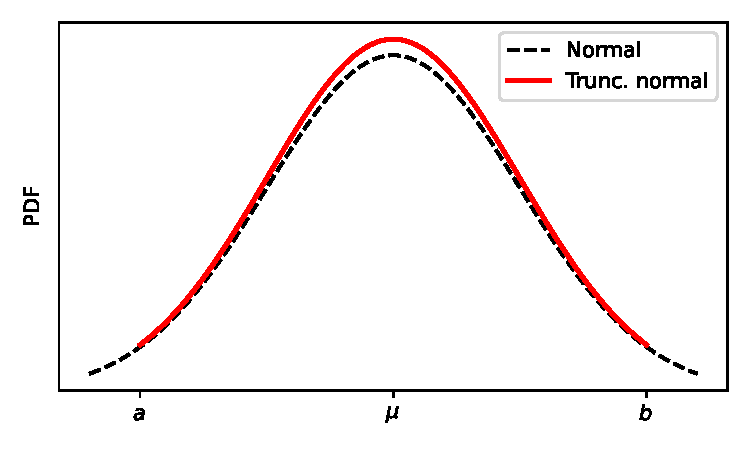
\includegraphics{solutions/unit06/unit06_ex2_PDF.pdf}
\caption{PDF of truncated normal}
\end{figure}

Compute the second non-central moment \(E[X^2]\) in four different ways:

\begin{enumerate}
\def\labelenumi{\arabic{enumi}.}
\item
  Use the fact that \(Var(X) = E[X^2] - E[X]^2\). Call the methods
  \texttt{mean()} and \texttt{var()} of the
  \href{https://docs.scipy.org/doc/scipy/reference/generated/scipy.stats.truncnorm.html}{truncated
  normal} implemented in SciPy to compute the (squared) mean and
  variance.

  \emph{Hint:} Import the truncated normal as follows:

\begin{verbatim}
from scipy.stats import truncnorm
\end{verbatim}
\item
  Use the \texttt{moment()} method of SciPy's truncated normal to
  directly compute the desired moment.
\item
  Use the \texttt{expect()} method of SciPy's truncated normal to
  compute the expectation \(E[X^2]\).
\item
  Use \href{https://en.wikipedia.org/wiki/Monte_Carlo_integration}{Monte
  Carlo integration} to compute the expectation \(E[X^2]\). There are
  numerous ways to do MC integration. In this exercise, we use a variant
  which draws random samples from a 2-dimensional uniform distribution
  to compute an area under the integrand:

  \begin{itemize}
  \tightlist
  \item
    To do this, define the integrand as
    \(x^2 \cdot f_t(x;a,b,\mu,\sigma)\) where \(f_t\) is the PDF of the
    truncated normal with parameters \(a\), \(b\), \(\mu\) and
    \(\sigma\).
  \item
    Draw random numbers in the rectangle which has length \(b-a\) and a
    height which is the maximum of the integrand on the integration
    interval \([a,b]\).
  \item
    Determine the fraction of sampled points that are below the
    integral, and use this to compute the area under the integrand.
  \end{itemize}

  The following figure illustrates this approach to integration. The
  blue dots are included in the integral whereas the red crosses are
  not:

  \begin{figure}
  \centering
  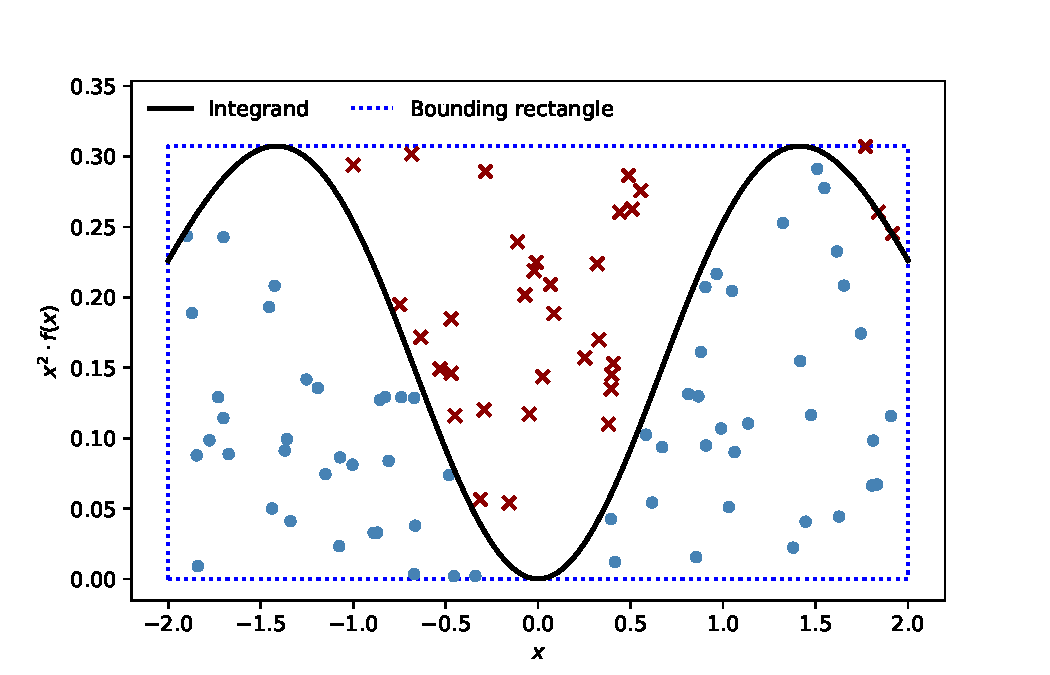
\includegraphics{solutions/unit06/unit06_ex2_MC.pdf}
  \caption{MC integration}
  \end{figure}

  This may not be the most practical way to do MC integration, and we
  will examine a more common approach in the next exercise.

  \emph{Note:} SciPy's truncated normal expects \emph{normalised}
  boundaries \(a\) and \(b\). Whenever the underlying distribution is
  \emph{not} standard normal, you have to pass \(z_a = (a-\mu)/\sigma\)
  and \(z_b = (b-\mu)/\sigma\) instead of \(a\) and \(b\) to all of
  \texttt{truncnorm}'s methods.
\end{enumerate}

    \hypertarget{exercise-3-multi-period-asset-returns}{%
\subsection{Exercise 3: Multi-period asset
returns}\label{exercise-3-multi-period-asset-returns}}

Consider an investor with initial assets \(a\) and a 2-period investment
horizon (we assume the investor does not change the asset position after
the first period).

Denote by \(R\) the total gross return over two periods, so that the
terminal wealth is given by \(W = a\cdot R\). The total gross return is
the product of the period-1 and period-2 gross returns,
\(R = R_1\cdot R_2\). We impose that per-period log returns
\(r_t = \log R_t\) are jointly normally distributed with mean
\(E[r_t] = \mu\), variance \(Var(r_t) = \sigma^2\) for \(t\in\{1,2\}\)
with a correlation coefficient \(Corr(r_1,r_2) = \rho\). Let \(a = 1\),
\(\mu = 0.04\), \(\sigma = 0.16\) and \(\rho = 0.5\).

\begin{enumerate}
\def\labelenumi{\arabic{enumi}.}
\item
  Derive the analytical expression for the expected total gross return
  after 2 periods.

  \emph{Hint:}

  \begin{itemize}
  \item
    Remember that since \((r_1,r_2)\) are jointly normally distributed,
    so is their sum, \(\log R = r_1 + r_2\).
  \item
    Moreover, if \(\log R\) is normally distributed with mean \(\mu_R\)
    and variance \(\sigma_R^2\), then \(R\) is
    \href{https://en.wikipedia.org/wiki/Log-normal_distribution}{log-normally}
    distributed and has the expected value

    \[E[R] = \exp\left(\mu_R + \frac{1}{2}\sigma_R^2 \right)\]
  \end{itemize}
\item
  Compute the expected terminal wealth after 2 periods using Monte Carlo
  simulation. To do this,

  \begin{enumerate}
  \def\labelenumii{\arabic{enumii}.}
  \item
    Draw \(N\) samples of multivariate normally distributed vectors
    \((r_{1i},r_{2i})\) using NumPy's
    \href{https://numpy.org/doc/stable/reference/random/generated/numpy.random.multivariate_normal.html}{multivariate\_normal()}.
  \item
    Compute the terminal wealth for each draw \(i\):
    \(W_i = a\exp(r_{1i})\exp(r_{2i})\).
  \item
    Compute the expected wealth as the sample average:

    \[E[W] \approx \overline{W} = \frac{1}{N}\sum_{i=1}^N W_i\]
  \end{enumerate}

  Make sure you get approximately the same result as in part 1 (you may
  need to increase the sample size if this is not the case).
\item
  Plot a histogram of the simulated total gross returns, and overlay it
  with the PDF of the log-normal distribution you derived in the first
  part.
\end{enumerate}

    \hypertarget{exercise-4-standard-error-and-increasing-sample-size}{%
\subsection{Exercise 4: Standard error and increasing sample
size}\label{exercise-4-standard-error-and-increasing-sample-size}}

Consider a setting in which we draw multiple samples indexed by \(k\)
such that these samples are increasing in the sample size \(N_k\), given
by \(N_k\) = 10, 50, 100, 500, 1000, 5000, 10000, 50000 and 100000.

The data for the \(k\)-th sample are \((x_{ik})_{i=1}^{N_k}\) where
\(i\) indexes some draw within the \(k\)-th sample. Assume that the data
are
\href{https://en.wikipedia.org/wiki/Log-normal_distribution}{log-normally}
distributed such that the underlying normal distribution has mean
\(\mu=0.5\) and variance \(\sigma^2 = 1.5^2\).

\begin{enumerate}
\def\labelenumi{\arabic{enumi}.}
\item
  For each sample size \(N_k\), use NumPy's
  \href{https://numpy.org/doc/stable/reference/random/generated/numpy.random.Generator.lognormal.html}{\texttt{lognormal()}}
  to draw a log-normally distributed sample.
\item
  For each sample, compute the sample mean and its standard error. As a
  reminder, the standard error of the \(k\)-th sample mean
  \(\overline{x}_k\) is defined as

  \[se(\overline{x}_k) = \sqrt{\frac{\widehat{\sigma}_{k}^2}{N_k}}\]

  where \(\widehat{\sigma}_{k}^2\) is the variance of residuals
  \(u_{ik} = x_{ik} - \overline{x}_k\) for each sample \(k\),

  \[\widehat{\sigma}_{k}^2 = \frac{1}{N_k-1}\sum_{i=1}^{N_k} u_{ik}^2\]
\item
  Plot the sample means for all samples, using the sample size on the
  \(x\)-axis and the estimated mean on the \(y\)-axis. Use the
  \(\log_{10}\) scale on the \(x\)-axis.

  \emph{Hint:} You can activate log scaling by calling
  \texttt{xscale(\textquotesingle{}log\textquotesingle{})}, or
  \texttt{set\_xscale(\textquotesingle{}log\textquotesingle{})} when
  using the object-oriented plotting interface.
\item
  Add a horizontal line showing the true mean (which is the same for all
  sample sizes).
\item
  Add confidence intervals (CI) for each sample size: use the interval
  \(\overline{x}_k \pm 2\times se(\overline{x}_k)\) to get a CI of
  approximately 95\%.
\end{enumerate}

    \hypertarget{exercise-5-the-jackknife}{%
\subsection{Exercise 5: The
jackknife}\label{exercise-5-the-jackknife}}

We continue with the setting from exercise 4, but instead of computing
the standard error as above, we now use a resampling technique known as
the \href{https://en.wikipedia.org/wiki/Jackknife_resampling}{jackknife}
to get the sample mean and its standard error.

\begin{enumerate}
\def\labelenumi{\arabic{enumi}.}
\tightlist
\item
  For each sample \(k\), compute \(N_k\) sample means
  \(\overline{x}_{-i,k}\) which are obtained by leaving out the \(i\)-th
  observation: \[
  \overline{x}_{-i,k} = \frac{1}{N_k-1}\sum_{j = 1, j \neq i}^{N_k} x_{jk} 
  \qquad i = 1,\dots,N_k
  \] where \(x_{jk}\) is the \(j\)-th draw in the \(k\)-th sample.
\item
  Compute the jackknife estimate of the sample mean as the average of
  these sub-sample means: \[
  \overline{x}_{k,jack} = \frac{1}{N_k}\sum_{i=1}^{N_k} \overline{x}_{-i,k}
  \] For the special case of a sample mean, it is straightforward to
  show that this is just the regular sample mean computed on the whole
  sample, \(\overline{x}_{k,jack} = \overline{x}_k\), where \[
  \overline{x}_k = \frac{1}{N_k}\sum_{i=1}^{N_k} x_{ik}
  \]
\item
  The jackknife estimate of the error variance for sample size \(N_k\)
  is then given by \[
  \begin{aligned}
  \widehat{var}(\overline{x}_k) 
      &= \frac{N_k - 1}{N_k} \sum_{i=1}^{N_k}\left(
              \overline{x}_{-i,k} - \overline{x}_{jack,k}\right)^2 \\
      &= \frac{1}{N_k(N_k-1)} \sum_{i=1}^{N_k}(x_{ik}-\overline{x}_k)^2
  \end{aligned}
  \] where the second line again follows as a special case if we are
  estimating the sample mean. The standard error of the sample mean is
  thus \[
  se(\overline{x}_k) = \sqrt{\widehat{var}(\overline{x}_k)}
  \]
\item
  Recreate the plot from exercise 4, but now use the jackknife estimate
  of the standard error instead.
\end{enumerate}

    \hypertarget{exercise-6-the-bootstrap}{%
\subsection{Exercise 6: The
bootstrap}\label{exercise-6-the-bootstrap}}

We continue with the setting from exercises 4 and 5, but now we use the
\href{https://en.wikipedia.org/wiki/Bootstrapping_(statistics)\#Case_resampling}{bootstrap}
to estimate the confidence intervals of the mean estimate.

\begin{enumerate}
\def\labelenumi{\arabic{enumi}.}
\tightlist
\item
  For each sample size \(N_k\) proceed as follows:

  \begin{enumerate}
  \def\labelenumii{\arabic{enumii}.}
  \tightlist
  \item
    Draw an initial sample of size \(N_k\) as before and compute the
    sample mean.
  \item
    Resample \(N_k\) observations by drawing from this initial sample
    \emph{with}\\
    \emph{replacement} using NumPy's
    \href{https://numpy.org/doc/stable/reference/random/generated/numpy.random.Generator.choice.html}{\texttt{choice()}}
    function.
  \item
    For each ``resample'', compute the sample mean. Say we have the
    \(j\)-th resample which consists of the draws
    \((x_{ik}^j)_{i=1}^{N_k}\), so we compute the \(j\)-th mean \[
    \overline{x}_{k}^j = \frac{1}{N_k} \sum_{i=1}^{N_k} x_{ik}^j
    \]
  \item
    Repeat steps 2 and 3 \(N_{bs} = 999\) times.
  \item
    Use these \(N_{bs}\) means to find the 2.5\% and 97.5\% percentiles
    of the mean estimate distribution, \(\overline{x}_k^{p2.5}\) and
    \(\overline{x}_k^{p97.5}\).
  \item
    The bootstrapped 95\% confidence interval is then given by
    \(\left[\overline{x}_k^{p2.5}, \overline{x}_k^{p97.5}\right]\).
  \end{enumerate}
\item
  Recreate the same plot as in exercises 4 and 5, but this time use the
  bootstrapped 95\% confidence interval you computed for each sample
  size.
\item
  For each sample size, store all bootstrapped means and use these to
  create a histogram of sample means. You will thus have to create 9
  histograms. Use vertical lines to indicate the 95\% confidence
  interval.
\end{enumerate}


\hypertarget{solutions}{%
\section{Solutions}\label{solutions}}

The solutions are also provided as Python scripts in the
\href{../lectures/solutions/unit06}{lectures/solutions/unit06/} folder.

    \hypertarget{solution-for-exercise-1}{%
\subsection{Solution for exercise 1}\label{solution-for-exercise-1}}

In the following solution, we create a figure with six panels (axes) and
iterate over these axes. In each iteration, we

\begin{enumerate}
\def\labelenumi{\arabic{enumi}.}
\tightlist
\item
  draw a random sample for the given (increasing) size;
\item
  plot the histogram using the current axes object; and
\item
  overlay the actual PDF.
\end{enumerate}

    \begin{tcolorbox}[breakable, size=fbox, boxrule=1pt, pad at break*=1mm,colback=cellbackground, colframe=cellborder]
\prompt{In}{incolor}{355}{\boxspacing}
\begin{Verbatim}[commandchars=\\\{\}]
\PY{k+kn}{import} \PY{n+nn}{matplotlib}\PY{n+nn}{.}\PY{n+nn}{pyplot} \PY{k}{as} \PY{n+nn}{plt}
\PY{k+kn}{import} \PY{n+nn}{numpy} \PY{k}{as} \PY{n+nn}{np}
\PY{k+kn}{from} \PY{n+nn}{numpy}\PY{n+nn}{.}\PY{n+nn}{random} \PY{k+kn}{import} \PY{n}{default\PYZus{}rng}
\PY{k+kn}{from} \PY{n+nn}{scipy}\PY{n+nn}{.}\PY{n+nn}{stats} \PY{k+kn}{import} \PY{n}{t} \PY{k}{as} \PY{n}{standard\PYZus{}t}

\PY{c+c1}{\PYZsh{} Sample sizes}
\PY{n}{Nobs} \PY{o}{=} \PY{n}{np}\PY{o}{.}\PY{n}{array}\PY{p}{(}\PY{p}{(}\PY{l+m+mi}{50}\PY{p}{,} \PY{l+m+mi}{100}\PY{p}{,} \PY{l+m+mi}{500}\PY{p}{,} \PY{l+m+mi}{1000}\PY{p}{,} \PY{l+m+mi}{5000}\PY{p}{,} \PY{l+m+mi}{10000}\PY{p}{)}\PY{p}{)}

\PY{c+c1}{\PYZsh{} degrees of freedom}
\PY{n}{df} \PY{o}{=} \PY{l+m+mi}{20}

\PY{c+c1}{\PYZsh{} Determine xlims such that we cover the (0.1, 99.9) percentiles}
\PY{c+c1}{\PYZsh{} of the distribution.}
\PY{n}{xmin}\PY{p}{,} \PY{n}{xmax} \PY{o}{=} \PY{n}{standard\PYZus{}t}\PY{o}{.}\PY{n}{ppf}\PY{p}{(}\PY{p}{(}\PY{l+m+mf}{0.001}\PY{p}{,} \PY{l+m+mf}{0.999}\PY{p}{)}\PY{p}{,} \PY{n}{df}\PY{o}{=}\PY{n}{df}\PY{p}{)}

\PY{n}{xvalues} \PY{o}{=} \PY{n}{np}\PY{o}{.}\PY{n}{linspace}\PY{p}{(}\PY{n}{xmin}\PY{p}{,} \PY{n}{xmax}\PY{p}{,} \PY{l+m+mi}{100}\PY{p}{)}
\PY{n}{pdf} \PY{o}{=} \PY{n}{standard\PYZus{}t}\PY{o}{.}\PY{n}{pdf}\PY{p}{(}\PY{n}{xvalues}\PY{p}{,} \PY{n}{df}\PY{o}{=}\PY{n}{df}\PY{p}{)}

\PY{n}{fig}\PY{p}{,} \PY{n}{ax} \PY{o}{=} \PY{n}{plt}\PY{o}{.}\PY{n}{subplots}\PY{p}{(}\PY{l+m+mi}{2}\PY{p}{,} \PY{l+m+mi}{3}\PY{p}{,} \PY{n}{sharex}\PY{o}{=}\PY{k+kc}{True}\PY{p}{,} \PY{n}{sharey}\PY{o}{=}\PY{k+kc}{True}\PY{p}{,} \PY{n}{figsize}\PY{o}{=}\PY{p}{(}\PY{l+m+mi}{10}\PY{p}{,} \PY{l+m+mi}{4}\PY{p}{)}\PY{p}{)}

\PY{c+c1}{\PYZsh{} initialize default RNG}
\PY{n}{rng} \PY{o}{=} \PY{n}{default\PYZus{}rng}\PY{p}{(}\PY{l+m+mi}{123}\PY{p}{)}

\PY{k}{for} \PY{n}{i}\PY{p}{,} \PY{n}{axes} \PY{o+ow}{in} \PY{n+nb}{enumerate}\PY{p}{(}\PY{n}{ax}\PY{o}{.}\PY{n}{flatten}\PY{p}{(}\PY{p}{)}\PY{p}{)}\PY{p}{:}
    \PY{c+c1}{\PYZsh{} Sample size to be plotted in current panel}
    \PY{n}{N} \PY{o}{=} \PY{n}{Nobs}\PY{p}{[}\PY{n}{i}\PY{p}{]}
    \PY{c+c1}{\PYZsh{} Draw sample of size N}
    \PY{n}{data} \PY{o}{=} \PY{n}{rng}\PY{o}{.}\PY{n}{standard\PYZus{}t}\PY{p}{(}\PY{n}{df}\PY{o}{=}\PY{n}{df}\PY{p}{,} \PY{n}{size}\PY{o}{=}\PY{n}{N}\PY{p}{)}

    \PY{c+c1}{\PYZsh{} plot histogram of given sample}
    \PY{n}{axes}\PY{o}{.}\PY{n}{hist}\PY{p}{(}\PY{n}{data}\PY{p}{,} \PY{n}{bins}\PY{o}{=}\PY{l+m+mi}{50}\PY{p}{,} \PY{n}{linewidth}\PY{o}{=}\PY{l+m+mf}{0.5}\PY{p}{,} \PY{n}{edgecolor}\PY{o}{=}\PY{l+s+s1}{\PYZsq{}}\PY{l+s+s1}{white}\PY{l+s+s1}{\PYZsq{}}\PY{p}{,} 
              \PY{n}{color}\PY{o}{=}\PY{l+s+s1}{\PYZsq{}}\PY{l+s+s1}{steelblue}\PY{l+s+s1}{\PYZsq{}}\PY{p}{,} \PY{n}{density}\PY{o}{=}\PY{k+kc}{True}\PY{p}{,} \PY{n}{label}\PY{o}{=}\PY{l+s+s1}{\PYZsq{}}\PY{l+s+s1}{Sample histogram}\PY{l+s+s1}{\PYZsq{}}\PY{p}{)}

    \PY{c+c1}{\PYZsh{} overlay actual PDF}
    \PY{n}{axes}\PY{o}{.}\PY{n}{plot}\PY{p}{(}\PY{n}{xvalues}\PY{p}{,} \PY{n}{pdf}\PY{p}{,} \PY{n}{color}\PY{o}{=}\PY{l+s+s1}{\PYZsq{}}\PY{l+s+s1}{red}\PY{l+s+s1}{\PYZsq{}}\PY{p}{,} \PY{n}{lw}\PY{o}{=}\PY{l+m+mf}{2.0}\PY{p}{,} \PY{n}{label}\PY{o}{=}\PY{l+s+s1}{\PYZsq{}}\PY{l+s+s1}{PDF}\PY{l+s+s1}{\PYZsq{}}\PY{p}{)}

    \PY{c+c1}{\PYZsh{} create text with current sample size}
    \PY{n}{axes}\PY{o}{.}\PY{n}{text}\PY{p}{(}\PY{l+m+mf}{0.05}\PY{p}{,} \PY{l+m+mf}{0.95}\PY{p}{,} \PY{l+s+sa}{f}\PY{l+s+s1}{\PYZsq{}}\PY{l+s+s1}{N=}\PY{l+s+si}{\PYZob{}}\PY{n}{N}\PY{l+s+si}{:}\PY{l+s+s1}{,d}\PY{l+s+si}{\PYZcb{}}\PY{l+s+s1}{\PYZsq{}}\PY{p}{,} \PY{n}{transform}\PY{o}{=}\PY{n}{axes}\PY{o}{.}\PY{n}{transAxes}\PY{p}{,} \PY{n}{va}\PY{o}{=}\PY{l+s+s1}{\PYZsq{}}\PY{l+s+s1}{top}\PY{l+s+s1}{\PYZsq{}}\PY{p}{)}

    \PY{n}{axes}\PY{o}{.}\PY{n}{set\PYZus{}xlim}\PY{p}{(}\PY{p}{(}\PY{n}{xmin}\PY{p}{,} \PY{n}{xmax}\PY{p}{)}\PY{p}{)}
    \PY{n}{axes}\PY{o}{.}\PY{n}{set\PYZus{}ylim}\PY{p}{(}\PY{p}{(}\PY{o}{\PYZhy{}}\PY{l+m+mf}{0.02}\PY{p}{,} \PY{l+m+mf}{1.3}\PY{p}{)}\PY{p}{)}

    \PY{c+c1}{\PYZsh{} plot legend only for the first panel}
    \PY{k}{if} \PY{n}{i} \PY{o}{==} \PY{l+m+mi}{0}\PY{p}{:}
        \PY{n}{axes}\PY{o}{.}\PY{n}{legend}\PY{p}{(}\PY{n}{loc}\PY{o}{=}\PY{l+s+s1}{\PYZsq{}}\PY{l+s+s1}{upper right}\PY{l+s+s1}{\PYZsq{}}\PY{p}{)}

\PY{c+c1}{\PYZsh{} compress space between individual panels}
\PY{n}{fig}\PY{o}{.}\PY{n}{tight\PYZus{}layout}\PY{p}{(}\PY{p}{)}
\PY{c+c1}{\PYZsh{} Add overall title}
\PY{n}{fig}\PY{o}{.}\PY{n}{suptitle}\PY{p}{(}\PY{l+s+s1}{\PYZsq{}}\PY{l+s+s1}{Draws from the standard\PYZhy{}t distribution}\PY{l+s+s1}{\PYZsq{}}\PY{p}{,} \PY{n}{fontsize}\PY{o}{=}\PY{l+m+mi}{16}\PY{p}{,} \PY{n}{y}\PY{o}{=}\PY{l+m+mf}{1.05}\PY{p}{)}
    
\end{Verbatim}
\end{tcolorbox}

            \begin{tcolorbox}[breakable, size=fbox, boxrule=.5pt, pad at break*=1mm, opacityfill=0]
\prompt{Out}{outcolor}{355}{\boxspacing}
\begin{Verbatim}[commandchars=\\\{\}]
Text(0.5, 1.05, 'Draws from the standard-t distribution')
\end{Verbatim}
\end{tcolorbox}
        
    \begin{center}
    \adjustimage{max size={0.9\linewidth}{0.9\paperheight}}{MLFP-part1_files/MLFP-part1_709_1.pdf}
    \end{center}
    
    A few comments on how we create the \(x\)-values and the plot range for
these graphs:

\begin{enumerate}
\def\labelenumi{\arabic{enumi}.}
\tightlist
\item
  In principle, we could draw arbitrarily large or small realised
  values, but we want to restrict the plot limits to a reasonable
  interval.
\item
  To find such an interval, we compute the percentiles corresponding to
  0.1\% and 99.9\%, which will cover almost any point we'd want to plot.
\item
  Moreover, we need to compute the \(x\)-values and evaluate the PDF at
  these points only once since these will remain unchanged for all
  sample sizes.
\end{enumerate}

Note also that the \texttt{subplots()} function returns a 2-dimensional
array (since we requested a \(2 \times 3\) layout). We iterate over the
\emph{flattened} array of axes objects instead of writing two nested
loops over rows and columns.

    \hypertarget{solution-for-exercise-2}{%
\subsection{Solution for exercise 2}\label{solution-for-exercise-2}}

Computing the second non-central moment using the first three methods is
straightforward. All you need to do is to make sure that you pass the
correct parameters to SciPy's \texttt{truncnorm} methods:

    \begin{tcolorbox}[breakable, size=fbox, boxrule=1pt, pad at break*=1mm,colback=cellbackground, colframe=cellborder]
\prompt{In}{incolor}{356}{\boxspacing}
\begin{Verbatim}[commandchars=\\\{\}]
\PY{k+kn}{import} \PY{n+nn}{numpy} \PY{k}{as} \PY{n+nn}{np}
\PY{k+kn}{from} \PY{n+nn}{scipy}\PY{n+nn}{.}\PY{n+nn}{stats} \PY{k+kn}{import} \PY{n}{truncnorm}

\PY{c+c1}{\PYZsh{} Parameters}
\PY{n}{mu} \PY{o}{=} \PY{l+m+mf}{0.0}
\PY{n}{sigma} \PY{o}{=} \PY{l+m+mf}{1.0}
\PY{n}{a} \PY{o}{=} \PY{n}{mu} \PY{o}{\PYZhy{}} \PY{l+m+mi}{2}\PY{o}{*}\PY{n}{sigma}
\PY{n}{b} \PY{o}{=} \PY{n}{mu} \PY{o}{+} \PY{l+m+mi}{2}\PY{o}{*}\PY{n}{sigma}

\PY{c+c1}{\PYZsh{} Standardised boundaries if underlying non\PYZhy{}truncated distr. is}
\PY{c+c1}{\PYZsh{} NOT standard normal}
\PY{n}{za} \PY{o}{=} \PY{p}{(}\PY{n}{a}\PY{o}{\PYZhy{}}\PY{n}{mu}\PY{p}{)}\PY{o}{/}\PY{n}{sigma}
\PY{n}{zb} \PY{o}{=} \PY{p}{(}\PY{n}{b}\PY{o}{\PYZhy{}}\PY{n}{mu}\PY{p}{)}\PY{o}{/}\PY{n}{sigma}

\PY{c+c1}{\PYZsh{} Method 1: Compute from E[X\PYZca{}2] = Var(X) + E[X]\PYZca{}2}
\PY{n}{var} \PY{o}{=} \PY{n}{truncnorm}\PY{o}{.}\PY{n}{var}\PY{p}{(}\PY{n}{za}\PY{p}{,} \PY{n}{zb}\PY{p}{,} \PY{n}{loc}\PY{o}{=}\PY{n}{mu}\PY{p}{,} \PY{n}{scale}\PY{o}{=}\PY{n}{sigma}\PY{p}{)}
\PY{n}{mean} \PY{o}{=} \PY{n}{truncnorm}\PY{o}{.}\PY{n}{mean}\PY{p}{(}\PY{n}{za}\PY{p}{,} \PY{n}{zb}\PY{p}{,} \PY{n}{loc}\PY{o}{=}\PY{n}{mu}\PY{p}{,} \PY{n}{scale}\PY{o}{=}\PY{n}{sigma}\PY{p}{)}
\PY{n}{m2\PYZus{}var\PYZus{}mean} \PY{o}{=} \PY{n}{var} \PY{o}{+} \PY{n}{mean} \PY{o}{*}\PY{o}{*} \PY{l+m+mf}{2.0}

\PY{c+c1}{\PYZsh{} Method 2: Compute using moment()}
\PY{n}{m2} \PY{o}{=} \PY{n}{truncnorm}\PY{o}{.}\PY{n}{moment}\PY{p}{(}\PY{l+m+mi}{2}\PY{p}{,} \PY{n}{za}\PY{p}{,} \PY{n}{zb}\PY{p}{,} \PY{n}{loc}\PY{o}{=}\PY{n}{mu}\PY{p}{,} \PY{n}{scale}\PY{o}{=}\PY{n}{sigma}\PY{p}{)}

\PY{c+c1}{\PYZsh{} Method 3: Compute moment using expect() function}
\PY{n}{m2\PYZus{}expect} \PY{o}{=} \PY{n}{truncnorm}\PY{o}{.}\PY{n}{expect}\PY{p}{(}\PY{k}{lambda} \PY{n}{x}\PY{p}{:} \PY{n}{x}\PY{o}{*}\PY{o}{*}\PY{l+m+mf}{2.0}\PY{p}{,} \PY{n}{args}\PY{o}{=}\PY{p}{(}\PY{n}{za}\PY{p}{,} \PY{n}{zb}\PY{p}{)}\PY{p}{,} 
                             \PY{n}{loc}\PY{o}{=}\PY{n}{mu}\PY{p}{,} \PY{n}{scale}\PY{o}{=}\PY{n}{sigma}\PY{p}{)}

\PY{n+nb}{print}\PY{p}{(}\PY{l+s+sa}{f}\PY{l+s+s1}{\PYZsq{}}\PY{l+s+s1}{Second non\PYZhy{}central moment, var + mean\PYZca{}2: }\PY{l+s+si}{\PYZob{}}\PY{n}{m2\PYZus{}var\PYZus{}mean}\PY{l+s+si}{:}\PY{l+s+s1}{.5e}\PY{l+s+si}{\PYZcb{}}\PY{l+s+s1}{\PYZsq{}}\PY{p}{)}
\PY{n+nb}{print}\PY{p}{(}\PY{l+s+sa}{f}\PY{l+s+s1}{\PYZsq{}}\PY{l+s+s1}{Second non\PYZhy{}central moment, moment(): }\PY{l+s+si}{\PYZob{}}\PY{n}{m2}\PY{l+s+si}{:}\PY{l+s+s1}{.5e}\PY{l+s+si}{\PYZcb{}}\PY{l+s+s1}{\PYZsq{}}\PY{p}{)}
\PY{n+nb}{print}\PY{p}{(}\PY{l+s+sa}{f}\PY{l+s+s1}{\PYZsq{}}\PY{l+s+s1}{Second non\PYZhy{}central moment, expect(): }\PY{l+s+si}{\PYZob{}}\PY{n}{m2\PYZus{}expect}\PY{l+s+si}{:}\PY{l+s+s1}{.5e}\PY{l+s+si}{\PYZcb{}}\PY{l+s+s1}{\PYZsq{}}\PY{p}{)}
\end{Verbatim}
\end{tcolorbox}

    \begin{Verbatim}[commandchars=\\\{\}]
Second non-central moment, var + mean\^{}2: 7.73741e-01
Second non-central moment, moment(): 7.73741e-01
Second non-central moment, expect(): 7.73741e-01
    \end{Verbatim}

    The fourth method is more involved. We first define the integrand as
follows:

    \begin{tcolorbox}[breakable, size=fbox, boxrule=1pt, pad at break*=1mm,colback=cellbackground, colframe=cellborder]
\prompt{In}{incolor}{357}{\boxspacing}
\begin{Verbatim}[commandchars=\\\{\}]
\PY{c+c1}{\PYZsh{} Function to compute integrand}
\PY{k}{def} \PY{n+nf}{f\PYZus{}integrand}\PY{p}{(}\PY{n}{x}\PY{p}{,} \PY{n}{a}\PY{p}{,} \PY{n}{b}\PY{p}{,} \PY{n}{mu}\PY{p}{,} \PY{n}{sigma}\PY{p}{)}\PY{p}{:}
    \PY{c+c1}{\PYZsh{} Transform to boundaries required by SciPy\PYZsq{}s truncnorm}
    \PY{n}{za} \PY{o}{=} \PY{p}{(}\PY{n}{a} \PY{o}{\PYZhy{}} \PY{n}{mu}\PY{p}{)} \PY{o}{/} \PY{n}{sigma}
    \PY{n}{zb} \PY{o}{=} \PY{p}{(}\PY{n}{b} \PY{o}{\PYZhy{}} \PY{n}{mu}\PY{p}{)} \PY{o}{/} \PY{n}{sigma}
    \PY{c+c1}{\PYZsh{} Evaluate truncated normal PDF}
    \PY{n}{pdf} \PY{o}{=} \PY{n}{truncnorm}\PY{o}{.}\PY{n}{pdf}\PY{p}{(}\PY{n}{x}\PY{p}{,} \PY{n}{za}\PY{p}{,} \PY{n}{zb}\PY{p}{,} \PY{n}{loc}\PY{o}{=}\PY{n}{mu}\PY{p}{,} \PY{n}{scale}\PY{o}{=}\PY{n}{sigma}\PY{p}{)}
    \PY{c+c1}{\PYZsh{} Compute integrand x\PYZca{}2 * f(x)}
    \PY{n}{result} \PY{o}{=} \PY{n}{x} \PY{o}{*}\PY{o}{*} \PY{l+m+mf}{2.0} \PY{o}{*} \PY{n}{pdf}
    \PY{k}{return} \PY{n}{result}
\end{Verbatim}
\end{tcolorbox}

    The remainder of the Monte Carlo code look as follows:

    \begin{tcolorbox}[breakable, size=fbox, boxrule=1pt, pad at break*=1mm,colback=cellbackground, colframe=cellborder]
\prompt{In}{incolor}{358}{\boxspacing}
\begin{Verbatim}[commandchars=\\\{\}]
\PY{k+kn}{from} \PY{n+nn}{numpy}\PY{n+nn}{.}\PY{n+nn}{random} \PY{k+kn}{import} \PY{n}{default\PYZus{}rng}

\PY{c+c1}{\PYZsh{} Initialise RNG}
\PY{n}{rng} \PY{o}{=} \PY{n}{default\PYZus{}rng}\PY{p}{(}\PY{l+m+mi}{123}\PY{p}{)}
\PY{c+c1}{\PYZsh{} Sample size for Monte Carlo integration}
\PY{n}{Nsample} \PY{o}{=} \PY{l+m+mi}{50000}

\PY{c+c1}{\PYZsh{} x\PYZhy{}values should be uniformly distributed on [a, b]}
\PY{n}{xsample} \PY{o}{=} \PY{n}{rng}\PY{o}{.}\PY{n}{uniform}\PY{p}{(}\PY{n}{a}\PY{p}{,} \PY{n}{b}\PY{p}{,} \PY{n}{size}\PY{o}{=}\PY{n}{Nsample}\PY{p}{)}
\PY{c+c1}{\PYZsh{} Alternatively we can also just use equidistant x\PYZhy{}values, in}
\PY{c+c1}{\PYZsh{} low\PYZhy{}dimensional problems it makes no difference.}
\PY{c+c1}{\PYZsh{} xsample = np.linspace(a, b, Nsamples)}

\PY{c+c1}{\PYZsh{} Evaluate integrand at sampled x\PYZhy{}values}
\PY{n}{integrand} \PY{o}{=} \PY{n}{f\PYZus{}integrand}\PY{p}{(}\PY{n}{xsample}\PY{p}{,} \PY{n}{a}\PY{p}{,} \PY{n}{b}\PY{p}{,} \PY{n}{mu}\PY{p}{,} \PY{n}{sigma}\PY{p}{)}

\PY{c+c1}{\PYZsh{} Compute size of bounding rectangle:}
\PY{c+c1}{\PYZsh{} the height is taken as the largest realisation of the integrand.}
\PY{n}{length} \PY{o}{=} \PY{n}{b} \PY{o}{\PYZhy{}} \PY{n}{a}
\PY{n}{height} \PY{o}{=} \PY{n}{np}\PY{o}{.}\PY{n}{amax}\PY{p}{(}\PY{n}{integrand}\PY{p}{)}
\PY{n}{area} \PY{o}{=} \PY{n}{height} \PY{o}{*} \PY{n}{length}
\PY{c+c1}{\PYZsh{} draw y\PYZhy{}values from uniform distribution on [0, height]}
\PY{n}{ysample} \PY{o}{=} \PY{n}{rng}\PY{o}{.}\PY{n}{uniform}\PY{p}{(}\PY{l+m+mi}{0}\PY{p}{,} \PY{n}{height}\PY{p}{,} \PY{n}{size}\PY{o}{=}\PY{n}{Nsample}\PY{p}{)}
\PY{c+c1}{\PYZsh{} Compute fraction of points that are underneath the PDF}
\PY{n}{frac} \PY{o}{=} \PY{n}{np}\PY{o}{.}\PY{n}{mean}\PY{p}{(}\PY{n}{ysample} \PY{o}{\PYZlt{}}\PY{o}{=} \PY{n}{integrand}\PY{p}{)}
\PY{n}{integral\PYZus{}MC} \PY{o}{=} \PY{n}{frac} \PY{o}{*} \PY{n}{area}

\PY{n+nb}{print}\PY{p}{(}\PY{l+s+sa}{f}\PY{l+s+s1}{\PYZsq{}}\PY{l+s+s1}{Second non\PYZhy{}central moment, MC integration: }\PY{l+s+si}{\PYZob{}}\PY{n}{integral\PYZus{}MC}\PY{l+s+si}{:}\PY{l+s+s1}{.5e}\PY{l+s+si}{\PYZcb{}}\PY{l+s+s1}{\PYZsq{}}\PY{p}{)}
\end{Verbatim}
\end{tcolorbox}

    \begin{Verbatim}[commandchars=\\\{\}]
Second non-central moment, MC integration: 7.72828e-01
    \end{Verbatim}

    You might have noticed that MC integration is not the fastest to
converge, but using 50000 draws is sufficient to get somewhat close to
the other three methods.

In this case we do not actually need Monte Carlo methods, because the
dimensionality of the problem is so low. We could just as well have used
a dense deterministic rectangular grid instead of randomly-drawn points.

The entire Python script which also generates the graphs displayed in
the exercise can be found in the
\href{../lectures/solutions/unit7}{solutions} folder

    \hypertarget{solution-for-exercise-3}{%
\subsection{Solution for exercise 3}\label{solution-for-exercise-3}}

\textbf{Part 1}

The first part is purely analytical. We use it to verify that the code
in part 2 yields the correct result.

Since \((r_1, r_2)\) are jointly normal, a standard result is that their
sum \(r_1 + r_2\) is normally distributed with mean and variance given
by

\[\mu_{rr} = E[r_1 + r_2] = 2\mu \]

\[
\sigma^2_{rr} = Var(r_1+r_2) = Var(r_1) + Var(r_2) + 2\cdot Cov(r_1,r_2) = 2\sigma^2 + 2\rho\sigma^2 
\]

This is even simpler than the usual formulas since both per-period log
returns have the same mean and variance.

Moreover, since \(\log R = r_1 + r_2\) is normally distributed, \(R\) is
log-normally distributed and has the expected value \[
E[R] = \exp\left(\mu_{rr} + \frac{1}{2}\sigma_{rr}^2 \right)
    = \exp\left(2\mu + (1+\rho) \sigma^2 \right)
\] Since \(a = 1\), this is also the expected value of terminal wealth
\(W\).

We can plug in the parameter values to compute the numerical value:

    \begin{tcolorbox}[breakable, size=fbox, boxrule=1pt, pad at break*=1mm,colback=cellbackground, colframe=cellborder]
\prompt{In}{incolor}{359}{\boxspacing}
\begin{Verbatim}[commandchars=\\\{\}]
\PY{k+kn}{import} \PY{n+nn}{numpy} \PY{k}{as} \PY{n+nn}{np}

\PY{c+c1}{\PYZsh{} Parameters}
\PY{n}{a} \PY{o}{=} \PY{l+m+mf}{1.0}                         \PY{c+c1}{\PYZsh{} Initial assets}
\PY{n}{mu} \PY{o}{=} \PY{n}{np}\PY{o}{.}\PY{n}{array}\PY{p}{(}\PY{p}{(}\PY{l+m+mf}{0.04}\PY{p}{,} \PY{l+m+mf}{0.04}\PY{p}{)}\PY{p}{)}     \PY{c+c1}{\PYZsh{} average log returns}
\PY{n}{sigma} \PY{o}{=} \PY{l+m+mf}{0.16}                    \PY{c+c1}{\PYZsh{} std. dev. of log returns}
\PY{n}{rho} \PY{o}{=} \PY{l+m+mf}{0.5}                       \PY{c+c1}{\PYZsh{} serial correlation}

\PY{c+c1}{\PYZsh{} Exact expectation}
\PY{n}{var\PYZus{}rr} \PY{o}{=} \PY{l+m+mf}{2.0} \PY{o}{*} \PY{n}{sigma} \PY{o}{*}\PY{o}{*} \PY{l+m+mf}{2.0} \PY{o}{+} \PY{l+m+mf}{2.0} \PY{o}{*} \PY{n}{rho} \PY{o}{*} \PY{n}{sigma} \PY{o}{*}\PY{o}{*} \PY{l+m+mf}{2.0}
\PY{n}{sigma\PYZus{}rr} \PY{o}{=} \PY{n}{np}\PY{o}{.}\PY{n}{sqrt}\PY{p}{(}\PY{n}{var\PYZus{}rr}\PY{p}{)}
\PY{n}{mu\PYZus{}rr} \PY{o}{=} \PY{n}{np}\PY{o}{.}\PY{n}{sum}\PY{p}{(}\PY{n}{mu}\PY{p}{)}

\PY{n}{exp\PYZus{}exact} \PY{o}{=} \PY{n}{a} \PY{o}{*} \PY{n}{np}\PY{o}{.}\PY{n}{exp}\PY{p}{(}\PY{n}{mu\PYZus{}rr} \PY{o}{+} \PY{n}{sigma\PYZus{}rr} \PY{o}{*}\PY{o}{*} \PY{l+m+mf}{2.0} \PY{o}{/} \PY{l+m+mf}{2.0}\PY{p}{)}

\PY{n+nb}{print}\PY{p}{(}\PY{l+s+sa}{f}\PY{l+s+s1}{\PYZsq{}}\PY{l+s+s1}{Expected portfolio value (exact): }\PY{l+s+si}{\PYZob{}}\PY{n}{exp\PYZus{}exact}\PY{l+s+si}{:}\PY{l+s+s1}{.4f}\PY{l+s+si}{\PYZcb{}}\PY{l+s+s1}{\PYZsq{}}\PY{p}{)}
\end{Verbatim}
\end{tcolorbox}

    \begin{Verbatim}[commandchars=\\\{\}]
Expected portfolio value (exact): 1.1257
    \end{Verbatim}

    \textbf{Parts 2 and 3}

To perform the Monte Carlo simulation, we need to define the vector of
means and the variance-covariance matrix which we can pass to NumPy's
\texttt{multivariate\_normal()} to sample returns \((r_1, r_2)\):

    \begin{tcolorbox}[breakable, size=fbox, boxrule=1pt, pad at break*=1mm,colback=cellbackground, colframe=cellborder]
\prompt{In}{incolor}{360}{\boxspacing}
\begin{Verbatim}[commandchars=\\\{\}]
\PY{k+kn}{import} \PY{n+nn}{numpy} \PY{k}{as} \PY{n+nn}{np}
\PY{k+kn}{from} \PY{n+nn}{numpy}\PY{n+nn}{.}\PY{n+nn}{random} \PY{k+kn}{import} \PY{n}{default\PYZus{}rng}
\PY{k+kn}{from} \PY{n+nn}{scipy}\PY{n+nn}{.}\PY{n+nn}{stats} \PY{k+kn}{import} \PY{n}{lognorm}

\PY{c+c1}{\PYZsh{} Parameters}
\PY{n}{a} \PY{o}{=} \PY{l+m+mf}{1.0}                         \PY{c+c1}{\PYZsh{} Initial assets}
\PY{n}{mu} \PY{o}{=} \PY{n}{np}\PY{o}{.}\PY{n}{array}\PY{p}{(}\PY{p}{(}\PY{l+m+mf}{0.04}\PY{p}{,} \PY{l+m+mf}{0.04}\PY{p}{)}\PY{p}{)}     \PY{c+c1}{\PYZsh{} average log returns}
\PY{n}{sigma} \PY{o}{=} \PY{l+m+mf}{0.16}                    \PY{c+c1}{\PYZsh{} std. dev. of log returns}
\PY{n}{rho} \PY{o}{=} \PY{l+m+mf}{0.5}                       \PY{c+c1}{\PYZsh{} serial correlation}

\PY{c+c1}{\PYZsh{} Covariance}
\PY{n}{cov} \PY{o}{=} \PY{n}{rho}\PY{o}{*}\PY{n}{sigma}\PY{o}{*}\PY{o}{*}\PY{l+m+mf}{2.0}
\PY{c+c1}{\PYZsh{} variance\PYZhy{}covariance matrix}
\PY{n}{vcv} \PY{o}{=} \PY{n}{np}\PY{o}{.}\PY{n}{array}\PY{p}{(}\PY{p}{[}\PY{p}{[}\PY{n}{sigma}\PY{o}{*}\PY{o}{*}\PY{l+m+mf}{2.0}\PY{p}{,} \PY{n}{cov}\PY{p}{]}\PY{p}{,}
                \PY{p}{[}\PY{n}{cov}\PY{p}{,} \PY{n}{sigma}\PY{o}{*}\PY{o}{*}\PY{l+m+mf}{2.0}\PY{p}{]}\PY{p}{]}\PY{p}{)}

\PY{n}{Nsample} \PY{o}{=} \PY{l+m+mi}{5000000}
\PY{n}{rng} \PY{o}{=} \PY{n}{default\PYZus{}rng}\PY{p}{(}\PY{l+m+mi}{123}\PY{p}{)}
\PY{c+c1}{\PYZsh{} Draw MV normal samples: each row corresponds to one draw}
\PY{n}{samples} \PY{o}{=} \PY{n}{rng}\PY{o}{.}\PY{n}{multivariate\PYZus{}normal}\PY{p}{(}\PY{n}{mean}\PY{o}{=}\PY{n}{mu}\PY{p}{,} \PY{n}{cov}\PY{o}{=}\PY{n}{vcv}\PY{p}{,} \PY{n}{size}\PY{o}{=}\PY{n}{Nsample}\PY{p}{)}

\PY{c+c1}{\PYZsh{} Evaluate total gross return at sampled points:}
\PY{c+c1}{\PYZsh{}   R = exp(r\PYZus{}1) * exp(r\PYZus{}2)}
\PY{n}{returns} \PY{o}{=} \PY{n}{np}\PY{o}{.}\PY{n}{prod}\PY{p}{(}\PY{n}{np}\PY{o}{.}\PY{n}{exp}\PY{p}{(}\PY{n}{samples}\PY{p}{)}\PY{p}{,} \PY{n}{axis}\PY{o}{=}\PY{l+m+mi}{1}\PY{p}{)}
\PY{c+c1}{\PYZsh{} Sampled terminal wealth after 2 periods}
\PY{n}{wealth} \PY{o}{=} \PY{n}{a} \PY{o}{*} \PY{n}{returns}
\PY{c+c1}{\PYZsh{} Expected terminal wealth}
\PY{n}{exp\PYZus{}MC} \PY{o}{=} \PY{n}{np}\PY{o}{.}\PY{n}{mean}\PY{p}{(}\PY{n}{wealth}\PY{p}{)}

\PY{n+nb}{print}\PY{p}{(}\PY{l+s+sa}{f}\PY{l+s+s1}{\PYZsq{}}\PY{l+s+s1}{Expected portfolio value (MC): }\PY{l+s+si}{\PYZob{}}\PY{n}{exp\PYZus{}MC}\PY{l+s+si}{:}\PY{l+s+s1}{.4f}\PY{l+s+si}{\PYZcb{}}\PY{l+s+s1}{\PYZsq{}}\PY{p}{)}
\end{Verbatim}
\end{tcolorbox}

    \begin{Verbatim}[commandchars=\\\{\}]
Expected portfolio value (MC): 1.1256
    \end{Verbatim}

    Finally, we use the sampled points and the \texttt{pdf()} method of
SciPy's
\href{https://docs.scipy.org/doc/scipy/reference/generated/scipy.stats.lognorm.html}{lognorm}
to plot the histogram and the true PDF.

    \begin{tcolorbox}[breakable, size=fbox, boxrule=1pt, pad at break*=1mm,colback=cellbackground, colframe=cellborder]
\prompt{In}{incolor}{361}{\boxspacing}
\begin{Verbatim}[commandchars=\\\{\}]
\PY{k+kn}{import} \PY{n+nn}{matplotlib}\PY{n+nn}{.}\PY{n+nn}{pyplot} \PY{k}{as} \PY{n+nn}{plt}

\PY{n}{fig}\PY{p}{,} \PY{n}{ax} \PY{o}{=} \PY{n}{plt}\PY{o}{.}\PY{n}{subplots}\PY{p}{(}\PY{l+m+mi}{1}\PY{p}{,} \PY{l+m+mi}{1}\PY{p}{)}

\PY{n}{ax}\PY{o}{.}\PY{n}{hist}\PY{p}{(}\PY{n}{returns}\PY{p}{,} \PY{n}{bins}\PY{o}{=}\PY{l+m+mi}{75}\PY{p}{,} \PY{n}{density}\PY{o}{=}\PY{k+kc}{True}\PY{p}{,} \PY{n}{color}\PY{o}{=}\PY{l+s+s1}{\PYZsq{}}\PY{l+s+s1}{steelblue}\PY{l+s+s1}{\PYZsq{}}\PY{p}{,} \PY{n}{lw}\PY{o}{=}\PY{l+m+mf}{0.5}\PY{p}{,}
        \PY{n}{edgecolor}\PY{o}{=}\PY{l+s+s1}{\PYZsq{}}\PY{l+s+s1}{white}\PY{l+s+s1}{\PYZsq{}}\PY{p}{,} \PY{n}{alpha}\PY{o}{=}\PY{l+m+mf}{.8}\PY{p}{,} \PY{n}{label}\PY{o}{=}\PY{l+s+s1}{\PYZsq{}}\PY{l+s+s1}{Sample}\PY{l+s+s1}{\PYZsq{}}\PY{p}{)}

\PY{c+c1}{\PYZsh{} Plot log\PYZhy{}normal PDF of total gross return}
\PY{n}{xmin}\PY{p}{,} \PY{n}{xmax} \PY{o}{=} \PY{n}{np}\PY{o}{.}\PY{n}{amin}\PY{p}{(}\PY{n}{returns}\PY{p}{)}\PY{p}{,} \PY{n}{np}\PY{o}{.}\PY{n}{amax}\PY{p}{(}\PY{n}{returns}\PY{p}{)}
\PY{n}{xvalues} \PY{o}{=} \PY{n}{np}\PY{o}{.}\PY{n}{linspace}\PY{p}{(}\PY{n}{xmin}\PY{p}{,} \PY{n}{xmax}\PY{p}{,} \PY{l+m+mi}{200}\PY{p}{)}
\PY{n}{pdf} \PY{o}{=} \PY{n}{lognorm}\PY{o}{.}\PY{n}{pdf}\PY{p}{(}\PY{n}{xvalues}\PY{p}{,} \PY{n}{s}\PY{o}{=}\PY{n}{sigma\PYZus{}rr}\PY{p}{,} \PY{n}{loc}\PY{o}{=}\PY{n}{mu\PYZus{}rr}\PY{p}{)}
\PY{n}{ax}\PY{o}{.}\PY{n}{plot}\PY{p}{(}\PY{n}{xvalues}\PY{p}{,} \PY{n}{pdf}\PY{p}{,} \PY{n}{c}\PY{o}{=}\PY{l+s+s1}{\PYZsq{}}\PY{l+s+s1}{red}\PY{l+s+s1}{\PYZsq{}}\PY{p}{,} \PY{n}{lw}\PY{o}{=}\PY{l+m+mf}{1.5}\PY{p}{,} \PY{n}{label}\PY{o}{=}\PY{l+s+s1}{\PYZsq{}}\PY{l+s+s1}{PDF}\PY{l+s+s1}{\PYZsq{}}\PY{p}{)}

\PY{c+c1}{\PYZsh{} Add line with true expected value}
\PY{n}{ax}\PY{o}{.}\PY{n}{axvline}\PY{p}{(}\PY{n}{exp\PYZus{}exact}\PY{p}{,} \PY{n}{lw}\PY{o}{=}\PY{l+m+mf}{1.0}\PY{p}{,} \PY{n}{color}\PY{o}{=}\PY{l+s+s1}{\PYZsq{}}\PY{l+s+s1}{black}\PY{l+s+s1}{\PYZsq{}}\PY{p}{,} \PY{n}{ls}\PY{o}{=}\PY{l+s+s1}{\PYZsq{}}\PY{l+s+s1}{\PYZhy{}\PYZhy{}}\PY{l+s+s1}{\PYZsq{}}\PY{p}{,} \PY{n}{label}\PY{o}{=}\PY{l+s+s1}{\PYZsq{}}\PY{l+s+s1}{Mean}\PY{l+s+s1}{\PYZsq{}}\PY{p}{)}

\PY{n}{ax}\PY{o}{.}\PY{n}{set\PYZus{}xlabel}\PY{p}{(}\PY{l+s+s1}{\PYZsq{}}\PY{l+s+s1}{Total gross return \PYZdl{}R\PYZdl{}}\PY{l+s+s1}{\PYZsq{}}\PY{p}{)}
\PY{n}{ax}\PY{o}{.}\PY{n}{set\PYZus{}ylabel}\PY{p}{(}\PY{l+s+s1}{\PYZsq{}}\PY{l+s+s1}{Density}\PY{l+s+s1}{\PYZsq{}}\PY{p}{)}
\PY{n}{ax}\PY{o}{.}\PY{n}{legend}\PY{p}{(}\PY{n}{loc}\PY{o}{=}\PY{l+s+s1}{\PYZsq{}}\PY{l+s+s1}{upper right}\PY{l+s+s1}{\PYZsq{}}\PY{p}{,} \PY{n}{frameon}\PY{o}{=}\PY{k+kc}{False}\PY{p}{)}
\end{Verbatim}
\end{tcolorbox}

            \begin{tcolorbox}[breakable, size=fbox, boxrule=.5pt, pad at break*=1mm, opacityfill=0]
\prompt{Out}{outcolor}{361}{\boxspacing}
\begin{Verbatim}[commandchars=\\\{\}]
<matplotlib.legend.Legend at 0x7fd02c92d5d0>
\end{Verbatim}
\end{tcolorbox}
        
    \begin{center}
    \adjustimage{max size={0.9\linewidth}{0.9\paperheight}}{MLFP-part1_files/MLFP-part1_723_1.pdf}
    \end{center}
    
    The dashed black line shows the analytically derived expected total
gross return.

    \hypertarget{solution-for-exercise-4}{%
\subsection{Solution for exercise 4}\label{solution-for-exercise-4}}

We solve the exercise by iterating over all sample sizes, drawing a new
log-normal sample and computing the sample mean and standard error.
These are stored in the arrays \texttt{mean\_hat} and \texttt{std\_err},
which we then use the generate the plot.

    \begin{tcolorbox}[breakable, size=fbox, boxrule=1pt, pad at break*=1mm,colback=cellbackground, colframe=cellborder]
\prompt{In}{incolor}{362}{\boxspacing}
\begin{Verbatim}[commandchars=\\\{\}]
\PY{k+kn}{import} \PY{n+nn}{numpy} \PY{k}{as} \PY{n+nn}{np}
\PY{k+kn}{from} \PY{n+nn}{numpy}\PY{n+nn}{.}\PY{n+nn}{random} \PY{k+kn}{import} \PY{n}{default\PYZus{}rng}
\PY{k+kn}{import} \PY{n+nn}{matplotlib}\PY{n+nn}{.}\PY{n+nn}{pyplot} \PY{k}{as} \PY{n+nn}{plt}

\PY{n}{sample\PYZus{}sizes} \PY{o}{=} \PY{n}{np}\PY{o}{.}\PY{n}{array}\PY{p}{(}\PY{p}{[}\PY{l+m+mi}{10}\PY{p}{,} \PY{l+m+mi}{50}\PY{p}{,} \PY{l+m+mi}{100}\PY{p}{,} \PY{l+m+mi}{500}\PY{p}{,} \PY{l+m+mi}{1000}\PY{p}{,} \PY{l+m+mi}{5000}\PY{p}{,} \PY{l+m+mi}{10000}\PY{p}{,} \PY{l+m+mi}{50000}\PY{p}{,} \PY{l+m+mi}{100000}\PY{p}{]}\PY{p}{)}
\PY{c+c1}{\PYZsh{} initialize default RNG}
\PY{n}{rng} \PY{o}{=} \PY{n}{default\PYZus{}rng}\PY{p}{(}\PY{l+m+mi}{123}\PY{p}{)}

\PY{c+c1}{\PYZsh{} Parameters of underlying normal distribution}
\PY{n}{mu} \PY{o}{=} \PY{l+m+mf}{0.5}
\PY{n}{sigma} \PY{o}{=} \PY{l+m+mf}{1.5}

\PY{c+c1}{\PYZsh{} Array to store estimated mean for each sample size}
\PY{n}{mean\PYZus{}hat} \PY{o}{=} \PY{n}{np}\PY{o}{.}\PY{n}{zeros}\PY{p}{(}\PY{n+nb}{len}\PY{p}{(}\PY{n}{sample\PYZus{}sizes}\PY{p}{)}\PY{p}{)}
\PY{c+c1}{\PYZsh{} Array to store std. error for each sample size}
\PY{n}{std\PYZus{}err} \PY{o}{=} \PY{n}{np}\PY{o}{.}\PY{n}{zeros\PYZus{}like}\PY{p}{(}\PY{n}{mean\PYZus{}hat}\PY{p}{)}

\PY{k}{for} \PY{n}{k}\PY{p}{,} \PY{n}{N} \PY{o+ow}{in} \PY{n+nb}{enumerate}\PY{p}{(}\PY{n}{sample\PYZus{}sizes}\PY{p}{)}\PY{p}{:}
    \PY{n}{data} \PY{o}{=} \PY{n}{rng}\PY{o}{.}\PY{n}{lognormal}\PY{p}{(}\PY{n}{mean}\PY{o}{=}\PY{n}{mu}\PY{p}{,} \PY{n}{sigma}\PY{o}{=}\PY{n}{sigma}\PY{p}{,} \PY{n}{size}\PY{o}{=}\PY{n}{N}\PY{p}{)}
    \PY{c+c1}{\PYZsh{} sample mean}
    \PY{n}{x\PYZus{}k} \PY{o}{=} \PY{n}{np}\PY{o}{.}\PY{n}{mean}\PY{p}{(}\PY{n}{data}\PY{p}{)}
    \PY{c+c1}{\PYZsh{} residuals around mean}
    \PY{n}{resid} \PY{o}{=} \PY{n}{data} \PY{o}{\PYZhy{}} \PY{n}{x\PYZus{}k}
    \PY{c+c1}{\PYZsh{} Residual variance}
    \PY{n}{var\PYZus{}resid} \PY{o}{=} \PY{n}{np}\PY{o}{.}\PY{n}{sum}\PY{p}{(}\PY{n}{resid}\PY{o}{*}\PY{o}{*}\PY{l+m+mf}{2.0}\PY{p}{)} \PY{o}{/} \PY{p}{(}\PY{n}{N}\PY{o}{\PYZhy{}}\PY{l+m+mi}{1}\PY{p}{)}
    \PY{c+c1}{\PYZsh{} std. error of mean estimate}
    \PY{n}{se\PYZus{}k} \PY{o}{=} \PY{n}{np}\PY{o}{.}\PY{n}{sqrt}\PY{p}{(}\PY{n}{var\PYZus{}resid} \PY{o}{/} \PY{n}{N}\PY{p}{)}

    \PY{c+c1}{\PYZsh{} store sample estimates in array}
    \PY{n}{mean\PYZus{}hat}\PY{p}{[}\PY{n}{k}\PY{p}{]} \PY{o}{=} \PY{n}{x\PYZus{}k}
    \PY{n}{std\PYZus{}err}\PY{p}{[}\PY{n}{k}\PY{p}{]} \PY{o}{=} \PY{n}{se\PYZus{}k}

\PY{c+c1}{\PYZsh{} Plot results}
\PY{n}{plt}\PY{o}{.}\PY{n}{plot}\PY{p}{(}\PY{n}{sample\PYZus{}sizes}\PY{p}{,} \PY{n}{mean\PYZus{}hat}\PY{p}{,} \PY{n}{lw}\PY{o}{=}\PY{l+m+mf}{2.0}\PY{p}{,} \PY{n}{label}\PY{o}{=}\PY{l+s+s1}{\PYZsq{}}\PY{l+s+s1}{Estim. mean}\PY{l+s+s1}{\PYZsq{}}\PY{p}{)}

\PY{c+c1}{\PYZsh{} Add line indicating true mean of log\PYZhy{}normal}
\PY{n}{mean} \PY{o}{=} \PY{n}{np}\PY{o}{.}\PY{n}{exp}\PY{p}{(}\PY{n}{mu} \PY{o}{+} \PY{n}{sigma}\PY{o}{*}\PY{o}{*}\PY{l+m+mf}{2.0} \PY{o}{/} \PY{l+m+mf}{2.0}\PY{p}{)}
\PY{n}{plt}\PY{o}{.}\PY{n}{axhline}\PY{p}{(}\PY{n}{mean}\PY{p}{,} \PY{n}{lw}\PY{o}{=}\PY{l+m+mf}{1.0}\PY{p}{,} \PY{n}{color}\PY{o}{=}\PY{l+s+s1}{\PYZsq{}}\PY{l+s+s1}{black}\PY{l+s+s1}{\PYZsq{}}\PY{p}{,} \PY{n}{ls}\PY{o}{=}\PY{l+s+s1}{\PYZsq{}}\PY{l+s+s1}{\PYZhy{}\PYZhy{}}\PY{l+s+s1}{\PYZsq{}}\PY{p}{)}
\PY{n}{plt}\PY{o}{.}\PY{n}{text}\PY{p}{(}\PY{n}{sample\PYZus{}sizes}\PY{p}{[}\PY{l+m+mi}{0}\PY{p}{]}\PY{p}{,} \PY{n}{mean} \PY{o}{+} \PY{l+m+mf}{0.05}\PY{p}{,} \PY{l+s+s1}{\PYZsq{}}\PY{l+s+s1}{True mean}\PY{l+s+s1}{\PYZsq{}}\PY{p}{,} \PY{n}{va}\PY{o}{=}\PY{l+s+s1}{\PYZsq{}}\PY{l+s+s1}{bottom}\PY{l+s+s1}{\PYZsq{}}\PY{p}{,}
         \PY{n}{fontstyle}\PY{o}{=}\PY{l+s+s1}{\PYZsq{}}\PY{l+s+s1}{italic}\PY{l+s+s1}{\PYZsq{}}\PY{p}{,} \PY{n}{fontfamily}\PY{o}{=}\PY{l+s+s1}{\PYZsq{}}\PY{l+s+s1}{serif}\PY{l+s+s1}{\PYZsq{}}\PY{p}{)}

\PY{n}{plt}\PY{o}{.}\PY{n}{fill\PYZus{}between}\PY{p}{(}\PY{n}{sample\PYZus{}sizes}\PY{p}{,} \PY{n}{mean\PYZus{}hat} \PY{o}{\PYZhy{}} \PY{l+m+mi}{2}\PY{o}{*}\PY{n}{std\PYZus{}err}\PY{p}{,} \PY{n}{mean\PYZus{}hat} \PY{o}{+} \PY{l+m+mi}{2}\PY{o}{*}\PY{n}{std\PYZus{}err}\PY{p}{,}
                 \PY{n}{color}\PY{o}{=}\PY{l+s+s1}{\PYZsq{}}\PY{l+s+s1}{grey}\PY{l+s+s1}{\PYZsq{}}\PY{p}{,} \PY{n}{alpha}\PY{o}{=}\PY{l+m+mf}{0.25}\PY{p}{,} \PY{n}{zorder}\PY{o}{=}\PY{o}{\PYZhy{}}\PY{l+m+mi}{1}\PY{p}{,} \PY{n}{lw}\PY{o}{=}\PY{l+m+mf}{0.0}\PY{p}{,} 
                 \PY{n}{label}\PY{o}{=}\PY{l+s+s1}{\PYZsq{}}\PY{l+s+s1}{95}\PY{l+s+s1}{\PYZpc{}}\PY{l+s+s1}{ CI}\PY{l+s+s1}{\PYZsq{}}\PY{p}{)}

\PY{n}{plt}\PY{o}{.}\PY{n}{xscale}\PY{p}{(}\PY{l+s+s1}{\PYZsq{}}\PY{l+s+s1}{log}\PY{l+s+s1}{\PYZsq{}}\PY{p}{)}
\PY{n}{plt}\PY{o}{.}\PY{n}{legend}\PY{p}{(}\PY{n}{loc}\PY{o}{=}\PY{l+s+s1}{\PYZsq{}}\PY{l+s+s1}{lower right}\PY{l+s+s1}{\PYZsq{}}\PY{p}{)}
\PY{n}{plt}\PY{o}{.}\PY{n}{xlabel}\PY{p}{(}\PY{l+s+s1}{\PYZsq{}}\PY{l+s+s1}{Sample size (log scale)}\PY{l+s+s1}{\PYZsq{}}\PY{p}{)}
\PY{n}{plt}\PY{o}{.}\PY{n}{ylabel}\PY{p}{(}\PY{l+s+s1}{\PYZsq{}}\PY{l+s+s1}{Mean}\PY{l+s+s1}{\PYZsq{}}\PY{p}{)}
\PY{c+c1}{\PYZsh{} Use identical y\PYZhy{}lims across ex. 4\PYZhy{}6}
\PY{n}{plt}\PY{o}{.}\PY{n}{ylim}\PY{p}{(}\PY{p}{(}\PY{l+m+mf}{1.0}\PY{p}{,} \PY{l+m+mf}{8.0}\PY{p}{)}\PY{p}{)}
\end{Verbatim}
\end{tcolorbox}

            \begin{tcolorbox}[breakable, size=fbox, boxrule=.5pt, pad at break*=1mm, opacityfill=0]
\prompt{Out}{outcolor}{362}{\boxspacing}
\begin{Verbatim}[commandchars=\\\{\}]
(1.0, 8.0)
\end{Verbatim}
\end{tcolorbox}
        
    \begin{center}
    \adjustimage{max size={0.9\linewidth}{0.9\paperheight}}{MLFP-part1_files/MLFP-part1_726_1.pdf}
    \end{center}
    
    \hypertarget{solution-for-exercise-5}{%
\subsection{Solution for exercise 5}\label{solution-for-exercise-5}}

Much of this solution proceeds in the very same way as in exercise 4.
Additionally,

\begin{itemize}
\tightlist
\item
  For each sample, we now have to loop over all observations, create a
  sub-sample which omits a particular observation and calculate the mean
  of this sub-sample.
\item
  We compute the estimate of the sample mean as the average of all these
  means.
\end{itemize}

The code is substantially slower than in exercise 4 as it takes
considerable time to loop over all observations in the larger samples.

Note that the jackknife is rarely used these days as it has been
replaced by other resampling methods such as the bootstrap. The
resulting confidence intervals look identical to the ones in exercise 4
since we have established earlier that for the sample mean the jackknife
estimate of the variance is in fact identical to the standard approach.

    \begin{tcolorbox}[breakable, size=fbox, boxrule=1pt, pad at break*=1mm,colback=cellbackground, colframe=cellborder]
\prompt{In}{incolor}{363}{\boxspacing}
\begin{Verbatim}[commandchars=\\\{\}]
\PY{k+kn}{import} \PY{n+nn}{numpy} \PY{k}{as} \PY{n+nn}{np}
\PY{k+kn}{from} \PY{n+nn}{numpy}\PY{n+nn}{.}\PY{n+nn}{random} \PY{k+kn}{import} \PY{n}{default\PYZus{}rng}
\PY{k+kn}{import} \PY{n+nn}{matplotlib}\PY{n+nn}{.}\PY{n+nn}{pyplot} \PY{k}{as} \PY{n+nn}{plt}


\PY{n}{sample\PYZus{}sizes} \PY{o}{=} \PY{n}{np}\PY{o}{.}\PY{n}{array}\PY{p}{(}\PY{p}{[}\PY{l+m+mi}{10}\PY{p}{,} \PY{l+m+mi}{50}\PY{p}{,} \PY{l+m+mi}{100}\PY{p}{,} \PY{l+m+mi}{500}\PY{p}{,} \PY{l+m+mi}{1000}\PY{p}{,} \PY{l+m+mi}{5000}\PY{p}{,} \PY{l+m+mi}{10000}\PY{p}{,} \PY{l+m+mi}{50000}\PY{p}{,} \PY{l+m+mi}{100000}\PY{p}{]}\PY{p}{)}
\PY{c+c1}{\PYZsh{} initialize default RNG}
\PY{n}{rng} \PY{o}{=} \PY{n}{default\PYZus{}rng}\PY{p}{(}\PY{l+m+mi}{123}\PY{p}{)}

\PY{c+c1}{\PYZsh{} Parameters of underlying normal distribution}
\PY{n}{mu} \PY{o}{=} \PY{l+m+mf}{0.5}
\PY{n}{sigma} \PY{o}{=} \PY{l+m+mf}{1.5}

\PY{c+c1}{\PYZsh{} Array to store estimated mean for each sample size}
\PY{n}{mean\PYZus{}hat} \PY{o}{=} \PY{n}{np}\PY{o}{.}\PY{n}{zeros}\PY{p}{(}\PY{n+nb}{len}\PY{p}{(}\PY{n}{sample\PYZus{}sizes}\PY{p}{)}\PY{p}{)}
\PY{c+c1}{\PYZsh{} Array to store std. errors for each sample size}
\PY{n}{std\PYZus{}err} \PY{o}{=} \PY{n}{np}\PY{o}{.}\PY{n}{zeros\PYZus{}like}\PY{p}{(}\PY{n}{mean\PYZus{}hat}\PY{p}{)}

\PY{k}{for} \PY{n}{k}\PY{p}{,} \PY{n}{N} \PY{o+ow}{in} \PY{n+nb}{enumerate}\PY{p}{(}\PY{n}{sample\PYZus{}sizes}\PY{p}{)}\PY{p}{:}
    \PY{n}{data} \PY{o}{=} \PY{n}{rng}\PY{o}{.}\PY{n}{lognormal}\PY{p}{(}\PY{n}{mean}\PY{o}{=}\PY{n}{mu}\PY{p}{,} \PY{n}{sigma}\PY{o}{=}\PY{n}{sigma}\PY{p}{,} \PY{n}{size}\PY{o}{=}\PY{n}{N}\PY{p}{)}

    \PY{n}{mean\PYZus{}subsample} \PY{o}{=} \PY{n}{np}\PY{o}{.}\PY{n}{zeros\PYZus{}like}\PY{p}{(}\PY{n}{data}\PY{p}{)}

    \PY{c+c1}{\PYZsh{} Iterate over all elements, leaving out one element}
    \PY{c+c1}{\PYZsh{} and computing the mean of the resulting sub\PYZhy{}sample}
    \PY{k}{for} \PY{n}{j} \PY{o+ow}{in} \PY{n+nb}{range}\PY{p}{(}\PY{n}{N}\PY{p}{)}\PY{p}{:}
        \PY{c+c1}{\PYZsh{} Initial boolean mask: include all elements}
        \PY{n}{mask} \PY{o}{=} \PY{n}{np}\PY{o}{.}\PY{n}{ones\PYZus{}like}\PY{p}{(}\PY{n}{data}\PY{p}{,} \PY{n}{dtype}\PY{o}{=}\PY{n+nb}{bool}\PY{p}{)}
        \PY{c+c1}{\PYZsh{} leave out j\PYZhy{}th observation}
        \PY{n}{mask}\PY{p}{[}\PY{n}{j}\PY{p}{]} \PY{o}{=} \PY{k+kc}{False}
        \PY{n}{subsample} \PY{o}{=} \PY{n}{data}\PY{p}{[}\PY{n}{mask}\PY{p}{]}

        \PY{n}{x\PYZus{}j} \PY{o}{=} \PY{n}{np}\PY{o}{.}\PY{n}{mean}\PY{p}{(}\PY{n}{subsample}\PY{p}{)}
        \PY{n}{mean\PYZus{}subsample}\PY{p}{[}\PY{n}{j}\PY{p}{]} \PY{o}{=} \PY{n}{x\PYZus{}j}

    \PY{c+c1}{\PYZsh{} compute sample jackknife mean estimate as average of}
    \PY{c+c1}{\PYZsh{} sub\PYZhy{}sample means}
    \PY{n}{x\PYZus{}k} \PY{o}{=} \PY{n}{np}\PY{o}{.}\PY{n}{mean}\PY{p}{(}\PY{n}{mean\PYZus{}subsample}\PY{p}{)}

    \PY{c+c1}{\PYZsh{} Compute variance of jackknife mean estimate}
    \PY{n}{var} \PY{o}{=} \PY{p}{(}\PY{n}{N}\PY{o}{\PYZhy{}}\PY{l+m+mi}{1}\PY{p}{)}\PY{o}{/}\PY{n}{N} \PY{o}{*} \PY{n}{np}\PY{o}{.}\PY{n}{sum}\PY{p}{(}\PY{p}{(}\PY{n}{mean\PYZus{}subsample} \PY{o}{\PYZhy{}} \PY{n}{x\PYZus{}k}\PY{p}{)} \PY{o}{*}\PY{o}{*} \PY{l+m+mf}{2.0}\PY{p}{)}
    \PY{c+c1}{\PYZsh{} jackknife std. err. of mean estimate}
    \PY{n}{se} \PY{o}{=} \PY{n}{np}\PY{o}{.}\PY{n}{sqrt}\PY{p}{(}\PY{n}{var}\PY{p}{)}

    \PY{c+c1}{\PYZsh{} store sample estimates in array}
    \PY{n}{mean\PYZus{}hat}\PY{p}{[}\PY{n}{k}\PY{p}{]} \PY{o}{=} \PY{n}{x\PYZus{}k}
    \PY{n}{std\PYZus{}err}\PY{p}{[}\PY{n}{k}\PY{p}{]} \PY{o}{=} \PY{n}{se}

\PY{c+c1}{\PYZsh{} Plot results}
\PY{n}{plt}\PY{o}{.}\PY{n}{plot}\PY{p}{(}\PY{n}{sample\PYZus{}sizes}\PY{p}{,} \PY{n}{mean\PYZus{}hat}\PY{p}{,} \PY{n}{lw}\PY{o}{=}\PY{l+m+mf}{2.0}\PY{p}{,} \PY{n}{label}\PY{o}{=}\PY{l+s+s1}{\PYZsq{}}\PY{l+s+s1}{Estim. mean}\PY{l+s+s1}{\PYZsq{}}\PY{p}{)}

\PY{c+c1}{\PYZsh{} Add line indicating true mean of log\PYZhy{}normal}
\PY{n}{mean} \PY{o}{=} \PY{n}{np}\PY{o}{.}\PY{n}{exp}\PY{p}{(}\PY{n}{mu} \PY{o}{+} \PY{n}{sigma} \PY{o}{*}\PY{o}{*} \PY{l+m+mf}{2.0} \PY{o}{/} \PY{l+m+mf}{2.0}\PY{p}{)}
\PY{n}{plt}\PY{o}{.}\PY{n}{axhline}\PY{p}{(}\PY{n}{mean}\PY{p}{,} \PY{n}{lw}\PY{o}{=}\PY{l+m+mf}{1.0}\PY{p}{,} \PY{n}{color}\PY{o}{=}\PY{l+s+s1}{\PYZsq{}}\PY{l+s+s1}{black}\PY{l+s+s1}{\PYZsq{}}\PY{p}{,} \PY{n}{ls}\PY{o}{=}\PY{l+s+s1}{\PYZsq{}}\PY{l+s+s1}{\PYZhy{}\PYZhy{}}\PY{l+s+s1}{\PYZsq{}}\PY{p}{)}
\PY{n}{plt}\PY{o}{.}\PY{n}{text}\PY{p}{(}\PY{n}{sample\PYZus{}sizes}\PY{p}{[}\PY{l+m+mi}{0}\PY{p}{]}\PY{p}{,} \PY{n}{mean} \PY{o}{+} \PY{l+m+mf}{0.05}\PY{p}{,} \PY{l+s+s1}{\PYZsq{}}\PY{l+s+s1}{True mean}\PY{l+s+s1}{\PYZsq{}}\PY{p}{,} \PY{n}{va}\PY{o}{=}\PY{l+s+s1}{\PYZsq{}}\PY{l+s+s1}{bottom}\PY{l+s+s1}{\PYZsq{}}\PY{p}{,}
         \PY{n}{fontstyle}\PY{o}{=}\PY{l+s+s1}{\PYZsq{}}\PY{l+s+s1}{italic}\PY{l+s+s1}{\PYZsq{}}\PY{p}{,} \PY{n}{fontfamily}\PY{o}{=}\PY{l+s+s1}{\PYZsq{}}\PY{l+s+s1}{serif}\PY{l+s+s1}{\PYZsq{}}\PY{p}{)}

\PY{n}{plt}\PY{o}{.}\PY{n}{fill\PYZus{}between}\PY{p}{(}\PY{n}{sample\PYZus{}sizes}\PY{p}{,} \PY{n}{mean\PYZus{}hat} \PY{o}{\PYZhy{}} \PY{l+m+mi}{2}\PY{o}{*}\PY{n}{std\PYZus{}err}\PY{p}{,} \PY{n}{mean\PYZus{}hat} \PY{o}{+} \PY{l+m+mi}{2}\PY{o}{*}\PY{n}{std\PYZus{}err}\PY{p}{,}
                 \PY{n}{color}\PY{o}{=}\PY{l+s+s1}{\PYZsq{}}\PY{l+s+s1}{grey}\PY{l+s+s1}{\PYZsq{}}\PY{p}{,} \PY{n}{alpha}\PY{o}{=}\PY{l+m+mf}{0.2}\PY{p}{,} \PY{n}{zorder}\PY{o}{=}\PY{o}{\PYZhy{}}\PY{l+m+mi}{1}\PY{p}{,} \PY{n}{lw}\PY{o}{=}\PY{l+m+mf}{0.0}\PY{p}{,} 
                 \PY{n}{label}\PY{o}{=}\PY{l+s+s1}{\PYZsq{}}\PY{l+s+s1}{95}\PY{l+s+s1}{\PYZpc{}}\PY{l+s+s1}{ CI}\PY{l+s+s1}{\PYZsq{}}\PY{p}{)}
\PY{n}{plt}\PY{o}{.}\PY{n}{xscale}\PY{p}{(}\PY{l+s+s1}{\PYZsq{}}\PY{l+s+s1}{log}\PY{l+s+s1}{\PYZsq{}}\PY{p}{)}
\PY{n}{plt}\PY{o}{.}\PY{n}{legend}\PY{p}{(}\PY{n}{loc}\PY{o}{=}\PY{l+s+s1}{\PYZsq{}}\PY{l+s+s1}{lower right}\PY{l+s+s1}{\PYZsq{}}\PY{p}{)}
\PY{n}{plt}\PY{o}{.}\PY{n}{xlabel}\PY{p}{(}\PY{l+s+s1}{\PYZsq{}}\PY{l+s+s1}{Sample size (log scale)}\PY{l+s+s1}{\PYZsq{}}\PY{p}{)}
\PY{n}{plt}\PY{o}{.}\PY{n}{ylabel}\PY{p}{(}\PY{l+s+s1}{\PYZsq{}}\PY{l+s+s1}{Mean}\PY{l+s+s1}{\PYZsq{}}\PY{p}{)}
\PY{c+c1}{\PYZsh{} Use identical y\PYZhy{}lims across ex. 4\PYZhy{}6}
\PY{n}{plt}\PY{o}{.}\PY{n}{ylim}\PY{p}{(}\PY{p}{(}\PY{l+m+mf}{1.0}\PY{p}{,} \PY{l+m+mf}{8.0}\PY{p}{)}\PY{p}{)}
\end{Verbatim}
\end{tcolorbox}

            \begin{tcolorbox}[breakable, size=fbox, boxrule=.5pt, pad at break*=1mm, opacityfill=0]
\prompt{Out}{outcolor}{363}{\boxspacing}
\begin{Verbatim}[commandchars=\\\{\}]
(1.0, 8.0)
\end{Verbatim}
\end{tcolorbox}
        
    \begin{center}
    \adjustimage{max size={0.9\linewidth}{0.9\paperheight}}{MLFP-part1_files/MLFP-part1_728_1.pdf}
    \end{center}
    
    \hypertarget{solution-for-exercise-6}{%
\subsection{Solution for exercise 6}\label{solution-for-exercise-6}}

We first define a function \texttt{bootstrap\_means()} which takes as
given the initial sample, and

\begin{enumerate}
\def\labelenumi{\arabic{enumi}.}
\tightlist
\item
  Resamples the desired number of times
\item
  For each resample, computes the sample mean
\item
  Returns all sample means in an array.
\end{enumerate}

    \begin{tcolorbox}[breakable, size=fbox, boxrule=1pt, pad at break*=1mm,colback=cellbackground, colframe=cellborder]
\prompt{In}{incolor}{364}{\boxspacing}
\begin{Verbatim}[commandchars=\\\{\}]
\PY{k+kn}{import} \PY{n+nn}{numpy} \PY{k}{as} \PY{n+nn}{np}

\PY{k}{def} \PY{n+nf}{boostrap\PYZus{}mean}\PY{p}{(}\PY{n}{x}\PY{p}{,} \PY{n}{Nrounds}\PY{p}{)}\PY{p}{:}
    \PY{n}{means} \PY{o}{=} \PY{n}{np}\PY{o}{.}\PY{n}{zeros}\PY{p}{(}\PY{n}{Nrounds}\PY{p}{)}
    \PY{c+c1}{\PYZsh{} Sample size}
    \PY{n}{N} \PY{o}{=} \PY{n+nb}{len}\PY{p}{(}\PY{n}{x}\PY{p}{)}

    \PY{k}{for} \PY{n}{j} \PY{o+ow}{in} \PY{n+nb}{range}\PY{p}{(}\PY{n}{Nrounds}\PY{p}{)}\PY{p}{:}
        \PY{c+c1}{\PYZsh{} Resample with replacement}
        \PY{n}{resampled} \PY{o}{=} \PY{n}{np}\PY{o}{.}\PY{n}{random}\PY{o}{.}\PY{n}{choice}\PY{p}{(}\PY{n}{x}\PY{p}{,} \PY{n}{size}\PY{o}{=}\PY{n}{N}\PY{p}{,} \PY{n}{replace}\PY{o}{=}\PY{k+kc}{True}\PY{p}{)}

        \PY{c+c1}{\PYZsh{} Compute mean of bootstrapped sample}
        \PY{n}{m} \PY{o}{=} \PY{n}{np}\PY{o}{.}\PY{n}{mean}\PY{p}{(}\PY{n}{resampled}\PY{p}{)}

        \PY{n}{means}\PY{p}{[}\PY{n}{j}\PY{p}{]} \PY{o}{=} \PY{n}{m}

    \PY{k}{return} \PY{n}{means}
\end{Verbatim}
\end{tcolorbox}

    We use the function \texttt{np.random.choice()} to sample from the
initial sample with replacement (passing the argument
\texttt{replace=True}).

We can then use these bootstrapped means to compute the P2.5 and P97.5
percentiles using the
\href{https://numpy.org/doc/stable/reference/generated/numpy.percentile.html}{\texttt{np.percentile()}}
function. These represent the bounds of the 95\% confidence interval.

The remainder of the implementation looks almost identical to the
previous exercises. We additionally store all bootstrapped means in the
list \texttt{means\_all} which we use below to create the histograms.

    \begin{tcolorbox}[breakable, size=fbox, boxrule=1pt, pad at break*=1mm,colback=cellbackground, colframe=cellborder]
\prompt{In}{incolor}{365}{\boxspacing}
\begin{Verbatim}[commandchars=\\\{\}]
\PY{k+kn}{from} \PY{n+nn}{numpy}\PY{n+nn}{.}\PY{n+nn}{random} \PY{k+kn}{import} \PY{n}{default\PYZus{}rng}
\PY{k+kn}{import} \PY{n+nn}{matplotlib}\PY{n+nn}{.}\PY{n+nn}{pyplot} \PY{k}{as} \PY{n+nn}{plt}

\PY{n}{sample\PYZus{}sizes} \PY{o}{=} \PY{n}{np}\PY{o}{.}\PY{n}{array}\PY{p}{(}\PY{p}{[}\PY{l+m+mi}{10}\PY{p}{,} \PY{l+m+mi}{50}\PY{p}{,} \PY{l+m+mi}{100}\PY{p}{,} \PY{l+m+mi}{500}\PY{p}{,} \PY{l+m+mi}{1000}\PY{p}{,} \PY{l+m+mi}{5000}\PY{p}{,} \PY{l+m+mi}{10000}\PY{p}{,} \PY{l+m+mi}{50000}\PY{p}{,} \PY{l+m+mi}{100000}\PY{p}{]}\PY{p}{)}
\PY{c+c1}{\PYZsh{} Number of bootstraps}
\PY{n}{Nbs} \PY{o}{=} \PY{l+m+mi}{999}

\PY{c+c1}{\PYZsh{} initialize default RNG}
\PY{n}{rng} \PY{o}{=} \PY{n}{default\PYZus{}rng}\PY{p}{(}\PY{l+m+mi}{123}\PY{p}{)}

\PY{c+c1}{\PYZsh{} Parameters of underlying normal distribution}
\PY{n}{mu} \PY{o}{=} \PY{l+m+mf}{0.5}
\PY{n}{sigma} \PY{o}{=} \PY{l+m+mf}{1.5}

\PY{c+c1}{\PYZsh{} Array to store estimated mean for each sample size}
\PY{n}{mean\PYZus{}hat} \PY{o}{=} \PY{n}{np}\PY{o}{.}\PY{n}{zeros}\PY{p}{(}\PY{n+nb}{len}\PY{p}{(}\PY{n}{sample\PYZus{}sizes}\PY{p}{)}\PY{p}{)}
\PY{c+c1}{\PYZsh{} Array to store CI lower and upper bounds}
\PY{n}{bounds} \PY{o}{=} \PY{n}{np}\PY{o}{.}\PY{n}{zeros}\PY{p}{(}\PY{p}{(}\PY{n+nb}{len}\PY{p}{(}\PY{n}{sample\PYZus{}sizes}\PY{p}{)}\PY{p}{,} \PY{l+m+mi}{2}\PY{p}{)}\PY{p}{)}

\PY{c+c1}{\PYZsh{} Collect all bootstrapped means for each sample size}
\PY{c+c1}{\PYZsh{} to create histograms at the end}
\PY{n}{means\PYZus{}all} \PY{o}{=} \PY{p}{[}\PY{p}{]}

\PY{k}{for} \PY{n}{k}\PY{p}{,} \PY{n}{N} \PY{o+ow}{in} \PY{n+nb}{enumerate}\PY{p}{(}\PY{n}{sample\PYZus{}sizes}\PY{p}{)}\PY{p}{:}
    \PY{n}{data} \PY{o}{=} \PY{n}{rng}\PY{o}{.}\PY{n}{lognormal}\PY{p}{(}\PY{n}{mean}\PY{o}{=}\PY{n}{mu}\PY{p}{,} \PY{n}{sigma}\PY{o}{=}\PY{n}{sigma}\PY{p}{,} \PY{n}{size}\PY{o}{=}\PY{n}{N}\PY{p}{)}

    \PY{c+c1}{\PYZsh{} Mean of original sample}
    \PY{n}{x\PYZus{}k} \PY{o}{=} \PY{n}{np}\PY{o}{.}\PY{n}{mean}\PY{p}{(}\PY{n}{data}\PY{p}{)}
    \PY{n}{mean\PYZus{}hat}\PY{p}{[}\PY{n}{k}\PY{p}{]} \PY{o}{=} \PY{n}{x\PYZus{}k}

    \PY{c+c1}{\PYZsh{} bootstrap means}
    \PY{n}{mean\PYZus{}bs} \PY{o}{=} \PY{n}{boostrap\PYZus{}mean}\PY{p}{(}\PY{n}{data}\PY{p}{,} \PY{n}{Nbs}\PY{p}{)}

    \PY{c+c1}{\PYZsh{} CI lower and upper bounds at (p2.5, p97.5)}
    \PY{n}{rank} \PY{o}{=} \PY{l+m+mf}{2.5}\PY{p}{,} \PY{l+m+mf}{97.5}
    \PY{n}{bnd} \PY{o}{=} \PY{n}{np}\PY{o}{.}\PY{n}{percentile}\PY{p}{(}\PY{n}{mean\PYZus{}bs}\PY{p}{,} \PY{n}{q}\PY{o}{=}\PY{n}{rank}\PY{p}{)}
    \PY{n}{bounds}\PY{p}{[}\PY{n}{k}\PY{p}{]} \PY{o}{=} \PY{n}{bnd}

    \PY{c+c1}{\PYZsh{} Store in list of all bootstrapped means}
    \PY{c+c1}{\PYZsh{} so we can plot histogram later}
    \PY{n}{means\PYZus{}all}\PY{o}{.}\PY{n}{append}\PY{p}{(}\PY{n}{mean\PYZus{}bs}\PY{p}{)}


\PY{c+c1}{\PYZsh{} Plot results}
\PY{n}{plt}\PY{o}{.}\PY{n}{plot}\PY{p}{(}\PY{n}{sample\PYZus{}sizes}\PY{p}{,} \PY{n}{mean\PYZus{}hat}\PY{p}{,} \PY{n}{lw}\PY{o}{=}\PY{l+m+mf}{2.0}\PY{p}{,} \PY{n}{label}\PY{o}{=}\PY{l+s+s1}{\PYZsq{}}\PY{l+s+s1}{Estim. mean}\PY{l+s+s1}{\PYZsq{}}\PY{p}{)}

\PY{c+c1}{\PYZsh{} Add line indicating true mean of log\PYZhy{}normal}
\PY{n}{mean} \PY{o}{=} \PY{n}{np}\PY{o}{.}\PY{n}{exp}\PY{p}{(}\PY{n}{mu} \PY{o}{+} \PY{n}{sigma}\PY{o}{*}\PY{o}{*}\PY{l+m+mf}{2.0} \PY{o}{/} \PY{l+m+mf}{2.0}\PY{p}{)}
\PY{n}{plt}\PY{o}{.}\PY{n}{axhline}\PY{p}{(}\PY{n}{mean}\PY{p}{,} \PY{n}{lw}\PY{o}{=}\PY{l+m+mf}{1.0}\PY{p}{,} \PY{n}{color}\PY{o}{=}\PY{l+s+s1}{\PYZsq{}}\PY{l+s+s1}{black}\PY{l+s+s1}{\PYZsq{}}\PY{p}{,} \PY{n}{ls}\PY{o}{=}\PY{l+s+s1}{\PYZsq{}}\PY{l+s+s1}{\PYZhy{}\PYZhy{}}\PY{l+s+s1}{\PYZsq{}}\PY{p}{)}
\PY{n}{plt}\PY{o}{.}\PY{n}{text}\PY{p}{(}\PY{n}{sample\PYZus{}sizes}\PY{p}{[}\PY{l+m+mi}{0}\PY{p}{]}\PY{p}{,} \PY{n}{mean} \PY{o}{+} \PY{l+m+mf}{0.05}\PY{p}{,} \PY{l+s+s1}{\PYZsq{}}\PY{l+s+s1}{True mean}\PY{l+s+s1}{\PYZsq{}}\PY{p}{,} \PY{n}{va}\PY{o}{=}\PY{l+s+s1}{\PYZsq{}}\PY{l+s+s1}{bottom}\PY{l+s+s1}{\PYZsq{}}\PY{p}{,}
         \PY{n}{fontstyle}\PY{o}{=}\PY{l+s+s1}{\PYZsq{}}\PY{l+s+s1}{italic}\PY{l+s+s1}{\PYZsq{}}\PY{p}{,} \PY{n}{fontfamily}\PY{o}{=}\PY{l+s+s1}{\PYZsq{}}\PY{l+s+s1}{serif}\PY{l+s+s1}{\PYZsq{}}\PY{p}{)}

\PY{n}{plt}\PY{o}{.}\PY{n}{fill\PYZus{}between}\PY{p}{(}\PY{n}{sample\PYZus{}sizes}\PY{p}{,} \PY{n}{bounds}\PY{p}{[}\PY{p}{:}\PY{p}{,} \PY{l+m+mi}{0}\PY{p}{]}\PY{p}{,} \PY{n}{bounds}\PY{p}{[}\PY{p}{:}\PY{p}{,} \PY{l+m+mi}{1}\PY{p}{]}\PY{p}{,}
                 \PY{n}{color}\PY{o}{=}\PY{l+s+s1}{\PYZsq{}}\PY{l+s+s1}{grey}\PY{l+s+s1}{\PYZsq{}}\PY{p}{,} \PY{n}{alpha}\PY{o}{=}\PY{l+m+mf}{0.2}\PY{p}{,} \PY{n}{zorder}\PY{o}{=}\PY{o}{\PYZhy{}}\PY{l+m+mi}{1}\PY{p}{,} \PY{n}{lw}\PY{o}{=}\PY{l+m+mf}{0.0}\PY{p}{,}
                 \PY{n}{label}\PY{o}{=}\PY{l+s+s1}{\PYZsq{}}\PY{l+s+s1}{95}\PY{l+s+s1}{\PYZpc{}}\PY{l+s+s1}{ CI}\PY{l+s+s1}{\PYZsq{}}\PY{p}{)}
\PY{n}{plt}\PY{o}{.}\PY{n}{xscale}\PY{p}{(}\PY{l+s+s1}{\PYZsq{}}\PY{l+s+s1}{log}\PY{l+s+s1}{\PYZsq{}}\PY{p}{)}
\PY{n}{plt}\PY{o}{.}\PY{n}{legend}\PY{p}{(}\PY{n}{loc}\PY{o}{=}\PY{l+s+s1}{\PYZsq{}}\PY{l+s+s1}{lower right}\PY{l+s+s1}{\PYZsq{}}\PY{p}{)}
\PY{n}{plt}\PY{o}{.}\PY{n}{xlabel}\PY{p}{(}\PY{l+s+s1}{\PYZsq{}}\PY{l+s+s1}{Sample size (log scale)}\PY{l+s+s1}{\PYZsq{}}\PY{p}{)}
\PY{n}{plt}\PY{o}{.}\PY{n}{ylabel}\PY{p}{(}\PY{l+s+s1}{\PYZsq{}}\PY{l+s+s1}{Mean}\PY{l+s+s1}{\PYZsq{}}\PY{p}{)}
\PY{c+c1}{\PYZsh{} Use identical y\PYZhy{}lims across ex. 4\PYZhy{}6}
\PY{n}{plt}\PY{o}{.}\PY{n}{ylim}\PY{p}{(}\PY{p}{(}\PY{l+m+mf}{1.0}\PY{p}{,} \PY{l+m+mf}{8.0}\PY{p}{)}\PY{p}{)}
\end{Verbatim}
\end{tcolorbox}

            \begin{tcolorbox}[breakable, size=fbox, boxrule=.5pt, pad at break*=1mm, opacityfill=0]
\prompt{Out}{outcolor}{365}{\boxspacing}
\begin{Verbatim}[commandchars=\\\{\}]
(1.0, 8.0)
\end{Verbatim}
\end{tcolorbox}
        
    \begin{center}
    \adjustimage{max size={0.9\linewidth}{0.9\paperheight}}{MLFP-part1_files/MLFP-part1_732_1.pdf}
    \end{center}
    
    Finally, the code below creates the histograms for each sample size.
Note the different plot limits on the \(x\)-axis: the bootstrapped means
for larger sample sizes are much closer together.

    \begin{tcolorbox}[breakable, size=fbox, boxrule=1pt, pad at break*=1mm,colback=cellbackground, colframe=cellborder]
\prompt{In}{incolor}{366}{\boxspacing}
\begin{Verbatim}[commandchars=\\\{\}]
\PY{n}{fig}\PY{p}{,} \PY{n}{axes} \PY{o}{=} \PY{n}{plt}\PY{o}{.}\PY{n}{subplots}\PY{p}{(}\PY{l+m+mi}{3}\PY{p}{,} \PY{l+m+mi}{3}\PY{p}{,} \PY{n}{sharex}\PY{o}{=}\PY{k+kc}{False}\PY{p}{,} \PY{n}{sharey}\PY{o}{=}\PY{k+kc}{True}\PY{p}{,} \PY{n}{figsize}\PY{o}{=}\PY{p}{(}\PY{l+m+mi}{10}\PY{p}{,} \PY{l+m+mi}{7}\PY{p}{)}\PY{p}{)}

\PY{k}{for} \PY{n}{k}\PY{p}{,} \PY{n}{ax} \PY{o+ow}{in} \PY{n+nb}{enumerate}\PY{p}{(}\PY{n}{axes}\PY{o}{.}\PY{n}{flatten}\PY{p}{(}\PY{p}{)}\PY{p}{)}\PY{p}{:}

    \PY{n}{N\PYZus{}k} \PY{o}{=} \PY{n}{sample\PYZus{}sizes}\PY{p}{[}\PY{n}{k}\PY{p}{]}
    \PY{n}{means\PYZus{}k} \PY{o}{=} \PY{n}{means\PYZus{}all}\PY{p}{[}\PY{n}{k}\PY{p}{]}
    \PY{n}{ax}\PY{o}{.}\PY{n}{hist}\PY{p}{(}\PY{n}{means\PYZus{}k}\PY{p}{,} \PY{n}{bins}\PY{o}{=}\PY{l+m+mi}{50}\PY{p}{,} \PY{n}{color}\PY{o}{=}\PY{l+s+s1}{\PYZsq{}}\PY{l+s+s1}{steelblue}\PY{l+s+s1}{\PYZsq{}}\PY{p}{,} \PY{n}{lw}\PY{o}{=}\PY{l+m+mf}{0.5}\PY{p}{,} 
            \PY{n}{edgecolor}\PY{o}{=}\PY{l+s+s1}{\PYZsq{}}\PY{l+s+s1}{white}\PY{l+s+s1}{\PYZsq{}}\PY{p}{,} \PY{n}{label}\PY{o}{=}\PY{l+s+s1}{\PYZsq{}}\PY{l+s+s1}{BS means}\PY{l+s+s1}{\PYZsq{}}\PY{p}{)}
    \PY{n}{ax}\PY{o}{.}\PY{n}{axvline}\PY{p}{(}\PY{n}{bounds}\PY{p}{[}\PY{n}{k}\PY{p}{,} \PY{l+m+mi}{0}\PY{p}{]}\PY{p}{,} \PY{n}{color}\PY{o}{=}\PY{l+s+s1}{\PYZsq{}}\PY{l+s+s1}{red}\PY{l+s+s1}{\PYZsq{}}\PY{p}{,} \PY{n}{lw}\PY{o}{=}\PY{l+m+mf}{1.0}\PY{p}{,} \PY{n}{label}\PY{o}{=}\PY{l+s+s1}{\PYZsq{}}\PY{l+s+s1}{95}\PY{l+s+s1}{\PYZpc{}}\PY{l+s+s1}{ CI}\PY{l+s+s1}{\PYZsq{}}\PY{p}{)}
    \PY{n}{ax}\PY{o}{.}\PY{n}{axvline}\PY{p}{(}\PY{n}{bounds}\PY{p}{[}\PY{n}{k}\PY{p}{,} \PY{l+m+mi}{1}\PY{p}{]}\PY{p}{,} \PY{n}{color}\PY{o}{=}\PY{l+s+s1}{\PYZsq{}}\PY{l+s+s1}{red}\PY{l+s+s1}{\PYZsq{}}\PY{p}{,} \PY{n}{lw}\PY{o}{=}\PY{l+m+mf}{1.0}\PY{p}{)}

    \PY{c+c1}{\PYZsh{} add sample size}
    \PY{n}{ax}\PY{o}{.}\PY{n}{text}\PY{p}{(}\PY{l+m+mf}{0.05}\PY{p}{,} \PY{l+m+mf}{0.95}\PY{p}{,} \PY{l+s+sa}{f}\PY{l+s+s1}{\PYZsq{}}\PY{l+s+s1}{N=}\PY{l+s+si}{\PYZob{}}\PY{n}{N\PYZus{}k}\PY{l+s+si}{:}\PY{l+s+s1}{,d}\PY{l+s+si}{\PYZcb{}}\PY{l+s+s1}{\PYZsq{}}\PY{p}{,} \PY{n}{transform}\PY{o}{=}\PY{n}{ax}\PY{o}{.}\PY{n}{transAxes}\PY{p}{,} \PY{n}{va}\PY{o}{=}\PY{l+s+s1}{\PYZsq{}}\PY{l+s+s1}{top}\PY{l+s+s1}{\PYZsq{}}\PY{p}{)}

    \PY{k}{if} \PY{n}{k} \PY{o}{==} \PY{l+m+mi}{0}\PY{p}{:}
        \PY{n}{ax}\PY{o}{.}\PY{n}{legend}\PY{p}{(}\PY{n}{loc}\PY{o}{=}\PY{l+s+s1}{\PYZsq{}}\PY{l+s+s1}{upper right}\PY{l+s+s1}{\PYZsq{}}\PY{p}{)}

    \PY{k}{if} \PY{n}{k} \PY{o}{\PYZgt{}} \PY{l+m+mi}{5}\PY{p}{:}
        \PY{n}{ax}\PY{o}{.}\PY{n}{set\PYZus{}xlabel}\PY{p}{(}\PY{l+s+sa}{r}\PY{l+s+s1}{\PYZsq{}}\PY{l+s+s1}{\PYZdl{}}\PY{l+s+s1}{\PYZbs{}}\PY{l+s+s1}{overline}\PY{l+s+si}{\PYZob{}x\PYZcb{}}\PY{l+s+s1}{\PYZus{}}\PY{l+s+si}{\PYZob{}k\PYZcb{}}\PY{l+s+s1}{\PYZca{}j\PYZdl{}}\PY{l+s+s1}{\PYZsq{}}\PY{p}{)}

\PY{n}{fig}\PY{o}{.}\PY{n}{tight\PYZus{}layout}\PY{p}{(}\PY{p}{)}
\end{Verbatim}
\end{tcolorbox}

    \begin{center}
    \adjustimage{max size={0.9\linewidth}{0.9\paperheight}}{MLFP-part1_files/MLFP-part1_734_0.pdf}
    \end{center}
    
    As an aside, the use of the bootstrap in this scenario is somewhat
nonsensical and only serves to practice doing data analysis with Python.
We use bootstrapping in settings where we don't know the underlying
distribution, so we are forced to use the data we have as the population
from which we resample with replacement. Here, we of course know that
the data is log-normally distributed, so we could just draw new samples
from that distribution directly.

    \hypertarget{handling-data-with-pandas}{%
\chapter{Handling data with pandas}\label{handling-data-with-pandas}}

\hypertarget{motivation}{%
\section{Motivation}\label{motivation}}

So far, we have encountered NumPy arrays as the only way to store
numerical data (we mostly ignored the built-in containers provided
directly in Python). However, while NumPy arrays are great for storing
homogenous data without any particular structure, they are somewhat
limited when we want to use them for high-level data analysis.

For example, we usually want to process data sets with

\begin{enumerate}
\def\labelenumi{\arabic{enumi}.}
\tightlist
\item
  several variables;
\item
  multiple observations, which need not be identical across variables
  (some values may be missing);
\item
  non-homogenous data types: for examples, names need to be stored as
  strings, birthdays as dates and income as a floating-point number.
\end{enumerate}

While NumPy can in principle handle such situations, it puts all the
burden on the user. Most users would prefer to not have to deal with
such low-level details.

Imagine we want to store names, birth dates and annual income for two
people:

\begin{longtable}[]{@{}lll@{}}
\toprule
Name & Date of birth & Income\tabularnewline
\midrule
\endhead
Alice & 1985-01-01 & 30,000\tabularnewline
Bob & 1997-05-12 & -\tabularnewline
\bottomrule
\end{longtable}

No income was reported for Bob, so it's missing. With NumPy, we could do
this as follows:

    \begin{tcolorbox}[breakable, size=fbox, boxrule=1pt, pad at break*=1mm,colback=cellbackground, colframe=cellborder]
\prompt{In}{incolor}{367}{\boxspacing}
\begin{Verbatim}[commandchars=\\\{\}]
\PY{k+kn}{import} \PY{n+nn}{numpy} \PY{k}{as} \PY{n+nn}{np}
\PY{k+kn}{from} \PY{n+nn}{datetime} \PY{k+kn}{import} \PY{n}{date}

\PY{n}{date1} \PY{o}{=} \PY{n}{date}\PY{p}{(}\PY{l+m+mi}{1985}\PY{p}{,} \PY{l+m+mi}{1}\PY{p}{,} \PY{l+m+mi}{1}\PY{p}{)}            \PY{c+c1}{\PYZsh{} birth date for Alice}
\PY{n}{date2} \PY{o}{=} \PY{n}{date}\PY{p}{(}\PY{l+m+mi}{1997}\PY{p}{,} \PY{l+m+mi}{5}\PY{p}{,} \PY{l+m+mi}{12}\PY{p}{)}           \PY{c+c1}{\PYZsh{} birth date for Bob}

\PY{n}{data} \PY{o}{=} \PY{n}{np}\PY{o}{.}\PY{n}{array}\PY{p}{(}\PY{p}{[}\PY{p}{[}\PY{l+s+s1}{\PYZsq{}}\PY{l+s+s1}{Alice}\PY{l+s+s1}{\PYZsq{}}\PY{p}{,} \PY{n}{date1}\PY{p}{,} \PY{l+m+mf}{30000.0}\PY{p}{]}\PY{p}{,}
                 \PY{p}{[}\PY{l+s+s1}{\PYZsq{}}\PY{l+s+s1}{Bob}\PY{l+s+s1}{\PYZsq{}}\PY{p}{,} \PY{n}{date2}\PY{p}{,} \PY{k+kc}{None}\PY{p}{]}\PY{p}{]}\PY{p}{)}

\PY{n}{data}
\end{Verbatim}
\end{tcolorbox}

            \begin{tcolorbox}[breakable, size=fbox, boxrule=.5pt, pad at break*=1mm, opacityfill=0]
\prompt{Out}{outcolor}{367}{\boxspacing}
\begin{Verbatim}[commandchars=\\\{\}]
array([['Alice', datetime.date(1985, 1, 1), 30000.0],
       ['Bob', datetime.date(1997, 5, 12), None]], dtype=object)
\end{Verbatim}
\end{tcolorbox}
        
    \begin{tcolorbox}[breakable, size=fbox, boxrule=1pt, pad at break*=1mm,colback=cellbackground, colframe=cellborder]
\prompt{In}{incolor}{368}{\boxspacing}
\begin{Verbatim}[commandchars=\\\{\}]
\PY{n}{data}\PY{o}{.}\PY{n}{dtype}          \PY{c+c1}{\PYZsh{} print array data type}
\end{Verbatim}
\end{tcolorbox}

            \begin{tcolorbox}[breakable, size=fbox, boxrule=.5pt, pad at break*=1mm, opacityfill=0]
\prompt{Out}{outcolor}{368}{\boxspacing}
\begin{Verbatim}[commandchars=\\\{\}]
dtype('O')
\end{Verbatim}
\end{tcolorbox}
        
    While we can create such arrays, they are almost useless for data
analysis, in particular since everything is stored as a generic
\texttt{object}.

\begin{itemize}
\item
  To be fair, NumPy offers an alternative array type called
  \href{https://numpy.org/doc/stable/user/basics.rec.html}{``record'' or
  ``structured'' array} which can handle fields of different data types.

  However, the pandas library offers much more beyond that, so there is
  little reason to use structured arrays.
\end{itemize}

Pandas was created to offer more versatile data structures that are
straightforward to use for storing, manipulating and analysing
heterogeneous data:

\begin{enumerate}
\def\labelenumi{\arabic{enumi}.}
\item
  Data is clearly organised in \emph{variables} and \emph{observations},
  similar to econometrics programs such as Stata.
\item
  Each variable is permitted to have a different data type.
\item
  We can use \emph{labels} to select observations, instead of having to
  use a linear numerical index as with NumPy.

  We could, for example, index a data set using National Insurance
  Numbers.
\item
  Pandas offers many convenient data aggregation and reduction routines
  that can be applied to subsets of data.

  For example, we can easily group observations by city and compute
  average incomes.
\item
  Pandas also offers many convenient data import / export functions that
  go beyond what's in NumPy.
\end{enumerate}

Should we be using pandas at all times, then? No!

\begin{itemize}
\tightlist
\item
  For low-level tasks where performance is essential, use NumPy.
\item
  For homogenous data without any particular data structure, use NumPy.
\item
  On the other hand, if data is heterogeneous, needs to be imported from
  an external data source and cleaned or transformed before performing
  computations, use pandas.
\end{itemize}

There are numerous tutorials on pandas on the internet, so we will keep
this unit short and illustrate only the main concepts. Useful references
to additional material include:

\begin{itemize}
\tightlist
\item
  The official
  \href{https://pandas.pydata.org/docs/user_guide/index.html}{user
  guide}.
\item
  The official
  \href{https://pandas.pydata.org/Pandas_Cheat_Sheet.pdf}{pandas cheat
  sheet} which nicely illustrates the most frequently used operations.
\item
  The official
  \href{https://pandas.pydata.org/docs/reference/index.html}{API
  reference} with details on every pandas object and function.
\item
  There are numerous tutorials (including videos) available on the
  internet. See
  \href{https://pandas.pydata.org/docs/getting_started/tutorials.html}{here}
  for a list.
\end{itemize}


\hypertarget{creating-pandas-data-structures}{%
\section{Creating pandas data
structures}\label{creating-pandas-data-structures}}

Pandas has two main data structures:

\begin{enumerate}
\def\labelenumi{\arabic{enumi}.}
\tightlist
\item
  \texttt{Series} represents observations of a single variable.
\item
  \texttt{DataFrame} is a container for several variables. You can think
  of each individual column of a \texttt{DataFrame} as a
  \texttt{Series}, and each row represents one observation.
\end{enumerate}

The easiest way to create a \texttt{Series} or \texttt{DataFrame} is to
create them from pre-existing data.

To access pandas data structures and routines, we need to import them
first. The near-universal convention is to make pandas available using
the name \texttt{pd}:

    \begin{tcolorbox}[breakable, size=fbox, boxrule=1pt, pad at break*=1mm,colback=cellbackground, colframe=cellborder]
\prompt{In}{incolor}{369}{\boxspacing}
\begin{Verbatim}[commandchars=\\\{\}]
\PY{k+kn}{import} \PY{n+nn}{pandas} \PY{k}{as} \PY{n+nn}{pd}
\end{Verbatim}
\end{tcolorbox}

    \emph{Examples:}

We can create a \texttt{DataFrame} from a NumPy array:

    \begin{tcolorbox}[breakable, size=fbox, boxrule=1pt, pad at break*=1mm,colback=cellbackground, colframe=cellborder]
\prompt{In}{incolor}{370}{\boxspacing}
\begin{Verbatim}[commandchars=\\\{\}]
\PY{k+kn}{import} \PY{n+nn}{numpy} \PY{k}{as} \PY{n+nn}{np}
\PY{k+kn}{import} \PY{n+nn}{pandas} \PY{k}{as} \PY{n+nn}{pd}             \PY{c+c1}{\PYZsh{} universal convention: import using pd}
\PY{k+kn}{from} \PY{n+nn}{numpy}\PY{n+nn}{.}\PY{n+nn}{random} \PY{k+kn}{import} \PY{n}{default\PYZus{}rng}

\PY{c+c1}{\PYZsh{} Draw normally distributed data}
\PY{n}{rng} \PY{o}{=} \PY{n}{default\PYZus{}rng}\PY{p}{(}\PY{l+m+mi}{123}\PY{p}{)}
\PY{n}{data} \PY{o}{=} \PY{n}{rng}\PY{o}{.}\PY{n}{normal}\PY{p}{(}\PY{n}{size}\PY{o}{=}\PY{p}{(}\PY{l+m+mi}{10}\PY{p}{,}\PY{l+m+mi}{3}\PY{p}{)}\PY{p}{)}

\PY{c+c1}{\PYZsh{} Define variable (or column) names}
\PY{n}{varnames} \PY{o}{=} \PY{p}{[}\PY{l+s+s1}{\PYZsq{}}\PY{l+s+s1}{A}\PY{l+s+s1}{\PYZsq{}}\PY{p}{,} \PY{l+s+s1}{\PYZsq{}}\PY{l+s+s1}{B}\PY{l+s+s1}{\PYZsq{}}\PY{p}{,} \PY{l+s+s1}{\PYZsq{}}\PY{l+s+s1}{C}\PY{l+s+s1}{\PYZsq{}}\PY{p}{]}

\PY{c+c1}{\PYZsh{} Create pandas DataFrame}
\PY{n}{pd}\PY{o}{.}\PY{n}{DataFrame}\PY{p}{(}\PY{n}{data}\PY{p}{,} \PY{n}{columns}\PY{o}{=}\PY{n}{varnames}\PY{p}{)}
\end{Verbatim}
\end{tcolorbox}

            \begin{tcolorbox}[breakable, size=fbox, boxrule=.5pt, pad at break*=1mm, opacityfill=0]
\prompt{Out}{outcolor}{370}{\boxspacing}
\begin{Verbatim}[commandchars=\\\{\}]
          A         B         C
0 -0.989121 -0.367787  1.287925
1  0.193974  0.920231  0.577104
2 -0.636464  0.541952 -0.316595
3 -0.322389  0.097167 -1.525930
4  1.192166 -0.671090  1.000269
5  0.136321  1.532033 -0.659969
6 -0.311795  0.337769 -2.207471
7  0.827921  1.541630  1.126807
8  0.754770 -0.145978  1.281902
9  1.074031  0.392621  0.005114
\end{Verbatim}
\end{tcolorbox}
        
    This code creates a \texttt{DataFrame} of three variables called
\texttt{A}, \texttt{B} and \texttt{C} with 10 observations each.

Alternatively, we can create a \texttt{DataFrame} from non-homogenous
data as follows:

    \begin{tcolorbox}[breakable, size=fbox, boxrule=1pt, pad at break*=1mm,colback=cellbackground, colframe=cellborder]
\prompt{In}{incolor}{371}{\boxspacing}
\begin{Verbatim}[commandchars=\\\{\}]
\PY{c+c1}{\PYZsh{} Names (strings)}
\PY{n}{names} \PY{o}{=} \PY{p}{[}\PY{l+s+s1}{\PYZsq{}}\PY{l+s+s1}{Alice}\PY{l+s+s1}{\PYZsq{}}\PY{p}{,} \PY{l+s+s1}{\PYZsq{}}\PY{l+s+s1}{Bob}\PY{l+s+s1}{\PYZsq{}}\PY{p}{]}

\PY{c+c1}{\PYZsh{} Birth dates (datetime objects)}
\PY{n}{bdates} \PY{o}{=} \PY{n}{pd}\PY{o}{.}\PY{n}{to\PYZus{}datetime}\PY{p}{(}\PY{p}{[}\PY{l+s+s1}{\PYZsq{}}\PY{l+s+s1}{1985\PYZhy{}01\PYZhy{}01}\PY{l+s+s1}{\PYZsq{}}\PY{p}{,} \PY{l+s+s1}{\PYZsq{}}\PY{l+s+s1}{1997\PYZhy{}05\PYZhy{}12}\PY{l+s+s1}{\PYZsq{}}\PY{p}{]}\PY{p}{)}

\PY{c+c1}{\PYZsh{} Incomes (floats)}
\PY{n}{incomes} \PY{o}{=} \PY{n}{np}\PY{o}{.}\PY{n}{array}\PY{p}{(}\PY{p}{[}\PY{l+m+mi}{35000}\PY{p}{,} \PY{n}{np}\PY{o}{.}\PY{n}{nan}\PY{p}{]}\PY{p}{)}         \PY{c+c1}{\PYZsh{} code missing income as NaN}

\PY{c+c1}{\PYZsh{} create DataFrame from dictionary}
\PY{n}{pd}\PY{o}{.}\PY{n}{DataFrame}\PY{p}{(}\PY{p}{\PYZob{}}\PY{l+s+s1}{\PYZsq{}}\PY{l+s+s1}{Name}\PY{l+s+s1}{\PYZsq{}}\PY{p}{:} \PY{n}{names}\PY{p}{,} \PY{l+s+s1}{\PYZsq{}}\PY{l+s+s1}{Birthdate}\PY{l+s+s1}{\PYZsq{}}\PY{p}{:} \PY{n}{bdates}\PY{p}{,} \PY{l+s+s1}{\PYZsq{}}\PY{l+s+s1}{Income}\PY{l+s+s1}{\PYZsq{}}\PY{p}{:} \PY{n}{incomes}\PY{p}{\PYZcb{}}\PY{p}{)}
\end{Verbatim}
\end{tcolorbox}

            \begin{tcolorbox}[breakable, size=fbox, boxrule=.5pt, pad at break*=1mm, opacityfill=0]
\prompt{Out}{outcolor}{371}{\boxspacing}
\begin{Verbatim}[commandchars=\\\{\}]
    Name  Birthdate   Income
0  Alice 1985-01-01  35000.0
1    Bob 1997-05-12      NaN
\end{Verbatim}
\end{tcolorbox}
        
    If data types differ across columns, as in the above example, it is
often convenient to create the \texttt{DataFrame} by passing a
dictionary as an argument. Each key represents a column name and each
corresponding value contains the data for that variable.


\hypertarget{viewing-data}{%
\section{Viewing data}\label{viewing-data}}

With large data sets, you hardly ever want to print the entire
\texttt{DataFrame}. Pandas by default limits the amount of data shown.
You can use the \texttt{head()} and \texttt{tail()} methods to
explicitly display a specific number of rows from the top or the end of
a \texttt{DataFrame}.

To illustrate, we use a data set of 23 UK universities that contains the
following variables:

\begin{itemize}
\tightlist
\item
  \texttt{Instititution}: Name of the institution
\item
  \texttt{Country}: Country/nation within the UK (England, Scotland,
  \ldots)
\item
  \texttt{Founded}: Year in which university (or a predecessor
  institution) was founded
\item
  \texttt{Students}: Total number of students
\item
  \texttt{Staff}: Number of academic staff
\item
  \texttt{Admin}: Number of administrative staff
\item
  \texttt{Budget}: Budget in million pounds
\item
  \texttt{Russell}: Binary indicator whether university is a member of
  the \href{https://en.wikipedia.org/wiki/Russell_Group}{Russell Group},
  an association of the UK's top research universities.
\end{itemize}

The data was compiled based on information from Wikipedia.

    Before we read in any data, it is convenient to define a variable
pointing to the directory where the data resides. We can either use a
relative local path \texttt{../data}, which, however, will not work when
running the notebook in some cloud environments such as Google Colab.
Alternatively, we can use the full URL to the data file in the GitHub
repository.

    \begin{tcolorbox}[breakable, size=fbox, boxrule=1pt, pad at break*=1mm,colback=cellbackground, colframe=cellborder]
\prompt{In}{incolor}{372}{\boxspacing}
\begin{Verbatim}[commandchars=\\\{\}]
\PY{c+c1}{\PYZsh{} Uncomment this to use files in the local data/ directory}
\PY{c+c1}{\PYZsh{} DATA\PYZus{}PATH = \PYZsq{}../data\PYZsq{}}

\PY{c+c1}{\PYZsh{} Load data directly from GitHub}
\PY{n}{DATA\PYZus{}PATH} \PY{o}{=} \PY{l+s+s1}{\PYZsq{}}\PY{l+s+s1}{https://raw.githubusercontent.com/richardfoltyn/MLFP\PYZhy{}ECON5130/main/data}\PY{l+s+s1}{\PYZsq{}}
\end{Verbatim}
\end{tcolorbox}

    We can now read in the data stored in the file \texttt{universities.csv}
like this:

    \begin{tcolorbox}[breakable, size=fbox, boxrule=1pt, pad at break*=1mm,colback=cellbackground, colframe=cellborder]
\prompt{In}{incolor}{373}{\boxspacing}
\begin{Verbatim}[commandchars=\\\{\}]
\PY{k+kn}{import} \PY{n+nn}{pandas} \PY{k}{as} \PY{n+nn}{pd}

\PY{c+c1}{\PYZsh{} URL to CSV file in GitHub repository}
\PY{n}{file} \PY{o}{=} \PY{l+s+sa}{f}\PY{l+s+s1}{\PYZsq{}}\PY{l+s+si}{\PYZob{}}\PY{n}{DATA\PYZus{}PATH}\PY{l+s+si}{\PYZcb{}}\PY{l+s+s1}{/universities.csv}\PY{l+s+s1}{\PYZsq{}}

\PY{c+c1}{\PYZsh{} Load sample data set of UK universities. Individual fields are separated}
\PY{c+c1}{\PYZsh{} using ; so we need to pass sep=\PYZsq{};\PYZsq{} as an argument.}
\PY{n}{df} \PY{o}{=} \PY{n}{pd}\PY{o}{.}\PY{n}{read\PYZus{}csv}\PY{p}{(}\PY{n}{file}\PY{p}{,} \PY{n}{sep}\PY{o}{=}\PY{l+s+s1}{\PYZsq{}}\PY{l+s+s1}{;}\PY{l+s+s1}{\PYZsq{}}\PY{p}{)}
\end{Verbatim}
\end{tcolorbox}

    We can now display the first and last three rows:

    \begin{tcolorbox}[breakable, size=fbox, boxrule=1pt, pad at break*=1mm,colback=cellbackground, colframe=cellborder]
\prompt{In}{incolor}{374}{\boxspacing}
\begin{Verbatim}[commandchars=\\\{\}]
\PY{n}{df}\PY{o}{.}\PY{n}{head}\PY{p}{(}\PY{l+m+mi}{3}\PY{p}{)}      \PY{c+c1}{\PYZsh{} show first three rows}
\end{Verbatim}
\end{tcolorbox}

            \begin{tcolorbox}[breakable, size=fbox, boxrule=.5pt, pad at break*=1mm, opacityfill=0]
\prompt{Out}{outcolor}{374}{\boxspacing}
\begin{Verbatim}[commandchars=\\\{\}]
                Institution   Country  Founded  Students   Staff   Admin  \textbackslash{}
0     University of Glasgow  Scotland     1451     30805  2942.0  4003.0
1   University of Edinburgh  Scotland     1583     34275  4589.0  6107.0
2  University of St Andrews  Scotland     1413      8984  1137.0  1576.0

   Budget  Russell
0   626.5        1
1  1102.0        1
2   251.2        0
\end{Verbatim}
\end{tcolorbox}
        
    \begin{tcolorbox}[breakable, size=fbox, boxrule=1pt, pad at break*=1mm,colback=cellbackground, colframe=cellborder]
\prompt{In}{incolor}{375}{\boxspacing}
\begin{Verbatim}[commandchars=\\\{\}]
\PY{n}{df}\PY{o}{.}\PY{n}{tail}\PY{p}{(}\PY{l+m+mi}{3}\PY{p}{)}      \PY{c+c1}{\PYZsh{} show last three rows}
\end{Verbatim}
\end{tcolorbox}

            \begin{tcolorbox}[breakable, size=fbox, boxrule=.5pt, pad at break*=1mm, opacityfill=0]
\prompt{Out}{outcolor}{375}{\boxspacing}
\begin{Verbatim}[commandchars=\\\{\}]
                   Institution           Country  Founded  Students   Staff  \textbackslash{}
20      University of Stirling          Scotland     1967      9548     NaN
21  Queen’s University Belfast  Northern Ireland     1810     18438  2414.0
22          Swansea University             Wales     1920     20620     NaN

     Admin  Budget  Russell
20  1872.0   113.3        0
21  1489.0   369.2        1
22  3290.0     NaN        0
\end{Verbatim}
\end{tcolorbox}
        
    To quickly compute some descriptive statistics for the \emph{numerical}
variables in the \texttt{DataFrame}, we use \texttt{describe()}:

    \begin{tcolorbox}[breakable, size=fbox, boxrule=1pt, pad at break*=1mm,colback=cellbackground, colframe=cellborder]
\prompt{In}{incolor}{376}{\boxspacing}
\begin{Verbatim}[commandchars=\\\{\}]
\PY{n}{df}\PY{o}{.}\PY{n}{describe}\PY{p}{(}\PY{p}{)}
\end{Verbatim}
\end{tcolorbox}

            \begin{tcolorbox}[breakable, size=fbox, boxrule=.5pt, pad at break*=1mm, opacityfill=0]
\prompt{Out}{outcolor}{376}{\boxspacing}
\begin{Verbatim}[commandchars=\\\{\}]
           Founded      Students        Staff        Admin       Budget  \textbackslash{}
count    23.000000     23.000000    20.000000    19.000000    22.000000
mean   1745.652174  24106.782609  3664.250000  3556.736842   768.609091
std     256.992149   9093.000735  2025.638038  1550.434342   608.234948
min    1096.000000   8984.000000  1086.000000  1489.000000   113.300000
25\%    1589.000000  18776.500000  2294.250000  2193.500000   340.850000
50\%    1826.000000  23247.000000  3307.500000  3485.000000   643.750000
75\%    1941.500000  30801.500000  4439.750000  4347.500000  1023.500000
max    2004.000000  41180.000000  7913.000000  6199.000000  2450.000000

         Russell
count  23.000000
mean    0.739130
std     0.448978
min     0.000000
25\%     0.500000
50\%     1.000000
75\%     1.000000
max     1.000000
\end{Verbatim}
\end{tcolorbox}
        
    Note that this automatically ignores the columns \texttt{Institution}
and \texttt{Country} as they contain strings, and computing the mean,
\etc of a string variable does not make sense.

To see low-level information about the data type used in each column, we
call \texttt{info()}:

    \begin{tcolorbox}[breakable, size=fbox, boxrule=1pt, pad at break*=1mm,colback=cellbackground, colframe=cellborder]
\prompt{In}{incolor}{377}{\boxspacing}
\begin{Verbatim}[commandchars=\\\{\}]
\PY{n}{df}\PY{o}{.}\PY{n}{info}\PY{p}{(}\PY{p}{)}
\end{Verbatim}
\end{tcolorbox}

    \begin{Verbatim}[commandchars=\\\{\}]
<class 'pandas.core.frame.DataFrame'>
RangeIndex: 23 entries, 0 to 22
Data columns (total 8 columns):
 \#   Column       Non-Null Count  Dtype
---  ------       --------------  -----
 0   Institution  23 non-null     object
 1   Country      23 non-null     object
 2   Founded      23 non-null     int64
 3   Students     23 non-null     int64
 4   Staff        20 non-null     float64
 5   Admin        19 non-null     float64
 6   Budget       22 non-null     float64
 7   Russell      23 non-null     int64
dtypes: float64(3), int64(3), object(2)
memory usage: 1.6+ KB
    \end{Verbatim}

    Pandas automatically discards missing information in computations. For
example, the number of academic staff is missing for several
universities, so the number of \emph{non-null} entries reported in the
table above is less than 23, the overall sample size.


\hypertarget{indexing}{%
\section{Indexing}\label{indexing}}

Pandas supports two types of indexing:

\begin{enumerate}
\def\labelenumi{\arabic{enumi}.}
\item
  Indexing by position. This is basically identical to the indexing of
  other Python and NumPy containers.
\item
  Indexing by label, \ie by the values assigned to the row or column
  index. These labels need not be integers in increasing order, as is
  the case for NumPy.

  We will see how to assign labels below.
\end{enumerate}

Pandas indexing is performed either by using brackets \texttt{{[}{]}},
or by using \texttt{.loc{[}{]}} for label indexing, or
\texttt{.iloc{[}{]}} for positional indexing.

Indexing via \texttt{{[}{]}} can be somewhat confusing:

\begin{itemize}
\tightlist
\item
  specifying \texttt{df{[}\textquotesingle{}name\textquotesingle{}{]}}
  returns the column \texttt{name} as a \texttt{Series} object.
\item
  On the other hand, specifying a range such as \texttt{df{[}5:10{]}}
  returns the \emph{rows} associated with the \emph{positions}
  5,\ldots,9.
\end{itemize}

\emph{Examples:}

    \begin{tcolorbox}[breakable, size=fbox, boxrule=1pt, pad at break*=1mm,colback=cellbackground, colframe=cellborder]
\prompt{In}{incolor}{378}{\boxspacing}
\begin{Verbatim}[commandchars=\\\{\}]
\PY{k+kn}{import} \PY{n+nn}{pandas} \PY{k}{as} \PY{n+nn}{pd}

\PY{c+c1}{\PYZsh{} Load sample data set of UK universities}
\PY{n}{df} \PY{o}{=} \PY{n}{pd}\PY{o}{.}\PY{n}{read\PYZus{}csv}\PY{p}{(}\PY{l+s+sa}{f}\PY{l+s+s1}{\PYZsq{}}\PY{l+s+si}{\PYZob{}}\PY{n}{DATA\PYZus{}PATH}\PY{l+s+si}{\PYZcb{}}\PY{l+s+s1}{/universities.csv}\PY{l+s+s1}{\PYZsq{}}\PY{p}{,} \PY{n}{sep}\PY{o}{=}\PY{l+s+s1}{\PYZsq{}}\PY{l+s+s1}{;}\PY{l+s+s1}{\PYZsq{}}\PY{p}{)}
\PY{n}{df}\PY{p}{[}\PY{l+s+s1}{\PYZsq{}}\PY{l+s+s1}{Institution}\PY{l+s+s1}{\PYZsq{}}\PY{p}{]}               \PY{c+c1}{\PYZsh{} select a single column}
\end{Verbatim}
\end{tcolorbox}

            \begin{tcolorbox}[breakable, size=fbox, boxrule=.5pt, pad at break*=1mm, opacityfill=0]
\prompt{Out}{outcolor}{378}{\boxspacing}
\begin{Verbatim}[commandchars=\\\{\}]
0               University of Glasgow
1             University of Edinburgh
2            University of St Andrews
3              University of Aberdeen
4           University of Strathclyde
5                                 LSE
6                                 UCL
7             University of Cambridge
8                University of Oxford
9               University of Warwick
10            Imperial College London
11              King’s College London
12           University of Manchester
13              University of Bristol
14           University of Birmingham
15    Queen Mary University of London
16                 University of York
17           University of Nottingham
18               University of Dundee
19                 Cardiff University
20             University of Stirling
21         Queen’s University Belfast
22                 Swansea University
Name: Institution, dtype: object
\end{Verbatim}
\end{tcolorbox}
        
    \begin{tcolorbox}[breakable, size=fbox, boxrule=1pt, pad at break*=1mm,colback=cellbackground, colframe=cellborder]
\prompt{In}{incolor}{379}{\boxspacing}
\begin{Verbatim}[commandchars=\\\{\}]
\PY{n}{df}\PY{p}{[}\PY{p}{[}\PY{l+s+s1}{\PYZsq{}}\PY{l+s+s1}{Institution}\PY{l+s+s1}{\PYZsq{}}\PY{p}{,} \PY{l+s+s1}{\PYZsq{}}\PY{l+s+s1}{Students}\PY{l+s+s1}{\PYZsq{}}\PY{p}{]}\PY{p}{]}     \PY{c+c1}{\PYZsh{} select multiple columns using a list}
\end{Verbatim}
\end{tcolorbox}

            \begin{tcolorbox}[breakable, size=fbox, boxrule=.5pt, pad at break*=1mm, opacityfill=0]
\prompt{Out}{outcolor}{379}{\boxspacing}
\begin{Verbatim}[commandchars=\\\{\}]
                        Institution  Students
0             University of Glasgow     30805
1           University of Edinburgh     34275
2          University of St Andrews      8984
3            University of Aberdeen     14775
4         University of Strathclyde     22640
5                               LSE     11850
6                               UCL     41180
7           University of Cambridge     23247
8              University of Oxford     24515
9             University of Warwick     27278
10          Imperial College London     19115
11            King’s College London     32895
12         University of Manchester     40250
13            University of Bristol     25955
14         University of Birmingham     35445
15  Queen Mary University of London     20560
16               University of York     19470
17         University of Nottingham     30798
18             University of Dundee     15915
19               Cardiff University     25898
20           University of Stirling      9548
21       Queen’s University Belfast     18438
22               Swansea University     20620
\end{Verbatim}
\end{tcolorbox}
        
    To return the rows at positions 1, 2 and 3 we use

    \begin{tcolorbox}[breakable, size=fbox, boxrule=1pt, pad at break*=1mm,colback=cellbackground, colframe=cellborder]
\prompt{In}{incolor}{380}{\boxspacing}
\begin{Verbatim}[commandchars=\\\{\}]
\PY{n}{df}\PY{p}{[}\PY{l+m+mi}{1}\PY{p}{:}\PY{l+m+mi}{4}\PY{p}{]}
\end{Verbatim}
\end{tcolorbox}

            \begin{tcolorbox}[breakable, size=fbox, boxrule=.5pt, pad at break*=1mm, opacityfill=0]
\prompt{Out}{outcolor}{380}{\boxspacing}
\begin{Verbatim}[commandchars=\\\{\}]
                Institution   Country  Founded  Students   Staff   Admin  \textbackslash{}
1   University of Edinburgh  Scotland     1583     34275  4589.0  6107.0
2  University of St Andrews  Scotland     1413      8984  1137.0  1576.0
3    University of Aberdeen  Scotland     1495     14775  1086.0  1489.0

   Budget  Russell
1  1102.0        1
2   251.2        0
3   219.5        0
\end{Verbatim}
\end{tcolorbox}
        
    Pandas follows the Python convention that indices are 0-based, and the
endpoint of a slice is not included.

    \hypertarget{manipulating-indices}{%
\subsection{Manipulating indices}\label{manipulating-indices}}

Pandas uses \emph{labels} to index and align data. These can be integer
values starting at 0 with increments of 1 for each additional element,
which is the default, but they need not be. The two main methods to
manipulate indices are:

\begin{itemize}
\tightlist
\item
  \texttt{set\_index(keys={[}\textquotesingle{}column1\textquotesingle{},\ ...{]})}:
  uses the values of \texttt{column1} and optionally additional columns
  as indices, discarding the current index.
\item
  \texttt{reset\_index()}: resets the index to its default value, a
  sequence of increasing integers starting at 0.
\end{itemize}

Both methods return a new \texttt{DataFrame} and leave the original
\texttt{DataFrame} unchanged. If we want to change the existing
\texttt{DataFrame}, we need to pass the argument \texttt{inplace=True}.

For example, we can replace the row index and use the Roman lower-case
characters \texttt{a}, \texttt{b}, \texttt{c}, \ldots{} as labels
instead of integers:

    \begin{tcolorbox}[breakable, size=fbox, boxrule=1pt, pad at break*=1mm,colback=cellbackground, colframe=cellborder]
\prompt{In}{incolor}{381}{\boxspacing}
\begin{Verbatim}[commandchars=\\\{\}]
\PY{k+kn}{import} \PY{n+nn}{pandas} \PY{k}{as} \PY{n+nn}{pd}
\PY{n}{df} \PY{o}{=} \PY{n}{pd}\PY{o}{.}\PY{n}{read\PYZus{}csv}\PY{p}{(}\PY{l+s+sa}{f}\PY{l+s+s1}{\PYZsq{}}\PY{l+s+si}{\PYZob{}}\PY{n}{DATA\PYZus{}PATH}\PY{l+s+si}{\PYZcb{}}\PY{l+s+s1}{/universities.csv}\PY{l+s+s1}{\PYZsq{}}\PY{p}{,} \PY{n}{sep}\PY{o}{=}\PY{l+s+s1}{\PYZsq{}}\PY{l+s+s1}{;}\PY{l+s+s1}{\PYZsq{}}\PY{p}{)}

\PY{c+c1}{\PYZsh{} Create list of lower\PYZhy{}case letters which has same}
\PY{c+c1}{\PYZsh{} length as the number of observations.}
\PY{n}{index} \PY{o}{=} \PY{p}{[}\PY{n+nb}{chr}\PY{p}{(}\PY{l+m+mi}{97}\PY{o}{+}\PY{n}{i}\PY{p}{)} \PY{k}{for} \PY{n}{i} \PY{o+ow}{in} \PY{n+nb}{range}\PY{p}{(}\PY{n+nb}{len}\PY{p}{(}\PY{n}{df}\PY{p}{)}\PY{p}{)}\PY{p}{]}     \PY{c+c1}{\PYZsh{} len(df) returns number of obs.}
\PY{n}{index}
\end{Verbatim}
\end{tcolorbox}

            \begin{tcolorbox}[breakable, size=fbox, boxrule=.5pt, pad at break*=1mm, opacityfill=0]
\prompt{Out}{outcolor}{381}{\boxspacing}
\begin{Verbatim}[commandchars=\\\{\}]
['a',
 'b',
 'c',
 'd',
 'e',
 'f',
 'g',
 'h',
 'i',
 'j',
 'k',
 'l',
 'm',
 'n',
 'o',
 'p',
 'q',
 'r',
 's',
 't',
 'u',
 'v',
 'w']
\end{Verbatim}
\end{tcolorbox}
        
    \begin{tcolorbox}[breakable, size=fbox, boxrule=1pt, pad at break*=1mm,colback=cellbackground, colframe=cellborder]
\prompt{In}{incolor}{382}{\boxspacing}
\begin{Verbatim}[commandchars=\\\{\}]
\PY{n}{df}\PY{p}{[}\PY{l+s+s1}{\PYZsq{}}\PY{l+s+s1}{index}\PY{l+s+s1}{\PYZsq{}}\PY{p}{]} \PY{o}{=} \PY{n}{index}                             \PY{c+c1}{\PYZsh{} create new column \PYZsq{}index\PYZsq{}}
\PY{n}{df}\PY{o}{.}\PY{n}{set\PYZus{}index}\PY{p}{(}\PY{n}{keys}\PY{o}{=}\PY{p}{[}\PY{l+s+s1}{\PYZsq{}}\PY{l+s+s1}{index}\PY{l+s+s1}{\PYZsq{}}\PY{p}{]}\PY{p}{,} \PY{n}{inplace}\PY{o}{=}\PY{k+kc}{True}\PY{p}{)}      \PY{c+c1}{\PYZsh{} set letters as index!}

\PY{c+c1}{\PYZsh{} print first 3 rows using labels}
\PY{n}{df}\PY{p}{[}\PY{l+s+s1}{\PYZsq{}}\PY{l+s+s1}{a}\PY{l+s+s1}{\PYZsq{}}\PY{p}{:}\PY{l+s+s1}{\PYZsq{}}\PY{l+s+s1}{c}\PY{l+s+s1}{\PYZsq{}}\PY{p}{]}             \PY{c+c1}{\PYZsh{} This is the same as df[:3]}
\end{Verbatim}
\end{tcolorbox}

            \begin{tcolorbox}[breakable, size=fbox, boxrule=.5pt, pad at break*=1mm, opacityfill=0]
\prompt{Out}{outcolor}{382}{\boxspacing}
\begin{Verbatim}[commandchars=\\\{\}]
                    Institution   Country  Founded  Students   Staff   Admin  \textbackslash{}
index
a         University of Glasgow  Scotland     1451     30805  2942.0  4003.0
b       University of Edinburgh  Scotland     1583     34275  4589.0  6107.0
c      University of St Andrews  Scotland     1413      8984  1137.0  1576.0

       Budget  Russell
index
a       626.5        1
b      1102.0        1
c       251.2        0
\end{Verbatim}
\end{tcolorbox}
        
    To add to the confusion, note that when specifying a range in terms of
labels, the last element \emph{is} included! Hence the row with index
\texttt{c} in the above example is shown.

We can reset the index to its default integer values using the
\texttt{reset\_index()} method:

    \begin{tcolorbox}[breakable, size=fbox, boxrule=1pt, pad at break*=1mm,colback=cellbackground, colframe=cellborder]
\prompt{In}{incolor}{383}{\boxspacing}
\begin{Verbatim}[commandchars=\\\{\}]
\PY{c+c1}{\PYZsh{} Reset index labels to default value (integers 0, 1, 2, ...)}
\PY{n}{df\PYZus{}new} \PY{o}{=} \PY{n}{df}\PY{o}{.}\PY{n}{reset\PYZus{}index}\PY{p}{(}\PY{n}{drop}\PY{o}{=}\PY{k+kc}{True}\PY{p}{)}
\PY{n}{df\PYZus{}new}\PY{o}{.}\PY{n}{head}\PY{p}{(}\PY{l+m+mi}{3}\PY{p}{)}          \PY{c+c1}{\PYZsh{} print first 3 rows of new DataFrame}
\end{Verbatim}
\end{tcolorbox}

            \begin{tcolorbox}[breakable, size=fbox, boxrule=.5pt, pad at break*=1mm, opacityfill=0]
\prompt{Out}{outcolor}{383}{\boxspacing}
\begin{Verbatim}[commandchars=\\\{\}]
                Institution   Country  Founded  Students   Staff   Admin  \textbackslash{}
0     University of Glasgow  Scotland     1451     30805  2942.0  4003.0
1   University of Edinburgh  Scotland     1583     34275  4589.0  6107.0
2  University of St Andrews  Scotland     1413      8984  1137.0  1576.0

   Budget  Russell
0   626.5        1
1  1102.0        1
2   251.2        0
\end{Verbatim}
\end{tcolorbox}
        
    The \texttt{drop=True} argument tells pandas to throw away the old index
values instead of storing them as a column of the resulting
\texttt{DataFrame}.

\hypertarget{selecting-elements}{%
\subsection{Selecting elements}\label{selecting-elements}}

To more clearly distinguish between selection by label and by position,
pandas provides the \texttt{.loc{[}{]}} and \texttt{.iloc{[}{]}} methods
of indexing. To make your intention obvious, you should therefore adhere
to the following rules:

\begin{enumerate}
\def\labelenumi{\arabic{enumi}.}
\tightlist
\item
  Use \texttt{df{[}\textquotesingle{}name\textquotesingle{}{]}} only to
  select \emph{columns} and nothing else.
\item
  Use \texttt{.loc{[}{]}} to select by label.
\item
  Use \texttt{.iloc{[}{]}} to select by position.
\end{enumerate}

\textbf{Selection by label}

To illustrate, using \texttt{.loc{[}{]}} unambiguously indexes by label:

    \begin{tcolorbox}[breakable, size=fbox, boxrule=1pt, pad at break*=1mm,colback=cellbackground, colframe=cellborder]
\prompt{In}{incolor}{384}{\boxspacing}
\begin{Verbatim}[commandchars=\\\{\}]
\PY{n}{df}\PY{o}{.}\PY{n}{loc}\PY{p}{[}\PY{l+s+s1}{\PYZsq{}}\PY{l+s+s1}{d}\PY{l+s+s1}{\PYZsq{}}\PY{p}{:}\PY{l+s+s1}{\PYZsq{}}\PY{l+s+s1}{f}\PY{l+s+s1}{\PYZsq{}}\PY{p}{,} \PY{p}{[}\PY{l+s+s1}{\PYZsq{}}\PY{l+s+s1}{Institution}\PY{l+s+s1}{\PYZsq{}}\PY{p}{,} \PY{l+s+s1}{\PYZsq{}}\PY{l+s+s1}{Students}\PY{l+s+s1}{\PYZsq{}}\PY{p}{]}\PY{p}{]}
\end{Verbatim}
\end{tcolorbox}

            \begin{tcolorbox}[breakable, size=fbox, boxrule=.5pt, pad at break*=1mm, opacityfill=0]
\prompt{Out}{outcolor}{384}{\boxspacing}
\begin{Verbatim}[commandchars=\\\{\}]
                     Institution  Students
index
d         University of Aberdeen     14775
e      University of Strathclyde     22640
f                            LSE     11850
\end{Verbatim}
\end{tcolorbox}
        
    With \texttt{.loc{[}{]}} we can even perform slicing on column names,
which is not possible with the simpler \texttt{df{[}{]}} syntax:

    \begin{tcolorbox}[breakable, size=fbox, boxrule=1pt, pad at break*=1mm,colback=cellbackground, colframe=cellborder]
\prompt{In}{incolor}{385}{\boxspacing}
\begin{Verbatim}[commandchars=\\\{\}]
\PY{n}{df}\PY{o}{.}\PY{n}{loc}\PY{p}{[}\PY{l+s+s1}{\PYZsq{}}\PY{l+s+s1}{d}\PY{l+s+s1}{\PYZsq{}}\PY{p}{:}\PY{l+s+s1}{\PYZsq{}}\PY{l+s+s1}{f}\PY{l+s+s1}{\PYZsq{}}\PY{p}{,} \PY{l+s+s1}{\PYZsq{}}\PY{l+s+s1}{Institution}\PY{l+s+s1}{\PYZsq{}}\PY{p}{:}\PY{l+s+s1}{\PYZsq{}}\PY{l+s+s1}{Founded}\PY{l+s+s1}{\PYZsq{}}\PY{p}{]}
\end{Verbatim}
\end{tcolorbox}

            \begin{tcolorbox}[breakable, size=fbox, boxrule=.5pt, pad at break*=1mm, opacityfill=0]
\prompt{Out}{outcolor}{385}{\boxspacing}
\begin{Verbatim}[commandchars=\\\{\}]
                     Institution   Country  Founded
index
d         University of Aberdeen  Scotland     1495
e      University of Strathclyde  Scotland     1964
f                            LSE   England     1895
\end{Verbatim}
\end{tcolorbox}
        
    This includes all the columns between \texttt{Institution} and
\texttt{Founded}, where the latter is included since we are slicing by
label.

Trying to pass in positional arguments will return an error for the
given \texttt{DataFrame} since the index labels are \texttt{a},
\texttt{b}, \texttt{c},\ldots{} and not 0, 1, 2\ldots{}

    \begin{tcolorbox}[breakable, size=fbox, boxrule=1pt, pad at break*=1mm,colback=cellbackground, colframe=cellborder]
\prompt{In}{incolor}{386}{\boxspacing}
\begin{Verbatim}[commandchars=\\\{\}]
\PY{n}{df}\PY{o}{.}\PY{n}{loc}\PY{p}{[}\PY{l+m+mi}{0}\PY{p}{:}\PY{l+m+mi}{4}\PY{p}{]}
\end{Verbatim}
\end{tcolorbox}

    \begin{Verbatim}[commandchars=\\\{\}, frame=single, framerule=2mm, rulecolor=\color{outerrorbackground}]
\textcolor{ansi-red}{TypeError}\textcolor{ansi-red}{:} cannot do slice indexing on Index with these indexers [0] of type int

    \end{Verbatim}

    However, we can reset the index to its default value. Then the index
labels are integers and coincide with their position, so that
\texttt{.loc{[}{]}} works:

    \begin{tcolorbox}[breakable, size=fbox, boxrule=1pt, pad at break*=1mm,colback=cellbackground, colframe=cellborder]
\prompt{In}{incolor}{387}{\boxspacing}
\begin{Verbatim}[commandchars=\\\{\}]
\PY{n}{df}\PY{o}{.}\PY{n}{reset\PYZus{}index}\PY{p}{(}\PY{n}{inplace}\PY{o}{=}\PY{k+kc}{True}\PY{p}{,} \PY{n}{drop}\PY{o}{=}\PY{k+kc}{True}\PY{p}{)}     \PY{c+c1}{\PYZsh{} reset index labels to integers,}
                                            \PY{c+c1}{\PYZsh{} drop original index}
\PY{n}{df}\PY{o}{.}\PY{n}{loc}\PY{p}{[}\PY{l+m+mi}{0}\PY{p}{:}\PY{l+m+mi}{4}\PY{p}{]}
\end{Verbatim}
\end{tcolorbox}

            \begin{tcolorbox}[breakable, size=fbox, boxrule=.5pt, pad at break*=1mm, opacityfill=0]
\prompt{Out}{outcolor}{387}{\boxspacing}
\begin{Verbatim}[commandchars=\\\{\}]
                 Institution   Country  Founded  Students   Staff   Admin  \textbackslash{}
0      University of Glasgow  Scotland     1451     30805  2942.0  4003.0
1    University of Edinburgh  Scotland     1583     34275  4589.0  6107.0
2   University of St Andrews  Scotland     1413      8984  1137.0  1576.0
3     University of Aberdeen  Scotland     1495     14775  1086.0  1489.0
4  University of Strathclyde  Scotland     1964     22640     NaN  3200.0

   Budget  Russell
0   626.5        1
1  1102.0        1
2   251.2        0
3   219.5        0
4   304.4        0
\end{Verbatim}
\end{tcolorbox}
        
    Again, the end point with label \texttt{4} is included because we are
selecting by label.

Somewhat surprisingly, we can also pass boolean arrays to
\texttt{.loc{[}{]}} even though these are clearly not labels:

    \begin{tcolorbox}[breakable, size=fbox, boxrule=1pt, pad at break*=1mm,colback=cellbackground, colframe=cellborder]
\prompt{In}{incolor}{388}{\boxspacing}
\begin{Verbatim}[commandchars=\\\{\}]
\PY{n}{df}\PY{o}{.}\PY{n}{loc}\PY{p}{[}\PY{n}{df}\PY{p}{[}\PY{l+s+s1}{\PYZsq{}}\PY{l+s+s1}{Country}\PY{l+s+s1}{\PYZsq{}}\PY{p}{]} \PY{o}{==} \PY{l+s+s1}{\PYZsq{}}\PY{l+s+s1}{Scotland}\PY{l+s+s1}{\PYZsq{}}\PY{p}{]}
\end{Verbatim}
\end{tcolorbox}

            \begin{tcolorbox}[breakable, size=fbox, boxrule=.5pt, pad at break*=1mm, opacityfill=0]
\prompt{Out}{outcolor}{388}{\boxspacing}
\begin{Verbatim}[commandchars=\\\{\}]
                  Institution   Country  Founded  Students   Staff   Admin  \textbackslash{}
0       University of Glasgow  Scotland     1451     30805  2942.0  4003.0
1     University of Edinburgh  Scotland     1583     34275  4589.0  6107.0
2    University of St Andrews  Scotland     1413      8984  1137.0  1576.0
3      University of Aberdeen  Scotland     1495     14775  1086.0  1489.0
4   University of Strathclyde  Scotland     1964     22640     NaN  3200.0
18       University of Dundee  Scotland     1967     15915  1410.0  1805.0
20     University of Stirling  Scotland     1967      9548     NaN  1872.0

    Budget  Russell
0    626.5        1
1   1102.0        1
2    251.2        0
3    219.5        0
4    304.4        0
18   256.4        0
20   113.3        0
\end{Verbatim}
\end{tcolorbox}
        
    Indexing via \texttt{.loc{[}{]}} supports a few more types of arguments,
see the
\href{https://pandas.pydata.org/docs/user_guide/indexing.html\#selection-by-label}{official
documentation} for details.

    \textbf{Selection by position}

Conversely, if we want to select items exclusively by their position and
ignore their labels, we use \texttt{.iloc{[}{]}}:

    \begin{tcolorbox}[breakable, size=fbox, boxrule=1pt, pad at break*=1mm,colback=cellbackground, colframe=cellborder]
\prompt{In}{incolor}{389}{\boxspacing}
\begin{Verbatim}[commandchars=\\\{\}]
\PY{n}{df}\PY{o}{.}\PY{n}{iloc}\PY{p}{[}\PY{l+m+mi}{0}\PY{p}{:}\PY{l+m+mi}{4}\PY{p}{,} \PY{l+m+mi}{0}\PY{p}{:}\PY{l+m+mi}{2}\PY{p}{]}           \PY{c+c1}{\PYZsh{} select first 4 rows, first 2 columns}
\end{Verbatim}
\end{tcolorbox}

            \begin{tcolorbox}[breakable, size=fbox, boxrule=.5pt, pad at break*=1mm, opacityfill=0]
\prompt{Out}{outcolor}{389}{\boxspacing}
\begin{Verbatim}[commandchars=\\\{\}]
                Institution   Country
0     University of Glasgow  Scotland
1   University of Edinburgh  Scotland
2  University of St Andrews  Scotland
3    University of Aberdeen  Scotland
\end{Verbatim}
\end{tcolorbox}
        
    Again, \texttt{.iloc{[}{]}} supports a multitude of other arguments,
including boolean arrays. See the
\href{https://pandas.pydata.org/docs/user_guide/indexing.html\#selection-by-position}{official
documentation} for details.


\hypertarget{aggregation-and-reduction}{%
\section{Aggregation and reduction}\label{aggregation-and-reduction}}

\hypertarget{working-with-entire-dataframes}{%
\subsection{Working with entire
DataFrames}\label{working-with-entire-dataframes}}

The simplest way to perform data reduction is to invoke the desired
routine on the entire \texttt{DataFrame}:

    \begin{tcolorbox}[breakable, size=fbox, boxrule=1pt, pad at break*=1mm,colback=cellbackground, colframe=cellborder]
\prompt{In}{incolor}{390}{\boxspacing}
\begin{Verbatim}[commandchars=\\\{\}]
\PY{k+kn}{import} \PY{n+nn}{pandas} \PY{k}{as} \PY{n+nn}{pd}

\PY{n}{df} \PY{o}{=} \PY{n}{pd}\PY{o}{.}\PY{n}{read\PYZus{}csv}\PY{p}{(}\PY{l+s+sa}{f}\PY{l+s+s1}{\PYZsq{}}\PY{l+s+si}{\PYZob{}}\PY{n}{DATA\PYZus{}PATH}\PY{l+s+si}{\PYZcb{}}\PY{l+s+s1}{/universities.csv}\PY{l+s+s1}{\PYZsq{}}\PY{p}{,} \PY{n}{sep}\PY{o}{=}\PY{l+s+s1}{\PYZsq{}}\PY{l+s+s1}{;}\PY{l+s+s1}{\PYZsq{}}\PY{p}{)}
\PY{n}{df}\PY{o}{.}\PY{n}{mean}\PY{p}{(}\PY{n}{numeric\PYZus{}only}\PY{o}{=}\PY{k+kc}{True}\PY{p}{)}
\end{Verbatim}
\end{tcolorbox}

            \begin{tcolorbox}[breakable, size=fbox, boxrule=.5pt, pad at break*=1mm, opacityfill=0]
\prompt{Out}{outcolor}{390}{\boxspacing}
\begin{Verbatim}[commandchars=\\\{\}]
Founded      1745.652174
Students    24106.782609
Staff        3664.250000
Admin        3556.736842
Budget        768.609091
Russell         0.739130
dtype: float64
\end{Verbatim}
\end{tcolorbox}
        
    Methods such as \texttt{mean()} are by default applied column-wise to
each column. The \texttt{numeric\_only=True} argument is used to discard
all non-numeric columns (depending on the version of pandas,
\texttt{mean()} will issue a warning otherwise).

One big advantage over NumPy is that missing values (represented by
\texttt{np.nan}) are automatically ignored:

    \begin{tcolorbox}[breakable, size=fbox, boxrule=1pt, pad at break*=1mm,colback=cellbackground, colframe=cellborder]
\prompt{In}{incolor}{391}{\boxspacing}
\begin{Verbatim}[commandchars=\\\{\}]
\PY{c+c1}{\PYZsh{} mean() automatically drops 3 missing observations}
\PY{n}{df}\PY{p}{[}\PY{l+s+s1}{\PYZsq{}}\PY{l+s+s1}{Staff}\PY{l+s+s1}{\PYZsq{}}\PY{p}{]}\PY{o}{.}\PY{n}{mean}\PY{p}{(}\PY{p}{)}
\end{Verbatim}
\end{tcolorbox}

            \begin{tcolorbox}[breakable, size=fbox, boxrule=.5pt, pad at break*=1mm, opacityfill=0]
\prompt{Out}{outcolor}{391}{\boxspacing}
\begin{Verbatim}[commandchars=\\\{\}]
3664.25
\end{Verbatim}
\end{tcolorbox}
        
    \hypertarget{splitting-and-grouping}{%
\subsection{Splitting and grouping}\label{splitting-and-grouping}}

Applying aggregation functions to the entire \texttt{DataFrame} is
similar to what we can do with NumPy. The added flexibility of pandas
becomes obvious once we want to apply these functions to subsets of
data, \ie groups, which we can define based on values or index labels.

For example, we can easily group our universities by country:

    \begin{tcolorbox}[breakable, size=fbox, boxrule=1pt, pad at break*=1mm,colback=cellbackground, colframe=cellborder]
\prompt{In}{incolor}{392}{\boxspacing}
\begin{Verbatim}[commandchars=\\\{\}]
\PY{k+kn}{import} \PY{n+nn}{pandas} \PY{k}{as} \PY{n+nn}{pd}

\PY{n}{df} \PY{o}{=} \PY{n}{pd}\PY{o}{.}\PY{n}{read\PYZus{}csv}\PY{p}{(}\PY{l+s+s1}{\PYZsq{}}\PY{l+s+s1}{../data/universities.csv}\PY{l+s+s1}{\PYZsq{}}\PY{p}{,} \PY{n}{sep}\PY{o}{=}\PY{l+s+s1}{\PYZsq{}}\PY{l+s+s1}{;}\PY{l+s+s1}{\PYZsq{}}\PY{p}{)}

\PY{n}{groups} \PY{o}{=} \PY{n}{df}\PY{o}{.}\PY{n}{groupby}\PY{p}{(}\PY{p}{[}\PY{l+s+s1}{\PYZsq{}}\PY{l+s+s1}{Country}\PY{l+s+s1}{\PYZsq{}}\PY{p}{]}\PY{p}{)}
\end{Verbatim}
\end{tcolorbox}

    Here \texttt{groups} is a special pandas objects which can subsequently
be used to process group-specific data. To compute the group-wise
averages, we can simply run

    \begin{tcolorbox}[breakable, size=fbox, boxrule=1pt, pad at break*=1mm,colback=cellbackground, colframe=cellborder]
\prompt{In}{incolor}{393}{\boxspacing}
\begin{Verbatim}[commandchars=\\\{\}]
\PY{n}{groups}\PY{o}{.}\PY{n}{mean}\PY{p}{(}\PY{p}{)}
\end{Verbatim}
\end{tcolorbox}

            \begin{tcolorbox}[breakable, size=fbox, boxrule=.5pt, pad at break*=1mm, opacityfill=0]
\prompt{Out}{outcolor}{393}{\boxspacing}
\begin{Verbatim}[commandchars=\\\{\}]
                      Founded      Students        Staff        Admin  \textbackslash{}
Country
England           1745.923077  27119.846154  4336.692308  4112.000000
Northern Ireland  1810.000000  18438.000000  2414.000000  1489.000000
Scotland          1691.428571  19563.142857  2232.800000  2864.571429
Wales             1901.500000  23259.000000  3330.000000  4514.500000

                       Budget   Russell
Country
England           1001.700000  1.000000
Northern Ireland   369.200000  1.000000
Scotland           410.471429  0.285714
Wales              644.800000  0.500000
\end{Verbatim}
\end{tcolorbox}
        
    Groups support column indexing: if we want to only compute the total
number of students for each country in our sample, we can do this as
follows:

    \begin{tcolorbox}[breakable, size=fbox, boxrule=1pt, pad at break*=1mm,colback=cellbackground, colframe=cellborder]
\prompt{In}{incolor}{394}{\boxspacing}
\begin{Verbatim}[commandchars=\\\{\}]
\PY{n}{groups}\PY{p}{[}\PY{l+s+s1}{\PYZsq{}}\PY{l+s+s1}{Students}\PY{l+s+s1}{\PYZsq{}}\PY{p}{]}\PY{o}{.}\PY{n}{sum}\PY{p}{(}\PY{p}{)}
\end{Verbatim}
\end{tcolorbox}

            \begin{tcolorbox}[breakable, size=fbox, boxrule=.5pt, pad at break*=1mm, opacityfill=0]
\prompt{Out}{outcolor}{394}{\boxspacing}
\begin{Verbatim}[commandchars=\\\{\}]
Country
England             352558
Northern Ireland     18438
Scotland            136942
Wales                46518
Name: Students, dtype: int64
\end{Verbatim}
\end{tcolorbox}
        
    There are numerous routines to aggregate grouped data, for example:

\begin{itemize}
\tightlist
\item
  \texttt{mean()}, \texttt{sum()}: averages and sums over numerical
  items within groups.
\item
  \texttt{std()}, \texttt{var()}: within-group std. dev. and variances
\item
  \texttt{size()}: group sizes
\item
  \texttt{first()}, \texttt{last()}: first and last elements in each
  group
\item
  \texttt{min()}, \texttt{max()}: minimum and maximum elements within a
  group
\end{itemize}

    \emph{Examples:}

    \begin{tcolorbox}[breakable, size=fbox, boxrule=1pt, pad at break*=1mm,colback=cellbackground, colframe=cellborder]
\prompt{In}{incolor}{395}{\boxspacing}
\begin{Verbatim}[commandchars=\\\{\}]
\PY{n}{groups}\PY{o}{.}\PY{n}{size}\PY{p}{(}\PY{p}{)}       \PY{c+c1}{\PYZsh{} return number of elements in each group}
\end{Verbatim}
\end{tcolorbox}

            \begin{tcolorbox}[breakable, size=fbox, boxrule=.5pt, pad at break*=1mm, opacityfill=0]
\prompt{Out}{outcolor}{395}{\boxspacing}
\begin{Verbatim}[commandchars=\\\{\}]
Country
England             13
Northern Ireland     1
Scotland             7
Wales                2
dtype: int64
\end{Verbatim}
\end{tcolorbox}
        
    \begin{tcolorbox}[breakable, size=fbox, boxrule=1pt, pad at break*=1mm,colback=cellbackground, colframe=cellborder]
\prompt{In}{incolor}{396}{\boxspacing}
\begin{Verbatim}[commandchars=\\\{\}]
\PY{n}{groups}\PY{o}{.}\PY{n}{first}\PY{p}{(}\PY{p}{)}      \PY{c+c1}{\PYZsh{} return first element in each group}
\end{Verbatim}
\end{tcolorbox}

            \begin{tcolorbox}[breakable, size=fbox, boxrule=.5pt, pad at break*=1mm, opacityfill=0]
\prompt{Out}{outcolor}{396}{\boxspacing}
\begin{Verbatim}[commandchars=\\\{\}]
                                 Institution  Founded  Students   Staff  \textbackslash{}
Country
England                                  LSE     1895     11850  1725.0
Northern Ireland  Queen’s University Belfast     1810     18438  2414.0
Scotland               University of Glasgow     1451     30805  2942.0
Wales                     Cardiff University     1883     25898  3330.0

                   Admin  Budget  Russell
Country
England           2515.0   415.1        1
Northern Ireland  1489.0   369.2        1
Scotland          4003.0   626.5        1
Wales             5739.0   644.8        1
\end{Verbatim}
\end{tcolorbox}
        
    We can create custom aggregation routines by calling \texttt{agg()} or
\texttt{aggregate()} on the grouped object. To illustrate, we count the
number of universities in each country that have more than 20,000
students:

    \begin{tcolorbox}[breakable, size=fbox, boxrule=1pt, pad at break*=1mm,colback=cellbackground, colframe=cellborder]
\prompt{In}{incolor}{397}{\boxspacing}
\begin{Verbatim}[commandchars=\\\{\}]
\PY{n}{groups}\PY{p}{[}\PY{l+s+s1}{\PYZsq{}}\PY{l+s+s1}{Students}\PY{l+s+s1}{\PYZsq{}}\PY{p}{]}\PY{o}{.}\PY{n}{agg}\PY{p}{(}\PY{k}{lambda} \PY{n}{x}\PY{p}{:} \PY{n}{np}\PY{o}{.}\PY{n}{sum}\PY{p}{(}\PY{n}{x} \PY{o}{\PYZgt{}}\PY{o}{=} \PY{l+m+mi}{20000}\PY{p}{)}\PY{p}{)}
\end{Verbatim}
\end{tcolorbox}

            \begin{tcolorbox}[breakable, size=fbox, boxrule=.5pt, pad at break*=1mm, opacityfill=0]
\prompt{Out}{outcolor}{397}{\boxspacing}
\begin{Verbatim}[commandchars=\\\{\}]
Country
England             10
Northern Ireland     0
Scotland             3
Wales                2
Name: Students, dtype: int64
\end{Verbatim}
\end{tcolorbox}
        
    Note that we called \texttt{agg()} only on the column \texttt{Students},
otherwise the function would be applied to every column separately,
which is not what we want.

The most flexible aggregation method is \texttt{apply()} which calls a
given function, passing the entire group-specific subset of data
(including all columns) as an argument, and glues together the results.

For example, if we want to compute the average budget per student (in
pounds), we can do this as follows:

    \begin{tcolorbox}[breakable, size=fbox, boxrule=1pt, pad at break*=1mm,colback=cellbackground, colframe=cellborder]
\prompt{In}{incolor}{398}{\boxspacing}
\begin{Verbatim}[commandchars=\\\{\}]
\PY{c+c1}{\PYZsh{} Budget is in millions of pounds, rescale by 1.0e6}
\PY{n}{groups}\PY{o}{.}\PY{n}{apply}\PY{p}{(}\PY{k}{lambda} \PY{n}{x}\PY{p}{:} \PY{n}{x}\PY{p}{[}\PY{l+s+s1}{\PYZsq{}}\PY{l+s+s1}{Budget}\PY{l+s+s1}{\PYZsq{}}\PY{p}{]}\PY{o}{.}\PY{n}{sum}\PY{p}{(}\PY{p}{)} \PY{o}{/} \PY{n}{x}\PY{p}{[}\PY{l+s+s1}{\PYZsq{}}\PY{l+s+s1}{Students}\PY{l+s+s1}{\PYZsq{}}\PY{p}{]}\PY{o}{.}\PY{n}{sum}\PY{p}{(}\PY{p}{)} \PY{o}{*} \PY{l+m+mf}{1.0e6}\PY{p}{)}
\end{Verbatim}
\end{tcolorbox}

            \begin{tcolorbox}[breakable, size=fbox, boxrule=.5pt, pad at break*=1mm, opacityfill=0]
\prompt{Out}{outcolor}{398}{\boxspacing}
\begin{Verbatim}[commandchars=\\\{\}]
Country
England             36936.050239
Northern Ireland    20023.863760
Scotland            20981.875539
Wales               13861.301002
dtype: float64
\end{Verbatim}
\end{tcolorbox}
        
    We couldn't have done this with \texttt{agg()}, since \texttt{agg()}
never gets to see the entire chunk of data but only one column at a
time.

This section provided only a first look at pandas's
``split-apply-combine'' functionality implemented via \texttt{groupby}.
See the
\href{https://pandas.pydata.org/pandas-docs/stable/user_guide/groupby.html}{official
documentation} for more details.


\hypertarget{visualisation}{%
\section{Visualisation}\label{visualisation}}

We covered plotting with Matplotlib in earlier units. Pandas itself
implements some convenience wrappers around Matplotlib plotting routines
which allow us to quickly inspect data stored in \texttt{DataFrames}.
Alternatively, we can extract the numerical data and pass it to
Matplotlib's routines manually.

For example, to plot student numbers as a bar chart, we can directly use
pandas:

    \begin{tcolorbox}[breakable, size=fbox, boxrule=1pt, pad at break*=1mm,colback=cellbackground, colframe=cellborder]
\prompt{In}{incolor}{399}{\boxspacing}
\begin{Verbatim}[commandchars=\\\{\}]
\PY{k+kn}{import} \PY{n+nn}{pandas} \PY{k}{as} \PY{n+nn}{pd}

\PY{n}{df} \PY{o}{=} \PY{n}{pd}\PY{o}{.}\PY{n}{read\PYZus{}csv}\PY{p}{(}\PY{l+s+sa}{f}\PY{l+s+s1}{\PYZsq{}}\PY{l+s+si}{\PYZob{}}\PY{n}{DATA\PYZus{}PATH}\PY{l+s+si}{\PYZcb{}}\PY{l+s+s1}{/universities.csv}\PY{l+s+s1}{\PYZsq{}}\PY{p}{,} \PY{n}{sep}\PY{o}{=}\PY{l+s+s1}{\PYZsq{}}\PY{l+s+s1}{;}\PY{l+s+s1}{\PYZsq{}}\PY{p}{)}

\PY{c+c1}{\PYZsh{} set institution as label so they automatically show up in plot}
\PY{n}{df2} \PY{o}{=} \PY{n}{df}\PY{o}{.}\PY{n}{set\PYZus{}index}\PY{p}{(}\PY{n}{keys}\PY{o}{=}\PY{p}{[}\PY{l+s+s1}{\PYZsq{}}\PY{l+s+s1}{Institution}\PY{l+s+s1}{\PYZsq{}}\PY{p}{]}\PY{p}{)}
\PY{n}{df2}\PY{p}{[}\PY{l+s+s1}{\PYZsq{}}\PY{l+s+s1}{Students}\PY{l+s+s1}{\PYZsq{}}\PY{p}{]}\PY{o}{.}\PY{n}{plot}\PY{p}{(}\PY{n}{kind}\PY{o}{=}\PY{l+s+s1}{\PYZsq{}}\PY{l+s+s1}{bar}\PY{l+s+s1}{\PYZsq{}}\PY{p}{)}        \PY{c+c1}{\PYZsh{} same as df2[\PYZsq{}Students\PYZsq{}].plot.bar()}
\end{Verbatim}
\end{tcolorbox}

            \begin{tcolorbox}[breakable, size=fbox, boxrule=.5pt, pad at break*=1mm, opacityfill=0]
\prompt{Out}{outcolor}{399}{\boxspacing}
\begin{Verbatim}[commandchars=\\\{\}]
<AxesSubplot:xlabel='Institution'>
\end{Verbatim}
\end{tcolorbox}
        
    \begin{center}
    \adjustimage{max size={0.9\linewidth}{0.9\paperheight}}{MLFP-part1_files/MLFP-part1_805_1.pdf}
    \end{center}
    
    Alternatively, we can construct the graph using Matplotlib ourselves:

    \begin{tcolorbox}[breakable, size=fbox, boxrule=1pt, pad at break*=1mm,colback=cellbackground, colframe=cellborder]
\prompt{In}{incolor}{400}{\boxspacing}
\begin{Verbatim}[commandchars=\\\{\}]
\PY{k+kn}{import} \PY{n+nn}{matplotlib}\PY{n+nn}{.}\PY{n+nn}{pyplot} \PY{k}{as} \PY{n+nn}{plt}

\PY{n}{labels} \PY{o}{=} \PY{n}{df}\PY{p}{[}\PY{l+s+s1}{\PYZsq{}}\PY{l+s+s1}{Institution}\PY{l+s+s1}{\PYZsq{}}\PY{p}{]}\PY{o}{.}\PY{n}{to\PYZus{}list}\PY{p}{(}\PY{p}{)}        \PY{c+c1}{\PYZsh{} labels as list}
\PY{n}{values} \PY{o}{=} \PY{n}{df}\PY{p}{[}\PY{l+s+s1}{\PYZsq{}}\PY{l+s+s1}{Students}\PY{l+s+s1}{\PYZsq{}}\PY{p}{]}\PY{o}{.}\PY{n}{to\PYZus{}numpy}\PY{p}{(}\PY{p}{)}          \PY{c+c1}{\PYZsh{} data as NumPy array}
\PY{n}{plt}\PY{o}{.}\PY{n}{bar}\PY{p}{(}\PY{n}{labels}\PY{p}{,} \PY{n}{values}\PY{p}{)}
\PY{n}{plt}\PY{o}{.}\PY{n}{tick\PYZus{}params}\PY{p}{(}\PY{n}{axis}\PY{o}{=}\PY{l+s+s1}{\PYZsq{}}\PY{l+s+s1}{x}\PY{l+s+s1}{\PYZsq{}}\PY{p}{,} \PY{n}{labelrotation}\PY{o}{=}\PY{l+m+mi}{90}\PY{p}{)}
\end{Verbatim}
\end{tcolorbox}

    \begin{center}
    \adjustimage{max size={0.9\linewidth}{0.9\paperheight}}{MLFP-part1_files/MLFP-part1_807_0.pdf}
    \end{center}
    
    Sometimes Matplotlib's routines directly work with pandas's data
structures, sometimes they don't. In cases where they don't, we can
convert a \texttt{DataFrame} or \texttt{Series} object to a NumPy array
using the \texttt{to\_numpy()} method, and convert a \texttt{Series} to
a Python list using \texttt{to\_list()}, as illustrated in the example
above.

To plot timeseries-like data, we can use the \texttt{plot()} method,
which optionally accepts arguments to specify which columns should be
used for the \(x\)-axis and which for the \(y\)-axis:

    \begin{tcolorbox}[breakable, size=fbox, boxrule=1pt, pad at break*=1mm,colback=cellbackground, colframe=cellborder]
\prompt{In}{incolor}{401}{\boxspacing}
\begin{Verbatim}[commandchars=\\\{\}]
\PY{k+kn}{import} \PY{n+nn}{numpy} \PY{k}{as} \PY{n+nn}{np}
\PY{k+kn}{import} \PY{n+nn}{pandas} \PY{k}{as} \PY{n+nn}{pd}

\PY{c+c1}{\PYZsh{} Instantiate RNG}
\PY{n}{rng} \PY{o}{=} \PY{n}{np}\PY{o}{.}\PY{n}{random}\PY{o}{.}\PY{n}{default\PYZus{}rng}\PY{p}{(}\PY{l+m+mi}{123}\PY{p}{)}

\PY{c+c1}{\PYZsh{} Create pandas DataFrame}
\PY{n}{nobs} \PY{o}{=} \PY{l+m+mi}{50}
\PY{n}{df} \PY{o}{=} \PY{n}{pd}\PY{o}{.}\PY{n}{DataFrame}\PY{p}{(}\PY{p}{\PYZob{}}\PY{l+s+s1}{\PYZsq{}}\PY{l+s+s1}{A}\PY{l+s+s1}{\PYZsq{}}\PY{p}{:} \PY{n}{np}\PY{o}{.}\PY{n}{arange}\PY{p}{(}\PY{n}{nobs}\PY{p}{)}\PY{p}{,} \PY{l+s+s1}{\PYZsq{}}\PY{l+s+s1}{B}\PY{l+s+s1}{\PYZsq{}}\PY{p}{:} \PY{n}{rng}\PY{o}{.}\PY{n}{normal}\PY{p}{(}\PY{n}{size}\PY{o}{=}\PY{n}{nobs}\PY{p}{)}\PY{p}{\PYZcb{}}\PY{p}{)}

\PY{n}{df}\PY{o}{.}\PY{n}{plot}\PY{p}{(}\PY{n}{x}\PY{o}{=}\PY{l+s+s1}{\PYZsq{}}\PY{l+s+s1}{A}\PY{l+s+s1}{\PYZsq{}}\PY{p}{,} \PY{n}{y}\PY{o}{=}\PY{l+s+s1}{\PYZsq{}}\PY{l+s+s1}{B}\PY{l+s+s1}{\PYZsq{}}\PY{p}{)}       \PY{c+c1}{\PYZsh{} plot A on x\PYZhy{}axis, B on y\PYZhy{}axis}
\end{Verbatim}
\end{tcolorbox}

            \begin{tcolorbox}[breakable, size=fbox, boxrule=.5pt, pad at break*=1mm, opacityfill=0]
\prompt{Out}{outcolor}{401}{\boxspacing}
\begin{Verbatim}[commandchars=\\\{\}]
<AxesSubplot:xlabel='A'>
\end{Verbatim}
\end{tcolorbox}
        
    \begin{center}
    \adjustimage{max size={0.9\linewidth}{0.9\paperheight}}{MLFP-part1_files/MLFP-part1_809_1.pdf}
    \end{center}
    
    To quickly generate some descriptive statistics, we can use the built-in
box plot:

    \begin{tcolorbox}[breakable, size=fbox, boxrule=1pt, pad at break*=1mm,colback=cellbackground, colframe=cellborder]
\prompt{In}{incolor}{402}{\boxspacing}
\begin{Verbatim}[commandchars=\\\{\}]
\PY{k+kn}{import} \PY{n+nn}{numpy} \PY{k}{as} \PY{n+nn}{np}
\PY{k+kn}{import} \PY{n+nn}{pandas} \PY{k}{as} \PY{n+nn}{pd}

\PY{c+c1}{\PYZsh{} Instantiate RNG}
\PY{n}{rng} \PY{o}{=} \PY{n}{np}\PY{o}{.}\PY{n}{random}\PY{o}{.}\PY{n}{default\PYZus{}rng}\PY{p}{(}\PY{l+m+mi}{123}\PY{p}{)}

\PY{c+c1}{\PYZsh{} Create pandas DataFrame}
\PY{n}{df} \PY{o}{=} \PY{n}{pd}\PY{o}{.}\PY{n}{DataFrame}\PY{p}{(}\PY{n}{rng}\PY{o}{.}\PY{n}{normal}\PY{p}{(}\PY{n}{size}\PY{o}{=}\PY{p}{(}\PY{l+m+mi}{100}\PY{p}{,} \PY{l+m+mi}{5}\PY{p}{)}\PY{p}{)}\PY{p}{,}
                  \PY{n}{columns}\PY{o}{=}\PY{p}{[}\PY{l+s+s1}{\PYZsq{}}\PY{l+s+s1}{A}\PY{l+s+s1}{\PYZsq{}}\PY{p}{,} \PY{l+s+s1}{\PYZsq{}}\PY{l+s+s1}{B}\PY{l+s+s1}{\PYZsq{}}\PY{p}{,} \PY{l+s+s1}{\PYZsq{}}\PY{l+s+s1}{C}\PY{l+s+s1}{\PYZsq{}}\PY{p}{,} \PY{l+s+s1}{\PYZsq{}}\PY{l+s+s1}{D}\PY{l+s+s1}{\PYZsq{}}\PY{p}{,} \PY{l+s+s1}{\PYZsq{}}\PY{l+s+s1}{E}\PY{l+s+s1}{\PYZsq{}}\PY{p}{]}\PY{p}{)}

\PY{n}{df}\PY{o}{.}\PY{n}{plot}\PY{o}{.}\PY{n}{box}\PY{p}{(}\PY{p}{)}           \PY{c+c1}{\PYZsh{} same as df.plot(kind=\PYZsq{}box\PYZsq{})}
\end{Verbatim}
\end{tcolorbox}

            \begin{tcolorbox}[breakable, size=fbox, boxrule=.5pt, pad at break*=1mm, opacityfill=0]
\prompt{Out}{outcolor}{402}{\boxspacing}
\begin{Verbatim}[commandchars=\\\{\}]
<AxesSubplot:>
\end{Verbatim}
\end{tcolorbox}
        
    \begin{center}
    \adjustimage{max size={0.9\linewidth}{0.9\paperheight}}{MLFP-part1_files/MLFP-part1_811_1.pdf}
    \end{center}
    
    Similarly, we can generate scatter plots, plotting one column against
another:

    \begin{tcolorbox}[breakable, size=fbox, boxrule=1pt, pad at break*=1mm,colback=cellbackground, colframe=cellborder]
\prompt{In}{incolor}{403}{\boxspacing}
\begin{Verbatim}[commandchars=\\\{\}]
\PY{c+c1}{\PYZsh{} Create pandas DataFrame}
\PY{n}{df} \PY{o}{=} \PY{n}{pd}\PY{o}{.}\PY{n}{DataFrame}\PY{p}{(}\PY{n}{rng}\PY{o}{.}\PY{n}{uniform}\PY{p}{(}\PY{n}{size}\PY{o}{=}\PY{p}{(}\PY{l+m+mi}{100}\PY{p}{,} \PY{l+m+mi}{5}\PY{p}{)}\PY{p}{)}\PY{p}{,}
                  \PY{n}{columns}\PY{o}{=}\PY{p}{[}\PY{l+s+s1}{\PYZsq{}}\PY{l+s+s1}{A}\PY{l+s+s1}{\PYZsq{}}\PY{p}{,} \PY{l+s+s1}{\PYZsq{}}\PY{l+s+s1}{B}\PY{l+s+s1}{\PYZsq{}}\PY{p}{,} \PY{l+s+s1}{\PYZsq{}}\PY{l+s+s1}{C}\PY{l+s+s1}{\PYZsq{}}\PY{p}{,} \PY{l+s+s1}{\PYZsq{}}\PY{l+s+s1}{D}\PY{l+s+s1}{\PYZsq{}}\PY{p}{,} \PY{l+s+s1}{\PYZsq{}}\PY{l+s+s1}{E}\PY{l+s+s1}{\PYZsq{}}\PY{p}{]}\PY{p}{)}

\PY{n}{df}\PY{o}{.}\PY{n}{plot}\PY{o}{.}\PY{n}{scatter}\PY{p}{(}\PY{n}{x}\PY{o}{=}\PY{l+s+s1}{\PYZsq{}}\PY{l+s+s1}{A}\PY{l+s+s1}{\PYZsq{}}\PY{p}{,} \PY{n}{y}\PY{o}{=}\PY{l+s+s1}{\PYZsq{}}\PY{l+s+s1}{E}\PY{l+s+s1}{\PYZsq{}}\PY{p}{,} \PY{n}{label}\PY{o}{=}\PY{l+s+s1}{\PYZsq{}}\PY{l+s+s1}{Pandas scatter plot}\PY{l+s+s1}{\PYZsq{}}\PY{p}{)}
\end{Verbatim}
\end{tcolorbox}

            \begin{tcolorbox}[breakable, size=fbox, boxrule=.5pt, pad at break*=1mm, opacityfill=0]
\prompt{Out}{outcolor}{403}{\boxspacing}
\begin{Verbatim}[commandchars=\\\{\}]
<AxesSubplot:xlabel='A', ylabel='E'>
\end{Verbatim}
\end{tcolorbox}
        
    \begin{center}
    \adjustimage{max size={0.9\linewidth}{0.9\paperheight}}{MLFP-part1_files/MLFP-part1_813_1.pdf}
    \end{center}
    
    \begin{tcolorbox}[breakable, size=fbox, boxrule=1pt, pad at break*=1mm,colback=cellbackground, colframe=cellborder]
\prompt{In}{incolor}{404}{\boxspacing}
\begin{Verbatim}[commandchars=\\\{\}]
\PY{c+c1}{\PYZsh{} We can even use a column to specify the dot size!}
\PY{n}{df}\PY{o}{.}\PY{n}{plot}\PY{o}{.}\PY{n}{scatter}\PY{p}{(}\PY{n}{x}\PY{o}{=}\PY{l+s+s1}{\PYZsq{}}\PY{l+s+s1}{A}\PY{l+s+s1}{\PYZsq{}}\PY{p}{,} \PY{n}{y}\PY{o}{=}\PY{l+s+s1}{\PYZsq{}}\PY{l+s+s1}{E}\PY{l+s+s1}{\PYZsq{}}\PY{p}{,} \PY{n}{s}\PY{o}{=}\PY{n}{df}\PY{p}{[}\PY{l+s+s1}{\PYZsq{}}\PY{l+s+s1}{B}\PY{l+s+s1}{\PYZsq{}}\PY{p}{]}\PY{o}{*}\PY{l+m+mf}{100.0}\PY{p}{)}
\end{Verbatim}
\end{tcolorbox}

            \begin{tcolorbox}[breakable, size=fbox, boxrule=.5pt, pad at break*=1mm, opacityfill=0]
\prompt{Out}{outcolor}{404}{\boxspacing}
\begin{Verbatim}[commandchars=\\\{\}]
<AxesSubplot:xlabel='A', ylabel='E'>
\end{Verbatim}
\end{tcolorbox}
        
    \begin{center}
    \adjustimage{max size={0.9\linewidth}{0.9\paperheight}}{MLFP-part1_files/MLFP-part1_814_1.pdf}
    \end{center}
    
    In general, the wrappers implemented in pandas are useful to get an idea
how the data looks like. For reusable code or more complex graphs, we'll
usually want to directly use Matplotlib and pass the data converted to
NumPy arrays.


\hypertarget{optional-exercises}{%
\section{Optional exercises}\label{optional-exercises}}

The following exercises use data files from the \texttt{data/} folder.

    \hypertarget{exercise-1-basic-data-manipulations}{%
\subsection{Exercise 1: Basic data
manipulations}\label{exercise-1-basic-data-manipulations}}

In this exercise, we will perform some basic data manipulation and plot
the results.

\begin{enumerate}
\def\labelenumi{\arabic{enumi}.}
\item
  Load the CSV file \texttt{FRED\_QTR.csv} (using
  \texttt{sep=\textquotesingle{},\textquotesingle{}}). Set the columns
  \texttt{Year} and \texttt{Quarter} as (joint) indices.

  \emph{Hint:} You can do this by specifying these column names in the
  \texttt{index\_col} argument of
  \href{https://pandas.pydata.org/pandas-docs/stable/reference/api/pandas.read_csv.html}{\texttt{read\_csv()}}.
  Alternatively, you can cell
  \href{https://pandas.pydata.org/pandas-docs/stable/reference/api/pandas.DataFrame.set_index.html}{\texttt{set\_index()}}
  once you have loaded the data.
\item
  This data comes at a quarterly frequency. Convert it to annual values
  by computing the average values for each year.

  \emph{Hint:} Group the data by \texttt{Year} using the
  \href{https://pandas.pydata.org/pandas-docs/stable/reference/api/pandas.DataFrame.groupby.html}{\texttt{groupby()}}
  function and compute the mean on the grouped data.
\item
  Compute two new variables from the annualised data and add them to the
  \texttt{DataFrame}:

  \begin{itemize}
  \tightlist
  \item
    \texttt{Inflation}, defined as the growth rate of \texttt{CPI}
    (consumer price index)
  \item
    \texttt{GDP\_growth}, defined as the growth rate of \texttt{GDP}
  \end{itemize}
\item
  Drop all rows with missing values (these show up as \texttt{NaN}).

  \emph{Hint:} There is no need to manually filter out \texttt{NaN}
  values, you can use the
  \href{https://pandas.pydata.org/pandas-docs/stable/reference/api/pandas.DataFrame.dropna.html}{\texttt{dropna()}}
  method instead.
\item
  Plot the columns \texttt{GDP\_growth}, \texttt{Inflation},
  \texttt{UNRATE} (unemployment rate) and \texttt{LFPART} (labour force
  participation) using the pandas plotting routines. Use the option
  \texttt{subplots=True} and \texttt{layout=(2,2)} to create a
  \(2\times2\) grid. See the documentation for
  \href{https://pandas.pydata.org/docs/reference/api/pandas.DataFrame.plot.html\#pandas.DataFrame.plot}{\texttt{plot()}}
  for details.
\end{enumerate}

    \hypertarget{exercise-2-decade-averages}{%
\subsection{Exercise 2: Decade
averages}\label{exercise-2-decade-averages}}

Load the FRED data from the CSV file \texttt{FRED\_QTR.csv} (using
\texttt{sep=\textquotesingle{},\textquotesingle{}}) and perform the
following tasks:

\begin{enumerate}
\def\labelenumi{\arabic{enumi}.}
\tightlist
\item
  Compute the quarterly GDP growth rate and inflation, similar to what
  you did in the previous exercise.
\item
  Add the column \texttt{Decade} which contains the decade for every
  observation. Use 1940 to code the 40s, 1950 for the 50s, \etc
\item
  We want to retain only observations for decades for which all 40
  quarters are present:

  \begin{enumerate}
  \def\labelenumii{\arabic{enumii}.}
  \tightlist
  \item
    Group the data by \texttt{Decade} and count the number of
    observations using
    \href{https://pandas.pydata.org/pandas-docs/stable/reference/api/pandas.DataFrame.count.html}{\texttt{count()}}.
  \item
    A decade should be kept in the data set only if \emph{all} variables
    have the full 40 observations.
  \item
    Drop all observations for which this is not the case.
  \end{enumerate}
\item
  With the remaining observations, compute the decade averages for
  quarterly GDP growth, inflation and the unemployment rate
  (\texttt{UNRATE}). Annualise the GDP growth and inflation figures by
  multiplying them by 4.
\item
  Create a bar chart that plots these three variables by decade.
\end{enumerate}

    \hypertarget{exercise-3-group-averages}{%
\subsection{Exercise 3: Group
averages}\label{exercise-3-group-averages}}

Load the universities data from the CSV file \texttt{universities.csv}
(using \texttt{sep=\textquotesingle{};\textquotesingle{}}) and perform
the following tasks:

\begin{enumerate}
\def\labelenumi{\arabic{enumi}.}
\item
  Group the data by Russell Group membership using the indicator
  variable \texttt{Russell}. For each group, compute the averages of the
  following ratios using
  \href{https://pandas.pydata.org/pandas-docs/stable/reference/api/pandas.core.groupby.GroupBy.apply.html}{\texttt{apply()}}:

  \begin{itemize}
  \tightlist
  \item
    The ratio of academic staff (\texttt{Staff}) to students
    (\texttt{Students})
  \item
    The ratio of administrative staff (\texttt{Admin}) to students.
  \item
    The budget (\texttt{Budget}) per student in pounds.
  \end{itemize}

  Additionally, compute the number of universities is each group.
\item
  Repeat the task using a different approach:

  \begin{enumerate}
  \def\labelenumii{\arabic{enumii}.}
  \tightlist
  \item
    Compute the above ratios and add them as new columns to the initial
    \texttt{DataFrame}.
  \item
    Group the data by Russell Group membership.
  \item
    Compute the mean of each ratio using
    \href{https://pandas.pydata.org/pandas-docs/stable/reference/api/pandas.core.groupby.GroupBy.mean.html}{\texttt{mean()}}.
  \item
    Compute the number of universities in each group using
    \texttt{count()}, and store the result in the column \texttt{Count}
    in the \texttt{DataFrame} you obtained in the previous step.
  \end{enumerate}
\item
  Create a bar chart, plotting the value for universities in and outside
  of the Russell Group for each of the four statistics computed above.
\end{enumerate}

    \hypertarget{exercise-4-grouping-by-multiple-dimensions}{%
\subsection{Exercise 4: Grouping by multiple
dimensions}\label{exercise-4-grouping-by-multiple-dimensions}}

Load the universities data from the CSV file \texttt{universities.csv}
(using \texttt{sep=\textquotesingle{};\textquotesingle{}}) and perform
the following tasks:

\begin{enumerate}
\def\labelenumi{\arabic{enumi}.}
\item
  Create an indicator \texttt{Pre1800} which is \texttt{True} for
  universities founded before the year 1800.
\item
  Group the data by \texttt{Country} and the value of \texttt{Pre1800}.

  \emph{Hint:} You need to pass a list of column names to
  \href{https://pandas.pydata.org/pandas-docs/stable/reference/api/pandas.DataFrame.groupby.html}{\texttt{groupby()}}.
\item
  Compute the number of universities for each combination of
  \texttt{(Country,\ Pre1800)}.
\item
  Create a bar chart showing the number of pre- and post-1800
  universities by country (\ie create four groups of bars, each group
  showing one bar for pre- and one for post-1800).
\item
  Create a bar chart showing the number of universities by country by
  pre- and post-1800 period (\ie create two groups of bars, each group
  showing four bars, one for each country.)
\end{enumerate}

    \hypertarget{exercise-5-okuns-law-advanced}{%
\subsection{Exercise 5: Okun's law
(advanced)}\label{exercise-5-okuns-law-advanced}}

In this exercise, we will estimate
\href{https://en.wikipedia.org/wiki/Okun\%27s_law}{Okun's law} on
quarterly data for each of the last eight decades.

Okun's law relates unemployment to the output gap. One version (see
Jones: Macroeconomics, 2019) is stated as follows: \[
u_t - \overline{u}_{t} = 
\alpha + \beta \left(\frac{Y_t - \overline{Y}_t}{\overline{Y}_t}\right)
\] where \(u_t\) is the unemployment rate, \(\overline{u}_{t}\) is the
natural rate of unemployment, \(Y_t\) is output (GDP) and
\(\overline{Y}_{t}\) is potential output. We will refer to
\(u_t-\overline{u}_{t}\) as ``cyclical unemployment'' and to the term in
parenthesis on the right-hand side as the ``output gap.'' Okun's law
says that the coefficient \(\beta\) is negative, \ie cyclical
unemployment is higher when the output gap is low (negative) because the
economy is in a recession.

Load the FRED data from the CSV file \texttt{FRED\_QTR.csv} (using
\texttt{sep=\textquotesingle{},\textquotesingle{}}) and perform the
following tasks:

\begin{enumerate}
\def\labelenumi{\arabic{enumi}.}
\item
  Compute the output gap and cyclical unemployment rate as defined above
  and add them as columns to the \texttt{DataFrame}.
\item
  Assign each observation to a decade as you did in previous exercises.
\item
  Write a function \texttt{regress\_okun()} which accepts a
  \texttt{DataFrame} containing a decade-spefic sub-sample as the only
  argument, and estimates the coefficients \(\alpha\) (the intercept)
  and \(\beta\) (the slope) of the above regression equation.

  This function should return a \texttt{DataFrame} of a single row and
  two columns which store the intercept and slope.

  \emph{Hint:} Use NumPy's
  \href{https://numpy.org/doc/stable/reference/generated/numpy.linalg.lstsq.html}{\texttt{lstsq()}}
  to perform the regression. To regress the dependent variable
  \texttt{y} on regressors \texttt{X}, you need to call
  \texttt{lstsq(X,\ y)}. To include the intercept, you will manually
  have to create \texttt{X} such that the first column contains only
  ones.
\item
  Group the data by decade and call the
  \href{https://pandas.pydata.org/pandas-docs/stable/reference/api/pandas.core.groupby.GroupBy.apply.html}{\texttt{apply()}}
  method, passing \texttt{regress\_okun} you wrote as the argument.
\item
  Plot your results: for each decade, create a scatter plot of the raw
  data and overlay it with the regression line you estimated.
\end{enumerate}


\hypertarget{solutions}{%
\section{Solutions}\label{solutions}}

These solutions illustrate \emph{one} possible way to solve the
exercises. Pandas is extremely flexible (maybe too flexible) and allows
us to perform these tasks in many different ways, so your implementation
might look very different.

The solutions are also provided as Python scripts in the
\href{../lectures/solutions/unit07}{lectures/solutions/unit07/} folder.

    \hypertarget{solution-for-exercise-1}{%
\subsection{Solution for exercise 1}\label{solution-for-exercise-1}}

One possible implementation looks as follows:

    \begin{tcolorbox}[breakable, size=fbox, boxrule=1pt, pad at break*=1mm,colback=cellbackground, colframe=cellborder]
\prompt{In}{incolor}{405}{\boxspacing}
\begin{Verbatim}[commandchars=\\\{\}]
\PY{k+kn}{import} \PY{n+nn}{pandas} \PY{k}{as} \PY{n+nn}{pd}

\PY{c+c1}{\PYZsh{} Use either local or remote path to data/ directory}
\PY{c+c1}{\PYZsh{} DATA\PYZus{}PATH = \PYZsq{}../data\PYZsq{}}
\PY{n}{DATA\PYZus{}PATH} \PY{o}{=} \PY{l+s+s1}{\PYZsq{}}\PY{l+s+s1}{https://raw.githubusercontent.com/richardfoltyn/MLFP\PYZhy{}ECON5130/main/data}\PY{l+s+s1}{\PYZsq{}}
\PY{n}{filepath} \PY{o}{=} \PY{l+s+sa}{f}\PY{l+s+s1}{\PYZsq{}}\PY{l+s+si}{\PYZob{}}\PY{n}{DATA\PYZus{}PATH}\PY{l+s+si}{\PYZcb{}}\PY{l+s+s1}{/FRED\PYZus{}QTR.csv}\PY{l+s+s1}{\PYZsq{}}

\PY{n}{df} \PY{o}{=} \PY{n}{pd}\PY{o}{.}\PY{n}{read\PYZus{}csv}\PY{p}{(}\PY{n}{filepath}\PY{p}{,} \PY{n}{sep}\PY{o}{=}\PY{l+s+s1}{\PYZsq{}}\PY{l+s+s1}{,}\PY{l+s+s1}{\PYZsq{}}\PY{p}{,} \PY{n}{index\PYZus{}col}\PY{o}{=}\PY{p}{[}\PY{l+s+s1}{\PYZsq{}}\PY{l+s+s1}{Year}\PY{l+s+s1}{\PYZsq{}}\PY{p}{,} \PY{l+s+s1}{\PYZsq{}}\PY{l+s+s1}{Quarter}\PY{l+s+s1}{\PYZsq{}}\PY{p}{]}\PY{p}{)}
\PY{c+c1}{\PYZsh{} Alternatively, set index columns later}
\PY{c+c1}{\PYZsh{} df = pd.read\PYZus{}csv(filepath, sep=\PYZsq{},\PYZsq{})}
\PY{c+c1}{\PYZsh{} df.set\PYZus{}index(keys=[\PYZsq{}Year\PYZsq{}, \PYZsq{}Quarter\PYZsq{}], inplace=True)}

\PY{c+c1}{\PYZsh{} Convert to annual frequency}
\PY{c+c1}{\PYZsh{} Group by year}
\PY{n}{grp} \PY{o}{=} \PY{n}{df}\PY{o}{.}\PY{n}{groupby}\PY{p}{(}\PY{p}{[}\PY{l+s+s1}{\PYZsq{}}\PY{l+s+s1}{Year}\PY{l+s+s1}{\PYZsq{}}\PY{p}{]}\PY{p}{)}
\PY{c+c1}{\PYZsh{} Compute annual data as mean of quarterly values}
\PY{n}{df\PYZus{}year} \PY{o}{=} \PY{n}{grp}\PY{o}{.}\PY{n}{mean}\PY{p}{(}\PY{p}{)}

\PY{c+c1}{\PYZsh{} Alternative ways to perform the same aggregation:}
\PY{c+c1}{\PYZsh{} df\PYZus{}year = grp.agg(\PYZsq{}mean\PYZsq{})}
\PY{c+c1}{\PYZsh{} df\PYZus{}year = grp.agg(np.mean)}

\PY{c+c1}{\PYZsh{} Compute CPI and GDP growth rates (in percent)}
\PY{n}{df\PYZus{}year}\PY{p}{[}\PY{l+s+s1}{\PYZsq{}}\PY{l+s+s1}{Inflation}\PY{l+s+s1}{\PYZsq{}}\PY{p}{]} \PY{o}{=} \PY{n}{df\PYZus{}year}\PY{p}{[}\PY{l+s+s1}{\PYZsq{}}\PY{l+s+s1}{CPI}\PY{l+s+s1}{\PYZsq{}}\PY{p}{]}\PY{o}{.}\PY{n}{diff}\PY{p}{(}\PY{p}{)} \PY{o}{/} \PY{n}{df\PYZus{}year}\PY{p}{[}\PY{l+s+s1}{\PYZsq{}}\PY{l+s+s1}{CPI}\PY{l+s+s1}{\PYZsq{}}\PY{p}{]}\PY{o}{.}\PY{n}{shift}\PY{p}{(}\PY{p}{)} \PY{o}{*} \PY{l+m+mf}{100.0}
\PY{n}{df\PYZus{}year}\PY{p}{[}\PY{l+s+s1}{\PYZsq{}}\PY{l+s+s1}{GDP\PYZus{}growth}\PY{l+s+s1}{\PYZsq{}}\PY{p}{]} \PY{o}{=} \PY{n}{df\PYZus{}year}\PY{p}{[}\PY{l+s+s1}{\PYZsq{}}\PY{l+s+s1}{GDP}\PY{l+s+s1}{\PYZsq{}}\PY{p}{]}\PY{o}{.}\PY{n}{diff}\PY{p}{(}\PY{p}{)} \PY{o}{/} \PY{n}{df\PYZus{}year}\PY{p}{[}\PY{l+s+s1}{\PYZsq{}}\PY{l+s+s1}{GDP}\PY{l+s+s1}{\PYZsq{}}\PY{p}{]}\PY{o}{.}\PY{n}{shift}\PY{p}{(}\PY{p}{)} \PY{o}{*} \PY{l+m+mf}{100.0}

\PY{c+c1}{\PYZsh{} Drop all rows that contain any NaNs}
\PY{n}{df\PYZus{}year} \PY{o}{=} \PY{n}{df\PYZus{}year}\PY{o}{.}\PY{n}{dropna}\PY{p}{(}\PY{n}{axis}\PY{o}{=}\PY{l+m+mi}{0}\PY{p}{)}

\PY{c+c1}{\PYZsh{} Columns to plot}
\PY{n}{varnames} \PY{o}{=} \PY{p}{[}\PY{l+s+s1}{\PYZsq{}}\PY{l+s+s1}{GDP\PYZus{}growth}\PY{l+s+s1}{\PYZsq{}}\PY{p}{,} \PY{l+s+s1}{\PYZsq{}}\PY{l+s+s1}{Inflation}\PY{l+s+s1}{\PYZsq{}}\PY{p}{,} \PY{l+s+s1}{\PYZsq{}}\PY{l+s+s1}{UNRATE}\PY{l+s+s1}{\PYZsq{}}\PY{p}{,} \PY{l+s+s1}{\PYZsq{}}\PY{l+s+s1}{LFPART}\PY{l+s+s1}{\PYZsq{}}\PY{p}{]}
\PY{n}{df\PYZus{}year}\PY{o}{.}\PY{n}{plot}\PY{o}{.}\PY{n}{line}\PY{p}{(}\PY{n}{y}\PY{o}{=}\PY{n}{varnames}\PY{p}{,} \PY{n}{subplots}\PY{o}{=}\PY{k+kc}{True}\PY{p}{,} \PY{n}{layout}\PY{o}{=}\PY{p}{(}\PY{l+m+mi}{2}\PY{p}{,} \PY{l+m+mi}{2}\PY{p}{)}\PY{p}{,}  
                  \PY{n}{sharex}\PY{o}{=}\PY{k+kc}{True}\PY{p}{,} \PY{n}{figsize}\PY{o}{=}\PY{p}{(}\PY{l+m+mi}{8}\PY{p}{,} \PY{l+m+mi}{6}\PY{p}{)}\PY{p}{)}
                
\PY{c+c1}{\PYZsh{} Alternatively, we can call plot() directly, which}
\PY{c+c1}{\PYZsh{} defaults to generating a line plot:}
\PY{c+c1}{\PYZsh{}}
\PY{c+c1}{\PYZsh{} df\PYZus{}year.plot(y=varnames, subplots=True, layout=(2, 2),  }
\PY{c+c1}{\PYZsh{}              sharex=True, figsize=(10, 10))}
\end{Verbatim}
\end{tcolorbox}

            \begin{tcolorbox}[breakable, size=fbox, boxrule=.5pt, pad at break*=1mm, opacityfill=0]
\prompt{Out}{outcolor}{405}{\boxspacing}
\begin{Verbatim}[commandchars=\\\{\}]
array([[<AxesSubplot:xlabel='Year'>, <AxesSubplot:xlabel='Year'>],
       [<AxesSubplot:xlabel='Year'>, <AxesSubplot:xlabel='Year'>]],
      dtype=object)
\end{Verbatim}
\end{tcolorbox}
        
    \begin{center}
    \adjustimage{max size={0.9\linewidth}{0.9\paperheight}}{MLFP-part1_files/MLFP-part1_824_1.pdf}
    \end{center}
    
    A few comments:

\begin{enumerate}
\def\labelenumi{\arabic{enumi}.}
\item
  We can set the index column when loading a CSV file by passing the
  column names as \texttt{index\_col}:

\begin{verbatim}
df = pd.read_csv(filepath, sep=',', index_col=['Year', 'Quarter'])
\end{verbatim}

  Alternatively, we can first load the CSV file and set the index later:

\begin{verbatim}
df = pd.read_csv(filepath, sep=',')
df.set_index(keys=['Year', 'Quarter'], inplace=True)
\end{verbatim}
\item
  There are several ways to compute the means of grouped data:

  \begin{enumerate}
  \def\labelenumii{\arabic{enumii}.}
  \item
    We can call \texttt{mean()} on the group object directly:

\begin{verbatim}
df_year = grp.mean()
\end{verbatim}
  \item
    Alternatively, we can call \texttt{agg()} and pass it the
    aggregation routine that should be applied:

\begin{verbatim}
df_year = grp.agg('mean')
df_year = grp.agg(np.mean)
\end{verbatim}

    Here we again have multiple options: pandas understands
    \texttt{\textquotesingle{}mean\textquotesingle{}} if passed as a
    string (which might not be the case for some other functions), or we
    pass an actual function such as \texttt{np.mean}.
  \end{enumerate}
\item
  The easiest way to compute differences between adjacent rows is to use
  the
  \href{https://pandas.pydata.org/pandas-docs/stable/reference/api/pandas.DataFrame.diff.html}{\texttt{diff()}}
  method, which returns \(x_t - x_{t-1}\). Pandas then automatically
  matches the correct values and sets the first observation to
  \texttt{NaN} as there is no preceding value to compute the difference.

  To compute a growth rate \((x_t - x_{t-1})/x_{t-1}\), we additionally
  need to lag a variable to get the correct period in the denominator.
  In pandas this is achieved using the
  \href{https://pandas.pydata.org/pandas-docs/stable/reference/api/pandas.DataFrame.shift.html}{\texttt{shift()}}
  method (which defaults to shifting by 1 period).
\end{enumerate}

    \hypertarget{solution-for-exercise-2}{%
\subsection{Solution for exercise 2}\label{solution-for-exercise-2}}

This time we do not specify \texttt{index\_cols} when reading in the CSV
data since we need \texttt{Year} as a regular variable, not as the
index.

We then compute the decade for each year, using the fact that
\texttt{//} performs division with integer truncation. As an example,
1951 // 10 is 195, and (1951 // 10) * 10 = 1950, which we use to
represent the 1950s.

    \begin{tcolorbox}[breakable, size=fbox, boxrule=1pt, pad at break*=1mm,colback=cellbackground, colframe=cellborder]
\prompt{In}{incolor}{406}{\boxspacing}
\begin{Verbatim}[commandchars=\\\{\}]
\PY{k+kn}{import} \PY{n+nn}{pandas} \PY{k}{as} \PY{n+nn}{pd} 

\PY{c+c1}{\PYZsh{} Use either local or remote path to data/ directory}
\PY{c+c1}{\PYZsh{} DATA\PYZus{}PATH = \PYZsq{}../data\PYZsq{}}
\PY{n}{DATA\PYZus{}PATH} \PY{o}{=} \PY{l+s+s1}{\PYZsq{}}\PY{l+s+s1}{https://raw.githubusercontent.com/richardfoltyn/MLFP\PYZhy{}ECON5130/main/data}\PY{l+s+s1}{\PYZsq{}}
\PY{n}{filepath} \PY{o}{=} \PY{l+s+sa}{f}\PY{l+s+s1}{\PYZsq{}}\PY{l+s+si}{\PYZob{}}\PY{n}{DATA\PYZus{}PATH}\PY{l+s+si}{\PYZcb{}}\PY{l+s+s1}{/FRED\PYZus{}QTR.csv}\PY{l+s+s1}{\PYZsq{}}

\PY{n}{df} \PY{o}{=} \PY{n}{pd}\PY{o}{.}\PY{n}{read\PYZus{}csv}\PY{p}{(}\PY{n}{filepath}\PY{p}{,} \PY{n}{sep}\PY{o}{=}\PY{l+s+s1}{\PYZsq{}}\PY{l+s+s1}{,}\PY{l+s+s1}{\PYZsq{}}\PY{p}{)}

\PY{c+c1}{\PYZsh{} Compute GDP growth rates, inflation (in percent)}
\PY{n}{df}\PY{p}{[}\PY{l+s+s1}{\PYZsq{}}\PY{l+s+s1}{GDP\PYZus{}growth}\PY{l+s+s1}{\PYZsq{}}\PY{p}{]} \PY{o}{=} \PY{n}{df}\PY{p}{[}\PY{l+s+s1}{\PYZsq{}}\PY{l+s+s1}{GDP}\PY{l+s+s1}{\PYZsq{}}\PY{p}{]}\PY{o}{.}\PY{n}{diff}\PY{p}{(}\PY{p}{)} \PY{o}{/} \PY{n}{df}\PY{p}{[}\PY{l+s+s1}{\PYZsq{}}\PY{l+s+s1}{GDP}\PY{l+s+s1}{\PYZsq{}}\PY{p}{]}\PY{o}{.}\PY{n}{shift}\PY{p}{(}\PY{p}{)} \PY{o}{*} \PY{l+m+mf}{100.0}
\PY{n}{df}\PY{p}{[}\PY{l+s+s1}{\PYZsq{}}\PY{l+s+s1}{Inflation}\PY{l+s+s1}{\PYZsq{}}\PY{p}{]} \PY{o}{=} \PY{n}{df}\PY{p}{[}\PY{l+s+s1}{\PYZsq{}}\PY{l+s+s1}{CPI}\PY{l+s+s1}{\PYZsq{}}\PY{p}{]}\PY{o}{.}\PY{n}{diff}\PY{p}{(}\PY{p}{)} \PY{o}{/} \PY{n}{df}\PY{p}{[}\PY{l+s+s1}{\PYZsq{}}\PY{l+s+s1}{CPI}\PY{l+s+s1}{\PYZsq{}}\PY{p}{]}\PY{o}{.}\PY{n}{shift}\PY{p}{(}\PY{p}{)} \PY{o}{*} \PY{l+m+mf}{100.0}

\PY{c+c1}{\PYZsh{} Assign decade using // to truncate division to}
\PY{c+c1}{\PYZsh{} integer part. So we have 194x // 10 = 194 for any x.}
\PY{n}{df}\PY{p}{[}\PY{l+s+s1}{\PYZsq{}}\PY{l+s+s1}{Decade}\PY{l+s+s1}{\PYZsq{}}\PY{p}{]} \PY{o}{=} \PY{p}{(}\PY{n}{df}\PY{p}{[}\PY{l+s+s1}{\PYZsq{}}\PY{l+s+s1}{Year}\PY{l+s+s1}{\PYZsq{}}\PY{p}{]} \PY{o}{/}\PY{o}{/} \PY{l+m+mi}{10}\PY{p}{)} \PY{o}{*} \PY{l+m+mi}{10}

\PY{n}{grp} \PY{o}{=} \PY{n}{df}\PY{o}{.}\PY{n}{groupby}\PY{p}{(}\PY{p}{[}\PY{l+s+s1}{\PYZsq{}}\PY{l+s+s1}{Decade}\PY{l+s+s1}{\PYZsq{}}\PY{p}{]}\PY{p}{)}

\PY{c+c1}{\PYZsh{} Print number of obs. by decade}
\PY{n+nb}{print}\PY{p}{(}\PY{n}{grp}\PY{o}{.}\PY{n}{count}\PY{p}{(}\PY{p}{)}\PY{p}{)}

\PY{c+c1}{\PYZsh{} Create series that contains True for each}
\PY{c+c1}{\PYZsh{} decade if all variables have 40 observations.}
\PY{n}{use\PYZus{}decade} \PY{o}{=} \PY{p}{(}\PY{n}{grp}\PY{o}{.}\PY{n}{count}\PY{p}{(}\PY{p}{)} \PY{o}{==} \PY{l+m+mi}{40}\PY{p}{)}\PY{o}{.}\PY{n}{all}\PY{p}{(}\PY{n}{axis}\PY{o}{=}\PY{l+m+mi}{1}\PY{p}{)}
\PY{c+c1}{\PYZsh{} Convert series to DataFrame, assign column name \PYZsq{}Keep\PYZsq{}}
\PY{n}{df\PYZus{}decade} \PY{o}{=} \PY{n}{use\PYZus{}decade}\PY{o}{.}\PY{n}{to\PYZus{}frame}\PY{p}{(}\PY{l+s+s1}{\PYZsq{}}\PY{l+s+s1}{Keep}\PY{l+s+s1}{\PYZsq{}}\PY{p}{)}
\PY{c+c1}{\PYZsh{} merge into original DataFrame, matching rows on value}
\PY{c+c1}{\PYZsh{} of column \PYZsq{}Decade\PYZsq{}}
\PY{n}{df} \PY{o}{=} \PY{n}{df}\PY{o}{.}\PY{n}{merge}\PY{p}{(}\PY{n}{df\PYZus{}decade}\PY{p}{,} \PY{n}{on}\PY{o}{=}\PY{l+s+s1}{\PYZsq{}}\PY{l+s+s1}{Decade}\PY{l+s+s1}{\PYZsq{}}\PY{p}{)}
\PY{c+c1}{\PYZsh{} Restrict data only to rows which are part of complete decade}
\PY{n}{df} \PY{o}{=} \PY{n}{df}\PY{o}{.}\PY{n}{loc}\PY{p}{[}\PY{n}{df}\PY{p}{[}\PY{l+s+s1}{\PYZsq{}}\PY{l+s+s1}{Keep}\PY{l+s+s1}{\PYZsq{}}\PY{p}{]}\PY{p}{,} \PY{p}{:}\PY{p}{]}\PY{o}{.}\PY{n}{copy}\PY{p}{(}\PY{p}{)}
\PY{c+c1}{\PYZsh{} Drop \PYZsq{}Keep\PYZsq{} column}
\PY{k}{del} \PY{n}{df}\PY{p}{[}\PY{l+s+s1}{\PYZsq{}}\PY{l+s+s1}{Keep}\PY{l+s+s1}{\PYZsq{}}\PY{p}{]}

\PY{c+c1}{\PYZsh{} Compute average growth rates and unemployment rate by decade}
\PY{n}{grp} \PY{o}{=} \PY{n}{df}\PY{o}{.}\PY{n}{groupby}\PY{p}{(}\PY{p}{[}\PY{l+s+s1}{\PYZsq{}}\PY{l+s+s1}{Decade}\PY{l+s+s1}{\PYZsq{}}\PY{p}{]}\PY{p}{)}

\PY{n}{df\PYZus{}avg} \PY{o}{=} \PY{n}{grp}\PY{p}{[}\PY{p}{[}\PY{l+s+s1}{\PYZsq{}}\PY{l+s+s1}{GDP\PYZus{}growth}\PY{l+s+s1}{\PYZsq{}}\PY{p}{,} \PY{l+s+s1}{\PYZsq{}}\PY{l+s+s1}{Inflation}\PY{l+s+s1}{\PYZsq{}}\PY{p}{,} \PY{l+s+s1}{\PYZsq{}}\PY{l+s+s1}{UNRATE}\PY{l+s+s1}{\PYZsq{}}\PY{p}{]}\PY{p}{]}\PY{o}{.}\PY{n}{mean}\PY{p}{(}\PY{p}{)}
\PY{c+c1}{\PYZsh{} Convert to (approximate) annualised growth rates}
\PY{n}{df\PYZus{}avg}\PY{p}{[}\PY{l+s+s1}{\PYZsq{}}\PY{l+s+s1}{GDP\PYZus{}growth}\PY{l+s+s1}{\PYZsq{}}\PY{p}{]} \PY{o}{*}\PY{o}{=} \PY{l+m+mf}{4.0}
\PY{n}{df\PYZus{}avg}\PY{p}{[}\PY{l+s+s1}{\PYZsq{}}\PY{l+s+s1}{Inflation}\PY{l+s+s1}{\PYZsq{}}\PY{p}{]} \PY{o}{*}\PY{o}{=} \PY{l+m+mf}{4.0}
\end{Verbatim}
\end{tcolorbox}

    \begin{Verbatim}[commandchars=\\\{\}]
        Year  Quarter  GDP  CPI  UNRATE  LFPART  GDPPOT  NROU  GDP\_growth  \textbackslash{}
Decade
1940       8        8    8    8       8       8       4     4           7
1950      40       40   40   40      40      40      40    40          40
1960      40       40   40   40      40      40      40    40          40
1970      40       40   40   40      40      40      40    40          40
1980      40       40   40   40      40      40      40    40          40
1990      40       40   40   40      40      40      40    40          40
2000      40       40   40   40      40      40      40    40          40
2010      40       40   40   40      40      40      40    40          40

        Inflation
Decade
1940            7
1950           40
1960           40
1970           40
1980           40
1990           40
2000           40
2010           40
    \end{Verbatim}

    The tricky part is to keep only observations for ``complete'' decades
that have 40 quarters of data. We see that this is not the case for the
1940s:

\begin{enumerate}
\def\labelenumi{\arabic{enumi}.}
\tightlist
\item
  We group by \texttt{Decade} and use \texttt{count()} to determine the
  number of non-missing observations for each variable.
\item
  \texttt{count()\ ==\ 40} evaluates to \texttt{True} for some variable
  if it has 40 observations.
\item
  We then use
  \href{https://pandas.pydata.org/pandas-docs/stable/reference/api/pandas.DataFrame.all.html}{\texttt{all()}}
  to aggregate across all variables, \ie we require 40 observations for
  every variable to keep the decade.
\item
  Finally, we merge the indicator whether a decade should be kept in the
  data set using
  \href{https://pandas.pydata.org/pandas-docs/stable/reference/api/pandas.DataFrame.merge.html}{\texttt{merge()}},
  where we match on the value of the column \texttt{Decade}. Note that
  the argument to \texttt{merge()} must be a \texttt{DataFrame}, so we
  first have to convert our indicator data.
\item
  Finally, we keep only those observations which have a flag that is
  \texttt{True}.
\end{enumerate}

The rest of the exercise is straightforward as it just repeats what we
have done previously. You can create the bar chart directly with pandas
as follows:

    \begin{tcolorbox}[breakable, size=fbox, boxrule=1pt, pad at break*=1mm,colback=cellbackground, colframe=cellborder]
\prompt{In}{incolor}{407}{\boxspacing}
\begin{Verbatim}[commandchars=\\\{\}]
\PY{n}{df\PYZus{}avg}\PY{o}{.}\PY{n}{plot}\PY{o}{.}\PY{n}{bar}\PY{p}{(}\PY{n}{y}\PY{o}{=}\PY{p}{[}\PY{l+s+s1}{\PYZsq{}}\PY{l+s+s1}{GDP\PYZus{}growth}\PY{l+s+s1}{\PYZsq{}}\PY{p}{,} \PY{l+s+s1}{\PYZsq{}}\PY{l+s+s1}{Inflation}\PY{l+s+s1}{\PYZsq{}}\PY{p}{,} \PY{l+s+s1}{\PYZsq{}}\PY{l+s+s1}{UNRATE}\PY{l+s+s1}{\PYZsq{}}\PY{p}{]}\PY{p}{)}
\end{Verbatim}
\end{tcolorbox}

            \begin{tcolorbox}[breakable, size=fbox, boxrule=.5pt, pad at break*=1mm, opacityfill=0]
\prompt{Out}{outcolor}{407}{\boxspacing}
\begin{Verbatim}[commandchars=\\\{\}]
<AxesSubplot:xlabel='Decade'>
\end{Verbatim}
\end{tcolorbox}
        
    \begin{center}
    \adjustimage{max size={0.9\linewidth}{0.9\paperheight}}{MLFP-part1_files/MLFP-part1_829_1.pdf}
    \end{center}
    
    \hypertarget{solution-for-exercise-3}{%
\subsection{Solution for exercise 3}\label{solution-for-exercise-3}}

We first read in the CSV file, specifying
\texttt{\textquotesingle{};\textquotesingle{}} as the field separator:

    \begin{tcolorbox}[breakable, size=fbox, boxrule=1pt, pad at break*=1mm,colback=cellbackground, colframe=cellborder]
\prompt{In}{incolor}{408}{\boxspacing}
\begin{Verbatim}[commandchars=\\\{\}]
\PY{k+kn}{import} \PY{n+nn}{pandas} \PY{k}{as} \PY{n+nn}{pd}

\PY{c+c1}{\PYZsh{} Use either local or remote path to data/ directory}
\PY{c+c1}{\PYZsh{} DATA\PYZus{}PATH = \PYZsq{}../data\PYZsq{}}
\PY{n}{DATA\PYZus{}PATH} \PY{o}{=} \PY{l+s+s1}{\PYZsq{}}\PY{l+s+s1}{https://raw.githubusercontent.com/richardfoltyn/MLFP\PYZhy{}ECON5130/main/data}\PY{l+s+s1}{\PYZsq{}}

\PY{c+c1}{\PYZsh{} Load CSV file}
\PY{n}{filepath} \PY{o}{=} \PY{l+s+sa}{f}\PY{l+s+s1}{\PYZsq{}}\PY{l+s+si}{\PYZob{}}\PY{n}{DATA\PYZus{}PATH}\PY{l+s+si}{\PYZcb{}}\PY{l+s+s1}{/universities.csv}\PY{l+s+s1}{\PYZsq{}}
\PY{n}{df} \PY{o}{=} \PY{n}{pd}\PY{o}{.}\PY{n}{read\PYZus{}csv}\PY{p}{(}\PY{n}{filepath}\PY{p}{,} \PY{n}{sep}\PY{o}{=}\PY{l+s+s1}{\PYZsq{}}\PY{l+s+s1}{;}\PY{l+s+s1}{\PYZsq{}}\PY{p}{)}
\end{Verbatim}
\end{tcolorbox}

    For the first task we use \texttt{apply()} to create a new
\texttt{Series} object for each ratio of interest.

We compute the ratios for each institution which will result in NaNs if
either the numerator of denominator is missing. We thus use
\texttt{np.nanmean()} to compute averages, ignoring any NaNs.

Finally, we combine all \texttt{Series} into a \texttt{DataFrame}. We do
this by specifying the data passed to \texttt{DataFrame()} as a
dictionary, since then we can specify the column names as keys.

    \begin{tcolorbox}[breakable, size=fbox, boxrule=1pt, pad at break*=1mm,colback=cellbackground, colframe=cellborder]
\prompt{In}{incolor}{409}{\boxspacing}
\begin{Verbatim}[commandchars=\\\{\}]
\PY{c+c1}{\PYZsh{} Variant 1}
\PY{c+c1}{\PYZsh{} Compute means using apply()}

\PY{n}{grp} \PY{o}{=} \PY{n}{df}\PY{o}{.}\PY{n}{groupby}\PY{p}{(}\PY{p}{[}\PY{l+s+s1}{\PYZsq{}}\PY{l+s+s1}{Russell}\PY{l+s+s1}{\PYZsq{}}\PY{p}{]}\PY{p}{)}

\PY{c+c1}{\PYZsh{} Create Series objects with the desired means}
\PY{n}{staff} \PY{o}{=} \PY{n}{grp}\PY{o}{.}\PY{n}{apply}\PY{p}{(}\PY{k}{lambda} \PY{n}{x}\PY{p}{:} \PY{n}{np}\PY{o}{.}\PY{n}{nanmean}\PY{p}{(}\PY{n}{x}\PY{p}{[}\PY{l+s+s1}{\PYZsq{}}\PY{l+s+s1}{Staff}\PY{l+s+s1}{\PYZsq{}}\PY{p}{]} \PY{o}{/} \PY{n}{x}\PY{p}{[}\PY{l+s+s1}{\PYZsq{}}\PY{l+s+s1}{Students}\PY{l+s+s1}{\PYZsq{}}\PY{p}{]}\PY{p}{)}\PY{p}{)}
\PY{n}{admin} \PY{o}{=} \PY{n}{grp}\PY{o}{.}\PY{n}{apply}\PY{p}{(}\PY{k}{lambda} \PY{n}{x}\PY{p}{:} \PY{n}{np}\PY{o}{.}\PY{n}{nanmean}\PY{p}{(}\PY{n}{x}\PY{p}{[}\PY{l+s+s1}{\PYZsq{}}\PY{l+s+s1}{Admin}\PY{l+s+s1}{\PYZsq{}}\PY{p}{]} \PY{o}{/} \PY{n}{x}\PY{p}{[}\PY{l+s+s1}{\PYZsq{}}\PY{l+s+s1}{Students}\PY{l+s+s1}{\PYZsq{}}\PY{p}{]}\PY{p}{)}\PY{p}{)}
\PY{c+c1}{\PYZsh{} Budget in millions of pounds}
\PY{n}{budget} \PY{o}{=} \PY{n}{grp}\PY{o}{.}\PY{n}{apply}\PY{p}{(}\PY{k}{lambda} \PY{n}{x}\PY{p}{:} \PY{n}{np}\PY{o}{.}\PY{n}{nanmean}\PY{p}{(}\PY{n}{x}\PY{p}{[}\PY{l+s+s1}{\PYZsq{}}\PY{l+s+s1}{Budget}\PY{l+s+s1}{\PYZsq{}}\PY{p}{]} \PY{o}{/} \PY{n}{x}\PY{p}{[}\PY{l+s+s1}{\PYZsq{}}\PY{l+s+s1}{Students}\PY{l+s+s1}{\PYZsq{}}\PY{p}{]}\PY{p}{)}\PY{p}{)}
\PY{c+c1}{\PYZsh{} Convert to pounds}
\PY{n}{budget} \PY{o}{*}\PY{o}{=} \PY{l+m+mf}{1.0e6}
\PY{c+c1}{\PYZsh{} Count number of institutions in each group.}
\PY{c+c1}{\PYZsh{} We can accomplish this by calling size() on the group object.}
\PY{n}{count} \PY{o}{=} \PY{n}{grp}\PY{o}{.}\PY{n}{size}\PY{p}{(}\PY{p}{)}

\PY{c+c1}{\PYZsh{} Create a new DataFrame. Each column is a Series object.}
\PY{n}{df\PYZus{}all} \PY{o}{=} \PY{n}{pd}\PY{o}{.}\PY{n}{DataFrame}\PY{p}{(}\PY{p}{\PYZob{}}\PY{l+s+s1}{\PYZsq{}}\PY{l+s+s1}{Staff\PYZus{}Student}\PY{l+s+s1}{\PYZsq{}}\PY{p}{:} \PY{n}{staff}\PY{p}{,}
                       \PY{l+s+s1}{\PYZsq{}}\PY{l+s+s1}{Admin\PYZus{}Student}\PY{l+s+s1}{\PYZsq{}}\PY{p}{:} \PY{n}{admin}\PY{p}{,}
                       \PY{l+s+s1}{\PYZsq{}}\PY{l+s+s1}{Budget\PYZus{}Student}\PY{l+s+s1}{\PYZsq{}}\PY{p}{:} \PY{n}{budget}\PY{p}{,}
                       \PY{l+s+s1}{\PYZsq{}}\PY{l+s+s1}{Count}\PY{l+s+s1}{\PYZsq{}}\PY{p}{:} \PY{n}{count}\PY{p}{\PYZcb{}}\PY{p}{)}

\PY{n}{df\PYZus{}all}
\end{Verbatim}
\end{tcolorbox}

            \begin{tcolorbox}[breakable, size=fbox, boxrule=.5pt, pad at break*=1mm, opacityfill=0]
\prompt{Out}{outcolor}{409}{\boxspacing}
\begin{Verbatim}[commandchars=\\\{\}]
         Staff\_Student  Admin\_Student  Budget\_Student  Count
Russell
0             0.096219       0.147762    16847.834366      6
1             0.155131       0.169079    35406.453649     17
\end{Verbatim}
\end{tcolorbox}
        
    For the second task, we first insert additional columns which contain
the ratios of interest for each university.

We then drop all unused columns, group by the \texttt{Russell} indicator
and compute the means by directly calling \texttt{mean()} on the group
object.

    \begin{tcolorbox}[breakable, size=fbox, boxrule=1pt, pad at break*=1mm,colback=cellbackground, colframe=cellborder]
\prompt{In}{incolor}{410}{\boxspacing}
\begin{Verbatim}[commandchars=\\\{\}]
\PY{c+c1}{\PYZsh{} Variant 2:}
\PY{c+c1}{\PYZsh{} Compute ratios first, apply aggregation later}

\PY{c+c1}{\PYZsh{} Create new variables directly in original DataFrame}
\PY{n}{df}\PY{p}{[}\PY{l+s+s1}{\PYZsq{}}\PY{l+s+s1}{Staff\PYZus{}Student}\PY{l+s+s1}{\PYZsq{}}\PY{p}{]} \PY{o}{=} \PY{n}{df}\PY{p}{[}\PY{l+s+s1}{\PYZsq{}}\PY{l+s+s1}{Staff}\PY{l+s+s1}{\PYZsq{}}\PY{p}{]} \PY{o}{/} \PY{n}{df}\PY{p}{[}\PY{l+s+s1}{\PYZsq{}}\PY{l+s+s1}{Students}\PY{l+s+s1}{\PYZsq{}}\PY{p}{]}
\PY{n}{df}\PY{p}{[}\PY{l+s+s1}{\PYZsq{}}\PY{l+s+s1}{Admin\PYZus{}Student}\PY{l+s+s1}{\PYZsq{}}\PY{p}{]} \PY{o}{=} \PY{n}{df}\PY{p}{[}\PY{l+s+s1}{\PYZsq{}}\PY{l+s+s1}{Admin}\PY{l+s+s1}{\PYZsq{}}\PY{p}{]} \PY{o}{/} \PY{n}{df}\PY{p}{[}\PY{l+s+s1}{\PYZsq{}}\PY{l+s+s1}{Students}\PY{l+s+s1}{\PYZsq{}}\PY{p}{]}
\PY{c+c1}{\PYZsh{} Budget in pounds (original Budget is in million pounds)}
\PY{n}{df}\PY{p}{[}\PY{l+s+s1}{\PYZsq{}}\PY{l+s+s1}{Budget\PYZus{}Student}\PY{l+s+s1}{\PYZsq{}}\PY{p}{]} \PY{o}{=} \PY{n}{df}\PY{p}{[}\PY{l+s+s1}{\PYZsq{}}\PY{l+s+s1}{Budget}\PY{l+s+s1}{\PYZsq{}}\PY{p}{]} \PY{o}{/} \PY{n}{df}\PY{p}{[}\PY{l+s+s1}{\PYZsq{}}\PY{l+s+s1}{Students}\PY{l+s+s1}{\PYZsq{}}\PY{p}{]} \PY{o}{*} \PY{l+m+mf}{1.0e6}

\PY{c+c1}{\PYZsh{} Keep only newly constructed ratios}
\PY{n}{columns\PYZus{}keep} \PY{o}{=} \PY{p}{[}\PY{n}{name} \PY{k}{for} \PY{n}{name} \PY{o+ow}{in} \PY{n}{df}\PY{o}{.}\PY{n}{columns}
                \PY{k}{if} \PY{n}{name}\PY{o}{.}\PY{n}{endswith}\PY{p}{(}\PY{l+s+s1}{\PYZsq{}}\PY{l+s+s1}{\PYZus{}Student}\PY{l+s+s1}{\PYZsq{}}\PY{p}{)}\PY{p}{]}
\PY{c+c1}{\PYZsh{} Also keep Russell indicator}
\PY{n}{columns\PYZus{}keep} \PY{o}{+}\PY{o}{=} \PY{p}{[}\PY{l+s+s1}{\PYZsq{}}\PY{l+s+s1}{Russell}\PY{l+s+s1}{\PYZsq{}}\PY{p}{]}
\PY{n}{df} \PY{o}{=} \PY{n}{df}\PY{p}{[}\PY{n}{columns\PYZus{}keep}\PY{p}{]}\PY{o}{.}\PY{n}{copy}\PY{p}{(}\PY{p}{)}

\PY{c+c1}{\PYZsh{} Aggregate by Russell indicator}
\PY{n}{grp} \PY{o}{=} \PY{n}{df}\PY{o}{.}\PY{n}{groupby}\PY{p}{(}\PY{p}{[}\PY{l+s+s1}{\PYZsq{}}\PY{l+s+s1}{Russell}\PY{l+s+s1}{\PYZsq{}}\PY{p}{]}\PY{p}{)}
\PY{c+c1}{\PYZsh{} Count number of institutions in each group.}
\PY{c+c1}{\PYZsh{} We can accomplish this by calling size() on the group object.}
\PY{n}{count} \PY{o}{=} \PY{n}{grp}\PY{o}{.}\PY{n}{size}\PY{p}{(}\PY{p}{)}

\PY{n}{df\PYZus{}all} \PY{o}{=} \PY{n}{grp}\PY{o}{.}\PY{n}{mean}\PY{p}{(}\PY{p}{)}
\PY{c+c1}{\PYZsh{} Add counter}
\PY{n}{df\PYZus{}all}\PY{p}{[}\PY{l+s+s1}{\PYZsq{}}\PY{l+s+s1}{Count}\PY{l+s+s1}{\PYZsq{}}\PY{p}{]} \PY{o}{=} \PY{n}{count}

\PY{n}{df\PYZus{}all}
\end{Verbatim}
\end{tcolorbox}

            \begin{tcolorbox}[breakable, size=fbox, boxrule=.5pt, pad at break*=1mm, opacityfill=0]
\prompt{Out}{outcolor}{410}{\boxspacing}
\begin{Verbatim}[commandchars=\\\{\}]
         Staff\_Student  Admin\_Student  Budget\_Student  Count
Russell
0             0.096219       0.147762    16847.834366      6
1             0.155131       0.169079    35406.453649     17
\end{Verbatim}
\end{tcolorbox}
        
    We plot the results using pandas's \texttt{bar()} function. Since the
data is of vastly different magnitudes, we specify \texttt{sharey=False}
so that each panel will have its own scaling on the \(y\)-axis.

    \begin{tcolorbox}[breakable, size=fbox, boxrule=1pt, pad at break*=1mm,colback=cellbackground, colframe=cellborder]
\prompt{In}{incolor}{411}{\boxspacing}
\begin{Verbatim}[commandchars=\\\{\}]
\PY{c+c1}{\PYZsh{} Plot results as bar charts, one panel for each variable}

\PY{c+c1}{\PYZsh{} Pretty titles}
\PY{n}{title} \PY{o}{=} \PY{p}{[}\PY{l+s+s1}{\PYZsq{}}\PY{l+s+s1}{Staff/Student}\PY{l+s+s1}{\PYZsq{}}\PY{p}{,} \PY{l+s+s1}{\PYZsq{}}\PY{l+s+s1}{Admin/Student}\PY{l+s+s1}{\PYZsq{}}\PY{p}{,} \PY{l+s+s1}{\PYZsq{}}\PY{l+s+s1}{Budget/Student}\PY{l+s+s1}{\PYZsq{}}\PY{p}{,} \PY{l+s+s1}{\PYZsq{}}\PY{l+s+s1}{Number of Univ.}\PY{l+s+s1}{\PYZsq{}}\PY{p}{]}
\PY{c+c1}{\PYZsh{} Create bar chart using pandas\PYZsq{}s bar() function}
\PY{n}{df\PYZus{}all}\PY{o}{.}\PY{n}{plot}\PY{o}{.}\PY{n}{bar}\PY{p}{(}\PY{n}{sharey}\PY{o}{=}\PY{k+kc}{False}\PY{p}{,} \PY{n}{subplots}\PY{o}{=}\PY{k+kc}{True}\PY{p}{,} \PY{n}{layout}\PY{o}{=}\PY{p}{(}\PY{l+m+mi}{2}\PY{p}{,} \PY{l+m+mi}{2}\PY{p}{)}\PY{p}{,} \PY{n}{legend}\PY{o}{=}\PY{k+kc}{False}\PY{p}{,}
                \PY{n}{title}\PY{o}{=}\PY{n}{title}\PY{p}{,} \PY{n}{figsize}\PY{o}{=}\PY{p}{(}\PY{l+m+mi}{6}\PY{p}{,} \PY{l+m+mi}{4}\PY{p}{)}\PY{p}{)}
\end{Verbatim}
\end{tcolorbox}

            \begin{tcolorbox}[breakable, size=fbox, boxrule=.5pt, pad at break*=1mm, opacityfill=0]
\prompt{Out}{outcolor}{411}{\boxspacing}
\begin{Verbatim}[commandchars=\\\{\}]
array([[<AxesSubplot:title=\{'center':'Staff/Student'\}, xlabel='Russell'>,
        <AxesSubplot:title=\{'center':'Admin/Student'\}, xlabel='Russell'>],
       [<AxesSubplot:title=\{'center':'Budget/Student'\}, xlabel='Russell'>,
        <AxesSubplot:title=\{'center':'Number of Univ.'\}, xlabel='Russell'>]],
      dtype=object)
\end{Verbatim}
\end{tcolorbox}
        
    \begin{center}
    \adjustimage{max size={0.9\linewidth}{0.9\paperheight}}{MLFP-part1_files/MLFP-part1_837_1.pdf}
    \end{center}
    
    \hypertarget{solution-for-exercise-4}{%
\subsection{Solution for exercise 4}\label{solution-for-exercise-4}}

    We create an indicator variable called \texttt{Pre1800} which is set to
\texttt{True} whenever the founding year in column \texttt{Founded} is
lower than 1800.

We then group the data by \texttt{Country} and \texttt{Pre1800} and
count the number of universities in each group using \texttt{count()}.

    \begin{tcolorbox}[breakable, size=fbox, boxrule=1pt, pad at break*=1mm,colback=cellbackground, colframe=cellborder]
\prompt{In}{incolor}{412}{\boxspacing}
\begin{Verbatim}[commandchars=\\\{\}]
\PY{k+kn}{import} \PY{n+nn}{pandas} \PY{k}{as} \PY{n+nn}{pd}

\PY{c+c1}{\PYZsh{} Use either local or remote path to data/ directory}
\PY{c+c1}{\PYZsh{} DATA\PYZus{}PATH = \PYZsq{}../data\PYZsq{}}
\PY{n}{DATA\PYZus{}PATH} \PY{o}{=} \PY{l+s+s1}{\PYZsq{}}\PY{l+s+s1}{https://raw.githubusercontent.com/richardfoltyn/MLFP\PYZhy{}ECON5130/main/data}\PY{l+s+s1}{\PYZsq{}}

\PY{c+c1}{\PYZsh{} Load CSV file}
\PY{n}{filepath} \PY{o}{=} \PY{l+s+sa}{f}\PY{l+s+s1}{\PYZsq{}}\PY{l+s+si}{\PYZob{}}\PY{n}{DATA\PYZus{}PATH}\PY{l+s+si}{\PYZcb{}}\PY{l+s+s1}{/universities.csv}\PY{l+s+s1}{\PYZsq{}}
\PY{n}{df} \PY{o}{=} \PY{n}{pd}\PY{o}{.}\PY{n}{read\PYZus{}csv}\PY{p}{(}\PY{n}{filepath}\PY{p}{,} \PY{n}{sep}\PY{o}{=}\PY{l+s+s1}{\PYZsq{}}\PY{l+s+s1}{;}\PY{l+s+s1}{\PYZsq{}}\PY{p}{)}

\PY{c+c1}{\PYZsh{} Create mask for founding period}
\PY{n}{df}\PY{p}{[}\PY{l+s+s1}{\PYZsq{}}\PY{l+s+s1}{Pre1800}\PY{l+s+s1}{\PYZsq{}}\PY{p}{]} \PY{o}{=} \PY{p}{(}\PY{n}{df}\PY{p}{[}\PY{l+s+s1}{\PYZsq{}}\PY{l+s+s1}{Founded}\PY{l+s+s1}{\PYZsq{}}\PY{p}{]} \PY{o}{\PYZlt{}} \PY{l+m+mi}{1800}\PY{p}{)}

\PY{c+c1}{\PYZsh{} Create group by country and founding period;}
\PY{n}{grp} \PY{o}{=} \PY{n}{df}\PY{o}{.}\PY{n}{groupby}\PY{p}{(}\PY{p}{[}\PY{l+s+s1}{\PYZsq{}}\PY{l+s+s1}{Country}\PY{l+s+s1}{\PYZsq{}}\PY{p}{,} \PY{l+s+s1}{\PYZsq{}}\PY{l+s+s1}{Pre1800}\PY{l+s+s1}{\PYZsq{}}\PY{p}{]}\PY{p}{)}

\PY{c+c1}{\PYZsh{} Number of universities by country and founding period.}
\PY{c+c1}{\PYZsh{} Since we are grouping by two attributes, this will create a}
\PY{c+c1}{\PYZsh{} Series with a multi\PYZhy{}level (hierarchical) index}
\PY{n}{count} \PY{o}{=} \PY{n}{grp}\PY{o}{.}\PY{n}{size}\PY{p}{(}\PY{p}{)}

\PY{n}{count}
\end{Verbatim}
\end{tcolorbox}

            \begin{tcolorbox}[breakable, size=fbox, boxrule=.5pt, pad at break*=1mm, opacityfill=0]
\prompt{Out}{outcolor}{412}{\boxspacing}
\begin{Verbatim}[commandchars=\\\{\}]
Country           Pre1800
England           False      8
                  True       5
Northern Ireland  False      1
Scotland          False      3
                  True       4
Wales             False      2
dtype: int64
\end{Verbatim}
\end{tcolorbox}
        
    The resulting \texttt{Series} only contains values for those
combinations that are actually present in the data. For example, the
combination \texttt{(Wales,\ True)} does not show up because there are
no Welsh universities founded before 1800 in our sample. We will have to
``complete'' the data and add zero entries in all such cases.

First, we create a \texttt{DataFrame} with countries in rows and the
number of universities for the pre- and post-1800 periods in columns. To
accomplish this, we need to pivot the second row index using the
\href{https://pandas.pydata.org/pandas-docs/stable/reference/api/pandas.DataFrame.unstack.html}{\texttt{unstack()}}
method. The \texttt{level=-1} argument tells it to use the last row
index, and \texttt{fill\_value=0} will assign zeros to all elements that
were not present in the initial \texttt{DataFrame}, such as the
combination \texttt{(Wales,\ True)}.

    \begin{tcolorbox}[breakable, size=fbox, boxrule=1pt, pad at break*=1mm,colback=cellbackground, colframe=cellborder]
\prompt{In}{incolor}{413}{\boxspacing}
\begin{Verbatim}[commandchars=\\\{\}]
\PY{c+c1}{\PYZsh{} DataFrame with countries in rows, Pre\PYZhy{}1800 indicator in columns}

\PY{c+c1}{\PYZsh{} Pivot inner index level to create separate columns for True/False}
\PY{c+c1}{\PYZsh{} values of Pre1800 indicator}
\PY{n}{df\PYZus{}count} \PY{o}{=} \PY{n}{count}\PY{o}{.}\PY{n}{unstack}\PY{p}{(}\PY{n}{level}\PY{o}{=}\PY{o}{\PYZhy{}}\PY{l+m+mi}{1}\PY{p}{,} \PY{n}{fill\PYZus{}value}\PY{o}{=}\PY{l+m+mi}{0}\PY{p}{)}

\PY{c+c1}{\PYZsh{} Set name of column index to something pretty: this will}
\PY{c+c1}{\PYZsh{} be used as the legend title}
\PY{n}{df\PYZus{}count}\PY{o}{.}\PY{n}{columns}\PY{o}{.}\PY{n}{rename}\PY{p}{(}\PY{l+s+s1}{\PYZsq{}}\PY{l+s+s1}{Founding year}\PY{l+s+s1}{\PYZsq{}}\PY{p}{,} \PY{n}{inplace}\PY{o}{=}\PY{k+kc}{True}\PY{p}{)}
\PY{c+c1}{\PYZsh{} Rename columns to get pretty labels in legend}
\PY{n}{df\PYZus{}count}\PY{o}{.}\PY{n}{rename}\PY{p}{(}\PY{n}{columns}\PY{o}{=}\PY{p}{\PYZob{}}\PY{k+kc}{True}\PY{p}{:} \PY{l+s+s1}{\PYZsq{}}\PY{l+s+s1}{Before 1800}\PY{l+s+s1}{\PYZsq{}}\PY{p}{,} \PY{k+kc}{False}\PY{p}{:} \PY{l+s+s1}{\PYZsq{}}\PY{l+s+s1}{After 1800}\PY{l+s+s1}{\PYZsq{}}\PY{p}{\PYZcb{}}\PY{p}{,}
                \PY{n}{inplace}\PY{o}{=}\PY{k+kc}{True}\PY{p}{)}

\PY{n}{df\PYZus{}count}
\end{Verbatim}
\end{tcolorbox}

            \begin{tcolorbox}[breakable, size=fbox, boxrule=.5pt, pad at break*=1mm, opacityfill=0]
\prompt{Out}{outcolor}{413}{\boxspacing}
\begin{Verbatim}[commandchars=\\\{\}]
Founding year     After 1800  Before 1800
Country
England                    8            5
Northern Ireland           1            0
Scotland                   3            4
Wales                      2            0
\end{Verbatim}
\end{tcolorbox}
        
    Whenever we use pandas's built-in plotting functions, these use index
names and labels to automatically label the graph. We therefore first
have to assign these objects ``pretty'' names.

We can then generate the bar chart as follows:

    \begin{tcolorbox}[breakable, size=fbox, boxrule=1pt, pad at break*=1mm,colback=cellbackground, colframe=cellborder]
\prompt{In}{incolor}{414}{\boxspacing}
\begin{Verbatim}[commandchars=\\\{\}]
\PY{c+c1}{\PYZsh{} Create bar chart by country}
\PY{n}{title} \PY{o}{=} \PY{l+s+s1}{\PYZsq{}}\PY{l+s+s1}{Number of universities by founding year}\PY{l+s+s1}{\PYZsq{}}
\PY{c+c1}{\PYZsh{} pass rot=0 to undo the rotation of x\PYZhy{}tick labels}
\PY{c+c1}{\PYZsh{} which pandas applies by default}
\PY{n}{df\PYZus{}count}\PY{o}{.}\PY{n}{plot}\PY{o}{.}\PY{n}{bar}\PY{p}{(}\PY{n}{xlabel}\PY{o}{=}\PY{l+s+s1}{\PYZsq{}}\PY{l+s+s1}{Country}\PY{l+s+s1}{\PYZsq{}}\PY{p}{,} \PY{n}{rot}\PY{o}{=}\PY{l+m+mi}{0}\PY{p}{,} \PY{n}{title}\PY{o}{=}\PY{n}{title}\PY{p}{)}
\end{Verbatim}
\end{tcolorbox}

            \begin{tcolorbox}[breakable, size=fbox, boxrule=.5pt, pad at break*=1mm, opacityfill=0]
\prompt{Out}{outcolor}{414}{\boxspacing}
\begin{Verbatim}[commandchars=\\\{\}]
<AxesSubplot:title=\{'center':'Number of universities by founding year'\},
xlabel='Country'>
\end{Verbatim}
\end{tcolorbox}
        
    \begin{center}
    \adjustimage{max size={0.9\linewidth}{0.9\paperheight}}{MLFP-part1_files/MLFP-part1_844_1.pdf}
    \end{center}
    
    Note how the legend title is automatically set to the column index name
and the legend labels use the column index labels.

We create the second \texttt{DataFrame} with the founding period in rows
and country names in columns in exactly the same way, but now call
\texttt{unstack(level=0)} so that the first index level will be pivoted.

    \begin{tcolorbox}[breakable, size=fbox, boxrule=1pt, pad at break*=1mm,colback=cellbackground, colframe=cellborder]
\prompt{In}{incolor}{415}{\boxspacing}
\begin{Verbatim}[commandchars=\\\{\}]
\PY{c+c1}{\PYZsh{} Pivot first row index level to create separate columns for each country}
\PY{n}{df\PYZus{}count} \PY{o}{=} \PY{n}{count}\PY{o}{.}\PY{n}{unstack}\PY{p}{(}\PY{n}{level}\PY{o}{=}\PY{l+m+mi}{0}\PY{p}{,} \PY{n}{fill\PYZus{}value}\PY{o}{=}\PY{l+m+mi}{0}\PY{p}{)}

\PY{c+c1}{\PYZsh{} Set index name to something pretty}
\PY{n}{df\PYZus{}count}\PY{o}{.}\PY{n}{index}\PY{o}{.}\PY{n}{rename}\PY{p}{(}\PY{l+s+s1}{\PYZsq{}}\PY{l+s+s1}{Founding year}\PY{l+s+s1}{\PYZsq{}}\PY{p}{,} \PY{n}{inplace}\PY{o}{=}\PY{k+kc}{True}\PY{p}{)}
\PY{c+c1}{\PYZsh{} Rename index labels to get pretty text in legend}
\PY{n}{df\PYZus{}count}\PY{o}{.}\PY{n}{rename}\PY{p}{(}\PY{n}{index}\PY{o}{=}\PY{p}{\PYZob{}}\PY{k+kc}{True}\PY{p}{:} \PY{l+s+s1}{\PYZsq{}}\PY{l+s+s1}{Before 1800}\PY{l+s+s1}{\PYZsq{}}\PY{p}{,} \PY{k+kc}{False}\PY{p}{:} \PY{l+s+s1}{\PYZsq{}}\PY{l+s+s1}{After 1800}\PY{l+s+s1}{\PYZsq{}}\PY{p}{\PYZcb{}}\PY{p}{,}
                \PY{n}{inplace}\PY{o}{=}\PY{k+kc}{True}\PY{p}{)}

\PY{n}{df\PYZus{}count}
\end{Verbatim}
\end{tcolorbox}

            \begin{tcolorbox}[breakable, size=fbox, boxrule=.5pt, pad at break*=1mm, opacityfill=0]
\prompt{Out}{outcolor}{415}{\boxspacing}
\begin{Verbatim}[commandchars=\\\{\}]
Country        England  Northern Ireland  Scotland  Wales
Founding year
After 1800           8                 1         3      2
Before 1800          5                 0         4      0
\end{Verbatim}
\end{tcolorbox}
        
    \begin{tcolorbox}[breakable, size=fbox, boxrule=1pt, pad at break*=1mm,colback=cellbackground, colframe=cellborder]
\prompt{In}{incolor}{416}{\boxspacing}
\begin{Verbatim}[commandchars=\\\{\}]
\PY{c+c1}{\PYZsh{} Create bar chart by founding year}
\PY{c+c1}{\PYZsh{} pass rot=0 to undo the rotation of x\PYZhy{}tick labels}
\PY{c+c1}{\PYZsh{} which pandas applies by default}
\PY{n}{df\PYZus{}count}\PY{o}{.}\PY{n}{plot}\PY{o}{.}\PY{n}{bar}\PY{p}{(}\PY{n}{rot}\PY{o}{=}\PY{l+m+mi}{0}\PY{p}{,} \PY{n}{title}\PY{o}{=}\PY{n}{title}\PY{p}{)}
\end{Verbatim}
\end{tcolorbox}

            \begin{tcolorbox}[breakable, size=fbox, boxrule=.5pt, pad at break*=1mm, opacityfill=0]
\prompt{Out}{outcolor}{416}{\boxspacing}
\begin{Verbatim}[commandchars=\\\{\}]
<AxesSubplot:title=\{'center':'Number of universities by founding year'\},
xlabel='Founding year'>
\end{Verbatim}
\end{tcolorbox}
        
    \begin{center}
    \adjustimage{max size={0.9\linewidth}{0.9\paperheight}}{MLFP-part1_files/MLFP-part1_847_1.pdf}
    \end{center}
    
    \hypertarget{solution-for-exercise-5}{%
\subsection{Solution for exercise 5}\label{solution-for-exercise-5}}

This exercise is quite involved, so we will discuss it in parts. First,
we write the function that will be called by \texttt{apply()} to process
sub-sets of the data which belong to a single decade:

    \begin{tcolorbox}[breakable, size=fbox, boxrule=1pt, pad at break*=1mm,colback=cellbackground, colframe=cellborder]
\prompt{In}{incolor}{417}{\boxspacing}
\begin{Verbatim}[commandchars=\\\{\}]
\PY{k}{def} \PY{n+nf}{regress\PYZus{}okun}\PY{p}{(}\PY{n}{x}\PY{p}{)}\PY{p}{:}
    \PY{c+c1}{\PYZsh{} x is a DataFrame, restricted to rows for the current decade}

    \PY{c+c1}{\PYZsh{} Extract dependent and regressor variables}
    \PY{n}{outcome} \PY{o}{=} \PY{n}{x}\PY{p}{[}\PY{l+s+s1}{\PYZsq{}}\PY{l+s+s1}{unempl\PYZus{}gap}\PY{l+s+s1}{\PYZsq{}}\PY{p}{]}\PY{o}{.}\PY{n}{to\PYZus{}numpy}\PY{p}{(}\PY{p}{)}
    \PY{n}{GDP\PYZus{}gap} \PY{o}{=} \PY{n}{x}\PY{p}{[}\PY{l+s+s1}{\PYZsq{}}\PY{l+s+s1}{GDP\PYZus{}gap}\PY{l+s+s1}{\PYZsq{}}\PY{p}{]}\PY{o}{.}\PY{n}{to\PYZus{}numpy}\PY{p}{(}\PY{p}{)}

    \PY{c+c1}{\PYZsh{} Regressor matrix including intercept}
    \PY{n}{regr} \PY{o}{=} \PY{n}{np}\PY{o}{.}\PY{n}{ones}\PY{p}{(}\PY{p}{(}\PY{n+nb}{len}\PY{p}{(}\PY{n}{GDP\PYZus{}gap}\PY{p}{)}\PY{p}{,} \PY{l+m+mi}{2}\PY{p}{)}\PY{p}{)}
    \PY{c+c1}{\PYZsh{} overwrite second column with output gap}
    \PY{n}{regr}\PY{p}{[}\PY{p}{:}\PY{p}{,}\PY{l+m+mi}{1}\PY{p}{]} \PY{o}{=} \PY{n}{GDP\PYZus{}gap}

    \PY{c+c1}{\PYZsh{} Solve least\PYZhy{}squares problem (pass rcond=None to avoid a warning)}
    \PY{n}{coefs}\PY{p}{,} \PY{o}{*}\PY{n}{rest} \PY{o}{=} \PY{n}{np}\PY{o}{.}\PY{n}{linalg}\PY{o}{.}\PY{n}{lstsq}\PY{p}{(}\PY{n}{regr}\PY{p}{,} \PY{n}{outcome}\PY{p}{,} \PY{n}{rcond}\PY{o}{=}\PY{k+kc}{None}\PY{p}{)}

    \PY{c+c1}{\PYZsh{} Construct DataFrame which will be returned to apply()}
    \PY{c+c1}{\PYZsh{} Convert data to 1 x 2 matrix}
    \PY{n}{data} \PY{o}{=} \PY{n}{coefs}\PY{p}{[}\PY{k+kc}{None}\PY{p}{]}
    \PY{n}{columns} \PY{o}{=} \PY{p}{[}\PY{l+s+s1}{\PYZsq{}}\PY{l+s+s1}{Const}\PY{l+s+s1}{\PYZsq{}}\PY{p}{,} \PY{l+s+s1}{\PYZsq{}}\PY{l+s+s1}{GDP\PYZus{}gap}\PY{l+s+s1}{\PYZsq{}}\PY{p}{]}
    \PY{n}{df\PYZus{}out} \PY{o}{=} \PY{n}{pd}\PY{o}{.}\PY{n}{DataFrame}\PY{p}{(}\PY{n}{data}\PY{p}{,} \PY{n}{columns}\PY{o}{=}\PY{n}{columns}\PY{p}{)}

    \PY{k}{return} \PY{n}{df\PYZus{}out}
\end{Verbatim}
\end{tcolorbox}

    This function is passed in a single argument which is a
\texttt{DataFrame} restricted to the sub-sample that is currently being
processed.

\begin{itemize}
\item
  Our task is to perform the required calculations and to return the
  result as a \texttt{DataFrame}. \texttt{apply()} then glues together
  all decade-specific DataFrames to form the result of the operation.
\item
  We first extract the relevant variables as NumPy arrays, and we create
  a regressor matrix which has ones in the first column. This column
  represents the intercept.
\item
  We invoke \texttt{lstsq()} to run the regression. \texttt{lstsq()}
  returns several arguments which we mop up in the tuple \texttt{*rest}
  since we are only interested in the regression coefficients.

  Note that we wouldn't be using \texttt{lstsq()} to run OLS on a
  regular basis, but it's sufficient for this use case.
\item
  Finally, we build the \texttt{DataFrame} to be returned by this
  function. It has only one row (since we ran only one regression) and
  two columns, one for each regression coefficient.
\end{itemize}

This was the hard part. We now need to perform some standard
manipulations to prepare the data:

\begin{enumerate}
\def\labelenumi{\arabic{enumi}.}
\tightlist
\item
  We construct the output gap (in percent), which we store in the column
  \texttt{GDP\_gap}.
\item
  We construct the cyclical unemployment rate and store it in the column
  \texttt{unempl\_gap}.
\item
  We determine the decade each observation belongs to using the same
  code as in previous exercises.
\item
  We then drop all unused variables from the \texttt{DataFrame} and also
  all observations which contain missing values.
\end{enumerate}

Lastly, we can call \texttt{apply()} to run the regression for each
decade.

    \begin{tcolorbox}[breakable, size=fbox, boxrule=1pt, pad at break*=1mm,colback=cellbackground, colframe=cellborder]
\prompt{In}{incolor}{418}{\boxspacing}
\begin{Verbatim}[commandchars=\\\{\}]
\PY{k+kn}{import} \PY{n+nn}{pandas} \PY{k}{as} \PY{n+nn}{pd}
\PY{k+kn}{import} \PY{n+nn}{numpy} \PY{k}{as} \PY{n+nn}{np}
\PY{k+kn}{import} \PY{n+nn}{matplotlib}\PY{n+nn}{.}\PY{n+nn}{pyplot} \PY{k}{as} \PY{n+nn}{plt}

\PY{c+c1}{\PYZsh{} Use either local or remote path to data/ directory}
\PY{c+c1}{\PYZsh{} DATA\PYZus{}PATH = \PYZsq{}../data\PYZsq{}}
\PY{n}{DATA\PYZus{}PATH} \PY{o}{=} \PY{l+s+s1}{\PYZsq{}}\PY{l+s+s1}{https://raw.githubusercontent.com/richardfoltyn/MLFP\PYZhy{}ECON5130/main/data}\PY{l+s+s1}{\PYZsq{}}

\PY{c+c1}{\PYZsh{} Load CSV file}
\PY{n}{filepath} \PY{o}{=} \PY{l+s+sa}{f}\PY{l+s+s1}{\PYZsq{}}\PY{l+s+si}{\PYZob{}}\PY{n}{DATA\PYZus{}PATH}\PY{l+s+si}{\PYZcb{}}\PY{l+s+s1}{/FRED\PYZus{}QTR.csv}\PY{l+s+s1}{\PYZsq{}}
\PY{n}{df} \PY{o}{=} \PY{n}{pd}\PY{o}{.}\PY{n}{read\PYZus{}csv}\PY{p}{(}\PY{n}{filepath}\PY{p}{,} \PY{n}{sep}\PY{o}{=}\PY{l+s+s1}{\PYZsq{}}\PY{l+s+s1}{,}\PY{l+s+s1}{\PYZsq{}}\PY{p}{)}

\PY{c+c1}{\PYZsh{} Generate output gap (in percent)}
\PY{n}{df}\PY{p}{[}\PY{l+s+s1}{\PYZsq{}}\PY{l+s+s1}{GDP\PYZus{}gap}\PY{l+s+s1}{\PYZsq{}}\PY{p}{]} \PY{o}{=} \PY{p}{(}\PY{n}{df}\PY{p}{[}\PY{l+s+s1}{\PYZsq{}}\PY{l+s+s1}{GDP}\PY{l+s+s1}{\PYZsq{}}\PY{p}{]} \PY{o}{\PYZhy{}} \PY{n}{df}\PY{p}{[}\PY{l+s+s1}{\PYZsq{}}\PY{l+s+s1}{GDPPOT}\PY{l+s+s1}{\PYZsq{}}\PY{p}{]}\PY{p}{)} \PY{o}{/} \PY{n}{df}\PY{p}{[}\PY{l+s+s1}{\PYZsq{}}\PY{l+s+s1}{GDPPOT}\PY{l+s+s1}{\PYZsq{}}\PY{p}{]} \PY{o}{*} \PY{l+m+mf}{100.0}

\PY{c+c1}{\PYZsh{} Generate deviations of unempl. rate from natural unempl. rate}
\PY{n}{df}\PY{p}{[}\PY{l+s+s1}{\PYZsq{}}\PY{l+s+s1}{unempl\PYZus{}gap}\PY{l+s+s1}{\PYZsq{}}\PY{p}{]} \PY{o}{=} \PY{n}{df}\PY{p}{[}\PY{l+s+s1}{\PYZsq{}}\PY{l+s+s1}{UNRATE}\PY{l+s+s1}{\PYZsq{}}\PY{p}{]} \PY{o}{\PYZhy{}} \PY{n}{df}\PY{p}{[}\PY{l+s+s1}{\PYZsq{}}\PY{l+s+s1}{NROU}\PY{l+s+s1}{\PYZsq{}}\PY{p}{]}

\PY{c+c1}{\PYZsh{} Assign decade using // to truncate division to}
\PY{c+c1}{\PYZsh{} integer part. So we have 194x // 10 = 194 for any x.}
\PY{n}{df}\PY{p}{[}\PY{l+s+s1}{\PYZsq{}}\PY{l+s+s1}{Decade}\PY{l+s+s1}{\PYZsq{}}\PY{p}{]} \PY{o}{=} \PY{p}{(}\PY{n}{df}\PY{p}{[}\PY{l+s+s1}{\PYZsq{}}\PY{l+s+s1}{Year}\PY{l+s+s1}{\PYZsq{}}\PY{p}{]} \PY{o}{/}\PY{o}{/} \PY{l+m+mi}{10}\PY{p}{)} \PY{o}{*} \PY{l+m+mi}{10}

\PY{c+c1}{\PYZsh{} Keep only variables of interest}
\PY{n}{df} \PY{o}{=} \PY{n}{df}\PY{p}{[}\PY{p}{[}\PY{l+s+s1}{\PYZsq{}}\PY{l+s+s1}{Decade}\PY{l+s+s1}{\PYZsq{}}\PY{p}{,} \PY{l+s+s1}{\PYZsq{}}\PY{l+s+s1}{GDP\PYZus{}gap}\PY{l+s+s1}{\PYZsq{}}\PY{p}{,} \PY{l+s+s1}{\PYZsq{}}\PY{l+s+s1}{unempl\PYZus{}gap}\PY{l+s+s1}{\PYZsq{}}\PY{p}{]}\PY{p}{]}
\PY{c+c1}{\PYZsh{} Drop rows with any missing obs.}
\PY{n}{df} \PY{o}{=} \PY{n}{df}\PY{o}{.}\PY{n}{dropna}\PY{p}{(}\PY{n}{axis}\PY{o}{=}\PY{l+m+mi}{0}\PY{p}{)}

\PY{c+c1}{\PYZsh{} Group by decade}
\PY{n}{grp} \PY{o}{=} \PY{n}{df}\PY{o}{.}\PY{n}{groupby}\PY{p}{(}\PY{p}{[}\PY{l+s+s1}{\PYZsq{}}\PY{l+s+s1}{Decade}\PY{l+s+s1}{\PYZsq{}}\PY{p}{]}\PY{p}{)}

\PY{c+c1}{\PYZsh{} Apply regression routine to sub\PYZhy{}set of data for each decade}
\PY{n}{df\PYZus{}reg} \PY{o}{=} \PY{n}{grp}\PY{o}{.}\PY{n}{apply}\PY{p}{(}\PY{n}{regress\PYZus{}okun}\PY{p}{)}
\PY{c+c1}{\PYZsh{} Get rid of second row index introduced by apply()}
\PY{n}{df\PYZus{}reg} \PY{o}{=} \PY{n}{df\PYZus{}reg}\PY{o}{.}\PY{n}{reset\PYZus{}index}\PY{p}{(}\PY{n}{level}\PY{o}{=}\PY{o}{\PYZhy{}}\PY{l+m+mi}{1}\PY{p}{,} \PY{n}{drop}\PY{o}{=}\PY{k+kc}{True}\PY{p}{)}

\PY{c+c1}{\PYZsh{} Display intercept and slope coefficients}
\PY{c+c1}{\PYZsh{} estimated for each decade.}
\PY{n}{df\PYZus{}reg}
\end{Verbatim}
\end{tcolorbox}

            \begin{tcolorbox}[breakable, size=fbox, boxrule=.5pt, pad at break*=1mm, opacityfill=0]
\prompt{Out}{outcolor}{418}{\boxspacing}
\begin{Verbatim}[commandchars=\\\{\}]
           Const   GDP\_gap
Decade
1940   -0.259986 -0.567257
1950   -0.277104 -0.494637
1960   -0.331665 -0.467206
1970   -0.032063 -0.398751
1980   -0.178001 -0.666688
1990   -0.102465 -0.489427
2000   -0.355138 -0.723567
2010   -0.279333 -0.983768
\end{Verbatim}
\end{tcolorbox}
        
    The following code creates 8 panels of scatter plots showing the raw
data and overlays a regression line for each decade.

    \begin{tcolorbox}[breakable, size=fbox, boxrule=1pt, pad at break*=1mm,colback=cellbackground, colframe=cellborder]
\prompt{In}{incolor}{419}{\boxspacing}
\begin{Verbatim}[commandchars=\\\{\}]
\PY{c+c1}{\PYZsh{} Number of plots (= number of decades)}
\PY{n}{Nplots} \PY{o}{=} \PY{n+nb}{len}\PY{p}{(}\PY{n}{df\PYZus{}reg}\PY{p}{)}

\PY{c+c1}{\PYZsh{} Fix number of columns, determine rows as needed}
\PY{n}{ncol} \PY{o}{=} \PY{l+m+mi}{2}
\PY{n}{nrow} \PY{o}{=} \PY{n+nb}{int}\PY{p}{(}\PY{n}{np}\PY{o}{.}\PY{n}{ceil}\PY{p}{(}\PY{n}{Nplots} \PY{o}{/} \PY{n}{ncol}\PY{p}{)}\PY{p}{)}

\PY{n}{fig}\PY{p}{,} \PY{n}{axes} \PY{o}{=} \PY{n}{plt}\PY{o}{.}\PY{n}{subplots}\PY{p}{(}\PY{n}{nrow}\PY{p}{,} \PY{n}{ncol}\PY{p}{,} \PY{n}{sharey}\PY{o}{=}\PY{k+kc}{True}\PY{p}{,} \PY{n}{sharex}\PY{o}{=}\PY{k+kc}{True}\PY{p}{,} 
                         \PY{n}{figsize}\PY{o}{=}\PY{p}{(}\PY{l+m+mi}{6}\PY{p}{,} \PY{l+m+mi}{11}\PY{p}{)}\PY{p}{)}

\PY{k}{for} \PY{n}{i}\PY{p}{,} \PY{n}{ax} \PY{o+ow}{in} \PY{n+nb}{enumerate}\PY{p}{(}\PY{n}{axes}\PY{o}{.}\PY{n}{flatten}\PY{p}{(}\PY{p}{)}\PY{p}{)}\PY{p}{:}
    
    \PY{c+c1}{\PYZsh{} decade in current iteration}
    \PY{n}{decade} \PY{o}{=} \PY{n}{df\PYZus{}reg}\PY{o}{.}\PY{n}{index}\PY{o}{.}\PY{n}{values}\PY{p}{[}\PY{n}{i}\PY{p}{]}
    \PY{c+c1}{\PYZsh{} restrict DataFrame to decade\PYZhy{}specific data}
    \PY{n}{dfi} \PY{o}{=} \PY{n}{df}\PY{o}{.}\PY{n}{loc}\PY{p}{[}\PY{n}{df}\PY{p}{[}\PY{l+s+s1}{\PYZsq{}}\PY{l+s+s1}{Decade}\PY{l+s+s1}{\PYZsq{}}\PY{p}{]} \PY{o}{==} \PY{n}{decade}\PY{p}{]}
    \PY{c+c1}{\PYZsh{} Scatter plot of raw data}
    \PY{n}{ax}\PY{o}{.}\PY{n}{scatter}\PY{p}{(}\PY{n}{dfi}\PY{p}{[}\PY{l+s+s1}{\PYZsq{}}\PY{l+s+s1}{GDP\PYZus{}gap}\PY{l+s+s1}{\PYZsq{}}\PY{p}{]}\PY{p}{,} \PY{n}{dfi}\PY{p}{[}\PY{l+s+s1}{\PYZsq{}}\PY{l+s+s1}{unempl\PYZus{}gap}\PY{l+s+s1}{\PYZsq{}}\PY{p}{]}\PY{p}{,} \PY{n}{color}\PY{o}{=}\PY{l+s+s1}{\PYZsq{}}\PY{l+s+s1}{steelblue}\PY{l+s+s1}{\PYZsq{}}\PY{p}{,}
               \PY{n}{alpha}\PY{o}{=}\PY{l+m+mf}{0.7}\PY{p}{,} \PY{n}{label}\PY{o}{=}\PY{l+s+s1}{\PYZsq{}}\PY{l+s+s1}{Raw data}\PY{l+s+s1}{\PYZsq{}}\PY{p}{)}
    \PY{c+c1}{\PYZsh{} Extract regression coefficients}
    \PY{n}{const} \PY{o}{=} \PY{n}{df\PYZus{}reg}\PY{o}{.}\PY{n}{loc}\PY{p}{[}\PY{n}{decade}\PY{p}{,} \PY{l+s+s1}{\PYZsq{}}\PY{l+s+s1}{Const}\PY{l+s+s1}{\PYZsq{}}\PY{p}{]}
    \PY{n}{slope} \PY{o}{=} \PY{n}{df\PYZus{}reg}\PY{o}{.}\PY{n}{loc}\PY{p}{[}\PY{n}{decade}\PY{p}{,} \PY{l+s+s1}{\PYZsq{}}\PY{l+s+s1}{GDP\PYZus{}gap}\PY{l+s+s1}{\PYZsq{}}\PY{p}{]}

    \PY{c+c1}{\PYZsh{} plot regression line:}
    \PY{c+c1}{\PYZsh{} We need to provide one point and a slope to define the line to be plotted.}
    \PY{n}{ax}\PY{o}{.}\PY{n}{axline}\PY{p}{(}\PY{p}{(}\PY{l+m+mf}{0.0}\PY{p}{,} \PY{n}{const}\PY{p}{)}\PY{p}{,} \PY{n}{slope}\PY{o}{=}\PY{n}{slope}\PY{p}{,} \PY{n}{color}\PY{o}{=}\PY{l+s+s1}{\PYZsq{}}\PY{l+s+s1}{red}\PY{l+s+s1}{\PYZsq{}}\PY{p}{,}
              \PY{n}{lw}\PY{o}{=}\PY{l+m+mf}{2.0}\PY{p}{,} \PY{n}{label}\PY{o}{=}\PY{l+s+s1}{\PYZsq{}}\PY{l+s+s1}{Regression line}\PY{l+s+s1}{\PYZsq{}}\PY{p}{)}

    \PY{c+c1}{\PYZsh{} Add label containing the current decade}
    \PY{n}{ax}\PY{o}{.}\PY{n}{text}\PY{p}{(}\PY{l+m+mf}{0.95}\PY{p}{,} \PY{l+m+mf}{0.95}\PY{p}{,} \PY{l+s+sa}{f}\PY{l+s+s2}{\PYZdq{}}\PY{l+s+si}{\PYZob{}}\PY{n}{decade}\PY{l+s+si}{\PYZcb{}}\PY{l+s+s2}{\PYZsq{}}\PY{l+s+s2}{s}\PY{l+s+s2}{\PYZdq{}}\PY{p}{,} \PY{n}{transform}\PY{o}{=}\PY{n}{ax}\PY{o}{.}\PY{n}{transAxes}\PY{p}{,}
            \PY{n}{va}\PY{o}{=}\PY{l+s+s1}{\PYZsq{}}\PY{l+s+s1}{top}\PY{l+s+s1}{\PYZsq{}}\PY{p}{,} \PY{n}{ha}\PY{o}{=}\PY{l+s+s1}{\PYZsq{}}\PY{l+s+s1}{right}\PY{l+s+s1}{\PYZsq{}}\PY{p}{)}

    \PY{c+c1}{\PYZsh{} Add legend in the first panel only}
    \PY{k}{if} \PY{n}{i} \PY{o}{==} \PY{l+m+mi}{0}\PY{p}{:}
        \PY{n}{ax}\PY{o}{.}\PY{n}{legend}\PY{p}{(}\PY{n}{loc}\PY{o}{=}\PY{l+s+s1}{\PYZsq{}}\PY{l+s+s1}{lower left}\PY{l+s+s1}{\PYZsq{}}\PY{p}{,} \PY{n}{frameon}\PY{o}{=}\PY{k+kc}{False}\PY{p}{)}

    \PY{c+c1}{\PYZsh{} Add x\PYZhy{} and y\PYZhy{}labels, but only for those panels}
    \PY{c+c1}{\PYZsh{} that are on the left/lower boundary of the figure}
    \PY{k}{if} \PY{n}{i} \PY{o}{\PYZgt{}}\PY{o}{=} \PY{n}{nrow} \PY{o}{*} \PY{p}{(}\PY{n}{ncol} \PY{o}{\PYZhy{}} \PY{l+m+mi}{1}\PY{p}{)}\PY{p}{:}
        \PY{n}{ax}\PY{o}{.}\PY{n}{set\PYZus{}xlabel}\PY{p}{(}\PY{l+s+s1}{\PYZsq{}}\PY{l+s+s1}{Output gap (}\PY{l+s+s1}{\PYZpc{}}\PY{l+s+s1}{)}\PY{l+s+s1}{\PYZsq{}}\PY{p}{)}
    \PY{k}{if} \PY{p}{(}\PY{n}{i} \PY{o}{\PYZpc{}} \PY{n}{ncol}\PY{p}{)} \PY{o}{==} \PY{l+m+mi}{0}\PY{p}{:}
        \PY{n}{ax}\PY{o}{.}\PY{n}{set\PYZus{}ylabel}\PY{p}{(}\PY{l+s+s1}{\PYZsq{}}\PY{l+s+s1}{Cycl. unempl. rate (}\PY{l+s+s1}{\PYZpc{}}\PY{l+s+s1}{\PYZhy{}points)}\PY{l+s+s1}{\PYZsq{}}\PY{p}{)}

\PY{n}{fig}\PY{o}{.}\PY{n}{suptitle}\PY{p}{(}\PY{l+s+s2}{\PYZdq{}}\PY{l+s+s2}{Okun}\PY{l+s+s2}{\PYZsq{}}\PY{l+s+s2}{s law}\PY{l+s+s2}{\PYZdq{}}\PY{p}{)}
\end{Verbatim}
\end{tcolorbox}

            \begin{tcolorbox}[breakable, size=fbox, boxrule=.5pt, pad at break*=1mm, opacityfill=0]
\prompt{Out}{outcolor}{419}{\boxspacing}
\begin{Verbatim}[commandchars=\\\{\}]
Text(0.5, 0.98, "Okun's law")
\end{Verbatim}
\end{tcolorbox}
        
    \begin{center}
    \adjustimage{max size={0.9\linewidth}{0.9\paperheight}}{MLFP-part1_files/MLFP-part1_853_1.pdf}
    \end{center}
    
    \hypertarget{data-input-and-output}{%
\chapter{Data input and output}\label{data-input-and-output}}

In this unit we discuss input and output, or I/O for short. We focus
exclusively on I/O routines used to load and store data from files that
are relevant for numerical computation and data analysis.

    \hypertarget{io-with-numpy}{%
\section{I/O with NumPy}\label{io-with-numpy}}

\hypertarget{loading-text-data}{%
\subsection{Loading text data}\label{loading-text-data}}

We have already encountered the most basic, and probably most frequently
used NumPy I/O routine, \texttt{np.loadtxt()}. We often use files that
store data as text files containing character-separated values (CSV)
since virtually any application supports this data format. The most
important I/O functions to process text data are:

\begin{itemize}
\tightlist
\item
  \href{https://numpy.org/doc/stable/reference/generated/numpy.loadtxt.html}{\texttt{np.loadtxt()}}:
  load data from a text file.
\item
  \href{https://numpy.org/doc/stable/reference/generated/numpy.genfromtxt.html}{\texttt{np.genfromtxt()}}:
  load data from a text file and handle missing data.
\item
  \href{https://numpy.org/doc/stable/reference/generated/numpy.savetxt.html}{\texttt{np.savetxt()}}:
  save a NumPy array to a text file.
\end{itemize}

There are a few other I/O functions in NumPy, for example to write
arrays as raw binary data. We won't cover them here, but you can find
them in the
\href{https://numpy.org/doc/stable/reference/routines.io.html}{official
documentation}.

Imagine we have the following tabular data from
\href{https://fred.stlouisfed.org/}{FRED}, where the first two rows look
as follows:

\begin{longtable}[]{@{}llll@{}}
\toprule
Year & GDP & CPI & UNRATE\tabularnewline
\midrule
\endhead
1948 & 2118.5 & 24.0 & 3.8\tabularnewline
1949 & 2106.6 & 23.8 & 6.0\tabularnewline
\bottomrule
\end{longtable}

To load this CSV file as a NumPy array, we use \texttt{loadtxt()}. As in
the previous unit, it is advantageous to globally set the path to the
\texttt{data/} directory that can point either to the local directory or
to the \texttt{data/} directory on GitHub.

    \begin{tcolorbox}[breakable, size=fbox, boxrule=1pt, pad at break*=1mm,colback=cellbackground, colframe=cellborder]
\prompt{In}{incolor}{420}{\boxspacing}
\begin{Verbatim}[commandchars=\\\{\}]
\PY{c+c1}{\PYZsh{} Uncomment this to use files in the local data/ directory}
\PY{c+c1}{\PYZsh{} DATA\PYZus{}PATH = \PYZsq{}../data\PYZsq{}}

\PY{c+c1}{\PYZsh{} Load data directly from GitHub}
\PY{n}{DATA\PYZus{}PATH} \PY{o}{=} \PY{l+s+s1}{\PYZsq{}}\PY{l+s+s1}{https://raw.githubusercontent.com/richardfoltyn/MLFP\PYZhy{}ECON5130/main/data}\PY{l+s+s1}{\PYZsq{}}
\end{Verbatim}
\end{tcolorbox}

    \begin{tcolorbox}[breakable, size=fbox, boxrule=1pt, pad at break*=1mm,colback=cellbackground, colframe=cellborder]
\prompt{In}{incolor}{421}{\boxspacing}
\begin{Verbatim}[commandchars=\\\{\}]
\PY{k+kn}{import} \PY{n+nn}{numpy} \PY{k}{as} \PY{n+nn}{np}


\PY{c+c1}{\PYZsh{} relative path to CSV file}
\PY{n}{file} \PY{o}{=} \PY{l+s+sa}{f}\PY{l+s+s1}{\PYZsq{}}\PY{l+s+si}{\PYZob{}}\PY{n}{DATA\PYZus{}PATH}\PY{l+s+si}{\PYZcb{}}\PY{l+s+s1}{/FRED.csv}\PY{l+s+s1}{\PYZsq{}}

\PY{c+c1}{\PYZsh{} load CSV}
\PY{n}{data} \PY{o}{=} \PY{n}{np}\PY{o}{.}\PY{n}{loadtxt}\PY{p}{(}\PY{n}{file}\PY{p}{,} \PY{n}{skiprows}\PY{o}{=}\PY{l+m+mi}{1}\PY{p}{,} \PY{n}{delimiter}\PY{o}{=}\PY{l+s+s1}{\PYZsq{}}\PY{l+s+s1}{,}\PY{l+s+s1}{\PYZsq{}}\PY{p}{)}
\PY{n}{data}\PY{p}{[}\PY{p}{:}\PY{l+m+mi}{2}\PY{p}{]}        \PY{c+c1}{\PYZsh{} Display first two rows}
\end{Verbatim}
\end{tcolorbox}

            \begin{tcolorbox}[breakable, size=fbox, boxrule=.5pt, pad at break*=1mm, opacityfill=0]
\prompt{Out}{outcolor}{421}{\boxspacing}
\begin{Verbatim}[commandchars=\\\{\}]
array([[1948. , 2118.5,   24. ,    3.8],
       [1949. , 2106.6,   23.8,    6. ]])
\end{Verbatim}
\end{tcolorbox}
        
    The default settings will in many cases be appropriate to load whatever
CSV file we might have. However, we'll occasionally want to specify the
following arguments to override the defaults:

\begin{itemize}
\tightlist
\item
  \texttt{delimiter}: Character used to separate individual fields
  (default: space).
\item
  \texttt{skiprows=n}: Skip the first \texttt{n} rows. For example, if
  the CSV file contains a header with variable names,
  \texttt{skiprows=1} needs to be specified as NumPy by default cannot
  process these names.
\item
  \texttt{dtype}: Enforce a particular data type for the resulting
  array.
\item
  \texttt{encoding}: Set the character encoding of the input data. This
  is usually not needed, but can be required to import data with
  non-latin characters that are not encoded using Unicode.
\end{itemize}

While \texttt{loadtxt()} is simple to use, it quickly reaches its limits
with more complex data sets. For example, when we try to load our sample
of universities with \texttt{loadtxt()}, we get the following error:

    \begin{tcolorbox}[breakable, size=fbox, boxrule=1pt, pad at break*=1mm,colback=cellbackground, colframe=cellborder]
\prompt{In}{incolor}{422}{\boxspacing}
\begin{Verbatim}[commandchars=\\\{\}]
\PY{k+kn}{import} \PY{n+nn}{numpy} \PY{k}{as} \PY{n+nn}{np}

\PY{n}{file} \PY{o}{=} \PY{l+s+sa}{f}\PY{l+s+s1}{\PYZsq{}}\PY{l+s+si}{\PYZob{}}\PY{n}{DATA\PYZus{}PATH}\PY{l+s+si}{\PYZcb{}}\PY{l+s+s1}{/universities.csv}\PY{l+s+s1}{\PYZsq{}}

\PY{c+c1}{\PYZsh{} Try to load CSV data that contains strings}
\PY{c+c1}{\PYZsh{} This will result in an error!}
\PY{n}{data} \PY{o}{=} \PY{n}{np}\PY{o}{.}\PY{n}{loadtxt}\PY{p}{(}\PY{n}{file}\PY{p}{,} \PY{n}{delimiter}\PY{o}{=}\PY{l+s+s1}{\PYZsq{}}\PY{l+s+s1}{;}\PY{l+s+s1}{\PYZsq{}}\PY{p}{,} \PY{n}{skiprows}\PY{o}{=}\PY{l+m+mi}{1}\PY{p}{)}
\end{Verbatim}
\end{tcolorbox}

    \begin{Verbatim}[commandchars=\\\{\}, frame=single, framerule=2mm, rulecolor=\color{outerrorbackground}]
\textcolor{ansi-red}{ValueError}\textcolor{ansi-red}{:} could not convert string to float: '"University of Glasgow"'

    \end{Verbatim}

    This code fails for two reasons:

\begin{enumerate}
\def\labelenumi{\arabic{enumi}.}
\tightlist
\item
  The file contains strings and floats, and \texttt{loadtxt()} by
  default cannot load mixed data.
\item
  There are missing values (empty fields), which \texttt{loadtxt()}
  cannot handle either.
\end{enumerate}

We can address the first issue by creating a so-called
\href{https://numpy.org/doc/stable/user/basics.rec.html}{structured
array}, \ie an array that contains fields with mixed data. This is
accomplished by constructing a special \texttt{dtype} object that
specifies the field names and their data types:

    \begin{tcolorbox}[breakable, size=fbox, boxrule=1pt, pad at break*=1mm,colback=cellbackground, colframe=cellborder]
\prompt{In}{incolor}{423}{\boxspacing}
\begin{Verbatim}[commandchars=\\\{\}]
\PY{c+c1}{\PYZsh{} Define names and data types for fields in CSV file}
\PY{c+c1}{\PYZsh{}   Data types are defined using two tokens:}
\PY{c+c1}{\PYZsh{}       1.  The main data type (U: unicode string, f: float, i: integer)}
\PY{c+c1}{\PYZsh{}       2.  The precision or field width}
\PY{n}{dtypes} \PY{o}{=} \PY{n}{np}\PY{o}{.}\PY{n}{dtype}\PY{p}{(}\PY{p}{[}\PY{p}{(}\PY{l+s+s1}{\PYZsq{}}\PY{l+s+s1}{Institution}\PY{l+s+s1}{\PYZsq{}}\PY{p}{,} \PY{l+s+s1}{\PYZsq{}}\PY{l+s+s1}{U30}\PY{l+s+s1}{\PYZsq{}}\PY{p}{)}\PY{p}{,}      \PY{c+c1}{\PYZsh{} unicode string of length 30}
                   \PY{p}{(}\PY{l+s+s1}{\PYZsq{}}\PY{l+s+s1}{Country}\PY{l+s+s1}{\PYZsq{}}\PY{p}{,} \PY{l+s+s1}{\PYZsq{}}\PY{l+s+s1}{U20}\PY{l+s+s1}{\PYZsq{}}\PY{p}{)}\PY{p}{,}          \PY{c+c1}{\PYZsh{} unicode string of length 20}
                   \PY{p}{(}\PY{l+s+s1}{\PYZsq{}}\PY{l+s+s1}{Founded}\PY{l+s+s1}{\PYZsq{}}\PY{p}{,} \PY{l+s+s1}{\PYZsq{}}\PY{l+s+s1}{i4}\PY{l+s+s1}{\PYZsq{}}\PY{p}{)}\PY{p}{,}           \PY{c+c1}{\PYZsh{} integer, 4 bytes}
                   \PY{p}{(}\PY{l+s+s1}{\PYZsq{}}\PY{l+s+s1}{Students}\PY{l+s+s1}{\PYZsq{}}\PY{p}{,} \PY{l+s+s1}{\PYZsq{}}\PY{l+s+s1}{i4}\PY{l+s+s1}{\PYZsq{}}\PY{p}{)}\PY{p}{,}
                   \PY{p}{(}\PY{l+s+s1}{\PYZsq{}}\PY{l+s+s1}{Staff}\PY{l+s+s1}{\PYZsq{}}\PY{p}{,} \PY{l+s+s1}{\PYZsq{}}\PY{l+s+s1}{i4}\PY{l+s+s1}{\PYZsq{}}\PY{p}{)}\PY{p}{,}
                   \PY{p}{(}\PY{l+s+s1}{\PYZsq{}}\PY{l+s+s1}{Admin}\PY{l+s+s1}{\PYZsq{}}\PY{p}{,} \PY{l+s+s1}{\PYZsq{}}\PY{l+s+s1}{i4}\PY{l+s+s1}{\PYZsq{}}\PY{p}{)}\PY{p}{,}
                   \PY{p}{(}\PY{l+s+s1}{\PYZsq{}}\PY{l+s+s1}{Budget}\PY{l+s+s1}{\PYZsq{}}\PY{p}{,} \PY{l+s+s1}{\PYZsq{}}\PY{l+s+s1}{f8}\PY{l+s+s1}{\PYZsq{}}\PY{p}{)}\PY{p}{,}            \PY{c+c1}{\PYZsh{} float, 8 bytes}
                   \PY{p}{(}\PY{l+s+s1}{\PYZsq{}}\PY{l+s+s1}{Russell}\PY{l+s+s1}{\PYZsq{}}\PY{p}{,} \PY{l+s+s1}{\PYZsq{}}\PY{l+s+s1}{i1}\PY{l+s+s1}{\PYZsq{}}\PY{p}{)}\PY{p}{]}\PY{p}{)}          \PY{c+c1}{\PYZsh{} integer, 1 byte}

\PY{n}{data} \PY{o}{=} \PY{n}{np}\PY{o}{.}\PY{n}{loadtxt}\PY{p}{(}\PY{n}{file}\PY{p}{,} \PY{n}{delimiter}\PY{o}{=}\PY{l+s+s1}{\PYZsq{}}\PY{l+s+s1}{;}\PY{l+s+s1}{\PYZsq{}}\PY{p}{,} \PY{n}{skiprows}\PY{o}{=}\PY{l+m+mi}{1}\PY{p}{,} \PY{n}{dtype}\PY{o}{=}\PY{n}{dtypes}\PY{p}{)}
\end{Verbatim}
\end{tcolorbox}

    \begin{Verbatim}[commandchars=\\\{\}, frame=single, framerule=2mm, rulecolor=\color{outerrorbackground}]
\textcolor{ansi-red}{ValueError}\textcolor{ansi-red}{:} could not convert string to float: ''

    \end{Verbatim}

    However, this still fails because the of a few missing values.

We can get around this by using \texttt{genfromtxt()}, which is more
flexible and can also deal with missing data:

    \begin{tcolorbox}[breakable, size=fbox, boxrule=1pt, pad at break*=1mm,colback=cellbackground, colframe=cellborder]
\prompt{In}{incolor}{424}{\boxspacing}
\begin{Verbatim}[commandchars=\\\{\}]
\PY{c+c1}{\PYZsh{} load data using genfromtxt()}
\PY{c+c1}{\PYZsh{} We still need to specify the dtype defined above!}
\PY{n}{data} \PY{o}{=} \PY{n}{np}\PY{o}{.}\PY{n}{genfromtxt}\PY{p}{(}\PY{n}{file}\PY{p}{,} \PY{n}{delimiter}\PY{o}{=}\PY{l+s+s1}{\PYZsq{}}\PY{l+s+s1}{;}\PY{l+s+s1}{\PYZsq{}}\PY{p}{,} \PY{n}{dtype}\PY{o}{=}\PY{n}{dtypes}\PY{p}{,} \PY{n}{encoding}\PY{o}{=}\PY{l+s+s1}{\PYZsq{}}\PY{l+s+s1}{utf8}\PY{l+s+s1}{\PYZsq{}}\PY{p}{,}
                     \PY{n}{skip\PYZus{}header}\PY{o}{=}\PY{l+m+mi}{1}\PY{p}{)}

\PY{c+c1}{\PYZsh{} Determine rows with missing data:}
\PY{c+c1}{\PYZsh{}   \PYZhy{} missing integers are coded as \PYZhy{}1}
\PY{c+c1}{\PYZsh{}   \PYZhy{} missing floats are coded as np.nan}
\PY{n}{missing} \PY{o}{=} \PY{p}{(}\PY{n}{data}\PY{p}{[}\PY{l+s+s1}{\PYZsq{}}\PY{l+s+s1}{Staff}\PY{l+s+s1}{\PYZsq{}}\PY{p}{]} \PY{o}{\PYZlt{}} \PY{l+m+mi}{0}\PY{p}{)} \PY{o}{|} \PY{p}{(}\PY{n}{data}\PY{p}{[}\PY{l+s+s1}{\PYZsq{}}\PY{l+s+s1}{Admin}\PY{l+s+s1}{\PYZsq{}}\PY{p}{]} \PY{o}{\PYZlt{}} \PY{l+m+mi}{0}\PY{p}{)} \PY{o}{|} \PY{n}{np}\PY{o}{.}\PY{n}{isnan}\PY{p}{(}\PY{n}{data}\PY{p}{[}\PY{l+s+s1}{\PYZsq{}}\PY{l+s+s1}{Budget}\PY{l+s+s1}{\PYZsq{}}\PY{p}{]}\PY{p}{)}

\PY{c+c1}{\PYZsh{} print rows with missing values}
\PY{n}{data}\PY{p}{[}\PY{n}{missing}\PY{p}{]}
\end{Verbatim}
\end{tcolorbox}

            \begin{tcolorbox}[breakable, size=fbox, boxrule=.5pt, pad at break*=1mm, opacityfill=0]
\prompt{Out}{outcolor}{424}{\boxspacing}
\begin{Verbatim}[commandchars=\\\{\}]
array([('"University of Strathclyde"', '"Scotland"', 1964, 22640,   -1, 3200,
304.4, 0),
       ('"University of Oxford"', '"England"', 1096, 24515, 7000,   -1, 2450. ,
1),
       ('"University of Manchester"', '"England"', 2004, 40250, 3849,   -1,
1095.4, 1),
       ('"University of Birmingham"', '"England"', 1825, 35445, 4020,   -1,
673.8, 1),
       ('"University of Nottingham"', '"England"', 1798, 30798, 3495,   -1,
656.5, 1),
       ('"University of Stirling"', '"Scotland"', 1967,  9548,   -1, 1872,
113.3, 0),
       ('"Swansea University"', '"Wales"', 1920, 20620,   -1, 3290,    nan, 0)],
      dtype=[('Institution', '<U30'), ('Country', '<U20'), ('Founded', '<i4'),
('Students', '<i4'), ('Staff', '<i4'), ('Admin', '<i4'), ('Budget', '<f8'),
('Russell', 'i1')])
\end{Verbatim}
\end{tcolorbox}
        
    While the CSV file can now be processed without errors, you see that
NumPy does not remove the double quotes around strings such as the
university names. Instead of trying to fix this, it is advisable to just
use pandas to load this kind of data which handles all these problems
automatically. We examine this alternative below.

    \hypertarget{saving-data-to-text-files}{%
\subsection{Saving data to text
files}\label{saving-data-to-text-files}}

To save a NumPy array to a CSV file, there is a logical counterpart to
\texttt{np.loadtxt()} which is called \texttt{np.savetxt()}.

    \begin{tcolorbox}[breakable, size=fbox, boxrule=1pt, pad at break*=1mm,colback=cellbackground, colframe=cellborder]
\prompt{In}{incolor}{425}{\boxspacing}
\begin{Verbatim}[commandchars=\\\{\}]
\PY{k+kn}{import} \PY{n+nn}{numpy} \PY{k}{as} \PY{n+nn}{np}
\PY{k+kn}{import} \PY{n+nn}{os}\PY{n+nn}{.}\PY{n+nn}{path}
\PY{k+kn}{import} \PY{n+nn}{tempfile}

\PY{c+c1}{\PYZsh{} Generate some random data on [0,1)}
\PY{n}{data} \PY{o}{=} \PY{n}{np}\PY{o}{.}\PY{n}{random}\PY{o}{.}\PY{n}{default\PYZus{}rng}\PY{p}{(}\PY{l+m+mi}{123}\PY{p}{)}\PY{o}{.}\PY{n}{random}\PY{p}{(}\PY{n}{size}\PY{o}{=}\PY{p}{(}\PY{l+m+mi}{10}\PY{p}{,} \PY{l+m+mi}{5}\PY{p}{)}\PY{p}{)}

\PY{c+c1}{\PYZsh{} create temporary directory}
\PY{n}{d} \PY{o}{=} \PY{n}{tempfile}\PY{o}{.}\PY{n}{TemporaryDirectory}\PY{p}{(}\PY{p}{)}

\PY{c+c1}{\PYZsh{} path to CSV file}
\PY{n}{file} \PY{o}{=} \PY{n}{os}\PY{o}{.}\PY{n}{path}\PY{o}{.}\PY{n}{join}\PY{p}{(}\PY{n}{d}\PY{o}{.}\PY{n}{name}\PY{p}{,} \PY{l+s+s1}{\PYZsq{}}\PY{l+s+s1}{data.csv}\PY{l+s+s1}{\PYZsq{}}\PY{p}{)}

\PY{c+c1}{\PYZsh{} Print destination file \PYZhy{} this will be different each time}
\PY{n+nb}{print}\PY{p}{(}\PY{l+s+sa}{f}\PY{l+s+s1}{\PYZsq{}}\PY{l+s+s1}{Saving CSV file to }\PY{l+s+si}{\PYZob{}}\PY{n}{file}\PY{l+s+si}{\PYZcb{}}\PY{l+s+s1}{\PYZsq{}}\PY{p}{)}

\PY{c+c1}{\PYZsh{} Write NumPy array to CSV file. The fmt argument specifies}
\PY{c+c1}{\PYZsh{} that data should be saved as floating\PYZhy{}point using a}
\PY{c+c1}{\PYZsh{} field width of 8 characters and 5 decimal digits.}
\PY{n}{np}\PY{o}{.}\PY{n}{savetxt}\PY{p}{(}\PY{n}{file}\PY{p}{,} \PY{n}{data}\PY{p}{,} \PY{n}{delimiter}\PY{o}{=}\PY{l+s+s1}{\PYZsq{}}\PY{l+s+s1}{;}\PY{l+s+s1}{\PYZsq{}}\PY{p}{,} \PY{n}{fmt}\PY{o}{=}\PY{l+s+s1}{\PYZsq{}}\PY{l+s+si}{\PYZpc{}8.5f}\PY{l+s+s1}{\PYZsq{}}\PY{p}{)}
\end{Verbatim}
\end{tcolorbox}

    \begin{Verbatim}[commandchars=\\\{\}]
Saving CSV file to /tmp/tmpgwcddn5g/data.csv
    \end{Verbatim}

    The above code creates a \(10 \times 5\) matrix of random floats and
stores these in the file \texttt{data.csv} using 5 significant digits.

We store the destination file in a temporary directory which we create
as follows:

\begin{itemize}
\tightlist
\item
  Because we cannot know in advance on which system this code is run
  (\eg the operating system and directory layout), we cannot hard-code
  a file path.
\item
  Moreover, we do not know whether the code is run with write
  permissions in any particular folder.
\item
  We work around this issue by asking the Python runtime to create a
  writeable temporary directory \emph{for the system where the code is
  being run}.
\item
  We use the routines in the
  \href{https://docs.python.org/3/library/tempfile.html}{\texttt{tempfile}}
  module to create this temporary directory.
\end{itemize}

Of course, on your own computer you do not need to use a temporary
directory, but can instead use any directory where your user has write
permissions. For example, on Windows you could use something along the
lines of

\begin{verbatim}
file = 'C:/Users/Path/to/file.txt'
np.savetxt(file, data, delimiter=';', fmt='%8.5f')
\end{verbatim}

You can even use relative paths. To store a file in the current working
directory it is sufficient to just pass the file name:

\begin{verbatim}
file = 'file.txt'
np.savetxt(file, data, delimiter=';', fmt='%8.5f')
\end{verbatim}


\hypertarget{io-with-pandas}{%
\section{I/O with pandas}\label{io-with-pandas}}

Pandas's I/O routines are more powerful than those implemented in NumPy:

\begin{itemize}
\tightlist
\item
  They support reading and writing numerous file formats.
\item
  They support heterogeneous data without having to specify the data
  type in advance.
\item
  They gracefully handle missing values.
\end{itemize}

For these reasons, it is often preferable to directly use pandas to
process data instead of NumPy.

The most important routines are:

\begin{itemize}
\tightlist
\item
  \href{https://pandas.pydata.org/pandas-docs/stable/reference/api/pandas.read_csv.html}{\texttt{read\_csv()}},
  \href{https://pandas.pydata.org/pandas-docs/stable/reference/api/pandas.DataFrame.to_csv.html}{\texttt{to\_csv()}}:
  Read or write CSV text files
\item
  \href{https://pandas.pydata.org/pandas-docs/stable/reference/api/pandas.read_fwf.html}{\texttt{read\_fwf()}}:
  Read data with fixed field widths, \ie text data that does not use
  delimiters to separate fields.
\item
  \href{https://pandas.pydata.org/pandas-docs/stable/reference/api/pandas.read_excel.html}{\texttt{read\_excel()}},
  \href{https://pandas.pydata.org/pandas-docs/stable/reference/api/pandas.DataFrame.to_excel.html}{\texttt{to\_excel()}}:
  Read or write Excel spreadsheets
\item
  \href{https://pandas.pydata.org/pandas-docs/stable/reference/api/pandas.read_stata.html}{\texttt{read\_stata()}},
  \href{https://pandas.pydata.org/pandas-docs/stable/reference/api/pandas.DataFrame.to_stata.html}{\texttt{to\_stata()}}:
  Read or write Stata's \texttt{.dta} files.
\end{itemize}

For a complete list of I/O routines, see the
\href{https://pandas.pydata.org/pandas-docs/stable/user_guide/io.html}{official
documentation}.

To illustrate, we repeat the above examples using pandas's
\texttt{read\_csv()}. Since the FRED data contains only floating-point
data, the result is very similar to reading in a NumPy array.

    \begin{tcolorbox}[breakable, size=fbox, boxrule=1pt, pad at break*=1mm,colback=cellbackground, colframe=cellborder]
\prompt{In}{incolor}{426}{\boxspacing}
\begin{Verbatim}[commandchars=\\\{\}]
\PY{k+kn}{import} \PY{n+nn}{pandas} \PY{k}{as} \PY{n+nn}{pd}

\PY{c+c1}{\PYZsh{} relative path to CSV file}
\PY{n}{file} \PY{o}{=} \PY{l+s+sa}{f}\PY{l+s+s1}{\PYZsq{}}\PY{l+s+si}{\PYZob{}}\PY{n}{DATA\PYZus{}PATH}\PY{l+s+si}{\PYZcb{}}\PY{l+s+s1}{/FRED.csv}\PY{l+s+s1}{\PYZsq{}}

\PY{n}{df} \PY{o}{=} \PY{n}{pd}\PY{o}{.}\PY{n}{read\PYZus{}csv}\PY{p}{(}\PY{n}{file}\PY{p}{,} \PY{n}{sep}\PY{o}{=}\PY{l+s+s1}{\PYZsq{}}\PY{l+s+s1}{,}\PY{l+s+s1}{\PYZsq{}}\PY{p}{)}
\PY{n}{df}\PY{o}{.}\PY{n}{head}\PY{p}{(}\PY{l+m+mi}{2}\PY{p}{)}          \PY{c+c1}{\PYZsh{} Display the first 2 rows of data}
\end{Verbatim}
\end{tcolorbox}

            \begin{tcolorbox}[breakable, size=fbox, boxrule=.5pt, pad at break*=1mm, opacityfill=0]
\prompt{Out}{outcolor}{426}{\boxspacing}
\begin{Verbatim}[commandchars=\\\{\}]
   Year     GDP   CPI  UNRATE
0  1948  2118.5  24.0     3.8
1  1949  2106.6  23.8     6.0
\end{Verbatim}
\end{tcolorbox}
        
    The difference between NumPy and pandas become obvious when we try to
load our university data: this works out of the box, without the need to
specify any data types or to handle missing values:

    \begin{tcolorbox}[breakable, size=fbox, boxrule=1pt, pad at break*=1mm,colback=cellbackground, colframe=cellborder]
\prompt{In}{incolor}{427}{\boxspacing}
\begin{Verbatim}[commandchars=\\\{\}]
\PY{k+kn}{import} \PY{n+nn}{pandas} \PY{k}{as} \PY{n+nn}{pd}

\PY{c+c1}{\PYZsh{} relative path to CSV file}
\PY{n}{file} \PY{o}{=} \PY{l+s+sa}{f}\PY{l+s+s1}{\PYZsq{}}\PY{l+s+si}{\PYZob{}}\PY{n}{DATA\PYZus{}PATH}\PY{l+s+si}{\PYZcb{}}\PY{l+s+s1}{/universities.csv}\PY{l+s+s1}{\PYZsq{}}

\PY{n}{df} \PY{o}{=} \PY{n}{pd}\PY{o}{.}\PY{n}{read\PYZus{}csv}\PY{p}{(}\PY{n}{file}\PY{p}{,} \PY{n}{sep}\PY{o}{=}\PY{l+s+s1}{\PYZsq{}}\PY{l+s+s1}{;}\PY{l+s+s1}{\PYZsq{}}\PY{p}{)}
\PY{n}{df}\PY{o}{.}\PY{n}{tail}\PY{p}{(}\PY{l+m+mi}{3}\PY{p}{)}      \PY{c+c1}{\PYZsh{} show last 3 rows}
\end{Verbatim}
\end{tcolorbox}

            \begin{tcolorbox}[breakable, size=fbox, boxrule=.5pt, pad at break*=1mm, opacityfill=0]
\prompt{Out}{outcolor}{427}{\boxspacing}
\begin{Verbatim}[commandchars=\\\{\}]
                   Institution           Country  Founded  Students   Staff  \textbackslash{}
20      University of Stirling          Scotland     1967      9548     NaN
21  Queen’s University Belfast  Northern Ireland     1810     18438  2414.0
22          Swansea University             Wales     1920     20620     NaN

     Admin  Budget  Russell
20  1872.0   113.3        0
21  1489.0   369.2        1
22  3290.0     NaN        0
\end{Verbatim}
\end{tcolorbox}
        
    Note that missing values are correctly converted to \texttt{np.nan} and
the double quotes surrounding strings are automatically removed!

Unlike NumPy, pandas can also process other popular data formats such as
MS Excel files (or OpenDocument spreadsheets):

    \begin{tcolorbox}[breakable, size=fbox, boxrule=1pt, pad at break*=1mm,colback=cellbackground, colframe=cellborder]
\prompt{In}{incolor}{428}{\boxspacing}
\begin{Verbatim}[commandchars=\\\{\}]
\PY{k+kn}{import} \PY{n+nn}{pandas} \PY{k}{as} \PY{n+nn}{pd}

\PY{c+c1}{\PYZsh{} Excel file containing university data}
\PY{n}{file} \PY{o}{=} \PY{l+s+sa}{f}\PY{l+s+s1}{\PYZsq{}}\PY{l+s+si}{\PYZob{}}\PY{n}{DATA\PYZus{}PATH}\PY{l+s+si}{\PYZcb{}}\PY{l+s+s1}{/universities.xlsx}\PY{l+s+s1}{\PYZsq{}}

\PY{n}{df} \PY{o}{=} \PY{n}{pd}\PY{o}{.}\PY{n}{read\PYZus{}excel}\PY{p}{(}\PY{n}{file}\PY{p}{,} \PY{n}{sheet\PYZus{}name}\PY{o}{=}\PY{l+s+s1}{\PYZsq{}}\PY{l+s+s1}{universities}\PY{l+s+s1}{\PYZsq{}}\PY{p}{)}
\PY{n}{df}\PY{o}{.}\PY{n}{head}\PY{p}{(}\PY{l+m+mi}{3}\PY{p}{)}
\end{Verbatim}
\end{tcolorbox}

            \begin{tcolorbox}[breakable, size=fbox, boxrule=.5pt, pad at break*=1mm, opacityfill=0]
\prompt{Out}{outcolor}{428}{\boxspacing}
\begin{Verbatim}[commandchars=\\\{\}]
                Institution   Country  Founded  Students   Staff   Admin  \textbackslash{}
0     University of Glasgow  Scotland     1451     30805  2942.0  4003.0
1   University of Edinburgh  Scotland     1583     34275  4589.0  6107.0
2  University of St Andrews  Scotland     1413      8984  1137.0  1576.0

   Budget  Russell
0   626.5        1
1  1102.0        1
2   251.2        0
\end{Verbatim}
\end{tcolorbox}
        
    The routine \texttt{read\_excel()} takes the argument
\texttt{sheet\_name} to specify the sheet that should be read.

\begin{itemize}
\tightlist
\item
  Note that the Python package
  \href{https://pypi.org/project/openpyxl/}{\texttt{openpyxl}} needs to
  be installed in order to read files from Excel 2003 and above.
\item
  To read older Excel files (\texttt{.xls}), you need the package
  \href{https://pypi.org/project/xlrd/}{\texttt{xlrd}}.
\end{itemize}

Finally, we often encounter text files with fixed field widths, since
this is a commonly used format in older applications (for example,
fixed-width files are easy to create in Fortran). To illustrate, the
fixed-width variant of our FRED data looks like this:

\begin{verbatim}
 Year GDP    CPI  UNRATE
 1948 2118.5   24     3.8
 1949 2106.6 23.8       6
 1950 2289.5 24.1     5.2
 1951 2473.8   26     3.3
 1952 2574.9 26.6       3
\end{verbatim}

You see that the column \texttt{Year} occupies the first 5 characters,
the \texttt{GDP} column the next 7 characters, and so on. To read such
files, the width (\ie the number of characters) has to be explicitly
specified:

    \begin{tcolorbox}[breakable, size=fbox, boxrule=1pt, pad at break*=1mm,colback=cellbackground, colframe=cellborder]
\prompt{In}{incolor}{429}{\boxspacing}
\begin{Verbatim}[commandchars=\\\{\}]
\PY{k+kn}{import} \PY{n+nn}{pandas} \PY{k}{as} \PY{n+nn}{pd}

\PY{c+c1}{\PYZsh{} File name of FRED data, stored as fixed\PYZhy{}width text}
\PY{n}{file} \PY{o}{=} \PY{l+s+sa}{f}\PY{l+s+s1}{\PYZsq{}}\PY{l+s+si}{\PYZob{}}\PY{n}{DATA\PYZus{}PATH}\PY{l+s+si}{\PYZcb{}}\PY{l+s+s1}{/FRED\PYZhy{}fixed.csv}\PY{l+s+s1}{\PYZsq{}}

\PY{c+c1}{\PYZsh{} field widths are passed as list to read\PYZus{}fwf()}
\PY{n}{df} \PY{o}{=} \PY{n}{pd}\PY{o}{.}\PY{n}{read\PYZus{}fwf}\PY{p}{(}\PY{n}{file}\PY{p}{,} \PY{n}{widths}\PY{o}{=}\PY{p}{[}\PY{l+m+mi}{5}\PY{p}{,} \PY{l+m+mi}{7}\PY{p}{,} \PY{l+m+mi}{5}\PY{p}{,} \PY{l+m+mi}{8}\PY{p}{]}\PY{p}{)}
\PY{n}{df}\PY{o}{.}\PY{n}{head}\PY{p}{(}\PY{l+m+mi}{3}\PY{p}{)}
\end{Verbatim}
\end{tcolorbox}

            \begin{tcolorbox}[breakable, size=fbox, boxrule=.5pt, pad at break*=1mm, opacityfill=0]
\prompt{Out}{outcolor}{429}{\boxspacing}
\begin{Verbatim}[commandchars=\\\{\}]
   Year     GDP   CPI  UNRATE
0  1948  2118.5  24.0     3.8
1  1949  2106.6  23.8     6.0
2  1950  2289.5  24.1     5.2
\end{Verbatim}
\end{tcolorbox}
        
    Here the \texttt{widths} argument accepts a list that contains the
number of characters to be used for each field.


\hypertarget{retrieving-macroeconomic-financial-data-from-the-web}{%
\section{Retrieving macroeconomic / financial data from the
web}\label{retrieving-macroeconomic-financial-data-from-the-web}}

    \hypertarget{federal-reserve-economic-data-fred}{%
\subsection{Federal Reserve Economic Data
(FRED)}\label{federal-reserve-economic-data-fred}}

\href{https://fred.stlouisfed.org/}{FRED}, provided by the Federal
Reserve of St.~Louis, is likely the most important macroeconomic online
database (at least for US-centric data).
\href{https://pypi.org/project/fredapi/}{\texttt{fredapi}} is a Python
API for the FRED data which provides a wrapper for the FRED web service
(see also the project's \href{https://github.com/mortada/fredapi}{GitHub
page}).

Before accessing FRED, you need to install \texttt{fredapi} into your
Python environment as follows:

\begin{verbatim}
pip install --no-deps fredapi
\end{verbatim}

\emph{Important:}

\begin{itemize}
\tightlist
\item
  The \texttt{-\/-no-deps} argument might be required for Anaconda users
  as otherwise the conda-provided versions of \texttt{numpy} and
  \texttt{pandas} could be overwritten.
\item
  Anaconda users should \emph{not} use the \texttt{fredapi} package
  provided in \texttt{conda-forge} as that one is outdated and will not
  work.
\end{itemize}

To use FRED, you additional need an API key which can be requested at
\url{https://fred.stlouisfed.org/docs/api/api_key.html}. Unlike with
some other APIs we discuss below, it is not possible to make a request
without a key. Once you have a key, you can specify it in several ways:

\begin{enumerate}
\def\labelenumi{\arabic{enumi}.}
\item
  On your local machine, set the environment variable
  \texttt{FRED\_API\_KEY} to store the key and it will be picked up
  automatically. This only works if you run a Python environment
  locally.
\item
  Store it in a file and pass the file name when creating a
  \texttt{Fred} instance:

\begin{verbatim}
from fredapi import Fred
fred = Fred(api_key_file='path_to_file')
\end{verbatim}
\item
  Pass the string containing the API key as a parameter:

\begin{verbatim}
from fredapi import Fred
fred = Fred(api_key='INSERT API KEY HERE')
\end{verbatim}
\end{enumerate}

The following code assumes that the \texttt{FRED\_API\_KEY} variable has
been set up and might not work in your environment if that is not the
case.

    \emph{Examples:}

    \begin{tcolorbox}[breakable, size=fbox, boxrule=1pt, pad at break*=1mm,colback=cellbackground, colframe=cellborder]
\prompt{In}{incolor}{430}{\boxspacing}
\begin{Verbatim}[commandchars=\\\{\}]
\PY{c+c1}{\PYZsh{} Uncomment next line to install fredapi in your local or cloud\PYZhy{}hosted Python environment (Binder or Google Colab)}
\PY{c+c1}{\PYZsh{}! pip install \PYZhy{}\PYZhy{}no\PYZhy{}deps fredapi}
\end{Verbatim}
\end{tcolorbox}

    In order to retrieve any data, we first need to identify the series
name. This is easiest done by searching for the data on
\href{https://fred.stlouisfed.org/}{FRED} using your browser and copying
the series name, highlighted in red in the screenshot below.

\begin{figure}
\centering

\includegraphics{FRED_series_name.png}
\caption{FRED series name}
\end{figure}

For example, if we want to retrieve the
\href{https://fred.stlouisfed.org/series/REAINTRATREARAT10Y}{10-year
real interest rate}, the corresponding series name is
\texttt{REAINTRATREARAT10Y}. The FRED web page contains additional
useful information such as the time period for which the data is
available, the data frequency (monthly, quarterly, annual) and whether
it's seasonally adjusted.

    To download and plot the 10-year real interest rate, we proceed as
follows:

    \begin{tcolorbox}[breakable, size=fbox, boxrule=1pt, pad at break*=1mm,colback=cellbackground, colframe=cellborder]
\prompt{In}{incolor}{431}{\boxspacing}
\begin{Verbatim}[commandchars=\\\{\}]
\PY{k+kn}{from} \PY{n+nn}{fredapi} \PY{k+kn}{import} \PY{n}{Fred}

\PY{c+c1}{\PYZsh{} Create instance assuming API key is stored as environment variable}
\PY{n}{fred} \PY{o}{=} \PY{n}{Fred}\PY{p}{(}\PY{p}{)}

\PY{c+c1}{\PYZsh{} or specify API key directly}
\PY{c+c1}{\PYZsh{} fred = Fred(api\PYZus{}key=\PYZsq{}INSERT API KEY HERE\PYZsq{})}

\PY{c+c1}{\PYZsh{} Download observations starting from the year 2000 onward}
\PY{n}{series} \PY{o}{=} \PY{n}{fred}\PY{o}{.}\PY{n}{get\PYZus{}series}\PY{p}{(}\PY{l+s+s1}{\PYZsq{}}\PY{l+s+s1}{REAINTRATREARAT10Y}\PY{l+s+s1}{\PYZsq{}}\PY{p}{,} \PY{n}{observation\PYZus{}start}\PY{o}{=}\PY{l+s+s1}{\PYZsq{}}\PY{l+s+s1}{2000\PYZhy{}01\PYZhy{}01}\PY{l+s+s1}{\PYZsq{}}\PY{p}{)}
\end{Verbatim}
\end{tcolorbox}

    \begin{tcolorbox}[breakable, size=fbox, boxrule=1pt, pad at break*=1mm,colback=cellbackground, colframe=cellborder]
\prompt{In}{incolor}{432}{\boxspacing}
\begin{Verbatim}[commandchars=\\\{\}]
\PY{c+c1}{\PYZsh{} Print first 5 observations}
\PY{n}{series}\PY{o}{.}\PY{n}{head}\PY{p}{(}\PY{l+m+mi}{5}\PY{p}{)}
\end{Verbatim}
\end{tcolorbox}

            \begin{tcolorbox}[breakable, size=fbox, boxrule=.5pt, pad at break*=1mm, opacityfill=0]
\prompt{Out}{outcolor}{432}{\boxspacing}
\begin{Verbatim}[commandchars=\\\{\}]
2000-01-01    3.411051
2000-02-01    3.513343
2000-03-01    3.440347
2000-04-01    3.202967
2000-05-01    3.360531
dtype: float64
\end{Verbatim}
\end{tcolorbox}
        
    The data is returned as a pandas \texttt{Series} object with the
corresponding dates set as the index.

    \begin{tcolorbox}[breakable, size=fbox, boxrule=1pt, pad at break*=1mm,colback=cellbackground, colframe=cellborder]
\prompt{In}{incolor}{433}{\boxspacing}
\begin{Verbatim}[commandchars=\\\{\}]
\PY{n}{series}\PY{o}{.}\PY{n}{info}\PY{p}{(}\PY{p}{)}
\end{Verbatim}
\end{tcolorbox}

    \begin{Verbatim}[commandchars=\\\{\}]
<class 'pandas.core.series.Series'>
DatetimeIndex: 274 entries, 2000-01-01 to 2022-10-01
Series name: None
Non-Null Count  Dtype
--------------  -----
274 non-null    float64
dtypes: float64(1)
memory usage: 4.3 KB
    \end{Verbatim}

    \begin{tcolorbox}[breakable, size=fbox, boxrule=1pt, pad at break*=1mm,colback=cellbackground, colframe=cellborder]
\prompt{In}{incolor}{434}{\boxspacing}
\begin{Verbatim}[commandchars=\\\{\}]
\PY{c+c1}{\PYZsh{} Plot interest rate time series}
\PY{n}{series}\PY{o}{.}\PY{n}{plot}\PY{p}{(}\PY{n}{ylabel}\PY{o}{=}\PY{l+s+s1}{\PYZsq{}}\PY{l+s+s1}{10\PYZhy{}year real interest rate}\PY{l+s+s1}{\PYZsq{}}\PY{p}{)}
\end{Verbatim}
\end{tcolorbox}

            \begin{tcolorbox}[breakable, size=fbox, boxrule=.5pt, pad at break*=1mm, opacityfill=0]
\prompt{Out}{outcolor}{434}{\boxspacing}
\begin{Verbatim}[commandchars=\\\{\}]
<AxesSubplot:ylabel='10-year real interest rate'>
\end{Verbatim}
\end{tcolorbox}
        
    \begin{center}
    \adjustimage{max size={0.9\linewidth}{0.9\paperheight}}{MLFP-part1_files/MLFP-part1_887_1.pdf}
    \end{center}
    
    Other popular time series available on FRED are the
\href{https://fred.stlouisfed.org/series/CPIAUCSL}{CPI},
\href{https://fred.stlouisfed.org/series/GDPC1}{real GDP} and the
\href{https://fred.stlouisfed.org/series/UNRATE}{unemployment rate}.

    \hypertarget{yahoo-finance-data}{%
\subsection{Yahoo! Finance data}\label{yahoo-finance-data}}

\href{https://pypi.org/project/yfinance/}{\texttt{yfinance}} is a
user-written library to access data from
\href{https://finance.yahoo.com/}{Yahoo! Finance} using the public API
(see the project's \href{https://github.com/ranaroussi/yfinance}{GitHub
repository} for detailed examples). This project is not affiliated with
Yahoo! Finance and is intended for personal use only. Before using the
library, it needs to be installed from PyPi as follows:

\begin{verbatim}
pip install yfinance 
\end{verbatim}

    \begin{tcolorbox}[breakable, size=fbox, boxrule=1pt, pad at break*=1mm,colback=cellbackground, colframe=cellborder]
\prompt{In}{incolor}{435}{\boxspacing}
\begin{Verbatim}[commandchars=\\\{\}]
\PY{c+c1}{\PYZsh{} When running via Google Colab, uncomment and execute the following line}
\PY{c+c1}{\PYZsh{}! pip install yfinance}
\end{Verbatim}
\end{tcolorbox}

    \texttt{yfinance} allows us to retrieve information for a single symbol
via properties of the \texttt{Ticker} object, or for multiple ticker
symbols at once.

\emph{Example: Retrieving data for a single symbol}

We first use the API to retrieve data for a single symbol, in this case
the \href{https://finance.yahoo.com/quote/\%5EGSPC}{S\&P 500 index}
which has the (somewhat unusual) ticker symbol \texttt{\^{}GSPS}. One
can easily find the desired ticker symbol by searching for some stock,
index, currency or other asset on Yahoo! Finance.

    \begin{tcolorbox}[breakable, size=fbox, boxrule=1pt, pad at break*=1mm,colback=cellbackground, colframe=cellborder]
\prompt{In}{incolor}{436}{\boxspacing}
\begin{Verbatim}[commandchars=\\\{\}]
\PY{k+kn}{import} \PY{n+nn}{yfinance} \PY{k}{as} \PY{n+nn}{yf}

\PY{c+c1}{\PYZsh{} Symbol for S\PYZam{}P 500 index}
\PY{n}{symbol} \PY{o}{=} \PY{l+s+s1}{\PYZsq{}}\PY{l+s+s1}{\PYZca{}GSPC}\PY{l+s+s1}{\PYZsq{}}

\PY{c+c1}{\PYZsh{} Create ticker object}
\PY{n}{ticker} \PY{o}{=} \PY{n}{yf}\PY{o}{.}\PY{n}{Ticker}\PY{p}{(}\PY{n}{symbol}\PY{p}{)}
\end{Verbatim}
\end{tcolorbox}

    We can now use the attributes of the \texttt{ticker} object to get all
sorts of information. For example, we can get some meta data from the
\texttt{info} attribute as follows:

    \begin{tcolorbox}[breakable, size=fbox, boxrule=1pt, pad at break*=1mm,colback=cellbackground, colframe=cellborder]
\prompt{In}{incolor}{437}{\boxspacing}
\begin{Verbatim}[commandchars=\\\{\}]
\PY{c+c1}{\PYZsh{} Descriptive name and asset class}
\PY{n}{shortname} \PY{o}{=} \PY{n}{ticker}\PY{o}{.}\PY{n}{info}\PY{p}{[}\PY{l+s+s1}{\PYZsq{}}\PY{l+s+s1}{shortName}\PY{l+s+s1}{\PYZsq{}}\PY{p}{]}
\PY{n}{quoteType} \PY{o}{=} \PY{n}{ticker}\PY{o}{.}\PY{n}{info}\PY{p}{[}\PY{l+s+s1}{\PYZsq{}}\PY{l+s+s1}{quoteType}\PY{l+s+s1}{\PYZsq{}}\PY{p}{]}

\PY{c+c1}{\PYZsh{} 52\PYZhy{}week low and high}
\PY{n}{low} \PY{o}{=} \PY{n}{ticker}\PY{o}{.}\PY{n}{info}\PY{p}{[}\PY{l+s+s1}{\PYZsq{}}\PY{l+s+s1}{fiftyTwoWeekLow}\PY{l+s+s1}{\PYZsq{}}\PY{p}{]}
\PY{n}{high} \PY{o}{=} \PY{n}{ticker}\PY{o}{.}\PY{n}{info}\PY{p}{[}\PY{l+s+s1}{\PYZsq{}}\PY{l+s+s1}{fiftyTwoWeekHigh}\PY{l+s+s1}{\PYZsq{}}\PY{p}{]}

\PY{n+nb}{print}\PY{p}{(}\PY{l+s+sa}{f}\PY{l+s+s1}{\PYZsq{}}\PY{l+s+si}{\PYZob{}}\PY{n}{shortname}\PY{l+s+si}{\PYZcb{}}\PY{l+s+s1}{ is an }\PY{l+s+si}{\PYZob{}}\PY{n}{quoteType}\PY{l+s+si}{\PYZcb{}}\PY{l+s+s1}{\PYZsq{}}\PY{p}{)}
\PY{n+nb}{print}\PY{p}{(}\PY{l+s+sa}{f}\PY{l+s+s1}{\PYZsq{}}\PY{l+s+si}{\PYZob{}}\PY{n}{shortname}\PY{l+s+si}{\PYZcb{}}\PY{l+s+s1}{ 52\PYZhy{}week range: }\PY{l+s+si}{\PYZob{}}\PY{n}{low}\PY{l+s+si}{\PYZcb{}}\PY{l+s+s1}{ \PYZhy{} }\PY{l+s+si}{\PYZob{}}\PY{n}{high}\PY{l+s+si}{\PYZcb{}}\PY{l+s+s1}{\PYZsq{}}\PY{p}{)}

\PY{c+c1}{\PYZsh{} To see which keys are available, use the keys() method}
\PY{c+c1}{\PYZsh{} ticker.info.keys()}
\end{Verbatim}
\end{tcolorbox}

    \begin{Verbatim}[commandchars=\\\{\}]
S\&P 500 is an INDEX
S\&P 500 52-week range: 3491.58 - 4818.62
    \end{Verbatim}

    We use the \texttt{history} attribute to get detailed price data. Unless
we want all available data, we should select the relevant period using
the \texttt{start=...} and \texttt{end=...} arguments.

    \begin{tcolorbox}[breakable, size=fbox, boxrule=1pt, pad at break*=1mm,colback=cellbackground, colframe=cellborder]
\prompt{In}{incolor}{438}{\boxspacing}
\begin{Verbatim}[commandchars=\\\{\}]
\PY{c+c1}{\PYZsh{} Retrieve daily index values data for this year}
\PY{n}{daily} \PY{o}{=} \PY{n}{ticker}\PY{o}{.}\PY{n}{history}\PY{p}{(}\PY{n}{start}\PY{o}{=}\PY{l+s+s1}{\PYZsq{}}\PY{l+s+s1}{2022\PYZhy{}01\PYZhy{}01}\PY{l+s+s1}{\PYZsq{}}\PY{p}{,} \PY{n}{end}\PY{o}{=}\PY{l+s+s1}{\PYZsq{}}\PY{l+s+s1}{2022\PYZhy{}03\PYZhy{}31}\PY{l+s+s1}{\PYZsq{}}\PY{p}{)}

\PY{c+c1}{\PYZsh{} Print first 5 rows}
\PY{n}{daily}\PY{o}{.}\PY{n}{head}\PY{p}{(}\PY{p}{)}
\end{Verbatim}
\end{tcolorbox}

            \begin{tcolorbox}[breakable, size=fbox, boxrule=.5pt, pad at break*=1mm, opacityfill=0]
\prompt{Out}{outcolor}{438}{\boxspacing}
\begin{Verbatim}[commandchars=\\\{\}]
                                  Open         High          Low        Close  \textbackslash{}
Date
2022-01-03 00:00:00-05:00  4778.140137  4796.640137  4758.169922  4796.560059
2022-01-04 00:00:00-05:00  4804.509766  4818.620117  4774.270020  4793.540039
2022-01-05 00:00:00-05:00  4787.990234  4797.700195  4699.439941  4700.580078
2022-01-06 00:00:00-05:00  4693.390137  4725.009766  4671.259766  4696.049805
2022-01-07 00:00:00-05:00  4697.660156  4707.950195  4662.740234  4677.029785

                               Volume  Dividends  Stock Splits
Date
2022-01-03 00:00:00-05:00  2775190000          0             0
2022-01-04 00:00:00-05:00  3641050000          0             0
2022-01-05 00:00:00-05:00  3733540000          0             0
2022-01-06 00:00:00-05:00  3371250000          0             0
2022-01-07 00:00:00-05:00  3279870000          0             0
\end{Verbatim}
\end{tcolorbox}
        
    We can then use this data to plot the daily closing price and trading
volume.

    \begin{tcolorbox}[breakable, size=fbox, boxrule=1pt, pad at break*=1mm,colback=cellbackground, colframe=cellborder]
\prompt{In}{incolor}{439}{\boxspacing}
\begin{Verbatim}[commandchars=\\\{\}]
\PY{k+kn}{import} \PY{n+nn}{matplotlib}\PY{n+nn}{.}\PY{n+nn}{pyplot} \PY{k}{as} \PY{n+nn}{plt}

\PY{n}{fix}\PY{p}{,} \PY{n}{ax} \PY{o}{=} \PY{n}{plt}\PY{o}{.}\PY{n}{subplots}\PY{p}{(}\PY{l+m+mi}{1}\PY{p}{,} \PY{l+m+mi}{1}\PY{p}{,} \PY{n}{figsize}\PY{o}{=}\PY{p}{(}\PY{l+m+mi}{7}\PY{p}{,}\PY{l+m+mi}{4}\PY{p}{)}\PY{p}{)}

\PY{c+c1}{\PYZsh{} Plot closing price}
\PY{n}{ax}\PY{o}{.}\PY{n}{plot}\PY{p}{(}\PY{n}{daily}\PY{o}{.}\PY{n}{index}\PY{p}{,} \PY{n}{daily}\PY{p}{[}\PY{l+s+s1}{\PYZsq{}}\PY{l+s+s1}{Close}\PY{l+s+s1}{\PYZsq{}}\PY{p}{]}\PY{p}{,} \PY{n}{color}\PY{o}{=}\PY{l+s+s1}{\PYZsq{}}\PY{l+s+s1}{darkblue}\PY{l+s+s1}{\PYZsq{}}\PY{p}{,} \PY{n}{marker}\PY{o}{=}\PY{l+s+s1}{\PYZsq{}}\PY{l+s+s1}{o}\PY{l+s+s1}{\PYZsq{}}\PY{p}{,} \PY{n}{ms}\PY{o}{=}\PY{l+m+mi}{3}\PY{p}{,} \PY{n}{lw}\PY{o}{=}\PY{l+m+mi}{1}\PY{p}{)}

\PY{c+c1}{\PYZsh{} Create secondary y\PYZhy{}axis for trading volume}
\PY{n}{ax2} \PY{o}{=} \PY{n}{ax}\PY{o}{.}\PY{n}{twinx}\PY{p}{(}\PY{p}{)}

\PY{c+c1}{\PYZsh{} Plot trading volume as bar chart}
\PY{n}{ax2}\PY{o}{.}\PY{n}{bar}\PY{p}{(}\PY{n}{daily}\PY{o}{.}\PY{n}{index}\PY{p}{,} \PY{n}{daily}\PY{p}{[}\PY{l+s+s1}{\PYZsq{}}\PY{l+s+s1}{Volume}\PY{l+s+s1}{\PYZsq{}}\PY{p}{]}\PY{p}{,} \PY{n}{color}\PY{o}{=}\PY{l+s+s1}{\PYZsq{}}\PY{l+s+s1}{\PYZsh{}666666}\PY{l+s+s1}{\PYZsq{}}\PY{p}{,} \PY{n}{alpha}\PY{o}{=}\PY{l+m+mf}{0.4}\PY{p}{,} \PY{n}{zorder}\PY{o}{=}\PY{o}{\PYZhy{}}\PY{l+m+mi}{1}\PY{p}{,} \PY{n}{lw}\PY{o}{=}\PY{l+m+mi}{0}\PY{p}{)}
\PY{n}{ax2}\PY{o}{.}\PY{n}{set\PYZus{}ylim}\PY{p}{(}\PY{p}{(}\PY{l+m+mf}{0.0}\PY{p}{,} \PY{l+m+mf}{1.0e10}\PY{p}{)}\PY{p}{)}
\end{Verbatim}
\end{tcolorbox}

            \begin{tcolorbox}[breakable, size=fbox, boxrule=.5pt, pad at break*=1mm, opacityfill=0]
\prompt{Out}{outcolor}{439}{\boxspacing}
\begin{Verbatim}[commandchars=\\\{\}]
(0.0, 10000000000.0)
\end{Verbatim}
\end{tcolorbox}
        
    \begin{center}
    \adjustimage{max size={0.9\linewidth}{0.9\paperheight}}{MLFP-part1_files/MLFP-part1_898_1.pdf}
    \end{center}
    
    \emph{Example: Retrieving data for multiple symbols}

We can download trading data for multiple symbols at once using the
\texttt{download()} function. Unlike the \texttt{Ticker} class, this
immediately returns a \texttt{DataFrame} containing data similar to the
\texttt{history} method we called previosuly, but now the column index
contains an additional level for each ticker symbol. For example, to get
the trading data for Amazon and Microsoft for the last 3 months, we
proceed as follows:

    \begin{tcolorbox}[breakable, size=fbox, boxrule=1pt, pad at break*=1mm,colback=cellbackground, colframe=cellborder]
\prompt{In}{incolor}{440}{\boxspacing}
\begin{Verbatim}[commandchars=\\\{\}]
\PY{k+kn}{import} \PY{n+nn}{yfinance} \PY{k}{as} \PY{n+nn}{yf}

\PY{c+c1}{\PYZsh{} Get data for Amazon (AMZN) and Microsoft (MSFT) for the last three months.}
\PY{c+c1}{\PYZsh{} valid intervals for the \PYZsq{}period\PYZsq{} argument are: }
\PY{c+c1}{\PYZsh{}   1m,2m,5m,15m,30m,60m,90m,1h,1d,5d,1wk,1mo,3mo}
\PY{n}{data} \PY{o}{=} \PY{n}{yf}\PY{o}{.}\PY{n}{download}\PY{p}{(}\PY{l+s+s2}{\PYZdq{}}\PY{l+s+s2}{AMZN MSFT}\PY{l+s+s2}{\PYZdq{}}\PY{p}{,} \PY{n}{period}\PY{o}{=}\PY{l+s+s1}{\PYZsq{}}\PY{l+s+s1}{3mo}\PY{l+s+s1}{\PYZsq{}}\PY{p}{)}
\PY{n}{data}\PY{o}{.}\PY{n}{head}\PY{p}{(}\PY{p}{)}
\end{Verbatim}
\end{tcolorbox}

    \begin{Verbatim}[commandchars=\\\{\}]
[*********************100\%***********************]  2 of 2 completed
    \end{Verbatim}

            \begin{tcolorbox}[breakable, size=fbox, boxrule=.5pt, pad at break*=1mm, opacityfill=0]
\prompt{Out}{outcolor}{440}{\boxspacing}
\begin{Verbatim}[commandchars=\\\{\}]
                            Adj Close                   Close              \textbackslash{}
                                 AMZN        MSFT        AMZN        MSFT
Date
2022-08-01 00:00:00-04:00  135.389999  277.421143  135.389999  278.010010
2022-08-02 00:00:00-04:00  134.160004  274.237915  134.160004  274.820007
2022-08-03 00:00:00-04:00  139.520004  281.871704  139.520004  282.470001
2022-08-04 00:00:00-04:00  142.570007  283.049194  142.570007  283.649994
2022-08-05 00:00:00-04:00  140.800003  282.310760  140.800003  282.910004

                                 High                     Low              \textbackslash{}
                                 AMZN        MSFT        AMZN        MSFT
Date
2022-08-01 00:00:00-04:00  138.830002  281.279999  133.509995  275.839996
2022-08-02 00:00:00-04:00  137.440002  277.890015  134.089996  272.380005
2022-08-03 00:00:00-04:00  140.490005  283.500000  136.050003  276.609985
2022-08-04 00:00:00-04:00  143.559998  283.799988  139.550003  280.170013
2022-08-05 00:00:00-04:00  142.860001  283.649994  139.600006  278.679993

                                 Open                Volume
                                 AMZN        MSFT      AMZN      MSFT
Date
2022-08-01 00:00:00-04:00  134.960007  277.820007  76846900  21539600
2022-08-02 00:00:00-04:00  134.720001  276.000000  61922400  22754200
2022-08-03 00:00:00-04:00  136.210007  276.760010  71827800  23518900
2022-08-04 00:00:00-04:00  140.580002  281.799988  70585000  18098700
2022-08-05 00:00:00-04:00  140.100006  279.149994  50686900  16774600
\end{Verbatim}
\end{tcolorbox}
        
    To extract data for a particular symbol, we have to take into account
the hierarchical column index:

    \begin{tcolorbox}[breakable, size=fbox, boxrule=1pt, pad at break*=1mm,colback=cellbackground, colframe=cellborder]
\prompt{In}{incolor}{441}{\boxspacing}
\begin{Verbatim}[commandchars=\\\{\}]
\PY{c+c1}{\PYZsh{} Use hierarchical indexing to get data for Amazon}
\PY{n}{data}\PY{p}{[}\PY{p}{(}\PY{l+s+s1}{\PYZsq{}}\PY{l+s+s1}{Close}\PY{l+s+s1}{\PYZsq{}}\PY{p}{,} \PY{l+s+s1}{\PYZsq{}}\PY{l+s+s1}{AMZN}\PY{l+s+s1}{\PYZsq{}}\PY{p}{)}\PY{p}{]}\PY{o}{.}\PY{n}{head}\PY{p}{(}\PY{p}{)}
\end{Verbatim}
\end{tcolorbox}

            \begin{tcolorbox}[breakable, size=fbox, boxrule=.5pt, pad at break*=1mm, opacityfill=0]
\prompt{Out}{outcolor}{441}{\boxspacing}
\begin{Verbatim}[commandchars=\\\{\}]
Date
2022-08-01 00:00:00-04:00    135.389999
2022-08-02 00:00:00-04:00    134.160004
2022-08-03 00:00:00-04:00    139.520004
2022-08-04 00:00:00-04:00    142.570007
2022-08-05 00:00:00-04:00    140.800003
Name: (Close, AMZN), dtype: float64
\end{Verbatim}
\end{tcolorbox}
        
    \begin{tcolorbox}[breakable, size=fbox, boxrule=1pt, pad at break*=1mm,colback=cellbackground, colframe=cellborder]
\prompt{In}{incolor}{442}{\boxspacing}
\begin{Verbatim}[commandchars=\\\{\}]
\PY{c+c1}{\PYZsh{} Plot daily returns for both stocks}
\PY{n}{returns} \PY{o}{=} \PY{n}{data}\PY{p}{[}\PY{l+s+s1}{\PYZsq{}}\PY{l+s+s1}{Close}\PY{l+s+s1}{\PYZsq{}}\PY{p}{]}\PY{o}{.}\PY{n}{diff}\PY{p}{(}\PY{p}{)} \PY{o}{/} \PY{n}{data}\PY{p}{[}\PY{l+s+s1}{\PYZsq{}}\PY{l+s+s1}{Close}\PY{l+s+s1}{\PYZsq{}}\PY{p}{]}
\PY{n}{returns}\PY{o}{.}\PY{n}{plot}\PY{p}{(}\PY{n}{y}\PY{o}{=}\PY{p}{[}\PY{l+s+s1}{\PYZsq{}}\PY{l+s+s1}{AMZN}\PY{l+s+s1}{\PYZsq{}}\PY{p}{,} \PY{l+s+s1}{\PYZsq{}}\PY{l+s+s1}{MSFT}\PY{l+s+s1}{\PYZsq{}}\PY{p}{]}\PY{p}{)}
\end{Verbatim}
\end{tcolorbox}

            \begin{tcolorbox}[breakable, size=fbox, boxrule=.5pt, pad at break*=1mm, opacityfill=0]
\prompt{Out}{outcolor}{442}{\boxspacing}
\begin{Verbatim}[commandchars=\\\{\}]
<AxesSubplot:xlabel='Date'>
\end{Verbatim}
\end{tcolorbox}
        
    \begin{center}
    \adjustimage{max size={0.9\linewidth}{0.9\paperheight}}{MLFP-part1_files/MLFP-part1_903_1.pdf}
    \end{center}
    
    \hypertarget{nasdaq-data-api-formerly-quandl}{%
\subsection{NASDAQ data API (formerly
quandl)}\label{nasdaq-data-api-formerly-quandl}}

The NASDAQ stock exchange provides an open-source Python library hosted
on \href{https://github.com/Nasdaq/data-link-python}{GitHub} to access
various types of financial data (not only those traded on NASDAQ), see
\href{https://data.nasdaq.com/}{here} for details. The detailed API
documentation can be found at
\href{https://docs.data.nasdaq.com/docs}{here}. This data API was
formerly known as \href{https://github.com/quandl/quandl-python}{quandl}
which is no longer actively maintained but might still work.

Before using this service, you need to make sure that the Python package
is installed. Depending on how you launched this notebook, you may need
to execute the following code to install \texttt{nasdaq-data-link}:

\begin{verbatim}
pip install nasdaq-data-link
\end{verbatim}

Various types of data are available via this service and can be found
using the online search at \url{https://data.nasdaq.com/search}.

\begin{itemize}
\item
  Data come from various data provides. To select a data set, you
  usually have to specify a string of the form
  \texttt{\textquotesingle{}PROVIDER/SERIES\textquotesingle{}} where
  \texttt{\textquotesingle{}PROVIDER\textquotesingle{}} is the name of
  the provider (\eg \texttt{\textquotesingle{}FRED\textquotesingle{}}
  or \texttt{\textquotesingle{}BOE\textquotesingle{}}) and
  \texttt{\textquotesingle{}SERIES\textquotesingle{}} is the name of the
  time series.
\item
  Most of these data require a subscription or at least a free NASDAQ
  account. Once you have an account, you will need to get an API key and
  specify it when retrieving data. See the above links for details.
\item
  Some commercial data series include sample data that can be used
  without a subscription but requires a free NASDAQ account.
\item
  Some data series are freely available without a subscription or an
  account. These are often taken from other freely available data sets
  such as \href{https://fred.stlouisfed.org/}{FRED} or
  \href{https://www.blockchain.com/}{blockchain.com}. We'll be using
  these to demonstrate how the API works.

  \emph{Important:} Even for freely available data, NASDAQ imposes a cap
  of 50 calls per day. You need to register to get around this.
\end{itemize}

The data is returned as pandas \texttt{DataFrame} object (or
alternatively as an NumPy array).

    \begin{tcolorbox}[breakable, size=fbox, boxrule=1pt, pad at break*=1mm,colback=cellbackground, colframe=cellborder]
\prompt{In}{incolor}{443}{\boxspacing}
\begin{Verbatim}[commandchars=\\\{\}]
\PY{c+c1}{\PYZsh{} When running via Google Colab, uncomment and execute the following line}
\PY{c+c1}{\PYZsh{}! pip install nasdaq\PYZhy{}data\PYZhy{}link}
\end{Verbatim}
\end{tcolorbox}

    \emph{Example: Data from the Bank of England}

Let's start by retrieving some macroeconomic times series from the Bank
of England (BOE). It's not always straightforward to find the name of
the time series one is looking for, but you can see some of the
available time series
\href{https://data.nasdaq.com/data/BOE-bank-of-england-official-statistics/documentation}{here}.
The name will vary depending on the type of data (interest rate,
exchange rate), the frequency and how it is aggregated (daily, last day
of the month, monthly average) and a currency pair, if applicable.

    \begin{tcolorbox}[breakable, size=fbox, boxrule=1pt, pad at break*=1mm,colback=cellbackground, colframe=cellborder]
\prompt{In}{incolor}{444}{\boxspacing}
\begin{Verbatim}[commandchars=\\\{\}]
\PY{c+c1}{\PYZsh{} Retrieve 5\PYZhy{}year real implied yield on UK government bonds}
\PY{k+kn}{import} \PY{n+nn}{nasdaqdatalink} \PY{k}{as} \PY{n+nn}{ndl}
\PY{n}{df} \PY{o}{=} \PY{n}{ndl}\PY{o}{.}\PY{n}{get}\PY{p}{(}\PY{l+s+s1}{\PYZsq{}}\PY{l+s+s1}{BOE/IUMASRIF}\PY{l+s+s1}{\PYZsq{}}\PY{p}{)}

\PY{c+c1}{\PYZsh{} Rename column which is always called \PYZsq{}Value\PYZsq{}}
\PY{n}{df} \PY{o}{=} \PY{n}{df}\PY{o}{.}\PY{n}{rename}\PY{p}{(}\PY{n}{columns}\PY{o}{=}\PY{p}{\PYZob{}}\PY{l+s+s1}{\PYZsq{}}\PY{l+s+s1}{Value}\PY{l+s+s1}{\PYZsq{}}\PY{p}{:} \PY{l+s+s1}{\PYZsq{}}\PY{l+s+s1}{Yield}\PY{l+s+s1}{\PYZsq{}}\PY{p}{\PYZcb{}}\PY{p}{)}

\PY{c+c1}{\PYZsh{} Plot time series }
\PY{n}{df}\PY{o}{.}\PY{n}{plot}\PY{p}{(}\PY{n}{ylabel}\PY{o}{=}\PY{l+s+s1}{\PYZsq{}}\PY{l+s+s1}{5 Year Real Implied Forward (Monthly)}\PY{l+s+s1}{\PYZsq{}}\PY{p}{)}
\end{Verbatim}
\end{tcolorbox}

            \begin{tcolorbox}[breakable, size=fbox, boxrule=.5pt, pad at break*=1mm, opacityfill=0]
\prompt{Out}{outcolor}{444}{\boxspacing}
\begin{Verbatim}[commandchars=\\\{\}]
<AxesSubplot:xlabel='Date', ylabel='5 Year Real Implied Forward (Monthly)'>
\end{Verbatim}
\end{tcolorbox}
        
    \begin{center}
    \adjustimage{max size={0.9\linewidth}{0.9\paperheight}}{MLFP-part1_files/MLFP-part1_907_1.pdf}
    \end{center}
    
    As another example, we retrieve the US dollar / Sterling exchange rate
at a monthly frequency (this is determined by the name of the time
series used where \texttt{ML} requests the monthly series, using the
last observation for each month). Note that we can pass additional
arguments, for example restricting the time period we want to retrieve
using \texttt{start\_date} and \texttt{end\_date}.

    \begin{tcolorbox}[breakable, size=fbox, boxrule=1pt, pad at break*=1mm,colback=cellbackground, colframe=cellborder]
\prompt{In}{incolor}{445}{\boxspacing}
\begin{Verbatim}[commandchars=\\\{\}]
\PY{c+c1}{\PYZsh{} Get USD / GDP exchange rate using the last observation for each month.}
\PY{n}{df} \PY{o}{=} \PY{n}{ndl}\PY{o}{.}\PY{n}{get}\PY{p}{(}\PY{l+s+s1}{\PYZsq{}}\PY{l+s+s1}{BOE/XUMLUSS}\PY{l+s+s1}{\PYZsq{}}\PY{p}{,} \PY{n}{start\PYZus{}date}\PY{o}{=}\PY{l+s+s1}{\PYZsq{}}\PY{l+s+s1}{2000\PYZhy{}01\PYZhy{}31}\PY{l+s+s1}{\PYZsq{}}\PY{p}{)}
\PY{n}{df} \PY{o}{=} \PY{n}{df}\PY{o}{.}\PY{n}{rename}\PY{p}{(}\PY{n}{columns}\PY{o}{=}\PY{p}{\PYZob{}}\PY{l+s+s1}{\PYZsq{}}\PY{l+s+s1}{Value}\PY{l+s+s1}{\PYZsq{}}\PY{p}{:} \PY{l+s+s1}{\PYZsq{}}\PY{l+s+s1}{USD\PYZus{}GBP}\PY{l+s+s1}{\PYZsq{}}\PY{p}{\PYZcb{}}\PY{p}{)}

\PY{c+c1}{\PYZsh{} Plot USD/GBP time series}
\PY{n}{df}\PY{o}{.}\PY{n}{plot}\PY{p}{(}\PY{n}{ylabel}\PY{o}{=}\PY{l+s+s1}{\PYZsq{}}\PY{l+s+s1}{USD/GBP exchange rate}\PY{l+s+s1}{\PYZsq{}}\PY{p}{)}
\end{Verbatim}
\end{tcolorbox}

            \begin{tcolorbox}[breakable, size=fbox, boxrule=.5pt, pad at break*=1mm, opacityfill=0]
\prompt{Out}{outcolor}{445}{\boxspacing}
\begin{Verbatim}[commandchars=\\\{\}]
<AxesSubplot:xlabel='Date', ylabel='USD/GBP exchange rate'>
\end{Verbatim}
\end{tcolorbox}
        
    \begin{center}
    \adjustimage{max size={0.9\linewidth}{0.9\paperheight}}{MLFP-part1_files/MLFP-part1_909_1.pdf}
    \end{center}
    
    \emph{Example: Data from blockchain.com}

The NASDAQ data link also supports retrieving data on cryptocurrencies.
For example, there is a freely accessible time series for the price of
Bitcoin in USD.

    \begin{tcolorbox}[breakable, size=fbox, boxrule=1pt, pad at break*=1mm,colback=cellbackground, colframe=cellborder]
\prompt{In}{incolor}{446}{\boxspacing}
\begin{Verbatim}[commandchars=\\\{\}]
\PY{k+kn}{import} \PY{n+nn}{nasdaqdatalink} \PY{k}{as} \PY{n+nn}{ndl}

\PY{c+c1}{\PYZsh{} Retrieve price of BTC in USD for 2022}
\PY{n}{df} \PY{o}{=} \PY{n}{ndl}\PY{o}{.}\PY{n}{get}\PY{p}{(}\PY{l+s+s1}{\PYZsq{}}\PY{l+s+s1}{BCHAIN/MKPRU}\PY{l+s+s1}{\PYZsq{}}\PY{p}{,} \PY{n}{start\PYZus{}date}\PY{o}{=}\PY{l+s+s1}{\PYZsq{}}\PY{l+s+s1}{2022\PYZhy{}01\PYZhy{}31}\PY{l+s+s1}{\PYZsq{}}\PY{p}{)}

\PY{c+c1}{\PYZsh{} Change column name to something more descriptive}
\PY{n}{df} \PY{o}{=} \PY{n}{df}\PY{o}{.}\PY{n}{rename}\PY{p}{(}\PY{n}{columns}\PY{o}{=}\PY{p}{\PYZob{}}\PY{l+s+s1}{\PYZsq{}}\PY{l+s+s1}{Value}\PY{l+s+s1}{\PYZsq{}}\PY{p}{:} \PY{l+s+s1}{\PYZsq{}}\PY{l+s+s1}{BTC\PYZus{}USD}\PY{l+s+s1}{\PYZsq{}}\PY{p}{\PYZcb{}}\PY{p}{)}

\PY{c+c1}{\PYZsh{} Plot time series}
\PY{n}{df}\PY{o}{.}\PY{n}{plot}\PY{p}{(}\PY{n}{ylabel}\PY{o}{=}\PY{l+s+s1}{\PYZsq{}}\PY{l+s+s1}{BTC price in USD}\PY{l+s+s1}{\PYZsq{}}\PY{p}{)}
\end{Verbatim}
\end{tcolorbox}

            \begin{tcolorbox}[breakable, size=fbox, boxrule=.5pt, pad at break*=1mm, opacityfill=0]
\prompt{Out}{outcolor}{446}{\boxspacing}
\begin{Verbatim}[commandchars=\\\{\}]
<AxesSubplot:xlabel='Date', ylabel='BTC price in USD'>
\end{Verbatim}
\end{tcolorbox}
        
    \begin{center}
    \adjustimage{max size={0.9\linewidth}{0.9\paperheight}}{MLFP-part1_files/MLFP-part1_911_1.pdf}
    \end{center}
    
    \emph{Example: Historical stock data}

As a final example, we obtain the trading data for the stock of Apple
(ticker symbol \texttt{AAPL}) for the year 2001. Such data is often not
available without a subscription or a login, but it works if the
requested time period is sufficiently far in the past!

    \begin{tcolorbox}[breakable, size=fbox, boxrule=1pt, pad at break*=1mm,colback=cellbackground, colframe=cellborder]
\prompt{In}{incolor}{447}{\boxspacing}
\begin{Verbatim}[commandchars=\\\{\}]
\PY{c+c1}{\PYZsh{} Retrieve stock data for Apple (ticker symbol AAPL)}
\PY{n}{df} \PY{o}{=} \PY{n}{ndl}\PY{o}{.}\PY{n}{get}\PY{p}{(}\PY{l+s+s2}{\PYZdq{}}\PY{l+s+s2}{WIKI/AAPL}\PY{l+s+s2}{\PYZdq{}}\PY{p}{,} \PY{n}{start\PYZus{}date}\PY{o}{=}\PY{l+s+s1}{\PYZsq{}}\PY{l+s+s1}{2000\PYZhy{}01\PYZhy{}01}\PY{l+s+s1}{\PYZsq{}}\PY{p}{,} \PY{n}{end\PYZus{}date}\PY{o}{=}\PY{l+s+s1}{\PYZsq{}}\PY{l+s+s1}{2000\PYZhy{}12\PYZhy{}31}\PY{l+s+s1}{\PYZsq{}}\PY{p}{)}
\end{Verbatim}
\end{tcolorbox}

    Unlike in the previous examples, this data contains not only a single
value, but a whole range of variables including the opening and closing
price, the trading volume, \etc:

    \begin{tcolorbox}[breakable, size=fbox, boxrule=1pt, pad at break*=1mm,colback=cellbackground, colframe=cellborder]
\prompt{In}{incolor}{448}{\boxspacing}
\begin{Verbatim}[commandchars=\\\{\}]
\PY{n}{df}\PY{o}{.}\PY{n}{info}\PY{p}{(}\PY{p}{)}
\end{Verbatim}
\end{tcolorbox}

    \begin{Verbatim}[commandchars=\\\{\}]
<class 'pandas.core.frame.DataFrame'>
DatetimeIndex: 252 entries, 2000-01-03 to 2000-12-29
Data columns (total 12 columns):
 \#   Column       Non-Null Count  Dtype
---  ------       --------------  -----
 0   Open         252 non-null    float64
 1   High         252 non-null    float64
 2   Low          252 non-null    float64
 3   Close        252 non-null    float64
 4   Volume       252 non-null    float64
 5   Ex-Dividend  252 non-null    float64
 6   Split Ratio  252 non-null    float64
 7   Adj. Open    252 non-null    float64
 8   Adj. High    252 non-null    float64
 9   Adj. Low     252 non-null    float64
 10  Adj. Close   252 non-null    float64
 11  Adj. Volume  252 non-null    float64
dtypes: float64(12)
memory usage: 25.6 KB
    \end{Verbatim}

    To plot a specific column, we can use the \texttt{y=...} argument to
\texttt{DataFrame.plot()}.

    \begin{tcolorbox}[breakable, size=fbox, boxrule=1pt, pad at break*=1mm,colback=cellbackground, colframe=cellborder]
\prompt{In}{incolor}{449}{\boxspacing}
\begin{Verbatim}[commandchars=\\\{\}]
\PY{n}{df}\PY{o}{.}\PY{n}{plot}\PY{p}{(}\PY{n}{y}\PY{o}{=}\PY{l+s+s1}{\PYZsq{}}\PY{l+s+s1}{Close}\PY{l+s+s1}{\PYZsq{}}\PY{p}{,} \PY{n}{ylabel}\PY{o}{=}\PY{l+s+s1}{\PYZsq{}}\PY{l+s+s1}{Stock prive of AAPL}\PY{l+s+s1}{\PYZsq{}}\PY{p}{)}
\end{Verbatim}
\end{tcolorbox}

            \begin{tcolorbox}[breakable, size=fbox, boxrule=.5pt, pad at break*=1mm, opacityfill=0]
\prompt{Out}{outcolor}{449}{\boxspacing}
\begin{Verbatim}[commandchars=\\\{\}]
<AxesSubplot:xlabel='Date', ylabel='Stock prive of AAPL'>
\end{Verbatim}
\end{tcolorbox}
        
    \begin{center}
    \adjustimage{max size={0.9\linewidth}{0.9\paperheight}}{MLFP-part1_files/MLFP-part1_917_1.pdf}
    \end{center}
    
    \hypertarget{pandas-datareader}{%
\subsection{Pandas Datareader}\label{pandas-datareader}}

\href{https://github.com/pydata/pandas-datareader}{\texttt{pandas-datareader}}
is a Python library that fetches online data from multiple sources and
returns them as pandas \texttt{DataFrame} objects. Despite its name,
this library is not included in \texttt{pandas} and may need to be
installed separately, \eg by running

\begin{verbatim}
pip install pandas-datareader
\end{verbatim}

The aim is to provide a uniform API to access data from multiple
sources, including those we covered earlier. See the official
\href{https://pandas-datareader.readthedocs.io/en/latest/}{documentation}
for supported data sources and how to access them.

    \begin{tcolorbox}[breakable, size=fbox, boxrule=1pt, pad at break*=1mm,colback=cellbackground, colframe=cellborder]
\prompt{In}{incolor}{450}{\boxspacing}
\begin{Verbatim}[commandchars=\\\{\}]
\PY{c+c1}{\PYZsh{} Uncomment and execute the following line if running in Google Colab}
\PY{c+c1}{\PYZsh{} ! pip install pandas\PYZhy{}datareader}
\end{Verbatim}
\end{tcolorbox}

    \emph{Example: Downloading data from FRED}

As a first illustration, we fetch macroeconomic data from
\href{https://fred.stlouisfed.org/}{FRED}, but instead of
\texttt{fredapi} we use \texttt{pandas-datareader} and set the data
source to \texttt{\textquotesingle{}fred\textquotesingle{}}. No API key
is required for this particular data source, but this is not true for
all data sources supported by \texttt{pandas-datareader}.

Note that we find the name of the series we want to download in the same
way as previously discussed in the section on FRED.

    \begin{tcolorbox}[breakable, size=fbox, boxrule=1pt, pad at break*=1mm,colback=cellbackground, colframe=cellborder]
\prompt{In}{incolor}{451}{\boxspacing}
\begin{Verbatim}[commandchars=\\\{\}]
\PY{c+c1}{\PYZsh{} The convention is to import this library as web}
\PY{k+kn}{import} \PY{n+nn}{pandas\PYZus{}datareader}\PY{n+nn}{.}\PY{n+nn}{data} \PY{k}{as} \PY{n+nn}{web}

\PY{c+c1}{\PYZsh{} define start and end dates}
\PY{n}{start\PYZus{}date} \PY{o}{=} \PY{l+s+s2}{\PYZdq{}}\PY{l+s+s2}{2000\PYZhy{}01\PYZhy{}01}\PY{l+s+s2}{\PYZdq{}}
\PY{n}{end\PYZus{}date} \PY{o}{=} \PY{l+s+s2}{\PYZdq{}}\PY{l+s+s2}{2021\PYZhy{}12\PYZhy{}31}\PY{l+s+s2}{\PYZdq{}}

\PY{c+c1}{\PYZsh{} Specify series name as first and \PYZsq{}fred\PYZsq{} data source as second argument}
\PY{n}{gdp} \PY{o}{=} \PY{n}{web}\PY{o}{.}\PY{n}{DataReader}\PY{p}{(}\PY{l+s+s1}{\PYZsq{}}\PY{l+s+s1}{GDP}\PY{l+s+s1}{\PYZsq{}}\PY{p}{,} \PY{l+s+s1}{\PYZsq{}}\PY{l+s+s1}{fred}\PY{l+s+s1}{\PYZsq{}}\PY{p}{,} \PY{n}{start\PYZus{}date}\PY{p}{,} \PY{n}{end\PYZus{}date}\PY{p}{)}

\PY{c+c1}{\PYZsh{} Show first 3 observations}
\PY{n}{gdp}\PY{o}{.}\PY{n}{head}\PY{p}{(}\PY{l+m+mi}{3}\PY{p}{)}
\end{Verbatim}
\end{tcolorbox}

            \begin{tcolorbox}[breakable, size=fbox, boxrule=.5pt, pad at break*=1mm, opacityfill=0]
\prompt{Out}{outcolor}{451}{\boxspacing}
\begin{Verbatim}[commandchars=\\\{\}]
                  GDP
DATE
2000-01-01  10002.179
2000-04-01  10247.720
2000-07-01  10318.165
\end{Verbatim}
\end{tcolorbox}
        
    We can also fetch multiple series at the same time, for example the CPI
and the unemployment rate.

    \begin{tcolorbox}[breakable, size=fbox, boxrule=1pt, pad at break*=1mm,colback=cellbackground, colframe=cellborder]
\prompt{In}{incolor}{452}{\boxspacing}
\begin{Verbatim}[commandchars=\\\{\}]
\PY{n}{data} \PY{o}{=} \PY{n}{web}\PY{o}{.}\PY{n}{DataReader}\PY{p}{(}\PY{p}{[}\PY{l+s+s1}{\PYZsq{}}\PY{l+s+s1}{CPIAUCSL}\PY{l+s+s1}{\PYZsq{}}\PY{p}{,} \PY{l+s+s1}{\PYZsq{}}\PY{l+s+s1}{UNRATE}\PY{l+s+s1}{\PYZsq{}}\PY{p}{]}\PY{p}{,} \PY{n}{data\PYZus{}source}\PY{o}{=}\PY{l+s+s1}{\PYZsq{}}\PY{l+s+s1}{fred}\PY{l+s+s1}{\PYZsq{}}\PY{p}{,} \PY{n}{start}\PY{o}{=}\PY{l+s+s1}{\PYZsq{}}\PY{l+s+s1}{2020\PYZhy{}01\PYZhy{}01}\PY{l+s+s1}{\PYZsq{}}\PY{p}{)}
\PY{n}{data}\PY{o}{.}\PY{n}{head}\PY{p}{(}\PY{l+m+mi}{3}\PY{p}{)}
\end{Verbatim}
\end{tcolorbox}

            \begin{tcolorbox}[breakable, size=fbox, boxrule=.5pt, pad at break*=1mm, opacityfill=0]
\prompt{Out}{outcolor}{452}{\boxspacing}
\begin{Verbatim}[commandchars=\\\{\}]
            CPIAUCSL  UNRATE
DATE
2020-01-01   258.682     3.5
2020-02-01   259.007     3.5
2020-03-01   258.165     4.4
\end{Verbatim}
\end{tcolorbox}
        
    \emph{Example: Download data from Yahoo! Finance}

As another example, we can use \texttt{pandas-datareader} as a client
for Yahoo! Finance by specifying
\texttt{\textquotesingle{}yahoo\textquotesingle{}} as the data source.
As with \texttt{yfinance} we discussed earlier, we use the search
function on \href{https://finance.yahoo.com}{Yahoo! Finance} to identify
the ticker symbol for the data series we are interested in.

The example below also illustrates that we can optionally use instances
of \texttt{datetime} to define the sample period instead of plain
strings.

    \begin{tcolorbox}[breakable, size=fbox, boxrule=1pt, pad at break*=1mm,colback=cellbackground, colframe=cellborder]
\prompt{In}{incolor}{453}{\boxspacing}
\begin{Verbatim}[commandchars=\\\{\}]
\PY{k+kn}{import} \PY{n+nn}{pandas\PYZus{}datareader}\PY{n+nn}{.}\PY{n+nn}{data} \PY{k}{as} \PY{n+nn}{web}
\PY{k+kn}{import} \PY{n+nn}{datetime}

\PY{c+c1}{\PYZsh{} Instead of strings, we can define period in terms of datetime objects:}
\PY{c+c1}{\PYZsh{} Sample period: 2011\PYZhy{}01\PYZhy{}1 to 2021\PYZhy{}12\PYZhy{}31}
\PY{n}{start} \PY{o}{=} \PY{n}{datetime}\PY{o}{.}\PY{n}{datetime}\PY{p}{(}\PY{l+m+mi}{2011}\PY{p}{,} \PY{l+m+mi}{1}\PY{p}{,} \PY{l+m+mi}{1}\PY{p}{)}
\PY{n}{end} \PY{o}{=} \PY{n}{datetime}\PY{o}{.}\PY{n}{datetime}\PY{p}{(}\PY{l+m+mi}{2021}\PY{p}{,} \PY{l+m+mi}{12}\PY{p}{,} \PY{l+m+mi}{31}\PY{p}{)}

\PY{c+c1}{\PYZsh{} Fetch stock price data for Tesla (ticker symbol TSLA)}
\PY{n}{data} \PY{o}{=} \PY{n}{web}\PY{o}{.}\PY{n}{DataReader}\PY{p}{(}\PY{l+s+s1}{\PYZsq{}}\PY{l+s+s1}{TSLA}\PY{l+s+s1}{\PYZsq{}}\PY{p}{,} \PY{n}{data\PYZus{}source}\PY{o}{=}\PY{l+s+s1}{\PYZsq{}}\PY{l+s+s1}{yahoo}\PY{l+s+s1}{\PYZsq{}}\PY{p}{,} \PY{n}{start}\PY{o}{=}\PY{n}{start}\PY{p}{,} \PY{n}{end}\PY{o}{=}\PY{n}{end}\PY{p}{)}

\PY{n}{data}\PY{o}{.}\PY{n}{head}\PY{p}{(}\PY{l+m+mi}{3}\PY{p}{)}
\end{Verbatim}
\end{tcolorbox}

            \begin{tcolorbox}[breakable, size=fbox, boxrule=.5pt, pad at break*=1mm, opacityfill=0]
\prompt{Out}{outcolor}{453}{\boxspacing}
\begin{Verbatim}[commandchars=\\\{\}]
                High       Low      Open     Close      Volume  Adj Close
Date
2011-01-03  1.800000  1.726667  1.789333  1.774667  19245000.0   1.774667
2011-01-04  1.796667  1.734667  1.777333  1.778000  17811000.0   1.778000
2011-01-05  1.793333  1.746000  1.765333  1.788667  21700500.0   1.788667
\end{Verbatim}
\end{tcolorbox}
        

\hypertarget{pickling}{%
\section{Pickling}\label{pickling}}

A wholly different approach to data I/O is taken by Python's built-in
\href{https://docs.python.org/3/library/pickle.html}{\texttt{pickle}}
module. Almost any Python object can be dumped into a binary file and
read back using \texttt{pickle.dump()} and \texttt{pickle.load()}.

The big advantage over other methods is that hierarchies of objects are
automatically supported. For example, we can pickle a list containing a
\texttt{tuple}, a string and a NumPy array:

    \begin{tcolorbox}[breakable, size=fbox, boxrule=1pt, pad at break*=1mm,colback=cellbackground, colframe=cellborder]
\prompt{In}{incolor}{454}{\boxspacing}
\begin{Verbatim}[commandchars=\\\{\}]
\PY{k+kn}{import} \PY{n+nn}{numpy} \PY{k}{as} \PY{n+nn}{np}
\PY{k+kn}{import} \PY{n+nn}{pickle}
\PY{k+kn}{import} \PY{n+nn}{tempfile}
\PY{k+kn}{import} \PY{n+nn}{os}\PY{n+nn}{.}\PY{n+nn}{path}

\PY{c+c1}{\PYZsh{} Generate 2d array of integers}
\PY{n}{arr} \PY{o}{=} \PY{n}{np}\PY{o}{.}\PY{n}{arange}\PY{p}{(}\PY{l+m+mi}{10}\PY{p}{)}\PY{o}{.}\PY{n}{reshape}\PY{p}{(}\PY{p}{(}\PY{l+m+mi}{2}\PY{p}{,} \PY{o}{\PYZhy{}}\PY{l+m+mi}{1}\PY{p}{)}\PY{p}{)}
\PY{n}{tpl} \PY{o}{=} \PY{p}{(}\PY{l+m+mi}{1}\PY{p}{,} \PY{l+m+mi}{2}\PY{p}{,} \PY{l+m+mi}{3}\PY{p}{)}
\PY{n}{text} \PY{o}{=} \PY{l+s+s1}{\PYZsq{}}\PY{l+s+s1}{Pickle is very powerful!}\PY{l+s+s1}{\PYZsq{}}

\PY{c+c1}{\PYZsh{} data: several nested containers and strings}
\PY{n}{data} \PY{o}{=} \PY{p}{[}\PY{n}{tpl}\PY{p}{,} \PY{n}{text}\PY{p}{,} \PY{n}{arr}\PY{p}{]}

\PY{c+c1}{\PYZsh{} create temporary directory}
\PY{n}{d} \PY{o}{=} \PY{n}{tempfile}\PY{o}{.}\PY{n}{TemporaryDirectory}\PY{p}{(}\PY{p}{)}
\PY{c+c1}{\PYZsh{} Binary destination file}
\PY{n}{file} \PY{o}{=} \PY{n}{os}\PY{o}{.}\PY{n}{path}\PY{o}{.}\PY{n}{join}\PY{p}{(}\PY{n}{d}\PY{o}{.}\PY{n}{name}\PY{p}{,} \PY{l+s+s1}{\PYZsq{}}\PY{l+s+s1}{data.bin}\PY{l+s+s1}{\PYZsq{}}\PY{p}{)}

\PY{c+c1}{\PYZsh{} print destination file path}
\PY{n+nb}{print}\PY{p}{(}\PY{l+s+sa}{f}\PY{l+s+s1}{\PYZsq{}}\PY{l+s+s1}{Pickled data written to }\PY{l+s+si}{\PYZob{}}\PY{n}{file}\PY{l+s+si}{\PYZcb{}}\PY{l+s+s1}{\PYZsq{}}\PY{p}{)}

\PY{k}{with} \PY{n+nb}{open}\PY{p}{(}\PY{n}{file}\PY{p}{,} \PY{l+s+s1}{\PYZsq{}}\PY{l+s+s1}{wb}\PY{l+s+s1}{\PYZsq{}}\PY{p}{)} \PY{k}{as} \PY{n}{f}\PY{p}{:}
    \PY{n}{pickle}\PY{o}{.}\PY{n}{dump}\PY{p}{(}\PY{n}{data}\PY{p}{,} \PY{n}{f}\PY{p}{)}
\end{Verbatim}
\end{tcolorbox}

    \begin{Verbatim}[commandchars=\\\{\}]
Pickled data written to /tmp/tmp6m41umgn/data.bin
    \end{Verbatim}

    We can then read back the data as follows:

    \begin{tcolorbox}[breakable, size=fbox, boxrule=1pt, pad at break*=1mm,colback=cellbackground, colframe=cellborder]
\prompt{In}{incolor}{455}{\boxspacing}
\begin{Verbatim}[commandchars=\\\{\}]
\PY{c+c1}{\PYZsh{} load pickle data from above}
\PY{k}{with} \PY{n+nb}{open}\PY{p}{(}\PY{n}{file}\PY{p}{,} \PY{l+s+s1}{\PYZsq{}}\PY{l+s+s1}{rb}\PY{l+s+s1}{\PYZsq{}}\PY{p}{)} \PY{k}{as} \PY{n}{f}\PY{p}{:}
    \PY{n}{data} \PY{o}{=} \PY{n}{pickle}\PY{o}{.}\PY{n}{load}\PY{p}{(}\PY{n}{f}\PY{p}{)}

\PY{c+c1}{\PYZsh{} expand data into its components}
\PY{n}{tpl}\PY{p}{,} \PY{n}{text}\PY{p}{,} \PY{n}{arr} \PY{o}{=} \PY{n}{data}
\PY{n}{arr}         \PY{c+c1}{\PYZsh{} prints previously generated 2d array}
\end{Verbatim}
\end{tcolorbox}

            \begin{tcolorbox}[breakable, size=fbox, boxrule=.5pt, pad at break*=1mm, opacityfill=0]
\prompt{Out}{outcolor}{455}{\boxspacing}
\begin{Verbatim}[commandchars=\\\{\}]
array([[0, 1, 2, 3, 4],
       [5, 6, 7, 8, 9]])
\end{Verbatim}
\end{tcolorbox}
        
    The above example introduces a few concepts we have not encountered so
far:

\begin{enumerate}
\def\labelenumi{\arabic{enumi}.}
\item
  The built-in function
  \href{https://docs.python.org/3/library/functions.html\#open}{\texttt{open()}}
  is used to open files for reading or writing.

  \begin{itemize}
  \tightlist
  \item
    The second argument indicates whether a file should be read-only,
    \texttt{r}, or writeable, \texttt{w}.
  \item
    The \texttt{b} sets the file mode to \emph{binary}, \ie its
    contents are \emph{not} human-readable text.
  \end{itemize}
\item
  We usually access files using a so-called \emph{context manager}. A
  context manager is created via the \texttt{with} statement.

  A big advantage of using a context manager is that the file resource
  made available as \texttt{f} in the block following \texttt{with} is
  automatically cleaned up as soon as the block exits. This is
  particularly important when writing data.
\end{enumerate}

So why not always use \texttt{pickle} to load and store data?

\begin{enumerate}
\def\labelenumi{\arabic{enumi}.}
\tightlist
\item
  Pickling is Python-specific and no other application can process
  pickled data.
\item
  The pickle protocol can change in a newer version of Python, and you
  might not be able to read back your old pickled objects.
\item
  Even worse, because projects such as NumPy and pandas implement their
  own pickling routines, you might not even be able to unpickle old
  DataFrames when you upgrade to a newer pandas version!
\item
  \texttt{pickle} is not secure: It is possible to construct binary data
  that will execute arbitrary code when unpickling, so you don't want to
  unpickle data from untrusted sources.
\item
  Some objects cannot be pickled automatically. For example, this
  applies to any classes defined with Numba or Cython, unless special
  care is taken to implement the pickle protocol.
\end{enumerate}

\texttt{pickle} is great for internal use when you do not need to
exchange data with others and have complete control over your computing
environment (\ie you can enforce a specific version of Python and the
libraries you are using). For anything else, you should avoid it.

    \hypertarget{introduction-to-unsupervised-learning}{%
\chapter{Introduction to unsupervised
learning}\label{introduction-to-unsupervised-learning}}

    \hypertarget{overview-of-machine-learning-ml-algorithms}{%
\section{Overview of machine learning (ML)
algorithms}\label{overview-of-machine-learning-ml-algorithms}}

Broadly speaking, we can categorize machine learning algorithms into
three groups:

\begin{enumerate}
\def\labelenumi{\arabic{enumi}.}
\item
  \emph{Supervised learning}

  Models in this group use both input data (often called independent
  variables, features, covariates, predictors, or X variables) and the
  corresponding output data (dependent variables, outcomes, targets) to
  establish a relationship between within a training data set. We can
  then use this relationship to make predictions about outputs in new
  data.

  Subcategories within this group include

  \begin{itemize}
  \tightlist
  \item
    Regression, where output data is allowed to take on continuous
    values; and
  \item
    Classification, where output data is restricted to a few values,
    often called categories or labels.
  \end{itemize}
\item
  \emph{Unsupervised learning}

  In this scenario, machine learning algorithms operate on unlabelled
  data, \ie there is no explicit outcome variable. We can, however,
  use machine learning to structure or reduce this data, for example by

  \begin{itemize}
  \item
    Clustering, where we organise data into meaningful subgroups
    (clusters); or
  \item
    Dimensionality reduction, where possibly high-dimensional data is
    compressed into fewer dimensions while preserving relevant
    information.

    One of the most widely used examples of dimensionality reduction is
    principal component analysis (PCA) which we study in more detail
    below.
  \end{itemize}
\item
  \emph{Reinforcement learning}

  We won't be concerned with ML algorithms that fall into this category
  in this part of the course.
\end{enumerate}


\hypertarget{principal-component-analysis}{%
\section{Principal component
analysis}\label{principal-component-analysis}}

Principal component analysis (PCA) is one of the most widely used
dimensionality reduction techniques (and thus falls under the umbrella
of \emph{unsupervised learning}). To compute the principal components,
we often use a matrix factorisation technique known as singular value
decomposition, which we study in the next section. Alternatively (and
equivalently), principal components can be computed from the eigenvalues
and eigenvectors of the data's covariance matrix. We ignore this second
approach in this unit.

    \hypertarget{singular-value-decomposition-and-principal-components}{%
\subsection{Singular value decomposition and principal
components}\label{singular-value-decomposition-and-principal-components}}

\href{https://en.wikipedia.org/wiki/Singular_value_decomposition}{Singular
value decomposition} (SVD) is a matrix factorisation that is commonly
used in econometrics and statistics. For example, we can use it to
implement
\href{https://en.wikipedia.org/wiki/Principal_component_analysis}{principal
component analysis} (PCA), principal component regression, OLS or Ridge
regression.

Let \(\mathbf{X} \in \mathbb{R}^{m\times n}\) be a matrix. For our
purposes, we will assume that \(m \geq n\) since \(\mathbf{X}\) will be
the matrix containing the data with observations in rows and variables
in column. The (compact) SVD of \(\mathbf{X}\) is given by \[
\mathbf{X} = \mathbf{U} \Sigma \mathbf{V}^\top
\] where \(\mathbf{U} \in \mathbb{R}^{m\times n}\) and
\(\mathbf{V} \in \mathbb{R}^{n\times n}\) are orthogonal matrices, and
\(\bm\Sigma \in \mathbb{R}^{n \times n}\) is a diagonal matrix \[
\bm\Sigma =  \begin{bmatrix} 
    \sigma_1 & & & & \\
     & \sigma_2 & & & \\
     & & \ddots & & \\
     & & & \sigma_n & 
\end{bmatrix}
\] The elements \(\sigma_i\) are called singular values of
\(\mathbf{X}\), and \(\bm\Sigma\) is arranged such that
\(\sigma_1 \geq \sigma_2 \geq \dots \geq \sigma_n\). Since
\(\mathbf{U}\) is not necessarily square, it's not truly orthogonal, but
its columns are still orthogonal to each other.

These matrices satisfy the following useful properties: \[
\def\bV{\mathbf{V}}
\def\bU{\mathbf{U}}
\def\bI{\mathbf{I}}
\begin{aligned}
    \bU^\top \bU &= \bI_n \\
    \bV^\top \bV &= \bV\bV^\top = \bI_n \\
    \bV^\top &= \bV^{-1}
\end{aligned}
\] where \(\mathbf{I}_n\) is the \(n\times n\) identity matrix.

Once we have obtained the singular value decomposition, we can project
the data \(\mathbf{X}\) onto the basis spanned by the principal
components to obtain the transformed data \(\mathbf{P}\): \[
\begin{aligned}
    \mathbf{P} &= \mathbf{X} \mathbf{V}
\end{aligned}
\] Intuitively, the \(j\)-th column of \(\mathbf{V}\) defines how the
\(j\)-th column in \(\mathbf{P}\) is obtained as a linear combination of
the columns of \(\mathbf{X}\). The power of PCA comes from the fact that
we don't need to use all columns in \(\mathbf{V}\) so that the dimension
of \(\mathbf{P}\) is lower than the dimension of the original data
\(\mathbf{X}\).

In Python, we compute the SVD using the
\href{https://numpy.org/doc/stable/reference/generated/numpy.linalg.svd.html}{\texttt{svd()}}
function from \texttt{numpy.linalg}.

    \hypertarget{example-bivariate-normal}{%
\subsection{Example: Bivariate
normal}\label{example-bivariate-normal}}

Imagine we construct \(X\) as 200 random draws from a bivariate normal:

    \begin{tcolorbox}[breakable, size=fbox, boxrule=1pt, pad at break*=1mm,colback=cellbackground, colframe=cellborder]
\prompt{In}{incolor}{456}{\boxspacing}
\begin{Verbatim}[commandchars=\\\{\}]
\PY{k+kn}{import} \PY{n+nn}{numpy} \PY{k}{as} \PY{n+nn}{np}
\PY{k+kn}{import} \PY{n+nn}{matplotlib}\PY{n+nn}{.}\PY{n+nn}{pyplot} \PY{k}{as} \PY{n+nn}{plt}
\PY{k+kn}{from} \PY{n+nn}{numpy}\PY{n+nn}{.}\PY{n+nn}{random} \PY{k+kn}{import} \PY{n}{default\PYZus{}rng}

\PY{c+c1}{\PYZsh{} Draw a bivariate normal sample using the function we defined above}
\PY{n}{mu} \PY{o}{=} \PY{n}{np}\PY{o}{.}\PY{n}{array}\PY{p}{(}\PY{p}{[}\PY{l+m+mf}{0.0}\PY{p}{,} \PY{l+m+mf}{1.0}\PY{p}{]}\PY{p}{)}           \PY{c+c1}{\PYZsh{} Vector of means}
\PY{n}{sigma} \PY{o}{=} \PY{n}{np}\PY{o}{.}\PY{n}{array}\PY{p}{(}\PY{p}{[}\PY{l+m+mf}{0.5}\PY{p}{,} \PY{l+m+mf}{1.0}\PY{p}{]}\PY{p}{)}        \PY{c+c1}{\PYZsh{} Vector of standard deviations}
\PY{n}{rho} \PY{o}{=} \PY{l+m+mf}{0.75}                          \PY{c+c1}{\PYZsh{} Correlation coefficient}
\PY{n}{Nobs} \PY{o}{=} \PY{l+m+mi}{200}                          \PY{c+c1}{\PYZsh{} Sample size}

\PY{c+c1}{\PYZsh{} Create variance\PYZhy{}covariance matrix}
\PY{n}{corr} \PY{o}{=} \PY{n}{np}\PY{o}{.}\PY{n}{array}\PY{p}{(}\PY{p}{[}\PY{p}{[}\PY{l+m+mf}{1.0}\PY{p}{,} \PY{n}{rho}\PY{p}{]}\PY{p}{,} \PY{p}{[}\PY{n}{rho}\PY{p}{,} \PY{l+m+mf}{1.0}\PY{p}{]}\PY{p}{]}\PY{p}{)}
\PY{n}{vcv} \PY{o}{=} \PY{n}{sigma}\PY{p}{[}\PY{p}{:}\PY{p}{,} \PY{k+kc}{None}\PY{p}{]} \PY{o}{*} \PY{n}{corr} \PY{o}{*} \PY{n}{sigma}

\PY{c+c1}{\PYZsh{} Draw MVN random numbers:}
\PY{c+c1}{\PYZsh{} each row represents one sample draw.}
\PY{n}{rng} \PY{o}{=} \PY{n}{default\PYZus{}rng}\PY{p}{(}\PY{l+m+mi}{123}\PY{p}{)}
\PY{n}{X} \PY{o}{=} \PY{n}{rng}\PY{o}{.}\PY{n}{multivariate\PYZus{}normal}\PY{p}{(}\PY{n}{mean}\PY{o}{=}\PY{n}{mu}\PY{p}{,} \PY{n}{cov}\PY{o}{=}\PY{n}{vcv}\PY{p}{,} \PY{n}{size}\PY{o}{=}\PY{n}{Nobs}\PY{p}{)}

\PY{n}{x1}\PY{p}{,} \PY{n}{x2} \PY{o}{=} \PY{n}{X}\PY{o}{.}\PY{n}{T}

\PY{c+c1}{\PYZsh{} Scatter plot of sample}
\PY{n}{plt}\PY{o}{.}\PY{n}{scatter}\PY{p}{(}\PY{n}{x1}\PY{p}{,} \PY{n}{x2}\PY{p}{,} \PY{n}{linewidths}\PY{o}{=}\PY{l+m+mf}{0.75}\PY{p}{,} \PY{n}{c}\PY{o}{=}\PY{l+s+s1}{\PYZsq{}}\PY{l+s+s1}{none}\PY{l+s+s1}{\PYZsq{}}\PY{p}{,} \PY{n}{edgecolors}\PY{o}{=}\PY{l+s+s1}{\PYZsq{}}\PY{l+s+s1}{steelblue}\PY{l+s+s1}{\PYZsq{}}\PY{p}{)}
\PY{n}{plt}\PY{o}{.}\PY{n}{xlabel}\PY{p}{(}\PY{l+s+sa}{r}\PY{l+s+s1}{\PYZsq{}}\PY{l+s+s1}{\PYZdl{}x\PYZus{}1\PYZdl{}}\PY{l+s+s1}{\PYZsq{}}\PY{p}{)}
\PY{n}{plt}\PY{o}{.}\PY{n}{ylabel}\PY{p}{(}\PY{l+s+sa}{r}\PY{l+s+s1}{\PYZsq{}}\PY{l+s+s1}{\PYZdl{}x\PYZus{}2\PYZdl{}}\PY{l+s+s1}{\PYZsq{}}\PY{p}{)}
\PY{n}{plt}\PY{o}{.}\PY{n}{title}\PY{p}{(}\PY{l+s+s1}{\PYZsq{}}\PY{l+s+s1}{Draws from bivariate normal distribution}\PY{l+s+s1}{\PYZsq{}}\PY{p}{)}
\end{Verbatim}
\end{tcolorbox}

            \begin{tcolorbox}[breakable, size=fbox, boxrule=.5pt, pad at break*=1mm, opacityfill=0]
\prompt{Out}{outcolor}{456}{\boxspacing}
\begin{Verbatim}[commandchars=\\\{\}]
Text(0.5, 1.0, 'Draws from bivariate normal distribution')
\end{Verbatim}
\end{tcolorbox}
        
    \begin{center}
    \adjustimage{max size={0.9\linewidth}{0.9\paperheight}}{MLFP-part1_files/MLFP-part1_936_1.pdf}
    \end{center}
    
    \hypertarget{performing-pca-manually-using-svd}{%
\subsubsection{Performing PCA manually using
SVD}\label{performing-pca-manually-using-svd}}

In a first step, we compute the principal components manually using SVD.
Later on, we will examine how we do the same task using
\texttt{scikit-learn}, one of the most widely used Python libraries for
ML.

Before performing PCA, it is often recommended to standardise the
variables, \ie transform them so that they have zero mean and unit
variance. For this example, we will only demean the data but ignore the
variance.

    \begin{tcolorbox}[breakable, size=fbox, boxrule=1pt, pad at break*=1mm,colback=cellbackground, colframe=cellborder]
\prompt{In}{incolor}{457}{\boxspacing}
\begin{Verbatim}[commandchars=\\\{\}]
\PY{c+c1}{\PYZsh{} Demean variables}

\PY{c+c1}{\PYZsh{} Mean of each column}
\PY{n}{Xmean} \PY{o}{=} \PY{n}{np}\PY{o}{.}\PY{n}{mean}\PY{p}{(}\PY{n}{X}\PY{p}{,} \PY{n}{axis}\PY{o}{=}\PY{l+m+mi}{0}\PY{p}{)}

\PY{c+c1}{\PYZsh{} Matrix Xcen stores the centred (demeaned) columns of X}
\PY{n}{Xcen} \PY{o}{=} \PY{p}{(}\PY{n}{X} \PY{o}{\PYZhy{}} \PY{n}{Xmean}\PY{p}{)}
\end{Verbatim}
\end{tcolorbox}

    We can now use the SVD factorisation to compute the principal
components. Once we have computed the matrix \(\mathbf{V}\), the data is
transformed using the matrix multiplication \[
\mathbf{P} = \mathbf{X} \mathbf{V}
\] where \(\mathbf{X}\) now denotes the standardised values.

    \begin{tcolorbox}[breakable, size=fbox, boxrule=1pt, pad at break*=1mm,colback=cellbackground, colframe=cellborder]
\prompt{In}{incolor}{458}{\boxspacing}
\begin{Verbatim}[commandchars=\\\{\}]
\PY{k+kn}{from} \PY{n+nn}{numpy}\PY{n+nn}{.}\PY{n+nn}{linalg} \PY{k+kn}{import} \PY{n}{svd}

\PY{c+c1}{\PYZsh{} Apply SVD to standardised values. IMPORTANT: use full\PYZus{}matrices=False,}
\PY{c+c1}{\PYZsh{} otherwise SVD can take a long time and consume lots of memory!}
\PY{n}{U}\PY{p}{,} \PY{n}{S}\PY{p}{,} \PY{n}{Vt} \PY{o}{=} \PY{n}{svd}\PY{p}{(}\PY{n}{Xcen}\PY{p}{,} \PY{n}{full\PYZus{}matrices}\PY{o}{=}\PY{k+kc}{False}\PY{p}{)}

\PY{c+c1}{\PYZsh{} Project onto basis spanned by principal components}
\PY{n}{PC} \PY{o}{=} \PY{n}{Xcen} \PY{o}{@} \PY{n}{Vt}\PY{o}{.}\PY{n}{T}

\PY{c+c1}{\PYZsh{} Variance is highest for first component}
\PY{n}{var\PYZus{}PC} \PY{o}{=} \PY{n}{np}\PY{o}{.}\PY{n}{var}\PY{p}{(}\PY{n}{PC}\PY{p}{,} \PY{n}{axis}\PY{o}{=}\PY{l+m+mi}{0}\PY{p}{,} \PY{n}{ddof}\PY{o}{=}\PY{l+m+mi}{1}\PY{p}{)}
\PY{n+nb}{print}\PY{p}{(}\PY{l+s+sa}{f}\PY{l+s+s1}{\PYZsq{}}\PY{l+s+s1}{Principal component variances: }\PY{l+s+si}{\PYZob{}}\PY{n}{var\PYZus{}PC}\PY{l+s+si}{\PYZcb{}}\PY{l+s+s1}{\PYZsq{}}\PY{p}{)}
\end{Verbatim}
\end{tcolorbox}

    \begin{Verbatim}[commandchars=\\\{\}]
Principal component variances: [1.17607859 0.09444617]
    \end{Verbatim}

    We next plot the principal components in the original data space (left
panel). Moreover, the right panel shows the data rotated and rescaled so
that each axes corresponds to a principal component. Most of the
variation clearly occurs along the first axis!

    \begin{tcolorbox}[breakable, size=fbox, boxrule=1pt, pad at break*=1mm,colback=cellbackground, colframe=cellborder]
\prompt{In}{incolor}{459}{\boxspacing}
\begin{Verbatim}[commandchars=\\\{\}]
\PY{c+c1}{\PYZsh{} Plot principal components}

\PY{c+c1}{\PYZsh{} Scatter plot of sample}
\PY{n}{fig}\PY{p}{,} \PY{n}{axes} \PY{o}{=} \PY{n}{plt}\PY{o}{.}\PY{n}{subplots}\PY{p}{(}\PY{l+m+mi}{1}\PY{p}{,} \PY{l+m+mi}{2}\PY{p}{,} \PY{n}{figsize}\PY{o}{=}\PY{p}{(}\PY{l+m+mi}{7}\PY{p}{,}\PY{l+m+mi}{3}\PY{p}{)}\PY{p}{)}
\PY{n}{axes}\PY{p}{[}\PY{l+m+mi}{0}\PY{p}{]}\PY{o}{.}\PY{n}{scatter}\PY{p}{(}\PY{n}{X}\PY{p}{[}\PY{p}{:}\PY{p}{,} \PY{l+m+mi}{0}\PY{p}{]}\PY{p}{,} \PY{n}{X}\PY{p}{[}\PY{p}{:}\PY{p}{,} \PY{l+m+mi}{1}\PY{p}{]}\PY{p}{,} \PY{n}{linewidths}\PY{o}{=}\PY{l+m+mf}{0.75}\PY{p}{,} \PY{n}{c}\PY{o}{=}\PY{l+s+s1}{\PYZsq{}}\PY{l+s+s1}{none}\PY{l+s+s1}{\PYZsq{}}\PY{p}{,} \PY{n}{edgecolors}\PY{o}{=}\PY{l+s+s1}{\PYZsq{}}\PY{l+s+s1}{steelblue}\PY{l+s+s1}{\PYZsq{}}\PY{p}{)}
\PY{n}{axes}\PY{p}{[}\PY{l+m+mi}{0}\PY{p}{]}\PY{o}{.}\PY{n}{axis}\PY{p}{(}\PY{l+s+s1}{\PYZsq{}}\PY{l+s+s1}{equal}\PY{l+s+s1}{\PYZsq{}}\PY{p}{)}
\PY{n}{axes}\PY{p}{[}\PY{l+m+mi}{0}\PY{p}{]}\PY{o}{.}\PY{n}{set\PYZus{}xlabel}\PY{p}{(}\PY{l+s+sa}{r}\PY{l+s+s1}{\PYZsq{}}\PY{l+s+s1}{\PYZdl{}x\PYZus{}1\PYZdl{}}\PY{l+s+s1}{\PYZsq{}}\PY{p}{)}
\PY{n}{axes}\PY{p}{[}\PY{l+m+mi}{0}\PY{p}{]}\PY{o}{.}\PY{n}{set\PYZus{}ylabel}\PY{p}{(}\PY{l+s+sa}{r}\PY{l+s+s1}{\PYZsq{}}\PY{l+s+s1}{\PYZdl{}x\PYZus{}2\PYZdl{}}\PY{l+s+s1}{\PYZsq{}}\PY{p}{)}
\PY{n}{axes}\PY{p}{[}\PY{l+m+mi}{0}\PY{p}{]}\PY{o}{.}\PY{n}{axline}\PY{p}{(}\PY{n}{Xmean}\PY{p}{,} \PY{n}{Xmean} \PY{o}{+} \PY{n}{Vt}\PY{p}{[}\PY{l+m+mi}{0}\PY{p}{]}\PY{p}{,} \PY{n}{label}\PY{o}{=}\PY{l+s+s1}{\PYZsq{}}\PY{l+s+s1}{PC1}\PY{l+s+s1}{\PYZsq{}}\PY{p}{,} \PY{n}{lw}\PY{o}{=}\PY{l+m+mf}{1.0}\PY{p}{,} \PY{n}{c}\PY{o}{=}\PY{l+s+s1}{\PYZsq{}}\PY{l+s+s1}{black}\PY{l+s+s1}{\PYZsq{}}\PY{p}{,} \PY{n}{zorder}\PY{o}{=}\PY{l+m+mi}{1}\PY{p}{)}
\PY{n}{axes}\PY{p}{[}\PY{l+m+mi}{0}\PY{p}{]}\PY{o}{.}\PY{n}{axline}\PY{p}{(}\PY{n}{Xmean}\PY{p}{,} \PY{n}{Xmean} \PY{o}{+} \PY{n}{Vt}\PY{p}{[}\PY{l+m+mi}{1}\PY{p}{]}\PY{p}{,} \PY{n}{label}\PY{o}{=}\PY{l+s+s1}{\PYZsq{}}\PY{l+s+s1}{PC2}\PY{l+s+s1}{\PYZsq{}}\PY{p}{,} \PY{n}{lw}\PY{o}{=}\PY{l+m+mf}{1.0}\PY{p}{,} \PY{n}{c}\PY{o}{=}\PY{l+s+s1}{\PYZsq{}}\PY{l+s+s1}{red}\PY{l+s+s1}{\PYZsq{}}\PY{p}{,} \PY{n}{zorder}\PY{o}{=}\PY{l+m+mi}{1}\PY{p}{)}

\PY{n}{PC\PYZus{}arrows} \PY{o}{=} \PY{n}{Vt} \PY{o}{*} \PY{n}{np}\PY{o}{.}\PY{n}{sqrt}\PY{p}{(}\PY{n}{var\PYZus{}PC}\PY{p}{[}\PY{p}{:}\PY{p}{,} \PY{k+kc}{None}\PY{p}{]}\PY{p}{)}
\PY{k}{for} \PY{n}{v} \PY{o+ow}{in} \PY{n}{PC\PYZus{}arrows}\PY{p}{:}
    \PY{c+c1}{\PYZsh{} Scale up arrows by 3 so that they are visible!}
    \PY{n}{axes}\PY{p}{[}\PY{l+m+mi}{0}\PY{p}{]}\PY{o}{.}\PY{n}{annotate}\PY{p}{(}\PY{l+s+s1}{\PYZsq{}}\PY{l+s+s1}{\PYZsq{}}\PY{p}{,} \PY{n}{Xmean} \PY{o}{+} \PY{n}{v}\PY{o}{*}\PY{l+m+mi}{3}\PY{p}{,} \PY{n}{Xmean}\PY{p}{,} \PY{n}{arrowprops}\PY{o}{=}\PY{n+nb}{dict}\PY{p}{(}\PY{n}{arrowstyle}\PY{o}{=}\PY{l+s+s1}{\PYZsq{}}\PY{l+s+s1}{\PYZhy{}\PYZgt{}}\PY{l+s+s1}{\PYZsq{}}\PY{p}{,} \PY{n}{linewidth}\PY{o}{=}\PY{l+m+mi}{2}\PY{p}{)}\PY{p}{)}

\PY{n}{axes}\PY{p}{[}\PY{l+m+mi}{0}\PY{p}{]}\PY{o}{.}\PY{n}{legend}\PY{p}{(}\PY{p}{)}

\PY{c+c1}{\PYZsh{} Plot in principal component coordinate system}
\PY{n}{axes}\PY{p}{[}\PY{l+m+mi}{1}\PY{p}{]}\PY{o}{.}\PY{n}{scatter}\PY{p}{(}\PY{n}{PC}\PY{p}{[}\PY{p}{:}\PY{p}{,} \PY{l+m+mi}{0}\PY{p}{]}\PY{p}{,} \PY{n}{PC}\PY{p}{[}\PY{p}{:}\PY{p}{,} \PY{l+m+mi}{1}\PY{p}{]}\PY{p}{,} \PY{n}{linewidths}\PY{o}{=}\PY{l+m+mf}{0.75}\PY{p}{,} \PY{n}{c}\PY{o}{=}\PY{l+s+s1}{\PYZsq{}}\PY{l+s+s1}{none}\PY{l+s+s1}{\PYZsq{}}\PY{p}{,} \PY{n}{edgecolors}\PY{o}{=}\PY{l+s+s1}{\PYZsq{}}\PY{l+s+s1}{steelblue}\PY{l+s+s1}{\PYZsq{}}\PY{p}{)}
\PY{n}{axes}\PY{p}{[}\PY{l+m+mi}{1}\PY{p}{]}\PY{o}{.}\PY{n}{set\PYZus{}xlabel}\PY{p}{(}\PY{l+s+s1}{\PYZsq{}}\PY{l+s+s1}{PC1}\PY{l+s+s1}{\PYZsq{}}\PY{p}{)}
\PY{n}{axes}\PY{p}{[}\PY{l+m+mi}{1}\PY{p}{]}\PY{o}{.}\PY{n}{set\PYZus{}ylabel}\PY{p}{(}\PY{l+s+s1}{\PYZsq{}}\PY{l+s+s1}{PC2}\PY{l+s+s1}{\PYZsq{}}\PY{p}{)}
\PY{n}{axes}\PY{p}{[}\PY{l+m+mi}{1}\PY{p}{]}\PY{o}{.}\PY{n}{axis}\PY{p}{(}\PY{l+s+s1}{\PYZsq{}}\PY{l+s+s1}{equal}\PY{l+s+s1}{\PYZsq{}}\PY{p}{)}
\PY{n}{axes}\PY{p}{[}\PY{l+m+mi}{1}\PY{p}{]}\PY{o}{.}\PY{n}{axvline}\PY{p}{(}\PY{l+m+mf}{0.0}\PY{p}{,} \PY{n}{lw}\PY{o}{=}\PY{l+m+mf}{1.0}\PY{p}{,} \PY{n}{c}\PY{o}{=}\PY{l+s+s1}{\PYZsq{}}\PY{l+s+s1}{red}\PY{l+s+s1}{\PYZsq{}}\PY{p}{)}
\PY{n}{axes}\PY{p}{[}\PY{l+m+mi}{1}\PY{p}{]}\PY{o}{.}\PY{n}{axhline}\PY{p}{(}\PY{l+m+mf}{0.0}\PY{p}{,} \PY{n}{lw}\PY{o}{=}\PY{l+m+mf}{1.0}\PY{p}{,} \PY{n}{c}\PY{o}{=}\PY{l+s+s1}{\PYZsq{}}\PY{l+s+s1}{black}\PY{l+s+s1}{\PYZsq{}}\PY{p}{)}
\end{Verbatim}
\end{tcolorbox}

            \begin{tcolorbox}[breakable, size=fbox, boxrule=.5pt, pad at break*=1mm, opacityfill=0]
\prompt{Out}{outcolor}{459}{\boxspacing}
\begin{Verbatim}[commandchars=\\\{\}]
<matplotlib.lines.Line2D at 0x7fd01ab2b460>
\end{Verbatim}
\end{tcolorbox}
        
    \begin{center}
    \adjustimage{max size={0.9\linewidth}{0.9\paperheight}}{MLFP-part1_files/MLFP-part1_942_1.pdf}
    \end{center}
    
    \hypertarget{performing-pca-using-scikit-learn}{%
\subsubsection{Performing PCA using
scikit-learn}\label{performing-pca-using-scikit-learn}}

Of course, in real applications we don't need to manually compute the
principal components but can use a library such as \texttt{scikit-learn}
to do it for us (see the documentation for
\href{https://scikit-learn.org/stable/modules/generated/sklearn.decomposition.PCA.html\#sklearn.decomposition.PCA}{\texttt{PCA}}
for details).

Most models implemented in \texttt{scikit-learn} follow a the same
paradigm:

\begin{enumerate}
\def\labelenumi{\arabic{enumi}.}
\item
  We create an instance of a class that presents the model we want to
  fit to the data. In our present case, the class is called
  \texttt{PCA}.

  In many cases, we specify arguments that government how a model is fit
  to the data, \eg the number of principal components to use.
\item
  We fit the model (on the training data set) by calling the
  \texttt{fit()} method.
\item
  Frequently, we can use the \texttt{transform()} method to transform
  any other data (\eg the test or validation sample) using the fitted
  model.
\end{enumerate}

Note that in the case of PCA, \texttt{scikit-learn} automatically
demeans the input data (but does not normalise the variance to 1), so we
don't need to do it manually.

    \begin{tcolorbox}[breakable, size=fbox, boxrule=1pt, pad at break*=1mm,colback=cellbackground, colframe=cellborder]
\prompt{In}{incolor}{460}{\boxspacing}
\begin{Verbatim}[commandchars=\\\{\}]
\PY{k+kn}{from} \PY{n+nn}{sklearn}\PY{n+nn}{.}\PY{n+nn}{decomposition} \PY{k+kn}{import} \PY{n}{PCA}

\PY{c+c1}{\PYZsh{} Use same data X as before}

\PY{c+c1}{\PYZsh{} Create PCA with 2 components (which is the max, since we have only two }
\PY{c+c1}{\PYZsh{} variables)}
\PY{n}{pca} \PY{o}{=} \PY{n}{PCA}\PY{p}{(}\PY{n}{n\PYZus{}components}\PY{o}{=}\PY{l+m+mi}{2}\PY{p}{)}

\PY{c+c1}{\PYZsh{} Perform PCA on input data}
\PY{n}{pca}\PY{o}{.}\PY{n}{fit}\PY{p}{(}\PY{n}{X}\PY{p}{)}
\end{Verbatim}
\end{tcolorbox}

            \begin{tcolorbox}[breakable, size=fbox, boxrule=.5pt, pad at break*=1mm, opacityfill=0]
\prompt{Out}{outcolor}{460}{\boxspacing}
\begin{Verbatim}[commandchars=\\\{\}]
PCA(n\_components=2)
\end{Verbatim}
\end{tcolorbox}
        
    To obtain the transformed data, we call the
\href{https://scikit-learn.org/stable/modules/generated/sklearn.decomposition.PCA.html\#sklearn.decomposition.PCA.transform}{\texttt{transform()}}
method. Note that we could have called
\href{https://scikit-learn.org/stable/modules/generated/sklearn.decomposition.PCA.html\#sklearn.decomposition.PCA.fit_transform}{\texttt{fit\_transform()}}
instead to perform the two previous steps in a single call.

    \begin{tcolorbox}[breakable, size=fbox, boxrule=1pt, pad at break*=1mm,colback=cellbackground, colframe=cellborder]
\prompt{In}{incolor}{461}{\boxspacing}
\begin{Verbatim}[commandchars=\\\{\}]
\PY{c+c1}{\PYZsh{} Obtain data projected onto principal components}
\PY{n}{PC\PYZus{}skl} \PY{o}{=} \PY{n}{pca}\PY{o}{.}\PY{n}{transform}\PY{p}{(}\PY{n}{X}\PY{p}{)}

\PY{c+c1}{\PYZsh{} Check that these are identical to PC we obtained manually}
\PY{k}{assert} \PY{n}{np}\PY{o}{.}\PY{n}{all}\PY{p}{(}\PY{n}{np}\PY{o}{.}\PY{n}{abs}\PY{p}{(}\PY{n}{PC\PYZus{}skl} \PY{o}{\PYZhy{}} \PY{n}{PC}\PY{p}{)} \PY{o}{\PYZlt{}} \PY{l+m+mf}{1.0e\PYZhy{}10}\PY{p}{)}
\end{Verbatim}
\end{tcolorbox}

    The principal components themselves (\ie the axes that serve as the
basis for the transformed data) are stored in the attribute
\texttt{components\_} and are identical to the matrix
\(\mathbf{V}^\top\) we computed above.

    \begin{tcolorbox}[breakable, size=fbox, boxrule=1pt, pad at break*=1mm,colback=cellbackground, colframe=cellborder]
\prompt{In}{incolor}{462}{\boxspacing}
\begin{Verbatim}[commandchars=\\\{\}]
\PY{c+c1}{\PYZsh{} The attribute components\PYZus{} can be used to retrieve the V\PYZsq{} matrix}
\PY{n+nb}{print}\PY{p}{(}\PY{l+s+s2}{\PYZdq{}}\PY{l+s+s2}{Principal components (matrix V}\PY{l+s+s2}{\PYZsq{}}\PY{l+s+s2}{):}\PY{l+s+s2}{\PYZdq{}}\PY{p}{)}
\PY{n+nb}{print}\PY{p}{(}\PY{n}{pca}\PY{o}{.}\PY{n}{components\PYZus{}}\PY{p}{)}

\PY{c+c1}{\PYZsh{} Check that these are identical to the matrix V\PYZsq{} we computed via SVD}
\PY{k}{assert} \PY{n}{np}\PY{o}{.}\PY{n}{all}\PY{p}{(}\PY{n}{np}\PY{o}{.}\PY{n}{abs}\PY{p}{(}\PY{n}{pca}\PY{o}{.}\PY{n}{components\PYZus{}} \PY{o}{\PYZhy{}} \PY{n}{Vt}\PY{p}{)} \PY{o}{\PYZlt{}} \PY{l+m+mf}{1.0e\PYZhy{}10}\PY{p}{)}
\end{Verbatim}
\end{tcolorbox}

    \begin{Verbatim}[commandchars=\\\{\}]
Principal components (matrix V'):
[[ 0.38420018  0.92324981]
 [ 0.92324981 -0.38420018]]
    \end{Verbatim}

    The fitted \texttt{pca} object contains other useful attributes (see the
\href{https://scikit-learn.org/stable/modules/generated/sklearn.decomposition.PCA.html\#sklearn.decomposition.PCA}{documentation}
for a full list). For example,

\begin{itemize}
\tightlist
\item
  \texttt{explained\_variance\_} stores the variances of all principal
  components; and
\item
  \texttt{explained\_variance\_ratio} stores the fraction of the
  variance ``explained'' by each component.
\end{itemize}

    \begin{tcolorbox}[breakable, size=fbox, boxrule=1pt, pad at break*=1mm,colback=cellbackground, colframe=cellborder]
\prompt{In}{incolor}{463}{\boxspacing}
\begin{Verbatim}[commandchars=\\\{\}]
\PY{c+c1}{\PYZsh{} The attribute explained\PYZus{}variance\PYZus{} stores the variances of all PCs}
\PY{n+nb}{print}\PY{p}{(}\PY{l+s+sa}{f}\PY{l+s+s1}{\PYZsq{}}\PY{l+s+s1}{Variance of each PC: }\PY{l+s+si}{\PYZob{}}\PY{n}{pca}\PY{o}{.}\PY{n}{explained\PYZus{}variance\PYZus{}}\PY{l+s+si}{\PYZcb{}}\PY{l+s+s1}{\PYZsq{}}\PY{p}{)}

\PY{c+c1}{\PYZsh{} Fraction of variance explained by each component:}
\PY{n+nb}{print}\PY{p}{(}\PY{l+s+sa}{f}\PY{l+s+s1}{\PYZsq{}}\PY{l+s+s1}{Fraction of variance of each PC: }\PY{l+s+si}{\PYZob{}}\PY{n}{pca}\PY{o}{.}\PY{n}{explained\PYZus{}variance\PYZus{}ratio\PYZus{}}\PY{l+s+si}{\PYZcb{}}\PY{l+s+s1}{\PYZsq{}}\PY{p}{)}
\end{Verbatim}
\end{tcolorbox}

    \begin{Verbatim}[commandchars=\\\{\}]
Variance of each PC: [1.17607859 0.09444617]
Fraction of variance of each PC: [0.92566365 0.07433635]
    \end{Verbatim}

    From the above output, we see that the first principal component
captures about 92\% of the variance in the data.

    Finally, it is often interesting to examine how much any of the original
variables in \(\mathbf{X}\) contribute to each principal component.
These contributes are called \emph{loadings} and can be computed as
follows:

    \begin{tcolorbox}[breakable, size=fbox, boxrule=1pt, pad at break*=1mm,colback=cellbackground, colframe=cellborder]
\prompt{In}{incolor}{464}{\boxspacing}
\begin{Verbatim}[commandchars=\\\{\}]
\PY{n}{loadings} \PY{o}{=} \PY{n}{pca}\PY{o}{.}\PY{n}{components\PYZus{}}\PY{o}{.}\PY{n}{T} \PY{o}{*} \PY{n}{np}\PY{o}{.}\PY{n}{sqrt}\PY{p}{(}\PY{n}{pca}\PY{o}{.}\PY{n}{explained\PYZus{}variance\PYZus{}}\PY{p}{)}
\PY{n}{loadings}
\end{Verbatim}
\end{tcolorbox}

            \begin{tcolorbox}[breakable, size=fbox, boxrule=.5pt, pad at break*=1mm, opacityfill=0]
\prompt{Out}{outcolor}{464}{\boxspacing}
\begin{Verbatim}[commandchars=\\\{\}]
array([[ 0.41665418,  0.28373402],
       [ 1.00123818, -0.11807277]])
\end{Verbatim}
\end{tcolorbox}
        
    The output tells is that the first principal component (which
corresponds to the first column in the above matrix) loads heavily on
the second column of \(\mathbf{X}\), which can also be seen from the
previous graph.

    \hypertarget{example-higher-dimensional-data}{%
\subsection{Example: Higher-dimensional
data}\label{example-higher-dimensional-data}}

\hypertarget{creating-highly-correlated-inputs}{%
\subsubsection{Creating highly correlated
inputs}\label{creating-highly-correlated-inputs}}

The previous example was meant as an introduction, but did not really
illustrate the dimension reduction of PCA. After all, with only two
dimensions there was not much to be reduced! Consider now a
higher-dimensional (but still artificial) example with 10 dimensions.
For this purpose, we create highly correlated data as follows:

\begin{enumerate}
\def\labelenumi{\arabic{enumi}.}
\tightlist
\item
  We draw \(N\) independent samples from a bivariate normal
  distribution, \[
   \mathbf{z}_i \stackrel{\text{iid}}{\sim} N\left( \mathbf{0},
       \begin{bmatrix} \sigma_1^2 & 0 \\ 0 & \sigma_2^2 \end{bmatrix}
   \right)
   \] and stack them in the matrix
  \(\mathbf{Z} \in \mathbb{R}^{N\times 2}\).
\item
  For some \(2 \times K\) matrix \(\mathbf{A}\) with \(K \gg 2\), we
  compute \[
   \mathbf{X} = \mathbf{Z} \mathbf{A}
   \] which gives us the higher-dimensional matrix
  \(\mathbf{X} \in \mathbb{R}^{N\times K}\).
\end{enumerate}

For illustrative purposes, we draw the elements of \(\mathbf{A}\) from a
normal distribution, but that makes no difference. The point of the
example is that we take two independent variables in \(\mathbf{Z}\) and
create \(K \gg 2\) variables in \(\mathbf{X}\) which are linear
combinations of \(\mathbf{Z}\). Intuitively, many of the columns of
\(\mathbf{X}\) will be highly correlated since they were created from
the same variation in \(\mathbf{Z}\).

    \begin{tcolorbox}[breakable, size=fbox, boxrule=1pt, pad at break*=1mm,colback=cellbackground, colframe=cellborder]
\prompt{In}{incolor}{465}{\boxspacing}
\begin{Verbatim}[commandchars=\\\{\}]
\PY{k+kn}{from} \PY{n+nn}{numpy}\PY{n+nn}{.}\PY{n+nn}{random} \PY{k+kn}{import} \PY{n}{default\PYZus{}rng}
\PY{k+kn}{import} \PY{n+nn}{pandas} \PY{k}{as} \PY{n+nn}{pd}

\PY{n}{rng} \PY{o}{=} \PY{n}{default\PYZus{}rng}\PY{p}{(}\PY{l+m+mi}{123}\PY{p}{)}

\PY{n}{K} \PY{o}{=} \PY{l+m+mi}{10}          \PY{c+c1}{\PYZsh{} Number of columns in matrix X}
\PY{n}{N} \PY{o}{=} \PY{l+m+mi}{100}         \PY{c+c1}{\PYZsh{} Number of observations}

\PY{c+c1}{\PYZsh{} Std. dev. of columns in Z}
\PY{n}{sigma} \PY{o}{=} \PY{n}{np}\PY{o}{.}\PY{n}{array}\PY{p}{(}\PY{p}{[}\PY{l+m+mf}{1.0}\PY{p}{,} \PY{l+m+mf}{3.0}\PY{p}{]}\PY{p}{)}

\PY{c+c1}{\PYZsh{} Draw 2 independent, normally distributed random variables and rescale}
\PY{c+c1}{\PYZsh{} their variances}
\PY{n}{Z} \PY{o}{=} \PY{n}{rng}\PY{o}{.}\PY{n}{normal}\PY{p}{(}\PY{n}{size}\PY{o}{=}\PY{p}{(}\PY{n}{N}\PY{p}{,} \PY{l+m+mi}{2}\PY{p}{)}\PY{p}{)} \PY{o}{*} \PY{n}{sigma}
\end{Verbatim}
\end{tcolorbox}

    We can plot the columns of \texttt{Z} against each other to verify that
they don't seem to exhibit any particular dependence structure.

    \begin{tcolorbox}[breakable, size=fbox, boxrule=1pt, pad at break*=1mm,colback=cellbackground, colframe=cellborder]
\prompt{In}{incolor}{466}{\boxspacing}
\begin{Verbatim}[commandchars=\\\{\}]
\PY{k+kn}{import} \PY{n+nn}{matplotlib}\PY{n+nn}{.}\PY{n+nn}{pyplot} \PY{k}{as} \PY{n+nn}{plt}

\PY{n}{plt}\PY{o}{.}\PY{n}{scatter}\PY{p}{(}\PY{n}{Z}\PY{p}{[}\PY{p}{:}\PY{p}{,} \PY{l+m+mi}{0}\PY{p}{]}\PY{p}{,} \PY{n}{Z}\PY{p}{[}\PY{p}{:}\PY{p}{,} \PY{l+m+mi}{1}\PY{p}{]}\PY{p}{,} \PY{n}{color}\PY{o}{=}\PY{l+s+s1}{\PYZsq{}}\PY{l+s+s1}{none}\PY{l+s+s1}{\PYZsq{}}\PY{p}{,} \PY{n}{edgecolors}\PY{o}{=}\PY{l+s+s1}{\PYZsq{}}\PY{l+s+s1}{steelblue}\PY{l+s+s1}{\PYZsq{}}\PY{p}{,} \PY{n}{lw}\PY{o}{=}\PY{l+m+mf}{0.5}\PY{p}{)}
\PY{n}{plt}\PY{o}{.}\PY{n}{xlabel}\PY{p}{(}\PY{l+s+s1}{\PYZsq{}}\PY{l+s+s1}{Z1}\PY{l+s+s1}{\PYZsq{}}\PY{p}{)}
\PY{n}{plt}\PY{o}{.}\PY{n}{ylabel}\PY{p}{(}\PY{l+s+s1}{\PYZsq{}}\PY{l+s+s1}{Z2}\PY{l+s+s1}{\PYZsq{}}\PY{p}{)}
\end{Verbatim}
\end{tcolorbox}

            \begin{tcolorbox}[breakable, size=fbox, boxrule=.5pt, pad at break*=1mm, opacityfill=0]
\prompt{Out}{outcolor}{466}{\boxspacing}
\begin{Verbatim}[commandchars=\\\{\}]
Text(0, 0.5, 'Z2')
\end{Verbatim}
\end{tcolorbox}
        
    \begin{center}
    \adjustimage{max size={0.9\linewidth}{0.9\paperheight}}{MLFP-part1_files/MLFP-part1_958_1.pdf}
    \end{center}
    
    Next, we create the transformation matrix \(\mathbf{A}\). You can do
this in various ways, so we simply choose to draw the elements of
\(\mathbf{A}\) from a normal distribution.

    \begin{tcolorbox}[breakable, size=fbox, boxrule=1pt, pad at break*=1mm,colback=cellbackground, colframe=cellborder]
\prompt{In}{incolor}{467}{\boxspacing}
\begin{Verbatim}[commandchars=\\\{\}]
\PY{n}{A} \PY{o}{=} \PY{n}{rng}\PY{o}{.}\PY{n}{normal}\PY{p}{(}\PY{n}{size}\PY{o}{=}\PY{p}{(}\PY{n}{Z}\PY{o}{.}\PY{n}{shape}\PY{p}{[}\PY{l+m+mi}{1}\PY{p}{]}\PY{p}{,} \PY{n}{K}\PY{p}{)}\PY{p}{)}

\PY{c+c1}{\PYZsh{} Print first three columns of A in transposed form}
\PY{n}{A}\PY{o}{.}\PY{n}{T}\PY{p}{[}\PY{p}{:}\PY{l+m+mi}{3}\PY{p}{]}
\end{Verbatim}
\end{tcolorbox}

            \begin{tcolorbox}[breakable, size=fbox, boxrule=.5pt, pad at break*=1mm, opacityfill=0]
\prompt{Out}{outcolor}{467}{\boxspacing}
\begin{Verbatim}[commandchars=\\\{\}]
array([[-0.93706677,  2.62894657],
       [-0.80933814,  0.45287643],
       [-0.41213169,  0.23403931]])
\end{Verbatim}
\end{tcolorbox}
        
    The above coefficients show us how the columns of \(\mathbf{X}\) are
formed: the first column is obtained as
\texttt{X{[}:,\ 0{]}\ =\ -0.937\ *\ Z{[}:,\ 0{]}\ +\ 2.629\ *\ Z{[}:,\ 1{]}}
and so on.

    \begin{tcolorbox}[breakable, size=fbox, boxrule=1pt, pad at break*=1mm,colback=cellbackground, colframe=cellborder]
\prompt{In}{incolor}{468}{\boxspacing}
\begin{Verbatim}[commandchars=\\\{\}]
\PY{c+c1}{\PYZsh{} Compute X as linear combinations of Z}
\PY{n}{X} \PY{o}{=} \PY{n}{Z} \PY{o}{@} \PY{n}{A}
\end{Verbatim}
\end{tcolorbox}

    By construction, the columns of \(\mathbf{X}\) are highly correlated. We
can illustrate this using pairwise scatter plots as follows:

    \begin{tcolorbox}[breakable, size=fbox, boxrule=1pt, pad at break*=1mm,colback=cellbackground, colframe=cellborder]
\prompt{In}{incolor}{469}{\boxspacing}
\begin{Verbatim}[commandchars=\\\{\}]
\PY{k+kn}{from} \PY{n+nn}{pandas}\PY{n+nn}{.}\PY{n+nn}{plotting} \PY{k+kn}{import} \PY{n}{scatter\PYZus{}matrix}

\PY{n}{df} \PY{o}{=} \PY{n}{pd}\PY{o}{.}\PY{n}{DataFrame}\PY{p}{(}\PY{n}{X}\PY{p}{,} \PY{n}{columns}\PY{o}{=}\PY{p}{[}\PY{l+s+sa}{f}\PY{l+s+s1}{\PYZsq{}}\PY{l+s+s1}{X}\PY{l+s+si}{\PYZob{}}\PY{n}{k}\PY{l+s+si}{\PYZcb{}}\PY{l+s+s1}{\PYZsq{}} \PY{k}{for} \PY{n}{k} \PY{o+ow}{in} \PY{n+nb}{range}\PY{p}{(}\PY{n}{K}\PY{p}{)}\PY{p}{]}\PY{p}{)}

\PY{n}{axes} \PY{o}{=} \PY{n}{scatter\PYZus{}matrix}\PY{p}{(}\PY{n}{df}\PY{p}{,} \PY{n}{figsize}\PY{o}{=}\PY{p}{(}\PY{l+m+mi}{8}\PY{p}{,} \PY{l+m+mi}{8}\PY{p}{)}\PY{p}{,} 
    \PY{n}{alpha}\PY{o}{=}\PY{l+m+mf}{0.9}\PY{p}{,} \PY{n}{color}\PY{o}{=}\PY{l+s+s1}{\PYZsq{}}\PY{l+s+s1}{none}\PY{l+s+s1}{\PYZsq{}}\PY{p}{,} \PY{n}{edgecolor}\PY{o}{=}\PY{l+s+s1}{\PYZsq{}}\PY{l+s+s1}{steelblue}\PY{l+s+s1}{\PYZsq{}}\PY{p}{,} 
    \PY{n}{diagonal}\PY{o}{=}\PY{l+s+s1}{\PYZsq{}}\PY{l+s+s1}{kde}\PY{l+s+s1}{\PYZsq{}}\PY{p}{)}
\end{Verbatim}
\end{tcolorbox}

    \begin{center}
    \adjustimage{max size={0.9\linewidth}{0.9\paperheight}}{MLFP-part1_files/MLFP-part1_964_0.pdf}
    \end{center}
    
    Moreover, we can compute the pairwise correlation coefficients using
\texttt{pandas}'s
\href{https://pandas.pydata.org/docs/reference/api/pandas.DataFrame.corr.html}{\texttt{corr()}}
method which computes the correlation matrix between all columns of a
\texttt{DataFrame}.

    \begin{tcolorbox}[breakable, size=fbox, boxrule=1pt, pad at break*=1mm,colback=cellbackground, colframe=cellborder]
\prompt{In}{incolor}{470}{\boxspacing}
\begin{Verbatim}[commandchars=\\\{\}]
\PY{c+c1}{\PYZsh{} Print only three decimal places}
\PY{n}{pd}\PY{o}{.}\PY{n}{set\PYZus{}option}\PY{p}{(}\PY{l+s+s1}{\PYZsq{}}\PY{l+s+s1}{display.precision}\PY{l+s+s1}{\PYZsq{}}\PY{p}{,} \PY{l+m+mi}{3}\PY{p}{)}

\PY{c+c1}{\PYZsh{} Compute and print correlation matrix}
\PY{n}{df}\PY{o}{.}\PY{n}{corr}\PY{p}{(}\PY{p}{)}
\end{Verbatim}
\end{tcolorbox}

            \begin{tcolorbox}[breakable, size=fbox, boxrule=.5pt, pad at break*=1mm, opacityfill=0]
\prompt{Out}{outcolor}{470}{\boxspacing}
\begin{Verbatim}[commandchars=\\\{\}]
       X0     X1     X2     X3     X4     X5     X6     X7     X8     X9
X0  1.000  0.931  0.933  0.893  0.739  0.067 -0.900  0.891 -0.824 -0.997
X1  0.931  1.000  1.000  0.667  0.443 -0.301 -0.997  0.665 -0.561 -0.955
X2  0.933  1.000  1.000  0.671  0.448 -0.295 -0.997  0.669 -0.565 -0.956
X3  0.893  0.667  0.671  1.000  0.963  0.510 -0.608  1.000 -0.991 -0.858
X4  0.739  0.443  0.448  0.963  1.000  0.722 -0.372  0.964 -0.991 -0.689
X5  0.067 -0.301 -0.295  0.510  0.722  1.000  0.373  0.513 -0.621  0.004
X6 -0.900 -0.997 -0.997 -0.608 -0.372  0.373  1.000 -0.605  0.495  0.929
X7  0.891  0.665  0.669  1.000  0.964  0.513 -0.605  1.000 -0.991 -0.857
X8 -0.824 -0.561 -0.565 -0.991 -0.991 -0.621  0.495 -0.991  1.000  0.782
X9 -0.997 -0.955 -0.956 -0.858 -0.689  0.004  0.929 -0.857  0.782  1.000
\end{Verbatim}
\end{tcolorbox}
        
    \hypertarget{pca-with-manually-selected-number-of-principle-components}{%
\subsubsection{PCA with manually selected number of principle
components}\label{pca-with-manually-selected-number-of-principle-components}}

We now use \texttt{scikit-learn}'s \texttt{PCA} to perform the principal
component analysis just as we did in the bivariate case.

    \begin{tcolorbox}[breakable, size=fbox, boxrule=1pt, pad at break*=1mm,colback=cellbackground, colframe=cellborder]
\prompt{In}{incolor}{471}{\boxspacing}
\begin{Verbatim}[commandchars=\\\{\}]
\PY{k+kn}{from} \PY{n+nn}{sklearn}\PY{n+nn}{.}\PY{n+nn}{decomposition} \PY{k+kn}{import} \PY{n}{PCA}

\PY{c+c1}{\PYZsh{} Create PCA using max. available components}
\PY{n}{pca} \PY{o}{=} \PY{n}{PCA}\PY{p}{(}\PY{p}{)}

\PY{c+c1}{\PYZsh{} Perform PCA on input data}
\PY{n}{PC} \PY{o}{=} \PY{n}{pca}\PY{o}{.}\PY{n}{fit\PYZus{}transform}\PY{p}{(}\PY{n}{X}\PY{p}{)}
\end{Verbatim}
\end{tcolorbox}

    To get some intuition for the transformed data, we plot the first
principal component (which captures most of the variation by
construction) against some of the other principal components. As you can
see in the code below, there is some variation left in the 2nd principal
component, while for the 3rd and 4th components the data along these
dimension is basically constant (this is also the case for the remaining
principal components).

    \begin{tcolorbox}[breakable, size=fbox, boxrule=1pt, pad at break*=1mm,colback=cellbackground, colframe=cellborder]
\prompt{In}{incolor}{472}{\boxspacing}
\begin{Verbatim}[commandchars=\\\{\}]
\PY{n}{fig}\PY{p}{,} \PY{n}{axes} \PY{o}{=} \PY{n}{plt}\PY{o}{.}\PY{n}{subplots}\PY{p}{(}\PY{l+m+mi}{3}\PY{p}{,} \PY{l+m+mi}{1}\PY{p}{,} \PY{n}{figsize}\PY{o}{=}\PY{p}{(}\PY{l+m+mi}{3}\PY{p}{,} \PY{l+m+mi}{5}\PY{p}{)}\PY{p}{,} \PY{n}{sharex}\PY{o}{=}\PY{k+kc}{True}\PY{p}{,} \PY{n}{sharey}\PY{o}{=}\PY{k+kc}{True}\PY{p}{)}

\PY{c+c1}{\PYZsh{} Dictionary of common keyword arguments for scatter() function}
\PY{n}{kw} \PY{o}{=} \PY{n+nb}{dict}\PY{p}{(}\PY{n}{color}\PY{o}{=}\PY{l+s+s1}{\PYZsq{}}\PY{l+s+s1}{none}\PY{l+s+s1}{\PYZsq{}}\PY{p}{,} \PY{n}{alpha}\PY{o}{=}\PY{l+m+mf}{0.9}\PY{p}{,} \PY{n}{edgecolor}\PY{o}{=}\PY{l+s+s1}{\PYZsq{}}\PY{l+s+s1}{steelblue}\PY{l+s+s1}{\PYZsq{}}\PY{p}{,} \PY{n}{lw}\PY{o}{=}\PY{l+m+mf}{0.5}\PY{p}{)}

\PY{c+c1}{\PYZsh{} Indices of PCs to plot against 1st PC}
\PY{n}{yi} \PY{o}{=} \PY{p}{[}\PY{l+m+mi}{1}\PY{p}{,} \PY{l+m+mi}{2}\PY{p}{,} \PY{l+m+mi}{3}\PY{p}{]}

\PY{k}{for} \PY{n}{i}\PY{p}{,} \PY{n}{k} \PY{o+ow}{in} \PY{n+nb}{enumerate}\PY{p}{(}\PY{n}{yi}\PY{p}{)}\PY{p}{:}
    \PY{n}{axes}\PY{p}{[}\PY{n}{i}\PY{p}{]}\PY{o}{.}\PY{n}{scatter}\PY{p}{(}\PY{n}{PC}\PY{p}{[}\PY{p}{:}\PY{p}{,} \PY{l+m+mi}{0}\PY{p}{]}\PY{p}{,} \PY{n}{PC}\PY{p}{[}\PY{p}{:}\PY{p}{,} \PY{n}{k}\PY{p}{]}\PY{p}{,} \PY{o}{*}\PY{o}{*}\PY{n}{kw}\PY{p}{)}
    \PY{n}{axes}\PY{p}{[}\PY{n}{i}\PY{p}{]}\PY{o}{.}\PY{n}{set\PYZus{}ylabel}\PY{p}{(}\PY{l+s+sa}{f}\PY{l+s+s1}{\PYZsq{}}\PY{l+s+s1}{PC}\PY{l+s+si}{\PYZob{}}\PY{n}{k}\PY{o}{+}\PY{l+m+mi}{1}\PY{l+s+si}{\PYZcb{}}\PY{l+s+s1}{\PYZsq{}}\PY{p}{)}

\PY{n}{axes}\PY{p}{[}\PY{o}{\PYZhy{}}\PY{l+m+mi}{1}\PY{p}{]}\PY{o}{.}\PY{n}{set\PYZus{}xlabel}\PY{p}{(}\PY{l+s+s1}{\PYZsq{}}\PY{l+s+s1}{PC1}\PY{l+s+s1}{\PYZsq{}}\PY{p}{)}

\PY{n}{fig}\PY{o}{.}\PY{n}{tight\PYZus{}layout}\PY{p}{(}\PY{p}{)}
\end{Verbatim}
\end{tcolorbox}

    \begin{center}
    \adjustimage{max size={0.9\linewidth}{0.9\paperheight}}{MLFP-part1_files/MLFP-part1_970_0.pdf}
    \end{center}
    
    To see what's going in, we create a graph that plots the share of total
variance captured by each component. The plot below shows that for
principal components beyond the 2nd one, this share is zero. This should
come as no surprise since we generated the higher-dimensional data in
\(\mathbf{X}\) from only two dimensions of independent data.

    \begin{tcolorbox}[breakable, size=fbox, boxrule=1pt, pad at break*=1mm,colback=cellbackground, colframe=cellborder]
\prompt{In}{incolor}{473}{\boxspacing}
\begin{Verbatim}[commandchars=\\\{\}]
\PY{k+kn}{import} \PY{n+nn}{matplotlib}\PY{n+nn}{.}\PY{n+nn}{pyplot} \PY{k}{as} \PY{n+nn}{plt}


\PY{n}{xvalues} \PY{o}{=} \PY{n}{np}\PY{o}{.}\PY{n}{arange}\PY{p}{(}\PY{n}{K}\PY{p}{)}
\PY{n}{plt}\PY{o}{.}\PY{n}{bar}\PY{p}{(}\PY{n}{xvalues}\PY{p}{,} \PY{n}{pca}\PY{o}{.}\PY{n}{explained\PYZus{}variance\PYZus{}ratio\PYZus{}}\PY{p}{,} \PY{n}{color}\PY{o}{=}\PY{l+s+s1}{\PYZsq{}}\PY{l+s+s1}{steelblue}\PY{l+s+s1}{\PYZsq{}}\PY{p}{)}
\PY{n}{plt}\PY{o}{.}\PY{n}{xticks}\PY{p}{(}\PY{n}{xvalues}\PY{p}{,} \PY{n}{xvalues} \PY{o}{+} \PY{l+m+mi}{1}\PY{p}{)}
\PY{n}{plt}\PY{o}{.}\PY{n}{xlabel}\PY{p}{(}\PY{l+s+s1}{\PYZsq{}}\PY{l+s+s1}{Principal component}\PY{l+s+s1}{\PYZsq{}}\PY{p}{)}
\PY{n}{plt}\PY{o}{.}\PY{n}{ylabel}\PY{p}{(}\PY{l+s+s1}{\PYZsq{}}\PY{l+s+s1}{Share of variance}\PY{l+s+s1}{\PYZsq{}}\PY{p}{)}
\end{Verbatim}
\end{tcolorbox}

            \begin{tcolorbox}[breakable, size=fbox, boxrule=.5pt, pad at break*=1mm, opacityfill=0]
\prompt{Out}{outcolor}{473}{\boxspacing}
\begin{Verbatim}[commandchars=\\\{\}]
Text(0, 0.5, 'Share of variance')
\end{Verbatim}
\end{tcolorbox}
        
    \begin{center}
    \adjustimage{max size={0.9\linewidth}{0.9\paperheight}}{MLFP-part1_files/MLFP-part1_972_1.pdf}
    \end{center}
    
    \hypertarget{pca-with-automatically-selected-number-of-principal-components}{%
\subsubsection{PCA with automatically selected number of principal
components}\label{pca-with-automatically-selected-number-of-principal-components}}

Previously, we manually selected the number of principle components when
constructing an instance of \texttt{PCA} (or we used the default, which
takes the minimum of the number of rows and columns of \(\mathbf{X}\)).
Alternatively, we can tell \texttt{scikit-learn} to automatically
determine the number of components for us. For example, when the
argument \texttt{n\_components} is a floating-point number in (0, 1),
\texttt{scikit-learn} interprets this as the minimum fraction of
variance that should be explained and chooses the required number of
principal components accordingly. To illustrate, let's perform PCA and
request that the number of components should capture at leat 90\% of the
variance:

    \begin{tcolorbox}[breakable, size=fbox, boxrule=1pt, pad at break*=1mm,colback=cellbackground, colframe=cellborder]
\prompt{In}{incolor}{474}{\boxspacing}
\begin{Verbatim}[commandchars=\\\{\}]
\PY{c+c1}{\PYZsh{} Perform PCA, select components to capture 90\PYZpc{} of variance}
\PY{n}{pca} \PY{o}{=} \PY{n}{PCA}\PY{p}{(}\PY{n}{n\PYZus{}components}\PY{o}{=}\PY{l+m+mf}{0.9}\PY{p}{)}

\PY{c+c1}{\PYZsh{} Perform PCA on input data}
\PY{n}{PC} \PY{o}{=} \PY{n}{pca}\PY{o}{.}\PY{n}{fit\PYZus{}transform}\PY{p}{(}\PY{n}{X}\PY{p}{)}
\end{Verbatim}
\end{tcolorbox}

    This selects only the first principal component which is what we would
suspect when looking at the previous graph.

    \begin{tcolorbox}[breakable, size=fbox, boxrule=1pt, pad at break*=1mm,colback=cellbackground, colframe=cellborder]
\prompt{In}{incolor}{475}{\boxspacing}
\begin{Verbatim}[commandchars=\\\{\}]
\PY{n+nb}{print}\PY{p}{(}\PY{l+s+sa}{f}\PY{l+s+s1}{\PYZsq{}}\PY{l+s+s1}{Number of components: }\PY{l+s+si}{\PYZob{}}\PY{n}{pca}\PY{o}{.}\PY{n}{n\PYZus{}components\PYZus{}}\PY{l+s+si}{\PYZcb{}}\PY{l+s+s1}{\PYZsq{}}\PY{p}{)}
\end{Verbatim}
\end{tcolorbox}

    \begin{Verbatim}[commandchars=\\\{\}]
Number of components: 1
    \end{Verbatim}

    We conclude this section by plotting the loadings for each principal
component (which happens to be only one in this case). Since the data
was generated randomly, this plot is not particularly insightful but
will be much more useful with real data.

    \begin{tcolorbox}[breakable, size=fbox, boxrule=1pt, pad at break*=1mm,colback=cellbackground, colframe=cellborder]
\prompt{In}{incolor}{476}{\boxspacing}
\begin{Verbatim}[commandchars=\\\{\}]
\PY{c+c1}{\PYZsh{} Compute loadings for all PCs}
\PY{n}{loadings} \PY{o}{=} \PY{n}{pca}\PY{o}{.}\PY{n}{components\PYZus{}}\PY{o}{.}\PY{n}{T} \PY{o}{*} \PY{n}{np}\PY{o}{.}\PY{n}{sqrt}\PY{p}{(}\PY{n}{pca}\PY{o}{.}\PY{n}{explained\PYZus{}variance\PYZus{}}\PY{p}{)}

\PY{c+c1}{\PYZsh{} Number of selected PCs}
\PY{n}{Ncomp} \PY{o}{=} \PY{n}{pca}\PY{o}{.}\PY{n}{n\PYZus{}components\PYZus{}}

\PY{n}{fig}\PY{p}{,} \PY{n}{axes} \PY{o}{=} \PY{n}{plt}\PY{o}{.}\PY{n}{subplots}\PY{p}{(}\PY{n}{Ncomp}\PY{p}{,} \PY{l+m+mi}{1}\PY{p}{,} \PY{n}{figsize}\PY{o}{=}\PY{p}{(}\PY{l+m+mi}{5}\PY{p}{,} \PY{l+m+mf}{2.5} \PY{o}{*} \PY{n}{Ncomp}\PY{p}{)}\PY{p}{,} 
    \PY{n}{sharex}\PY{o}{=}\PY{k+kc}{True}\PY{p}{,} \PY{n}{sharey}\PY{o}{=}\PY{k+kc}{True}\PY{p}{)}

\PY{c+c1}{\PYZsh{} Plot loadings for each PC}
\PY{n}{xvalues} \PY{o}{=} \PY{n}{np}\PY{o}{.}\PY{n}{arange}\PY{p}{(}\PY{n}{K}\PY{p}{)}
\PY{k}{for} \PY{n}{i}\PY{p}{,} \PY{n}{ax} \PY{o+ow}{in} \PY{n+nb}{enumerate}\PY{p}{(}\PY{n}{np}\PY{o}{.}\PY{n}{atleast\PYZus{}1d}\PY{p}{(}\PY{n}{axes}\PY{p}{)}\PY{p}{)}\PY{p}{:}
    \PY{n}{ax}\PY{o}{.}\PY{n}{bar}\PY{p}{(}\PY{n}{xvalues}\PY{p}{,} \PY{n}{loadings}\PY{p}{[}\PY{p}{:}\PY{p}{,} \PY{n}{i}\PY{p}{]}\PY{p}{,} \PY{n}{color}\PY{o}{=}\PY{l+s+s1}{\PYZsq{}}\PY{l+s+s1}{steelblue}\PY{l+s+s1}{\PYZsq{}}\PY{p}{)}
    \PY{n}{ax}\PY{o}{.}\PY{n}{set\PYZus{}xticks}\PY{p}{(}\PY{n}{xvalues}\PY{p}{,} \PY{n}{xvalues}\PY{o}{+}\PY{l+m+mi}{1}\PY{p}{)}
    \PY{n}{ax}\PY{o}{.}\PY{n}{set\PYZus{}xlabel}\PY{p}{(}\PY{l+s+s1}{\PYZsq{}}\PY{l+s+s1}{Original variable}\PY{l+s+s1}{\PYZsq{}}\PY{p}{)}
    \PY{n}{ax}\PY{o}{.}\PY{n}{text}\PY{p}{(}\PY{l+m+mf}{0.05}\PY{p}{,} \PY{l+m+mf}{0.95}\PY{p}{,} \PY{l+s+sa}{f}\PY{l+s+s1}{\PYZsq{}}\PY{l+s+s1}{PC}\PY{l+s+si}{\PYZob{}}\PY{n}{i}\PY{o}{+}\PY{l+m+mi}{1}\PY{l+s+si}{\PYZcb{}}\PY{l+s+s1}{\PYZsq{}}\PY{p}{,} \PY{n}{transform}\PY{o}{=}\PY{n}{ax}\PY{o}{.}\PY{n}{transAxes}\PY{p}{,} 
        \PY{n}{ha}\PY{o}{=}\PY{l+s+s1}{\PYZsq{}}\PY{l+s+s1}{left}\PY{l+s+s1}{\PYZsq{}}\PY{p}{,} \PY{n}{va}\PY{o}{=}\PY{l+s+s1}{\PYZsq{}}\PY{l+s+s1}{top}\PY{l+s+s1}{\PYZsq{}}\PY{p}{)}
    \PY{n}{ax}\PY{o}{.}\PY{n}{axhline}\PY{p}{(}\PY{l+m+mf}{0.0}\PY{p}{,} \PY{n}{lw}\PY{o}{=}\PY{l+m+mf}{0.5}\PY{p}{,} \PY{n}{ls}\PY{o}{=}\PY{l+s+s1}{\PYZsq{}}\PY{l+s+s1}{\PYZhy{}\PYZhy{}}\PY{l+s+s1}{\PYZsq{}}\PY{p}{,} \PY{n}{c}\PY{o}{=}\PY{l+s+s1}{\PYZsq{}}\PY{l+s+s1}{black}\PY{l+s+s1}{\PYZsq{}}\PY{p}{)}

\PY{n}{fig}\PY{o}{.}\PY{n}{suptitle}\PY{p}{(}\PY{l+s+sa}{f}\PY{l+s+s1}{\PYZsq{}}\PY{l+s+s1}{Loadings for principal components}\PY{l+s+s1}{\PYZsq{}}\PY{p}{)}
\end{Verbatim}
\end{tcolorbox}

            \begin{tcolorbox}[breakable, size=fbox, boxrule=.5pt, pad at break*=1mm, opacityfill=0]
\prompt{Out}{outcolor}{476}{\boxspacing}
\begin{Verbatim}[commandchars=\\\{\}]
Text(0.5, 0.98, 'Loadings for principal components')
\end{Verbatim}
\end{tcolorbox}
        
    \begin{center}
    \adjustimage{max size={0.9\linewidth}{0.9\paperheight}}{MLFP-part1_files/MLFP-part1_978_1.pdf}
    \end{center}
    
    \hypertarget{introduction-to-supervised-learning}{%
\chapter{Introduction to supervised
learning}\label{introduction-to-supervised-learning}}

    \hypertarget{simple-univariate-linear-regression}{%
\section{Simple (univariate) linear
regression}\label{simple-univariate-linear-regression}}

Imagine the simplest linear model where the dependent variable \(y\) is
assumed to be an affine function of the explanatory variable \(x\) and
an error term \(\epsilon\), given by \[
y_i = \alpha + \beta x_i + \epsilon_i
\] for each observation \(i\). In econometrics, the parameters
\(\alpha\) and \(\beta\) are called the intercept and slope parameters,
respectively. In machine learning, the terminology often differs and you
might see a simple linear model written like \[
y_i = b + w x_i + \epsilon_i
\] where \(b\) is called the \emph{bias} and \(w\) is called a
\emph{weight}.

Our goal is to estimate the parameters \(\alpha\) and \(\beta\) which is
most commonly done by ordinary least squares (OLS). OLS is defined as
the estimator that finds the estimates
\((\widehat{\alpha}, \widehat{\beta})\) such that the sum of squared
errors is minimized, \[
L(\alpha, \beta) = \frac{1}{N}
    \sum_i^N \Bigl(y_i - \alpha - \beta x_i \Bigr)^2
\] where \(L\) is the loss function that depends on the choice of
parameters. Note that we use the ``hat'' notation \(\widehat{\alpha}\)
to distinguish the OLS estimate from the (usually unknown) true
parameter \(\alpha\). The exact values of \(\widehat{\alpha}\) and
\(\widehat{\beta}\) will vary depending the sample size and estimator
used as we will see later in this unit.

For this simple model, the estimates are given by the expressions \[
\begin{aligned}
\widehat{\beta} &= \frac{\widehat{Cov}(y,x)}{\widehat{Var}(x)} \\
\widehat{\alpha} &= \overline{y} - \widehat{\beta} \overline{x}
\end{aligned}
\] where \(\widehat{Cov}(\bullet,\bullet)\) and
\(\widehat{Var}(\bullet)\) are the \emph{sample} covariance and
variance, respectively, and \(\overline{y}\) and \(\overline{x}\) are
the sample means of \(y\) and \(x\).

There is a straightforward generalization to the multivariate setting
where we have a vector \(\mathbf{x}_i\) of explanatory variables (which
usually include the intercept) and a parameter vector \(\bm\beta\)
so that the model is given by \[
y_i = \mathbf{x}_i'\bm\beta + \epsilon_i
\] If we stack all \(\mathbf{x}_i\) in the matrix \(\mathbf{X}\) and all
\(y_i\) in the vector \(\mathbf{y}\), the OLS estimate of
\(\bm\beta\) is given by the well-known formula \[
\widehat{\bm\beta} = \left(\mathbf{X}'\mathbf{X}\right)^{-1} \mathbf{X}'\mathbf{y}
\]

However, we will not be estimating linear regressions based on this
formula and you should never attempt this, as naively implementing such
matrix operations can lead to numerical problems. Instead, always use
pre-packaged least-squares solvers such as those implemented in NumPy's
\href{https://numpy.org/doc/stable/reference/generated/numpy.linalg.lstsq.html}{\texttt{lstsq()}}
or SciPy's
\href{https://docs.scipy.org/doc/scipy/reference/generated/scipy.linalg.lstsq.html}{\texttt{lstsq()}}
functions. For econometrics and machine learning, it usually makes sense
to use linear regression models such as those implemented in
\href{https://www.statsmodels.org/stable/regression.html}{\texttt{statsmodels}}
or
\href{https://scikit-learn.org/stable/modules/generated/sklearn.linear_model.LinearRegression.html}{\texttt{scikit-learn}},
which is what we turn to next.

    \hypertarget{univariate-linear-regressions-with-scikit-learn}{%
\subsection{Univariate linear regressions with
scikit-learn}\label{univariate-linear-regressions-with-scikit-learn}}

We start by fitting the simple linear model \[
y_i = \alpha + \beta x_i + \epsilon_i
\] using \texttt{scikit-learn}. For now, we proceed using synthetically
generated data where we know the true relationship, assuming that \[
\begin{aligned}
y_i &= 1 + \frac{1}{2} x_i + \epsilon_i \\
\epsilon &\stackrel{\text{iid}}{\sim} N(0, 0.7^2)
\end{aligned}
\] so that the true parameters are \(\alpha = 1\) and
\(\beta = \frac{1}{2}\). The error term \(\epsilon\) is assumed to be
normally distributed with mean \(0\) and variance \(0.7^2 = 0.49\). Note
that it is customary to specify the normal distribution in terms of its
variance (here \(0.49\)), but most NumPy and SciPy functions expect the
standard deviation (here \(0.7\)) to be passed as the scale parameter of
a normal distribution.

We generate a sample of \(N=30\) observations as follows:

    \begin{tcolorbox}[breakable, size=fbox, boxrule=1pt, pad at break*=1mm,colback=cellbackground, colframe=cellborder]
\prompt{In}{incolor}{477}{\boxspacing}
\begin{Verbatim}[commandchars=\\\{\}]
\PY{k+kn}{import} \PY{n+nn}{numpy} \PY{k}{as} \PY{n+nn}{np}
\PY{k+kn}{from} \PY{n+nn}{numpy}\PY{n+nn}{.}\PY{n+nn}{random} \PY{k+kn}{import} \PY{n}{default\PYZus{}rng}

\PY{n}{rng} \PY{o}{=} \PY{n}{default\PYZus{}rng}\PY{p}{(}\PY{l+m+mi}{123}\PY{p}{)}

\PY{c+c1}{\PYZsh{} Number of observations}
\PY{n}{N} \PY{o}{=} \PY{l+m+mi}{30}

\PY{c+c1}{\PYZsh{} True parameters}
\PY{n}{alpha} \PY{o}{=} \PY{l+m+mf}{1.0}
\PY{n}{beta} \PY{o}{=} \PY{l+m+mf}{0.5}

\PY{c+c1}{\PYZsh{} Use x that are uniformly spaced on [0, 10]}
\PY{n}{x} \PY{o}{=} \PY{n}{np}\PY{o}{.}\PY{n}{linspace}\PY{p}{(}\PY{l+m+mi}{0}\PY{p}{,} \PY{l+m+mi}{10}\PY{p}{,} \PY{n}{N}\PY{p}{)}
\PY{c+c1}{\PYZsh{} Normally distributed errors}
\PY{n}{epsilon} \PY{o}{=} \PY{n}{rng}\PY{o}{.}\PY{n}{normal}\PY{p}{(}\PY{n}{scale}\PY{o}{=}\PY{l+m+mf}{0.7}\PY{p}{,} \PY{n}{size}\PY{o}{=}\PY{n}{N}\PY{p}{)}
\PY{n}{y} \PY{o}{=} \PY{n}{alpha} \PY{o}{+} \PY{n}{beta} \PY{o}{*} \PY{n}{x} \PY{o}{+} \PY{n}{epsilon}
\end{Verbatim}
\end{tcolorbox}

    To fit a linear model, we use the
\href{https://scikit-learn.org/stable/modules/generated/sklearn.linear_model.LinearRegression.html}{\texttt{LinearRegression}}
class provided by \texttt{scikit-learn}. Before doing so, we need to
import it from \texttt{sklearn.linear\_model}. Note that most fitting
routines in \texttt{scikit-learn} expect a \emph{matrix} as opposed to a
vector even if the model has only one explanatory variable, so we need
to insert an artificial axis to create the matrix
\texttt{X\ =\ x{[}:,\ None{]}}.

    \begin{tcolorbox}[breakable, size=fbox, boxrule=1pt, pad at break*=1mm,colback=cellbackground, colframe=cellborder]
\prompt{In}{incolor}{478}{\boxspacing}
\begin{Verbatim}[commandchars=\\\{\}]
\PY{k+kn}{from} \PY{n+nn}{sklearn}\PY{n+nn}{.}\PY{n+nn}{linear\PYZus{}model} \PY{k+kn}{import} \PY{n}{LinearRegression}

\PY{c+c1}{\PYZsh{} Create LinearRegression object}
\PY{n}{lr} \PY{o}{=} \PY{n}{LinearRegression}\PY{p}{(}\PY{n}{fit\PYZus{}intercept}\PY{o}{=}\PY{k+kc}{True}\PY{p}{)}

\PY{c+c1}{\PYZsh{} fit() expects two\PYZhy{}dimensional object, convert to N x 1 matrix}
\PY{n}{X} \PY{o}{=} \PY{n}{x}\PY{p}{[}\PY{p}{:}\PY{p}{,} \PY{k+kc}{None}\PY{p}{]}

\PY{c+c1}{\PYZsh{} Fit model to data}
\PY{n}{lr}\PY{o}{.}\PY{n}{fit}\PY{p}{(}\PY{n}{X}\PY{p}{,} \PY{n}{y}\PY{p}{)}

\PY{c+c1}{\PYZsh{} Predict fitted values}
\PY{n}{yhat} \PY{o}{=} \PY{n}{lr}\PY{o}{.}\PY{n}{predict}\PY{p}{(}\PY{n}{X}\PY{p}{)}
\end{Verbatim}
\end{tcolorbox}

    The following code visualises the sample as a scatter plot of
\((x_i, y_i)\) and adds the fitted line (in solid orange). Intuitively,
for \(x=0\) the fitted line has the value \(\widehat{\alpha}\) (the
intercept) and its slope is equal to \(\widehat{\beta}\). Note that
\texttt{scikit-learn} models usually store the fitted model parameters
in the \texttt{coef\_} attribute (which is an array even if there is
only a single explanatory variable). If the model includes an intercept,
its fitted value is stored in the attribute \texttt{intercept\_}.

    \begin{tcolorbox}[breakable, size=fbox, boxrule=1pt, pad at break*=1mm,colback=cellbackground, colframe=cellborder]
\prompt{In}{incolor}{479}{\boxspacing}
\begin{Verbatim}[commandchars=\\\{\}]
\PY{k+kn}{import} \PY{n+nn}{matplotlib}\PY{n+nn}{.}\PY{n+nn}{pyplot} \PY{k}{as} \PY{n+nn}{plt}

\PY{c+c1}{\PYZsh{} Extract parameter estimates from LinearRegression object}
\PY{n}{alpha\PYZus{}hat} \PY{o}{=} \PY{n}{lr}\PY{o}{.}\PY{n}{intercept\PYZus{}}
\PY{n}{beta\PYZus{}hat} \PY{o}{=} \PY{n}{lr}\PY{o}{.}\PY{n}{coef\PYZus{}}\PY{p}{[}\PY{l+m+mi}{0}\PY{p}{]}

\PY{n}{fig}\PY{p}{,} \PY{n}{ax} \PY{o}{=} \PY{n}{plt}\PY{o}{.}\PY{n}{subplots}\PY{p}{(}\PY{l+m+mi}{1}\PY{p}{,} \PY{l+m+mi}{1}\PY{p}{,} \PY{n}{figsize}\PY{o}{=}\PY{p}{(}\PY{l+m+mi}{5}\PY{p}{,} \PY{l+m+mf}{3.5}\PY{p}{)}\PY{p}{)}

\PY{c+c1}{\PYZsh{} Plot true relationship}
\PY{n}{ax}\PY{o}{.}\PY{n}{axline}\PY{p}{(}\PY{p}{(}\PY{l+m+mf}{0.0}\PY{p}{,} \PY{n}{alpha}\PY{p}{)}\PY{p}{,} \PY{n}{slope}\PY{o}{=}\PY{n}{beta}\PY{p}{,} \PY{n}{lw}\PY{o}{=}\PY{l+m+mf}{1.0}\PY{p}{,} \PY{n}{ls}\PY{o}{=}\PY{l+s+s1}{\PYZsq{}}\PY{l+s+s1}{\PYZhy{}\PYZhy{}}\PY{l+s+s1}{\PYZsq{}}\PY{p}{,} \PY{n}{c}\PY{o}{=}\PY{l+s+s1}{\PYZsq{}}\PY{l+s+s1}{black}\PY{l+s+s1}{\PYZsq{}}\PY{p}{,} 
    \PY{n}{label}\PY{o}{=}\PY{l+s+sa}{r}\PY{l+s+s1}{\PYZsq{}}\PY{l+s+s1}{\PYZdl{}y = }\PY{l+s+s1}{\PYZbs{}}\PY{l+s+s1}{alpha + }\PY{l+s+s1}{\PYZbs{}}\PY{l+s+s1}{beta x\PYZdl{}}\PY{l+s+s1}{\PYZsq{}}\PY{p}{)}

\PY{c+c1}{\PYZsh{} Plot regression line}
\PY{n}{ax}\PY{o}{.}\PY{n}{axline}\PY{p}{(}\PY{p}{(}\PY{l+m+mf}{0.0}\PY{p}{,} \PY{n}{alpha\PYZus{}hat}\PY{p}{)}\PY{p}{,} \PY{n}{slope}\PY{o}{=}\PY{n}{beta\PYZus{}hat}\PY{p}{,} \PY{n}{lw}\PY{o}{=}\PY{l+m+mf}{1.0}\PY{p}{,} \PY{n}{c}\PY{o}{=}\PY{l+s+s1}{\PYZsq{}}\PY{l+s+s1}{darkorange}\PY{l+s+s1}{\PYZsq{}}\PY{p}{,} 
    \PY{n}{label}\PY{o}{=}\PY{l+s+sa}{r}\PY{l+s+s1}{\PYZsq{}}\PY{l+s+s1}{\PYZdl{}}\PY{l+s+s1}{\PYZbs{}}\PY{l+s+s1}{widehat}\PY{l+s+si}{\PYZob{}y\PYZcb{}}\PY{l+s+s1}{ = }\PY{l+s+s1}{\PYZbs{}}\PY{l+s+s1}{widehat}\PY{l+s+s1}{\PYZob{}}\PY{l+s+s1}{\PYZbs{}}\PY{l+s+s1}{alpha\PYZcb{} + }\PY{l+s+s1}{\PYZbs{}}\PY{l+s+s1}{widehat}\PY{l+s+s1}{\PYZob{}}\PY{l+s+s1}{\PYZbs{}}\PY{l+s+s1}{beta\PYZcb{} x\PYZdl{}}\PY{l+s+s1}{\PYZsq{}}\PY{p}{)}

\PY{c+c1}{\PYZsh{} Plot raw data}
\PY{n}{ax}\PY{o}{.}\PY{n}{scatter}\PY{p}{(}\PY{n}{x}\PY{p}{,} \PY{n}{y}\PY{p}{,} \PY{n}{s}\PY{o}{=}\PY{l+m+mi}{20}\PY{p}{,} \PY{n}{color}\PY{o}{=}\PY{l+s+s1}{\PYZsq{}}\PY{l+s+s1}{none}\PY{l+s+s1}{\PYZsq{}}\PY{p}{,} \PY{n}{edgecolor}\PY{o}{=}\PY{l+s+s1}{\PYZsq{}}\PY{l+s+s1}{steelblue}\PY{l+s+s1}{\PYZsq{}}\PY{p}{,} \PY{n}{alpha}\PY{o}{=}\PY{l+m+mf}{1.0}\PY{p}{,} 
    \PY{n}{lw}\PY{o}{=}\PY{l+m+mf}{0.75}\PY{p}{,} \PY{n}{label}\PY{o}{=}\PY{l+s+s1}{\PYZsq{}}\PY{l+s+s1}{y}\PY{l+s+s1}{\PYZsq{}}\PY{p}{)}

\PY{c+c1}{\PYZsh{} Plot lines connecting true and predicted values for }
\PY{c+c1}{\PYZsh{} each observation}
\PY{k}{for} \PY{n}{i} \PY{o+ow}{in} \PY{n+nb}{range}\PY{p}{(}\PY{n+nb}{len}\PY{p}{(}\PY{n}{x}\PY{p}{)}\PY{p}{)}\PY{p}{:}
    \PY{c+c1}{\PYZsh{} Predict yhat for given x\PYZus{}i}
    \PY{n}{yhat\PYZus{}i} \PY{o}{=} \PY{n}{alpha\PYZus{}hat} \PY{o}{+} \PY{n}{beta\PYZus{}hat} \PY{o}{*} \PY{n}{x}\PY{p}{[}\PY{n}{i}\PY{p}{]}
    \PY{n}{ax}\PY{o}{.}\PY{n}{plot}\PY{p}{(}\PY{p}{[}\PY{n}{x}\PY{p}{[}\PY{n}{i}\PY{p}{]}\PY{p}{,} \PY{n}{x}\PY{p}{[}\PY{n}{i}\PY{p}{]}\PY{p}{]}\PY{p}{,} \PY{p}{[}\PY{n}{y}\PY{p}{[}\PY{n}{i}\PY{p}{]}\PY{p}{,} \PY{n}{yhat\PYZus{}i}\PY{p}{]}\PY{p}{,} \PY{n}{lw}\PY{o}{=}\PY{l+m+mf}{0.5}\PY{p}{,} \PY{n}{ls}\PY{o}{=}\PY{l+s+s1}{\PYZsq{}}\PY{l+s+s1}{:}\PY{l+s+s1}{\PYZsq{}}\PY{p}{,} 
        \PY{n}{c}\PY{o}{=}\PY{l+s+s1}{\PYZsq{}}\PY{l+s+s1}{black}\PY{l+s+s1}{\PYZsq{}}\PY{p}{,} \PY{n}{alpha}\PY{o}{=}\PY{l+m+mf}{0.9}\PY{p}{)}

\PY{c+c1}{\PYZsh{} Add annotations}
\PY{n}{ax}\PY{o}{.}\PY{n}{set\PYZus{}xlabel}\PY{p}{(}\PY{l+s+s1}{\PYZsq{}}\PY{l+s+s1}{Explanatory variable: x}\PY{l+s+s1}{\PYZsq{}}\PY{p}{)}
\PY{n}{ax}\PY{o}{.}\PY{n}{set\PYZus{}ylabel}\PY{p}{(}\PY{l+s+sa}{r}\PY{l+s+s1}{\PYZsq{}}\PY{l+s+s1}{Response variable: y, \PYZdl{}}\PY{l+s+s1}{\PYZbs{}}\PY{l+s+s1}{widehat}\PY{l+s+si}{\PYZob{}y\PYZcb{}}\PY{l+s+s1}{\PYZdl{}}\PY{l+s+s1}{\PYZsq{}}\PY{p}{)}
\PY{n}{ax}\PY{o}{.}\PY{n}{axhline}\PY{p}{(}\PY{n}{alpha\PYZus{}hat}\PY{p}{,} \PY{n}{lw}\PY{o}{=}\PY{l+m+mf}{0.5}\PY{p}{,} \PY{n}{c}\PY{o}{=}\PY{l+s+s1}{\PYZsq{}}\PY{l+s+s1}{black}\PY{l+s+s1}{\PYZsq{}}\PY{p}{)}
\PY{n}{ax}\PY{o}{.}\PY{n}{legend}\PY{p}{(}\PY{n}{loc}\PY{o}{=}\PY{l+s+s1}{\PYZsq{}}\PY{l+s+s1}{best}\PY{l+s+s1}{\PYZsq{}}\PY{p}{)}
\PY{n}{ax}\PY{o}{.}\PY{n}{set\PYZus{}yticks}\PY{p}{(}\PY{p}{(}\PY{n}{alpha\PYZus{}hat}\PY{p}{,} \PY{p}{)}\PY{p}{,} \PY{p}{(}\PY{l+s+sa}{r}\PY{l+s+s1}{\PYZsq{}}\PY{l+s+s1}{\PYZdl{}}\PY{l+s+s1}{\PYZbs{}}\PY{l+s+s1}{widehat}\PY{l+s+s1}{\PYZob{}}\PY{l+s+s1}{\PYZbs{}}\PY{l+s+s1}{alpha\PYZcb{}\PYZdl{}}\PY{l+s+s1}{\PYZsq{}}\PY{p}{,} \PY{p}{)}\PY{p}{)}

\PY{n}{fig}\PY{o}{.}\PY{n}{suptitle}\PY{p}{(}\PY{l+s+s1}{\PYZsq{}}\PY{l+s+s1}{Univariate linear regression}\PY{l+s+s1}{\PYZsq{}}\PY{p}{)}
\end{Verbatim}
\end{tcolorbox}

            \begin{tcolorbox}[breakable, size=fbox, boxrule=.5pt, pad at break*=1mm, opacityfill=0]
\prompt{Out}{outcolor}{479}{\boxspacing}
\begin{Verbatim}[commandchars=\\\{\}]
Text(0.5, 0.98, 'Univariate linear regression')
\end{Verbatim}
\end{tcolorbox}
        
    \begin{center}
    \adjustimage{max size={0.9\linewidth}{0.9\paperheight}}{MLFP-part1_files/MLFP-part1_986_1.pdf}
    \end{center}
    
    The dashed black line shows the true relationship which is known in this
synthetic sample, but in general is unknown for real data. For small
sample sizes, the true and estimated parameters need not be close as the
graph illustrates. The graph also shows the prediction errors as the
dotted lines between the sample points \(y_i\) and the black fitted
model. OLS minimizes the sum of the squares of these distances.

    \hypertarget{training-and-test-samples}{%
\subsection{Training and test
samples}\label{training-and-test-samples}}

In econometrics, we usually emphasise \emph{inference}, \ie we are
interested in testing a hypothesis about the estimated parameter, for
example whether it is statistically different from zero. Conversely, in
machine learning the emphasis is often on prediction, \ie our goal is
to estimate a relationship from a \emph{training} sample and make
predictions for new data. Usually, we use a \emph{test} sample that is
different from the training data to assess how well our model is able to
predict outcomes for new data which has not been used for estimation.

    To demonstrate the use of training and test data sets, we use as
simplified variant of the \href{https://www.openml.org/d/42165}{Ames
house price data set} which can be obtained from
\href{https://www.openml.org}{openml.org}, a repository for free-to-use
data suitable for machine learning tasks.

The original data set has 80 features (explanatory variables) which are
characteristics of houses in Ames, a city of about 60 thousand
inhabitants in the middle of Iowa, USA. The goal is to use these
features to predict the house price (or ``target'' in ML terminology).
The above website provides details on all 80 features, but we restrict
ourselves to a small subset.

We could download the data set directly from
\href{https://www.openml.org}{openml.org} using \texttt{scikit-learn} as
follows:

\begin{Shaded}
\begin{Highlighting}[]
    \ImportTok{from}\NormalTok{ sklearn.datasets }\ImportTok{import}\NormalTok{ fetch\_openml}
\NormalTok{    ds }\OperatorTok{=}\NormalTok{ fetch\_openml(name}\OperatorTok{=}\StringTok{\textquotesingle{}house\_prices\textquotesingle{}}\NormalTok{)}

\NormalTok{    X }\OperatorTok{=}\NormalTok{ ds.data         }\CommentTok{\# Get features (explanatory variables)}
\NormalTok{    y }\OperatorTok{=}\NormalTok{ ds.target       }\CommentTok{\# get dependent variable}
\end{Highlighting}
\end{Shaded}

which returns an object with various information about the data set. The
features are stored in the \texttt{data} attribute, while the dependent
variable is stored in the \texttt{target} attribute.

Instead, we will use a local copy of the simplified data set which
contains only a subset of 12 features that are slightly adapted for our
purposes.

    \begin{tcolorbox}[breakable, size=fbox, boxrule=1pt, pad at break*=1mm,colback=cellbackground, colframe=cellborder]
\prompt{In}{incolor}{480}{\boxspacing}
\begin{Verbatim}[commandchars=\\\{\}]
\PY{k+kn}{import} \PY{n+nn}{pandas} \PY{k}{as} \PY{n+nn}{pd}

\PY{c+c1}{\PYZsh{} Uncomment this to use files in the local data/ directory}
\PY{n}{DATA\PYZus{}PATH} \PY{o}{=} \PY{l+s+s1}{\PYZsq{}}\PY{l+s+s1}{../data}\PY{l+s+s1}{\PYZsq{}}

\PY{c+c1}{\PYZsh{} Load data directly from GitHub (for Google Colab)}
\PY{c+c1}{\PYZsh{} DATA\PYZus{}PATH = \PYZsq{}https://raw.githubusercontent.com/richardfoltyn/MLFP\PYZhy{}ECON5130/main/data\PYZsq{}}

\PY{n}{df} \PY{o}{=} \PY{n}{pd}\PY{o}{.}\PY{n}{read\PYZus{}csv}\PY{p}{(}\PY{l+s+sa}{f}\PY{l+s+s1}{\PYZsq{}}\PY{l+s+si}{\PYZob{}}\PY{n}{DATA\PYZus{}PATH}\PY{l+s+si}{\PYZcb{}}\PY{l+s+s1}{/ames\PYZus{}houses.csv}\PY{l+s+s1}{\PYZsq{}}\PY{p}{)}
\end{Verbatim}
\end{tcolorbox}

    \begin{tcolorbox}[breakable, size=fbox, boxrule=1pt, pad at break*=1mm,colback=cellbackground, colframe=cellborder]
\prompt{In}{incolor}{481}{\boxspacing}
\begin{Verbatim}[commandchars=\\\{\}]
\PY{c+c1}{\PYZsh{} List columns present in DataFrame}
\PY{n}{df}\PY{o}{.}\PY{n}{info}\PY{p}{(}\PY{p}{)}
\end{Verbatim}
\end{tcolorbox}

    \begin{Verbatim}[commandchars=\\\{\}]
<class 'pandas.core.frame.DataFrame'>
RangeIndex: 1460 entries, 0 to 1459
Data columns (total 13 columns):
 \#   Column            Non-Null Count  Dtype
---  ------            --------------  -----
 0   SalePrice         1460 non-null   float64
 1   LotArea           1460 non-null   float64
 2   Neighborhood      1460 non-null   object
 3   BuildingType      1386 non-null   object
 4   OverallQuality    1460 non-null   int64
 5   OverallCondition  1460 non-null   int64
 6   YearBuilt         1460 non-null   int64
 7   CentralAir        1460 non-null   object
 8   LivingArea        1460 non-null   float64
 9   Bathrooms         1460 non-null   int64
 10  Bedrooms          1460 non-null   int64
 11  Fireplaces        1460 non-null   int64
 12  HasGarage         1460 non-null   int64
dtypes: float64(3), int64(7), object(3)
memory usage: 148.4+ KB
    \end{Verbatim}

    In this section, we focus on the columns \texttt{SalePrice} which
contains the house price in US dollars and \texttt{LivingArea} which
contains the living area in \(m^2\) for each house in the sample. To get
some intuition for the data, we look at some descriptive statistics:

    \begin{tcolorbox}[breakable, size=fbox, boxrule=1pt, pad at break*=1mm,colback=cellbackground, colframe=cellborder]
\prompt{In}{incolor}{482}{\boxspacing}
\begin{Verbatim}[commandchars=\\\{\}]
\PY{n}{df}\PY{p}{[}\PY{p}{[}\PY{l+s+s1}{\PYZsq{}}\PY{l+s+s1}{SalePrice}\PY{l+s+s1}{\PYZsq{}}\PY{p}{,} \PY{l+s+s1}{\PYZsq{}}\PY{l+s+s1}{LivingArea}\PY{l+s+s1}{\PYZsq{}}\PY{p}{]}\PY{p}{]}\PY{o}{.}\PY{n}{describe}\PY{p}{(}\PY{p}{)}
\end{Verbatim}
\end{tcolorbox}

            \begin{tcolorbox}[breakable, size=fbox, boxrule=.5pt, pad at break*=1mm, opacityfill=0]
\prompt{Out}{outcolor}{482}{\boxspacing}
\begin{Verbatim}[commandchars=\\\{\}]
        SalePrice  LivingArea
count    1460.000    1460.000
mean   180921.196     140.777
std     79442.503      48.814
min     34900.000      31.027
25\%    129975.000     104.924
50\%    163000.000     135.997
75\%    214000.000     165.049
max    755000.000     524.108
\end{Verbatim}
\end{tcolorbox}
        
    For our analysis, we need to convert the \texttt{DataFrame} columns to
NumPy arrays:

    \begin{tcolorbox}[breakable, size=fbox, boxrule=1pt, pad at break*=1mm,colback=cellbackground, colframe=cellborder]
\prompt{In}{incolor}{483}{\boxspacing}
\begin{Verbatim}[commandchars=\\\{\}]
\PY{n}{features} \PY{o}{=} \PY{p}{[}\PY{l+s+s1}{\PYZsq{}}\PY{l+s+s1}{LivingArea}\PY{l+s+s1}{\PYZsq{}}\PY{p}{]}
\PY{n}{target} \PY{o}{=} \PY{l+s+s1}{\PYZsq{}}\PY{l+s+s1}{SalePrice}\PY{l+s+s1}{\PYZsq{}}

\PY{n}{y} \PY{o}{=} \PY{n}{df}\PY{p}{[}\PY{n}{target}\PY{p}{]}\PY{o}{.}\PY{n}{to\PYZus{}numpy}\PY{p}{(}\PY{p}{)}
\PY{n}{X} \PY{o}{=} \PY{n}{df}\PY{p}{[}\PY{n}{features}\PY{p}{]}\PY{o}{.}\PY{n}{to\PYZus{}numpy}\PY{p}{(}\PY{p}{)}
\end{Verbatim}
\end{tcolorbox}

    \hypertarget{manually-creating-training-and-test-samples}{%
\subsubsection{Manually creating training and test
samples}\label{manually-creating-training-and-test-samples}}

We next want to split the data set intro training and test sub-samples.
We do this by randomly selecting a desired fraction of the data to be
part of the training sample and assign the rest to the test sample. For
this example, we assign 10\% of observations to the test sample and the
remainder to the training data set. Once we have randomly allocated 90\%
of observations to the training data set, we use the function
\href{https://numpy.org/doc/stable/reference/generated/numpy.setdiff1d.html}{\texttt{setdiff1()}}
to find the complementary test sample. This function returns the set
difference of two one-dimensional arrays, \ie all array elements from
the first argument that are \emph{not} present in the second array.

    \begin{tcolorbox}[breakable, size=fbox, boxrule=1pt, pad at break*=1mm,colback=cellbackground, colframe=cellborder]
\prompt{In}{incolor}{484}{\boxspacing}
\begin{Verbatim}[commandchars=\\\{\}]
\PY{k+kn}{import} \PY{n+nn}{numpy} \PY{k}{as} \PY{n+nn}{np}
\PY{k+kn}{from} \PY{n+nn}{numpy}\PY{n+nn}{.}\PY{n+nn}{random} \PY{k+kn}{import} \PY{n}{default\PYZus{}rng}

\PY{n}{rng} \PY{o}{=} \PY{n}{default\PYZus{}rng}\PY{p}{(}\PY{l+m+mi}{123}\PY{p}{)}

\PY{c+c1}{\PYZsh{} sample size}
\PY{n}{N} \PY{o}{=} \PY{n+nb}{len}\PY{p}{(}\PY{n}{y}\PY{p}{)}

\PY{c+c1}{\PYZsh{} fraction of data used for test sample}
\PY{n}{test\PYZus{}size} \PY{o}{=} \PY{l+m+mf}{0.1}

\PY{c+c1}{\PYZsh{} training and test sample sizes}
\PY{n}{N\PYZus{}test} \PY{o}{=} \PY{n+nb}{int}\PY{p}{(}\PY{n}{N} \PY{o}{*} \PY{n}{test\PYZus{}size}\PY{p}{)}
\PY{n}{N\PYZus{}train} \PY{o}{=} \PY{n}{N} \PY{o}{\PYZhy{}} \PY{n}{N\PYZus{}test}

\PY{c+c1}{\PYZsh{} Randomly assign observations to training samples}
\PY{n}{itrain} \PY{o}{=} \PY{n}{rng}\PY{o}{.}\PY{n}{choice}\PY{p}{(}\PY{n}{np}\PY{o}{.}\PY{n}{arange}\PY{p}{(}\PY{n}{N}\PY{p}{)}\PY{p}{,} \PY{n}{size}\PY{o}{=}\PY{n}{N\PYZus{}train}\PY{p}{,} \PY{n}{replace}\PY{o}{=}\PY{k+kc}{False}\PY{p}{)}
\PY{c+c1}{\PYZsh{} Test sample is complement of training sample}
\PY{n}{itest} \PY{o}{=} \PY{n}{np}\PY{o}{.}\PY{n}{setdiff1d}\PY{p}{(}\PY{n}{np}\PY{o}{.}\PY{n}{arange}\PY{p}{(}\PY{n}{N}\PY{p}{)}\PY{p}{,} \PY{n}{itrain}\PY{p}{)}

\PY{c+c1}{\PYZsh{} Select training sample}
\PY{n}{X\PYZus{}train} \PY{o}{=} \PY{n}{X}\PY{p}{[}\PY{n}{itrain}\PY{p}{]}
\PY{n}{y\PYZus{}train} \PY{o}{=} \PY{n}{y}\PY{p}{[}\PY{n}{itrain}\PY{p}{]}

\PY{c+c1}{\PYZsh{} Select test sample}
\PY{n}{X\PYZus{}test} \PY{o}{=} \PY{n}{X}\PY{p}{[}\PY{n}{itest}\PY{p}{]}
\PY{n}{y\PYZus{}test} \PY{o}{=} \PY{n}{y}\PY{p}{[}\PY{n}{itest}\PY{p}{]}
\end{Verbatim}
\end{tcolorbox}

    Once we have split the sample, we estimate the model on the training
sample.

    \begin{tcolorbox}[breakable, size=fbox, boxrule=1pt, pad at break*=1mm,colback=cellbackground, colframe=cellborder]
\prompt{In}{incolor}{485}{\boxspacing}
\begin{Verbatim}[commandchars=\\\{\}]
\PY{k+kn}{from} \PY{n+nn}{sklearn}\PY{n+nn}{.}\PY{n+nn}{linear\PYZus{}model} \PY{k+kn}{import} \PY{n}{LinearRegression}

\PY{c+c1}{\PYZsh{} Fit model on training sample}
\PY{n}{lr} \PY{o}{=} \PY{n}{LinearRegression}\PY{p}{(}\PY{p}{)}
\PY{n}{lr}\PY{o}{.}\PY{n}{fit}\PY{p}{(}\PY{n}{X\PYZus{}train}\PY{p}{,} \PY{n}{y\PYZus{}train}\PY{p}{)}

\PY{n+nb}{print}\PY{p}{(}\PY{l+s+s1}{\PYZsq{}}\PY{l+s+s1}{Regression coefficients}\PY{l+s+s1}{\PYZsq{}}\PY{p}{)}
\PY{n+nb}{print}\PY{p}{(}\PY{l+s+sa}{f}\PY{l+s+s1}{\PYZsq{}}\PY{l+s+s1}{  Intercept: }\PY{l+s+si}{\PYZob{}}\PY{n}{lr}\PY{o}{.}\PY{n}{intercept\PYZus{}}\PY{l+s+si}{:}\PY{l+s+s1}{.1f}\PY{l+s+si}{\PYZcb{}}\PY{l+s+s1}{\PYZsq{}}\PY{p}{)}
\PY{n+nb}{print}\PY{p}{(}\PY{l+s+sa}{f}\PY{l+s+s1}{\PYZsq{}}\PY{l+s+s1}{  Slope: }\PY{l+s+si}{\PYZob{}}\PY{n}{lr}\PY{o}{.}\PY{n}{coef\PYZus{}}\PY{p}{[}\PY{l+m+mi}{0}\PY{p}{]}\PY{l+s+si}{:}\PY{l+s+s1}{.1f}\PY{l+s+si}{\PYZcb{}}\PY{l+s+s1}{\PYZsq{}}\PY{p}{)}
\end{Verbatim}
\end{tcolorbox}

    \begin{Verbatim}[commandchars=\\\{\}]
Regression coefficients
  Intercept: 20675.0
  Slope: 1133.9
    \end{Verbatim}

    The fitted coefficients show that for each additional square meter of
living area, the sale price on average increases by \$1,134.

The following code creates a scatter plot showing the training and test
samples and adds the fitted line.

    \begin{tcolorbox}[breakable, size=fbox, boxrule=1pt, pad at break*=1mm,colback=cellbackground, colframe=cellborder]
\prompt{In}{incolor}{486}{\boxspacing}
\begin{Verbatim}[commandchars=\\\{\}]
\PY{n}{intercept} \PY{o}{=} \PY{n}{lr}\PY{o}{.}\PY{n}{intercept\PYZus{}}
\PY{n}{slope} \PY{o}{=} \PY{n}{lr}\PY{o}{.}\PY{n}{coef\PYZus{}}\PY{p}{[}\PY{l+m+mi}{0}\PY{p}{]}

\PY{n}{fig}\PY{p}{,} \PY{n}{ax} \PY{o}{=} \PY{n}{plt}\PY{o}{.}\PY{n}{subplots}\PY{p}{(}\PY{l+m+mi}{1}\PY{p}{,} \PY{l+m+mi}{1}\PY{p}{,} \PY{n}{figsize}\PY{o}{=}\PY{p}{(}\PY{l+m+mi}{5}\PY{p}{,} \PY{l+m+mf}{3.5}\PY{p}{)}\PY{p}{)}

\PY{c+c1}{\PYZsh{} Plot regression line}
\PY{n}{ax}\PY{o}{.}\PY{n}{axline}\PY{p}{(}\PY{p}{(}\PY{l+m+mf}{0.0}\PY{p}{,} \PY{n}{intercept}\PY{p}{)}\PY{p}{,} \PY{n}{slope}\PY{o}{=}\PY{n}{slope}\PY{p}{,} \PY{n}{lw}\PY{o}{=}\PY{l+m+mf}{1.5}\PY{p}{,} \PY{n}{c}\PY{o}{=}\PY{l+s+s1}{\PYZsq{}}\PY{l+s+s1}{black}\PY{l+s+s1}{\PYZsq{}}\PY{p}{,} 
    \PY{n}{label}\PY{o}{=}\PY{l+s+sa}{r}\PY{l+s+s1}{\PYZsq{}}\PY{l+s+s1}{\PYZdl{}}\PY{l+s+s1}{\PYZbs{}}\PY{l+s+s1}{widehat}\PY{l+s+si}{\PYZob{}y\PYZcb{}}\PY{l+s+s1}{ = }\PY{l+s+s1}{\PYZbs{}}\PY{l+s+s1}{widehat}\PY{l+s+s1}{\PYZob{}}\PY{l+s+s1}{\PYZbs{}}\PY{l+s+s1}{alpha\PYZcb{} + }\PY{l+s+s1}{\PYZbs{}}\PY{l+s+s1}{widehat}\PY{l+s+s1}{\PYZob{}}\PY{l+s+s1}{\PYZbs{}}\PY{l+s+s1}{beta\PYZcb{} x\PYZdl{}}\PY{l+s+s1}{\PYZsq{}}\PY{p}{)}

\PY{c+c1}{\PYZsh{} Plot training data}
\PY{n}{ax}\PY{o}{.}\PY{n}{scatter}\PY{p}{(}\PY{n}{X\PYZus{}train}\PY{p}{,} \PY{n}{y\PYZus{}train}\PY{p}{,} \PY{n}{s}\PY{o}{=}\PY{l+m+mi}{15}\PY{p}{,} \PY{n}{color}\PY{o}{=}\PY{l+s+s1}{\PYZsq{}}\PY{l+s+s1}{none}\PY{l+s+s1}{\PYZsq{}}\PY{p}{,} \PY{n}{edgecolor}\PY{o}{=}\PY{l+s+s1}{\PYZsq{}}\PY{l+s+s1}{steelblue}\PY{l+s+s1}{\PYZsq{}}\PY{p}{,} 
    \PY{n}{alpha}\PY{o}{=}\PY{l+m+mf}{0.8}\PY{p}{,} \PY{n}{lw}\PY{o}{=}\PY{l+m+mf}{0.5}\PY{p}{,} \PY{n}{label}\PY{o}{=}\PY{l+s+sa}{r}\PY{l+s+s1}{\PYZsq{}}\PY{l+s+s1}{\PYZdl{}y\PYZus{}}\PY{l+s+si}{\PYZob{}train\PYZcb{}}\PY{l+s+s1}{\PYZdl{}}\PY{l+s+s1}{\PYZsq{}}\PY{p}{)}

\PY{c+c1}{\PYZsh{} Plot test data}
\PY{n}{ax}\PY{o}{.}\PY{n}{scatter}\PY{p}{(}\PY{n}{X\PYZus{}test}\PY{p}{,} \PY{n}{y\PYZus{}test}\PY{p}{,} \PY{n}{s}\PY{o}{=}\PY{l+m+mi}{20}\PY{p}{,} \PY{n}{color}\PY{o}{=}\PY{l+s+s1}{\PYZsq{}}\PY{l+s+s1}{none}\PY{l+s+s1}{\PYZsq{}}\PY{p}{,} \PY{n}{edgecolor}\PY{o}{=}\PY{l+s+s1}{\PYZsq{}}\PY{l+s+s1}{red}\PY{l+s+s1}{\PYZsq{}}\PY{p}{,} 
    \PY{n}{alpha}\PY{o}{=}\PY{l+m+mf}{1.0}\PY{p}{,} \PY{n}{lw}\PY{o}{=}\PY{l+m+mf}{0.75}\PY{p}{,} \PY{n}{label}\PY{o}{=}\PY{l+s+sa}{r}\PY{l+s+s1}{\PYZsq{}}\PY{l+s+s1}{\PYZdl{}y\PYZus{}}\PY{l+s+si}{\PYZob{}test\PYZcb{}}\PY{l+s+s1}{\PYZdl{}}\PY{l+s+s1}{\PYZsq{}}\PY{p}{)}

\PY{c+c1}{\PYZsh{} Add annotations}
\PY{n}{ax}\PY{o}{.}\PY{n}{set\PYZus{}xlabel}\PY{p}{(}\PY{l+s+s1}{\PYZsq{}}\PY{l+s+s1}{Living area in \PYZdl{}m\PYZca{}2\PYZdl{}}\PY{l+s+s1}{\PYZsq{}}\PY{p}{)}
\PY{n}{ax}\PY{o}{.}\PY{n}{set\PYZus{}ylabel}\PY{p}{(}\PY{l+s+sa}{r}\PY{l+s+s1}{\PYZsq{}}\PY{l+s+s1}{Sales price in \PYZdl{}}\PY{l+s+s1}{\PYZsq{}}\PY{p}{)}
\PY{n}{ax}\PY{o}{.}\PY{n}{legend}\PY{p}{(}\PY{n}{loc}\PY{o}{=}\PY{l+s+s1}{\PYZsq{}}\PY{l+s+s1}{best}\PY{l+s+s1}{\PYZsq{}}\PY{p}{)}
\end{Verbatim}
\end{tcolorbox}

            \begin{tcolorbox}[breakable, size=fbox, boxrule=.5pt, pad at break*=1mm, opacityfill=0]
\prompt{Out}{outcolor}{486}{\boxspacing}
\begin{Verbatim}[commandchars=\\\{\}]
<matplotlib.legend.Legend at 0x7fd00ddf4a30>
\end{Verbatim}
\end{tcolorbox}
        
    \begin{center}
    \adjustimage{max size={0.9\linewidth}{0.9\paperheight}}{MLFP-part1_files/MLFP-part1_1001_1.pdf}
    \end{center}
    
    Since this is a univariate model, we can also plot the prediction error
against the explanatory variable \(x\). For this, we first need to
compute the predicted values in the test sample and then the prediction
error for each observations, \[
\epsilon_i = y_i - \widehat{y}_i = y_i - \widehat{\alpha} - \widehat{\beta} x_i
\] for all \(i\) that are part of the test sample.

    \begin{tcolorbox}[breakable, size=fbox, boxrule=1pt, pad at break*=1mm,colback=cellbackground, colframe=cellborder]
\prompt{In}{incolor}{487}{\boxspacing}
\begin{Verbatim}[commandchars=\\\{\}]
\PY{c+c1}{\PYZsh{} Predict model for test sample}
\PY{n}{y\PYZus{}test\PYZus{}hat} \PY{o}{=} \PY{n}{lr}\PY{o}{.}\PY{n}{predict}\PY{p}{(}\PY{n}{X\PYZus{}test}\PY{p}{)}

\PY{c+c1}{\PYZsh{} Prediction error for test sample}
\PY{n}{error} \PY{o}{=} \PY{n}{y\PYZus{}test} \PY{o}{\PYZhy{}} \PY{n}{y\PYZus{}test\PYZus{}hat}

\PY{n}{fig}\PY{p}{,} \PY{n}{ax} \PY{o}{=} \PY{n}{plt}\PY{o}{.}\PY{n}{subplots}\PY{p}{(}\PY{l+m+mi}{1}\PY{p}{,} \PY{l+m+mi}{1}\PY{p}{,} \PY{n}{figsize}\PY{o}{=}\PY{p}{(}\PY{l+m+mi}{5}\PY{p}{,} \PY{l+m+mf}{3.5}\PY{p}{)}\PY{p}{)}

\PY{c+c1}{\PYZsh{} Scatter plot of prediction errors}
\PY{n}{ax}\PY{o}{.}\PY{n}{scatter}\PY{p}{(}\PY{n}{X\PYZus{}test}\PY{p}{,} \PY{n}{error}\PY{p}{,} \PY{n}{s}\PY{o}{=}\PY{l+m+mi}{20}\PY{p}{,} \PY{n}{color}\PY{o}{=}\PY{l+s+s1}{\PYZsq{}}\PY{l+s+s1}{none}\PY{l+s+s1}{\PYZsq{}}\PY{p}{,} \PY{n}{edgecolor}\PY{o}{=}\PY{l+s+s1}{\PYZsq{}}\PY{l+s+s1}{red}\PY{l+s+s1}{\PYZsq{}}\PY{p}{,} 
    \PY{n}{alpha}\PY{o}{=}\PY{l+m+mf}{1.0}\PY{p}{,} \PY{n}{lw}\PY{o}{=}\PY{l+m+mf}{0.75}\PY{p}{,} \PY{n}{label}\PY{o}{=}\PY{l+s+sa}{r}\PY{l+s+s1}{\PYZsq{}}\PY{l+s+s1}{\PYZdl{}}\PY{l+s+s1}{\PYZbs{}}\PY{l+s+s1}{epsilon\PYZus{}}\PY{l+s+si}{\PYZob{}test\PYZcb{}}\PY{l+s+s1}{\PYZdl{}}\PY{l+s+s1}{\PYZsq{}}\PY{p}{)}

\PY{c+c1}{\PYZsh{} Add annotations}
\PY{n}{ax}\PY{o}{.}\PY{n}{set\PYZus{}xlabel}\PY{p}{(}\PY{l+s+s1}{\PYZsq{}}\PY{l+s+s1}{Living area in \PYZdl{}m\PYZca{}2\PYZdl{}}\PY{l+s+s1}{\PYZsq{}}\PY{p}{)}
\PY{n}{ax}\PY{o}{.}\PY{n}{set\PYZus{}ylabel}\PY{p}{(}\PY{l+s+sa}{r}\PY{l+s+s1}{\PYZsq{}}\PY{l+s+s1}{Prediction error in \PYZdl{}}\PY{l+s+s1}{\PYZsq{}}\PY{p}{)}
\PY{n}{ax}\PY{o}{.}\PY{n}{legend}\PY{p}{(}\PY{n}{loc}\PY{o}{=}\PY{l+s+s1}{\PYZsq{}}\PY{l+s+s1}{best}\PY{l+s+s1}{\PYZsq{}}\PY{p}{)}
\PY{n}{ax}\PY{o}{.}\PY{n}{axhline}\PY{p}{(}\PY{l+m+mf}{0.0}\PY{p}{,} \PY{n}{lw}\PY{o}{=}\PY{l+m+mf}{0.75}\PY{p}{,} \PY{n}{ls}\PY{o}{=}\PY{l+s+s1}{\PYZsq{}}\PY{l+s+s1}{\PYZhy{}\PYZhy{}}\PY{l+s+s1}{\PYZsq{}}\PY{p}{,} \PY{n}{c}\PY{o}{=}\PY{l+s+s1}{\PYZsq{}}\PY{l+s+s1}{black}\PY{l+s+s1}{\PYZsq{}}\PY{p}{)}
\end{Verbatim}
\end{tcolorbox}

            \begin{tcolorbox}[breakable, size=fbox, boxrule=.5pt, pad at break*=1mm, opacityfill=0]
\prompt{Out}{outcolor}{487}{\boxspacing}
\begin{Verbatim}[commandchars=\\\{\}]
<matplotlib.lines.Line2D at 0x7fd00dc6d720>
\end{Verbatim}
\end{tcolorbox}
        
    \begin{center}
    \adjustimage{max size={0.9\linewidth}{0.9\paperheight}}{MLFP-part1_files/MLFP-part1_1003_1.pdf}
    \end{center}
    
    As the graph shows, the errors are reasonably centred around \(0\) as we
would expect from a model that contains an intercept. However, the error
variance seems to be increasing in \(x\) which indicates that our model
might be missing some explanatory variables.

    \hypertarget{automatically-creating-training-and-test-samples}{%
\subsubsection{Automatically creating training and test
samples}\label{automatically-creating-training-and-test-samples}}

A lot of code was required to create the training and test samples
manually. Instead, we can use \texttt{scikit-learn}'s
\href{https://scikit-learn.org/stable/modules/generated/sklearn.model_selection.train_test_split.html}{\texttt{train\_test\_split()}}
to considerably simply this task. We need to either specify the
\texttt{test\_size} or \texttt{train\_size} arguments to determine how
the sample should be (randomly) split. The \texttt{random\_state}
argument is used to seed the RNG and get reproducible results.

The following code repeats the sample splitting we performed above using
this simpler approach.

    \begin{tcolorbox}[breakable, size=fbox, boxrule=1pt, pad at break*=1mm,colback=cellbackground, colframe=cellborder]
\prompt{In}{incolor}{488}{\boxspacing}
\begin{Verbatim}[commandchars=\\\{\}]
\PY{k+kn}{from} \PY{n+nn}{sklearn}\PY{n+nn}{.}\PY{n+nn}{model\PYZus{}selection} \PY{k+kn}{import} \PY{n}{train\PYZus{}test\PYZus{}split}

\PY{c+c1}{\PYZsh{} fraction of data used for test sample}
\PY{n}{test\PYZus{}size} \PY{o}{=} \PY{l+m+mf}{0.1}

\PY{c+c1}{\PYZsh{} Split into training / test samples}
\PY{n}{X\PYZus{}train}\PY{p}{,} \PY{n}{X\PYZus{}test}\PY{p}{,} \PY{n}{y\PYZus{}train}\PY{p}{,} \PY{n}{y\PYZus{}test} \PY{o}{=} \PY{n}{train\PYZus{}test\PYZus{}split}\PY{p}{(}\PY{n}{X}\PY{p}{,} \PY{n}{y}\PY{p}{,} 
    \PY{n}{test\PYZus{}size}\PY{o}{=}\PY{n}{test\PYZus{}size}\PY{p}{,}        \PY{c+c1}{\PYZsh{} Fraction used for test sample}
    \PY{n}{random\PYZus{}state}\PY{o}{=}\PY{l+m+mi}{123}            \PY{c+c1}{\PYZsh{} Seed for random number generator}
    \PY{p}{)}

\PY{c+c1}{\PYZsh{} Fit model on training sample}
\PY{n}{lr} \PY{o}{=} \PY{n}{LinearRegression}\PY{p}{(}\PY{p}{)}
\PY{n}{lr}\PY{o}{.}\PY{n}{fit}\PY{p}{(}\PY{n}{X\PYZus{}train}\PY{p}{,} \PY{n}{y\PYZus{}train}\PY{p}{)}

\PY{n+nb}{print}\PY{p}{(}\PY{l+s+s1}{\PYZsq{}}\PY{l+s+s1}{Regression coefficients}\PY{l+s+s1}{\PYZsq{}}\PY{p}{)}
\PY{n+nb}{print}\PY{p}{(}\PY{l+s+sa}{f}\PY{l+s+s1}{\PYZsq{}}\PY{l+s+s1}{  Intercept: }\PY{l+s+si}{\PYZob{}}\PY{n}{lr}\PY{o}{.}\PY{n}{intercept\PYZus{}}\PY{l+s+si}{:}\PY{l+s+s1}{.1f}\PY{l+s+si}{\PYZcb{}}\PY{l+s+s1}{\PYZsq{}}\PY{p}{)}
\PY{n+nb}{print}\PY{p}{(}\PY{l+s+sa}{f}\PY{l+s+s1}{\PYZsq{}}\PY{l+s+s1}{  Slope: }\PY{l+s+si}{\PYZob{}}\PY{n}{lr}\PY{o}{.}\PY{n}{coef\PYZus{}}\PY{p}{[}\PY{l+m+mi}{0}\PY{p}{]}\PY{l+s+si}{:}\PY{l+s+s1}{.1f}\PY{l+s+si}{\PYZcb{}}\PY{l+s+s1}{\PYZsq{}}\PY{p}{)}
\end{Verbatim}
\end{tcolorbox}

    \begin{Verbatim}[commandchars=\\\{\}]
Regression coefficients
  Intercept: 21364.5
  Slope: 1125.4
    \end{Verbatim}

    Note that the estimated coefficients need not be the same we got when
splitting the sample manually. This is because \texttt{scikit-learn}
uses a different way to randomly allocate the observations to training
or test samples, and thus the composition of the training sample will
differ.

    \hypertarget{evaluating-the-model-fit}{%
\subsection{Evaluating the model
fit}\label{evaluating-the-model-fit}}

One of the commonly used metrics to evaluate models is the \emph{mean
squared error (MSE)}, defined as \[
MSE = \frac{1}{N} \sum_{i=1}^N \bigl(y_i - \widehat{y}_i\bigr)^2
\] which computes the average squared prediction error
\(y - \widehat{y}\). The magnitude of the MSE is usually hard to
interpret, so we often compute the \emph{root mean squared error
(RMSE)}, \[
RMSE = \sqrt{MSE} = \left(\frac{1}{N} \sum_{i=1}^N \bigl(y_i - \widehat{y}_i\bigr)^2 \right)^{\frac{1}{2}}
\] which can be interpreted in units of the response variable \(y\).
Lastly, another measure of a model's fit is the \emph{coefficients of
determination} or \(R^2\), which is a normalized version of the MSE and
usually takes on values between \([0,1]\). The \(R^2\) is defined as \[
R^2 = 1 - \frac{MSE}{\widehat{Var}(y)}
\] where \(\widehat{Var}(y)\) is the sample variance of the response
\(y\). Intuitively, an \(R^2\) of 1 means that the model predicts the
response for each observation perfectly (which is unlikely), whereas an
\(R^2\) of 0 implies that the model possesses no explanatory power
relative to a model that includes only the sample mean. Note that in a
test sample, the \(R^2\) could even be negative.

    While these measures are easy to implement ourselves, we can just as
well use the functions provided in \texttt{scikit-learn.metrics} to do
the work for us:
\href{https://scikit-learn.org/stable/modules/generated/sklearn.metrics.mean_squared_error.html\#sklearn.metrics.mean_squared_error}{\texttt{mean\_squared\_error()}}
for the MSE and
\href{https://scikit-learn.org/stable/modules/generated/sklearn.metrics.r2_score.html\#sklearn.metrics.r2_score}{\texttt{r2\_score()}}
for the \(R^2\).

    \begin{tcolorbox}[breakable, size=fbox, boxrule=1pt, pad at break*=1mm,colback=cellbackground, colframe=cellborder]
\prompt{In}{incolor}{489}{\boxspacing}
\begin{Verbatim}[commandchars=\\\{\}]
\PY{k+kn}{from} \PY{n+nn}{sklearn}\PY{n+nn}{.}\PY{n+nn}{metrics} \PY{k+kn}{import} \PY{n}{mean\PYZus{}squared\PYZus{}error}\PY{p}{,} \PY{n}{r2\PYZus{}score}

\PY{c+c1}{\PYZsh{} Compute predicted values for test sample}
\PY{n}{y\PYZus{}test\PYZus{}hat} \PY{o}{=} \PY{n}{lr}\PY{o}{.}\PY{n}{predict}\PY{p}{(}\PY{n}{X\PYZus{}test}\PY{p}{)}

\PY{c+c1}{\PYZsh{} Mean squared error (MSE)}
\PY{n}{mse} \PY{o}{=} \PY{n}{mean\PYZus{}squared\PYZus{}error}\PY{p}{(}\PY{n}{y\PYZus{}test}\PY{p}{,} \PY{n}{y\PYZus{}test\PYZus{}hat}\PY{p}{)}

\PY{c+c1}{\PYZsh{} Coefficient of determination (R²)}
\PY{n}{r2} \PY{o}{=} \PY{n}{r2\PYZus{}score}\PY{p}{(}\PY{n}{y\PYZus{}test}\PY{p}{,} \PY{n}{y\PYZus{}test\PYZus{}hat}\PY{p}{)}

\PY{n+nb}{print}\PY{p}{(}\PY{l+s+sa}{f}\PY{l+s+s1}{\PYZsq{}}\PY{l+s+s1}{Mean squared error: }\PY{l+s+si}{\PYZob{}}\PY{n}{mse}\PY{l+s+si}{:}\PY{l+s+s1}{.1f}\PY{l+s+si}{\PYZcb{}}\PY{l+s+s1}{\PYZsq{}}\PY{p}{)}
\PY{n+nb}{print}\PY{p}{(}\PY{l+s+sa}{f}\PY{l+s+s1}{\PYZsq{}}\PY{l+s+s1}{Root mean squared error }\PY{l+s+si}{\PYZob{}}\PY{n}{np}\PY{o}{.}\PY{n}{sqrt}\PY{p}{(}\PY{n}{mse}\PY{p}{)}\PY{l+s+si}{:}\PY{l+s+s1}{.1f}\PY{l+s+si}{\PYZcb{}}\PY{l+s+s1}{\PYZsq{}}\PY{p}{)}
\PY{n+nb}{print}\PY{p}{(}\PY{l+s+sa}{f}\PY{l+s+s1}{\PYZsq{}}\PY{l+s+s1}{Coefficient of determination (R\PYZca{}2): }\PY{l+s+si}{\PYZob{}}\PY{n}{r2}\PY{l+s+si}{:}\PY{l+s+s1}{.2f}\PY{l+s+si}{\PYZcb{}}\PY{l+s+s1}{\PYZsq{}}\PY{p}{)}
\end{Verbatim}
\end{tcolorbox}

    \begin{Verbatim}[commandchars=\\\{\}]
Mean squared error: 2821058288.6
Root mean squared error 53113.6
Coefficient of determination (R\^{}2): 0.58
    \end{Verbatim}

    Since we estimated a model with intercept, the \(R^2 = 0.58\) implies
that the model explains 58\% of the variance in the test sample.


\hypertarget{multivariate-linear-regression}{%
\section{Multivariate linear
regression}\label{multivariate-linear-regression}}

\hypertarget{data-with-several-explanatory-variables}{%
\subsection{Data with several explanatory
variables}\label{data-with-several-explanatory-variables}}

Multivariate (or multiple) linear regression extends the simple model to
multiple explanatory variables or regressors. To illustrate, we'll load
the Ames housing data again but use several (continuous) explanatory
variables.

    \begin{tcolorbox}[breakable, size=fbox, boxrule=1pt, pad at break*=1mm,colback=cellbackground, colframe=cellborder]
\prompt{In}{incolor}{490}{\boxspacing}
\begin{Verbatim}[commandchars=\\\{\}]
\PY{k+kn}{import} \PY{n+nn}{pandas} \PY{k}{as} \PY{n+nn}{pd}

\PY{c+c1}{\PYZsh{} Uncomment this to use files in the local data/ directory}
\PY{n}{DATA\PYZus{}PATH} \PY{o}{=} \PY{l+s+s1}{\PYZsq{}}\PY{l+s+s1}{../data}\PY{l+s+s1}{\PYZsq{}}

\PY{c+c1}{\PYZsh{} Load data directly from GitHub (for Google Colab)}
\PY{c+c1}{\PYZsh{} DATA\PYZus{}PATH = \PYZsq{}https://raw.githubusercontent.com/richardfoltyn/MLFP\PYZhy{}ECON5130/main/data\PYZsq{}}

\PY{n}{df} \PY{o}{=} \PY{n}{pd}\PY{o}{.}\PY{n}{read\PYZus{}csv}\PY{p}{(}\PY{l+s+sa}{f}\PY{l+s+s1}{\PYZsq{}}\PY{l+s+si}{\PYZob{}}\PY{n}{DATA\PYZus{}PATH}\PY{l+s+si}{\PYZcb{}}\PY{l+s+s1}{/ames\PYZus{}houses.csv}\PY{l+s+s1}{\PYZsq{}}\PY{p}{)}

\PY{n}{df}\PY{o}{.}\PY{n}{info}\PY{p}{(}\PY{p}{)}
\end{Verbatim}
\end{tcolorbox}

    \begin{Verbatim}[commandchars=\\\{\}]
<class 'pandas.core.frame.DataFrame'>
RangeIndex: 1460 entries, 0 to 1459
Data columns (total 13 columns):
 \#   Column            Non-Null Count  Dtype
---  ------            --------------  -----
 0   SalePrice         1460 non-null   float64
 1   LotArea           1460 non-null   float64
 2   Neighborhood      1460 non-null   object
 3   BuildingType      1386 non-null   object
 4   OverallQuality    1460 non-null   int64
 5   OverallCondition  1460 non-null   int64
 6   YearBuilt         1460 non-null   int64
 7   CentralAir        1460 non-null   object
 8   LivingArea        1460 non-null   float64
 9   Bathrooms         1460 non-null   int64
 10  Bedrooms          1460 non-null   int64
 11  Fireplaces        1460 non-null   int64
 12  HasGarage         1460 non-null   int64
dtypes: float64(3), int64(7), object(3)
memory usage: 148.4+ KB
    \end{Verbatim}

    Compared to our earlier analysis, we'll now add the lot area (in
\(m^2\)) as a feature to the model, which is thus given by \[
SalePrice_i = \alpha + \beta_0 LivingArea_i + \beta_1 LotArea_i + \epsilon_i
\]

We first inspect the descriptive statistics of the newly added
explanatory variable to get some idea about its distribution.

    \begin{tcolorbox}[breakable, size=fbox, boxrule=1pt, pad at break*=1mm,colback=cellbackground, colframe=cellborder]
\prompt{In}{incolor}{491}{\boxspacing}
\begin{Verbatim}[commandchars=\\\{\}]
\PY{n}{df}\PY{p}{[}\PY{p}{[}\PY{l+s+s1}{\PYZsq{}}\PY{l+s+s1}{SalePrice}\PY{l+s+s1}{\PYZsq{}}\PY{p}{,} \PY{l+s+s1}{\PYZsq{}}\PY{l+s+s1}{LivingArea}\PY{l+s+s1}{\PYZsq{}}\PY{p}{,} \PY{l+s+s1}{\PYZsq{}}\PY{l+s+s1}{LotArea}\PY{l+s+s1}{\PYZsq{}}\PY{p}{]}\PY{p}{]}\PY{o}{.}\PY{n}{describe}\PY{p}{(}\PY{p}{)}
\end{Verbatim}
\end{tcolorbox}

            \begin{tcolorbox}[breakable, size=fbox, boxrule=.5pt, pad at break*=1mm, opacityfill=0]
\prompt{Out}{outcolor}{491}{\boxspacing}
\begin{Verbatim}[commandchars=\\\{\}]
        SalePrice  LivingArea    LotArea
count    1460.000    1460.000   1460.000
mean   180921.196     140.777    976.950
std     79442.503      48.814    927.199
min     34900.000      31.027    120.762
25\%    129975.000     104.924    701.675
50\%    163000.000     135.997    880.496
75\%    214000.000     165.049   1077.709
max    755000.000     524.108  19994.963
\end{Verbatim}
\end{tcolorbox}
        
    As before, we convert the \texttt{DataFrame} columns to NumPy arrays,
split the data into training and test samples and estimate a linear
model.

    \begin{tcolorbox}[breakable, size=fbox, boxrule=1pt, pad at break*=1mm,colback=cellbackground, colframe=cellborder]
\prompt{In}{incolor}{492}{\boxspacing}
\begin{Verbatim}[commandchars=\\\{\}]
\PY{n}{features} \PY{o}{=} \PY{p}{[}\PY{l+s+s1}{\PYZsq{}}\PY{l+s+s1}{LivingArea}\PY{l+s+s1}{\PYZsq{}}\PY{p}{,} \PY{l+s+s1}{\PYZsq{}}\PY{l+s+s1}{LotArea}\PY{l+s+s1}{\PYZsq{}}\PY{p}{]}
\PY{n}{target} \PY{o}{=} \PY{l+s+s1}{\PYZsq{}}\PY{l+s+s1}{SalePrice}\PY{l+s+s1}{\PYZsq{}}

\PY{n}{y} \PY{o}{=} \PY{n}{df}\PY{p}{[}\PY{n}{target}\PY{p}{]}\PY{o}{.}\PY{n}{to\PYZus{}numpy}\PY{p}{(}\PY{p}{)}
\PY{n}{X} \PY{o}{=} \PY{n}{df}\PY{p}{[}\PY{n}{features}\PY{p}{]}\PY{o}{.}\PY{n}{to\PYZus{}numpy}\PY{p}{(}\PY{p}{)}
\end{Verbatim}
\end{tcolorbox}

    \begin{tcolorbox}[breakable, size=fbox, boxrule=1pt, pad at break*=1mm,colback=cellbackground, colframe=cellborder]
\prompt{In}{incolor}{493}{\boxspacing}
\begin{Verbatim}[commandchars=\\\{\}]
\PY{k+kn}{from} \PY{n+nn}{sklearn}\PY{n+nn}{.}\PY{n+nn}{linear\PYZus{}model} \PY{k+kn}{import} \PY{n}{LinearRegression}
\PY{k+kn}{from} \PY{n+nn}{sklearn}\PY{n+nn}{.}\PY{n+nn}{model\PYZus{}selection} \PY{k+kn}{import} \PY{n}{train\PYZus{}test\PYZus{}split}

\PY{n}{X\PYZus{}train}\PY{p}{,} \PY{n}{X\PYZus{}test}\PY{p}{,} \PY{n}{y\PYZus{}train}\PY{p}{,} \PY{n}{y\PYZus{}test} \PY{o}{=} \PY{n}{train\PYZus{}test\PYZus{}split}\PY{p}{(}\PY{n}{X}\PY{p}{,} \PY{n}{y}\PY{p}{,} 
    \PY{n}{test\PYZus{}size}\PY{o}{=}\PY{l+m+mf}{0.3}\PY{p}{,} \PY{n}{random\PYZus{}state}\PY{o}{=}\PY{l+m+mi}{123}\PY{p}{)}

\PY{n}{lr} \PY{o}{=} \PY{n}{LinearRegression}\PY{p}{(}\PY{p}{)}
\PY{n}{lr}\PY{o}{.}\PY{n}{fit}\PY{p}{(}\PY{n}{X\PYZus{}train}\PY{p}{,} \PY{n}{y\PYZus{}train}\PY{p}{)}

\PY{n+nb}{print}\PY{p}{(}\PY{l+s+sa}{f}\PY{l+s+s1}{\PYZsq{}}\PY{l+s+s1}{Intercept: }\PY{l+s+si}{\PYZob{}}\PY{n}{lr}\PY{o}{.}\PY{n}{intercept\PYZus{}}\PY{l+s+si}{\PYZcb{}}\PY{l+s+s1}{\PYZsq{}}\PY{p}{)}
\PY{n+nb}{print}\PY{p}{(}\PY{l+s+sa}{f}\PY{l+s+s1}{\PYZsq{}}\PY{l+s+s1}{Coefficients: }\PY{l+s+si}{\PYZob{}}\PY{n}{lr}\PY{o}{.}\PY{n}{coef\PYZus{}}\PY{l+s+si}{\PYZcb{}}\PY{l+s+s1}{\PYZsq{}}\PY{p}{)}
\end{Verbatim}
\end{tcolorbox}

    \begin{Verbatim}[commandchars=\\\{\}]
Intercept: 20025.027199480886
Coefficients: [1085.68252338    7.09932726]
    \end{Verbatim}

    The coefficient array \texttt{coef\_} now stores two values, the first
one for \texttt{LivingArea} and the second one for \texttt{LotArea}.
These coefficients are in the same order as the features in the feature
matrix \(X\) passed when fitting the model.

Since we now have multiple explanatory variables, we can no longer
easily plot prediction errors against one feature unless we fix the
remaining features at some value or use 3D scatter plots. The latter of
course does not help if we have more than two explanatory variables.
Instead, we can plot the prediction errors against \(y\) which we do
below.

    \begin{tcolorbox}[breakable, size=fbox, boxrule=1pt, pad at break*=1mm,colback=cellbackground, colframe=cellborder]
\prompt{In}{incolor}{494}{\boxspacing}
\begin{Verbatim}[commandchars=\\\{\}]
\PY{k+kn}{import} \PY{n+nn}{matplotlib}\PY{n+nn}{.}\PY{n+nn}{pyplot} \PY{k}{as} \PY{n+nn}{plt}

\PY{c+c1}{\PYZsh{} Predict values in test sample}
\PY{n}{y\PYZus{}test\PYZus{}hat} \PY{o}{=} \PY{n}{lr}\PY{o}{.}\PY{n}{predict}\PY{p}{(}\PY{n}{X\PYZus{}test}\PY{p}{)}

\PY{n}{errors} \PY{o}{=} \PY{n}{y\PYZus{}test} \PY{o}{\PYZhy{}} \PY{n}{y\PYZus{}test\PYZus{}hat}

\PY{n}{plt}\PY{o}{.}\PY{n}{scatter}\PY{p}{(}\PY{n}{y\PYZus{}test}\PY{p}{,} \PY{n}{errors}\PY{p}{,} \PY{n}{s}\PY{o}{=}\PY{l+m+mi}{20}\PY{p}{,} \PY{n}{lw}\PY{o}{=}\PY{l+m+mf}{0.75}\PY{p}{,} \PY{n}{color}\PY{o}{=}\PY{l+s+s1}{\PYZsq{}}\PY{l+s+s1}{none}\PY{l+s+s1}{\PYZsq{}}\PY{p}{,} \PY{n}{edgecolor}\PY{o}{=}\PY{l+s+s1}{\PYZsq{}}\PY{l+s+s1}{red}\PY{l+s+s1}{\PYZsq{}}\PY{p}{,} 
    \PY{n}{label}\PY{o}{=}\PY{l+s+s1}{\PYZsq{}}\PY{l+s+s1}{Prediction errors in test sample}\PY{l+s+s1}{\PYZsq{}}\PY{p}{)}
\PY{n}{plt}\PY{o}{.}\PY{n}{axhline}\PY{p}{(}\PY{l+m+mf}{0.0}\PY{p}{,} \PY{n}{lw}\PY{o}{=}\PY{l+m+mf}{0.75}\PY{p}{,} \PY{n}{ls}\PY{o}{=}\PY{l+s+s1}{\PYZsq{}}\PY{l+s+s1}{\PYZhy{}\PYZhy{}}\PY{l+s+s1}{\PYZsq{}}\PY{p}{,} \PY{n}{c}\PY{o}{=}\PY{l+s+s1}{\PYZsq{}}\PY{l+s+s1}{black}\PY{l+s+s1}{\PYZsq{}}\PY{p}{)}
\PY{n}{plt}\PY{o}{.}\PY{n}{legend}\PY{p}{(}\PY{p}{)}
\PY{n}{plt}\PY{o}{.}\PY{n}{xlabel}\PY{p}{(}\PY{l+s+sa}{r}\PY{l+s+s1}{\PYZsq{}}\PY{l+s+s1}{\PYZdl{}y\PYZus{}}\PY{l+s+si}{\PYZob{}test\PYZcb{}}\PY{l+s+s1}{\PYZdl{}}\PY{l+s+s1}{\PYZsq{}}\PY{p}{)}
\PY{n}{plt}\PY{o}{.}\PY{n}{ylabel}\PY{p}{(}\PY{l+s+sa}{r}\PY{l+s+s1}{\PYZsq{}}\PY{l+s+s1}{\PYZdl{}y\PYZus{}}\PY{l+s+si}{\PYZob{}test\PYZcb{}}\PY{l+s+s1}{ \PYZhy{} }\PY{l+s+s1}{\PYZbs{}}\PY{l+s+s1}{widehat}\PY{l+s+si}{\PYZob{}y\PYZcb{}}\PY{l+s+s1}{\PYZus{}}\PY{l+s+si}{\PYZob{}test\PYZcb{}}\PY{l+s+s1}{\PYZdl{}}\PY{l+s+s1}{\PYZsq{}}\PY{p}{)}
\end{Verbatim}
\end{tcolorbox}

            \begin{tcolorbox}[breakable, size=fbox, boxrule=.5pt, pad at break*=1mm, opacityfill=0]
\prompt{Out}{outcolor}{494}{\boxspacing}
\begin{Verbatim}[commandchars=\\\{\}]
Text(0, 0.5, '\$y\_\{test\} - \textbackslash{}\textbackslash{}widehat\{y\}\_\{test\}\$')
\end{Verbatim}
\end{tcolorbox}
        
    \begin{center}
    \adjustimage{max size={0.9\linewidth}{0.9\paperheight}}{MLFP-part1_files/MLFP-part1_1020_1.pdf}
    \end{center}
    
    The scatter plot indicates that the prediction errors differ
systematically for different levels of \(y\). The model on average
overpredicts the sale price for low \(y\) (hence the error is negative)
and underpredicts the price for large \(y\) (hence the error is
positive).

    \hypertarget{creating-polynomial-features}{%
\subsection{Creating polynomial
features}\label{creating-polynomial-features}}

Instead of including additional explanatory variables, we can also
create additional terms that are functions of variables. The most common
way to do this is to include a polynomial in \(x\) (or polynomials in
multiple explanatory variables). Thus a simple model could be turned
into a model with several terms such as \[
y_i = \alpha + \beta_0 x_i + \beta_1 x_i^2 + \beta_2 x_i^3 + \epsilon_i
\] where \(y\) is modelled as a cubic polynomial in \(x\). Note that
this model is still called \emph{linear} despite the fact that the
mapping between \(x\) and \(y\) is obviously \emph{non-linear}. However,
what matters for estimation is that the model is linear in the model
parameters \((\alpha, \beta_0, \beta_1, \beta_2)\). Linear models are
thus quite flexible since they can include almost arbitrary non-linear
transformations of explanatory and response variables.

    To illustrate, we extend the previous model which included
\texttt{LivingArea} and \texttt{LotArea} to now include a polynomial of
degree 2 in both variables (often the terms ``degree'' and ``order'' are
used interchangeably, so this might be called a 2nd-order polynomial).
Specifically, if we have two variables \(x\) and \(z\), such a
polynomial would include all terms with exponents summing up to 2 or
less: \[
p(x,z) = \beta_0 + \beta_1 x + \beta_2 z + \beta_3 x^2 + \beta_4 x \cdot z + \beta_5 z^2
\] We can use these six terms as explanatory variables in our linear
models and estimate the parameters \(\beta_0,\dots,\beta_5\).

It would be quite error-prone to create such polynomials ourselves, so
we are going to use \texttt{scikit-learn}'s
\href{https://scikit-learn.org/stable/modules/generated/sklearn.preprocessing.PolynomialFeatures.html}{\texttt{PolynomialFeatures}}
class to accomplish this tasks. As the name implies, this transformation
creates new features that are polynomials of a given input matrix. We
can request that the resulting data should include an intercept
(``bias'') by specifying \texttt{include\_bias=True}. Note that if an
intercept is included in the feature matrix, we should fit the linear
model \emph{without} an intercept (by specifying
\texttt{fit\_intercept=False}) as otherwise the model would contain two
constant terms.

    \begin{tcolorbox}[breakable, size=fbox, boxrule=1pt, pad at break*=1mm,colback=cellbackground, colframe=cellborder]
\prompt{In}{incolor}{495}{\boxspacing}
\begin{Verbatim}[commandchars=\\\{\}]
\PY{k+kn}{from} \PY{n+nn}{sklearn}\PY{n+nn}{.}\PY{n+nn}{preprocessing} \PY{k+kn}{import} \PY{n}{PolynomialFeatures}

\PY{c+c1}{\PYZsh{} Create polynomials of degree 2 or less, including an intercept (bias)}
\PY{n}{poly} \PY{o}{=} \PY{n}{PolynomialFeatures}\PY{p}{(}\PY{n}{degree}\PY{o}{=}\PY{l+m+mi}{2}\PY{p}{,} \PY{n}{include\PYZus{}bias}\PY{o}{=}\PY{k+kc}{True}\PY{p}{)}
\PY{n}{Xpoly\PYZus{}train} \PY{o}{=} \PY{n}{poly}\PY{o}{.}\PY{n}{fit\PYZus{}transform}\PY{p}{(}\PY{n}{X\PYZus{}train}\PY{p}{)}

\PY{c+c1}{\PYZsh{} print polynomial exponents}
\PY{n}{poly}\PY{o}{.}\PY{n}{powers\PYZus{}}
\end{Verbatim}
\end{tcolorbox}

            \begin{tcolorbox}[breakable, size=fbox, boxrule=.5pt, pad at break*=1mm, opacityfill=0]
\prompt{Out}{outcolor}{495}{\boxspacing}
\begin{Verbatim}[commandchars=\\\{\}]
array([[0, 0],
       [1, 0],
       [0, 1],
       [2, 0],
       [1, 1],
       [0, 2]])
\end{Verbatim}
\end{tcolorbox}
        
    We can use the \texttt{powers\_} attribute to get a list of exponents
for each generated feature. The above output tells us that the first
feature was constructed as \(X_{(1)}^0 + X_{(2)}^0\) since the first row
of exponents is \texttt{{[}0,\ 0{]}} and is thus the intercept, while
the second feature is given by \(X_{(1)}^1 + X_{(2)}^0 = X_{(1)}\),
where the notation \(X_{(i)}\) refers to the \(i\)-th column of the
input matrix \(X\).

Now that we have transformed the input matrix \(X\), we can estimate the
linear model on the expanded feature matrix as before (adding
\texttt{fit\_intercept=False}):

    \begin{tcolorbox}[breakable, size=fbox, boxrule=1pt, pad at break*=1mm,colback=cellbackground, colframe=cellborder]
\prompt{In}{incolor}{496}{\boxspacing}
\begin{Verbatim}[commandchars=\\\{\}]
\PY{n}{lr} \PY{o}{=} \PY{n}{LinearRegression}\PY{p}{(}\PY{n}{fit\PYZus{}intercept}\PY{o}{=}\PY{k+kc}{False}\PY{p}{)}
\PY{n}{lr}\PY{o}{.}\PY{n}{fit}\PY{p}{(}\PY{n}{Xpoly\PYZus{}train}\PY{p}{,} \PY{n}{y\PYZus{}train}\PY{p}{)}

\PY{n+nb}{print}\PY{p}{(}\PY{l+s+sa}{f}\PY{l+s+s1}{\PYZsq{}}\PY{l+s+s1}{Intercept: }\PY{l+s+si}{\PYZob{}}\PY{n}{lr}\PY{o}{.}\PY{n}{intercept\PYZus{}}\PY{l+s+si}{\PYZcb{}}\PY{l+s+s1}{\PYZsq{}}\PY{p}{)}
\PY{n+nb}{print}\PY{p}{(}\PY{l+s+sa}{f}\PY{l+s+s1}{\PYZsq{}}\PY{l+s+s1}{Coefficients }\PY{l+s+si}{\PYZob{}}\PY{n}{lr}\PY{o}{.}\PY{n}{coef\PYZus{}}\PY{l+s+si}{\PYZcb{}}\PY{l+s+s1}{\PYZsq{}}\PY{p}{)}
\end{Verbatim}
\end{tcolorbox}

    \begin{Verbatim}[commandchars=\\\{\}]
Intercept: 0.0
Coefficients [-2.19724359e+04  1.24027918e+03  5.75108671e+01  3.95841742e-01
 -2.46346339e-01 -3.77428502e-04]
    \end{Verbatim}

    The fitted model has 6 coefficients and the intercept is 0 as the
\texttt{LinearRegression} model did not explicitly included one.

As earlier, we can plot the prediction errors as a function of the
response variable. Before doing this, it is crucial to also transform
the original explanatory variables in the test data set using the same
polynomial transformation. We can achieve this by using the
\texttt{transform()} method of the \texttt{poly} object we stored from
earlier.

    \begin{tcolorbox}[breakable, size=fbox, boxrule=1pt, pad at break*=1mm,colback=cellbackground, colframe=cellborder]
\prompt{In}{incolor}{497}{\boxspacing}
\begin{Verbatim}[commandchars=\\\{\}]
\PY{k+kn}{import} \PY{n+nn}{matplotlib}\PY{n+nn}{.}\PY{n+nn}{pyplot} \PY{k}{as} \PY{n+nn}{plt}

\PY{c+c1}{\PYZsh{} Predict values in test sample, applying the same polynomial to }
\PY{c+c1}{\PYZsh{} explanatory variables in test sample.}
\PY{n}{Xpoly\PYZus{}test} \PY{o}{=} \PY{n}{poly}\PY{o}{.}\PY{n}{transform}\PY{p}{(}\PY{n}{X\PYZus{}test}\PY{p}{)}
\PY{n}{y\PYZus{}test\PYZus{}hat} \PY{o}{=} \PY{n}{lr}\PY{o}{.}\PY{n}{predict}\PY{p}{(}\PY{n}{Xpoly\PYZus{}test}\PY{p}{)}

\PY{c+c1}{\PYZsh{} Compute prediction errors}
\PY{n}{errors} \PY{o}{=} \PY{n}{y\PYZus{}test} \PY{o}{\PYZhy{}} \PY{n}{y\PYZus{}test\PYZus{}hat}

\PY{n}{plt}\PY{o}{.}\PY{n}{scatter}\PY{p}{(}\PY{n}{y\PYZus{}test}\PY{p}{,} \PY{n}{errors}\PY{p}{,} \PY{n}{s}\PY{o}{=}\PY{l+m+mi}{20}\PY{p}{,} \PY{n}{lw}\PY{o}{=}\PY{l+m+mf}{0.75}\PY{p}{,} \PY{n}{color}\PY{o}{=}\PY{l+s+s1}{\PYZsq{}}\PY{l+s+s1}{none}\PY{l+s+s1}{\PYZsq{}}\PY{p}{,} \PY{n}{edgecolor}\PY{o}{=}\PY{l+s+s1}{\PYZsq{}}\PY{l+s+s1}{red}\PY{l+s+s1}{\PYZsq{}}\PY{p}{,} 
    \PY{n}{label}\PY{o}{=}\PY{l+s+s1}{\PYZsq{}}\PY{l+s+s1}{Prediction errors in test sample}\PY{l+s+s1}{\PYZsq{}}\PY{p}{)}
\PY{n}{plt}\PY{o}{.}\PY{n}{axhline}\PY{p}{(}\PY{l+m+mf}{0.0}\PY{p}{,} \PY{n}{lw}\PY{o}{=}\PY{l+m+mf}{0.75}\PY{p}{,} \PY{n}{ls}\PY{o}{=}\PY{l+s+s1}{\PYZsq{}}\PY{l+s+s1}{\PYZhy{}\PYZhy{}}\PY{l+s+s1}{\PYZsq{}}\PY{p}{,} \PY{n}{c}\PY{o}{=}\PY{l+s+s1}{\PYZsq{}}\PY{l+s+s1}{black}\PY{l+s+s1}{\PYZsq{}}\PY{p}{)}
\PY{n}{plt}\PY{o}{.}\PY{n}{legend}\PY{p}{(}\PY{p}{)}
\PY{n}{plt}\PY{o}{.}\PY{n}{xlabel}\PY{p}{(}\PY{l+s+sa}{r}\PY{l+s+s1}{\PYZsq{}}\PY{l+s+s1}{\PYZdl{}y\PYZus{}}\PY{l+s+si}{\PYZob{}test\PYZcb{}}\PY{l+s+s1}{\PYZdl{}}\PY{l+s+s1}{\PYZsq{}}\PY{p}{)}
\PY{n}{plt}\PY{o}{.}\PY{n}{ylabel}\PY{p}{(}\PY{l+s+sa}{r}\PY{l+s+s1}{\PYZsq{}}\PY{l+s+s1}{\PYZdl{}y\PYZus{}}\PY{l+s+si}{\PYZob{}test\PYZcb{}}\PY{l+s+s1}{ \PYZhy{} }\PY{l+s+s1}{\PYZbs{}}\PY{l+s+s1}{widehat}\PY{l+s+si}{\PYZob{}y\PYZcb{}}\PY{l+s+s1}{\PYZus{}}\PY{l+s+si}{\PYZob{}test\PYZcb{}}\PY{l+s+s1}{\PYZdl{}}\PY{l+s+s1}{\PYZsq{}}\PY{p}{)}
\end{Verbatim}
\end{tcolorbox}

            \begin{tcolorbox}[breakable, size=fbox, boxrule=.5pt, pad at break*=1mm, opacityfill=0]
\prompt{Out}{outcolor}{497}{\boxspacing}
\begin{Verbatim}[commandchars=\\\{\}]
Text(0, 0.5, '\$y\_\{test\} - \textbackslash{}\textbackslash{}widehat\{y\}\_\{test\}\$')
\end{Verbatim}
\end{tcolorbox}
        
    \begin{center}
    \adjustimage{max size={0.9\linewidth}{0.9\paperheight}}{MLFP-part1_files/MLFP-part1_1028_1.pdf}
    \end{center}
    
    \hypertarget{using-scikit-learn-pipelines}{%
\subsection{Using scikit-learn
pipelines}\label{using-scikit-learn-pipelines}}

As you just saw, additional transformation steps before fitting the
model can be tedious and error-prone (we might, for example, forget to
transform the test data before computing predictions for the test
sample). For this reason, \texttt{scikit-learn} implements a feature
called pipelines which allows us to combine multiple transformations and
a final estimation step. For this to work, all steps in the pipeline
except for the last must support \texttt{fit()} and \texttt{transform()}
methods, and the final step in the pipeline should be an estimator such
as \texttt{LinearRegression} (for details, see the
\href{https://scikit-learn.org/stable/modules/compose.html\#pipeline}{section
on pipelines} in the \texttt{scikit-learn} user guide).

There are two ways to construct a pipeline:

\begin{enumerate}
\def\labelenumi{\arabic{enumi}.}
\tightlist
\item
  Create an instance of the
  \href{https://scikit-learn.org/stable/modules/generated/sklearn.pipeline.Pipeline.html\#sklearn.pipeline.Pipeline}{\texttt{Pipeline}}
  class and specify the steps as name-value pairs.
\item
  Use the
  \href{https://scikit-learn.org/stable/modules/generated/sklearn.pipeline.make_pipeline.html}{\texttt{make\_pipeline()}}
  convenience function, which sets a default name for each step.
\end{enumerate}

The first approach requires a list of tuples, where each tuple contains
an (arbitrary) name and an object that implements the actions taken at
this step. To compose a pipeline that creates polynomial features and
fits a linear model to them, we would therefore proceed as follows:

    \begin{tcolorbox}[breakable, size=fbox, boxrule=1pt, pad at break*=1mm,colback=cellbackground, colframe=cellborder]
\prompt{In}{incolor}{498}{\boxspacing}
\begin{Verbatim}[commandchars=\\\{\}]
\PY{k+kn}{from} \PY{n+nn}{sklearn}\PY{n+nn}{.}\PY{n+nn}{pipeline} \PY{k+kn}{import} \PY{n}{Pipeline}

\PY{n}{pipe} \PY{o}{=} \PY{n}{Pipeline}\PY{p}{(}\PY{n}{steps}\PY{o}{=}\PY{p}{[}
    \PY{p}{(}\PY{l+s+s1}{\PYZsq{}}\PY{l+s+s1}{poly}\PY{l+s+s1}{\PYZsq{}}\PY{p}{,} \PY{n}{PolynomialFeatures}\PY{p}{(}\PY{n}{degree}\PY{o}{=}\PY{l+m+mi}{2}\PY{p}{)}\PY{p}{)}\PY{p}{,}
    \PY{p}{(}\PY{l+s+s1}{\PYZsq{}}\PY{l+s+s1}{lr}\PY{l+s+s1}{\PYZsq{}}\PY{p}{,} \PY{n}{LinearRegression}\PY{p}{(}\PY{n}{fit\PYZus{}intercept}\PY{o}{=}\PY{k+kc}{False}\PY{p}{)}\PY{p}{)}
    \PY{p}{]}\PY{p}{)}

\PY{c+c1}{\PYZsh{} visualise pipeline (interactive notebook only)}
\PY{n}{pipe}
\end{Verbatim}
\end{tcolorbox}

            \begin{tcolorbox}[breakable, size=fbox, boxrule=.5pt, pad at break*=1mm, opacityfill=0]
\prompt{Out}{outcolor}{498}{\boxspacing}
\begin{Verbatim}[commandchars=\\\{\}]
Pipeline(steps=[('poly', PolynomialFeatures()),
                ('lr', LinearRegression(fit\_intercept=False))])
\end{Verbatim}
\end{tcolorbox}
        
    In an interactive notebook, printing the \texttt{pipe} object will
generate a nice unfoldable visualisation which contains details for each
step. To transform and fit the model in a single call, we simply need to
invoke the \texttt{fit()} method. For example, using the training data
from above, we run

    \begin{tcolorbox}[breakable, size=fbox, boxrule=1pt, pad at break*=1mm,colback=cellbackground, colframe=cellborder]
\prompt{In}{incolor}{499}{\boxspacing}
\begin{Verbatim}[commandchars=\\\{\}]
\PY{c+c1}{\PYZsh{} transform and fit in a single step}
\PY{n}{pipe}\PY{o}{.}\PY{n}{fit}\PY{p}{(}\PY{n}{X\PYZus{}train}\PY{p}{,} \PY{n}{y\PYZus{}train}\PY{p}{)}

\PY{n+nb}{print}\PY{p}{(}\PY{l+s+sa}{f}\PY{l+s+s1}{\PYZsq{}}\PY{l+s+s1}{Coefficients: }\PY{l+s+si}{\PYZob{}}\PY{n}{pipe}\PY{o}{.}\PY{n}{named\PYZus{}steps}\PY{o}{.}\PY{n}{lr}\PY{o}{.}\PY{n}{coef\PYZus{}}\PY{l+s+si}{\PYZcb{}}\PY{l+s+s1}{\PYZsq{}}\PY{p}{)}
\end{Verbatim}
\end{tcolorbox}

    \begin{Verbatim}[commandchars=\\\{\}]
Coefficients: [-2.19724359e+04  1.24027918e+03  5.75108671e+01  3.95841742e-01
 -2.46346339e-01 -3.77428502e-04]
    \end{Verbatim}

    The second approach is to construct the pipeline using
\href{https://scikit-learn.org/stable/modules/generated/sklearn.pipeline.make_pipeline.html}{\texttt{make\_pipeline()}}.
For this to work, we only need to pass the objects that constitute the
individual steps of a pipeline as follows:

    \begin{tcolorbox}[breakable, size=fbox, boxrule=1pt, pad at break*=1mm,colback=cellbackground, colframe=cellborder]
\prompt{In}{incolor}{500}{\boxspacing}
\begin{Verbatim}[commandchars=\\\{\}]
\PY{k+kn}{from} \PY{n+nn}{sklearn}\PY{n+nn}{.}\PY{n+nn}{pipeline} \PY{k+kn}{import} \PY{n}{make\PYZus{}pipeline}

\PY{n}{pipe} \PY{o}{=} \PY{n}{make\PYZus{}pipeline}\PY{p}{(}
    \PY{n}{PolynomialFeatures}\PY{p}{(}\PY{n}{degree}\PY{o}{=}\PY{l+m+mi}{2}\PY{p}{)}\PY{p}{,} 
    \PY{n}{LinearRegression}\PY{p}{(}\PY{n}{fit\PYZus{}intercept}\PY{o}{=}\PY{k+kc}{False}\PY{p}{)}
\PY{p}{)}
    
\PY{c+c1}{\PYZsh{} transform and fit model in single step}
\PY{n}{pipe}\PY{o}{.}\PY{n}{fit}\PY{p}{(}\PY{n}{X\PYZus{}train}\PY{p}{,} \PY{n}{y\PYZus{}train}\PY{p}{)}

\PY{c+c1}{\PYZsh{} print default names assigned to each step}
\PY{n}{pipe}\PY{o}{.}\PY{n}{named\PYZus{}steps}
\end{Verbatim}
\end{tcolorbox}

            \begin{tcolorbox}[breakable, size=fbox, boxrule=.5pt, pad at break*=1mm, opacityfill=0]
\prompt{Out}{outcolor}{500}{\boxspacing}
\begin{Verbatim}[commandchars=\\\{\}]
\{'polynomialfeatures': PolynomialFeatures(),
 'linearregression': LinearRegression(fit\_intercept=False)\}
\end{Verbatim}
\end{tcolorbox}
        
    The function assigns default names to each step which are printed above
(basically, these are just lowercase versions of the class defining a
step). These names are occasionally required to retrieve information for
a specific step. To demonstrate that the pipeline generates results that
are equivalent to our manual implementation, we conclude this section by
recreating the error plot from above.

    \begin{tcolorbox}[breakable, size=fbox, boxrule=1pt, pad at break*=1mm,colback=cellbackground, colframe=cellborder]
\prompt{In}{incolor}{501}{\boxspacing}
\begin{Verbatim}[commandchars=\\\{\}]
\PY{c+c1}{\PYZsh{} Predict test responses in a single step. No manual transformation required!}
\PY{n}{y\PYZus{}test\PYZus{}hat} \PY{o}{=} \PY{n}{pipe}\PY{o}{.}\PY{n}{predict}\PY{p}{(}\PY{n}{X\PYZus{}test}\PY{p}{)}

\PY{c+c1}{\PYZsh{} Compute prediction errors}
\PY{n}{errors} \PY{o}{=} \PY{n}{y\PYZus{}test} \PY{o}{\PYZhy{}} \PY{n}{y\PYZus{}test\PYZus{}hat}

\PY{n}{plt}\PY{o}{.}\PY{n}{scatter}\PY{p}{(}\PY{n}{y\PYZus{}test}\PY{p}{,} \PY{n}{errors}\PY{p}{,} \PY{n}{s}\PY{o}{=}\PY{l+m+mi}{20}\PY{p}{,} \PY{n}{lw}\PY{o}{=}\PY{l+m+mf}{0.75}\PY{p}{,} \PY{n}{color}\PY{o}{=}\PY{l+s+s1}{\PYZsq{}}\PY{l+s+s1}{none}\PY{l+s+s1}{\PYZsq{}}\PY{p}{,} \PY{n}{edgecolor}\PY{o}{=}\PY{l+s+s1}{\PYZsq{}}\PY{l+s+s1}{red}\PY{l+s+s1}{\PYZsq{}}\PY{p}{,} 
    \PY{n}{label}\PY{o}{=}\PY{l+s+s1}{\PYZsq{}}\PY{l+s+s1}{Prediction errors in test sample}\PY{l+s+s1}{\PYZsq{}}\PY{p}{)}
\PY{n}{plt}\PY{o}{.}\PY{n}{axhline}\PY{p}{(}\PY{l+m+mf}{0.0}\PY{p}{,} \PY{n}{lw}\PY{o}{=}\PY{l+m+mf}{0.75}\PY{p}{,} \PY{n}{ls}\PY{o}{=}\PY{l+s+s1}{\PYZsq{}}\PY{l+s+s1}{\PYZhy{}\PYZhy{}}\PY{l+s+s1}{\PYZsq{}}\PY{p}{,} \PY{n}{c}\PY{o}{=}\PY{l+s+s1}{\PYZsq{}}\PY{l+s+s1}{black}\PY{l+s+s1}{\PYZsq{}}\PY{p}{)}
\PY{n}{plt}\PY{o}{.}\PY{n}{legend}\PY{p}{(}\PY{p}{)}
\PY{n}{plt}\PY{o}{.}\PY{n}{xlabel}\PY{p}{(}\PY{l+s+sa}{r}\PY{l+s+s1}{\PYZsq{}}\PY{l+s+s1}{\PYZdl{}y\PYZus{}}\PY{l+s+si}{\PYZob{}test\PYZcb{}}\PY{l+s+s1}{\PYZdl{}}\PY{l+s+s1}{\PYZsq{}}\PY{p}{)}
\PY{n}{plt}\PY{o}{.}\PY{n}{ylabel}\PY{p}{(}\PY{l+s+sa}{r}\PY{l+s+s1}{\PYZsq{}}\PY{l+s+s1}{\PYZdl{}y\PYZus{}}\PY{l+s+si}{\PYZob{}test\PYZcb{}}\PY{l+s+s1}{ \PYZhy{} }\PY{l+s+s1}{\PYZbs{}}\PY{l+s+s1}{widehat}\PY{l+s+si}{\PYZob{}y\PYZcb{}}\PY{l+s+s1}{\PYZus{}}\PY{l+s+si}{\PYZob{}test\PYZcb{}}\PY{l+s+s1}{\PYZdl{}}\PY{l+s+s1}{\PYZsq{}}\PY{p}{)}
\end{Verbatim}
\end{tcolorbox}

            \begin{tcolorbox}[breakable, size=fbox, boxrule=.5pt, pad at break*=1mm, opacityfill=0]
\prompt{Out}{outcolor}{501}{\boxspacing}
\begin{Verbatim}[commandchars=\\\{\}]
Text(0, 0.5, '\$y\_\{test\} - \textbackslash{}\textbackslash{}widehat\{y\}\_\{test\}\$')
\end{Verbatim}
\end{tcolorbox}
        
    \begin{center}
    \adjustimage{max size={0.9\linewidth}{0.9\paperheight}}{MLFP-part1_files/MLFP-part1_1036_1.pdf}
    \end{center}
    

\hypertarget{optimising-hyperparameters-with-cross-validation}{%
\section{Optimising hyperparameters with
cross-validation}\label{optimising-hyperparameters-with-cross-validation}}

\hypertarget{outline-of-hyperparameter-tuning}{%
\subsection{Outline of hyperparameter
tuning}\label{outline-of-hyperparameter-tuning}}

Previously, we discussed some ways to evaluate the model fit (MSE and
R²) but did not specify what to to with this information. In this
section, we demonstrate how we can use these measures to tune parameters
which govern the estimation process, such as the polynomial degree from
the previous section. Such parameters are usually called
\emph{hyperparameters} to clearly distinguish them from the parameters
that are estimated by the model (\eg the coefficients of a linear
model).

Tuning hyperparameters, estimating the model and evaluating its
generalisability cannot be done based on the same data set, as these
steps then become interdependent (for the same reason we don't want to
evaluate the model fit on the training sample as this would lead to
overfitting). To this end, in machine learning we often split the data
intro \emph{three} parts: the training, validation and test data sets.
Models are estimated on the training sample, the choice of
hyperparameters is determined based on the validation sample and model
generalisability is determined based on the test sample which is was not
used in estimation or tuning at all.

However, because we might not have enough data to split the sample this
way, we usually perform so-called \emph{cross-validation} which is
illustrated in the figure below:

\begin{enumerate}
\def\labelenumi{\arabic{enumi}.}
\tightlist
\item
  We split the overall data set into training and test sub-samples.
\item
  The training data set is further split into \(K\) so-called
  \emph{folds}.

  \begin{enumerate}
  \def\labelenumii{\arabic{enumii}.}
  \tightlist
  \item
    For each \(k = 1,\dots,K\), a smaller training sample is formed by
    excluding the \(k\)-th fold and estimating the model on the
    remaining \(K-1\) folds. We then compute the chosen metric of model
    fit on the \(k\)-th fold and store the result.
  \item
    After cycling through all \(K\) folds, we have \(K\) values of our
    desired metric, which we then average to get our final measure.
    Hyperparameters are tuned by minimising (or maximising) this
    averaged metrics.
  \end{enumerate}
\item
  Once hyperparameter tuning is complete, we evaluate the model on the
  test data set.
\end{enumerate}

    \begin{figure}
\centering
\begin{adjustbox}{max totalheight=0.4\textheight}
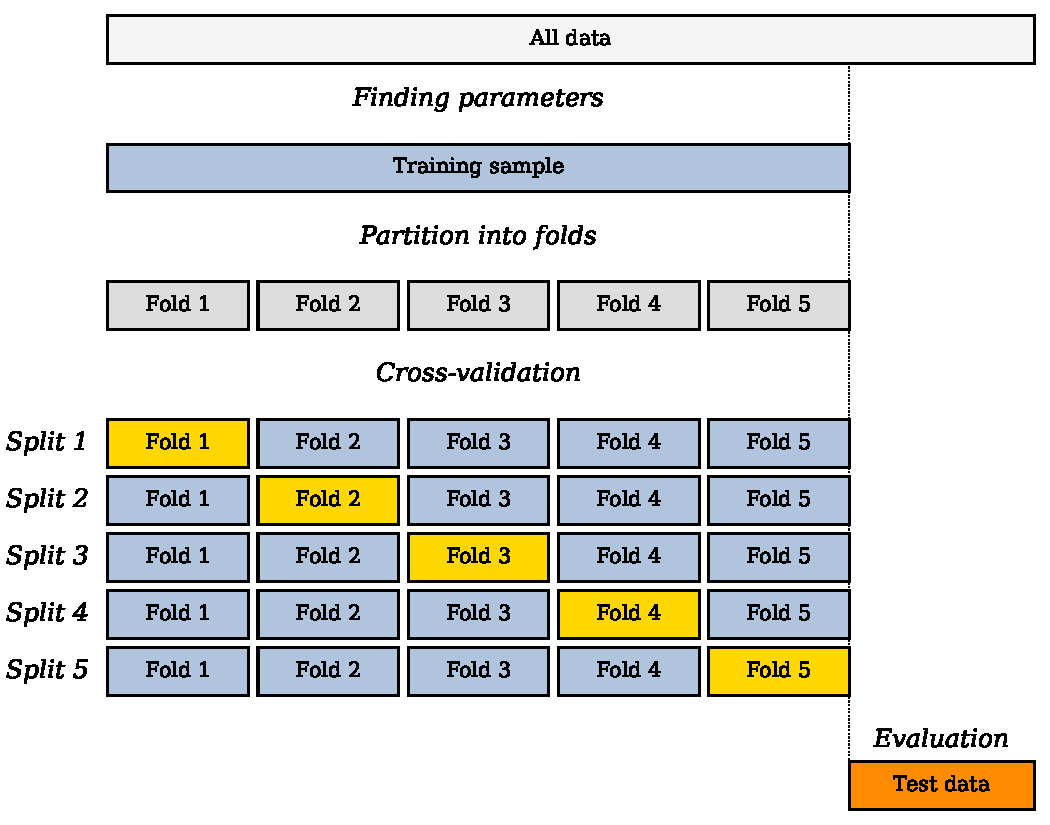
\includegraphics{images/cv_split.pdf}
\end{adjustbox}
\caption{CV split}
\end{figure}

    In this unit we will skip the final step of assessing generalisability
on the test data set. Consequently, when running cross-validation, we
will only use training/validation data sets and we will use the terms
``validation'' and ``test'' interchangeably.

The \texttt{scikit-learn}
\href{https://scikit-learn.org/stable/modules/cross_validation.html}{documentation}
contains a wealth of additional information on cross-validation. Another
method to perform hyperparameter tuning is
\href{https://scikit-learn.org/stable/modules/grid_search.html}{grid
search} which we won't cover in this unit.

    \hypertarget{examle-tuning-of-the-polynomial-degree}{%
\subsection{Examle: Tuning of the polynomial
degree}\label{examle-tuning-of-the-polynomial-degree}}

To illustrate the concept, we demonstrate the procedure outlined above
by tuning the polynomial degree for the example covered in the previous
section by minimising the root mean squared error (RMSE).

We recreate the data set in the same way as before, using
\texttt{LivingArea} and \texttt{LotArea} as explanatory variables.

    \begin{tcolorbox}[breakable, size=fbox, boxrule=1pt, pad at break*=1mm,colback=cellbackground, colframe=cellborder]
\prompt{In}{incolor}{502}{\boxspacing}
\begin{Verbatim}[commandchars=\\\{\}]
\PY{k+kn}{import} \PY{n+nn}{pandas} \PY{k}{as} \PY{n+nn}{pd}

\PY{n}{df} \PY{o}{=} \PY{n}{pd}\PY{o}{.}\PY{n}{read\PYZus{}csv}\PY{p}{(}\PY{l+s+sa}{f}\PY{l+s+s1}{\PYZsq{}}\PY{l+s+si}{\PYZob{}}\PY{n}{DATA\PYZus{}PATH}\PY{l+s+si}{\PYZcb{}}\PY{l+s+s1}{/ames\PYZus{}houses.csv}\PY{l+s+s1}{\PYZsq{}}\PY{p}{)}

\PY{n}{features} \PY{o}{=} \PY{p}{[}\PY{l+s+s1}{\PYZsq{}}\PY{l+s+s1}{LivingArea}\PY{l+s+s1}{\PYZsq{}}\PY{p}{,} \PY{l+s+s1}{\PYZsq{}}\PY{l+s+s1}{LotArea}\PY{l+s+s1}{\PYZsq{}}\PY{p}{]}
\PY{n}{target} \PY{o}{=} \PY{l+s+s1}{\PYZsq{}}\PY{l+s+s1}{SalePrice}\PY{l+s+s1}{\PYZsq{}}

\PY{n}{y} \PY{o}{=} \PY{n}{df}\PY{p}{[}\PY{n}{target}\PY{p}{]}\PY{o}{.}\PY{n}{to\PYZus{}numpy}\PY{p}{(}\PY{p}{)}
\PY{n}{X} \PY{o}{=} \PY{n}{df}\PY{p}{[}\PY{n}{features}\PY{p}{]}\PY{o}{.}\PY{n}{to\PYZus{}numpy}\PY{p}{(}\PY{p}{)}
\end{Verbatim}
\end{tcolorbox}

    We now iterate over the candidate polynomial degrees \(d = 0,\dots,4\)
and apply \(k\)-fold cross-validation with 10 folds. There is no need to
manually split the sample into training and validation/test sub-sets.
Instead, we use the
\href{https://scikit-learn.org/stable/modules/generated/sklearn.model_selection.KFold.html\#sklearn.model_selection.KFold}{\texttt{KFold}}
class to automatically create the splits for us. Once we have created an
instance with the desired number of folds, \eg
\texttt{KFold(n\_splits=10)}, we can call the \texttt{split()} method
which iterates trough all possible combinations of training and test
data sets and returns the array indices for each.

    \begin{tcolorbox}[breakable, size=fbox, boxrule=1pt, pad at break*=1mm,colback=cellbackground, colframe=cellborder]
\prompt{In}{incolor}{503}{\boxspacing}
\begin{Verbatim}[commandchars=\\\{\}]
\PY{k+kn}{from} \PY{n+nn}{sklearn}\PY{n+nn}{.}\PY{n+nn}{pipeline} \PY{k+kn}{import} \PY{n}{Pipeline}
\PY{k+kn}{from} \PY{n+nn}{sklearn}\PY{n+nn}{.}\PY{n+nn}{preprocessing} \PY{k+kn}{import} \PY{n}{PolynomialFeatures}
\PY{k+kn}{from} \PY{n+nn}{sklearn}\PY{n+nn}{.}\PY{n+nn}{linear\PYZus{}model} \PY{k+kn}{import} \PY{n}{LinearRegression}
\PY{k+kn}{from} \PY{n+nn}{sklearn}\PY{n+nn}{.}\PY{n+nn}{model\PYZus{}selection} \PY{k+kn}{import} \PY{n}{KFold}
\PY{k+kn}{from} \PY{n+nn}{sklearn}\PY{n+nn}{.}\PY{n+nn}{metrics} \PY{k+kn}{import} \PY{n}{mean\PYZus{}squared\PYZus{}error}

\PY{n}{degrees} \PY{o}{=} \PY{n}{np}\PY{o}{.}\PY{n}{arange}\PY{p}{(}\PY{l+m+mi}{5}\PY{p}{)}

\PY{n}{rmse\PYZus{}mean} \PY{o}{=} \PY{p}{[}\PY{p}{]}

\PY{k}{for} \PY{n}{d} \PY{o+ow}{in} \PY{n}{degrees}\PY{p}{:}

    \PY{c+c1}{\PYZsh{} Create pipeline to transform and fit the model. Pipeline depends}
    \PY{c+c1}{\PYZsh{} on polynomial degree!}
    \PY{n}{pipe} \PY{o}{=} \PY{n}{Pipeline}\PY{p}{(}\PY{n}{steps}\PY{o}{=}\PY{p}{[}
        \PY{p}{(}\PY{l+s+s1}{\PYZsq{}}\PY{l+s+s1}{poly}\PY{l+s+s1}{\PYZsq{}}\PY{p}{,} \PY{n}{PolynomialFeatures}\PY{p}{(}\PY{n}{degree}\PY{o}{=}\PY{n}{d}\PY{p}{,} \PY{n}{include\PYZus{}bias}\PY{o}{=}\PY{k+kc}{True}\PY{p}{)}\PY{p}{)}\PY{p}{,}
        \PY{p}{(}\PY{l+s+s1}{\PYZsq{}}\PY{l+s+s1}{lr}\PY{l+s+s1}{\PYZsq{}}\PY{p}{,} \PY{n}{LinearRegression}\PY{p}{(}\PY{n}{fit\PYZus{}intercept}\PY{o}{=}\PY{k+kc}{False}\PY{p}{)}\PY{p}{)}
    \PY{p}{]}\PY{p}{)}

    \PY{n}{rmse\PYZus{}fold} \PY{o}{=} \PY{p}{[}\PY{p}{]}

    \PY{c+c1}{\PYZsh{} Create 10 folds}
    \PY{n}{folds} \PY{o}{=} \PY{n}{KFold}\PY{p}{(}\PY{n}{n\PYZus{}splits}\PY{o}{=}\PY{l+m+mi}{10}\PY{p}{)}

    \PY{c+c1}{\PYZsh{} Iterate through all combinations of training/test data}
    \PY{k}{for} \PY{n}{itrain}\PY{p}{,} \PY{n}{itest} \PY{o+ow}{in} \PY{n}{folds}\PY{o}{.}\PY{n}{split}\PY{p}{(}\PY{n}{X}\PY{p}{,} \PY{n}{y}\PY{p}{)}\PY{p}{:}

        \PY{c+c1}{\PYZsh{} Extract training data for this split}
        \PY{n}{X\PYZus{}train} \PY{o}{=} \PY{n}{X}\PY{p}{[}\PY{n}{itrain}\PY{p}{]}
        \PY{n}{y\PYZus{}train} \PY{o}{=} \PY{n}{y}\PY{p}{[}\PY{n}{itrain}\PY{p}{]}

        \PY{c+c1}{\PYZsh{} Extract test (or validation) data for this split}
        \PY{n}{X\PYZus{}test} \PY{o}{=} \PY{n}{X}\PY{p}{[}\PY{n}{itest}\PY{p}{]}
        \PY{n}{y\PYZus{}test} \PY{o}{=} \PY{n}{y}\PY{p}{[}\PY{n}{itest}\PY{p}{]}

        \PY{c+c1}{\PYZsh{} Fit model on training data for given degree}
        \PY{n}{pipe}\PY{o}{.}\PY{n}{fit}\PY{p}{(}\PY{n}{X\PYZus{}train}\PY{p}{,} \PY{n}{y\PYZus{}train}\PY{p}{)}

        \PY{c+c1}{\PYZsh{} Predict response on test data}
        \PY{n}{y\PYZus{}test\PYZus{}hat} \PY{o}{=} \PY{n}{pipe}\PY{o}{.}\PY{n}{predict}\PY{p}{(}\PY{n}{X\PYZus{}test}\PY{p}{)}

        \PY{c+c1}{\PYZsh{} Compute RMSE as model fit measure: function returns RMSE }
        \PY{c+c1}{\PYZsh{} if squared=False is passed!}
        \PY{n}{rmse} \PY{o}{=} \PY{n}{mean\PYZus{}squared\PYZus{}error}\PY{p}{(}\PY{n}{y\PYZus{}test}\PY{p}{,} \PY{n}{y\PYZus{}test\PYZus{}hat}\PY{p}{,} \PY{n}{squared}\PY{o}{=}\PY{k+kc}{False}\PY{p}{)}

        \PY{c+c1}{\PYZsh{} Store RMSE for current split}
        \PY{n}{rmse\PYZus{}fold}\PY{o}{.}\PY{n}{append}\PY{p}{(}\PY{n}{rmse}\PY{p}{)}

    \PY{c+c1}{\PYZsh{} Store average MSE for current degree}
    \PY{n}{rmse\PYZus{}mean}\PY{o}{.}\PY{n}{append}\PY{p}{(}\PY{n}{np}\PY{o}{.}\PY{n}{mean}\PY{p}{(}\PY{n}{rmse\PYZus{}fold}\PY{p}{)}\PY{p}{)}
    
\PY{c+c1}{\PYZsh{} Convert to NumPy array}
\PY{n}{rmse\PYZus{}mean} \PY{o}{=} \PY{n}{np}\PY{o}{.}\PY{n}{array}\PY{p}{(}\PY{n}{rmse\PYZus{}mean}\PY{p}{)}

\PY{c+c1}{\PYZsh{} Print average RMSE for all polynomial degrees}
\PY{n}{rmse\PYZus{}mean}
\end{Verbatim}
\end{tcolorbox}

            \begin{tcolorbox}[breakable, size=fbox, boxrule=.5pt, pad at break*=1mm, opacityfill=0]
\prompt{Out}{outcolor}{503}{\boxspacing}
\begin{Verbatim}[commandchars=\\\{\}]
array([ 79020.25214052,  55268.49840787,  55228.58262433,  55885.05011959,
       437205.34703289])
\end{Verbatim}
\end{tcolorbox}
        
    This code returns an array of 5 averaged RMSEs, one for each
\(d = 0, \dots, 4\). We can now find the optimal \(d\) by picking the
one which has the lowest mean squared error in the test samples using
the
\href{https://numpy.org/doc/stable/reference/generated/numpy.argmin.html}{\texttt{argmin()}}
function which returns the \emph{index} of the smallest array element.

    \begin{tcolorbox}[breakable, size=fbox, boxrule=1pt, pad at break*=1mm,colback=cellbackground, colframe=cellborder]
\prompt{In}{incolor}{504}{\boxspacing}
\begin{Verbatim}[commandchars=\\\{\}]
\PY{n}{imin} \PY{o}{=} \PY{n}{np}\PY{o}{.}\PY{n}{argmin}\PY{p}{(}\PY{n}{rmse\PYZus{}mean}\PY{p}{)}
\PY{n}{dmin} \PY{o}{=} \PY{n}{degrees}\PY{p}{[}\PY{n}{imin}\PY{p}{]}

\PY{n+nb}{print}\PY{p}{(}\PY{l+s+sa}{f}\PY{l+s+s1}{\PYZsq{}}\PY{l+s+s1}{Polynomial degree with min. RMSE: }\PY{l+s+si}{\PYZob{}}\PY{n}{dmin}\PY{l+s+si}{\PYZcb{}}\PY{l+s+s1}{\PYZsq{}}\PY{p}{)}
\end{Verbatim}
\end{tcolorbox}

    \begin{Verbatim}[commandchars=\\\{\}]
Polynomial degree with min. RMSE: 2
    \end{Verbatim}

    Finally, it is often instructive how the RMSE evolves as a function of
the hyperparameter we want to tune.

    \begin{tcolorbox}[breakable, size=fbox, boxrule=1pt, pad at break*=1mm,colback=cellbackground, colframe=cellborder]
\prompt{In}{incolor}{505}{\boxspacing}
\begin{Verbatim}[commandchars=\\\{\}]
\PY{n}{plt}\PY{o}{.}\PY{n}{plot}\PY{p}{(}\PY{n}{degrees}\PY{p}{,} \PY{n}{rmse\PYZus{}mean}\PY{p}{,} \PY{n}{marker}\PY{o}{=}\PY{l+s+s1}{\PYZsq{}}\PY{l+s+s1}{o}\PY{l+s+s1}{\PYZsq{}}\PY{p}{,} \PY{n}{ms}\PY{o}{=}\PY{l+m+mi}{3}\PY{p}{)}
\PY{n}{plt}\PY{o}{.}\PY{n}{xlabel}\PY{p}{(}\PY{l+s+s1}{\PYZsq{}}\PY{l+s+s1}{Polynomial degree}\PY{l+s+s1}{\PYZsq{}}\PY{p}{)}
\PY{n}{plt}\PY{o}{.}\PY{n}{ylabel}\PY{p}{(}\PY{l+s+s1}{\PYZsq{}}\PY{l+s+s1}{Cross\PYZhy{}validated RMSE}\PY{l+s+s1}{\PYZsq{}}\PY{p}{)}
\PY{n}{plt}\PY{o}{.}\PY{n}{scatter}\PY{p}{(}\PY{n}{degrees}\PY{p}{[}\PY{n}{imin}\PY{p}{]}\PY{p}{,} \PY{n}{rmse\PYZus{}mean}\PY{p}{[}\PY{n}{imin}\PY{p}{]}\PY{p}{,} \PY{n}{s}\PY{o}{=}\PY{l+m+mi}{15}\PY{p}{,} \PY{n}{c}\PY{o}{=}\PY{l+s+s1}{\PYZsq{}}\PY{l+s+s1}{black}\PY{l+s+s1}{\PYZsq{}}\PY{p}{,} \PY{n}{zorder}\PY{o}{=}\PY{l+m+mi}{100}\PY{p}{)}
\PY{n}{plt}\PY{o}{.}\PY{n}{xticks}\PY{p}{(}\PY{n}{degrees}\PY{p}{)}
\PY{n}{plt}\PY{o}{.}\PY{n}{axvline}\PY{p}{(}\PY{n}{imin}\PY{p}{,} \PY{n}{ls}\PY{o}{=}\PY{l+s+s1}{\PYZsq{}}\PY{l+s+s1}{:}\PY{l+s+s1}{\PYZsq{}}\PY{p}{,} \PY{n}{lw}\PY{o}{=}\PY{l+m+mf}{0.75}\PY{p}{,} \PY{n}{c}\PY{o}{=}\PY{l+s+s1}{\PYZsq{}}\PY{l+s+s1}{black}\PY{l+s+s1}{\PYZsq{}}\PY{p}{)}
\end{Verbatim}
\end{tcolorbox}

            \begin{tcolorbox}[breakable, size=fbox, boxrule=.5pt, pad at break*=1mm, opacityfill=0]
\prompt{Out}{outcolor}{505}{\boxspacing}
\begin{Verbatim}[commandchars=\\\{\}]
<matplotlib.lines.Line2D at 0x7fd00da0e920>
\end{Verbatim}
\end{tcolorbox}
        
    \begin{center}
    \adjustimage{max size={0.9\linewidth}{0.9\paperheight}}{MLFP-part1_files/MLFP-part1_1047_1.pdf}
    \end{center}
    
    Here we see that for \(d=0\) (the intercept-only model), the model
underfits the data leading to a high prediction error. However, higher
\(d\)'s do not always translate into a better fit. For \(d = 4\), the
model vastly overfits the data, resulting in poor performance in the
test sample and a very large RMSE.

    \hypertarget{automating-cross-validation}{%
\subsubsection{Automating
cross-validation}\label{automating-cross-validation}}

The code implemented above to run cross-validation was needlessly
complex even though we leveraged the \texttt{KFold} class to do the
sample splitting for us. Fortunately, \texttt{scikit-learn} provides us
with even more convenience functions that further simplify this process.
For example, if we want to perform tuning based on a single score (such
as the root mean squared error), we can instead use
\href{https://scikit-learn.org/stable/modules/generated/sklearn.model_selection.cross_val_score.html}{\texttt{cross\_val\_score()}}.
This function requires us to specify an estimator (or a pipeline), the
number of folds to use for cross-validation (\texttt{cv=10}) and the
metric to evaluate. For example, if we want to compute the RMSE, we
would pass the argument
\texttt{scoring=\textquotesingle{}neg\_root\_mean\_squared\_error\textquotesingle{}}.
Note that the function returns the \emph{negative} RMSE which we need to
correct manually.

See the
\href{https://scikit-learn.org/stable/modules/model_evaluation.html\#scoring-parameter}{documentation}
for a complete list of valid metrics that can be passed as
\texttt{scoring} arguments. Alternatively, \texttt{scikit-learn} lists
available metrics by running

\begin{Shaded}
\begin{Highlighting}[]
\ImportTok{import}\NormalTok{ sklearn.metrics}
\NormalTok{sklearn.metrics.get\_scorer\_names()}
\end{Highlighting}
\end{Shaded}

The following code re-implements the k-fold cross-validation from
earlier using \texttt{cross\_val\_score()}:

    \begin{tcolorbox}[breakable, size=fbox, boxrule=1pt, pad at break*=1mm,colback=cellbackground, colframe=cellborder]
\prompt{In}{incolor}{506}{\boxspacing}
\begin{Verbatim}[commandchars=\\\{\}]
\PY{k+kn}{from} \PY{n+nn}{sklearn}\PY{n+nn}{.}\PY{n+nn}{model\PYZus{}selection} \PY{k+kn}{import} \PY{n}{cross\PYZus{}val\PYZus{}score}

\PY{n}{degrees} \PY{o}{=} \PY{n}{np}\PY{o}{.}\PY{n}{arange}\PY{p}{(}\PY{l+m+mi}{5}\PY{p}{)}

\PY{n}{rmse\PYZus{}mean} \PY{o}{=} \PY{p}{[}\PY{p}{]}
\PY{n}{rmse\PYZus{}std} \PY{o}{=} \PY{p}{[}\PY{p}{]}

\PY{k}{for} \PY{n}{d} \PY{o+ow}{in} \PY{n}{degrees}\PY{p}{:}

    \PY{n}{pipe} \PY{o}{=} \PY{n}{Pipeline}\PY{p}{(}\PY{n}{steps}\PY{o}{=}\PY{p}{[}
        \PY{p}{(}\PY{l+s+s1}{\PYZsq{}}\PY{l+s+s1}{poly}\PY{l+s+s1}{\PYZsq{}}\PY{p}{,} \PY{n}{PolynomialFeatures}\PY{p}{(}\PY{n}{degree}\PY{o}{=}\PY{n}{d}\PY{p}{,} \PY{n}{include\PYZus{}bias}\PY{o}{=}\PY{k+kc}{True}\PY{p}{)}\PY{p}{)}\PY{p}{,}
        \PY{p}{(}\PY{l+s+s1}{\PYZsq{}}\PY{l+s+s1}{lr}\PY{l+s+s1}{\PYZsq{}}\PY{p}{,} \PY{n}{LinearRegression}\PY{p}{(}\PY{n}{fit\PYZus{}intercept}\PY{o}{=}\PY{k+kc}{False}\PY{p}{)}\PY{p}{)}
    \PY{p}{]}\PY{p}{)}

    \PY{n}{score} \PY{o}{=} \PY{n}{cross\PYZus{}val\PYZus{}score}\PY{p}{(}
        \PY{n}{pipe}\PY{p}{,} 
        \PY{n}{X}\PY{p}{,} \PY{n}{y}\PY{p}{,} 
        \PY{n}{scoring}\PY{o}{=}\PY{l+s+s1}{\PYZsq{}}\PY{l+s+s1}{neg\PYZus{}root\PYZus{}mean\PYZus{}squared\PYZus{}error}\PY{l+s+s1}{\PYZsq{}}\PY{p}{,} 
        \PY{n}{cv}\PY{o}{=}\PY{l+m+mi}{10}
    \PY{p}{)}

    \PY{c+c1}{\PYZsh{} Function returns NEGATIVE RMSE, correct this here!}
    \PY{n}{rmse\PYZus{}mean}\PY{o}{.}\PY{n}{append}\PY{p}{(}\PY{n}{np}\PY{o}{.}\PY{n}{mean}\PY{p}{(}\PY{o}{\PYZhy{}}\PY{n}{score}\PY{p}{)}\PY{p}{)}
    \PY{c+c1}{\PYZsh{} Compute std. dev. of RMSE across splits}
    \PY{n}{rmse\PYZus{}std}\PY{o}{.}\PY{n}{append}\PY{p}{(}\PY{n}{np}\PY{o}{.}\PY{n}{std}\PY{p}{(}\PY{o}{\PYZhy{}}\PY{n}{score}\PY{p}{)}\PY{p}{)}
    
\PY{c+c1}{\PYZsh{} Convert to NumPy array}
\PY{n}{rmse\PYZus{}mean} \PY{o}{=} \PY{n}{np}\PY{o}{.}\PY{n}{array}\PY{p}{(}\PY{n}{rmse\PYZus{}mean}\PY{p}{)}
\PY{n}{rmse\PYZus{}std} \PY{o}{=} \PY{n}{np}\PY{o}{.}\PY{n}{array}\PY{p}{(}\PY{n}{rmse\PYZus{}std}\PY{p}{)}

\PY{c+c1}{\PYZsh{} Print average RMSE for all polynomial degrees}
\PY{n}{rmse\PYZus{}mean}
\end{Verbatim}
\end{tcolorbox}

            \begin{tcolorbox}[breakable, size=fbox, boxrule=.5pt, pad at break*=1mm, opacityfill=0]
\prompt{Out}{outcolor}{506}{\boxspacing}
\begin{Verbatim}[commandchars=\\\{\}]
array([ 79020.25214052,  55268.49840787,  55228.58262433,  55885.05011959,
       437205.34703289])
\end{Verbatim}
\end{tcolorbox}
        
    The RMSE-minimising degree is of course the same as before:

    \begin{tcolorbox}[breakable, size=fbox, boxrule=1pt, pad at break*=1mm,colback=cellbackground, colframe=cellborder]
\prompt{In}{incolor}{507}{\boxspacing}
\begin{Verbatim}[commandchars=\\\{\}]
\PY{n}{imin} \PY{o}{=} \PY{n}{np}\PY{o}{.}\PY{n}{argmin}\PY{p}{(}\PY{n}{rmse\PYZus{}mean}\PY{p}{)}
\PY{n}{dmin} \PY{o}{=} \PY{n}{degrees}\PY{p}{[}\PY{n}{imin}\PY{p}{]}

\PY{n+nb}{print}\PY{p}{(}\PY{l+s+sa}{f}\PY{l+s+s1}{\PYZsq{}}\PY{l+s+s1}{Polynomial degree with min. RMSE: }\PY{l+s+si}{\PYZob{}}\PY{n}{dmin}\PY{l+s+si}{\PYZcb{}}\PY{l+s+s1}{\PYZsq{}}\PY{p}{)}
\end{Verbatim}
\end{tcolorbox}

    \begin{Verbatim}[commandchars=\\\{\}]
Polynomial degree with min. RMSE: 2
    \end{Verbatim}


\hypertarget{linear-models-with-regularisation-ridge-regression}{%
\section{Linear models with regularisation: Ridge
regression}\label{linear-models-with-regularisation-ridge-regression}}

The linear models we encountered so far are part of the standard
econometrics toolbox. In this section, we look at extensions that make
these models more useful for machine learning applications.

The first model we study is Ridge regression, which estimates a linear
model but adds a penalty term to the loss function which is now given by
\[
L(\mu, \bm\beta) = 
    \underbrace{\sum_{i=1}^N \Bigl(
    y_i - \mu - \mathbf{x}_i'\bm\beta\Bigr)^2}_{\text{Sum of squared errors}}
    + 
    \underbrace{\alpha \sum_{k=1}^K\beta_k^2}_{\text{L2 penalty}}
\] Compared to ordinary least squares (OLS) we discussed initially, the
penalty term increases the loss function if the estimated coefficients
\(\bm\beta\) are large. This term is called an L2 penalty because
it corresponds to the (squared) L2 vector norm. In many textbooks, you
will see the penalty term written as \(\alpha \|\bm\beta\|_2^2\)
which is equivalent to the formula used above.

For any \(\alpha > 0\), the loss function is increasing in the
(absolute) coefficient values, thus the minimum \(L\) might be one where
the elements of \(\bm\beta\) are smaller than what they would have
been with OLS. We therefore say that that Ridge regression applies
\emph{regularisation} or \emph{shrinkage}. Note, however, that the
intercept which we now denote by \(\mu\) is not included in the penalty
term, and thus no regularisation is applied to it.

Clearly, the regularisation strength depends on the value of \(\alpha\).
For tiny (or zero) \(\alpha\), the estimated
\(\widehat{\bm\beta}\) will be close (or identical) to OLS, while
for large \(\alpha\) the estimated coefficients will be compressed
towards zero. In this setting, \(\alpha\) is a hyperparameter and we can
accordingly use cross-validation to find an ``optimal'' value.

Why would we ever want to use Ridge regression given that OLS is the
best linear unbiased estimator? It turns out that regularisation can
help in scenarios where we have a large number of (potentially
multicollinear) regressors in which case OLS is prone to overfitting.

    \hypertarget{example-polynomial-approximation}{%
\subsection{Example: Polynomial
approximation}\label{example-polynomial-approximation}}

We illustrate such problems and the benefits of Ridge regression using a
highly stylised example. Imagine we want to approximate a non-linear
function using a high-order polynomial, a setting which is notoriously
susceptible to overfitting (also see the optional exercises for more
illustrations). Assume that our model is given by \[
\begin{aligned}
y_i &= \cos\left( \frac{3}{2}\pi x_i \right) + \epsilon_i \\
    \epsilon &\stackrel{\text{iid}}{\sim} N(0, 0.25)
\end{aligned}
\] where \(\epsilon_i\) as an additive, normally-distributed measurement
error term with mean \(0\) and variance \(\frac{1}{4}\).

The following code creates and plots a demo sample with \(N=100\)
observations. The true values of \(y\) (without measurement error) are
computed using the function \texttt{compute\_true\_y()} which returns
\(y\) for a given \(x\).

    \begin{tcolorbox}[breakable, size=fbox, boxrule=1pt, pad at break*=1mm,colback=cellbackground, colframe=cellborder]
\prompt{In}{incolor}{508}{\boxspacing}
\begin{Verbatim}[commandchars=\\\{\}]
\PY{k+kn}{import} \PY{n+nn}{numpy} \PY{k}{as} \PY{n+nn}{np}
\PY{k+kn}{from} \PY{n+nn}{numpy}\PY{n+nn}{.}\PY{n+nn}{random} \PY{k+kn}{import} \PY{n}{default\PYZus{}rng}

\PY{c+c1}{\PYZsh{} Initialise random number generator}
\PY{n}{rng} \PY{o}{=} \PY{n}{default\PYZus{}rng}\PY{p}{(}\PY{l+m+mi}{1234}\PY{p}{)}

\PY{c+c1}{\PYZsh{} Sample size}
\PY{n}{N} \PY{o}{=} \PY{l+m+mi}{100}

\PY{c+c1}{\PYZsh{} True function (w/o errors)}
\PY{k}{def} \PY{n+nf}{compute\PYZus{}true\PYZus{}y}\PY{p}{(}\PY{n}{x}\PY{p}{)}\PY{p}{:}
    \PY{k}{return} \PY{n}{np}\PY{o}{.}\PY{n}{cos}\PY{p}{(}\PY{l+m+mf}{1.5} \PY{o}{*} \PY{n}{np}\PY{o}{.}\PY{n}{pi} \PY{o}{*} \PY{n}{x}\PY{p}{)}

\PY{c+c1}{\PYZsh{} Randomly draw explanatory variable x uniformly distributed on [0, 1]}
\PY{n}{x} \PY{o}{=} \PY{n}{rng}\PY{o}{.}\PY{n}{random}\PY{p}{(}\PY{n}{size}\PY{o}{=}\PY{n}{N}\PY{p}{)}

\PY{c+c1}{\PYZsh{} Draw errors from normal distribution}
\PY{n}{epsilon} \PY{o}{=} \PY{n}{rng}\PY{o}{.}\PY{n}{normal}\PY{p}{(}\PY{n}{scale}\PY{o}{=}\PY{l+m+mf}{0.5}\PY{p}{,} \PY{n}{size}\PY{o}{=}\PY{n}{N}\PY{p}{)}

\PY{c+c1}{\PYZsh{} Compute y, add measurement error}
\PY{n}{y} \PY{o}{=} \PY{n}{compute\PYZus{}true\PYZus{}y}\PY{p}{(}\PY{n}{x}\PY{p}{)} \PY{o}{+} \PY{n}{epsilon}
\end{Verbatim}
\end{tcolorbox}

    The next graph visualises the true relationship and the sample points
\((x_i, y_i)\).

    \begin{tcolorbox}[breakable, size=fbox, boxrule=1pt, pad at break*=1mm,colback=cellbackground, colframe=cellborder]
\prompt{In}{incolor}{509}{\boxspacing}
\begin{Verbatim}[commandchars=\\\{\}]
\PY{k+kn}{import} \PY{n+nn}{matplotlib}\PY{n+nn}{.}\PY{n+nn}{pyplot} \PY{k}{as} \PY{n+nn}{plt}


\PY{n}{xvalues} \PY{o}{=} \PY{n}{np}\PY{o}{.}\PY{n}{linspace}\PY{p}{(}\PY{l+m+mf}{0.0}\PY{p}{,} \PY{l+m+mf}{1.0}\PY{p}{,} \PY{l+m+mi}{101}\PY{p}{)}
\PY{n}{plt}\PY{o}{.}\PY{n}{plot}\PY{p}{(}\PY{n}{xvalues}\PY{p}{,} \PY{n}{compute\PYZus{}true\PYZus{}y}\PY{p}{(}\PY{n}{xvalues}\PY{p}{)}\PY{p}{,} \PY{n}{color}\PY{o}{=}\PY{l+s+s1}{\PYZsq{}}\PY{l+s+s1}{black}\PY{l+s+s1}{\PYZsq{}}\PY{p}{,} \PY{n}{lw}\PY{o}{=}\PY{l+m+mf}{1.0}\PY{p}{,} 
    \PY{n}{label}\PY{o}{=}\PY{l+s+s1}{\PYZsq{}}\PY{l+s+s1}{True function}\PY{l+s+s1}{\PYZsq{}}\PY{p}{)}
\PY{n}{plt}\PY{o}{.}\PY{n}{scatter}\PY{p}{(}\PY{n}{x}\PY{p}{,} \PY{n}{y}\PY{p}{,} \PY{n}{s}\PY{o}{=}\PY{l+m+mi}{20}\PY{p}{,} \PY{n}{color}\PY{o}{=}\PY{l+s+s1}{\PYZsq{}}\PY{l+s+s1}{none}\PY{l+s+s1}{\PYZsq{}}\PY{p}{,} \PY{n}{edgecolor}\PY{o}{=}\PY{l+s+s1}{\PYZsq{}}\PY{l+s+s1}{steelblue}\PY{l+s+s1}{\PYZsq{}}\PY{p}{,} 
    \PY{n}{lw}\PY{o}{=}\PY{l+m+mf}{0.75}\PY{p}{,} \PY{n}{label}\PY{o}{=}\PY{l+s+s1}{\PYZsq{}}\PY{l+s+s1}{Sample}\PY{l+s+s1}{\PYZsq{}}\PY{p}{)}
\PY{n}{plt}\PY{o}{.}\PY{n}{xlabel}\PY{p}{(}\PY{l+s+s1}{\PYZsq{}}\PY{l+s+s1}{\PYZdl{}x\PYZdl{}}\PY{l+s+s1}{\PYZsq{}}\PY{p}{)}
\PY{n}{plt}\PY{o}{.}\PY{n}{ylabel}\PY{p}{(}\PY{l+s+s1}{\PYZsq{}}\PY{l+s+s1}{\PYZdl{}y\PYZdl{}}\PY{l+s+s1}{\PYZsq{}}\PY{p}{)}
\end{Verbatim}
\end{tcolorbox}

            \begin{tcolorbox}[breakable, size=fbox, boxrule=.5pt, pad at break*=1mm, opacityfill=0]
\prompt{Out}{outcolor}{509}{\boxspacing}
\begin{Verbatim}[commandchars=\\\{\}]
Text(0, 0.5, '\$y\$')
\end{Verbatim}
\end{tcolorbox}
        
    \begin{center}
    \adjustimage{max size={0.9\linewidth}{0.9\paperheight}}{MLFP-part1_files/MLFP-part1_1057_1.pdf}
    \end{center}
    
    \hypertarget{estimating-the-ridge-and-linear-regression-models}{%
\subsubsection{Estimating the Ridge and linear regression
models}\label{estimating-the-ridge-and-linear-regression-models}}

We now estimate a polynomial approximation where we assume that \(y\) is
a degree-\(K\) polynomial in \(x\), \ie \[
y_i \approx \mu + \beta_1 x_i + \beta_2 x_i^2 + \cdots + \beta_K x_i^K 
\] For this example, we choose an unconventionally high \(K=15\) since
we anticipate that this leads to problems with OLS.

A few more steps are required before we can run the Ridge regression:

\begin{itemize}
\tightlist
\item
  We need to create the polynomial in \(x\) which we do with the
  \href{https://scikit-learn.org/stable/modules/generated/sklearn.preprocessing.PolynomialFeatures.html}{\texttt{PolynomialFeatures}}
  transformation we already encountered.
\item
  Moreover, regularisation methods can be susceptible to scaling issues,
  so we need to demean and normalise all input variables, \ie we make
  sure that each feature has mean \(0\) and a variance of \(1\). We can
  automate this step using the
  \href{https://scikit-learn.org/stable/modules/generated/sklearn.preprocessing.StandardScaler.html}{\texttt{StandardScaler}}
  transformation.
\item
  Finally, we build a
  \href{https://scikit-learn.org/stable/modules/generated/sklearn.pipeline.Pipeline.html}{\texttt{Pipeline}}
  that combines these transformation together with the final estimation
  step. We use the function
  \href{https://scikit-learn.org/stable/modules/generated/sklearn.pipeline.make_pipeline.html}{\texttt{make\_pipeline()}}
  to simplify this step.
\end{itemize}

To run the Ridge regression, we moreover need to specify the
regularisation strength \(\alpha\) which we set to \(\alpha = 3\) for
illustration.

    \begin{tcolorbox}[breakable, size=fbox, boxrule=1pt, pad at break*=1mm,colback=cellbackground, colframe=cellborder]
\prompt{In}{incolor}{510}{\boxspacing}
\begin{Verbatim}[commandchars=\\\{\}]
\PY{k+kn}{from} \PY{n+nn}{sklearn}\PY{n+nn}{.}\PY{n+nn}{linear\PYZus{}model} \PY{k+kn}{import} \PY{n}{Ridge}
\PY{k+kn}{from} \PY{n+nn}{sklearn}\PY{n+nn}{.}\PY{n+nn}{preprocessing} \PY{k+kn}{import} \PY{n}{PolynomialFeatures}\PY{p}{,} \PY{n}{StandardScaler}
\PY{k+kn}{from} \PY{n+nn}{sklearn}\PY{n+nn}{.}\PY{n+nn}{pipeline} \PY{k+kn}{import} \PY{n}{make\PYZus{}pipeline}

\PY{c+c1}{\PYZsh{} Polynomial degree}
\PY{n}{degree} \PY{o}{=} \PY{l+m+mi}{15}

\PY{c+c1}{\PYZsh{} Build pipeline of transformations and Ridge estimation.}
\PY{c+c1}{\PYZsh{} We create the polynomial transformation w/o the intercept so we }
\PY{c+c1}{\PYZsh{} need to include an intercept in the fitting step.}
\PY{n}{pipe\PYZus{}ridge} \PY{o}{=} \PY{n}{make\PYZus{}pipeline}\PY{p}{(}
    \PY{n}{PolynomialFeatures}\PY{p}{(}\PY{n}{degree}\PY{o}{=}\PY{n}{degree}\PY{p}{,} \PY{n}{include\PYZus{}bias}\PY{o}{=}\PY{k+kc}{False}\PY{p}{)}\PY{p}{,}
    \PY{n}{StandardScaler}\PY{p}{(}\PY{p}{)}\PY{p}{,}
    \PY{n}{Ridge}\PY{p}{(}\PY{n}{alpha}\PY{o}{=}\PY{l+m+mf}{3.0}\PY{p}{,} \PY{n}{fit\PYZus{}intercept}\PY{o}{=}\PY{k+kc}{True}\PY{p}{)}
\PY{p}{)}

\PY{n}{pipe\PYZus{}ridge}\PY{o}{.}\PY{n}{fit}\PY{p}{(}\PY{n}{x}\PY{p}{[}\PY{p}{:}\PY{p}{,} \PY{k+kc}{None}\PY{p}{]}\PY{p}{,} \PY{n}{y}\PY{p}{)}
\end{Verbatim}
\end{tcolorbox}

            \begin{tcolorbox}[breakable, size=fbox, boxrule=.5pt, pad at break*=1mm, opacityfill=0]
\prompt{Out}{outcolor}{510}{\boxspacing}
\begin{Verbatim}[commandchars=\\\{\}]
Pipeline(steps=[('polynomialfeatures',
                 PolynomialFeatures(degree=15, include\_bias=False)),
                ('standardscaler', StandardScaler()),
                ('ridge', Ridge(alpha=3.0))])
\end{Verbatim}
\end{tcolorbox}
        
    It is instructive to estimate the same model using linear regression and
compare the results:

    \begin{tcolorbox}[breakable, size=fbox, boxrule=1pt, pad at break*=1mm,colback=cellbackground, colframe=cellborder]
\prompt{In}{incolor}{511}{\boxspacing}
\begin{Verbatim}[commandchars=\\\{\}]
\PY{k+kn}{from} \PY{n+nn}{sklearn}\PY{n+nn}{.}\PY{n+nn}{linear\PYZus{}model} \PY{k+kn}{import} \PY{n}{LinearRegression}

\PY{c+c1}{\PYZsh{} Create pipeline for linear model (linear regression does not require}
\PY{c+c1}{\PYZsh{} standardisation!)}
\PY{n}{pipe\PYZus{}lr} \PY{o}{=} \PY{n}{make\PYZus{}pipeline}\PY{p}{(}
    \PY{n}{PolynomialFeatures}\PY{p}{(}\PY{n}{degree}\PY{o}{=}\PY{n}{degree}\PY{p}{,} \PY{n}{include\PYZus{}bias}\PY{o}{=}\PY{k+kc}{False}\PY{p}{)}\PY{p}{,}
    \PY{n}{LinearRegression}\PY{p}{(}\PY{n}{fit\PYZus{}intercept}\PY{o}{=}\PY{k+kc}{True}\PY{p}{)}
\PY{p}{)}

\PY{n}{pipe\PYZus{}lr}\PY{o}{.}\PY{n}{fit}\PY{p}{(}\PY{n}{x}\PY{p}{[}\PY{p}{:}\PY{p}{,} \PY{k+kc}{None}\PY{p}{]}\PY{p}{,} \PY{n}{y}\PY{p}{)}
\end{Verbatim}
\end{tcolorbox}

            \begin{tcolorbox}[breakable, size=fbox, boxrule=.5pt, pad at break*=1mm, opacityfill=0]
\prompt{Out}{outcolor}{511}{\boxspacing}
\begin{Verbatim}[commandchars=\\\{\}]
Pipeline(steps=[('polynomialfeatures',
                 PolynomialFeatures(degree=15, include\_bias=False)),
                ('linearregression', LinearRegression())])
\end{Verbatim}
\end{tcolorbox}
        
    To illustrate the difference for this artificial example, we add the
model predictions from the Ridge and linear regressions to the sample
scatter plot we created earlier.

    \begin{tcolorbox}[breakable, size=fbox, boxrule=1pt, pad at break*=1mm,colback=cellbackground, colframe=cellborder]
\prompt{In}{incolor}{512}{\boxspacing}
\begin{Verbatim}[commandchars=\\\{\}]
\PY{k+kn}{import} \PY{n+nn}{matplotlib}\PY{n+nn}{.}\PY{n+nn}{pyplot} \PY{k}{as} \PY{n+nn}{plt}

\PY{n}{fig}\PY{p}{,} \PY{n}{ax} \PY{o}{=} \PY{n}{plt}\PY{o}{.}\PY{n}{subplots}\PY{p}{(}\PY{l+m+mi}{1}\PY{p}{,} \PY{l+m+mi}{1}\PY{p}{,} \PY{n}{figsize}\PY{o}{=}\PY{p}{(}\PY{l+m+mi}{6}\PY{p}{,} \PY{l+m+mi}{4}\PY{p}{)}\PY{p}{)}

\PY{c+c1}{\PYZsh{} Grid on which to evaluate true model and predictions}
\PY{n}{xvalues} \PY{o}{=} \PY{n}{np}\PY{o}{.}\PY{n}{linspace}\PY{p}{(}\PY{n}{np}\PY{o}{.}\PY{n}{amin}\PY{p}{(}\PY{n}{x}\PY{p}{)}\PY{p}{,} \PY{n}{np}\PY{o}{.}\PY{n}{amax}\PY{p}{(}\PY{n}{x}\PY{p}{)}\PY{p}{,} \PY{l+m+mi}{500}\PY{p}{)}

\PY{c+c1}{\PYZsh{} Sample points scatter plot}
\PY{n}{ax}\PY{o}{.}\PY{n}{scatter}\PY{p}{(}\PY{n}{x}\PY{p}{,} \PY{n}{y}\PY{p}{,} \PY{n}{s}\PY{o}{=}\PY{l+m+mi}{20}\PY{p}{,} \PY{n}{color}\PY{o}{=}\PY{l+s+s1}{\PYZsq{}}\PY{l+s+s1}{none}\PY{l+s+s1}{\PYZsq{}}\PY{p}{,} \PY{n}{edgecolor}\PY{o}{=}\PY{l+s+s1}{\PYZsq{}}\PY{l+s+s1}{steelblue}\PY{l+s+s1}{\PYZsq{}}\PY{p}{,} 
    \PY{n}{lw}\PY{o}{=}\PY{l+m+mf}{0.75}\PY{p}{,} \PY{n}{alpha}\PY{o}{=}\PY{l+m+mf}{0.7}\PY{p}{,} \PY{n}{label}\PY{o}{=}\PY{l+s+s1}{\PYZsq{}}\PY{l+s+s1}{Sample}\PY{l+s+s1}{\PYZsq{}}\PY{p}{)}

\PY{c+c1}{\PYZsh{} True model}
\PY{n}{ax}\PY{o}{.}\PY{n}{plot}\PY{p}{(}\PY{n}{xvalues}\PY{p}{,} \PY{n}{compute\PYZus{}true\PYZus{}y}\PY{p}{(}\PY{n}{xvalues}\PY{p}{)}\PY{p}{,} \PY{n}{color}\PY{o}{=}\PY{l+s+s1}{\PYZsq{}}\PY{l+s+s1}{black}\PY{l+s+s1}{\PYZsq{}}\PY{p}{,} \PY{n}{lw}\PY{o}{=}\PY{l+m+mf}{1.0}\PY{p}{,} \PY{n}{alpha}\PY{o}{=}\PY{l+m+mf}{0.9}\PY{p}{,} 
    \PY{n}{label}\PY{o}{=}\PY{l+s+s1}{\PYZsq{}}\PY{l+s+s1}{True function}\PY{l+s+s1}{\PYZsq{}}\PY{p}{)}

\PY{c+c1}{\PYZsh{} LR prediction}
\PY{n}{ax}\PY{o}{.}\PY{n}{plot}\PY{p}{(}\PY{n}{xvalues}\PY{p}{,} \PY{n}{pipe\PYZus{}lr}\PY{o}{.}\PY{n}{predict}\PY{p}{(}\PY{n}{xvalues}\PY{p}{[}\PY{p}{:}\PY{p}{,} \PY{k+kc}{None}\PY{p}{]}\PY{p}{)}\PY{p}{,} \PY{n}{color}\PY{o}{=}\PY{l+s+s1}{\PYZsq{}}\PY{l+s+s1}{purple}\PY{l+s+s1}{\PYZsq{}}\PY{p}{,} 
    \PY{n}{alpha}\PY{o}{=}\PY{l+m+mf}{0.7}\PY{p}{,} \PY{n}{label}\PY{o}{=}\PY{l+s+s1}{\PYZsq{}}\PY{l+s+s1}{Linear regression}\PY{l+s+s1}{\PYZsq{}}\PY{p}{)}

\PY{c+c1}{\PYZsh{} Ridge prediction}
\PY{n}{ax}\PY{o}{.}\PY{n}{plot}\PY{p}{(}\PY{n}{xvalues}\PY{p}{,} \PY{n}{pipe\PYZus{}ridge}\PY{o}{.}\PY{n}{predict}\PY{p}{(}\PY{n}{xvalues}\PY{p}{[}\PY{p}{:}\PY{p}{,} \PY{k+kc}{None}\PY{p}{]}\PY{p}{)}\PY{p}{,} \PY{n}{color}\PY{o}{=}\PY{l+s+s1}{\PYZsq{}}\PY{l+s+s1}{darkorange}\PY{l+s+s1}{\PYZsq{}}\PY{p}{,} \PY{n}{lw}\PY{o}{=}\PY{l+m+mf}{2.0}\PY{p}{,} 
    \PY{n}{label}\PY{o}{=}\PY{l+s+s1}{\PYZsq{}}\PY{l+s+s1}{Ridge}\PY{l+s+s1}{\PYZsq{}}\PY{p}{)}
\PY{n}{ax}\PY{o}{.}\PY{n}{legend}\PY{p}{(}\PY{p}{)}
\PY{n}{ax}\PY{o}{.}\PY{n}{set\PYZus{}xlabel}\PY{p}{(}\PY{l+s+s1}{\PYZsq{}}\PY{l+s+s1}{\PYZdl{}x\PYZdl{}}\PY{l+s+s1}{\PYZsq{}}\PY{p}{)}
\PY{n}{ax}\PY{o}{.}\PY{n}{set\PYZus{}ylabel}\PY{p}{(}\PY{l+s+s1}{\PYZsq{}}\PY{l+s+s1}{\PYZdl{}y\PYZdl{}, \PYZdl{}}\PY{l+s+s1}{\PYZbs{}}\PY{l+s+s1}{widehat}\PY{l+s+si}{\PYZob{}y\PYZcb{}}\PY{l+s+s1}{\PYZdl{}}\PY{l+s+s1}{\PYZsq{}}\PY{p}{)}
\end{Verbatim}
\end{tcolorbox}

            \begin{tcolorbox}[breakable, size=fbox, boxrule=.5pt, pad at break*=1mm, opacityfill=0]
\prompt{Out}{outcolor}{512}{\boxspacing}
\begin{Verbatim}[commandchars=\\\{\}]
Text(0, 0.5, '\$y\$, \$\textbackslash{}\textbackslash{}widehat\{y\}\$')
\end{Verbatim}
\end{tcolorbox}
        
    \begin{center}
    \adjustimage{max size={0.9\linewidth}{0.9\paperheight}}{MLFP-part1_files/MLFP-part1_1063_1.pdf}
    \end{center}
    
    As the graph shows, the OLS model vastly overfits the data which is what
we would expect in this settings. Conversely, the prediction of the
Ridge regression is reasonably close to the true function and much
better behaved despite the high polynomial degree used here.

To gain some intuition for what is going on, it is instructive to plot
the estimated Ridge coefficients for a whole range of \(\alpha\) values
which we do in the code below. Note that we choose the grid of
\(\alpha\) to be uniformly spaced in logs since we want to zoom in on
what happens when \(\alpha\) is small.

    \begin{tcolorbox}[breakable, size=fbox, boxrule=1pt, pad at break*=1mm,colback=cellbackground, colframe=cellborder]
\prompt{In}{incolor}{513}{\boxspacing}
\begin{Verbatim}[commandchars=\\\{\}]
\PY{c+c1}{\PYZsh{} Create grid of alphas spaced uniformly in logs}
\PY{n}{alphas} \PY{o}{=} \PY{n}{np}\PY{o}{.}\PY{n}{logspace}\PY{p}{(}\PY{n}{np}\PY{o}{.}\PY{n}{log10}\PY{p}{(}\PY{l+m+mf}{5.0e\PYZhy{}3}\PY{p}{)}\PY{p}{,} \PY{n}{np}\PY{o}{.}\PY{n}{log10}\PY{p}{(}\PY{l+m+mf}{1000.0}\PY{p}{)}\PY{p}{,} \PY{l+m+mi}{100}\PY{p}{)}

\PY{c+c1}{\PYZsh{} Re\PYZhy{}create pipeline w/o Ridge estimator, estimation step differs for each alpha}
\PY{n}{transform} \PY{o}{=} \PY{n}{make\PYZus{}pipeline}\PY{p}{(}
    \PY{n}{PolynomialFeatures}\PY{p}{(}\PY{n}{degree}\PY{o}{=}\PY{n}{degree}\PY{p}{,} \PY{n}{include\PYZus{}bias}\PY{o}{=}\PY{k+kc}{False}\PY{p}{)}\PY{p}{,}
    \PY{n}{StandardScaler}\PY{p}{(}\PY{p}{)}
\PY{p}{)}

\PY{c+c1}{\PYZsh{} Create polynomial features}
\PY{n}{Xtrans} \PY{o}{=} \PY{n}{transform}\PY{o}{.}\PY{n}{fit\PYZus{}transform}\PY{p}{(}\PY{n}{x}\PY{p}{[}\PY{p}{:}\PY{p}{,} \PY{k+kc}{None}\PY{p}{]}\PY{p}{)}

\PY{c+c1}{\PYZsh{} Array to store coefficients for all alphas}
\PY{n}{coefs} \PY{o}{=} \PY{n}{np}\PY{o}{.}\PY{n}{empty}\PY{p}{(}\PY{p}{(}\PY{n+nb}{len}\PY{p}{(}\PY{n}{alphas}\PY{p}{)}\PY{p}{,} \PY{n}{Xtrans}\PY{o}{.}\PY{n}{shape}\PY{p}{[}\PY{l+m+mi}{1}\PY{p}{]}\PY{p}{)}\PY{p}{)}

\PY{c+c1}{\PYZsh{} Estimate Ridge for each alpha, store fitted coefficients}
\PY{k}{for} \PY{n}{i}\PY{p}{,} \PY{n}{alpha} \PY{o+ow}{in} \PY{n+nb}{enumerate}\PY{p}{(}\PY{n}{alphas}\PY{p}{)}\PY{p}{:}
    \PY{n}{ridge} \PY{o}{=} \PY{n}{Ridge}\PY{p}{(}\PY{n}{alpha}\PY{o}{=}\PY{n}{alpha}\PY{p}{,} \PY{n}{fit\PYZus{}intercept}\PY{o}{=}\PY{k+kc}{True}\PY{p}{)}\PY{o}{.}\PY{n}{fit}\PY{p}{(}\PY{n}{Xtrans}\PY{p}{,} \PY{n}{y}\PY{p}{)}
    \PY{n}{coefs}\PY{p}{[}\PY{n}{i}\PY{p}{]} \PY{o}{=} \PY{n}{ridge}\PY{o}{.}\PY{n}{coef\PYZus{}}
\end{Verbatim}
\end{tcolorbox}

    The following plots shows each coefficients (one color corresponds to
one coefficients) for different values of \(\alpha\) on the \(x\)-axis.
Note that the \(x\)-axis is plotted on a \(\log_{10}\) scale which
allows us to zoom in on smaller values of \(\alpha\).

    \begin{tcolorbox}[breakable, size=fbox, boxrule=1pt, pad at break*=1mm,colback=cellbackground, colframe=cellborder]
\prompt{In}{incolor}{514}{\boxspacing}
\begin{Verbatim}[commandchars=\\\{\}]
\PY{n}{plt}\PY{o}{.}\PY{n}{figure}\PY{p}{(}\PY{n}{figsize}\PY{o}{=}\PY{p}{(}\PY{l+m+mi}{6}\PY{p}{,}\PY{l+m+mi}{4}\PY{p}{)}\PY{p}{)}
\PY{n}{plt}\PY{o}{.}\PY{n}{plot}\PY{p}{(}\PY{n}{alphas}\PY{p}{,} \PY{n}{coefs}\PY{p}{,} \PY{n}{lw}\PY{o}{=}\PY{l+m+mf}{1.0}\PY{p}{)}
\PY{n}{plt}\PY{o}{.}\PY{n}{xscale}\PY{p}{(}\PY{l+s+s1}{\PYZsq{}}\PY{l+s+s1}{log}\PY{l+s+s1}{\PYZsq{}}\PY{p}{,} \PY{n}{base}\PY{o}{=}\PY{l+m+mi}{10}\PY{p}{)}
\PY{n}{plt}\PY{o}{.}\PY{n}{axhline}\PY{p}{(}\PY{l+m+mf}{0.0}\PY{p}{,} \PY{n}{ls}\PY{o}{=}\PY{l+s+s1}{\PYZsq{}}\PY{l+s+s1}{\PYZhy{}\PYZhy{}}\PY{l+s+s1}{\PYZsq{}}\PY{p}{,} \PY{n}{lw}\PY{o}{=}\PY{l+m+mf}{0.75}\PY{p}{,} \PY{n}{c}\PY{o}{=}\PY{l+s+s1}{\PYZsq{}}\PY{l+s+s1}{black}\PY{l+s+s1}{\PYZsq{}}\PY{p}{)}
\PY{n}{plt}\PY{o}{.}\PY{n}{xlabel}\PY{p}{(}\PY{l+s+sa}{r}\PY{l+s+s1}{\PYZsq{}}\PY{l+s+s1}{Regularisation strength \PYZdl{}}\PY{l+s+s1}{\PYZbs{}}\PY{l+s+s1}{alpha\PYZdl{}}\PY{l+s+s1}{\PYZsq{}}\PY{p}{)}
\PY{n}{plt}\PY{o}{.}\PY{n}{ylabel}\PY{p}{(}\PY{l+s+s1}{\PYZsq{}}\PY{l+s+s1}{Coefficient value}\PY{l+s+s1}{\PYZsq{}}\PY{p}{)}
\end{Verbatim}
\end{tcolorbox}

            \begin{tcolorbox}[breakable, size=fbox, boxrule=.5pt, pad at break*=1mm, opacityfill=0]
\prompt{Out}{outcolor}{514}{\boxspacing}
\begin{Verbatim}[commandchars=\\\{\}]
Text(0, 0.5, 'Coefficient value')
\end{Verbatim}
\end{tcolorbox}
        
    \begin{center}
    \adjustimage{max size={0.9\linewidth}{0.9\paperheight}}{MLFP-part1_files/MLFP-part1_1067_1.pdf}
    \end{center}
    
    For small \(\alpha\) (on the left) the estimated coefficients are close
to the (standardised) OLS coefficients, but their values shrink towards
zero as \(\alpha\) increases. For very large \(\alpha = 10^3\) the
estimated coefficients are basically zero since the penalty dominates
the sum of squared errors in the loss function.

    \hypertarget{tuning-the-regularisation-parameter-via-cross-validation}{%
\subsection{Tuning the regularisation parameter via
cross-validation}\label{tuning-the-regularisation-parameter-via-cross-validation}}

In the previous example, we picked an arbitrary regularisation strength
\(\alpha\) when fitting the Ridge regression. In applied work, we would
want to tune \(\alpha\) (which is a hyperparameter) using
cross-validation instead. To this end, we could use the generic
cross-validation functionality we studied earlier in this unit since
that one works for all types of estimators. However,
\texttt{scikit-learn} implements a cross-validation class specifically
for Ridge regression called
\href{https://scikit-learn.org/stable/modules/generated/sklearn.linear_model.RidgeCV.html}{\texttt{RidgeCV}}
which we use in the code below to find an optimal \(\alpha\).

    \begin{tcolorbox}[breakable, size=fbox, boxrule=1pt, pad at break*=1mm,colback=cellbackground, colframe=cellborder]
\prompt{In}{incolor}{515}{\boxspacing}
\begin{Verbatim}[commandchars=\\\{\}]
\PY{k+kn}{from} \PY{n+nn}{sklearn}\PY{n+nn}{.}\PY{n+nn}{linear\PYZus{}model} \PY{k+kn}{import} \PY{n}{RidgeCV}

\PY{c+c1}{\PYZsh{} RidgeCV does not support pipelines, so we need to transform x before}
\PY{c+c1}{\PYZsh{} cross\PYZhy{}validation.}
\PY{n}{transform} \PY{o}{=} \PY{n}{make\PYZus{}pipeline}\PY{p}{(}
    \PY{n}{PolynomialFeatures}\PY{p}{(}\PY{n}{degree}\PY{o}{=}\PY{n}{degree}\PY{p}{,} \PY{n}{include\PYZus{}bias}\PY{o}{=}\PY{k+kc}{False}\PY{p}{)}\PY{p}{,}
    \PY{n}{StandardScaler}\PY{p}{(}\PY{p}{)}
\PY{p}{)}

\PY{c+c1}{\PYZsh{} Create standardised polynomial features}
\PY{n}{Xtrans} \PY{o}{=} \PY{n}{transform}\PY{o}{.}\PY{n}{fit\PYZus{}transform}\PY{p}{(}\PY{n}{x}\PY{p}{[}\PY{p}{:}\PY{p}{,} \PY{k+kc}{None}\PY{p}{]}\PY{p}{)}

\PY{c+c1}{\PYZsh{} Set of candidate alphas on [1.0e\PYZhy{}5, 5] to cross\PYZhy{}validate. }
\PY{c+c1}{\PYZsh{} Spaced uniformly in logs to get denser grid for small alphas.}
\PY{n}{alphas} \PY{o}{=} \PY{n}{np}\PY{o}{.}\PY{n}{logspace}\PY{p}{(}\PY{n}{np}\PY{o}{.}\PY{n}{log10}\PY{p}{(}\PY{l+m+mf}{1.0e\PYZhy{}5}\PY{p}{)}\PY{p}{,} \PY{n}{np}\PY{o}{.}\PY{n}{log10}\PY{p}{(}\PY{l+m+mi}{5}\PY{p}{)}\PY{p}{,} \PY{l+m+mi}{100}\PY{p}{)}

\PY{c+c1}{\PYZsh{} Create and run Ridge cross\PYZhy{}validation}
\PY{n}{rcv} \PY{o}{=} \PY{n}{RidgeCV}\PY{p}{(}\PY{n}{alphas}\PY{o}{=}\PY{n}{alphas}\PY{p}{,} \PY{n}{store\PYZus{}cv\PYZus{}values}\PY{o}{=}\PY{k+kc}{True}\PY{p}{)}\PY{o}{.}\PY{n}{fit}\PY{p}{(}\PY{n}{Xtrans}\PY{p}{,} \PY{n}{y}\PY{p}{)}
\end{Verbatim}
\end{tcolorbox}

    By default, RidgeCV uses the (negative) mean squared error (MSE) to find
the best \(\alpha\) which we can then recover from the \texttt{alpha\_}
attribute.

    \begin{tcolorbox}[breakable, size=fbox, boxrule=1pt, pad at break*=1mm,colback=cellbackground, colframe=cellborder]
\prompt{In}{incolor}{516}{\boxspacing}
\begin{Verbatim}[commandchars=\\\{\}]
\PY{c+c1}{\PYZsh{} Recover best alpha that minimizes MSE}
\PY{n}{alpha\PYZus{}best} \PY{o}{=} \PY{n}{rcv}\PY{o}{.}\PY{n}{alpha\PYZus{}}

\PY{c+c1}{\PYZsh{} Best MSE is stored as negative score!}
\PY{n}{MSE\PYZus{}best} \PY{o}{=} \PY{o}{\PYZhy{}} \PY{n}{rcv}\PY{o}{.}\PY{n}{best\PYZus{}score\PYZus{}}

\PY{n+nb}{print}\PY{p}{(}\PY{l+s+sa}{f}\PY{l+s+s1}{\PYZsq{}}\PY{l+s+s1}{Best alpha: }\PY{l+s+si}{\PYZob{}}\PY{n}{alpha\PYZus{}best}\PY{l+s+si}{:}\PY{l+s+s1}{.3g}\PY{l+s+si}{\PYZcb{}}\PY{l+s+s1}{ (MSE: }\PY{l+s+si}{\PYZob{}}\PY{n}{MSE\PYZus{}best}\PY{l+s+si}{:}\PY{l+s+s1}{.3g}\PY{l+s+si}{\PYZcb{}}\PY{l+s+s1}{)}\PY{l+s+s1}{\PYZsq{}}\PY{p}{)}
\end{Verbatim}
\end{tcolorbox}

    \begin{Verbatim}[commandchars=\\\{\}]
Best alpha: 0.6 (MSE: 0.267)
    \end{Verbatim}

    Because we fitted \texttt{RidgeCV} with the argument
\texttt{store\_cv\_values=True}, the fitted object stores the MSE for
each CV split in the attribute \texttt{cv\_values\_} which we can use to
plot the MSE as a function of \(\alpha\).

    \begin{tcolorbox}[breakable, size=fbox, boxrule=1pt, pad at break*=1mm,colback=cellbackground, colframe=cellborder]
\prompt{In}{incolor}{517}{\boxspacing}
\begin{Verbatim}[commandchars=\\\{\}]
\PY{k+kn}{import} \PY{n+nn}{matplotlib}\PY{n+nn}{.}\PY{n+nn}{pyplot} \PY{k}{as} \PY{n+nn}{plt}

\PY{c+c1}{\PYZsh{} Compute average MSE for each alpha value across all folds}
\PY{n}{mse\PYZus{}mean} \PY{o}{=} \PY{n}{np}\PY{o}{.}\PY{n}{mean}\PY{p}{(}\PY{n}{rcv}\PY{o}{.}\PY{n}{cv\PYZus{}values\PYZus{}}\PY{p}{,} \PY{n}{axis}\PY{o}{=}\PY{l+m+mi}{0}\PY{p}{)}

\PY{c+c1}{\PYZsh{} Index of MSE\PYZhy{}minimising alpha}
\PY{n}{imin} \PY{o}{=} \PY{n}{np}\PY{o}{.}\PY{n}{argmin}\PY{p}{(}\PY{n}{mse\PYZus{}mean}\PY{p}{)}

\PY{c+c1}{\PYZsh{} Plot MSE against alphas, highlight minimum MSE}
\PY{n}{plt}\PY{o}{.}\PY{n}{plot}\PY{p}{(}\PY{n}{alphas}\PY{p}{,} \PY{n}{mse\PYZus{}mean}\PY{p}{)}
\PY{n}{plt}\PY{o}{.}\PY{n}{xlabel}\PY{p}{(}\PY{l+s+sa}{r}\PY{l+s+s1}{\PYZsq{}}\PY{l+s+s1}{Regularisation strength \PYZdl{}}\PY{l+s+s1}{\PYZbs{}}\PY{l+s+s1}{alpha\PYZdl{}}\PY{l+s+s1}{\PYZsq{}}\PY{p}{)}
\PY{n}{plt}\PY{o}{.}\PY{n}{ylabel}\PY{p}{(}\PY{l+s+s1}{\PYZsq{}}\PY{l+s+s1}{Cross\PYZhy{}validated MSE}\PY{l+s+s1}{\PYZsq{}}\PY{p}{)}
\PY{n}{plt}\PY{o}{.}\PY{n}{scatter}\PY{p}{(}\PY{n}{alphas}\PY{p}{[}\PY{n}{imin}\PY{p}{]}\PY{p}{,} \PY{n}{mse\PYZus{}mean}\PY{p}{[}\PY{n}{imin}\PY{p}{]}\PY{p}{,} \PY{n}{s}\PY{o}{=}\PY{l+m+mi}{15}\PY{p}{,} \PY{n}{c}\PY{o}{=}\PY{l+s+s1}{\PYZsq{}}\PY{l+s+s1}{black}\PY{l+s+s1}{\PYZsq{}}\PY{p}{,} \PY{n}{zorder}\PY{o}{=}\PY{l+m+mi}{100}\PY{p}{)}
\PY{n}{plt}\PY{o}{.}\PY{n}{axvline}\PY{p}{(}\PY{n}{alphas}\PY{p}{[}\PY{n}{imin}\PY{p}{]}\PY{p}{,} \PY{n}{ls}\PY{o}{=}\PY{l+s+s1}{\PYZsq{}}\PY{l+s+s1}{:}\PY{l+s+s1}{\PYZsq{}}\PY{p}{,} \PY{n}{lw}\PY{o}{=}\PY{l+m+mf}{0.75}\PY{p}{,} \PY{n}{c}\PY{o}{=}\PY{l+s+s1}{\PYZsq{}}\PY{l+s+s1}{black}\PY{l+s+s1}{\PYZsq{}}\PY{p}{)}
\PY{n}{plt}\PY{o}{.}\PY{n}{xscale}\PY{p}{(}\PY{l+s+s1}{\PYZsq{}}\PY{l+s+s1}{log}\PY{l+s+s1}{\PYZsq{}}\PY{p}{)}
\end{Verbatim}
\end{tcolorbox}

    \begin{center}
    \adjustimage{max size={0.9\linewidth}{0.9\paperheight}}{MLFP-part1_files/MLFP-part1_1074_0.pdf}
    \end{center}
    
    Now that we have identified the optimal \(\alpha\), we can re-fit the
Ridge regression and plot the prediction from this model.

    \begin{tcolorbox}[breakable, size=fbox, boxrule=1pt, pad at break*=1mm,colback=cellbackground, colframe=cellborder]
\prompt{In}{incolor}{518}{\boxspacing}
\begin{Verbatim}[commandchars=\\\{\}]
\PY{c+c1}{\PYZsh{} Create pipeline with Ridge estimator using optimal alpha}
\PY{n}{pipe\PYZus{}ridge} \PY{o}{=} \PY{n}{make\PYZus{}pipeline}\PY{p}{(}
    \PY{n}{PolynomialFeatures}\PY{p}{(}\PY{n}{degree}\PY{o}{=}\PY{n}{degree}\PY{p}{,} \PY{n}{include\PYZus{}bias}\PY{o}{=}\PY{k+kc}{False}\PY{p}{)}\PY{p}{,}
    \PY{n}{StandardScaler}\PY{p}{(}\PY{p}{)}\PY{p}{,}
    \PY{n}{Ridge}\PY{p}{(}\PY{n}{alpha}\PY{o}{=}\PY{n}{alpha\PYZus{}best}\PY{p}{,} \PY{n}{fit\PYZus{}intercept}\PY{o}{=}\PY{k+kc}{True}\PY{p}{)}
\PY{p}{)}

\PY{n}{pipe\PYZus{}ridge}\PY{o}{.}\PY{n}{fit}\PY{p}{(}\PY{n}{x}\PY{p}{[}\PY{p}{:}\PY{p}{,} \PY{k+kc}{None}\PY{p}{]}\PY{p}{,} \PY{n}{y}\PY{p}{)}
\end{Verbatim}
\end{tcolorbox}

            \begin{tcolorbox}[breakable, size=fbox, boxrule=.5pt, pad at break*=1mm, opacityfill=0]
\prompt{Out}{outcolor}{518}{\boxspacing}
\begin{Verbatim}[commandchars=\\\{\}]
Pipeline(steps=[('polynomialfeatures',
                 PolynomialFeatures(degree=15, include\_bias=False)),
                ('standardscaler', StandardScaler()),
                ('ridge', Ridge(alpha=0.599686603363296))])
\end{Verbatim}
\end{tcolorbox}
        
    \begin{tcolorbox}[breakable, size=fbox, boxrule=1pt, pad at break*=1mm,colback=cellbackground, colframe=cellborder]
\prompt{In}{incolor}{519}{\boxspacing}
\begin{Verbatim}[commandchars=\\\{\}]
\PY{c+c1}{\PYZsh{} Plot sample scatter, true model and Ridge prediction using optimal alpha}
\PY{n}{fig}\PY{p}{,} \PY{n}{ax} \PY{o}{=} \PY{n}{plt}\PY{o}{.}\PY{n}{subplots}\PY{p}{(}\PY{l+m+mi}{1}\PY{p}{,} \PY{l+m+mi}{1}\PY{p}{,} \PY{n}{figsize}\PY{o}{=}\PY{p}{(}\PY{l+m+mi}{6}\PY{p}{,} \PY{l+m+mi}{4}\PY{p}{)}\PY{p}{)}

\PY{n}{xvalues} \PY{o}{=} \PY{n}{np}\PY{o}{.}\PY{n}{linspace}\PY{p}{(}\PY{n}{np}\PY{o}{.}\PY{n}{amin}\PY{p}{(}\PY{n}{x}\PY{p}{)}\PY{p}{,} \PY{n}{np}\PY{o}{.}\PY{n}{amax}\PY{p}{(}\PY{n}{x}\PY{p}{)}\PY{p}{,} \PY{l+m+mi}{100}\PY{p}{)}
\PY{n}{ax}\PY{o}{.}\PY{n}{scatter}\PY{p}{(}\PY{n}{x}\PY{p}{,} \PY{n}{y}\PY{p}{,} \PY{n}{s}\PY{o}{=}\PY{l+m+mi}{20}\PY{p}{,} \PY{n}{color}\PY{o}{=}\PY{l+s+s1}{\PYZsq{}}\PY{l+s+s1}{none}\PY{l+s+s1}{\PYZsq{}}\PY{p}{,} \PY{n}{edgecolor}\PY{o}{=}\PY{l+s+s1}{\PYZsq{}}\PY{l+s+s1}{steelblue}\PY{l+s+s1}{\PYZsq{}}\PY{p}{,} 
    \PY{n}{lw}\PY{o}{=}\PY{l+m+mf}{0.75}\PY{p}{,} \PY{n}{alpha}\PY{o}{=}\PY{l+m+mf}{0.7}\PY{p}{,} \PY{n}{label}\PY{o}{=}\PY{l+s+s1}{\PYZsq{}}\PY{l+s+s1}{Sample}\PY{l+s+s1}{\PYZsq{}}\PY{p}{)}
\PY{n}{ax}\PY{o}{.}\PY{n}{plot}\PY{p}{(}\PY{n}{xvalues}\PY{p}{,} \PY{n}{compute\PYZus{}true\PYZus{}y}\PY{p}{(}\PY{n}{xvalues}\PY{p}{)}\PY{p}{,} \PY{n}{color}\PY{o}{=}\PY{l+s+s1}{\PYZsq{}}\PY{l+s+s1}{black}\PY{l+s+s1}{\PYZsq{}}\PY{p}{,} \PY{n}{lw}\PY{o}{=}\PY{l+m+mf}{1.0}\PY{p}{,} \PY{n}{alpha}\PY{o}{=}\PY{l+m+mf}{0.9}\PY{p}{,} 
    \PY{n}{label}\PY{o}{=}\PY{l+s+s1}{\PYZsq{}}\PY{l+s+s1}{True function}\PY{l+s+s1}{\PYZsq{}}\PY{p}{)}
\PY{n}{ax}\PY{o}{.}\PY{n}{plot}\PY{p}{(}\PY{n}{xvalues}\PY{p}{,} \PY{n}{pipe\PYZus{}ridge}\PY{o}{.}\PY{n}{predict}\PY{p}{(}\PY{n}{xvalues}\PY{p}{[}\PY{p}{:}\PY{p}{,} \PY{k+kc}{None}\PY{p}{]}\PY{p}{)}\PY{p}{,} \PY{n}{c}\PY{o}{=}\PY{l+s+s1}{\PYZsq{}}\PY{l+s+s1}{darkorange}\PY{l+s+s1}{\PYZsq{}}\PY{p}{,}
    \PY{n}{lw}\PY{o}{=}\PY{l+m+mf}{2.0}\PY{p}{,} \PY{n}{label}\PY{o}{=}\PY{l+s+sa}{r}\PY{l+s+s1}{\PYZsq{}}\PY{l+s+s1}{Ridge (optimal \PYZdl{}}\PY{l+s+s1}{\PYZbs{}}\PY{l+s+s1}{alpha\PYZdl{})}\PY{l+s+s1}{\PYZsq{}}\PY{p}{)}
\PY{n}{ax}\PY{o}{.}\PY{n}{legend}\PY{p}{(}\PY{p}{)}
\PY{n}{ax}\PY{o}{.}\PY{n}{set\PYZus{}xlabel}\PY{p}{(}\PY{l+s+s1}{\PYZsq{}}\PY{l+s+s1}{\PYZdl{}x\PYZdl{}}\PY{l+s+s1}{\PYZsq{}}\PY{p}{)}
\PY{n}{ax}\PY{o}{.}\PY{n}{set\PYZus{}ylabel}\PY{p}{(}\PY{l+s+s1}{\PYZsq{}}\PY{l+s+s1}{\PYZdl{}y\PYZdl{}}\PY{l+s+s1}{\PYZsq{}}\PY{p}{)}
\end{Verbatim}
\end{tcolorbox}

            \begin{tcolorbox}[breakable, size=fbox, boxrule=.5pt, pad at break*=1mm, opacityfill=0]
\prompt{Out}{outcolor}{519}{\boxspacing}
\begin{Verbatim}[commandchars=\\\{\}]
Text(0, 0.5, '\$y\$')
\end{Verbatim}
\end{tcolorbox}
        
    \begin{center}
    \adjustimage{max size={0.9\linewidth}{0.9\paperheight}}{MLFP-part1_files/MLFP-part1_1077_1.pdf}
    \end{center}
    

\hypertarget{linear-models-with-regularisation-lasso}{%
\section{Linear models with regularisation:
Lasso}\label{linear-models-with-regularisation-lasso}}

Another widely used estimator with shrinkage is LASSO (least absolute
shrinkage and selection operator) which adds an L1 penalty term to the
objective function: \[
L(\mu, \bm\beta) = 
    \underbrace{\sum_{i=1}^N \Bigl(
    y_i - \mu - \mathbf{x}_i'\bm\beta\Bigr)^2}_{\text{Sum of squared errors}}
    + 
    \underbrace{\alpha \sum_{k=1}^K |\beta_k|}_{\text{L1 penalty}}
\] As with the Ridge regression, this additional term penalises large
coefficient values. This term is called an L1 penalty because it
corresponds to the L1 vector norm which can equivalently be written as
\(\alpha \|\bm\beta\|_1\).

While the objective looks very similar to Ridge regression, using the L1
instead of the L2 norm can produce much more parsimonious models because
many coefficients end up being exactly zero and the corresponding
features are thus eliminated from the model. We will see this in the
example below.

    \hypertarget{example-polynomial-approximation}{%
\subsection{Example: Polynomial
approximation}\label{example-polynomial-approximation}}

We apply Lasso to the same data as in the section on Ridge which allows
us to compare the two methods. The following code recreates that sample
data, making the same functional form and distributional assumptions as
in the previous section.

    \begin{tcolorbox}[breakable, size=fbox, boxrule=1pt, pad at break*=1mm,colback=cellbackground, colframe=cellborder]
\prompt{In}{incolor}{520}{\boxspacing}
\begin{Verbatim}[commandchars=\\\{\}]
\PY{k+kn}{import} \PY{n+nn}{numpy} \PY{k}{as} \PY{n+nn}{np}
\PY{k+kn}{from} \PY{n+nn}{numpy}\PY{n+nn}{.}\PY{n+nn}{random} \PY{k+kn}{import} \PY{n}{default\PYZus{}rng}

\PY{c+c1}{\PYZsh{} Initialise random number generator}
\PY{n}{rng} \PY{o}{=} \PY{n}{default\PYZus{}rng}\PY{p}{(}\PY{l+m+mi}{1234}\PY{p}{)}

\PY{c+c1}{\PYZsh{} Sample size}
\PY{n}{N} \PY{o}{=} \PY{l+m+mi}{100}

\PY{c+c1}{\PYZsh{} True function (w/o errors)}
\PY{k}{def} \PY{n+nf}{compute\PYZus{}true\PYZus{}y}\PY{p}{(}\PY{n}{x}\PY{p}{)}\PY{p}{:}
    \PY{k}{return} \PY{n}{np}\PY{o}{.}\PY{n}{cos}\PY{p}{(}\PY{l+m+mf}{1.5} \PY{o}{*} \PY{n}{np}\PY{o}{.}\PY{n}{pi} \PY{o}{*} \PY{n}{x}\PY{p}{)}

\PY{c+c1}{\PYZsh{} Randomly draw explanatory variable x uniformly distributed on [0, 1]}
\PY{n}{x} \PY{o}{=} \PY{n}{rng}\PY{o}{.}\PY{n}{random}\PY{p}{(}\PY{n}{size}\PY{o}{=}\PY{n}{N}\PY{p}{)}

\PY{c+c1}{\PYZsh{} Draw errors from normal distribution}
\PY{n}{epsilon} \PY{o}{=} \PY{n}{rng}\PY{o}{.}\PY{n}{normal}\PY{p}{(}\PY{n}{scale}\PY{o}{=}\PY{l+m+mf}{0.5}\PY{p}{,} \PY{n}{size}\PY{o}{=}\PY{n}{N}\PY{p}{)}

\PY{c+c1}{\PYZsh{} Compute y, add measurement error}
\PY{n}{y} \PY{o}{=} \PY{n}{compute\PYZus{}true\PYZus{}y}\PY{p}{(}\PY{n}{x}\PY{p}{)} \PY{o}{+} \PY{n}{epsilon}
\end{Verbatim}
\end{tcolorbox}

    \hypertarget{estimating-the-lasso-and-linear-regression-models}{%
\subsubsection{Estimating the Lasso and linear regression
models}\label{estimating-the-lasso-and-linear-regression-models}}

As with Ridge, we need to standardise the explanatory variables before
fitting Lasso. The code below repeats these steps, but we now use
\href{https://scikit-learn.org/stable/modules/generated/sklearn.linear_model.Lasso.html}{\texttt{Lasso}}
to perform the model estimation step. For now, we set the regularisation
strength to \(\alpha = 0.015\) and will use cross-validation to find the
optimal value later.

Note that for Lasso it might be necessary to increase the number of
iterations by increasing the \texttt{max\_iter} parameter (from the
default of 1,000).

    \begin{tcolorbox}[breakable, size=fbox, boxrule=1pt, pad at break*=1mm,colback=cellbackground, colframe=cellborder]
\prompt{In}{incolor}{521}{\boxspacing}
\begin{Verbatim}[commandchars=\\\{\}]
\PY{k+kn}{from} \PY{n+nn}{sklearn}\PY{n+nn}{.}\PY{n+nn}{linear\PYZus{}model} \PY{k+kn}{import} \PY{n}{Lasso}
\PY{k+kn}{from} \PY{n+nn}{sklearn}\PY{n+nn}{.}\PY{n+nn}{preprocessing} \PY{k+kn}{import} \PY{n}{PolynomialFeatures}\PY{p}{,} \PY{n}{StandardScaler}
\PY{k+kn}{from} \PY{n+nn}{sklearn}\PY{n+nn}{.}\PY{n+nn}{pipeline} \PY{k+kn}{import} \PY{n}{make\PYZus{}pipeline}

\PY{c+c1}{\PYZsh{} Polynomial degree}
\PY{n}{degree} \PY{o}{=} \PY{l+m+mi}{15}

\PY{c+c1}{\PYZsh{} Build pipeline of transformations and Lasso estimation.}
\PY{c+c1}{\PYZsh{} We create the polynomial transformation w/o the intercept so we }
\PY{c+c1}{\PYZsh{} need to include an intercept in the fitting step.}
\PY{n}{pipe\PYZus{}lasso} \PY{o}{=} \PY{n}{make\PYZus{}pipeline}\PY{p}{(}
    \PY{n}{PolynomialFeatures}\PY{p}{(}\PY{n}{degree}\PY{o}{=}\PY{n}{degree}\PY{p}{,} \PY{n}{include\PYZus{}bias}\PY{o}{=}\PY{k+kc}{False}\PY{p}{)}\PY{p}{,}
    \PY{n}{StandardScaler}\PY{p}{(}\PY{p}{)}\PY{p}{,}
    \PY{n}{Lasso}\PY{p}{(}\PY{n}{alpha}\PY{o}{=}\PY{l+m+mf}{0.015}\PY{p}{,} \PY{n}{fit\PYZus{}intercept}\PY{o}{=}\PY{k+kc}{True}\PY{p}{,} \PY{n}{max\PYZus{}iter}\PY{o}{=}\PY{l+m+mi}{10000}\PY{p}{)}
\PY{p}{)}

\PY{n}{pipe\PYZus{}lasso}\PY{o}{.}\PY{n}{fit}\PY{p}{(}\PY{n}{x}\PY{p}{[}\PY{p}{:}\PY{p}{,} \PY{k+kc}{None}\PY{p}{]}\PY{p}{,} \PY{n}{y}\PY{p}{)}
\end{Verbatim}
\end{tcolorbox}

            \begin{tcolorbox}[breakable, size=fbox, boxrule=.5pt, pad at break*=1mm, opacityfill=0]
\prompt{Out}{outcolor}{521}{\boxspacing}
\begin{Verbatim}[commandchars=\\\{\}]
Pipeline(steps=[('polynomialfeatures',
                 PolynomialFeatures(degree=15, include\_bias=False)),
                ('standardscaler', StandardScaler()),
                ('lasso', Lasso(alpha=0.015, max\_iter=10000))])
\end{Verbatim}
\end{tcolorbox}
        
    For completeness, let's also recreate the linear regression estimation
and plot the model predictions alongside the Lasso.

    \begin{tcolorbox}[breakable, size=fbox, boxrule=1pt, pad at break*=1mm,colback=cellbackground, colframe=cellborder]
\prompt{In}{incolor}{522}{\boxspacing}
\begin{Verbatim}[commandchars=\\\{\}]
\PY{k+kn}{from} \PY{n+nn}{sklearn}\PY{n+nn}{.}\PY{n+nn}{linear\PYZus{}model} \PY{k+kn}{import} \PY{n}{LinearRegression}

\PY{c+c1}{\PYZsh{} Create pipeline for linear model (linear regression does not require}
\PY{c+c1}{\PYZsh{} standardisation!)}
\PY{n}{pipe\PYZus{}lr} \PY{o}{=} \PY{n}{make\PYZus{}pipeline}\PY{p}{(}
    \PY{n}{PolynomialFeatures}\PY{p}{(}\PY{n}{degree}\PY{o}{=}\PY{n}{degree}\PY{p}{,} \PY{n}{include\PYZus{}bias}\PY{o}{=}\PY{k+kc}{False}\PY{p}{)}\PY{p}{,}
    \PY{n}{LinearRegression}\PY{p}{(}\PY{n}{fit\PYZus{}intercept}\PY{o}{=}\PY{k+kc}{True}\PY{p}{)}
\PY{p}{)}

\PY{n}{pipe\PYZus{}lr}\PY{o}{.}\PY{n}{fit}\PY{p}{(}\PY{n}{x}\PY{p}{[}\PY{p}{:}\PY{p}{,} \PY{k+kc}{None}\PY{p}{]}\PY{p}{,} \PY{n}{y}\PY{p}{)}
\end{Verbatim}
\end{tcolorbox}

            \begin{tcolorbox}[breakable, size=fbox, boxrule=.5pt, pad at break*=1mm, opacityfill=0]
\prompt{Out}{outcolor}{522}{\boxspacing}
\begin{Verbatim}[commandchars=\\\{\}]
Pipeline(steps=[('polynomialfeatures',
                 PolynomialFeatures(degree=15, include\_bias=False)),
                ('linearregression', LinearRegression())])
\end{Verbatim}
\end{tcolorbox}
        
    The following code plots the sample data, the true functional
relationship, and the predictions from the linear regression and Lasso
models.

    \begin{tcolorbox}[breakable, size=fbox, boxrule=1pt, pad at break*=1mm,colback=cellbackground, colframe=cellborder]
\prompt{In}{incolor}{523}{\boxspacing}
\begin{Verbatim}[commandchars=\\\{\}]
\PY{k+kn}{import} \PY{n+nn}{matplotlib}\PY{n+nn}{.}\PY{n+nn}{pyplot} \PY{k}{as} \PY{n+nn}{plt}

\PY{n}{fig}\PY{p}{,} \PY{n}{ax} \PY{o}{=} \PY{n}{plt}\PY{o}{.}\PY{n}{subplots}\PY{p}{(}\PY{l+m+mi}{1}\PY{p}{,} \PY{l+m+mi}{1}\PY{p}{,} \PY{n}{figsize}\PY{o}{=}\PY{p}{(}\PY{l+m+mi}{6}\PY{p}{,} \PY{l+m+mi}{4}\PY{p}{)}\PY{p}{)}

\PY{c+c1}{\PYZsh{} Grid on which to evaluate true model and predictions}
\PY{n}{xvalues} \PY{o}{=} \PY{n}{np}\PY{o}{.}\PY{n}{linspace}\PY{p}{(}\PY{n}{np}\PY{o}{.}\PY{n}{amin}\PY{p}{(}\PY{n}{x}\PY{p}{)}\PY{p}{,} \PY{n}{np}\PY{o}{.}\PY{n}{amax}\PY{p}{(}\PY{n}{x}\PY{p}{)}\PY{p}{,} \PY{l+m+mi}{500}\PY{p}{)}

\PY{c+c1}{\PYZsh{} Sample points scatter plot}
\PY{n}{ax}\PY{o}{.}\PY{n}{scatter}\PY{p}{(}\PY{n}{x}\PY{p}{,} \PY{n}{y}\PY{p}{,} \PY{n}{s}\PY{o}{=}\PY{l+m+mi}{20}\PY{p}{,} \PY{n}{color}\PY{o}{=}\PY{l+s+s1}{\PYZsq{}}\PY{l+s+s1}{none}\PY{l+s+s1}{\PYZsq{}}\PY{p}{,} \PY{n}{edgecolor}\PY{o}{=}\PY{l+s+s1}{\PYZsq{}}\PY{l+s+s1}{steelblue}\PY{l+s+s1}{\PYZsq{}}\PY{p}{,} 
    \PY{n}{lw}\PY{o}{=}\PY{l+m+mf}{0.75}\PY{p}{,} \PY{n}{alpha}\PY{o}{=}\PY{l+m+mf}{0.7}\PY{p}{,} \PY{n}{label}\PY{o}{=}\PY{l+s+s1}{\PYZsq{}}\PY{l+s+s1}{Sample}\PY{l+s+s1}{\PYZsq{}}\PY{p}{)}

\PY{c+c1}{\PYZsh{} True model}
\PY{n}{ax}\PY{o}{.}\PY{n}{plot}\PY{p}{(}\PY{n}{xvalues}\PY{p}{,} \PY{n}{compute\PYZus{}true\PYZus{}y}\PY{p}{(}\PY{n}{xvalues}\PY{p}{)}\PY{p}{,} \PY{n}{color}\PY{o}{=}\PY{l+s+s1}{\PYZsq{}}\PY{l+s+s1}{black}\PY{l+s+s1}{\PYZsq{}}\PY{p}{,} \PY{n}{lw}\PY{o}{=}\PY{l+m+mf}{1.0}\PY{p}{,} \PY{n}{alpha}\PY{o}{=}\PY{l+m+mf}{0.9}\PY{p}{,} 
    \PY{n}{label}\PY{o}{=}\PY{l+s+s1}{\PYZsq{}}\PY{l+s+s1}{True function}\PY{l+s+s1}{\PYZsq{}}\PY{p}{)}

\PY{c+c1}{\PYZsh{} LR prediction}
\PY{n}{ax}\PY{o}{.}\PY{n}{plot}\PY{p}{(}\PY{n}{xvalues}\PY{p}{,} \PY{n}{pipe\PYZus{}lr}\PY{o}{.}\PY{n}{predict}\PY{p}{(}\PY{n}{xvalues}\PY{p}{[}\PY{p}{:}\PY{p}{,} \PY{k+kc}{None}\PY{p}{]}\PY{p}{)}\PY{p}{,} \PY{n}{color}\PY{o}{=}\PY{l+s+s1}{\PYZsq{}}\PY{l+s+s1}{purple}\PY{l+s+s1}{\PYZsq{}}\PY{p}{,} 
    \PY{n}{alpha}\PY{o}{=}\PY{l+m+mf}{0.7}\PY{p}{,} \PY{n}{label}\PY{o}{=}\PY{l+s+s1}{\PYZsq{}}\PY{l+s+s1}{Linear regression}\PY{l+s+s1}{\PYZsq{}}\PY{p}{)}

\PY{c+c1}{\PYZsh{} Lasso prediction}
\PY{n}{ax}\PY{o}{.}\PY{n}{plot}\PY{p}{(}\PY{n}{xvalues}\PY{p}{,} \PY{n}{pipe\PYZus{}lasso}\PY{o}{.}\PY{n}{predict}\PY{p}{(}\PY{n}{xvalues}\PY{p}{[}\PY{p}{:}\PY{p}{,} \PY{k+kc}{None}\PY{p}{]}\PY{p}{)}\PY{p}{,} \PY{n}{color}\PY{o}{=}\PY{l+s+s1}{\PYZsq{}}\PY{l+s+s1}{darkorange}\PY{l+s+s1}{\PYZsq{}}\PY{p}{,} \PY{n}{lw}\PY{o}{=}\PY{l+m+mf}{2.0}\PY{p}{,} 
    \PY{n}{label}\PY{o}{=}\PY{l+s+s1}{\PYZsq{}}\PY{l+s+s1}{Lasso}\PY{l+s+s1}{\PYZsq{}}\PY{p}{)}
\PY{n}{ax}\PY{o}{.}\PY{n}{legend}\PY{p}{(}\PY{p}{)}
\PY{n}{ax}\PY{o}{.}\PY{n}{set\PYZus{}xlabel}\PY{p}{(}\PY{l+s+s1}{\PYZsq{}}\PY{l+s+s1}{\PYZdl{}x\PYZdl{}}\PY{l+s+s1}{\PYZsq{}}\PY{p}{)}
\PY{n}{ax}\PY{o}{.}\PY{n}{set\PYZus{}ylabel}\PY{p}{(}\PY{l+s+s1}{\PYZsq{}}\PY{l+s+s1}{\PYZdl{}y\PYZdl{}, \PYZdl{}}\PY{l+s+s1}{\PYZbs{}}\PY{l+s+s1}{widehat}\PY{l+s+si}{\PYZob{}y\PYZcb{}}\PY{l+s+s1}{\PYZdl{}}\PY{l+s+s1}{\PYZsq{}}\PY{p}{)}
\end{Verbatim}
\end{tcolorbox}

            \begin{tcolorbox}[breakable, size=fbox, boxrule=.5pt, pad at break*=1mm, opacityfill=0]
\prompt{Out}{outcolor}{523}{\boxspacing}
\begin{Verbatim}[commandchars=\\\{\}]
Text(0, 0.5, '\$y\$, \$\textbackslash{}\textbackslash{}widehat\{y\}\$')
\end{Verbatim}
\end{tcolorbox}
        
    \begin{center}
    \adjustimage{max size={0.9\linewidth}{0.9\paperheight}}{MLFP-part1_files/MLFP-part1_1086_1.pdf}
    \end{center}
    
    You might be wondering why we chose \(\alpha = 0.015\) whereas we
initially used \(\alpha = 3\) for the Ridge regression. The reason is
that the \texttt{scikit-learn} implementation of Lasso uses a slightly
different loss function than the one given above, namely \[
L(\mu, \bm\beta) =  \frac{1}{2N}\sum_{i=1}^N \Bigl(
    y_i - \mu - \mathbf{x}_i'\bm\beta\Bigr)^2
    + 
    \alpha \|\beta_k\|_1
\] which scales the sum of squared errors term by a factor of of
\((2N)^{-1}\). This makes no difference for the optimisation, but
changes the interpretation of the regularisation strength \(\alpha\)
compared to Ridge regression. For our sample size of \(N=100\), an
\(\alpha_{Ridge}\) used for the \texttt{Ridge} estimator approximately
corresponds to \(\alpha_{Lasso} = \frac{\alpha}{200}\) when plugged into
\texttt{Lasso}!

    We next plot the fitted model coefficients as a function of \(\alpha\)
on the interval \([5 \times 10^{-3}, 1]\).

    \begin{tcolorbox}[breakable, size=fbox, boxrule=1pt, pad at break*=1mm,colback=cellbackground, colframe=cellborder]
\prompt{In}{incolor}{524}{\boxspacing}
\begin{Verbatim}[commandchars=\\\{\}]
\PY{c+c1}{\PYZsh{} Create grid of alphas spaced uniformly in logs}
\PY{n}{alphas} \PY{o}{=} \PY{n}{np}\PY{o}{.}\PY{n}{logspace}\PY{p}{(}\PY{n}{np}\PY{o}{.}\PY{n}{log10}\PY{p}{(}\PY{l+m+mf}{5.0e\PYZhy{}3}\PY{p}{)}\PY{p}{,} \PY{n}{np}\PY{o}{.}\PY{n}{log10}\PY{p}{(}\PY{l+m+mf}{1.0}\PY{p}{)}\PY{p}{,} \PY{l+m+mi}{100}\PY{p}{)}

\PY{c+c1}{\PYZsh{} Re\PYZhy{}create pipeline w/o Lasso estimator, estimation step differs for each alpha}
\PY{n}{transform} \PY{o}{=} \PY{n}{make\PYZus{}pipeline}\PY{p}{(}
    \PY{n}{PolynomialFeatures}\PY{p}{(}\PY{n}{degree}\PY{o}{=}\PY{n}{degree}\PY{p}{,} \PY{n}{include\PYZus{}bias}\PY{o}{=}\PY{k+kc}{False}\PY{p}{)}\PY{p}{,}
    \PY{n}{StandardScaler}\PY{p}{(}\PY{p}{)}
\PY{p}{)}

\PY{c+c1}{\PYZsh{} Create polynomial features}
\PY{n}{Xtrans} \PY{o}{=} \PY{n}{transform}\PY{o}{.}\PY{n}{fit\PYZus{}transform}\PY{p}{(}\PY{n}{x}\PY{p}{[}\PY{p}{:}\PY{p}{,} \PY{k+kc}{None}\PY{p}{]}\PY{p}{)}

\PY{c+c1}{\PYZsh{} Array to store coefficients for all alphas}
\PY{n}{coefs} \PY{o}{=} \PY{n}{np}\PY{o}{.}\PY{n}{empty}\PY{p}{(}\PY{p}{(}\PY{n+nb}{len}\PY{p}{(}\PY{n}{alphas}\PY{p}{)}\PY{p}{,} \PY{n}{Xtrans}\PY{o}{.}\PY{n}{shape}\PY{p}{[}\PY{l+m+mi}{1}\PY{p}{]}\PY{p}{)}\PY{p}{)}

\PY{c+c1}{\PYZsh{} Estimate Lasso for each alpha, store fitted coefficients}
\PY{k}{for} \PY{n}{i}\PY{p}{,} \PY{n}{alpha} \PY{o+ow}{in} \PY{n+nb}{enumerate}\PY{p}{(}\PY{n}{alphas}\PY{p}{)}\PY{p}{:}
    \PY{n}{lasso} \PY{o}{=} \PY{n}{Lasso}\PY{p}{(}\PY{n}{alpha}\PY{o}{=}\PY{n}{alpha}\PY{p}{,} \PY{n}{fit\PYZus{}intercept}\PY{o}{=}\PY{k+kc}{True}\PY{p}{,} \PY{n}{max\PYZus{}iter}\PY{o}{=}\PY{l+m+mi}{10000}\PY{p}{)}\PY{o}{.}\PY{n}{fit}\PY{p}{(}\PY{n}{Xtrans}\PY{p}{,} \PY{n}{y}\PY{p}{)}
    \PY{n}{coefs}\PY{p}{[}\PY{n}{i}\PY{p}{]} \PY{o}{=} \PY{n}{lasso}\PY{o}{.}\PY{n}{coef\PYZus{}}
\end{Verbatim}
\end{tcolorbox}

    \begin{tcolorbox}[breakable, size=fbox, boxrule=1pt, pad at break*=1mm,colback=cellbackground, colframe=cellborder]
\prompt{In}{incolor}{525}{\boxspacing}
\begin{Verbatim}[commandchars=\\\{\}]
\PY{n}{plt}\PY{o}{.}\PY{n}{figure}\PY{p}{(}\PY{n}{figsize}\PY{o}{=}\PY{p}{(}\PY{l+m+mi}{6}\PY{p}{,} \PY{l+m+mi}{4}\PY{p}{)}\PY{p}{)}
\PY{n}{plt}\PY{o}{.}\PY{n}{plot}\PY{p}{(}\PY{n}{alphas}\PY{p}{,} \PY{n}{coefs}\PY{p}{,} \PY{n}{lw}\PY{o}{=}\PY{l+m+mf}{1.0}\PY{p}{)}
\PY{n}{plt}\PY{o}{.}\PY{n}{xscale}\PY{p}{(}\PY{l+s+s1}{\PYZsq{}}\PY{l+s+s1}{log}\PY{l+s+s1}{\PYZsq{}}\PY{p}{,} \PY{n}{base}\PY{o}{=}\PY{l+m+mi}{10}\PY{p}{)}
\PY{n}{plt}\PY{o}{.}\PY{n}{axhline}\PY{p}{(}\PY{l+m+mf}{0.0}\PY{p}{,} \PY{n}{ls}\PY{o}{=}\PY{l+s+s1}{\PYZsq{}}\PY{l+s+s1}{\PYZhy{}\PYZhy{}}\PY{l+s+s1}{\PYZsq{}}\PY{p}{,} \PY{n}{lw}\PY{o}{=}\PY{l+m+mf}{0.75}\PY{p}{,} \PY{n}{c}\PY{o}{=}\PY{l+s+s1}{\PYZsq{}}\PY{l+s+s1}{black}\PY{l+s+s1}{\PYZsq{}}\PY{p}{)}
\PY{n}{plt}\PY{o}{.}\PY{n}{xlabel}\PY{p}{(}\PY{l+s+sa}{r}\PY{l+s+s1}{\PYZsq{}}\PY{l+s+s1}{Regularisation strength \PYZdl{}}\PY{l+s+s1}{\PYZbs{}}\PY{l+s+s1}{alpha\PYZdl{}}\PY{l+s+s1}{\PYZsq{}}\PY{p}{)}
\PY{n}{plt}\PY{o}{.}\PY{n}{ylabel}\PY{p}{(}\PY{l+s+s1}{\PYZsq{}}\PY{l+s+s1}{Coefficient value}\PY{l+s+s1}{\PYZsq{}}\PY{p}{)}
\end{Verbatim}
\end{tcolorbox}

            \begin{tcolorbox}[breakable, size=fbox, boxrule=.5pt, pad at break*=1mm, opacityfill=0]
\prompt{Out}{outcolor}{525}{\boxspacing}
\begin{Verbatim}[commandchars=\\\{\}]
Text(0, 0.5, 'Coefficient value')
\end{Verbatim}
\end{tcolorbox}
        
    \begin{center}
    \adjustimage{max size={0.9\linewidth}{0.9\paperheight}}{MLFP-part1_files/MLFP-part1_1090_1.pdf}
    \end{center}
    
    The graph shows that the coefficient estimates are quite different that
what we obtained from the Ridge estimator. In fact, most of them are
exactly zero for most values of \(\alpha\). We highlight this result in
the graph below which plots the number of non-zero coefficients against
\(\alpha\).

    \begin{tcolorbox}[breakable, size=fbox, boxrule=1pt, pad at break*=1mm,colback=cellbackground, colframe=cellborder]
\prompt{In}{incolor}{526}{\boxspacing}
\begin{Verbatim}[commandchars=\\\{\}]
\PY{c+c1}{\PYZsh{} Number of non\PYZhy{}zero coefficients for each alpha. }
\PY{n}{nonzero} \PY{o}{=} \PY{n}{np}\PY{o}{.}\PY{n}{sum}\PY{p}{(}\PY{n}{np}\PY{o}{.}\PY{n}{abs}\PY{p}{(}\PY{n}{coefs}\PY{p}{)} \PY{o}{\PYZgt{}} \PY{l+m+mf}{1.0e\PYZhy{}6}\PY{p}{,} \PY{n}{axis}\PY{o}{=}\PY{l+m+mi}{1}\PY{p}{)}\PY{o}{.}\PY{n}{astype}\PY{p}{(}\PY{n+nb}{int}\PY{p}{)}

\PY{n}{plt}\PY{o}{.}\PY{n}{plot}\PY{p}{(}\PY{n}{alphas}\PY{p}{,} \PY{n}{nonzero}\PY{p}{,} \PY{n}{lw}\PY{o}{=}\PY{l+m+mf}{1.5}\PY{p}{,} \PY{n}{c}\PY{o}{=}\PY{l+s+s1}{\PYZsq{}}\PY{l+s+s1}{steelblue}\PY{l+s+s1}{\PYZsq{}}\PY{p}{)}
\PY{n}{plt}\PY{o}{.}\PY{n}{xscale}\PY{p}{(}\PY{l+s+s1}{\PYZsq{}}\PY{l+s+s1}{log}\PY{l+s+s1}{\PYZsq{}}\PY{p}{,} \PY{n}{base}\PY{o}{=}\PY{l+m+mi}{10}\PY{p}{)}
\PY{n}{plt}\PY{o}{.}\PY{n}{yticks}\PY{p}{(}\PY{n}{np}\PY{o}{.}\PY{n}{arange}\PY{p}{(}\PY{l+m+mi}{0}\PY{p}{,} \PY{n}{np}\PY{o}{.}\PY{n}{amax}\PY{p}{(}\PY{n}{nonzero}\PY{p}{)} \PY{o}{+} \PY{l+m+mi}{1}\PY{p}{)}\PY{p}{)}
\PY{n}{plt}\PY{o}{.}\PY{n}{xlabel}\PY{p}{(}\PY{l+s+sa}{r}\PY{l+s+s1}{\PYZsq{}}\PY{l+s+s1}{Regularisation strength \PYZdl{}}\PY{l+s+s1}{\PYZbs{}}\PY{l+s+s1}{alpha\PYZdl{}}\PY{l+s+s1}{\PYZsq{}}\PY{p}{)}
\PY{n}{plt}\PY{o}{.}\PY{n}{ylabel}\PY{p}{(}\PY{l+s+s1}{\PYZsq{}}\PY{l+s+s1}{Number of non\PYZhy{}zero coefficients}\PY{l+s+s1}{\PYZsq{}}\PY{p}{)}
\end{Verbatim}
\end{tcolorbox}

            \begin{tcolorbox}[breakable, size=fbox, boxrule=.5pt, pad at break*=1mm, opacityfill=0]
\prompt{Out}{outcolor}{526}{\boxspacing}
\begin{Verbatim}[commandchars=\\\{\}]
Text(0, 0.5, 'Number of non-zero coefficients')
\end{Verbatim}
\end{tcolorbox}
        
    \begin{center}
    \adjustimage{max size={0.9\linewidth}{0.9\paperheight}}{MLFP-part1_files/MLFP-part1_1092_1.pdf}
    \end{center}
    
    Clearly, the model estimated by Lasso in this case is substantially less
complex than the linear regression or even Ridge regression. For most
values of \(\alpha\), only 2-3 features out of the original 15 are
retained in the model!

    \hypertarget{tuning-the-regularisation-parameter-via-cross-validation}{%
\subsection{Tuning the regularisation parameter via
cross-validation}\label{tuning-the-regularisation-parameter-via-cross-validation}}

In the previous example, we picked an arbitrary regularisation strength
\(\alpha\) when fitting the Lasso. In this section, we again find an
optimal \(\alpha\) using cross-validation. Just like in the case of
Ridge regression, \texttt{scikit-learn} implements a cross-validation
class specifically for Lasso called
\href{https://scikit-learn.org/stable/modules/generated/sklearn.linear_model.LassoCV.html}{\texttt{LassoCV}}
which we use in the code below to find an optimal \(\alpha\).

\texttt{LassoCV} optionally accepts a grid of candidate \(\alpha\) just
like \texttt{RidgeCV}, but the default way to run cross-validation is to
specify the fraction \(\epsilon = \frac{\alpha_{min}}{\alpha_{max}}\)
(default: \(10^{-3}\)) and the grid size (default: 100).
\texttt{LassoCV} then automatically determines an appropriate grid which
is stored in the \texttt{alphas\_} attribute once fitting is complete.
Moreover, we use the \texttt{cv=...} argument to set the desired number
of CV folds (default: 5).

    \begin{tcolorbox}[breakable, size=fbox, boxrule=1pt, pad at break*=1mm,colback=cellbackground, colframe=cellborder]
\prompt{In}{incolor}{527}{\boxspacing}
\begin{Verbatim}[commandchars=\\\{\}]
\PY{k+kn}{from} \PY{n+nn}{sklearn}\PY{n+nn}{.}\PY{n+nn}{linear\PYZus{}model} \PY{k+kn}{import} \PY{n}{LassoCV}

\PY{c+c1}{\PYZsh{} LassoCV does not support pipelines, so we need to transform x before}
\PY{c+c1}{\PYZsh{} cross\PYZhy{}validation.}
\PY{n}{transform} \PY{o}{=} \PY{n}{make\PYZus{}pipeline}\PY{p}{(}
    \PY{n}{PolynomialFeatures}\PY{p}{(}\PY{n}{degree}\PY{o}{=}\PY{n}{degree}\PY{p}{,} \PY{n}{include\PYZus{}bias}\PY{o}{=}\PY{k+kc}{False}\PY{p}{)}\PY{p}{,}
    \PY{n}{StandardScaler}\PY{p}{(}\PY{p}{)}
\PY{p}{)}

\PY{c+c1}{\PYZsh{} Create standardised polynomial features}
\PY{n}{Xtrans} \PY{o}{=} \PY{n}{transform}\PY{o}{.}\PY{n}{fit\PYZus{}transform}\PY{p}{(}\PY{n}{x}\PY{p}{[}\PY{p}{:}\PY{p}{,} \PY{k+kc}{None}\PY{p}{]}\PY{p}{)}

\PY{c+c1}{\PYZsh{} Create and run Lasso cross\PYZhy{}validation, use defaults for eps and n\PYZus{}alphas}
\PY{n}{lcv} \PY{o}{=} \PY{n}{LassoCV}\PY{p}{(}\PY{n}{max\PYZus{}iter}\PY{o}{=}\PY{l+m+mi}{100000}\PY{p}{,} \PY{n}{cv}\PY{o}{=}\PY{l+m+mi}{10}\PY{p}{)}\PY{o}{.}\PY{n}{fit}\PY{p}{(}\PY{n}{Xtrans}\PY{p}{,} \PY{n}{y}\PY{p}{)}
\end{Verbatim}
\end{tcolorbox}

    After fitting, we can recover the best alpha from the \texttt{alpha\_}
attribute and the MSE for each \(\alpha\) on the grid and each CV fold
from the \texttt{mse\_path\_} attribute.

    \begin{tcolorbox}[breakable, size=fbox, boxrule=1pt, pad at break*=1mm,colback=cellbackground, colframe=cellborder]
\prompt{In}{incolor}{528}{\boxspacing}
\begin{Verbatim}[commandchars=\\\{\}]
\PY{c+c1}{\PYZsh{} Recover best alpha that minimizes MSE}
\PY{n}{alpha\PYZus{}best} \PY{o}{=} \PY{n}{lcv}\PY{o}{.}\PY{n}{alpha\PYZus{}}

\PY{c+c1}{\PYZsh{} MSE for each alpha, averaged over folds}
\PY{n}{mse\PYZus{}mean} \PY{o}{=} \PY{n}{np}\PY{o}{.}\PY{n}{mean}\PY{p}{(}\PY{n}{lcv}\PY{o}{.}\PY{n}{mse\PYZus{}path\PYZus{}}\PY{p}{,} \PY{n}{axis}\PY{o}{=}\PY{l+m+mi}{1}\PY{p}{)}

\PY{c+c1}{\PYZsh{} Index of min. MSE}
\PY{n}{imin} \PY{o}{=} \PY{n}{np}\PY{o}{.}\PY{n}{argmin}\PY{p}{(}\PY{n}{mse\PYZus{}mean}\PY{p}{)}

\PY{n}{mse\PYZus{}best} \PY{o}{=} \PY{n}{mse\PYZus{}mean}\PY{p}{[}\PY{n}{imin}\PY{p}{]}

\PY{n+nb}{print}\PY{p}{(}\PY{l+s+sa}{f}\PY{l+s+s1}{\PYZsq{}}\PY{l+s+s1}{Best alpha: }\PY{l+s+si}{\PYZob{}}\PY{n}{alpha\PYZus{}best}\PY{l+s+si}{:}\PY{l+s+s1}{.4g}\PY{l+s+si}{\PYZcb{}}\PY{l+s+s1}{ (MSE: }\PY{l+s+si}{\PYZob{}}\PY{n}{mse\PYZus{}best}\PY{l+s+si}{:}\PY{l+s+s1}{.3g}\PY{l+s+si}{\PYZcb{}}\PY{l+s+s1}{)}\PY{l+s+s1}{\PYZsq{}}\PY{p}{)}
\end{Verbatim}
\end{tcolorbox}

    \begin{Verbatim}[commandchars=\\\{\}]
Best alpha: 0.001251 (MSE: 0.263)
    \end{Verbatim}

    The next plot visualises the average MSE over the entire range of
candidate \(\alpha\) values.

    \begin{tcolorbox}[breakable, size=fbox, boxrule=1pt, pad at break*=1mm,colback=cellbackground, colframe=cellborder]
\prompt{In}{incolor}{529}{\boxspacing}
\begin{Verbatim}[commandchars=\\\{\}]
\PY{k+kn}{import} \PY{n+nn}{matplotlib}\PY{n+nn}{.}\PY{n+nn}{pyplot} \PY{k}{as} \PY{n+nn}{plt}

\PY{c+c1}{\PYZsh{} Recover grid of alphas used for CV}
\PY{n}{alphas} \PY{o}{=} \PY{n}{lcv}\PY{o}{.}\PY{n}{alphas\PYZus{}}

\PY{c+c1}{\PYZsh{} Plot MSE against alphas, highlight minimum MSE}
\PY{n}{plt}\PY{o}{.}\PY{n}{plot}\PY{p}{(}\PY{n}{alphas}\PY{p}{,} \PY{n}{mse\PYZus{}mean}\PY{p}{)}
\PY{n}{plt}\PY{o}{.}\PY{n}{xlabel}\PY{p}{(}\PY{l+s+sa}{r}\PY{l+s+s1}{\PYZsq{}}\PY{l+s+s1}{Regularisation strength \PYZdl{}}\PY{l+s+s1}{\PYZbs{}}\PY{l+s+s1}{alpha\PYZdl{}}\PY{l+s+s1}{\PYZsq{}}\PY{p}{)}
\PY{n}{plt}\PY{o}{.}\PY{n}{ylabel}\PY{p}{(}\PY{l+s+s1}{\PYZsq{}}\PY{l+s+s1}{Cross\PYZhy{}validated MSE}\PY{l+s+s1}{\PYZsq{}}\PY{p}{)}
\PY{n}{plt}\PY{o}{.}\PY{n}{scatter}\PY{p}{(}\PY{n}{alphas}\PY{p}{[}\PY{n}{imin}\PY{p}{]}\PY{p}{,} \PY{n}{mse\PYZus{}mean}\PY{p}{[}\PY{n}{imin}\PY{p}{]}\PY{p}{,} \PY{n}{s}\PY{o}{=}\PY{l+m+mi}{15}\PY{p}{,} \PY{n}{c}\PY{o}{=}\PY{l+s+s1}{\PYZsq{}}\PY{l+s+s1}{black}\PY{l+s+s1}{\PYZsq{}}\PY{p}{,} \PY{n}{zorder}\PY{o}{=}\PY{l+m+mi}{100}\PY{p}{)}
\PY{n}{plt}\PY{o}{.}\PY{n}{axvline}\PY{p}{(}\PY{n}{alphas}\PY{p}{[}\PY{n}{imin}\PY{p}{]}\PY{p}{,} \PY{n}{ls}\PY{o}{=}\PY{l+s+s1}{\PYZsq{}}\PY{l+s+s1}{:}\PY{l+s+s1}{\PYZsq{}}\PY{p}{,} \PY{n}{lw}\PY{o}{=}\PY{l+m+mf}{0.75}\PY{p}{,} \PY{n}{c}\PY{o}{=}\PY{l+s+s1}{\PYZsq{}}\PY{l+s+s1}{black}\PY{l+s+s1}{\PYZsq{}}\PY{p}{)}
\PY{n}{plt}\PY{o}{.}\PY{n}{xscale}\PY{p}{(}\PY{l+s+s1}{\PYZsq{}}\PY{l+s+s1}{log}\PY{l+s+s1}{\PYZsq{}}\PY{p}{)}
\end{Verbatim}
\end{tcolorbox}

    \begin{center}
    \adjustimage{max size={0.9\linewidth}{0.9\paperheight}}{MLFP-part1_files/MLFP-part1_1099_0.pdf}
    \end{center}
    
    Now that we have identified the optimal \(\alpha\), we can re-fit the
Lasso and plot the prediction from this model.

    \begin{tcolorbox}[breakable, size=fbox, boxrule=1pt, pad at break*=1mm,colback=cellbackground, colframe=cellborder]
\prompt{In}{incolor}{530}{\boxspacing}
\begin{Verbatim}[commandchars=\\\{\}]
\PY{c+c1}{\PYZsh{} Create pipeline with Lasso using optimal alpha}
\PY{n}{pipe\PYZus{}lasso} \PY{o}{=} \PY{n}{make\PYZus{}pipeline}\PY{p}{(}
    \PY{n}{PolynomialFeatures}\PY{p}{(}\PY{n}{degree}\PY{o}{=}\PY{n}{degree}\PY{p}{,} \PY{n}{include\PYZus{}bias}\PY{o}{=}\PY{k+kc}{False}\PY{p}{)}\PY{p}{,}
    \PY{n}{StandardScaler}\PY{p}{(}\PY{p}{)}\PY{p}{,}
    \PY{n}{Lasso}\PY{p}{(}\PY{n}{alpha}\PY{o}{=}\PY{n}{alpha\PYZus{}best}\PY{p}{,} \PY{n}{fit\PYZus{}intercept}\PY{o}{=}\PY{k+kc}{True}\PY{p}{,} \PY{n}{max\PYZus{}iter}\PY{o}{=}\PY{l+m+mi}{100000}\PY{p}{)}
\PY{p}{)}

\PY{n}{pipe\PYZus{}lasso}\PY{o}{.}\PY{n}{fit}\PY{p}{(}\PY{n}{x}\PY{p}{[}\PY{p}{:}\PY{p}{,} \PY{k+kc}{None}\PY{p}{]}\PY{p}{,} \PY{n}{y}\PY{p}{)}
\end{Verbatim}
\end{tcolorbox}

            \begin{tcolorbox}[breakable, size=fbox, boxrule=.5pt, pad at break*=1mm, opacityfill=0]
\prompt{Out}{outcolor}{530}{\boxspacing}
\begin{Verbatim}[commandchars=\\\{\}]
Pipeline(steps=[('polynomialfeatures',
                 PolynomialFeatures(degree=15, include\_bias=False)),
                ('standardscaler', StandardScaler()),
                ('lasso', Lasso(alpha=0.001250626984419745, max\_iter=100000))])
\end{Verbatim}
\end{tcolorbox}
        
    \begin{tcolorbox}[breakable, size=fbox, boxrule=1pt, pad at break*=1mm,colback=cellbackground, colframe=cellborder]
\prompt{In}{incolor}{531}{\boxspacing}
\begin{Verbatim}[commandchars=\\\{\}]
\PY{c+c1}{\PYZsh{} Plot sample scatter, true model and Lasso prediction using optimal alpha}
\PY{n}{fig}\PY{p}{,} \PY{n}{ax} \PY{o}{=} \PY{n}{plt}\PY{o}{.}\PY{n}{subplots}\PY{p}{(}\PY{l+m+mi}{1}\PY{p}{,} \PY{l+m+mi}{1}\PY{p}{,} \PY{n}{figsize}\PY{o}{=}\PY{p}{(}\PY{l+m+mi}{6}\PY{p}{,} \PY{l+m+mi}{4}\PY{p}{)}\PY{p}{)}

\PY{n}{xvalues} \PY{o}{=} \PY{n}{np}\PY{o}{.}\PY{n}{linspace}\PY{p}{(}\PY{n}{np}\PY{o}{.}\PY{n}{amin}\PY{p}{(}\PY{n}{x}\PY{p}{)}\PY{p}{,} \PY{n}{np}\PY{o}{.}\PY{n}{amax}\PY{p}{(}\PY{n}{x}\PY{p}{)}\PY{p}{,} \PY{l+m+mi}{100}\PY{p}{)}
\PY{n}{ax}\PY{o}{.}\PY{n}{scatter}\PY{p}{(}\PY{n}{x}\PY{p}{,} \PY{n}{y}\PY{p}{,} \PY{n}{s}\PY{o}{=}\PY{l+m+mi}{20}\PY{p}{,} \PY{n}{color}\PY{o}{=}\PY{l+s+s1}{\PYZsq{}}\PY{l+s+s1}{none}\PY{l+s+s1}{\PYZsq{}}\PY{p}{,} \PY{n}{edgecolor}\PY{o}{=}\PY{l+s+s1}{\PYZsq{}}\PY{l+s+s1}{steelblue}\PY{l+s+s1}{\PYZsq{}}\PY{p}{,} 
    \PY{n}{lw}\PY{o}{=}\PY{l+m+mf}{0.75}\PY{p}{,} \PY{n}{alpha}\PY{o}{=}\PY{l+m+mf}{0.7}\PY{p}{,} \PY{n}{label}\PY{o}{=}\PY{l+s+s1}{\PYZsq{}}\PY{l+s+s1}{Sample}\PY{l+s+s1}{\PYZsq{}}\PY{p}{)}
\PY{n}{ax}\PY{o}{.}\PY{n}{plot}\PY{p}{(}\PY{n}{xvalues}\PY{p}{,} \PY{n}{compute\PYZus{}true\PYZus{}y}\PY{p}{(}\PY{n}{xvalues}\PY{p}{)}\PY{p}{,} \PY{n}{color}\PY{o}{=}\PY{l+s+s1}{\PYZsq{}}\PY{l+s+s1}{black}\PY{l+s+s1}{\PYZsq{}}\PY{p}{,} \PY{n}{lw}\PY{o}{=}\PY{l+m+mf}{1.0}\PY{p}{,} \PY{n}{alpha}\PY{o}{=}\PY{l+m+mf}{0.9}\PY{p}{,} 
    \PY{n}{label}\PY{o}{=}\PY{l+s+s1}{\PYZsq{}}\PY{l+s+s1}{True function}\PY{l+s+s1}{\PYZsq{}}\PY{p}{)}
\PY{n}{ax}\PY{o}{.}\PY{n}{plot}\PY{p}{(}\PY{n}{xvalues}\PY{p}{,} \PY{n}{pipe\PYZus{}ridge}\PY{o}{.}\PY{n}{predict}\PY{p}{(}\PY{n}{xvalues}\PY{p}{[}\PY{p}{:}\PY{p}{,} \PY{k+kc}{None}\PY{p}{]}\PY{p}{)}\PY{p}{,} \PY{n}{c}\PY{o}{=}\PY{l+s+s1}{\PYZsq{}}\PY{l+s+s1}{darkorange}\PY{l+s+s1}{\PYZsq{}}\PY{p}{,}
    \PY{n}{lw}\PY{o}{=}\PY{l+m+mf}{2.0}\PY{p}{,} \PY{n}{label}\PY{o}{=}\PY{l+s+sa}{r}\PY{l+s+s1}{\PYZsq{}}\PY{l+s+s1}{Lasso (optimal \PYZdl{}}\PY{l+s+s1}{\PYZbs{}}\PY{l+s+s1}{alpha\PYZdl{})}\PY{l+s+s1}{\PYZsq{}}\PY{p}{)}
\PY{n}{ax}\PY{o}{.}\PY{n}{legend}\PY{p}{(}\PY{p}{)}
\PY{n}{ax}\PY{o}{.}\PY{n}{set\PYZus{}xlabel}\PY{p}{(}\PY{l+s+s1}{\PYZsq{}}\PY{l+s+s1}{\PYZdl{}x\PYZdl{}}\PY{l+s+s1}{\PYZsq{}}\PY{p}{)}
\PY{n}{ax}\PY{o}{.}\PY{n}{set\PYZus{}ylabel}\PY{p}{(}\PY{l+s+s1}{\PYZsq{}}\PY{l+s+s1}{\PYZdl{}y\PYZdl{}}\PY{l+s+s1}{\PYZsq{}}\PY{p}{)}
\end{Verbatim}
\end{tcolorbox}

            \begin{tcolorbox}[breakable, size=fbox, boxrule=.5pt, pad at break*=1mm, opacityfill=0]
\prompt{Out}{outcolor}{531}{\boxspacing}
\begin{Verbatim}[commandchars=\\\{\}]
Text(0, 0.5, '\$y\$')
\end{Verbatim}
\end{tcolorbox}
        
    \begin{center}
    \adjustimage{max size={0.9\linewidth}{0.9\paperheight}}{MLFP-part1_files/MLFP-part1_1102_1.pdf}
    \end{center}
    

\hypertarget{dealing-with-categorical-data}{%
\section{Dealing with categorical
data}\label{dealing-with-categorical-data}}

So far in this unit, we only dealt with continuous data, \ie data that
can take on (almost any) real value. However, many data sets contain
categorical variables which take on a finite number of admissible values
or even binary variables (often called dummy or indicator variables)
which can be either 0 or 1. Dealing with such data in
\texttt{scikit-learn} is less straightforward than in most other
software packages, so in this section we illustrate how to work with
categorical variables.

To do this, we again load the Ames house data which contains several
categorical and binary variables.

    \begin{tcolorbox}[breakable, size=fbox, boxrule=1pt, pad at break*=1mm,colback=cellbackground, colframe=cellborder]
\prompt{In}{incolor}{532}{\boxspacing}
\begin{Verbatim}[commandchars=\\\{\}]
\PY{k+kn}{import} \PY{n+nn}{pandas} \PY{k}{as} \PY{n+nn}{pd}

\PY{n}{df} \PY{o}{=} \PY{n}{pd}\PY{o}{.}\PY{n}{read\PYZus{}csv}\PY{p}{(}\PY{l+s+sa}{f}\PY{l+s+s1}{\PYZsq{}}\PY{l+s+si}{\PYZob{}}\PY{n}{DATA\PYZus{}PATH}\PY{l+s+si}{\PYZcb{}}\PY{l+s+s1}{/ames\PYZus{}houses.csv}\PY{l+s+s1}{\PYZsq{}}\PY{p}{)}
\end{Verbatim}
\end{tcolorbox}

    For example, consider the \texttt{BuildingType} variable, which (in this
simplified version of the data) takes on three values, `Single-family',
`Townhouse' and `Two-family' and has on top a few missing observations.
We use the
\href{https://pandas.pydata.org/docs/reference/api/pandas.DataFrame.value_counts.html}{\texttt{value\_counts()}}
method to tabulate the number of observations falling into each
category. The argument \texttt{dropna=False} also includes the number of
missing values in the tabulation.

    \begin{tcolorbox}[breakable, size=fbox, boxrule=1pt, pad at break*=1mm,colback=cellbackground, colframe=cellborder]
\prompt{In}{incolor}{533}{\boxspacing}
\begin{Verbatim}[commandchars=\\\{\}]
\PY{n}{df}\PY{p}{[}\PY{l+s+s1}{\PYZsq{}}\PY{l+s+s1}{BuildingType}\PY{l+s+s1}{\PYZsq{}}\PY{p}{]}\PY{o}{.}\PY{n}{value\PYZus{}counts}\PY{p}{(}\PY{n}{dropna}\PY{o}{=}\PY{k+kc}{False}\PY{p}{)}\PY{o}{.}\PY{n}{sort\PYZus{}index}\PY{p}{(}\PY{p}{)}
\end{Verbatim}
\end{tcolorbox}

            \begin{tcolorbox}[breakable, size=fbox, boxrule=.5pt, pad at break*=1mm, opacityfill=0]
\prompt{Out}{outcolor}{533}{\boxspacing}
\begin{Verbatim}[commandchars=\\\{\}]
Single-family    1220
Townhouse         114
Two-family         52
NaN                74
Name: BuildingType, dtype: int64
\end{Verbatim}
\end{tcolorbox}
        
    There are several ways to deal with such data (see the official
\href{https://scikit-learn.org/stable/modules/preprocessing.html\#encoding-categorical-features}{documentation}
for details). First, since the data are stored as strings, we could use
\href{https://scikit-learn.org/stable/modules/generated/sklearn.preprocessing.OrdinalEncoder.html}{\texttt{OrdinalEncoder}}
to map these strings to integers.

    \begin{tcolorbox}[breakable, size=fbox, boxrule=1pt, pad at break*=1mm,colback=cellbackground, colframe=cellborder]
\prompt{In}{incolor}{534}{\boxspacing}
\begin{Verbatim}[commandchars=\\\{\}]
\PY{k+kn}{from} \PY{n+nn}{sklearn}\PY{n+nn}{.}\PY{n+nn}{preprocessing} \PY{k+kn}{import} \PY{n}{OrdinalEncoder}

\PY{c+c1}{\PYZsh{} Drop rows with NA}
\PY{n}{df} \PY{o}{=} \PY{n}{df}\PY{o}{.}\PY{n}{dropna}\PY{p}{(}\PY{n}{subset}\PY{o}{=}\PY{l+s+s1}{\PYZsq{}}\PY{l+s+s1}{BuildingType}\PY{l+s+s1}{\PYZsq{}}\PY{p}{)}

\PY{n}{enc} \PY{o}{=} \PY{n}{OrdinalEncoder}\PY{p}{(}\PY{p}{)}
\PY{n}{bldg\PYZus{}int} \PY{o}{=} \PY{n}{enc}\PY{o}{.}\PY{n}{fit\PYZus{}transform}\PY{p}{(}\PY{n}{df}\PY{p}{[}\PY{p}{[}\PY{l+s+s1}{\PYZsq{}}\PY{l+s+s1}{BuildingType}\PY{l+s+s1}{\PYZsq{}}\PY{p}{]}\PY{p}{]}\PY{o}{.}\PY{n}{to\PYZus{}numpy}\PY{p}{(}\PY{p}{)}\PY{p}{)}

\PY{c+c1}{\PYZsh{} Print unique values and histogram}
\PY{n+nb}{print}\PY{p}{(}\PY{l+s+sa}{f}\PY{l+s+s1}{\PYZsq{}}\PY{l+s+s1}{Unique values: }\PY{l+s+si}{\PYZob{}}\PY{n}{np}\PY{o}{.}\PY{n}{unique}\PY{p}{(}\PY{n}{bldg\PYZus{}int}\PY{p}{)}\PY{l+s+si}{\PYZcb{}}\PY{l+s+s1}{\PYZsq{}}\PY{p}{)}
\PY{n+nb}{print}\PY{p}{(}\PY{l+s+sa}{f}\PY{l+s+s1}{\PYZsq{}}\PY{l+s+s1}{Histogram: }\PY{l+s+si}{\PYZob{}}\PY{n}{np}\PY{o}{.}\PY{n}{bincount}\PY{p}{(}\PY{n}{bldg\PYZus{}int}\PY{o}{.}\PY{n}{astype}\PY{p}{(}\PY{n+nb}{int}\PY{p}{)}\PY{o}{.}\PY{n}{flatten}\PY{p}{(}\PY{p}{)}\PY{p}{)}\PY{l+s+si}{\PYZcb{}}\PY{l+s+s1}{\PYZsq{}}\PY{p}{)}
\end{Verbatim}
\end{tcolorbox}

    \begin{Verbatim}[commandchars=\\\{\}]
Unique values: [0. 1. 2.]
Histogram: [1220  114   52]
    \end{Verbatim}

    This, however, is still not particularly useful if we want to use these
categories as explanatory variables in a \texttt{LinearRegression}
because \texttt{scikit-learn} will simply treat them as a continuous
variable that happens to take on the values 0, 1 or 2. There is nothing
to enforce the categorical nature of this data.

An alternative encoding strategy is to create a binary dummy variable
for each possible value of a categorical variable. This is achieved
using the
\href{https://scikit-learn.org/stable/modules/generated/sklearn.preprocessing.OneHotEncoder.html}{OneHotEncoder}
transformation as illustrated by the following code:

    \begin{tcolorbox}[breakable, size=fbox, boxrule=1pt, pad at break*=1mm,colback=cellbackground, colframe=cellborder]
\prompt{In}{incolor}{535}{\boxspacing}
\begin{Verbatim}[commandchars=\\\{\}]
\PY{k+kn}{from} \PY{n+nn}{sklearn}\PY{n+nn}{.}\PY{n+nn}{preprocessing} \PY{k+kn}{import} \PY{n}{OneHotEncoder}

\PY{c+c1}{\PYZsh{} Drop rows with NA}
\PY{n}{df} \PY{o}{=} \PY{n}{df}\PY{o}{.}\PY{n}{dropna}\PY{p}{(}\PY{n}{subset}\PY{o}{=}\PY{l+s+s1}{\PYZsq{}}\PY{l+s+s1}{BuildingType}\PY{l+s+s1}{\PYZsq{}}\PY{p}{)}

\PY{c+c1}{\PYZsh{} List of unique categories}
\PY{n}{bldg\PYZus{}uniq} \PY{o}{=} \PY{n+nb}{list}\PY{p}{(}\PY{n}{np}\PY{o}{.}\PY{n}{sort}\PY{p}{(}\PY{n}{df}\PY{p}{[}\PY{l+s+s1}{\PYZsq{}}\PY{l+s+s1}{BuildingType}\PY{l+s+s1}{\PYZsq{}}\PY{p}{]}\PY{o}{.}\PY{n}{unique}\PY{p}{(}\PY{p}{)}\PY{p}{)}\PY{p}{)}

\PY{c+c1}{\PYZsh{} Create dummy variable encoder}
\PY{n}{enc} \PY{o}{=} \PY{n}{OneHotEncoder}\PY{p}{(}\PY{n}{categories}\PY{o}{=}\PY{p}{[}\PY{n}{bldg\PYZus{}uniq}\PY{p}{]}\PY{p}{,} \PY{n}{sparse}\PY{o}{=}\PY{k+kc}{False}\PY{p}{)}

\PY{n}{bldg\PYZus{}dummies} \PY{o}{=} \PY{n}{enc}\PY{o}{.}\PY{n}{fit\PYZus{}transform}\PY{p}{(}\PY{n}{df}\PY{p}{[}\PY{p}{[}\PY{l+s+s1}{\PYZsq{}}\PY{l+s+s1}{BuildingType}\PY{l+s+s1}{\PYZsq{}}\PY{p}{]}\PY{p}{]}\PY{o}{.}\PY{n}{to\PYZus{}numpy}\PY{p}{(}\PY{p}{)}\PY{p}{)}
\end{Verbatim}
\end{tcolorbox}

    When creating a \texttt{OneHotEncoder}, we can optionally pass the list
of possible values using the \texttt{categories=...} argument. By
default, this transformation returns a sparse matrix since each row will
have exactly one element that is 1 while the remaining elements are 0.
Using a sparse matrix saves memory but makes interacting with the
resulting array more cumbersome. For small data sets, there is no need
to use sparse matrices.

The transformed data now looks as follows:

    \begin{tcolorbox}[breakable, size=fbox, boxrule=1pt, pad at break*=1mm,colback=cellbackground, colframe=cellborder]
\prompt{In}{incolor}{536}{\boxspacing}
\begin{Verbatim}[commandchars=\\\{\}]
\PY{c+c1}{\PYZsh{} Print first 5 rows}
\PY{n}{bldg\PYZus{}dummies}\PY{p}{[}\PY{p}{:}\PY{l+m+mi}{5}\PY{p}{]}
\end{Verbatim}
\end{tcolorbox}

            \begin{tcolorbox}[breakable, size=fbox, boxrule=.5pt, pad at break*=1mm, opacityfill=0]
\prompt{Out}{outcolor}{536}{\boxspacing}
\begin{Verbatim}[commandchars=\\\{\}]
array([[1., 0., 0.],
       [1., 0., 0.],
       [1., 0., 0.],
       [1., 0., 0.],
       [1., 0., 0.]])
\end{Verbatim}
\end{tcolorbox}
        
    In this particular example, the first five observations fall into the
first category, hence the first column contains ones while the remaining
elements are zero.

We can sum the number of ones in each column to verify that the
frequency of each category remains the same:

    \begin{tcolorbox}[breakable, size=fbox, boxrule=1pt, pad at break*=1mm,colback=cellbackground, colframe=cellborder]
\prompt{In}{incolor}{537}{\boxspacing}
\begin{Verbatim}[commandchars=\\\{\}]
\PY{n}{bldg\PYZus{}dummies}\PY{o}{.}\PY{n}{sum}\PY{p}{(}\PY{n}{axis}\PY{o}{=}\PY{l+m+mi}{0}\PY{p}{)}
\end{Verbatim}
\end{tcolorbox}

            \begin{tcolorbox}[breakable, size=fbox, boxrule=.5pt, pad at break*=1mm, opacityfill=0]
\prompt{Out}{outcolor}{537}{\boxspacing}
\begin{Verbatim}[commandchars=\\\{\}]
array([1220.,  114.,   52.])
\end{Verbatim}
\end{tcolorbox}
        
    The category labels taken from the original data are stored in the
\texttt{categories\_} attribute:

    \begin{tcolorbox}[breakable, size=fbox, boxrule=1pt, pad at break*=1mm,colback=cellbackground, colframe=cellborder]
\prompt{In}{incolor}{538}{\boxspacing}
\begin{Verbatim}[commandchars=\\\{\}]
\PY{n}{enc}\PY{o}{.}\PY{n}{categories\PYZus{}}\PY{p}{[}\PY{l+m+mi}{0}\PY{p}{]}
\end{Verbatim}
\end{tcolorbox}

            \begin{tcolorbox}[breakable, size=fbox, boxrule=.5pt, pad at break*=1mm, opacityfill=0]
\prompt{Out}{outcolor}{538}{\boxspacing}
\begin{Verbatim}[commandchars=\\\{\}]
array(['Single-family', 'Townhouse', 'Two-family'], dtype=object)
\end{Verbatim}
\end{tcolorbox}
        
    Now that we have converted the categories into a dummy matrix, we can
append it to the continuous explanatory variables and fit the linear
model as usual:

    \begin{tcolorbox}[breakable, size=fbox, boxrule=1pt, pad at break*=1mm,colback=cellbackground, colframe=cellborder]
\prompt{In}{incolor}{539}{\boxspacing}
\begin{Verbatim}[commandchars=\\\{\}]
\PY{k+kn}{from} \PY{n+nn}{sklearn}\PY{n+nn}{.}\PY{n+nn}{linear\PYZus{}model} \PY{k+kn}{import} \PY{n}{LinearRegression}
\PY{k+kn}{import} \PY{n+nn}{pandas} \PY{k}{as} \PY{n+nn}{pd}

\PY{c+c1}{\PYZsh{} Name of dependent variable}
\PY{n}{target} \PY{o}{=} \PY{l+s+s1}{\PYZsq{}}\PY{l+s+s1}{SalePrice}\PY{l+s+s1}{\PYZsq{}}
\PY{c+c1}{\PYZsh{} Continuous explanatory variables to include}
\PY{n}{continuous} \PY{o}{=} \PY{p}{[}\PY{l+s+s1}{\PYZsq{}}\PY{l+s+s1}{LivingArea}\PY{l+s+s1}{\PYZsq{}}\PY{p}{,} \PY{l+s+s1}{\PYZsq{}}\PY{l+s+s1}{LotArea}\PY{l+s+s1}{\PYZsq{}}\PY{p}{]}

\PY{n}{y} \PY{o}{=} \PY{n}{df}\PY{p}{[}\PY{n}{target}\PY{p}{]}\PY{o}{.}\PY{n}{to\PYZus{}numpy}\PY{p}{(}\PY{p}{)}
\PY{c+c1}{\PYZsh{} Feature matrix with dummies appended}
\PY{n}{X} \PY{o}{=} \PY{n}{np}\PY{o}{.}\PY{n}{hstack}\PY{p}{(}\PY{p}{(}\PY{n}{df}\PY{p}{[}\PY{n}{continuous}\PY{p}{]}\PY{o}{.}\PY{n}{to\PYZus{}numpy}\PY{p}{(}\PY{p}{)}\PY{p}{,} \PY{n}{bldg\PYZus{}dummies}\PY{p}{)}\PY{p}{)}

\PY{c+c1}{\PYZsh{} Create and fit linear model}
\PY{n}{lr} \PY{o}{=} \PY{n}{LinearRegression}\PY{p}{(}\PY{n}{fit\PYZus{}intercept}\PY{o}{=}\PY{k+kc}{False}\PY{p}{)}
\PY{n}{lr}\PY{o}{.}\PY{n}{fit}\PY{p}{(}\PY{n}{X}\PY{p}{,} \PY{n}{y}\PY{p}{)}

\PY{c+c1}{\PYZsh{} Create DataFrame containing estimated coefficients}
\PY{n}{labels} \PY{o}{=} \PY{n}{continuous} \PY{o}{+} \PY{p}{[}\PY{l+s+sa}{f}\PY{l+s+s1}{\PYZsq{}}\PY{l+s+s1}{BuildingType: }\PY{l+s+si}{\PYZob{}}\PY{n}{s}\PY{l+s+si}{\PYZcb{}}\PY{l+s+s1}{\PYZsq{}} \PY{k}{for} \PY{n}{s} \PY{o+ow}{in} \PY{n}{enc}\PY{o}{.}\PY{n}{categories\PYZus{}}\PY{p}{[}\PY{l+m+mi}{0}\PY{p}{]}\PY{p}{]}

\PY{n}{coefs} \PY{o}{=} \PY{n}{pd}\PY{o}{.}\PY{n}{DataFrame}\PY{p}{(}\PY{n}{lr}\PY{o}{.}\PY{n}{coef\PYZus{}}\PY{p}{,} \PY{n}{index}\PY{o}{=}\PY{n}{labels}\PY{p}{,} \PY{n}{columns}\PY{o}{=}\PY{p}{[}\PY{l+s+s1}{\PYZsq{}}\PY{l+s+s1}{Coef}\PY{l+s+s1}{\PYZsq{}}\PY{p}{]}\PY{p}{)}
\PY{n}{coefs}
\end{Verbatim}
\end{tcolorbox}

            \begin{tcolorbox}[breakable, size=fbox, boxrule=.5pt, pad at break*=1mm, opacityfill=0]
\prompt{Out}{outcolor}{539}{\boxspacing}
\begin{Verbatim}[commandchars=\\\{\}]
                                  Coef
LivingArea                    1152.606
LotArea                          8.386
BuildingType: Single-family  12173.902
BuildingType: Townhouse      37735.490
BuildingType: Two-family    -41842.492
\end{Verbatim}
\end{tcolorbox}
        
    Finally, you should be aware that \texttt{pandas} provides the function
\href{https://pandas.pydata.org/docs/reference/api/pandas.get_dummies.html}{\texttt{get\_dummies()}}
which accomplishes something very similar to \texttt{OneHotEnconder} but
may not work as well with the \texttt{scikit-learn} API.

    \begin{tcolorbox}[breakable, size=fbox, boxrule=1pt, pad at break*=1mm,colback=cellbackground, colframe=cellborder]
\prompt{In}{incolor}{540}{\boxspacing}
\begin{Verbatim}[commandchars=\\\{\}]
\PY{n}{pd}\PY{o}{.}\PY{n}{get\PYZus{}dummies}\PY{p}{(}\PY{n}{df}\PY{p}{[}\PY{l+s+s1}{\PYZsq{}}\PY{l+s+s1}{BuildingType}\PY{l+s+s1}{\PYZsq{}}\PY{p}{]}\PY{p}{)}\PY{o}{.}\PY{n}{head}\PY{p}{(}\PY{l+m+mi}{5}\PY{p}{)}
\end{Verbatim}
\end{tcolorbox}

            \begin{tcolorbox}[breakable, size=fbox, boxrule=.5pt, pad at break*=1mm, opacityfill=0]
\prompt{Out}{outcolor}{540}{\boxspacing}
\begin{Verbatim}[commandchars=\\\{\}]
   Single-family  Townhouse  Two-family
0              1          0           0
1              1          0           0
2              1          0           0
3              1          0           0
4              1          0           0
\end{Verbatim}
\end{tcolorbox}
        

\hypertarget{optional-exercises}{%
\section{Optional exercises}\label{optional-exercises}}

    \hypertarget{exercise-1-interactions-of-explanatory-variables}{%
\subsection{Exercise 1: Interactions of explanatory
variables}\label{exercise-1-interactions-of-explanatory-variables}}

In applied work, we frequently encounter interactions of variables,
\ie an explanatory variable is formed as the product of two other
variables. For example, if our data contains the variables \(x\) and
\(z\), we might add \(x \cdot z\) as an independent variable to the
model.

To illustrate, consider the following linear model which contains the
interaction terms \(d \cdot x\), \(d \cdot z\) and \(x \cdot z\): \[
y_i = \alpha + \beta_1 d_i + \beta_2 x_i + \beta_3 z_i + \beta_4 d_i x_i + \beta_5 d_i z_i + \beta_6 x_i z_i  + \epsilon_i
\] where \(y\) is a function of \((d,x,z)\) but is only observed with an
additive error term \(\epsilon_i\). Assume that these variables are
mutually independent and distributed as follows:

\begin{itemize}
\tightlist
\item
  \(d_i\) is a dummy variable that is \(1\) with a probability of 60\%
  and zero otherwise;
\item
  \(x_i\) is uniformly distributed on the interval \([0, 1]\);
\item
  \(z_i\) is normally distributed with mean \(1\) and variance \(4\);
  and
\item
  The error term \(\epsilon_i\) is normally distributed with mean \(0\)
  and variance \(0.3^2\).
\end{itemize}

Create an artificial data set of size \(N = 200\) and compute \(y\)
assuming for the following model parameters:

    \begin{tcolorbox}[breakable, size=fbox, boxrule=1pt, pad at break*=1mm,colback=cellbackground, colframe=cellborder]
\prompt{In}{incolor}{541}{\boxspacing}
\begin{Verbatim}[commandchars=\\\{\}]
\PY{c+c1}{\PYZsh{} Intercept}
\PY{n}{alpha} \PY{o}{=} \PY{l+m+mf}{0.1}

\PY{c+c1}{\PYZsh{} array containing beta\PYZus{}1, beta\PYZus{}2, ..., beta\PYZus{}6}
\PY{n}{betas} \PY{o}{=} \PY{n}{np}\PY{o}{.}\PY{n}{array}\PY{p}{(}\PY{p}{[}\PY{l+m+mf}{0.5}\PY{p}{,} \PY{l+m+mf}{1.5}\PY{p}{,} \PY{l+m+mf}{2.0}\PY{p}{,} \PY{o}{\PYZhy{}}\PY{l+m+mf}{0.5}\PY{p}{,} \PY{o}{\PYZhy{}}\PY{l+m+mf}{0.75}\PY{p}{,} \PY{o}{\PYZhy{}}\PY{l+m+mf}{0.1}\PY{p}{]}\PY{p}{)}
\end{Verbatim}
\end{tcolorbox}

    Perform the following tasks:

\begin{enumerate}
\def\labelenumi{\arabic{enumi}.}
\item
  Split the sample into a training data set that comprises the first 150
  observations and use the remainder as the test sample.
\item
  Create the matrix of features
  \(X = [d, x, z, d\cdot x, d\cdot z, x\cdot z]\). Use the
  \href{https://scikit-learn.org/stable/modules/generated/sklearn.preprocessing.PolynomialFeatures.html}{\texttt{PolynomialFeatures}}
  pre-processor to create the last three interaction terms.

  \emph{Hint:} You can use
  \texttt{PolynomialFeatures(degree=(2,\ 2),\ interaction\_only=True)}
  which creates interaction terms where the sum of exponents sums to 2.
\item
  Fit the model as a
  \href{https://scikit-learn.org/stable/modules/generated/sklearn.linear_model.LinearRegression.html}{\texttt{LinearRegression}}.
  Compute the predicted values on the test sample and plot the
  prediction error against the test sample values of \(y\).
\item
  Create a figure with two panels and plot the model predictions for
  \(d=0\) and the left and \(d=1\) on the right. Each panel should
  display the predictions for a grid of 101 values for \(x\) uniformly
  spaced on \([0, 1]\) on the \(x\)-axis. Plot three different lines,
  one each for \(z\) evaluated at the 25th, 50th and 75th percentile of
  the sample distribution. Contrast the predictions with the true values
  of \(y\).
\end{enumerate}

    \hypertarget{exercise-2-polynomial-under--and-overfitting}{%
\subsection{Exercise 2: Polynomial under- and
overfitting}\label{exercise-2-polynomial-under--and-overfitting}}

Consider the following non-linear model, \[
y_i = \cos\left(\frac{3}{2} \pi x_i \right) + \epsilon_i
\] where \(y_i\) is a trigonometric function of \(x_i\) but is measured
with an additive error \(\epsilon_i\). In this exercise, we are going to
approximate \(y_i\) using polynomials in \(x_i\) of varying degrees:

\begin{enumerate}
\def\labelenumi{\arabic{enumi}.}
\tightlist
\item
  Create a sample of size \(N=50\) where the \(x_i\) are randomly drawn
  from a uniform distribution on the interval \([0, 1]\) and
  \(\epsilon_i \stackrel{\text{iid}}{\sim} N(0, 0.2^2)\). Then generate
  \(y_i\) according to the equation given above.
\item
  Create a scatter plot of the sample \((x_i, y_i)\) and add a line
  depicting the true non-linear relationship (without measurement
  error).
\item
  Use the
  \href{https://scikit-learn.org/stable/modules/generated/sklearn.preprocessing.PolynomialFeatures.html}{\texttt{PolynomialFeatures}}
  transformation and
  \href{https://scikit-learn.org/stable/modules/generated/sklearn.linear_model.LinearRegression.html}{\texttt{LinearRegression}}
  to approximate \(y\) as a polynomial in \(x\). Fit this model using
  the polynomial degrees \(d \in \{0, 1, 2, 3, 6, 10\}\).
\item
  Create a figure with 6 panels, one for each polynomial degree. Each
  panel should show the sample scatter plot, the true function
  \(y = f(x)\) and the polynomial approximation of a given degree.
\item
  How does the quality of the approximation change as you increase
  \(d\)? Do higher-order polynomials always perform better?
\end{enumerate}

\emph{Hint:} When creating polynomials with
\texttt{PolynomialFeatures(...,\ include\_bias=True)}, you need to fit
the model without an additional intercept as the intercept is already
included in the polynomial.

\emph{Hint:} The cosine function and the constant \(\pi\) are part of
NumPy and can be referenced as \texttt{np.cos()} and \texttt{np.pi}.

    \hypertarget{exercise-3-polynomial-fitting-with-scikit-learn-pipelines}{%
\subsection{Exercise 3: Polynomial fitting with scikit-learn
pipelines}\label{exercise-3-polynomial-fitting-with-scikit-learn-pipelines}}

In this exercise, we explore how to simplify fitting models to
polynomials using a feature of \texttt{scikit-learn} called pipelines.
These allow us to fuse several transformations and an estimation step
into a single model.

Continuing with the setup from the previous exercise, we now focus on
the model with polynomial degree \(d=5\). Use either
\href{https://scikit-learn.org/stable/modules/generated/sklearn.pipeline.make_pipeline.html}{\texttt{make\_pipeline()}}
or the
\href{https://scikit-learn.org/stable/modules/generated/sklearn.pipeline.Pipeline.html}{\texttt{Pipeline}}
class to create a model that combines the
\href{https://scikit-learn.org/stable/modules/generated/sklearn.preprocessing.PolynomialFeatures.html}{\texttt{PolynomialFeatures}}
transformation and the fitting of a linear model in a single step.

Fit the model using this pipeline. Plot the sample, the true
relationship and the predicted value for \(d=5\) on a grid of 101
\(x\)-values that are uniformly spaced on \([0, 1]\).

    \hypertarget{exercise-4-optimal-polynomial-degree-with-cross-validation}{%
\subsection{Exercise 4: Optimal polynomial degree with
cross-validation}\label{exercise-4-optimal-polynomial-degree-with-cross-validation}}

In the previous exercises, we fitted polynomials of varying degrees but
did not make any systematic attempt to assess the model fit and choose
the preferred polynomial degree (which in this setting is a so-called
\emph{hyperparameter}). In this exercise, we explore how
cross-validation can be used to tune a hyperparameter in a systematic
way.

Consider the following model where \(y\) is a non-linear trigonometric
function of \(x\) and includes an additive error term \(\epsilon\), \[
y_i = \sin\bigl(2 \pi (x_i + 0.1) \bigr) + \epsilon_i
\] and \(x\) and \(\epsilon\) are assumed to be independent.

Proceed as follows:

\begin{enumerate}
\def\labelenumi{\arabic{enumi}.}
\item
  Create a sample of \(N=100\) observations. Draw the \(x_i\) from the
  standard uniform distribution on \([0, 1]\) and let
  \(\epsilon \stackrel{\text{iid}}{\sim} N(0, 0.25)\). Compute \(y_i\)
  according to the equation above.

  \emph{Hint:} The sine function and the constant \(\pi\) are part of
  NumPy and can be accessed as \texttt{np.sin()} and \texttt{np.pi}.
\item
  Create a sample scatter plot of \((x_i, y_i)\) and add a line showing
  the true relationship between \(x\) and \(y\) (without measurement
  error).
\item
  Program a function
  \texttt{compute\_splits\_mse(d,\ x,\ y,\ n\_splits)} which takes as
  arguments the polynomial degree \(d\), the sample observations
  \((x, y)\) and the number of splits \texttt{n\_splits} and returns the
  mean squared error (MSE) for the test sample for each of the splits.
  Thus the function should return an array of \texttt{n\_split} MSEs.

  For this exercise, ignore the three-way split into
  training/validation/test samples illustrated in the lecture and only
  focus on the training/test samples within each split.

  \emph{Hint:} You do not need to assign training/test samples manually.
  Use the
  \href{https://scikit-learn.org/stable/modules/generated/sklearn.model_selection.KFold.html}{\texttt{KFold}}
  class and call its \texttt{split()} method to do the work for you!

  \emph{Hint:} To compute the MSE for each test sample, you can use
  \href{https://scikit-learn.org/stable/modules/generated/sklearn.metrics.mean_squared_error.html}{\texttt{mean\_squared\_error()}}.
\item
  Using the function you just wrote, compute the MSEs for polynomial
  degrees \(d = 0,\dots,15\) using \texttt{n\_split=10} splits. For each
  \(d\), compute the average MSE (averaging over 10 splits) and its
  standard deviation, and use these to create a plot of average MSE on
  the \(y\)-axis against \(d\) on the \(x\)-axis.
\item
  Which degree \(d\) results in the lowest average MSE? Explain the
  intuition behind your findings.
\item
  Add the fitted line using the optimal \(d\) into the scatter plot you
  created earlier to visualise your results.
\end{enumerate}

    \hypertarget{exercise-5-automating-cross-validation-with-scikit-learn}{%
\subsection{Exercise 5: Automating cross-validation with
scikit-learn}\label{exercise-5-automating-cross-validation-with-scikit-learn}}

In the previous exercise, we performed fitting and cross-validation
mostly manually. This exercise explores how most of these steps can be
automated using the \texttt{scikit-learn} API.

Using the same setup (functional form for \(y\), sample size and
distributional assumptions for \(x\) and \(\epsilon\)) as in the
previous exercise, perform the following tasks:

\begin{enumerate}
\def\labelenumi{\arabic{enumi}.}
\item
  For each polynomial degree \(d = 0,\dots,15\), define a
  \href{https://scikit-learn.org/stable/modules/generated/sklearn.pipeline.Pipeline.html}{\texttt{Pipeline}}
  that transforms \(x\) into a polynomial and fits a linear model.

  \emph{Hint:} To do this, you can either create an instance of
  \texttt{Pipeline} or use the convenience function
  \href{https://scikit-learn.org/stable/modules/generated/sklearn.pipeline.make_pipeline.html}{\texttt{make\_pipeline()}}.
\item
  For each \(d\), perform the sample split and computation of MSEs using
  the function
  \href{https://scikit-learn.org/stable/modules/generated/sklearn.model_selection.cross_val_score.html}{\texttt{cross\_val\_score()}},
  which takes as arguments the pipeline you just created, the sample,
  the metric used to compute the store (\texttt{scoring=...}) and the
  number of folds (\texttt{cv=10}).

  \emph{Hint:} To compute the MSE, you need to specify
  \texttt{scoring=\textquotesingle{}neg\_mean\_squared\_error\textquotesingle{}}.
  Note that this returns the \emph{negative} MSE, so you need to correct
  for this manually.
\item
  Perform the remaining tasks as in the previous exercise, \ie compute
  the mean MSE for each \(d\), find the \(d\) that gives the lowest
  average MSE and plot the average MSE against \(d\).
\end{enumerate}

    \hypertarget{exercise-6-optimising-hyperparameters-with-validation-curves}{%
\subsection{Exercise 6: Optimising hyperparameters with validation
curves}\label{exercise-6-optimising-hyperparameters-with-validation-curves}}

This exercise asks you implemented an even faster way to find the
optimal polynomial degree \(d\) discussed in the previous exercises.

Using the same setup (functional form for \(y\), sample size and
distributional assumptions for \(x\) and \(\epsilon\)) as in the
previous exercise, perform the following tasks:

\begin{enumerate}
\def\labelenumi{\arabic{enumi}.}
\item
  As before, create a
  \href{https://scikit-learn.org/stable/modules/generated/sklearn.pipeline.Pipeline.html}{\texttt{Pipeline}}
  that performs the polynomial transformation and the fitting of the
  linear model. You can use any value for
  \texttt{PolynomialFeatures(degree=...)}.
\item
  Use the convenience function
  \href{https://scikit-learn.org/stable/modules/generated/sklearn.model_selection.validation_curve.html}{\texttt{validation\_curve()}}
  to compute the MSE for \emph{each} \(d = 0,\dots,15\) and all
  cross-validation splits in a single call.

  To do this, the argument \texttt{param\_name} specifies which
  parameter needs to be varied, and \texttt{param\_range} determines the
  set of parameter values that are evaluated.

  Since our estimator is a pipeline, the parameter name needs to be
  specified as
  \texttt{\textquotesingle{}STEP\_\_ARGUMENT\textquotesingle{}} where
  \texttt{STEP} is the name of the step in the pipeline we defined (see
  \href{https://scikit-learn.org/stable/modules/generated/sklearn.pipeline.Pipeline.html}{\texttt{Pipeline}}
  for details), and \texttt{ARGUMENT} determines the argument name to be
  varied when re-creating the pipeline, which in our case is
  \texttt{degree}.

  \emph{Hint:} For pipelines created using
  \href{https://scikit-learn.org/stable/modules/generated/sklearn.pipeline.make_pipeline.html}{\texttt{make\_pipeline()}},
  the name of each step in the pipeline is the class name converted to
  lower case, \ie for \texttt{PolynomialFeatures} the step name is
  \texttt{polynomialfeatures}.
\item
  Perform the remaining tasks as in the previous exercise, \ie compute
  the mean MSE for each \(d\), find the \(d\) that gives the lowest
  average MSE and plot the average MSE against \(d\).
\end{enumerate}

The \texttt{scikit-learn}
\href{https://scikit-learn.org/stable/modules/learning_curve.html}{documentation}
provides additional information on validation curves which you might
want to consult.


\hypertarget{solutions}{%
\section{Solutions}\label{solutions}}

    \hypertarget{exercise-1-interactions-of-explanatory-variables}{%
\subsection{Exercise 1: Interactions of explanatory
variables}\label{exercise-1-interactions-of-explanatory-variables}}

    \hypertarget{creating-the-data-set}{%
\subsubsection{Creating the data set}\label{creating-the-data-set}}

    \begin{tcolorbox}[breakable, size=fbox, boxrule=1pt, pad at break*=1mm,colback=cellbackground, colframe=cellborder]
\prompt{In}{incolor}{542}{\boxspacing}
\begin{Verbatim}[commandchars=\\\{\}]
\PY{k+kn}{import} \PY{n+nn}{numpy} \PY{k}{as} \PY{n+nn}{np}
\PY{k+kn}{import} \PY{n+nn}{pandas} \PY{k}{as} \PY{n+nn}{pd}
\PY{k+kn}{from} \PY{n+nn}{numpy}\PY{n+nn}{.}\PY{n+nn}{random} \PY{k+kn}{import} \PY{n}{default\PYZus{}rng}

\PY{n}{rng} \PY{o}{=} \PY{n}{default\PYZus{}rng}\PY{p}{(}\PY{l+m+mi}{1234}\PY{p}{)}

\PY{n}{N} \PY{o}{=} \PY{l+m+mi}{200}

\PY{c+c1}{\PYZsh{} Intercept}
\PY{n}{alpha} \PY{o}{=} \PY{l+m+mf}{0.1}

\PY{c+c1}{\PYZsh{} array containing beta\PYZus{}1, beta\PYZus{}2, ..., beta\PYZus{}6}
\PY{n}{betas} \PY{o}{=} \PY{n}{np}\PY{o}{.}\PY{n}{array}\PY{p}{(}\PY{p}{[}\PY{l+m+mf}{0.5}\PY{p}{,} \PY{l+m+mf}{1.5}\PY{p}{,} \PY{l+m+mf}{2.0}\PY{p}{,} \PY{o}{\PYZhy{}}\PY{l+m+mf}{0.5}\PY{p}{,} \PY{o}{\PYZhy{}}\PY{l+m+mf}{0.75}\PY{p}{,} \PY{o}{\PYZhy{}}\PY{l+m+mf}{0.1}\PY{p}{]}\PY{p}{)}

\PY{n}{d} \PY{o}{=} \PY{n}{rng}\PY{o}{.}\PY{n}{binomial}\PY{p}{(}\PY{n}{n}\PY{o}{=}\PY{l+m+mi}{1}\PY{p}{,} \PY{n}{p}\PY{o}{=}\PY{l+m+mf}{0.6}\PY{p}{,} \PY{n}{size}\PY{o}{=}\PY{n}{N}\PY{p}{)}
\PY{n}{x} \PY{o}{=} \PY{n}{rng}\PY{o}{.}\PY{n}{uniform}\PY{p}{(}\PY{l+m+mf}{0.0}\PY{p}{,} \PY{l+m+mf}{1.0}\PY{p}{,} \PY{n}{size}\PY{o}{=}\PY{n}{N}\PY{p}{)}
\PY{n}{z} \PY{o}{=} \PY{n}{rng}\PY{o}{.}\PY{n}{normal}\PY{p}{(}\PY{n}{loc}\PY{o}{=}\PY{l+m+mf}{1.0}\PY{p}{,} \PY{n}{scale}\PY{o}{=}\PY{l+m+mf}{2.0}\PY{p}{,} \PY{n}{size}\PY{o}{=}\PY{n}{N}\PY{p}{)}
\PY{n}{error} \PY{o}{=} \PY{n}{rng}\PY{o}{.}\PY{n}{normal}\PY{p}{(}\PY{n}{loc}\PY{o}{=}\PY{l+m+mf}{0.0}\PY{p}{,} \PY{n}{scale}\PY{o}{=}\PY{l+m+mf}{0.3}\PY{p}{,} \PY{n}{size}\PY{o}{=}\PY{n}{N}\PY{p}{)}

\PY{k}{def} \PY{n+nf}{compute\PYZus{}y}\PY{p}{(}\PY{n}{d}\PY{p}{,} \PY{n}{x}\PY{p}{,} \PY{n}{z}\PY{p}{)}\PY{p}{:}
    \PY{k}{return} \PY{n}{alpha} \PY{o}{+} \PY{n}{betas}\PY{p}{[}\PY{l+m+mi}{0}\PY{p}{]}\PY{o}{*}\PY{n}{d} \PY{o}{+} \PY{n}{betas}\PY{p}{[}\PY{l+m+mi}{1}\PY{p}{]}\PY{o}{*}\PY{n}{x} \PY{o}{+} \PY{n}{betas}\PY{p}{[}\PY{l+m+mi}{2}\PY{p}{]}\PY{o}{*}\PY{n}{z} \PY{o}{+} \PY{n}{betas}\PY{p}{[}\PY{l+m+mi}{3}\PY{p}{]}\PY{o}{*}\PY{n}{d}\PY{o}{*}\PY{n}{x} \PYZbs{}
        \PY{o}{+} \PY{n}{betas}\PY{p}{[}\PY{l+m+mi}{4}\PY{p}{]}\PY{o}{*}\PY{n}{d}\PY{o}{*}\PY{n}{z} \PY{o}{+} \PY{n}{betas}\PY{p}{[}\PY{l+m+mi}{5}\PY{p}{]}\PY{o}{*}\PY{n}{x}\PY{o}{*}\PY{n}{z}

\PY{n}{y} \PY{o}{=} \PY{n}{compute\PYZus{}y}\PY{p}{(}\PY{n}{d}\PY{p}{,} \PY{n}{x}\PY{p}{,} \PY{n}{z}\PY{p}{)} \PY{o}{+} \PY{n}{error}
\end{Verbatim}
\end{tcolorbox}

    The easiest way to visualise the data set is to convert it to a
\texttt{DataFrame} and print the first few rows.

    \begin{tcolorbox}[breakable, size=fbox, boxrule=1pt, pad at break*=1mm,colback=cellbackground, colframe=cellborder]
\prompt{In}{incolor}{543}{\boxspacing}
\begin{Verbatim}[commandchars=\\\{\}]
\PY{n}{df} \PY{o}{=} \PY{n}{pd}\PY{o}{.}\PY{n}{DataFrame}\PY{p}{(}\PY{p}{\PYZob{}}\PY{l+s+s1}{\PYZsq{}}\PY{l+s+s1}{y}\PY{l+s+s1}{\PYZsq{}}\PY{p}{:} \PY{n}{y}\PY{p}{,} \PY{l+s+s1}{\PYZsq{}}\PY{l+s+s1}{d}\PY{l+s+s1}{\PYZsq{}}\PY{p}{:} \PY{n}{d}\PY{p}{,} \PY{l+s+s1}{\PYZsq{}}\PY{l+s+s1}{x}\PY{l+s+s1}{\PYZsq{}}\PY{p}{:} \PY{n}{x}\PY{p}{,} \PY{l+s+s1}{\PYZsq{}}\PY{l+s+s1}{z}\PY{l+s+s1}{\PYZsq{}}\PY{p}{:} \PY{n}{z}\PY{p}{\PYZcb{}}\PY{p}{)}
\PY{n}{df}\PY{o}{.}\PY{n}{head}\PY{p}{(}\PY{l+m+mi}{5}\PY{p}{)}
\end{Verbatim}
\end{tcolorbox}

            \begin{tcolorbox}[breakable, size=fbox, boxrule=.5pt, pad at break*=1mm, opacityfill=0]
\prompt{Out}{outcolor}{543}{\boxspacing}
\begin{Verbatim}[commandchars=\\\{\}]
       y  d      x      z
0  2.611  0  0.747  1.031
1  2.820  1  0.002  1.695
2  5.234  0  0.809  2.074
3  2.526  1  0.807  0.902
4 -0.066  1  0.055 -0.595
\end{Verbatim}
\end{tcolorbox}
        
    \hypertarget{creating-interactions}{%
\subsubsection{Creating interactions}\label{creating-interactions}}

The \texttt{PolynomialFeatures} transformer creates multivariate
polynomials from a feature matrix \(X\) of a given degree. For example,
if we have two variables \(x\) and \(z\) and set \texttt{degree=2}, it
would return a matrix with the columns \([x, x^2, z, z^2, x \cdot z]\).
The quadratic terms are not part of our model, so we pass
\texttt{interactions\_only=True} to keep only the interaction terms.

    \begin{tcolorbox}[breakable, size=fbox, boxrule=1pt, pad at break*=1mm,colback=cellbackground, colframe=cellborder]
\prompt{In}{incolor}{544}{\boxspacing}
\begin{Verbatim}[commandchars=\\\{\}]
\PY{k+kn}{from} \PY{n+nn}{sklearn}\PY{n+nn}{.}\PY{n+nn}{preprocessing} \PY{k+kn}{import} \PY{n}{PolynomialFeatures}
\PY{k+kn}{from} \PY{n+nn}{sklearn}\PY{n+nn}{.}\PY{n+nn}{model\PYZus{}selection} \PY{k+kn}{import} \PY{n}{train\PYZus{}test\PYZus{}split}

\PY{n}{X} \PY{o}{=} \PY{n}{df}\PY{p}{[}\PY{p}{[}\PY{l+s+s1}{\PYZsq{}}\PY{l+s+s1}{d}\PY{l+s+s1}{\PYZsq{}}\PY{p}{,} \PY{l+s+s1}{\PYZsq{}}\PY{l+s+s1}{x}\PY{l+s+s1}{\PYZsq{}}\PY{p}{,} \PY{l+s+s1}{\PYZsq{}}\PY{l+s+s1}{z}\PY{l+s+s1}{\PYZsq{}}\PY{p}{]}\PY{p}{]}\PY{o}{.}\PY{n}{to\PYZus{}numpy}\PY{p}{(}\PY{p}{)}

\PY{c+c1}{\PYZsh{} Number of obs. in training dataset}
\PY{n}{N\PYZus{}train} \PY{o}{=} \PY{l+m+mi}{150}

\PY{c+c1}{\PYZsh{} Split into training / test data}
\PY{n}{X\PYZus{}train}\PY{p}{,} \PY{n}{X\PYZus{}test} \PY{o}{=} \PY{n}{X}\PY{p}{[}\PY{p}{:}\PY{n}{N\PYZus{}train}\PY{p}{]}\PY{p}{,} \PY{n}{X}\PY{p}{[}\PY{n}{N\PYZus{}train}\PY{p}{:}\PY{p}{]}
\PY{n}{y\PYZus{}train}\PY{p}{,} \PY{n}{y\PYZus{}test} \PY{o}{=} \PY{n}{y}\PY{p}{[}\PY{p}{:}\PY{n}{N\PYZus{}train}\PY{p}{]}\PY{p}{,} \PY{n}{y}\PY{p}{[}\PY{n}{N\PYZus{}train}\PY{p}{:}\PY{p}{]}

\PY{n}{poly} \PY{o}{=} \PY{n}{PolynomialFeatures}\PY{p}{(}\PY{n}{degree}\PY{o}{=}\PY{p}{(}\PY{l+m+mi}{2}\PY{p}{,} \PY{l+m+mi}{2}\PY{p}{)}\PY{p}{,} \PY{n}{include\PYZus{}bias}\PY{o}{=}\PY{k+kc}{False}\PY{p}{,} \PY{n}{interaction\PYZus{}only}\PY{o}{=}\PY{k+kc}{True}\PY{p}{)}
\PY{n}{X\PYZus{}train\PYZus{}interactions} \PY{o}{=} \PY{n}{poly}\PY{o}{.}\PY{n}{fit\PYZus{}transform}\PY{p}{(}\PY{n}{X\PYZus{}train}\PY{p}{)}
\end{Verbatim}
\end{tcolorbox}

    It is convenient to use a \texttt{DataFrame} to print a few observations
of the interaction terms that were created.

    \begin{tcolorbox}[breakable, size=fbox, boxrule=1pt, pad at break*=1mm,colback=cellbackground, colframe=cellborder]
\prompt{In}{incolor}{545}{\boxspacing}
\begin{Verbatim}[commandchars=\\\{\}]
\PY{n}{pd}\PY{o}{.}\PY{n}{DataFrame}\PY{p}{(}\PY{n}{X\PYZus{}train\PYZus{}interactions}\PY{p}{,} \PY{n}{columns}\PY{o}{=}\PY{p}{[}\PY{l+s+s1}{\PYZsq{}}\PY{l+s+s1}{d*x}\PY{l+s+s1}{\PYZsq{}}\PY{p}{,} \PY{l+s+s1}{\PYZsq{}}\PY{l+s+s1}{d*z}\PY{l+s+s1}{\PYZsq{}}\PY{p}{,} \PY{l+s+s1}{\PYZsq{}}\PY{l+s+s1}{x*z}\PY{l+s+s1}{\PYZsq{}}\PY{p}{]}\PY{p}{)}\PY{o}{.}\PY{n}{head}\PY{p}{(}\PY{l+m+mi}{5}\PY{p}{)}
\end{Verbatim}
\end{tcolorbox}

            \begin{tcolorbox}[breakable, size=fbox, boxrule=.5pt, pad at break*=1mm, opacityfill=0]
\prompt{Out}{outcolor}{545}{\boxspacing}
\begin{Verbatim}[commandchars=\\\{\}]
     d*x    d*z    x*z
0  0.000  0.000  0.770
1  0.002  1.695  0.004
2  0.000  0.000  1.679
3  0.807  0.902  0.727
4  0.055 -0.595 -0.032
\end{Verbatim}
\end{tcolorbox}
        
    The complete feature matrix \(X\) of course contains both the original
non-interacted variables as well as the interactions, so we stack the
two matrices horizontally.

    \begin{tcolorbox}[breakable, size=fbox, boxrule=1pt, pad at break*=1mm,colback=cellbackground, colframe=cellborder]
\prompt{In}{incolor}{546}{\boxspacing}
\begin{Verbatim}[commandchars=\\\{\}]
\PY{n}{X\PYZus{}train\PYZus{}all} \PY{o}{=} \PY{n}{np}\PY{o}{.}\PY{n}{hstack}\PY{p}{(}\PY{p}{(}\PY{n}{X\PYZus{}train}\PY{p}{,} \PY{n}{X\PYZus{}train\PYZus{}interactions}\PY{p}{)}\PY{p}{)}
\PY{n}{X\PYZus{}test\PYZus{}all} \PY{o}{=} \PY{n}{np}\PY{o}{.}\PY{n}{hstack}\PY{p}{(}\PY{p}{(}\PY{n}{X\PYZus{}test}\PY{p}{,} \PY{n}{poly}\PY{o}{.}\PY{n}{transform}\PY{p}{(}\PY{n}{X\PYZus{}test}\PY{p}{)}\PY{p}{)}\PY{p}{)}
\end{Verbatim}
\end{tcolorbox}

    \hypertarget{fitting-a-linear-regression-model}{%
\subsubsection{Fitting a linear regression
model}\label{fitting-a-linear-regression-model}}

We fit the model in the usual way and use \texttt{predict()} to obtain
the predicted values \(\widehat{y}_i\) for the test data set.

    \begin{tcolorbox}[breakable, size=fbox, boxrule=1pt, pad at break*=1mm,colback=cellbackground, colframe=cellborder]
\prompt{In}{incolor}{547}{\boxspacing}
\begin{Verbatim}[commandchars=\\\{\}]
\PY{k+kn}{from} \PY{n+nn}{sklearn}\PY{n+nn}{.}\PY{n+nn}{linear\PYZus{}model} \PY{k+kn}{import} \PY{n}{LinearRegression}

\PY{n}{lr} \PY{o}{=} \PY{n}{LinearRegression}\PY{p}{(}\PY{n}{fit\PYZus{}intercept}\PY{o}{=}\PY{k+kc}{False}\PY{p}{)}
\PY{n}{lr}\PY{o}{.}\PY{n}{fit}\PY{p}{(}\PY{n}{X\PYZus{}train\PYZus{}all}\PY{p}{,} \PY{n}{y\PYZus{}train}\PY{p}{)}

\PY{c+c1}{\PYZsh{} Predict response variable on test sample}
\PY{n}{y\PYZus{}test\PYZus{}hat} \PY{o}{=} \PY{n}{lr}\PY{o}{.}\PY{n}{predict}\PY{p}{(}\PY{n}{X\PYZus{}test\PYZus{}all}\PY{p}{)}
\PY{n}{error} \PY{o}{=} \PY{n}{y\PYZus{}test} \PY{o}{\PYZhy{}} \PY{n}{y\PYZus{}test\PYZus{}hat}
\end{Verbatim}
\end{tcolorbox}

    \begin{tcolorbox}[breakable, size=fbox, boxrule=1pt, pad at break*=1mm,colback=cellbackground, colframe=cellborder]
\prompt{In}{incolor}{548}{\boxspacing}
\begin{Verbatim}[commandchars=\\\{\}]
\PY{k+kn}{import} \PY{n+nn}{matplotlib}\PY{n+nn}{.}\PY{n+nn}{pyplot} \PY{k}{as} \PY{n+nn}{plt}

\PY{c+c1}{\PYZsh{} Plot prediction errors against response variable on test sample}
\PY{n}{plt}\PY{o}{.}\PY{n}{scatter}\PY{p}{(}\PY{n}{y\PYZus{}test}\PY{p}{,} \PY{n}{error}\PY{p}{,} \PY{n}{lw}\PY{o}{=}\PY{l+m+mf}{0.75}\PY{p}{,} \PY{n}{color}\PY{o}{=}\PY{l+s+s1}{\PYZsq{}}\PY{l+s+s1}{none}\PY{l+s+s1}{\PYZsq{}}\PY{p}{,} \PY{n}{edgecolor}\PY{o}{=}\PY{l+s+s1}{\PYZsq{}}\PY{l+s+s1}{red}\PY{l+s+s1}{\PYZsq{}}\PY{p}{,} \PY{n}{s}\PY{o}{=}\PY{l+m+mi}{20}\PY{p}{)}
\PY{n}{plt}\PY{o}{.}\PY{n}{axhline}\PY{p}{(}\PY{l+m+mf}{0.0}\PY{p}{,} \PY{n}{lw}\PY{o}{=}\PY{l+m+mf}{0.5}\PY{p}{,} \PY{n}{ls}\PY{o}{=}\PY{l+s+s1}{\PYZsq{}}\PY{l+s+s1}{\PYZhy{}\PYZhy{}}\PY{l+s+s1}{\PYZsq{}}\PY{p}{,} \PY{n}{c}\PY{o}{=}\PY{l+s+s1}{\PYZsq{}}\PY{l+s+s1}{black}\PY{l+s+s1}{\PYZsq{}}\PY{p}{)}
\PY{n}{plt}\PY{o}{.}\PY{n}{xlabel}\PY{p}{(}\PY{l+s+s1}{\PYZsq{}}\PY{l+s+s1}{\PYZdl{}y\PYZus{}}\PY{l+s+si}{\PYZob{}test\PYZcb{}}\PY{l+s+s1}{\PYZdl{}}\PY{l+s+s1}{\PYZsq{}}\PY{p}{)}
\PY{n}{plt}\PY{o}{.}\PY{n}{ylabel}\PY{p}{(}\PY{l+s+s1}{\PYZsq{}}\PY{l+s+s1}{Prediction error}\PY{l+s+s1}{\PYZsq{}}\PY{p}{)}
\end{Verbatim}
\end{tcolorbox}

            \begin{tcolorbox}[breakable, size=fbox, boxrule=.5pt, pad at break*=1mm, opacityfill=0]
\prompt{Out}{outcolor}{548}{\boxspacing}
\begin{Verbatim}[commandchars=\\\{\}]
Text(0, 0.5, 'Prediction error')
\end{Verbatim}
\end{tcolorbox}
        
    \begin{center}
    \adjustimage{max size={0.9\linewidth}{0.9\paperheight}}{MLFP-part1_files/MLFP-part1_1144_1.pdf}
    \end{center}
    
    \hypertarget{alternative-way-to-construct-interactions}{%
\subsubsection{Alternative way to construct
interactions}\label{alternative-way-to-construct-interactions}}

Using the preprocessing and pipeline features of \texttt{scikit-learn},
we can also construct the feature matrix in a more elegant way using a
\href{https://scikit-learn.org/stable/modules/generated/sklearn.pipeline.FeatureUnion.html}{\texttt{FeatureUnion}}
together with a
\href{https://scikit-learn.org/stable/modules/generated/sklearn.preprocessing.FunctionTransformer.html}{\texttt{FunctionTransformer}}.

The \texttt{FunctionTransformer} is initialized using the identity
function \texttt{lambda\ x:\ x} and hence just returns the argument. The
second component of the \texttt{FeatureUnion} is the
\texttt{PolynomialFeatures} transformer which creates the interaction
term in the same way as before.

    \begin{tcolorbox}[breakable, size=fbox, boxrule=1pt, pad at break*=1mm,colback=cellbackground, colframe=cellborder]
\prompt{In}{incolor}{549}{\boxspacing}
\begin{Verbatim}[commandchars=\\\{\}]
\PY{k+kn}{from} \PY{n+nn}{sklearn}\PY{n+nn}{.}\PY{n+nn}{pipeline} \PY{k+kn}{import} \PY{n}{FeatureUnion}
\PY{k+kn}{from} \PY{n+nn}{sklearn}\PY{n+nn}{.}\PY{n+nn}{preprocessing} \PY{k+kn}{import} \PY{n}{FunctionTransformer}

\PY{c+c1}{\PYZsh{} Create complete feature matrix comprising both the original variables [d,x,z]}
\PY{c+c1}{\PYZsh{} as well as their interactions}
\PY{n}{transform\PYZus{}x} \PY{o}{=} \PY{n}{FeatureUnion}\PY{p}{(}\PY{p}{[}
    \PY{p}{(}\PY{l+s+s1}{\PYZsq{}}\PY{l+s+s1}{orig}\PY{l+s+s1}{\PYZsq{}}\PY{p}{,} \PY{n}{FunctionTransformer}\PY{p}{(}\PY{k}{lambda} \PY{n}{x}\PY{p}{:} \PY{n}{x}\PY{p}{)}\PY{p}{)}\PY{p}{,}  
    \PY{p}{(}\PY{l+s+s1}{\PYZsq{}}\PY{l+s+s1}{interact}\PY{l+s+s1}{\PYZsq{}}\PY{p}{,} 
        \PY{n}{PolynomialFeatures}\PY{p}{(}
            \PY{n}{degree}\PY{o}{=}\PY{p}{(}\PY{l+m+mi}{2}\PY{p}{,} \PY{l+m+mi}{2}\PY{p}{)}\PY{p}{,} 
            \PY{n}{include\PYZus{}bias}\PY{o}{=}\PY{k+kc}{False}\PY{p}{,} 
            \PY{n}{interaction\PYZus{}only}\PY{o}{=}\PY{k+kc}{True}
        \PY{p}{)}
    \PY{p}{)}
\PY{p}{]}\PY{p}{)}

\PY{c+c1}{\PYZsh{} Verify that these are identical to the manually constructed feature matrix}
\PY{n}{x2} \PY{o}{=} \PY{n}{transform\PYZus{}x}\PY{o}{.}\PY{n}{fit\PYZus{}transform}\PY{p}{(}\PY{n}{X\PYZus{}train}\PY{p}{)}
\PY{n}{np}\PY{o}{.}\PY{n}{all}\PY{p}{(}\PY{n}{x2} \PY{o}{==} \PY{n}{X\PYZus{}train\PYZus{}all}\PY{p}{)}
\end{Verbatim}
\end{tcolorbox}

            \begin{tcolorbox}[breakable, size=fbox, boxrule=.5pt, pad at break*=1mm, opacityfill=0]
\prompt{Out}{outcolor}{549}{\boxspacing}
\begin{Verbatim}[commandchars=\\\{\}]
True
\end{Verbatim}
\end{tcolorbox}
        
    We can now combine this transformer with the \texttt{LinearRegression}
into a pipeline to get an object which directly fits the linear model
for \(y\).

    \begin{tcolorbox}[breakable, size=fbox, boxrule=1pt, pad at break*=1mm,colback=cellbackground, colframe=cellborder]
\prompt{In}{incolor}{550}{\boxspacing}
\begin{Verbatim}[commandchars=\\\{\}]
\PY{k+kn}{from} \PY{n+nn}{sklearn}\PY{n+nn}{.}\PY{n+nn}{pipeline} \PY{k+kn}{import} \PY{n}{make\PYZus{}pipeline}

\PY{c+c1}{\PYZsh{} Create pipeline from X transformer and linear regression model}
\PY{n}{model} \PY{o}{=} \PY{n}{make\PYZus{}pipeline}\PY{p}{(}
    \PY{n}{transform\PYZus{}x}\PY{p}{,}
    \PY{n}{LinearRegression}\PY{p}{(}\PY{n}{fit\PYZus{}intercept}\PY{o}{=}\PY{k+kc}{False}\PY{p}{)}
\PY{p}{)}

\PY{n}{model}\PY{o}{.}\PY{n}{fit}\PY{p}{(}\PY{n}{X\PYZus{}train}\PY{p}{,} \PY{n}{y\PYZus{}train}\PY{p}{)}

\PY{c+c1}{\PYZsh{} Predict response variable on test sample}
\PY{n}{y\PYZus{}test\PYZus{}hat} \PY{o}{=} \PY{n}{model}\PY{o}{.}\PY{n}{predict}\PY{p}{(}\PY{n}{X\PYZus{}test}\PY{p}{)}
\PY{n}{error} \PY{o}{=} \PY{n}{y\PYZus{}test} \PY{o}{\PYZhy{}} \PY{n}{y\PYZus{}test\PYZus{}hat}

\PY{c+c1}{\PYZsh{} Plot prediction errors against response variable on test sample}
\PY{n}{plt}\PY{o}{.}\PY{n}{scatter}\PY{p}{(}\PY{n}{y\PYZus{}test}\PY{p}{,} \PY{n}{error}\PY{p}{,} \PY{n}{lw}\PY{o}{=}\PY{l+m+mf}{0.75}\PY{p}{,} \PY{n}{color}\PY{o}{=}\PY{l+s+s1}{\PYZsq{}}\PY{l+s+s1}{none}\PY{l+s+s1}{\PYZsq{}}\PY{p}{,} \PY{n}{edgecolor}\PY{o}{=}\PY{l+s+s1}{\PYZsq{}}\PY{l+s+s1}{red}\PY{l+s+s1}{\PYZsq{}}\PY{p}{,} \PY{n}{s}\PY{o}{=}\PY{l+m+mi}{20}\PY{p}{)}
\PY{n}{plt}\PY{o}{.}\PY{n}{axhline}\PY{p}{(}\PY{l+m+mf}{0.0}\PY{p}{,} \PY{n}{lw}\PY{o}{=}\PY{l+m+mf}{0.5}\PY{p}{,} \PY{n}{ls}\PY{o}{=}\PY{l+s+s1}{\PYZsq{}}\PY{l+s+s1}{\PYZhy{}\PYZhy{}}\PY{l+s+s1}{\PYZsq{}}\PY{p}{,} \PY{n}{c}\PY{o}{=}\PY{l+s+s1}{\PYZsq{}}\PY{l+s+s1}{black}\PY{l+s+s1}{\PYZsq{}}\PY{p}{)}
\PY{n}{plt}\PY{o}{.}\PY{n}{xlabel}\PY{p}{(}\PY{l+s+s1}{\PYZsq{}}\PY{l+s+s1}{\PYZdl{}y\PYZus{}}\PY{l+s+si}{\PYZob{}test\PYZcb{}}\PY{l+s+s1}{\PYZdl{}}\PY{l+s+s1}{\PYZsq{}}\PY{p}{)}
\PY{n}{plt}\PY{o}{.}\PY{n}{ylabel}\PY{p}{(}\PY{l+s+s1}{\PYZsq{}}\PY{l+s+s1}{Prediction error}\PY{l+s+s1}{\PYZsq{}}\PY{p}{)}
\end{Verbatim}
\end{tcolorbox}

            \begin{tcolorbox}[breakable, size=fbox, boxrule=.5pt, pad at break*=1mm, opacityfill=0]
\prompt{Out}{outcolor}{550}{\boxspacing}
\begin{Verbatim}[commandchars=\\\{\}]
Text(0, 0.5, 'Prediction error')
\end{Verbatim}
\end{tcolorbox}
        
    \begin{center}
    \adjustimage{max size={0.9\linewidth}{0.9\paperheight}}{MLFP-part1_files/MLFP-part1_1148_1.pdf}
    \end{center}
    
    \hypertarget{plotting-predicted-vs.-true-values}{%
\subsubsection{Plotting predicted vs.~true
values}\label{plotting-predicted-vs.-true-values}}

To compute the predicted values on a grid, we first need to create the
3-dimensional feature space. One easy way to do this is to create the
1-dimensional grids for each dimension and then form the Cartesian
product using
\texttt{pandas.merge(...,\ how=\textquotesingle{}cross\textquotesingle{})}
which creates the cross-product of two \texttt{DataFrame} objects.

    \begin{tcolorbox}[breakable, size=fbox, boxrule=1pt, pad at break*=1mm,colback=cellbackground, colframe=cellborder]
\prompt{In}{incolor}{551}{\boxspacing}
\begin{Verbatim}[commandchars=\\\{\}]
\PY{n}{dgrid} \PY{o}{=} \PY{n}{np}\PY{o}{.}\PY{n}{array}\PY{p}{(}\PY{p}{[}\PY{l+m+mi}{0}\PY{p}{,} \PY{l+m+mi}{1}\PY{p}{]}\PY{p}{)}
\PY{n}{xgrid} \PY{o}{=} \PY{n}{np}\PY{o}{.}\PY{n}{linspace}\PY{p}{(}\PY{l+m+mf}{0.0}\PY{p}{,} \PY{l+m+mf}{1.0}\PY{p}{,} \PY{l+m+mi}{101}\PY{p}{)}
\PY{c+c1}{\PYZsh{} Obtain grid for z as 25, 50, 75 percentiles of data}
\PY{n}{zgrid} \PY{o}{=} \PY{n}{np}\PY{o}{.}\PY{n}{percentile}\PY{p}{(}\PY{n}{z}\PY{p}{,} \PY{n}{q}\PY{o}{=}\PY{p}{[}\PY{l+m+mf}{25.0}\PY{p}{,} \PY{l+m+mf}{50.0}\PY{p}{,} \PY{l+m+mf}{75.0}\PY{p}{]}\PY{p}{)}

\PY{n}{df\PYZus{}pred} \PY{o}{=} \PY{n}{pd}\PY{o}{.}\PY{n}{DataFrame}\PY{p}{(}\PY{p}{\PYZob{}}\PY{l+s+s1}{\PYZsq{}}\PY{l+s+s1}{d}\PY{l+s+s1}{\PYZsq{}}\PY{p}{:} \PY{n}{dgrid}\PY{p}{\PYZcb{}}\PY{p}{)}
\PY{n}{df\PYZus{}pred} \PY{o}{=} \PY{n}{df\PYZus{}pred}\PY{o}{.}\PY{n}{merge}\PY{p}{(}\PY{n}{pd}\PY{o}{.}\PY{n}{DataFrame}\PY{p}{(}\PY{p}{\PYZob{}}\PY{l+s+s1}{\PYZsq{}}\PY{l+s+s1}{x}\PY{l+s+s1}{\PYZsq{}}\PY{p}{:} \PY{n}{xgrid}\PY{p}{\PYZcb{}}\PY{p}{)}\PY{p}{,} \PY{n}{how}\PY{o}{=}\PY{l+s+s1}{\PYZsq{}}\PY{l+s+s1}{cross}\PY{l+s+s1}{\PYZsq{}}\PY{p}{)}
\PY{n}{df\PYZus{}pred} \PY{o}{=} \PY{n}{df\PYZus{}pred}\PY{o}{.}\PY{n}{merge}\PY{p}{(}\PY{n}{pd}\PY{o}{.}\PY{n}{DataFrame}\PY{p}{(}\PY{p}{\PYZob{}}\PY{l+s+s1}{\PYZsq{}}\PY{l+s+s1}{z}\PY{l+s+s1}{\PYZsq{}}\PY{p}{:} \PY{n}{zgrid}\PY{p}{\PYZcb{}}\PY{p}{)}\PY{p}{,} \PY{n}{how}\PY{o}{=}\PY{l+s+s1}{\PYZsq{}}\PY{l+s+s1}{cross}\PY{l+s+s1}{\PYZsq{}}\PY{p}{)}

\PY{n}{df\PYZus{}pred}\PY{o}{.}\PY{n}{head}\PY{p}{(}\PY{l+m+mi}{6}\PY{p}{)}
\end{Verbatim}
\end{tcolorbox}

            \begin{tcolorbox}[breakable, size=fbox, boxrule=.5pt, pad at break*=1mm, opacityfill=0]
\prompt{Out}{outcolor}{551}{\boxspacing}
\begin{Verbatim}[commandchars=\\\{\}]
   d     x      z
0  0  0.00 -0.184
1  0  0.00  0.980
2  0  0.00  2.547
3  0  0.01 -0.184
4  0  0.01  0.980
5  0  0.01  2.547
\end{Verbatim}
\end{tcolorbox}
        
    We plot the predictions for \(d=0\) on the left and the ones for \(d=1\)
on the right. Each plot contains three lines, one for each value of
\(z\). The model predictions are plotted using solid lines while the
true values are dashed.

    \begin{tcolorbox}[breakable, size=fbox, boxrule=1pt, pad at break*=1mm,colback=cellbackground, colframe=cellborder]
\prompt{In}{incolor}{552}{\boxspacing}
\begin{Verbatim}[commandchars=\\\{\}]
\PY{n}{fig}\PY{p}{,} \PY{n}{axes} \PY{o}{=} \PY{n}{plt}\PY{o}{.}\PY{n}{subplots}\PY{p}{(}\PY{l+m+mi}{1}\PY{p}{,} \PY{l+m+mi}{2}\PY{p}{,} \PY{n}{figsize}\PY{o}{=}\PY{p}{(}\PY{l+m+mi}{6}\PY{p}{,} \PY{l+m+mf}{2.75}\PY{p}{)}\PY{p}{,} \PY{n}{sharex}\PY{o}{=}\PY{k+kc}{True}\PY{p}{,} \PY{n}{sharey}\PY{o}{=}\PY{k+kc}{True}\PY{p}{,}
    \PY{n}{constrained\PYZus{}layout}\PY{o}{=}\PY{k+kc}{True}\PY{p}{)}

\PY{n}{colors} \PY{o}{=} \PY{p}{[}\PY{l+s+s1}{\PYZsq{}}\PY{l+s+s1}{steelblue}\PY{l+s+s1}{\PYZsq{}}\PY{p}{,} \PY{l+s+s1}{\PYZsq{}}\PY{l+s+s1}{darkorange}\PY{l+s+s1}{\PYZsq{}}\PY{p}{,} \PY{l+s+s1}{\PYZsq{}}\PY{l+s+s1}{dimgrey}\PY{l+s+s1}{\PYZsq{}}\PY{p}{]}

\PY{k}{for} \PY{n}{i}\PY{p}{,} \PY{n}{d} \PY{o+ow}{in} \PY{n+nb}{enumerate}\PY{p}{(}\PY{n}{dgrid}\PY{p}{)}\PY{p}{:}
    \PY{n}{ax} \PY{o}{=} \PY{n}{axes}\PY{p}{[}\PY{n}{i}\PY{p}{]}

    \PY{n}{df\PYZus{}pred\PYZus{}d} \PY{o}{=} \PY{n}{df\PYZus{}pred}\PY{p}{[}\PY{n}{df\PYZus{}pred}\PY{p}{[}\PY{l+s+s1}{\PYZsq{}}\PY{l+s+s1}{d}\PY{l+s+s1}{\PYZsq{}}\PY{p}{]} \PY{o}{==} \PY{n}{d}\PY{p}{]}
    \PY{n}{X\PYZus{}pred} \PY{o}{=} \PY{n}{df\PYZus{}pred\PYZus{}d}\PY{o}{.}\PY{n}{to\PYZus{}numpy}\PY{p}{(}\PY{p}{)}
    \PY{n}{y\PYZus{}pred} \PY{o}{=} \PY{n}{model}\PY{o}{.}\PY{n}{predict}\PY{p}{(}\PY{n}{X\PYZus{}pred}\PY{p}{)}
    \PY{n}{y\PYZus{}true} \PY{o}{=} \PY{n}{compute\PYZus{}y}\PY{p}{(}\PY{n}{d}\PY{p}{,} \PY{n}{df\PYZus{}pred\PYZus{}d}\PY{p}{[}\PY{l+s+s1}{\PYZsq{}}\PY{l+s+s1}{x}\PY{l+s+s1}{\PYZsq{}}\PY{p}{]}\PY{o}{.}\PY{n}{to\PYZus{}numpy}\PY{p}{(}\PY{p}{)}\PY{p}{,} \PY{n}{df\PYZus{}pred\PYZus{}d}\PY{p}{[}\PY{l+s+s1}{\PYZsq{}}\PY{l+s+s1}{z}\PY{l+s+s1}{\PYZsq{}}\PY{p}{]}\PY{o}{.}\PY{n}{to\PYZus{}numpy}\PY{p}{(}\PY{p}{)}\PY{p}{)}

    \PY{n}{y\PYZus{}pred} \PY{o}{=} \PY{n}{y\PYZus{}pred}\PY{o}{.}\PY{n}{reshape}\PY{p}{(}\PY{p}{(}\PY{n+nb}{len}\PY{p}{(}\PY{n}{xgrid}\PY{p}{)}\PY{p}{,} \PY{n+nb}{len}\PY{p}{(}\PY{n}{zgrid}\PY{p}{)}\PY{p}{)}\PY{p}{)}
    \PY{n}{y\PYZus{}true} \PY{o}{=} \PY{n}{y\PYZus{}true}\PY{o}{.}\PY{n}{reshape}\PY{p}{(}\PY{n}{y\PYZus{}pred}\PY{o}{.}\PY{n}{shape}\PY{p}{)}

    \PY{k}{for} \PY{n}{j}\PY{p}{,} \PY{n}{zj} \PY{o+ow}{in} \PY{n+nb}{enumerate}\PY{p}{(}\PY{n}{zgrid}\PY{p}{)}\PY{p}{:}
        \PY{n}{ax}\PY{o}{.}\PY{n}{plot}\PY{p}{(}\PY{n}{xgrid}\PY{p}{,} \PY{n}{y\PYZus{}pred}\PY{p}{[}\PY{p}{:}\PY{p}{,} \PY{n}{j}\PY{p}{]}\PY{p}{,} \PY{n}{c}\PY{o}{=}\PY{n}{colors}\PY{p}{[}\PY{n}{j}\PY{p}{]}\PY{p}{,} \PY{n}{label}\PY{o}{=}\PY{l+s+sa}{f}\PY{l+s+s1}{\PYZsq{}}\PY{l+s+s1}{\PYZdl{}z = }\PY{l+s+si}{\PYZob{}}\PY{n}{zj}\PY{l+s+si}{:}\PY{l+s+s1}{.2f}\PY{l+s+si}{\PYZcb{}}\PY{l+s+s1}{\PYZdl{}}\PY{l+s+s1}{\PYZsq{}}\PY{p}{,} \PY{n}{alpha}\PY{o}{=}\PY{l+m+mf}{0.8}\PY{p}{)}
        \PY{n}{ax}\PY{o}{.}\PY{n}{plot}\PY{p}{(}\PY{n}{xgrid}\PY{p}{,} \PY{n}{y\PYZus{}true}\PY{p}{[}\PY{p}{:}\PY{p}{,} \PY{n}{j}\PY{p}{]}\PY{p}{,} \PY{n}{c}\PY{o}{=}\PY{n}{colors}\PY{p}{[}\PY{n}{j}\PY{p}{]}\PY{p}{,} \PY{n}{ls}\PY{o}{=}\PY{l+s+s1}{\PYZsq{}}\PY{l+s+s1}{\PYZhy{}\PYZhy{}}\PY{l+s+s1}{\PYZsq{}}\PY{p}{)}
    
    \PY{n}{ax}\PY{o}{.}\PY{n}{set\PYZus{}xlabel}\PY{p}{(}\PY{l+s+s1}{\PYZsq{}}\PY{l+s+s1}{x}\PY{l+s+s1}{\PYZsq{}}\PY{p}{)}
    \PY{n}{ax}\PY{o}{.}\PY{n}{text}\PY{p}{(}\PY{l+m+mf}{0.95}\PY{p}{,} \PY{l+m+mf}{0.05}\PY{p}{,} \PY{l+s+sa}{f}\PY{l+s+s1}{\PYZsq{}}\PY{l+s+s1}{d=}\PY{l+s+si}{\PYZob{}}\PY{n}{d}\PY{l+s+si}{\PYZcb{}}\PY{l+s+s1}{\PYZsq{}}\PY{p}{,} \PY{n}{transform}\PY{o}{=}\PY{n}{ax}\PY{o}{.}\PY{n}{transAxes}\PY{p}{,} \PY{n}{va}\PY{o}{=}\PY{l+s+s1}{\PYZsq{}}\PY{l+s+s1}{bottom}\PY{l+s+s1}{\PYZsq{}}\PY{p}{,} \PY{n}{ha}\PY{o}{=}\PY{l+s+s1}{\PYZsq{}}\PY{l+s+s1}{right}\PY{l+s+s1}{\PYZsq{}}\PY{p}{)}

    \PY{k}{if} \PY{n}{i} \PY{o}{==} \PY{l+m+mi}{1}\PY{p}{:}
        \PY{n}{ax}\PY{o}{.}\PY{n}{legend}\PY{p}{(}\PY{p}{)}
    \PY{k}{else}\PY{p}{:}
        \PY{n}{ax}\PY{o}{.}\PY{n}{set\PYZus{}ylabel}\PY{p}{(}\PY{l+s+sa}{r}\PY{l+s+s1}{\PYZsq{}}\PY{l+s+s1}{\PYZdl{}}\PY{l+s+s1}{\PYZbs{}}\PY{l+s+s1}{widehat}\PY{l+s+si}{\PYZob{}y\PYZcb{}}\PY{l+s+s1}{\PYZdl{}}\PY{l+s+s1}{\PYZsq{}}\PY{p}{)}
\end{Verbatim}
\end{tcolorbox}

    \begin{center}
    \adjustimage{max size={0.9\linewidth}{0.9\paperheight}}{MLFP-part1_files/MLFP-part1_1152_0.pdf}
    \end{center}
    
    \hypertarget{exercise-2-polynomial-under--and-overfitting}{%
\subsection{Exercise 2: Polynomial under- and
overfitting}\label{exercise-2-polynomial-under--and-overfitting}}

\hypertarget{creating-and-plotting-the-sample}{%
\subsubsection{Creating and plotting the
sample}\label{creating-and-plotting-the-sample}}

We randomly draw values for \(x_i\) and \(\epsilon_i\) for each
observation. We define a function \texttt{fcn(x)} which returns the true
value for \(y\) without measurement error.

    \begin{tcolorbox}[breakable, size=fbox, boxrule=1pt, pad at break*=1mm,colback=cellbackground, colframe=cellborder]
\prompt{In}{incolor}{553}{\boxspacing}
\begin{Verbatim}[commandchars=\\\{\}]
\PY{k+kn}{import} \PY{n+nn}{numpy} \PY{k}{as} \PY{n+nn}{np}
\PY{k+kn}{from} \PY{n+nn}{numpy}\PY{n+nn}{.}\PY{n+nn}{random} \PY{k+kn}{import} \PY{n}{default\PYZus{}rng}

\PY{c+c1}{\PYZsh{} Initialise random number generator}
\PY{n}{rng} \PY{o}{=} \PY{n}{default\PYZus{}rng}\PY{p}{(}\PY{l+m+mi}{123}\PY{p}{)}

\PY{c+c1}{\PYZsh{} Sample size}
\PY{n}{N} \PY{o}{=} \PY{l+m+mi}{50}

\PY{c+c1}{\PYZsh{} True function (w/o errors)}
\PY{k}{def} \PY{n+nf}{fcn}\PY{p}{(}\PY{n}{x}\PY{p}{)}\PY{p}{:}
    \PY{k}{return} \PY{n}{np}\PY{o}{.}\PY{n}{cos}\PY{p}{(}\PY{l+m+mf}{1.5} \PY{o}{*} \PY{n}{np}\PY{o}{.}\PY{n}{pi} \PY{o}{*} \PY{n}{x}\PY{p}{)}

\PY{c+c1}{\PYZsh{} Randomly draw explanatory variable x}
\PY{n}{x} \PY{o}{=} \PY{n}{rng}\PY{o}{.}\PY{n}{random}\PY{p}{(}\PY{n}{size}\PY{o}{=}\PY{n}{N}\PY{p}{)}
\PY{n}{epsilon} \PY{o}{=} \PY{n}{rng}\PY{o}{.}\PY{n}{normal}\PY{p}{(}\PY{n}{scale}\PY{o}{=}\PY{l+m+mf}{0.2}\PY{p}{,} \PY{n}{size}\PY{o}{=}\PY{n}{N}\PY{p}{)}
\PY{n}{y} \PY{o}{=} \PY{n}{fcn}\PY{p}{(}\PY{n}{x}\PY{p}{)} \PY{o}{+} \PY{n}{epsilon}
\end{Verbatim}
\end{tcolorbox}

    \begin{tcolorbox}[breakable, size=fbox, boxrule=1pt, pad at break*=1mm,colback=cellbackground, colframe=cellborder]
\prompt{In}{incolor}{554}{\boxspacing}
\begin{Verbatim}[commandchars=\\\{\}]
\PY{k+kn}{import} \PY{n+nn}{matplotlib}\PY{n+nn}{.}\PY{n+nn}{pyplot} \PY{k}{as} \PY{n+nn}{plt}


\PY{n}{xvalues} \PY{o}{=} \PY{n}{np}\PY{o}{.}\PY{n}{linspace}\PY{p}{(}\PY{l+m+mf}{0.0}\PY{p}{,} \PY{l+m+mf}{1.0}\PY{p}{,} \PY{l+m+mi}{101}\PY{p}{)}
\PY{n}{plt}\PY{o}{.}\PY{n}{plot}\PY{p}{(}\PY{n}{xvalues}\PY{p}{,} \PY{n}{fcn}\PY{p}{(}\PY{n}{xvalues}\PY{p}{)}\PY{p}{,} \PY{n}{color}\PY{o}{=}\PY{l+s+s1}{\PYZsq{}}\PY{l+s+s1}{black}\PY{l+s+s1}{\PYZsq{}}\PY{p}{,} \PY{n}{lw}\PY{o}{=}\PY{l+m+mf}{1.0}\PY{p}{,} \PY{n}{label}\PY{o}{=}\PY{l+s+s1}{\PYZsq{}}\PY{l+s+s1}{True function}\PY{l+s+s1}{\PYZsq{}}\PY{p}{)}
\PY{n}{plt}\PY{o}{.}\PY{n}{scatter}\PY{p}{(}\PY{n}{x}\PY{p}{,} \PY{n}{y}\PY{p}{,} \PY{n}{s}\PY{o}{=}\PY{l+m+mi}{20}\PY{p}{,} \PY{n}{color}\PY{o}{=}\PY{l+s+s1}{\PYZsq{}}\PY{l+s+s1}{none}\PY{l+s+s1}{\PYZsq{}}\PY{p}{,} \PY{n}{edgecolor}\PY{o}{=}\PY{l+s+s1}{\PYZsq{}}\PY{l+s+s1}{steelblue}\PY{l+s+s1}{\PYZsq{}}\PY{p}{,} 
    \PY{n}{lw}\PY{o}{=}\PY{l+m+mf}{0.75}\PY{p}{,} \PY{n}{label}\PY{o}{=}\PY{l+s+s1}{\PYZsq{}}\PY{l+s+s1}{Sample}\PY{l+s+s1}{\PYZsq{}}\PY{p}{)}
\PY{n}{plt}\PY{o}{.}\PY{n}{xlabel}\PY{p}{(}\PY{l+s+s1}{\PYZsq{}}\PY{l+s+s1}{\PYZdl{}x\PYZdl{}}\PY{l+s+s1}{\PYZsq{}}\PY{p}{)}
\PY{n}{plt}\PY{o}{.}\PY{n}{ylabel}\PY{p}{(}\PY{l+s+s1}{\PYZsq{}}\PY{l+s+s1}{\PYZdl{}y\PYZdl{}}\PY{l+s+s1}{\PYZsq{}}\PY{p}{)}
\end{Verbatim}
\end{tcolorbox}

            \begin{tcolorbox}[breakable, size=fbox, boxrule=.5pt, pad at break*=1mm, opacityfill=0]
\prompt{Out}{outcolor}{554}{\boxspacing}
\begin{Verbatim}[commandchars=\\\{\}]
Text(0, 0.5, '\$y\$')
\end{Verbatim}
\end{tcolorbox}
        
    \begin{center}
    \adjustimage{max size={0.9\linewidth}{0.9\paperheight}}{MLFP-part1_files/MLFP-part1_1155_1.pdf}
    \end{center}
    
    \hypertarget{polynomial-approximations}{%
\subsubsection{Polynomial approximations}\label{polynomial-approximations}}

To plot the predicted values for each value of the polynomial degree
\(d\), we create a 2-by-3 figure and iterate over the axes objects. For
each panel and corresponding \(d\), we create a transformation as
\texttt{PolynomialFeatures(degree=d,\ include\_bias=True)} and use it to
create a polynomial in \(x\).

    \begin{tcolorbox}[breakable, size=fbox, boxrule=1pt, pad at break*=1mm,colback=cellbackground, colframe=cellborder]
\prompt{In}{incolor}{555}{\boxspacing}
\begin{Verbatim}[commandchars=\\\{\}]
\PY{k+kn}{from} \PY{n+nn}{sklearn}\PY{n+nn}{.}\PY{n+nn}{preprocessing} \PY{k+kn}{import} \PY{n}{PolynomialFeatures}
\PY{k+kn}{from} \PY{n+nn}{sklearn}\PY{n+nn}{.}\PY{n+nn}{linear\PYZus{}model} \PY{k+kn}{import} \PY{n}{LinearRegression}

\PY{n}{degrees} \PY{o}{=} \PY{n}{np}\PY{o}{.}\PY{n}{array}\PY{p}{(}\PY{p}{[}\PY{l+m+mi}{0}\PY{p}{,} \PY{l+m+mi}{1}\PY{p}{,} \PY{l+m+mi}{2}\PY{p}{,} \PY{l+m+mi}{3}\PY{p}{,} \PY{l+m+mi}{6}\PY{p}{,} \PY{l+m+mi}{10}\PY{p}{]}\PY{p}{)}

\PY{n}{ncol} \PY{o}{=} \PY{l+m+mi}{3}
\PY{n}{nrow} \PY{o}{=} \PY{n+nb}{int}\PY{p}{(}\PY{n}{np}\PY{o}{.}\PY{n}{ceil}\PY{p}{(}\PY{n+nb}{len}\PY{p}{(}\PY{n}{degrees}\PY{p}{)} \PY{o}{/} \PY{n}{ncol}\PY{p}{)}\PY{p}{)}

\PY{n}{fig}\PY{p}{,} \PY{n}{axes} \PY{o}{=} \PY{n}{plt}\PY{o}{.}\PY{n}{subplots}\PY{p}{(}\PY{n}{nrow}\PY{p}{,} \PY{n}{ncol}\PY{p}{,} \PY{n}{figsize}\PY{o}{=}\PY{p}{(}\PY{l+m+mi}{9}\PY{p}{,} \PY{l+m+mi}{5}\PY{p}{)}\PY{p}{,} \PY{n}{sharex}\PY{o}{=}\PY{k+kc}{True}\PY{p}{,} \PY{n}{sharey}\PY{o}{=}\PY{k+kc}{True}\PY{p}{,}
    \PY{n}{constrained\PYZus{}layout}\PY{o}{=}\PY{k+kc}{True}\PY{p}{)}

\PY{n}{axes} \PY{o}{=} \PY{n}{axes}\PY{o}{.}\PY{n}{flatten}\PY{p}{(}\PY{p}{)}

\PY{k}{for} \PY{n}{i}\PY{p}{,} \PY{n}{ax} \PY{o+ow}{in} \PY{n+nb}{enumerate}\PY{p}{(}\PY{n}{axes}\PY{p}{)}\PY{p}{:}
    \PY{n}{d} \PY{o}{=} \PY{n}{degrees}\PY{p}{[}\PY{n}{i}\PY{p}{]}
    \PY{n}{poly} \PY{o}{=} \PY{n}{PolynomialFeatures}\PY{p}{(}\PY{n}{degree}\PY{o}{=}\PY{n}{d}\PY{p}{,} \PY{n}{include\PYZus{}bias}\PY{o}{=}\PY{k+kc}{True}\PY{p}{)}
    \PY{n}{poly}\PY{o}{.}\PY{n}{fit}\PY{p}{(}\PY{n}{x}\PY{p}{[}\PY{p}{:}\PY{p}{,} \PY{k+kc}{None}\PY{p}{]}\PY{p}{)}
    \PY{n}{Xpoly} \PY{o}{=} \PY{n}{poly}\PY{o}{.}\PY{n}{transform}\PY{p}{(}\PY{n}{x}\PY{p}{[}\PY{p}{:}\PY{p}{,} \PY{k+kc}{None}\PY{p}{]}\PY{p}{)}
    
    \PY{n}{lr} \PY{o}{=} \PY{n}{LinearRegression}\PY{p}{(}\PY{n}{fit\PYZus{}intercept}\PY{o}{=}\PY{k+kc}{False}\PY{p}{)}
    \PY{n}{lr}\PY{o}{.}\PY{n}{fit}\PY{p}{(}\PY{n}{Xpoly}\PY{p}{,} \PY{n}{y}\PY{p}{)}

    \PY{n}{y\PYZus{}hat} \PY{o}{=} \PY{n}{lr}\PY{o}{.}\PY{n}{predict}\PY{p}{(}\PY{n}{poly}\PY{o}{.}\PY{n}{transform}\PY{p}{(}\PY{n}{xvalues}\PY{p}{[}\PY{p}{:}\PY{p}{,} \PY{k+kc}{None}\PY{p}{]}\PY{p}{)}\PY{p}{)}
    \PY{n}{ax}\PY{o}{.}\PY{n}{plot}\PY{p}{(}\PY{n}{xvalues}\PY{p}{,} \PY{n}{y\PYZus{}hat}\PY{p}{,} \PY{n}{lw}\PY{o}{=}\PY{l+m+mf}{1.25}\PY{p}{,} \PY{n}{c}\PY{o}{=}\PY{l+s+s1}{\PYZsq{}}\PY{l+s+s1}{darkorange}\PY{l+s+s1}{\PYZsq{}}\PY{p}{,} \PY{n}{label}\PY{o}{=}\PY{l+s+sa}{f}\PY{l+s+s1}{\PYZsq{}}\PY{l+s+s1}{Degree }\PY{l+s+si}{\PYZob{}}\PY{n}{d}\PY{l+s+si}{\PYZcb{}}\PY{l+s+s1}{\PYZsq{}}\PY{p}{)}
    \PY{n}{ax}\PY{o}{.}\PY{n}{plot}\PY{p}{(}\PY{n}{xvalues}\PY{p}{,} \PY{n}{fcn}\PY{p}{(}\PY{n}{xvalues}\PY{p}{)}\PY{p}{,} \PY{n}{color}\PY{o}{=}\PY{l+s+s1}{\PYZsq{}}\PY{l+s+s1}{black}\PY{l+s+s1}{\PYZsq{}}\PY{p}{,} \PY{n}{lw}\PY{o}{=}\PY{l+m+mf}{1.0}\PY{p}{)}
    \PY{n}{ax}\PY{o}{.}\PY{n}{scatter}\PY{p}{(}\PY{n}{x}\PY{p}{,} \PY{n}{y}\PY{p}{,} \PY{n}{s}\PY{o}{=}\PY{l+m+mi}{20}\PY{p}{,} \PY{n}{color}\PY{o}{=}\PY{l+s+s1}{\PYZsq{}}\PY{l+s+s1}{none}\PY{l+s+s1}{\PYZsq{}}\PY{p}{,} \PY{n}{edgecolor}\PY{o}{=}\PY{l+s+s1}{\PYZsq{}}\PY{l+s+s1}{steelblue}\PY{l+s+s1}{\PYZsq{}}\PY{p}{,} \PY{n}{lw}\PY{o}{=}\PY{l+m+mf}{0.75}\PY{p}{)}
    \PY{n}{ax}\PY{o}{.}\PY{n}{set\PYZus{}ylim}\PY{p}{(}\PY{p}{(}\PY{o}{\PYZhy{}}\PY{l+m+mf}{1.5}\PY{p}{,} \PY{l+m+mf}{1.5}\PY{p}{)}\PY{p}{)}
    \PY{n}{ax}\PY{o}{.}\PY{n}{legend}\PY{p}{(}\PY{p}{)}
\end{Verbatim}
\end{tcolorbox}

    \begin{center}
    \adjustimage{max size={0.9\linewidth}{0.9\paperheight}}{MLFP-part1_files/MLFP-part1_1157_0.pdf}
    \end{center}
    
    As the figure shows, a degree-0 polynomial is just a constant, while a
polynomial of degree 1 is linear in \(x\). Neither fits the true
relationship very well (``underfitting''), but the fit initially
improves as we increase \(d\). For high \(d\), on the other hand, the
polynomial becomes too flexible and responds strongly to local ``noise''
introduced by measurement error (``overfitting'').

    \hypertarget{exercise-3-polynomial-fitting-with-scikit-learn-pipelines}{%
\subsection{Exercise 3: Polynomial fitting with scikit-learn
pipelines}\label{exercise-3-polynomial-fitting-with-scikit-learn-pipelines}}

We create the sample in the same way as in exercise 2.

    \begin{tcolorbox}[breakable, size=fbox, boxrule=1pt, pad at break*=1mm,colback=cellbackground, colframe=cellborder]
\prompt{In}{incolor}{556}{\boxspacing}
\begin{Verbatim}[commandchars=\\\{\}]
\PY{k+kn}{import} \PY{n+nn}{numpy} \PY{k}{as} \PY{n+nn}{np}
\PY{k+kn}{from} \PY{n+nn}{numpy}\PY{n+nn}{.}\PY{n+nn}{random} \PY{k+kn}{import} \PY{n}{default\PYZus{}rng}

\PY{c+c1}{\PYZsh{} Initialise random number generator}
\PY{n}{rng} \PY{o}{=} \PY{n}{default\PYZus{}rng}\PY{p}{(}\PY{l+m+mi}{123}\PY{p}{)}

\PY{c+c1}{\PYZsh{} Sample size}
\PY{n}{N} \PY{o}{=} \PY{l+m+mi}{100}

\PY{c+c1}{\PYZsh{} True function (w/o errors)}
\PY{k}{def} \PY{n+nf}{fcn}\PY{p}{(}\PY{n}{x}\PY{p}{)}\PY{p}{:}
    \PY{k}{return} \PY{n}{np}\PY{o}{.}\PY{n}{cos}\PY{p}{(}\PY{l+m+mf}{1.5} \PY{o}{*} \PY{n}{np}\PY{o}{.}\PY{n}{pi} \PY{o}{*} \PY{n}{x}\PY{p}{)}

\PY{c+c1}{\PYZsh{} Randomly draw explanatory variable x}
\PY{n}{x} \PY{o}{=} \PY{n}{np}\PY{o}{.}\PY{n}{sort}\PY{p}{(}\PY{n}{rng}\PY{o}{.}\PY{n}{random}\PY{p}{(}\PY{n}{size}\PY{o}{=}\PY{n}{N}\PY{p}{)}\PY{p}{)}
\PY{n}{epsilon} \PY{o}{=} \PY{n}{rng}\PY{o}{.}\PY{n}{normal}\PY{p}{(}\PY{n}{scale}\PY{o}{=}\PY{l+m+mf}{0.2}\PY{p}{,} \PY{n}{size}\PY{o}{=}\PY{n}{N}\PY{p}{)}
\PY{n}{y} \PY{o}{=} \PY{n}{fcn}\PY{p}{(}\PY{n}{x}\PY{p}{)} \PY{o}{+} \PY{n}{epsilon}
\end{Verbatim}
\end{tcolorbox}

    To transform \(x\) and fit the linear model in a single step, we create
a pipepline using \texttt{make\_pipeline()} as follows:

    \begin{tcolorbox}[breakable, size=fbox, boxrule=1pt, pad at break*=1mm,colback=cellbackground, colframe=cellborder]
\prompt{In}{incolor}{557}{\boxspacing}
\begin{Verbatim}[commandchars=\\\{\}]
\PY{k+kn}{from} \PY{n+nn}{sklearn}\PY{n+nn}{.}\PY{n+nn}{preprocessing} \PY{k+kn}{import} \PY{n}{PolynomialFeatures}
\PY{k+kn}{from} \PY{n+nn}{sklearn}\PY{n+nn}{.}\PY{n+nn}{pipeline} \PY{k+kn}{import} \PY{n}{make\PYZus{}pipeline}
\PY{k+kn}{from} \PY{n+nn}{sklearn}\PY{n+nn}{.}\PY{n+nn}{linear\PYZus{}model} \PY{k+kn}{import} \PY{n}{LinearRegression}

\PY{n}{degree} \PY{o}{=} \PY{l+m+mi}{5}

\PY{c+c1}{\PYZsh{} Create PipeLine object that consist of a polynomial transformation and}
\PY{c+c1}{\PYZsh{} a linear regression model}
\PY{n}{pipe\PYZus{}lr} \PY{o}{=} \PY{n}{make\PYZus{}pipeline}\PY{p}{(}
    \PY{n}{PolynomialFeatures}\PY{p}{(}\PY{n}{degree}\PY{o}{=}\PY{n}{degree}\PY{p}{)}\PY{p}{,}
    \PY{n}{LinearRegression}\PY{p}{(}\PY{p}{)}
\PY{p}{)}
\end{Verbatim}
\end{tcolorbox}

    In Jupyter notebooks, printing the pipeline object produces a nice
graphical representation that can be unfolded to see any parameters for
each step of the pipeline (this will not be visible in the PDF version
of this notebook).

    \begin{tcolorbox}[breakable, size=fbox, boxrule=1pt, pad at break*=1mm,colback=cellbackground, colframe=cellborder]
\prompt{In}{incolor}{558}{\boxspacing}
\begin{Verbatim}[commandchars=\\\{\}]
\PY{c+c1}{\PYZsh{} Show graphical representation of pipeline (only in Jupyter notebook)}
\PY{n}{pipe\PYZus{}lr}
\end{Verbatim}
\end{tcolorbox}

            \begin{tcolorbox}[breakable, size=fbox, boxrule=.5pt, pad at break*=1mm, opacityfill=0]
\prompt{Out}{outcolor}{558}{\boxspacing}
\begin{Verbatim}[commandchars=\\\{\}]
Pipeline(steps=[('polynomialfeatures', PolynomialFeatures(degree=5)),
                ('linearregression', LinearRegression())])
\end{Verbatim}
\end{tcolorbox}
        
    The input data can be transformed and the model fit in a single step by
calling the \texttt{fit()} method of the pipeline object.

    \begin{tcolorbox}[breakable, size=fbox, boxrule=1pt, pad at break*=1mm,colback=cellbackground, colframe=cellborder]
\prompt{In}{incolor}{559}{\boxspacing}
\begin{Verbatim}[commandchars=\\\{\}]
\PY{c+c1}{\PYZsh{} Use pipeline to fit model}
\PY{n}{pipe\PYZus{}lr}\PY{o}{.}\PY{n}{fit}\PY{p}{(}\PY{n}{x}\PY{p}{[}\PY{p}{:}\PY{p}{,} \PY{k+kc}{None}\PY{p}{]}\PY{p}{,} \PY{n}{y}\PY{p}{)}

\PY{c+c1}{\PYZsh{} Compute predicted values on uniform grid}
\PY{n}{xvalues} \PY{o}{=} \PY{n}{np}\PY{o}{.}\PY{n}{linspace}\PY{p}{(}\PY{l+m+mf}{0.0}\PY{p}{,} \PY{l+m+mf}{1.0}\PY{p}{,} \PY{l+m+mi}{101}\PY{p}{)}
\PY{n}{y\PYZus{}hat} \PY{o}{=} \PY{n}{pipe\PYZus{}lr}\PY{o}{.}\PY{n}{predict}\PY{p}{(}\PY{n}{xvalues}\PY{p}{[}\PY{p}{:}\PY{p}{,} \PY{k+kc}{None}\PY{p}{]}\PY{p}{)}

\PY{c+c1}{\PYZsh{} Plot predicted values}
\PY{n}{plt}\PY{o}{.}\PY{n}{plot}\PY{p}{(}\PY{n}{xvalues}\PY{p}{,} \PY{n}{y\PYZus{}hat}\PY{p}{,} \PY{n}{lw}\PY{o}{=}\PY{l+m+mf}{1.25}\PY{p}{,} \PY{n}{c}\PY{o}{=}\PY{l+s+s1}{\PYZsq{}}\PY{l+s+s1}{darkorange}\PY{l+s+s1}{\PYZsq{}}\PY{p}{,} \PY{n}{label}\PY{o}{=}\PY{l+s+sa}{f}\PY{l+s+s1}{\PYZsq{}}\PY{l+s+s1}{Degree }\PY{l+s+si}{\PYZob{}}\PY{n}{degree}\PY{l+s+si}{\PYZcb{}}\PY{l+s+s1}{\PYZsq{}}\PY{p}{)}
\PY{c+c1}{\PYZsh{} Plot true function}
\PY{n}{plt}\PY{o}{.}\PY{n}{plot}\PY{p}{(}\PY{n}{xvalues}\PY{p}{,} \PY{n}{fcn}\PY{p}{(}\PY{n}{xvalues}\PY{p}{)}\PY{p}{,} \PY{n}{color}\PY{o}{=}\PY{l+s+s1}{\PYZsq{}}\PY{l+s+s1}{black}\PY{l+s+s1}{\PYZsq{}}\PY{p}{,} \PY{n}{lw}\PY{o}{=}\PY{l+m+mf}{1.0}\PY{p}{)}
\PY{c+c1}{\PYZsh{} Plot sample data}
\PY{n}{plt}\PY{o}{.}\PY{n}{scatter}\PY{p}{(}\PY{n}{x}\PY{p}{,} \PY{n}{y}\PY{p}{,} \PY{n}{s}\PY{o}{=}\PY{l+m+mi}{20}\PY{p}{,} \PY{n}{color}\PY{o}{=}\PY{l+s+s1}{\PYZsq{}}\PY{l+s+s1}{none}\PY{l+s+s1}{\PYZsq{}}\PY{p}{,} \PY{n}{edgecolor}\PY{o}{=}\PY{l+s+s1}{\PYZsq{}}\PY{l+s+s1}{steelblue}\PY{l+s+s1}{\PYZsq{}}\PY{p}{,} \PY{n}{lw}\PY{o}{=}\PY{l+m+mf}{0.75}\PY{p}{)}
\PY{n}{plt}\PY{o}{.}\PY{n}{ylim}\PY{p}{(}\PY{p}{(}\PY{o}{\PYZhy{}}\PY{l+m+mf}{1.5}\PY{p}{,} \PY{l+m+mf}{1.5}\PY{p}{)}\PY{p}{)}
\PY{n}{plt}\PY{o}{.}\PY{n}{ylabel}\PY{p}{(}\PY{l+s+s1}{\PYZsq{}}\PY{l+s+s1}{\PYZdl{}y\PYZdl{}}\PY{l+s+s1}{\PYZsq{}}\PY{p}{)}
\PY{n}{plt}\PY{o}{.}\PY{n}{xlabel}\PY{p}{(}\PY{l+s+s1}{\PYZsq{}}\PY{l+s+s1}{\PYZdl{}x\PYZdl{}}\PY{l+s+s1}{\PYZsq{}}\PY{p}{)}
\PY{n}{plt}\PY{o}{.}\PY{n}{legend}\PY{p}{(}\PY{p}{)}
\end{Verbatim}
\end{tcolorbox}

            \begin{tcolorbox}[breakable, size=fbox, boxrule=.5pt, pad at break*=1mm, opacityfill=0]
\prompt{Out}{outcolor}{559}{\boxspacing}
\begin{Verbatim}[commandchars=\\\{\}]
<matplotlib.legend.Legend at 0x7fd02c68fb50>
\end{Verbatim}
\end{tcolorbox}
        
    \begin{center}
    \adjustimage{max size={0.9\linewidth}{0.9\paperheight}}{MLFP-part1_files/MLFP-part1_1166_1.pdf}
    \end{center}
    
    \hypertarget{exercise-4-optimal-polynomial-degree-with-cross-validation}{%
\subsection{Exercise 4: Optimal polynomial degree with
cross-validation}\label{exercise-4-optimal-polynomial-degree-with-cross-validation}}

\hypertarget{creating-and-plotting-the-sample}{%
\subsubsection{Creating and plotting the
sample}\label{creating-and-plotting-the-sample}}

    \begin{tcolorbox}[breakable, size=fbox, boxrule=1pt, pad at break*=1mm,colback=cellbackground, colframe=cellborder]
\prompt{In}{incolor}{560}{\boxspacing}
\begin{Verbatim}[commandchars=\\\{\}]
\PY{k+kn}{import} \PY{n+nn}{numpy} \PY{k}{as} \PY{n+nn}{np}
\PY{k+kn}{from} \PY{n+nn}{numpy}\PY{n+nn}{.}\PY{n+nn}{random} \PY{k+kn}{import} \PY{n}{default\PYZus{}rng}

\PY{c+c1}{\PYZsh{} Initialise random number generator}
\PY{n}{rng} \PY{o}{=} \PY{n}{default\PYZus{}rng}\PY{p}{(}\PY{l+m+mi}{123}\PY{p}{)}

\PY{c+c1}{\PYZsh{} Sample size}
\PY{n}{N} \PY{o}{=} \PY{l+m+mi}{100}

\PY{c+c1}{\PYZsh{} True function (w/o errors)}
\PY{k}{def} \PY{n+nf}{fcn}\PY{p}{(}\PY{n}{x}\PY{p}{)}\PY{p}{:}
    \PY{k}{return} \PY{n}{np}\PY{o}{.}\PY{n}{sin}\PY{p}{(}\PY{l+m+mf}{2.0} \PY{o}{*} \PY{n}{np}\PY{o}{.}\PY{n}{pi} \PY{o}{*} \PY{p}{(}\PY{n}{x} \PY{o}{+} \PY{l+m+mf}{0.1}\PY{p}{)}\PY{p}{)}

\PY{c+c1}{\PYZsh{} Randomly draw explanatory variable x}
\PY{n}{x} \PY{o}{=} \PY{n}{rng}\PY{o}{.}\PY{n}{random}\PY{p}{(}\PY{n}{size}\PY{o}{=}\PY{n}{N}\PY{p}{)}
\PY{n}{epsilon} \PY{o}{=} \PY{n}{rng}\PY{o}{.}\PY{n}{normal}\PY{p}{(}\PY{n}{scale}\PY{o}{=}\PY{l+m+mf}{0.5}\PY{p}{,} \PY{n}{size}\PY{o}{=}\PY{n}{N}\PY{p}{)}
\PY{n}{y} \PY{o}{=} \PY{n}{fcn}\PY{p}{(}\PY{n}{x}\PY{p}{)} \PY{o}{+} \PY{n}{epsilon}
\end{Verbatim}
\end{tcolorbox}

    \begin{tcolorbox}[breakable, size=fbox, boxrule=1pt, pad at break*=1mm,colback=cellbackground, colframe=cellborder]
\prompt{In}{incolor}{561}{\boxspacing}
\begin{Verbatim}[commandchars=\\\{\}]
\PY{k+kn}{import} \PY{n+nn}{matplotlib}\PY{n+nn}{.}\PY{n+nn}{pyplot} \PY{k}{as} \PY{n+nn}{plt}

\PY{n}{xvalues} \PY{o}{=} \PY{n}{np}\PY{o}{.}\PY{n}{linspace}\PY{p}{(}\PY{l+m+mf}{0.0}\PY{p}{,} \PY{l+m+mf}{1.0}\PY{p}{,} \PY{l+m+mi}{101}\PY{p}{)}
\PY{n}{plt}\PY{o}{.}\PY{n}{plot}\PY{p}{(}\PY{n}{xvalues}\PY{p}{,} \PY{n}{fcn}\PY{p}{(}\PY{n}{xvalues}\PY{p}{)}\PY{p}{,} \PY{n}{color}\PY{o}{=}\PY{l+s+s1}{\PYZsq{}}\PY{l+s+s1}{black}\PY{l+s+s1}{\PYZsq{}}\PY{p}{,} \PY{n}{lw}\PY{o}{=}\PY{l+m+mf}{1.0}\PY{p}{,} \PY{n}{label}\PY{o}{=}\PY{l+s+s1}{\PYZsq{}}\PY{l+s+s1}{True function}\PY{l+s+s1}{\PYZsq{}}\PY{p}{)}
\PY{n}{plt}\PY{o}{.}\PY{n}{scatter}\PY{p}{(}\PY{n}{x}\PY{p}{,} \PY{n}{y}\PY{p}{,} \PY{n}{s}\PY{o}{=}\PY{l+m+mi}{20}\PY{p}{,} \PY{n}{color}\PY{o}{=}\PY{l+s+s1}{\PYZsq{}}\PY{l+s+s1}{none}\PY{l+s+s1}{\PYZsq{}}\PY{p}{,} \PY{n}{edgecolor}\PY{o}{=}\PY{l+s+s1}{\PYZsq{}}\PY{l+s+s1}{steelblue}\PY{l+s+s1}{\PYZsq{}}\PY{p}{,} \PY{n}{lw}\PY{o}{=}\PY{l+m+mf}{0.75}\PY{p}{,} \PY{n}{label}\PY{o}{=}\PY{l+s+s1}{\PYZsq{}}\PY{l+s+s1}{Sample}\PY{l+s+s1}{\PYZsq{}}\PY{p}{)}
\PY{n}{plt}\PY{o}{.}\PY{n}{xlabel}\PY{p}{(}\PY{l+s+s1}{\PYZsq{}}\PY{l+s+s1}{\PYZdl{}x\PYZdl{}}\PY{l+s+s1}{\PYZsq{}}\PY{p}{)}
\PY{n}{plt}\PY{o}{.}\PY{n}{ylabel}\PY{p}{(}\PY{l+s+s1}{\PYZsq{}}\PY{l+s+s1}{\PYZdl{}y\PYZdl{}}\PY{l+s+s1}{\PYZsq{}}\PY{p}{)}
\end{Verbatim}
\end{tcolorbox}

            \begin{tcolorbox}[breakable, size=fbox, boxrule=.5pt, pad at break*=1mm, opacityfill=0]
\prompt{Out}{outcolor}{561}{\boxspacing}
\begin{Verbatim}[commandchars=\\\{\}]
Text(0, 0.5, '\$y\$')
\end{Verbatim}
\end{tcolorbox}
        
    \begin{center}
    \adjustimage{max size={0.9\linewidth}{0.9\paperheight}}{MLFP-part1_files/MLFP-part1_1169_1.pdf}
    \end{center}
    
    \hypertarget{function-to-perform-fitting-and-mse-computation}{%
\subsubsection{Function to perform fitting and MSE
computation}\label{function-to-perform-fitting-and-mse-computation}}

The following implementation uses two distinct functions:

\begin{enumerate}
\def\labelenumi{\arabic{enumi}.}
\tightlist
\item
  \texttt{fit\_poly()} takes a polynomial degree \texttt{d} and the
  sample data, creates the polynomial and fits a linear model.
\item
  \texttt{compute\_splits\_mse()} splits the sample into
  \texttt{n\_splits} folds, fits the model on the training subset of
  each split and computes the MSE on the test (or validation) sample.
\end{enumerate}

    \begin{tcolorbox}[breakable, size=fbox, boxrule=1pt, pad at break*=1mm,colback=cellbackground, colframe=cellborder]
\prompt{In}{incolor}{562}{\boxspacing}
\begin{Verbatim}[commandchars=\\\{\}]
\PY{k+kn}{from} \PY{n+nn}{sklearn}\PY{n+nn}{.}\PY{n+nn}{preprocessing} \PY{k+kn}{import} \PY{n}{PolynomialFeatures}
\PY{k+kn}{from} \PY{n+nn}{sklearn}\PY{n+nn}{.}\PY{n+nn}{linear\PYZus{}model} \PY{k+kn}{import} \PY{n}{LinearRegression}

\PY{c+c1}{\PYZsh{} Function to perform polynomial transformation and model fitting.}
\PY{c+c1}{\PYZsh{} Alternatively, we could use a Pipeline (see next exercise)}
\PY{k}{def} \PY{n+nf}{fit\PYZus{}poly}\PY{p}{(}\PY{n}{d}\PY{p}{,} \PY{n}{X}\PY{p}{,} \PY{n}{y}\PY{p}{)}\PY{p}{:}
    \PY{n}{poly} \PY{o}{=} \PY{n}{PolynomialFeatures}\PY{p}{(}\PY{n}{degree}\PY{o}{=}\PY{n}{d}\PY{p}{,} \PY{n}{include\PYZus{}bias}\PY{o}{=}\PY{k+kc}{True}\PY{p}{)}
    \PY{n}{poly}\PY{o}{.}\PY{n}{fit}\PY{p}{(}\PY{n}{X}\PY{p}{)}
    \PY{n}{Xpoly} \PY{o}{=} \PY{n}{poly}\PY{o}{.}\PY{n}{transform}\PY{p}{(}\PY{n}{X}\PY{p}{)}
    \PY{n}{lr} \PY{o}{=} \PY{n}{LinearRegression}\PY{p}{(}\PY{n}{fit\PYZus{}intercept}\PY{o}{=}\PY{k+kc}{False}\PY{p}{)}
    \PY{n}{lr}\PY{o}{.}\PY{n}{fit}\PY{p}{(}\PY{n}{Xpoly}\PY{p}{,} \PY{n}{y}\PY{p}{)}

    \PY{c+c1}{\PYZsh{} Return poly transformer (required for prediction) and fitted model}
    \PY{k}{return} \PY{n}{poly}\PY{p}{,} \PY{n}{lr}
\end{Verbatim}
\end{tcolorbox}

    \begin{tcolorbox}[breakable, size=fbox, boxrule=1pt, pad at break*=1mm,colback=cellbackground, colframe=cellborder]
\prompt{In}{incolor}{563}{\boxspacing}
\begin{Verbatim}[commandchars=\\\{\}]
\PY{k+kn}{from} \PY{n+nn}{sklearn}\PY{n+nn}{.}\PY{n+nn}{model\PYZus{}selection} \PY{k+kn}{import} \PY{n}{KFold}
\PY{k+kn}{from} \PY{n+nn}{sklearn}\PY{n+nn}{.}\PY{n+nn}{metrics} \PY{k+kn}{import} \PY{n}{mean\PYZus{}squared\PYZus{}error}

\PY{c+c1}{\PYZsh{} Function to compute MSE for given number of splits}
\PY{k}{def} \PY{n+nf}{compute\PYZus{}splits\PYZus{}mse}\PY{p}{(}\PY{n}{d}\PY{p}{,} \PY{n}{x}\PY{p}{,} \PY{n}{y}\PY{p}{,} \PY{n}{n\PYZus{}splits}\PY{o}{=}\PY{l+m+mi}{10}\PY{p}{)}\PY{p}{:}

    \PY{c+c1}{\PYZsh{} Split sample into train/test blocks for k\PYZhy{}fold validation}
    \PY{n}{kf} \PY{o}{=} \PY{n}{KFold}\PY{p}{(}\PY{n}{n\PYZus{}splits}\PY{o}{=}\PY{n}{n\PYZus{}splits}\PY{p}{)}

    \PY{c+c1}{\PYZsh{} list to store MSE for each CV split}
    \PY{n}{mse\PYZus{}splits} \PY{o}{=} \PY{p}{[}\PY{p}{]}

    \PY{c+c1}{\PYZsh{} Manually iterate over folds (train/test combinations)}
    \PY{k}{for} \PY{n}{itrain}\PY{p}{,} \PY{n}{itest} \PY{o+ow}{in} \PY{n}{kf}\PY{o}{.}\PY{n}{split}\PY{p}{(}\PY{n}{x}\PY{p}{)}\PY{p}{:}
        \PY{n}{x\PYZus{}train} \PY{o}{=} \PY{n}{x}\PY{p}{[}\PY{n}{itrain}\PY{p}{]}
        \PY{n}{x\PYZus{}test} \PY{o}{=} \PY{n}{x}\PY{p}{[}\PY{n}{itest}\PY{p}{]}

        \PY{n}{y\PYZus{}train} \PY{o}{=} \PY{n}{y}\PY{p}{[}\PY{n}{itrain}\PY{p}{]}
        \PY{n}{y\PYZus{}test} \PY{o}{=} \PY{n}{y}\PY{p}{[}\PY{n}{itest}\PY{p}{]}

        \PY{n}{poly}\PY{p}{,} \PY{n}{lr} \PY{o}{=} \PY{n}{fit\PYZus{}poly}\PY{p}{(}\PY{n}{d}\PY{p}{,} \PY{n}{x\PYZus{}train}\PY{p}{[}\PY{p}{:}\PY{p}{,} \PY{k+kc}{None}\PY{p}{]}\PY{p}{,} \PY{n}{y\PYZus{}train}\PY{p}{)}

        \PY{n}{Xpoly\PYZus{}test} \PY{o}{=} \PY{n}{poly}\PY{o}{.}\PY{n}{transform}\PY{p}{(}\PY{n}{x\PYZus{}test}\PY{p}{[}\PY{p}{:}\PY{p}{,} \PY{k+kc}{None}\PY{p}{]}\PY{p}{)}
        \PY{n}{y\PYZus{}test\PYZus{}hat} \PY{o}{=} \PY{n}{lr}\PY{o}{.}\PY{n}{predict}\PY{p}{(}\PY{n}{Xpoly\PYZus{}test}\PY{p}{)}

        \PY{n}{mse} \PY{o}{=} \PY{n}{mean\PYZus{}squared\PYZus{}error}\PY{p}{(}\PY{n}{y\PYZus{}test}\PY{p}{,} \PY{n}{y\PYZus{}test\PYZus{}hat}\PY{p}{)}

        \PY{n}{mse\PYZus{}splits}\PY{o}{.}\PY{n}{append}\PY{p}{(}\PY{n}{mse}\PY{p}{)}

    \PY{c+c1}{\PYZsh{} Convert to array}
    \PY{n}{mse\PYZus{}splits} \PY{o}{=} \PY{n}{np}\PY{o}{.}\PY{n}{array}\PY{p}{(}\PY{n}{mse\PYZus{}splits}\PY{p}{)}

    \PY{k}{return} \PY{n}{mse\PYZus{}splits}
\end{Verbatim}
\end{tcolorbox}

    We can test this function for a degree-0 polynomial (\ie a constant
function) on our sample data. The functions returns 10 different MSE
values, one for the test sample of each split.

    \begin{tcolorbox}[breakable, size=fbox, boxrule=1pt, pad at break*=1mm,colback=cellbackground, colframe=cellborder]
\prompt{In}{incolor}{564}{\boxspacing}
\begin{Verbatim}[commandchars=\\\{\}]
\PY{n}{compute\PYZus{}splits\PYZus{}mse}\PY{p}{(}\PY{l+m+mi}{0}\PY{p}{,} \PY{n}{x}\PY{p}{,} \PY{n}{y}\PY{p}{,} \PY{n}{n\PYZus{}splits}\PY{o}{=}\PY{l+m+mi}{10}\PY{p}{)}
\end{Verbatim}
\end{tcolorbox}

            \begin{tcolorbox}[breakable, size=fbox, boxrule=.5pt, pad at break*=1mm, opacityfill=0]
\prompt{Out}{outcolor}{564}{\boxspacing}
\begin{Verbatim}[commandchars=\\\{\}]
array([1.05594738, 1.19357336, 0.68425812, 0.21465842, 0.64290297,
       0.89604156, 0.44140114, 0.51936866, 0.83432109, 0.59097661])
\end{Verbatim}
\end{tcolorbox}
        
    \hypertarget{computing-the-mse-for-each-hyperparameter}{%
\subsubsection{Computing the MSE for each
hyperparameter}\label{computing-the-mse-for-each-hyperparameter}}

We now use the functions we defined to evaluate the MSEs for each
polynomial degree \texttt{d}. For each \texttt{d},
\texttt{compute\_splits\_mse()} returns 10 values, so we compute the
average MSE and its standard deviation.

    \begin{tcolorbox}[breakable, size=fbox, boxrule=1pt, pad at break*=1mm,colback=cellbackground, colframe=cellborder]
\prompt{In}{incolor}{565}{\boxspacing}
\begin{Verbatim}[commandchars=\\\{\}]
\PY{n}{degrees} \PY{o}{=} \PY{n}{np}\PY{o}{.}\PY{n}{arange}\PY{p}{(}\PY{l+m+mi}{16}\PY{p}{)}

\PY{n}{mse\PYZus{}mean} \PY{o}{=} \PY{p}{[}\PY{p}{]}
\PY{n}{mse\PYZus{}std} \PY{o}{=} \PY{p}{[}\PY{p}{]}

\PY{k}{for} \PY{n}{d} \PY{o+ow}{in} \PY{n}{degrees}\PY{p}{:}

    \PY{n}{mse\PYZus{}splits} \PY{o}{=} \PY{n}{compute\PYZus{}splits\PYZus{}mse}\PY{p}{(}\PY{n}{d}\PY{p}{,} \PY{n}{x}\PY{p}{,} \PY{n}{y}\PY{p}{,} \PY{n}{n\PYZus{}splits}\PY{o}{=}\PY{l+m+mi}{10}\PY{p}{)}

    \PY{n}{mse\PYZus{}mean}\PY{o}{.}\PY{n}{append}\PY{p}{(}\PY{n}{np}\PY{o}{.}\PY{n}{mean}\PY{p}{(}\PY{n}{mse\PYZus{}splits}\PY{p}{)}\PY{p}{)}
    \PY{n}{mse\PYZus{}std}\PY{o}{.}\PY{n}{append}\PY{p}{(}\PY{n}{np}\PY{o}{.}\PY{n}{std}\PY{p}{(}\PY{n}{mse\PYZus{}splits}\PY{p}{)}\PY{p}{)}

\PY{c+c1}{\PYZsh{} Convert to NumPy arrays}
\PY{n}{mse\PYZus{}mean} \PY{o}{=} \PY{n}{np}\PY{o}{.}\PY{n}{array}\PY{p}{(}\PY{n}{mse\PYZus{}mean}\PY{p}{)}
\PY{n}{mse\PYZus{}std} \PY{o}{=} \PY{n}{np}\PY{o}{.}\PY{n}{array}\PY{p}{(}\PY{n}{mse\PYZus{}std}\PY{p}{)}

\PY{c+c1}{\PYZsh{} Print MSEs for each degree}
\PY{n}{mse\PYZus{}mean}
\end{Verbatim}
\end{tcolorbox}

            \begin{tcolorbox}[breakable, size=fbox, boxrule=.5pt, pad at break*=1mm, opacityfill=0]
\prompt{Out}{outcolor}{565}{\boxspacing}
\begin{Verbatim}[commandchars=\\\{\}]
array([0.70734493, 0.42671672, 0.33501395, 0.23900256, 0.21559544,
       0.22029082, 0.22568436, 0.22577954, 0.22433218, 0.23387504,
       0.23689982, 0.24623706, 0.25145758, 0.26281712, 0.27462136,
       0.29084425])
\end{Verbatim}
\end{tcolorbox}
        
    \hypertarget{finding-the-optimal-parameter}{%
\subsubsection{Finding the optimal
parameter}\label{finding-the-optimal-parameter}}

We use
\href{https://numpy.org/doc/stable/reference/generated/numpy.argmin.html}{\texttt{np.argmin()}}
to find the \emph{index} of the smallest average MSE.

    \begin{tcolorbox}[breakable, size=fbox, boxrule=1pt, pad at break*=1mm,colback=cellbackground, colframe=cellborder]
\prompt{In}{incolor}{566}{\boxspacing}
\begin{Verbatim}[commandchars=\\\{\}]
\PY{c+c1}{\PYZsh{} Min degree that minimises MSE}
\PY{n}{imin} \PY{o}{=} \PY{n}{np}\PY{o}{.}\PY{n}{argmin}\PY{p}{(}\PY{n}{mse\PYZus{}mean}\PY{p}{)}
\PY{n}{dmin} \PY{o}{=} \PY{n}{degrees}\PY{p}{[}\PY{n}{imin}\PY{p}{]}

\PY{n+nb}{print}\PY{p}{(}\PY{l+s+sa}{f}\PY{l+s+s1}{\PYZsq{}}\PY{l+s+s1}{Polynomial degree with min. MSE: }\PY{l+s+si}{\PYZob{}}\PY{n}{dmin}\PY{l+s+si}{\PYZcb{}}\PY{l+s+s1}{\PYZsq{}}\PY{p}{)}
\end{Verbatim}
\end{tcolorbox}

    \begin{Verbatim}[commandchars=\\\{\}]
Polynomial degree with min. MSE: 4
    \end{Verbatim}

    The results can be visualised by plotting the average MSE by polynomial
degree. As the graph shows, the minimum is obtained at \$d = \$.
Intuitively, for low \(d\) the model underfits the data, whereas
overfitting occurs for high values of \(d\).

    \begin{tcolorbox}[breakable, size=fbox, boxrule=1pt, pad at break*=1mm,colback=cellbackground, colframe=cellborder]
\prompt{In}{incolor}{567}{\boxspacing}
\begin{Verbatim}[commandchars=\\\{\}]
\PY{n}{plt}\PY{o}{.}\PY{n}{plot}\PY{p}{(}\PY{n}{degrees}\PY{p}{,} \PY{n}{mse\PYZus{}mean}\PY{p}{,} \PY{n}{marker}\PY{o}{=}\PY{l+s+s1}{\PYZsq{}}\PY{l+s+s1}{o}\PY{l+s+s1}{\PYZsq{}}\PY{p}{,} \PY{n}{ms}\PY{o}{=}\PY{l+m+mi}{3}\PY{p}{)}
\PY{c+c1}{\PYZsh{} Plot \PYZdq{}confidence interval\PYZdq{}}
\PY{n}{plt}\PY{o}{.}\PY{n}{fill\PYZus{}between}\PY{p}{(}\PY{n}{degrees}\PY{p}{,} \PY{n}{mse\PYZus{}mean}\PY{o}{\PYZhy{}}\PY{l+m+mf}{2.0}\PY{o}{*}\PY{n}{mse\PYZus{}std}\PY{p}{,} \PY{n}{mse\PYZus{}mean}\PY{o}{+}\PY{l+m+mf}{2.0}\PY{o}{*}\PY{n}{mse\PYZus{}std}\PY{p}{,} 
    \PY{n}{lw}\PY{o}{=}\PY{l+m+mf}{0.25}\PY{p}{,} \PY{n}{color}\PY{o}{=}\PY{l+s+s1}{\PYZsq{}}\PY{l+s+s1}{steelblue}\PY{l+s+s1}{\PYZsq{}}\PY{p}{,} \PY{n}{alpha}\PY{o}{=}\PY{l+m+mf}{0.2}\PY{p}{,} \PY{n}{zorder}\PY{o}{=}\PY{o}{\PYZhy{}}\PY{l+m+mi}{1}\PY{p}{)}
\PY{n}{plt}\PY{o}{.}\PY{n}{xlabel}\PY{p}{(}\PY{l+s+s1}{\PYZsq{}}\PY{l+s+s1}{Polynomial degree}\PY{l+s+s1}{\PYZsq{}}\PY{p}{)}
\PY{n}{plt}\PY{o}{.}\PY{n}{ylabel}\PY{p}{(}\PY{l+s+s1}{\PYZsq{}}\PY{l+s+s1}{Cross\PYZhy{}validated MSE}\PY{l+s+s1}{\PYZsq{}}\PY{p}{)}
\PY{n}{plt}\PY{o}{.}\PY{n}{scatter}\PY{p}{(}\PY{n}{degrees}\PY{p}{[}\PY{n}{imin}\PY{p}{]}\PY{p}{,} \PY{n}{mse\PYZus{}mean}\PY{p}{[}\PY{n}{imin}\PY{p}{]}\PY{p}{,} \PY{n}{s}\PY{o}{=}\PY{l+m+mi}{15}\PY{p}{,} \PY{n}{c}\PY{o}{=}\PY{l+s+s1}{\PYZsq{}}\PY{l+s+s1}{black}\PY{l+s+s1}{\PYZsq{}}\PY{p}{,} \PY{n}{zorder}\PY{o}{=}\PY{l+m+mi}{100}\PY{p}{)}
\PY{n}{plt}\PY{o}{.}\PY{n}{xticks}\PY{p}{(}\PY{n}{degrees}\PY{p}{)}
\PY{n}{plt}\PY{o}{.}\PY{n}{axvline}\PY{p}{(}\PY{n}{imin}\PY{p}{,} \PY{n}{ls}\PY{o}{=}\PY{l+s+s1}{\PYZsq{}}\PY{l+s+s1}{:}\PY{l+s+s1}{\PYZsq{}}\PY{p}{,} \PY{n}{lw}\PY{o}{=}\PY{l+m+mf}{0.75}\PY{p}{,} \PY{n}{c}\PY{o}{=}\PY{l+s+s1}{\PYZsq{}}\PY{l+s+s1}{black}\PY{l+s+s1}{\PYZsq{}}\PY{p}{)}
\end{Verbatim}
\end{tcolorbox}

            \begin{tcolorbox}[breakable, size=fbox, boxrule=.5pt, pad at break*=1mm, opacityfill=0]
\prompt{Out}{outcolor}{567}{\boxspacing}
\begin{Verbatim}[commandchars=\\\{\}]
<matplotlib.lines.Line2D at 0x7fd02c02c790>
\end{Verbatim}
\end{tcolorbox}
        
    \begin{center}
    \adjustimage{max size={0.9\linewidth}{0.9\paperheight}}{MLFP-part1_files/MLFP-part1_1180_1.pdf}
    \end{center}
    
    \hypertarget{plotting-the-fitted-model}{%
\subsubsection{Plotting the fitted model}\label{plotting-the-fitted-model}}

We use the function \texttt{fit\_poly()} to re-fit the model at the
optimal \(d\) and we plot the predicted values on a uniformly spaced
grid of \(x\)-values.

    \begin{tcolorbox}[breakable, size=fbox, boxrule=1pt, pad at break*=1mm,colback=cellbackground, colframe=cellborder]
\prompt{In}{incolor}{568}{\boxspacing}
\begin{Verbatim}[commandchars=\\\{\}]
\PY{n}{poly}\PY{p}{,} \PY{n}{lr} \PY{o}{=} \PY{n}{fit\PYZus{}poly}\PY{p}{(}\PY{n}{dmin}\PY{p}{,} \PY{n}{x}\PY{p}{[}\PY{p}{:}\PY{p}{,} \PY{k+kc}{None}\PY{p}{]}\PY{p}{,} \PY{n}{y}\PY{p}{)}

\PY{n}{xvalues} \PY{o}{=} \PY{n}{np}\PY{o}{.}\PY{n}{linspace}\PY{p}{(}\PY{l+m+mf}{0.0}\PY{p}{,} \PY{l+m+mf}{1.0}\PY{p}{,} \PY{l+m+mi}{101}\PY{p}{)}
\PY{n}{y\PYZus{}hat} \PY{o}{=} \PY{n}{lr}\PY{o}{.}\PY{n}{predict}\PY{p}{(}\PY{n}{poly}\PY{o}{.}\PY{n}{transform}\PY{p}{(}\PY{n}{xvalues}\PY{p}{[}\PY{p}{:}\PY{p}{,} \PY{k+kc}{None}\PY{p}{]}\PY{p}{)}\PY{p}{)}

\PY{n}{xvalues} \PY{o}{=} \PY{n}{np}\PY{o}{.}\PY{n}{linspace}\PY{p}{(}\PY{l+m+mf}{0.0}\PY{p}{,} \PY{l+m+mf}{1.0}\PY{p}{,} \PY{l+m+mi}{101}\PY{p}{)}
\PY{n}{plt}\PY{o}{.}\PY{n}{plot}\PY{p}{(}\PY{n}{xvalues}\PY{p}{,} \PY{n}{fcn}\PY{p}{(}\PY{n}{xvalues}\PY{p}{)}\PY{p}{,} \PY{n}{color}\PY{o}{=}\PY{l+s+s1}{\PYZsq{}}\PY{l+s+s1}{black}\PY{l+s+s1}{\PYZsq{}}\PY{p}{,} \PY{n}{lw}\PY{o}{=}\PY{l+m+mf}{1.0}\PY{p}{,} \PY{n}{label}\PY{o}{=}\PY{l+s+s1}{\PYZsq{}}\PY{l+s+s1}{True function}\PY{l+s+s1}{\PYZsq{}}\PY{p}{)}
\PY{n}{plt}\PY{o}{.}\PY{n}{plot}\PY{p}{(}\PY{n}{xvalues}\PY{p}{,} \PY{n}{y\PYZus{}hat}\PY{p}{,} \PY{n}{color}\PY{o}{=}\PY{l+s+s1}{\PYZsq{}}\PY{l+s+s1}{darkorange}\PY{l+s+s1}{\PYZsq{}}\PY{p}{,} \PY{n}{lw}\PY{o}{=}\PY{l+m+mf}{1.25}\PY{p}{,} \PY{n}{zorder}\PY{o}{=}\PY{l+m+mi}{10}\PY{p}{,} \PY{n}{label}\PY{o}{=}\PY{l+s+s1}{\PYZsq{}}\PY{l+s+s1}{Best fit}\PY{l+s+s1}{\PYZsq{}}\PY{p}{)}
\PY{n}{plt}\PY{o}{.}\PY{n}{scatter}\PY{p}{(}\PY{n}{x}\PY{p}{,} \PY{n}{y}\PY{p}{,} \PY{n}{s}\PY{o}{=}\PY{l+m+mi}{20}\PY{p}{,} \PY{n}{color}\PY{o}{=}\PY{l+s+s1}{\PYZsq{}}\PY{l+s+s1}{none}\PY{l+s+s1}{\PYZsq{}}\PY{p}{,} \PY{n}{edgecolor}\PY{o}{=}\PY{l+s+s1}{\PYZsq{}}\PY{l+s+s1}{steelblue}\PY{l+s+s1}{\PYZsq{}}\PY{p}{,} \PY{n}{lw}\PY{o}{=}\PY{l+m+mf}{0.75}\PY{p}{,} 
    \PY{n}{alpha}\PY{o}{=}\PY{l+m+mf}{0.8}\PY{p}{,} \PY{n}{label}\PY{o}{=}\PY{l+s+s1}{\PYZsq{}}\PY{l+s+s1}{Sample}\PY{l+s+s1}{\PYZsq{}}\PY{p}{)}
\PY{n}{plt}\PY{o}{.}\PY{n}{xlabel}\PY{p}{(}\PY{l+s+s1}{\PYZsq{}}\PY{l+s+s1}{\PYZdl{}x\PYZdl{}}\PY{l+s+s1}{\PYZsq{}}\PY{p}{)}
\PY{n}{plt}\PY{o}{.}\PY{n}{ylabel}\PY{p}{(}\PY{l+s+s1}{\PYZsq{}}\PY{l+s+s1}{\PYZdl{}y\PYZdl{}}\PY{l+s+s1}{\PYZsq{}}\PY{p}{)}
\PY{n}{plt}\PY{o}{.}\PY{n}{ylim}\PY{p}{(}\PY{o}{\PYZhy{}}\PY{l+m+mf}{1.5}\PY{p}{,} \PY{l+m+mf}{2.0}\PY{p}{)}
\PY{n}{plt}\PY{o}{.}\PY{n}{legend}\PY{p}{(}\PY{n}{loc}\PY{o}{=}\PY{l+s+s1}{\PYZsq{}}\PY{l+s+s1}{upper right}\PY{l+s+s1}{\PYZsq{}}\PY{p}{)}
\end{Verbatim}
\end{tcolorbox}

            \begin{tcolorbox}[breakable, size=fbox, boxrule=.5pt, pad at break*=1mm, opacityfill=0]
\prompt{Out}{outcolor}{568}{\boxspacing}
\begin{Verbatim}[commandchars=\\\{\}]
<matplotlib.legend.Legend at 0x7fd0190b0460>
\end{Verbatim}
\end{tcolorbox}
        
    \begin{center}
    \adjustimage{max size={0.9\linewidth}{0.9\paperheight}}{MLFP-part1_files/MLFP-part1_1182_1.pdf}
    \end{center}
    
    \hypertarget{exercise-5-automating-cross-validation-with-scikit-learn}{%
\subsection{Exercise 5: Automating cross-validation with
scikit-learn}\label{exercise-5-automating-cross-validation-with-scikit-learn}}

\hypertarget{creating-the-sample}{%
\subsubsection{Creating the sample}\label{creating-the-sample}}

We create the sample exactly as in the previous exercise.

    \begin{tcolorbox}[breakable, size=fbox, boxrule=1pt, pad at break*=1mm,colback=cellbackground, colframe=cellborder]
\prompt{In}{incolor}{569}{\boxspacing}
\begin{Verbatim}[commandchars=\\\{\}]
\PY{k+kn}{import} \PY{n+nn}{numpy} \PY{k}{as} \PY{n+nn}{np}
\PY{k+kn}{from} \PY{n+nn}{numpy}\PY{n+nn}{.}\PY{n+nn}{random} \PY{k+kn}{import} \PY{n}{default\PYZus{}rng}

\PY{c+c1}{\PYZsh{} Initialise random number generator}
\PY{n}{rng} \PY{o}{=} \PY{n}{default\PYZus{}rng}\PY{p}{(}\PY{l+m+mi}{123}\PY{p}{)}

\PY{c+c1}{\PYZsh{} Sample size}
\PY{n}{N} \PY{o}{=} \PY{l+m+mi}{100}

\PY{c+c1}{\PYZsh{} True function (w/o errors)}
\PY{k}{def} \PY{n+nf}{fcn}\PY{p}{(}\PY{n}{x}\PY{p}{)}\PY{p}{:}
    \PY{k}{return} \PY{n}{np}\PY{o}{.}\PY{n}{sin}\PY{p}{(}\PY{l+m+mf}{2.0} \PY{o}{*} \PY{n}{np}\PY{o}{.}\PY{n}{pi} \PY{o}{*} \PY{p}{(}\PY{n}{x} \PY{o}{+} \PY{l+m+mf}{0.1}\PY{p}{)}\PY{p}{)}

\PY{c+c1}{\PYZsh{} Randomly draw explanatory variable x}
\PY{n}{x} \PY{o}{=} \PY{n}{rng}\PY{o}{.}\PY{n}{random}\PY{p}{(}\PY{n}{size}\PY{o}{=}\PY{n}{N}\PY{p}{)}
\PY{n}{epsilon} \PY{o}{=} \PY{n}{rng}\PY{o}{.}\PY{n}{normal}\PY{p}{(}\PY{n}{scale}\PY{o}{=}\PY{l+m+mf}{0.5}\PY{p}{,} \PY{n}{size}\PY{o}{=}\PY{n}{N}\PY{p}{)}
\PY{n}{y} \PY{o}{=} \PY{n}{fcn}\PY{p}{(}\PY{n}{x}\PY{p}{)} \PY{o}{+} \PY{n}{epsilon}
\end{Verbatim}
\end{tcolorbox}

    \hypertarget{computing-the-mse-for-each-hyperparameter}{%
\subsubsection{Computing the MSE for each
hyperparameter}\label{computing-the-mse-for-each-hyperparameter}}

For each \(d\), we create a pipeline. Note that step one of the
pipeline, polynomial transformation, depends on \(d\) so we need to
recreate the pipeline in each iteration of the loop!

We then use
\href{https://scikit-learn.org/stable/modules/generated/sklearn.model_selection.cross_val_score.html}{\texttt{cross\_val\_score()}}
to compute the MSEs for each split. This replaces the function we
implemented in the previous exercise with much shorter code.

    \begin{tcolorbox}[breakable, size=fbox, boxrule=1pt, pad at break*=1mm,colback=cellbackground, colframe=cellborder]
\prompt{In}{incolor}{570}{\boxspacing}
\begin{Verbatim}[commandchars=\\\{\}]
\PY{k+kn}{from} \PY{n+nn}{sklearn}\PY{n+nn}{.}\PY{n+nn}{model\PYZus{}selection} \PY{k+kn}{import} \PY{n}{cross\PYZus{}val\PYZus{}score}
\PY{k+kn}{from} \PY{n+nn}{sklearn}\PY{n+nn}{.}\PY{n+nn}{pipeline} \PY{k+kn}{import} \PY{n}{make\PYZus{}pipeline}
\PY{k+kn}{from} \PY{n+nn}{sklearn}\PY{n+nn}{.}\PY{n+nn}{preprocessing} \PY{k+kn}{import} \PY{n}{PolynomialFeatures}
\PY{k+kn}{from} \PY{n+nn}{sklearn}\PY{n+nn}{.}\PY{n+nn}{linear\PYZus{}model} \PY{k+kn}{import} \PY{n}{LinearRegression}

\PY{n}{degrees} \PY{o}{=} \PY{n}{np}\PY{o}{.}\PY{n}{arange}\PY{p}{(}\PY{l+m+mi}{16}\PY{p}{)}

\PY{n}{mse\PYZus{}mean} \PY{o}{=} \PY{p}{[}\PY{p}{]}
\PY{n}{mse\PYZus{}std} \PY{o}{=} \PY{p}{[}\PY{p}{]}

\PY{k}{for} \PY{n}{d} \PY{o+ow}{in} \PY{n}{degrees}\PY{p}{:}

    \PY{n}{pipe} \PY{o}{=} \PY{n}{make\PYZus{}pipeline}\PY{p}{(}
        \PY{n}{PolynomialFeatures}\PY{p}{(}\PY{n}{degree}\PY{o}{=}\PY{n}{d}\PY{p}{,} \PY{n}{include\PYZus{}bias}\PY{o}{=}\PY{k+kc}{True}\PY{p}{)}\PY{p}{,}
        \PY{n}{LinearRegression}\PY{p}{(}\PY{n}{fit\PYZus{}intercept}\PY{o}{=}\PY{k+kc}{False}\PY{p}{)}
    \PY{p}{)}

    \PY{n}{scores} \PY{o}{=} \PY{n}{cross\PYZus{}val\PYZus{}score}\PY{p}{(}
        \PY{n}{pipe}\PY{p}{,} 
        \PY{n}{x}\PY{p}{[}\PY{p}{:}\PY{p}{,} \PY{k+kc}{None}\PY{p}{]}\PY{p}{,} \PY{n}{y}\PY{p}{,} 
        \PY{n}{scoring}\PY{o}{=}\PY{l+s+s1}{\PYZsq{}}\PY{l+s+s1}{neg\PYZus{}mean\PYZus{}squared\PYZus{}error}\PY{l+s+s1}{\PYZsq{}}\PY{p}{,} 
        \PY{n}{cv}\PY{o}{=}\PY{l+m+mi}{10}
    \PY{p}{)}

    \PY{c+c1}{\PYZsh{} Stores contain NEGATIVE MSE}
    \PY{n}{mse\PYZus{}mean}\PY{o}{.}\PY{n}{append}\PY{p}{(}\PY{n}{np}\PY{o}{.}\PY{n}{mean}\PY{p}{(}\PY{o}{\PYZhy{}}\PY{n}{scores}\PY{p}{)}\PY{p}{)}
    \PY{n}{mse\PYZus{}std}\PY{o}{.}\PY{n}{append}\PY{p}{(}\PY{n}{np}\PY{o}{.}\PY{n}{std}\PY{p}{(}\PY{o}{\PYZhy{}}\PY{n}{scores}\PY{p}{)}\PY{p}{)}


\PY{c+c1}{\PYZsh{} Convert to NumPy arrays}
\PY{n}{mse\PYZus{}mean} \PY{o}{=} \PY{n}{np}\PY{o}{.}\PY{n}{array}\PY{p}{(}\PY{n}{mse\PYZus{}mean}\PY{p}{)}
\PY{n}{mse\PYZus{}std} \PY{o}{=} \PY{n}{np}\PY{o}{.}\PY{n}{array}\PY{p}{(}\PY{n}{mse\PYZus{}std}\PY{p}{)}

\PY{c+c1}{\PYZsh{} Print avg MSEs for each degree}
\PY{n}{mse\PYZus{}mean}
\end{Verbatim}
\end{tcolorbox}

            \begin{tcolorbox}[breakable, size=fbox, boxrule=.5pt, pad at break*=1mm, opacityfill=0]
\prompt{Out}{outcolor}{570}{\boxspacing}
\begin{Verbatim}[commandchars=\\\{\}]
array([0.70734493, 0.42671672, 0.33501395, 0.23900256, 0.21559544,
       0.22029082, 0.22568436, 0.22577954, 0.22433218, 0.23387504,
       0.23689982, 0.24623706, 0.25145758, 0.26281712, 0.27462136,
       0.29084425])
\end{Verbatim}
\end{tcolorbox}
        
    The remained of the exercise proceeds in the same way as before.
Assuringly, we also find the same results.

    \begin{tcolorbox}[breakable, size=fbox, boxrule=1pt, pad at break*=1mm,colback=cellbackground, colframe=cellborder]
\prompt{In}{incolor}{571}{\boxspacing}
\begin{Verbatim}[commandchars=\\\{\}]
\PY{n}{imin} \PY{o}{=} \PY{n}{np}\PY{o}{.}\PY{n}{argmin}\PY{p}{(}\PY{n}{mse\PYZus{}mean}\PY{p}{)}
\PY{n}{dmin} \PY{o}{=} \PY{n}{degrees}\PY{p}{[}\PY{n}{imin}\PY{p}{]}

\PY{n+nb}{print}\PY{p}{(}\PY{l+s+sa}{f}\PY{l+s+s1}{\PYZsq{}}\PY{l+s+s1}{Polynomial degree with min. MSE: }\PY{l+s+si}{\PYZob{}}\PY{n}{dmin}\PY{l+s+si}{\PYZcb{}}\PY{l+s+s1}{\PYZsq{}}\PY{p}{)}
\end{Verbatim}
\end{tcolorbox}

    \begin{Verbatim}[commandchars=\\\{\}]
Polynomial degree with min. MSE: 4
    \end{Verbatim}

    \begin{tcolorbox}[breakable, size=fbox, boxrule=1pt, pad at break*=1mm,colback=cellbackground, colframe=cellborder]
\prompt{In}{incolor}{572}{\boxspacing}
\begin{Verbatim}[commandchars=\\\{\}]
\PY{n}{plt}\PY{o}{.}\PY{n}{plot}\PY{p}{(}\PY{n}{degrees}\PY{p}{,} \PY{n}{mse\PYZus{}mean}\PY{p}{,} \PY{n}{marker}\PY{o}{=}\PY{l+s+s1}{\PYZsq{}}\PY{l+s+s1}{o}\PY{l+s+s1}{\PYZsq{}}\PY{p}{,} \PY{n}{ms}\PY{o}{=}\PY{l+m+mi}{3}\PY{p}{)}
\PY{n}{plt}\PY{o}{.}\PY{n}{fill\PYZus{}between}\PY{p}{(}\PY{n}{degrees}\PY{p}{,} \PY{n}{mse\PYZus{}mean}\PY{o}{\PYZhy{}}\PY{l+m+mf}{2.0}\PY{o}{*}\PY{n}{mse\PYZus{}std}\PY{p}{,} \PY{n}{mse\PYZus{}mean}\PY{o}{+}\PY{l+m+mf}{2.0}\PY{o}{*}\PY{n}{mse\PYZus{}std}\PY{p}{,} 
    \PY{n}{lw}\PY{o}{=}\PY{l+m+mf}{0.25}\PY{p}{,} \PY{n}{color}\PY{o}{=}\PY{l+s+s1}{\PYZsq{}}\PY{l+s+s1}{steelblue}\PY{l+s+s1}{\PYZsq{}}\PY{p}{,} \PY{n}{alpha}\PY{o}{=}\PY{l+m+mf}{0.2}\PY{p}{,} \PY{n}{zorder}\PY{o}{=}\PY{o}{\PYZhy{}}\PY{l+m+mi}{1}\PY{p}{)}
\PY{n}{plt}\PY{o}{.}\PY{n}{xlabel}\PY{p}{(}\PY{l+s+s1}{\PYZsq{}}\PY{l+s+s1}{Polynomial degree}\PY{l+s+s1}{\PYZsq{}}\PY{p}{)}
\PY{n}{plt}\PY{o}{.}\PY{n}{ylabel}\PY{p}{(}\PY{l+s+s1}{\PYZsq{}}\PY{l+s+s1}{Cross\PYZhy{}validated MSE}\PY{l+s+s1}{\PYZsq{}}\PY{p}{)}
\PY{n}{plt}\PY{o}{.}\PY{n}{scatter}\PY{p}{(}\PY{n}{degrees}\PY{p}{[}\PY{n}{imin}\PY{p}{]}\PY{p}{,} \PY{n}{mse\PYZus{}mean}\PY{p}{[}\PY{n}{imin}\PY{p}{]}\PY{p}{,} \PY{n}{s}\PY{o}{=}\PY{l+m+mi}{15}\PY{p}{,} \PY{n}{c}\PY{o}{=}\PY{l+s+s1}{\PYZsq{}}\PY{l+s+s1}{black}\PY{l+s+s1}{\PYZsq{}}\PY{p}{,} \PY{n}{zorder}\PY{o}{=}\PY{l+m+mi}{100}\PY{p}{)}
\PY{n}{plt}\PY{o}{.}\PY{n}{xticks}\PY{p}{(}\PY{n}{degrees}\PY{p}{)}
\PY{n}{plt}\PY{o}{.}\PY{n}{axvline}\PY{p}{(}\PY{n}{imin}\PY{p}{,} \PY{n}{ls}\PY{o}{=}\PY{l+s+s1}{\PYZsq{}}\PY{l+s+s1}{:}\PY{l+s+s1}{\PYZsq{}}\PY{p}{,} \PY{n}{lw}\PY{o}{=}\PY{l+m+mf}{0.75}\PY{p}{,} \PY{n}{c}\PY{o}{=}\PY{l+s+s1}{\PYZsq{}}\PY{l+s+s1}{black}\PY{l+s+s1}{\PYZsq{}}\PY{p}{)}
\end{Verbatim}
\end{tcolorbox}

            \begin{tcolorbox}[breakable, size=fbox, boxrule=.5pt, pad at break*=1mm, opacityfill=0]
\prompt{Out}{outcolor}{572}{\boxspacing}
\begin{Verbatim}[commandchars=\\\{\}]
<matplotlib.lines.Line2D at 0x7fd0193c04c0>
\end{Verbatim}
\end{tcolorbox}
        
    \begin{center}
    \adjustimage{max size={0.9\linewidth}{0.9\paperheight}}{MLFP-part1_files/MLFP-part1_1189_1.pdf}
    \end{center}
    
    \hypertarget{exercise-6-optimising-hyperparameters-with-validation-curves}{%
\subsection{Exercise 6: Optimising hyperparameters with validation
curves}\label{exercise-6-optimising-hyperparameters-with-validation-curves}}

\hypertarget{creating-the-sample}{%
\subsubsection{Creating the sample}\label{creating-the-sample}}

We create the sample in the same way we did in exercises 4 and 5.

    \begin{tcolorbox}[breakable, size=fbox, boxrule=1pt, pad at break*=1mm,colback=cellbackground, colframe=cellborder]
\prompt{In}{incolor}{573}{\boxspacing}
\begin{Verbatim}[commandchars=\\\{\}]
\PY{k+kn}{import} \PY{n+nn}{numpy} \PY{k}{as} \PY{n+nn}{np}
\PY{k+kn}{from} \PY{n+nn}{numpy}\PY{n+nn}{.}\PY{n+nn}{random} \PY{k+kn}{import} \PY{n}{default\PYZus{}rng}

\PY{c+c1}{\PYZsh{} Initialise random number generator}
\PY{n}{rng} \PY{o}{=} \PY{n}{default\PYZus{}rng}\PY{p}{(}\PY{l+m+mi}{123}\PY{p}{)}

\PY{c+c1}{\PYZsh{} Sample size}
\PY{n}{N} \PY{o}{=} \PY{l+m+mi}{100}

\PY{c+c1}{\PYZsh{} True function (w/o errors)}
\PY{k}{def} \PY{n+nf}{fcn}\PY{p}{(}\PY{n}{x}\PY{p}{)}\PY{p}{:}
    \PY{k}{return} \PY{n}{np}\PY{o}{.}\PY{n}{sin}\PY{p}{(}\PY{l+m+mf}{2.0} \PY{o}{*} \PY{n}{np}\PY{o}{.}\PY{n}{pi} \PY{o}{*} \PY{p}{(}\PY{n}{x} \PY{o}{+} \PY{l+m+mf}{0.1}\PY{p}{)}\PY{p}{)}

\PY{c+c1}{\PYZsh{} Randomly draw explanatory variable x}
\PY{n}{x} \PY{o}{=} \PY{n}{rng}\PY{o}{.}\PY{n}{random}\PY{p}{(}\PY{n}{size}\PY{o}{=}\PY{n}{N}\PY{p}{)}
\PY{n}{epsilon} \PY{o}{=} \PY{n}{rng}\PY{o}{.}\PY{n}{normal}\PY{p}{(}\PY{n}{scale}\PY{o}{=}\PY{l+m+mf}{0.5}\PY{p}{,} \PY{n}{size}\PY{o}{=}\PY{n}{N}\PY{p}{)}
\PY{n}{y} \PY{o}{=} \PY{n}{fcn}\PY{p}{(}\PY{n}{x}\PY{p}{)} \PY{o}{+} \PY{n}{epsilon}
\end{Verbatim}
\end{tcolorbox}

    \hypertarget{computing-the-mse-for-each-hyperparameter}{%
\subsubsection{Computing the MSE for each
hyperparameter}\label{computing-the-mse-for-each-hyperparameter}}

To use
\href{https://scikit-learn.org/stable/modules/generated/sklearn.model_selection.validation_curve.html}{\texttt{validation\_curve()}},
we need to correctly specify the \texttt{param\_name} argument. In our
case this is given by
\texttt{\textquotesingle{}polynomialfeatures\_\_degree\textquotesingle{}}
since we are asking the function to vary the argument \texttt{degree} of
the pipeline step called \texttt{polynomialfeatures}. Note that the
\texttt{\_\_} serves as a delimiter between the pipeline step name and
the argument name.

    \begin{tcolorbox}[breakable, size=fbox, boxrule=1pt, pad at break*=1mm,colback=cellbackground, colframe=cellborder]
\prompt{In}{incolor}{574}{\boxspacing}
\begin{Verbatim}[commandchars=\\\{\}]
\PY{k+kn}{from} \PY{n+nn}{sklearn}\PY{n+nn}{.}\PY{n+nn}{model\PYZus{}selection} \PY{k+kn}{import} \PY{n}{validation\PYZus{}curve}

\PY{c+c1}{\PYZsh{} Set of polynomial degrees to cross\PYZhy{}validate}
\PY{n}{degrees} \PY{o}{=} \PY{n}{np}\PY{o}{.}\PY{n}{arange}\PY{p}{(}\PY{l+m+mi}{16}\PY{p}{)}

\PY{c+c1}{\PYZsh{} Create pipeline. The degree value does not matter at this point, will be}
\PY{c+c1}{\PYZsh{} automatically updated.}
\PY{n}{pipe} \PY{o}{=} \PY{n}{make\PYZus{}pipeline}\PY{p}{(}
    \PY{n}{PolynomialFeatures}\PY{p}{(}\PY{n}{degree}\PY{o}{=}\PY{l+m+mi}{0}\PY{p}{,} \PY{n}{include\PYZus{}bias}\PY{o}{=}\PY{k+kc}{True}\PY{p}{)}\PY{p}{,}
    \PY{n}{LinearRegression}\PY{p}{(}\PY{n}{fit\PYZus{}intercept}\PY{o}{=}\PY{k+kc}{False}\PY{p}{)}
\PY{p}{)}

\PY{c+c1}{\PYZsh{} Compute the MSEs for each degree and each split, returning arrays of }
\PY{c+c1}{\PYZsh{} size 15 x 10.}
\PY{n}{train\PYZus{}scores}\PY{p}{,} \PY{n}{test\PYZus{}scores} \PY{o}{=} \PY{n}{validation\PYZus{}curve}\PY{p}{(}
    \PY{n}{estimator}\PY{o}{=}\PY{n}{pipe}\PY{p}{,}
    \PY{n}{X}\PY{o}{=}\PY{n}{x}\PY{p}{[}\PY{p}{:}\PY{p}{,} \PY{k+kc}{None}\PY{p}{]}\PY{p}{,} \PY{n}{y}\PY{o}{=}\PY{n}{y}\PY{p}{,}
    \PY{n}{param\PYZus{}name}\PY{o}{=}\PY{l+s+s1}{\PYZsq{}}\PY{l+s+s1}{polynomialfeatures\PYZus{}\PYZus{}degree}\PY{l+s+s1}{\PYZsq{}}\PY{p}{,}
    \PY{n}{param\PYZus{}range}\PY{o}{=}\PY{n}{degrees}\PY{p}{,}
    \PY{n}{scoring}\PY{o}{=}\PY{l+s+s1}{\PYZsq{}}\PY{l+s+s1}{neg\PYZus{}mean\PYZus{}squared\PYZus{}error}\PY{l+s+s1}{\PYZsq{}}\PY{p}{,} 
    \PY{n}{cv}\PY{o}{=}\PY{l+m+mi}{10}
\PY{p}{)}

\PY{c+c1}{\PYZsh{} Compute mean and std for each degree (scored returned by function are }
\PY{c+c1}{\PYZsh{} NEGATIVE MSEs)}
\PY{n}{mse\PYZus{}mean} \PY{o}{=} \PY{n}{np}\PY{o}{.}\PY{n}{mean}\PY{p}{(}\PY{o}{\PYZhy{}}\PY{n}{test\PYZus{}scores}\PY{p}{,} \PY{n}{axis}\PY{o}{=}\PY{l+m+mi}{1}\PY{p}{)}
\PY{n}{mse\PYZus{}std} \PY{o}{=} \PY{n}{np}\PY{o}{.}\PY{n}{std}\PY{p}{(}\PY{o}{\PYZhy{}}\PY{n}{test\PYZus{}scores}\PY{p}{,} \PY{n}{axis}\PY{o}{=}\PY{l+m+mi}{1}\PY{p}{)}
\end{Verbatim}
\end{tcolorbox}

    The remainder of this exercise proceeds as before.

    \begin{tcolorbox}[breakable, size=fbox, boxrule=1pt, pad at break*=1mm,colback=cellbackground, colframe=cellborder]
\prompt{In}{incolor}{575}{\boxspacing}
\begin{Verbatim}[commandchars=\\\{\}]
\PY{n}{imin} \PY{o}{=} \PY{n}{np}\PY{o}{.}\PY{n}{argmin}\PY{p}{(}\PY{n}{mse\PYZus{}mean}\PY{p}{)}
\PY{n}{dmin} \PY{o}{=} \PY{n}{degrees}\PY{p}{[}\PY{n}{imin}\PY{p}{]}

\PY{n+nb}{print}\PY{p}{(}\PY{l+s+sa}{f}\PY{l+s+s1}{\PYZsq{}}\PY{l+s+s1}{Polynomial degree with min. MSE: }\PY{l+s+si}{\PYZob{}}\PY{n}{dmin}\PY{l+s+si}{\PYZcb{}}\PY{l+s+s1}{\PYZsq{}}\PY{p}{)}
\end{Verbatim}
\end{tcolorbox}

    \begin{Verbatim}[commandchars=\\\{\}]
Polynomial degree with min. MSE: 4
    \end{Verbatim}

    \begin{tcolorbox}[breakable, size=fbox, boxrule=1pt, pad at break*=1mm,colback=cellbackground, colframe=cellborder]
\prompt{In}{incolor}{576}{\boxspacing}
\begin{Verbatim}[commandchars=\\\{\}]
\PY{n}{plt}\PY{o}{.}\PY{n}{plot}\PY{p}{(}\PY{n}{degrees}\PY{p}{,} \PY{n}{mse\PYZus{}mean}\PY{p}{,} \PY{n}{marker}\PY{o}{=}\PY{l+s+s1}{\PYZsq{}}\PY{l+s+s1}{o}\PY{l+s+s1}{\PYZsq{}}\PY{p}{,} \PY{n}{ms}\PY{o}{=}\PY{l+m+mi}{3}\PY{p}{)}
\PY{n}{plt}\PY{o}{.}\PY{n}{fill\PYZus{}between}\PY{p}{(}\PY{n}{degrees}\PY{p}{,} \PY{n}{mse\PYZus{}mean}\PY{o}{\PYZhy{}}\PY{l+m+mf}{2.0}\PY{o}{*}\PY{n}{mse\PYZus{}std}\PY{p}{,} \PY{n}{mse\PYZus{}mean}\PY{o}{+}\PY{l+m+mf}{2.0}\PY{o}{*}\PY{n}{mse\PYZus{}std}\PY{p}{,} 
    \PY{n}{lw}\PY{o}{=}\PY{l+m+mf}{0.25}\PY{p}{,} \PY{n}{color}\PY{o}{=}\PY{l+s+s1}{\PYZsq{}}\PY{l+s+s1}{steelblue}\PY{l+s+s1}{\PYZsq{}}\PY{p}{,} \PY{n}{alpha}\PY{o}{=}\PY{l+m+mf}{0.2}\PY{p}{,} \PY{n}{zorder}\PY{o}{=}\PY{o}{\PYZhy{}}\PY{l+m+mi}{1}\PY{p}{)}
\PY{n}{plt}\PY{o}{.}\PY{n}{xlabel}\PY{p}{(}\PY{l+s+s1}{\PYZsq{}}\PY{l+s+s1}{Polynomial degree}\PY{l+s+s1}{\PYZsq{}}\PY{p}{)}
\PY{n}{plt}\PY{o}{.}\PY{n}{ylabel}\PY{p}{(}\PY{l+s+s1}{\PYZsq{}}\PY{l+s+s1}{Cross\PYZhy{}validated MSE}\PY{l+s+s1}{\PYZsq{}}\PY{p}{)}
\PY{n}{plt}\PY{o}{.}\PY{n}{scatter}\PY{p}{(}\PY{n}{degrees}\PY{p}{[}\PY{n}{imin}\PY{p}{]}\PY{p}{,} \PY{n}{mse\PYZus{}mean}\PY{p}{[}\PY{n}{imin}\PY{p}{]}\PY{p}{,} \PY{n}{s}\PY{o}{=}\PY{l+m+mi}{15}\PY{p}{,} \PY{n}{c}\PY{o}{=}\PY{l+s+s1}{\PYZsq{}}\PY{l+s+s1}{black}\PY{l+s+s1}{\PYZsq{}}\PY{p}{,} \PY{n}{zorder}\PY{o}{=}\PY{l+m+mi}{100}\PY{p}{)}
\PY{n}{plt}\PY{o}{.}\PY{n}{xticks}\PY{p}{(}\PY{n}{degrees}\PY{p}{)}
\PY{n}{plt}\PY{o}{.}\PY{n}{axvline}\PY{p}{(}\PY{n}{imin}\PY{p}{,} \PY{n}{ls}\PY{o}{=}\PY{l+s+s1}{\PYZsq{}}\PY{l+s+s1}{:}\PY{l+s+s1}{\PYZsq{}}\PY{p}{,} \PY{n}{lw}\PY{o}{=}\PY{l+m+mf}{0.75}\PY{p}{,} \PY{n}{c}\PY{o}{=}\PY{l+s+s1}{\PYZsq{}}\PY{l+s+s1}{black}\PY{l+s+s1}{\PYZsq{}}\PY{p}{)}
\end{Verbatim}
\end{tcolorbox}

            \begin{tcolorbox}[breakable, size=fbox, boxrule=.5pt, pad at break*=1mm, opacityfill=0]
\prompt{Out}{outcolor}{576}{\boxspacing}
\begin{Verbatim}[commandchars=\\\{\}]
<matplotlib.lines.Line2D at 0x7fd0193abfd0>
\end{Verbatim}
\end{tcolorbox}
        
    \begin{center}
    \adjustimage{max size={0.9\linewidth}{0.9\paperheight}}{MLFP-part1_files/MLFP-part1_1196_1.pdf}
    \end{center}
    
    \hypertarget{error-handling}{%
\chapter{Error handling}\label{error-handling}}

In this unit we will briefly look at error handling in Python. The
Python approach to error handling is ``to ask for forgiveness rather
than for permission.'' This means that when writing Python code, we
frequently don't check whether some data satisfies certain requirements,
but we instead attempt to clean up once something does not work as
expected.

    \hypertarget{exceptions}{%
\section{Exceptions}\label{exceptions}}

If something goes wrong in a function, we in principle have two options
to communicate the error to the caller:

\begin{enumerate}
\def\labelenumi{\arabic{enumi}.}
\item
  We can return some special value (a status code or error flag) that
  signals when something fails.

  This approach is quite inelegant, since error codes can overlap with
  the actual result a function would return in the absence of error. For
  this reasons, functions need to implement two different return values
  and reserve one for the status code.

  In Python, this could look like this:

\begin{verbatim}
def func(x):
    # process x
    # Two return values: actual result and error flag
    return result, flag
\end{verbatim}
\item
  We can use so-called exceptions for error handling. This is the
  approach taken by almost all modern languages such as Java, C++ and
  also Python (see here for the
  \href{https://docs.python.org/3/tutorial/errors.html}{official
  documentation} on error and exception handling).

  Exceptions provide means to communicate errors that are completely
  independent of regular return values. Furthermore, exceptions
  propagate along the entire call stack: If we call \texttt{func1()},
  which in turn calls \texttt{func2()}, and an error occurs in
  \texttt{func2()}, there is no need to handle this error in
  \texttt{func1()}: the exception will automatically be propagated to
  the caller of \texttt{func1()}.
\end{enumerate}

    \hypertarget{common-exceptions}{%
\subsection{Common exceptions}\label{common-exceptions}}

We have already encountered numerous exceptions throughout this course,
but so far we did not know how to handle them other than fixing the code
that produced the exception.

There are numerous exceptions in Python, see
\href{https://docs.python.org/3/library/exceptions.html}{here} for a
list of built-in ones. We provide a few examples of exceptions that you
are most likely to encounter below.

    \emph{Examples:}

Trying to access an element in a collection outside of the permissible
ranger produces an \texttt{IndexError}.

    \begin{tcolorbox}[breakable, size=fbox, boxrule=1pt, pad at break*=1mm,colback=cellbackground, colframe=cellborder]
\prompt{In}{incolor}{577}{\boxspacing}
\begin{Verbatim}[commandchars=\\\{\}]
\PY{c+c1}{\PYZsh{} access to out\PYZhy{}of\PYZhy{}bounds index in a collection}
\PY{n}{items} \PY{o}{=} \PY{l+m+mi}{1}\PY{p}{,} \PY{l+m+mi}{2}\PY{p}{,} \PY{l+m+mi}{3}
\PY{n}{items}\PY{p}{[}\PY{l+m+mi}{5}\PY{p}{]}
\end{Verbatim}
\end{tcolorbox}

    \begin{Verbatim}[commandchars=\\\{\}, frame=single, framerule=2mm, rulecolor=\color{outerrorbackground}]
\textcolor{ansi-red}{IndexError}\textcolor{ansi-red}{:} tuple index out of range

    \end{Verbatim}

    Retrieving a non-existent key in a dictionary raises another type of
exception, a \texttt{KeyError}.

    \begin{tcolorbox}[breakable, size=fbox, boxrule=1pt, pad at break*=1mm,colback=cellbackground, colframe=cellborder]
\prompt{In}{incolor}{578}{\boxspacing}
\begin{Verbatim}[commandchars=\\\{\}]
\PY{c+c1}{\PYZsh{} Access non\PYZhy{}existant dictionary key}
\PY{n}{dct} \PY{o}{=} \PY{p}{\PYZob{}}\PY{l+s+s1}{\PYZsq{}}\PY{l+s+s1}{language}\PY{l+s+s1}{\PYZsq{}}\PY{p}{:} \PY{l+s+s1}{\PYZsq{}}\PY{l+s+s1}{Python}\PY{l+s+s1}{\PYZsq{}}\PY{p}{,} \PY{l+s+s1}{\PYZsq{}}\PY{l+s+s1}{version}\PY{l+s+s1}{\PYZsq{}}\PY{p}{:} \PY{l+m+mf}{3.8}\PY{p}{\PYZcb{}}
\PY{n}{dct}\PY{p}{[}\PY{l+s+s1}{\PYZsq{}}\PY{l+s+s1}{course}\PY{l+s+s1}{\PYZsq{}}\PY{p}{]}
\end{Verbatim}
\end{tcolorbox}

    \begin{Verbatim}[commandchars=\\\{\}, frame=single, framerule=2mm, rulecolor=\color{outerrorbackground}]
\textcolor{ansi-red}{KeyError}\textcolor{ansi-red}{:} 'course'

    \end{Verbatim}

    Mistakenly trying to access a non-existent attribute will trigger an
\texttt{AttributeError}:

    \begin{tcolorbox}[breakable, size=fbox, boxrule=1pt, pad at break*=1mm,colback=cellbackground, colframe=cellborder]
\prompt{In}{incolor}{579}{\boxspacing}
\begin{Verbatim}[commandchars=\\\{\}]
\PY{n}{value} \PY{o}{=} \PY{l+m+mf}{1.0}
\PY{n}{value}\PY{o}{.}\PY{n}{shape} 
\end{Verbatim}
\end{tcolorbox}

    \begin{Verbatim}[commandchars=\\\{\}, frame=single, framerule=2mm, rulecolor=\color{outerrorbackground}]
\textcolor{ansi-red}{AttributeError}\textcolor{ansi-red}{:} 'float' object has no attribute 'shape'

    \end{Verbatim}

    When we try to apply an operation to data that does not support that
particular operation, we get a \texttt{TypeError}:

    \begin{tcolorbox}[breakable, size=fbox, boxrule=1pt, pad at break*=1mm,colback=cellbackground, colframe=cellborder]
\prompt{In}{incolor}{580}{\boxspacing}
\begin{Verbatim}[commandchars=\\\{\}]
\PY{n}{items} \PY{o}{=} \PY{l+m+mi}{1}\PY{p}{,} \PY{l+m+mi}{2}\PY{p}{,} \PY{l+m+mi}{3}
\PY{n}{items} \PY{o}{+} \PY{l+m+mi}{1}
\end{Verbatim}
\end{tcolorbox}

    \begin{Verbatim}[commandchars=\\\{\}, frame=single, framerule=2mm, rulecolor=\color{outerrorbackground}]
\textcolor{ansi-red}{TypeError}\textcolor{ansi-red}{:} can only concatenate tuple (not "int") to tuple

    \end{Verbatim}

    Division by zero also triggers an exception of type
\texttt{ZeroDivisionError}:

    \begin{tcolorbox}[breakable, size=fbox, boxrule=1pt, pad at break*=1mm,colback=cellbackground, colframe=cellborder]
\prompt{In}{incolor}{581}{\boxspacing}
\begin{Verbatim}[commandchars=\\\{\}]
\PY{l+m+mi}{1}\PY{o}{/}\PY{l+m+mi}{0}
\end{Verbatim}
\end{tcolorbox}

    \begin{Verbatim}[commandchars=\\\{\}, frame=single, framerule=2mm, rulecolor=\color{outerrorbackground}]
\textcolor{ansi-red}{ZeroDivisionError}\textcolor{ansi-red}{:} division by zero

    \end{Verbatim}

    Attempting to import a module or symbol from within a module that does
not exist raises an \texttt{ImportError}:

    \begin{tcolorbox}[breakable, size=fbox, boxrule=1pt, pad at break*=1mm,colback=cellbackground, colframe=cellborder]
\prompt{In}{incolor}{582}{\boxspacing}
\begin{Verbatim}[commandchars=\\\{\}]
\PY{k+kn}{from} \PY{n+nn}{numpy} \PY{k+kn}{import} \PY{n}{function\PYZus{}that\PYZus{}does\PYZus{}not\PYZus{}exist}
\end{Verbatim}
\end{tcolorbox}

    \begin{Verbatim}[commandchars=\\\{\}, frame=single, framerule=2mm, rulecolor=\color{outerrorbackground}]
\textcolor{ansi-red}{ImportError}\textcolor{ansi-red}{:} cannot import name 'function\_that\_does\_not\_exist' from 'numpy' (/home/richard/.conda/envs/MLFP/lib/python3.10/site-packages/numpy/\_\_init\_\_.py)

    \end{Verbatim}

    Performing an operation on arrays of non-conforming shape produces a
\texttt{ValueError}:

    \begin{tcolorbox}[breakable, size=fbox, boxrule=1pt, pad at break*=1mm,colback=cellbackground, colframe=cellborder]
\prompt{In}{incolor}{583}{\boxspacing}
\begin{Verbatim}[commandchars=\\\{\}]
\PY{k+kn}{import} \PY{n+nn}{numpy} \PY{k}{as} \PY{n+nn}{np}

\PY{n}{a} \PY{o}{=} \PY{n}{np}\PY{o}{.}\PY{n}{arange}\PY{p}{(}\PY{l+m+mi}{3}\PY{p}{)}
\PY{n}{b} \PY{o}{=} \PY{n}{np}\PY{o}{.}\PY{n}{arange}\PY{p}{(}\PY{l+m+mi}{2}\PY{p}{)}
\PY{n}{a} \PY{o}{+} \PY{n}{b}
\end{Verbatim}
\end{tcolorbox}

    \begin{Verbatim}[commandchars=\\\{\}, frame=single, framerule=2mm, rulecolor=\color{outerrorbackground}]
\textcolor{ansi-red}{ValueError}\textcolor{ansi-red}{:} operands could not be broadcast together with shapes (3,) (2,) 

    \end{Verbatim}

    Trying to open a non-existing file will raise an
\texttt{FileNotFoundError}.

    \begin{tcolorbox}[breakable, size=fbox, boxrule=1pt, pad at break*=1mm,colback=cellbackground, colframe=cellborder]
\prompt{In}{incolor}{584}{\boxspacing}
\begin{Verbatim}[commandchars=\\\{\}]
\PY{n+nb}{open}\PY{p}{(}\PY{l+s+s1}{\PYZsq{}}\PY{l+s+s1}{file\PYZus{}does\PYZus{}not\PYZus{}exists.txt}\PY{l+s+s1}{\PYZsq{}}\PY{p}{,} \PY{l+s+s1}{\PYZsq{}}\PY{l+s+s1}{rt}\PY{l+s+s1}{\PYZsq{}}\PY{p}{)}
\end{Verbatim}
\end{tcolorbox}

    \begin{Verbatim}[commandchars=\\\{\}, frame=single, framerule=2mm, rulecolor=\color{outerrorbackground}]
\textcolor{ansi-red}{FileNotFoundError}\textcolor{ansi-red}{:} [Errno 2] No such file or directory: 'file\_does\_not\_exists.txt'

    \end{Verbatim}

    In other cases, for example when using NumPy's \texttt{loadtxt}, trying
to open a non-existing file will instead raise a \texttt{OSError}.

    \begin{tcolorbox}[breakable, size=fbox, boxrule=1pt, pad at break*=1mm,colback=cellbackground, colframe=cellborder]
\prompt{In}{incolor}{585}{\boxspacing}
\begin{Verbatim}[commandchars=\\\{\}]
\PY{k+kn}{import} \PY{n+nn}{numpy} \PY{k}{as} \PY{n+nn}{np}

\PY{n}{data} \PY{o}{=} \PY{n}{np}\PY{o}{.}\PY{n}{loadtxt}\PY{p}{(}\PY{l+s+s1}{\PYZsq{}}\PY{l+s+s1}{path/to/nonexisting/file.txt}\PY{l+s+s1}{\PYZsq{}}\PY{p}{)}
\end{Verbatim}
\end{tcolorbox}

    \begin{Verbatim}[commandchars=\\\{\}, frame=single, framerule=2mm, rulecolor=\color{outerrorbackground}]
\textcolor{ansi-red}{OSError}\textcolor{ansi-red}{:} path/to/nonexisting/file.txt not found.

    \end{Verbatim}


\hypertarget{handling-errors}{%
\section{Handling errors}\label{handling-errors}}

As you just saw, there are numerous types of exceptions raised by Python
libraries we use every day. We can handle these in two ways:

\begin{enumerate}
\def\labelenumi{\arabic{enumi}.}
\tightlist
\item
  Avoid errors before they arise.
\item
  Catch exceptions once they arise in special exception-handling blocks.
\end{enumerate}

    \hypertarget{avoiding-errors}{%
\subsection{Avoiding errors}\label{avoiding-errors}}

We could have avoided almost all of the above exception if we had
surrounded them with \texttt{if} statements and checked whether an
operation could actually be performed.

This, however, is usually not the way we write Python code, unless we
are implementing library functions that need to work in situations over
which we have little control. We certainly don't want to clutter
``regular'' code with \texttt{if} statements everywhere. There are other
ways to avoid errors.

\emph{Examples:}

    Returning to the dictionary example, we could write something like this:

    \begin{tcolorbox}[breakable, size=fbox, boxrule=1pt, pad at break*=1mm,colback=cellbackground, colframe=cellborder]
\prompt{In}{incolor}{586}{\boxspacing}
\begin{Verbatim}[commandchars=\\\{\}]
\PY{c+c1}{\PYZsh{} Access non\PYZhy{}existant dictionary key}
\PY{n}{dct} \PY{o}{=} \PY{p}{\PYZob{}}\PY{l+s+s1}{\PYZsq{}}\PY{l+s+s1}{language}\PY{l+s+s1}{\PYZsq{}}\PY{p}{:} \PY{l+s+s1}{\PYZsq{}}\PY{l+s+s1}{Python}\PY{l+s+s1}{\PYZsq{}}\PY{p}{,} \PY{l+s+s1}{\PYZsq{}}\PY{l+s+s1}{version}\PY{l+s+s1}{\PYZsq{}}\PY{p}{:} \PY{l+m+mf}{3.10}\PY{p}{\PYZcb{}}
\PY{k}{if} \PY{l+s+s1}{\PYZsq{}}\PY{l+s+s1}{course}\PY{l+s+s1}{\PYZsq{}} \PY{o+ow}{in} \PY{n}{dct}\PY{p}{:}
    \PY{n+nb}{print}\PY{p}{(}\PY{n}{dct}\PY{p}{[}\PY{l+s+s1}{\PYZsq{}}\PY{l+s+s1}{course}\PY{l+s+s1}{\PYZsq{}}\PY{p}{]}\PY{p}{)}
\end{Verbatim}
\end{tcolorbox}

    However, if we have a default value that should be used whenever a key
is not present, we can more elegantly use the \texttt{get()} method
which accepts a default value. No \texttt{if}'s needed:

    \begin{tcolorbox}[breakable, size=fbox, boxrule=1pt, pad at break*=1mm,colback=cellbackground, colframe=cellborder]
\prompt{In}{incolor}{587}{\boxspacing}
\begin{Verbatim}[commandchars=\\\{\}]
\PY{c+c1}{\PYZsh{} access non\PYZhy{}existing key}
\PY{n}{dct}\PY{o}{.}\PY{n}{get}\PY{p}{(}\PY{l+s+s1}{\PYZsq{}}\PY{l+s+s1}{course}\PY{l+s+s1}{\PYZsq{}}\PY{p}{,} \PY{l+s+s1}{\PYZsq{}}\PY{l+s+s1}{Default programming language}\PY{l+s+s1}{\PYZsq{}}\PY{p}{)}
\end{Verbatim}
\end{tcolorbox}

            \begin{tcolorbox}[breakable, size=fbox, boxrule=.5pt, pad at break*=1mm, opacityfill=0]
\prompt{Out}{outcolor}{587}{\boxspacing}
\begin{Verbatim}[commandchars=\\\{\}]
'Default programming language'
\end{Verbatim}
\end{tcolorbox}
        
    If a key does exist, the default will of course be ignored:

    \begin{tcolorbox}[breakable, size=fbox, boxrule=1pt, pad at break*=1mm,colback=cellbackground, colframe=cellborder]
\prompt{In}{incolor}{588}{\boxspacing}
\begin{Verbatim}[commandchars=\\\{\}]
\PY{c+c1}{\PYZsh{} access existing key}
\PY{n}{dct}\PY{o}{.}\PY{n}{get}\PY{p}{(}\PY{l+s+s1}{\PYZsq{}}\PY{l+s+s1}{language}\PY{l+s+s1}{\PYZsq{}}\PY{p}{,} \PY{l+s+s1}{\PYZsq{}}\PY{l+s+s1}{Default programming language}\PY{l+s+s1}{\PYZsq{}}\PY{p}{)}
\end{Verbatim}
\end{tcolorbox}

            \begin{tcolorbox}[breakable, size=fbox, boxrule=.5pt, pad at break*=1mm, opacityfill=0]
\prompt{Out}{outcolor}{588}{\boxspacing}
\begin{Verbatim}[commandchars=\\\{\}]
'Python'
\end{Verbatim}
\end{tcolorbox}
        
    Another easily avoidable exception is the \texttt{IndexError}. There is
hardly ever a reason to attempt retrieving elements at arbitrary
indices. Usually, we first check the size of a collection:

    \begin{tcolorbox}[breakable, size=fbox, boxrule=1pt, pad at break*=1mm,colback=cellbackground, colframe=cellborder]
\prompt{In}{incolor}{589}{\boxspacing}
\begin{Verbatim}[commandchars=\\\{\}]
\PY{n}{items} \PY{o}{=} \PY{l+m+mi}{1}\PY{p}{,} \PY{l+m+mi}{2}\PY{p}{,} \PY{l+m+mi}{3}

\PY{c+c1}{\PYZsh{} Assume idx was passed as an argument to a function}
\PY{c+c1}{\PYZsh{} so we need to handle unforeseen cases}
\PY{n}{idx} \PY{o}{=} \PY{l+m+mi}{1000}

\PY{c+c1}{\PYZsh{} Enforce valid upper bound in case the index is}
\PY{c+c1}{\PYZsh{} out of bounds.}
\PY{n}{items}\PY{p}{[}\PY{n+nb}{min}\PY{p}{(}\PY{n}{idx}\PY{p}{,} \PY{n+nb}{len}\PY{p}{(}\PY{n}{items}\PY{p}{)} \PY{o}{\PYZhy{}} \PY{l+m+mi}{1}\PY{p}{)}\PY{p}{]}
\end{Verbatim}
\end{tcolorbox}

            \begin{tcolorbox}[breakable, size=fbox, boxrule=.5pt, pad at break*=1mm, opacityfill=0]
\prompt{Out}{outcolor}{589}{\boxspacing}
\begin{Verbatim}[commandchars=\\\{\}]
3
\end{Verbatim}
\end{tcolorbox}
        
    When operating on NumPy arrays, we frequently have to retrieve their
dimensions first, so there is no risk of accessing an invalid position:

    \begin{tcolorbox}[breakable, size=fbox, boxrule=1pt, pad at break*=1mm,colback=cellbackground, colframe=cellborder]
\prompt{In}{incolor}{590}{\boxspacing}
\begin{Verbatim}[commandchars=\\\{\}]
\PY{k+kn}{import} \PY{n+nn}{numpy} \PY{k}{as} \PY{n+nn}{np} 

\PY{n}{mat} \PY{o}{=} \PY{n}{np}\PY{o}{.}\PY{n}{arange}\PY{p}{(}\PY{l+m+mi}{6}\PY{p}{)}\PY{o}{.}\PY{n}{reshape}\PY{p}{(}\PY{l+m+mi}{2}\PY{p}{,} \PY{l+m+mi}{3}\PY{p}{)}

\PY{c+c1}{\PYZsh{} Retrieve array dimensions}
\PY{n}{nrow}\PY{p}{,} \PY{n}{ncol} \PY{o}{=} \PY{n}{mat}\PY{o}{.}\PY{n}{shape}

\PY{c+c1}{\PYZsh{} Loop makes sure to never step out of bounds}
\PY{k}{for} \PY{n}{i} \PY{o+ow}{in} \PY{n+nb}{range}\PY{p}{(}\PY{n}{nrow}\PY{p}{)}\PY{p}{:}
    \PY{k}{for} \PY{n}{j} \PY{o+ow}{in} \PY{n+nb}{range}\PY{p}{(}\PY{n}{ncol}\PY{p}{)}\PY{p}{:}
        \PY{n+nb}{print}\PY{p}{(}\PY{n}{mat}\PY{p}{[}\PY{n}{i}\PY{p}{,} \PY{n}{j}\PY{p}{]}\PY{p}{)}
\end{Verbatim}
\end{tcolorbox}

    \begin{Verbatim}[commandchars=\\\{\}]
0
1
2
3
4
5
    \end{Verbatim}

    There are also many helper routines that allow for ``robust''
programming. Imagine we want a function that returns the element at
position \texttt{{[}0,0{]}}:

    \begin{tcolorbox}[breakable, size=fbox, boxrule=1pt, pad at break*=1mm,colback=cellbackground, colframe=cellborder]
\prompt{In}{incolor}{591}{\boxspacing}
\begin{Verbatim}[commandchars=\\\{\}]
\PY{k}{def} \PY{n+nf}{get\PYZus{}elem}\PY{p}{(}\PY{n}{x}\PY{p}{)}\PY{p}{:}
    \PY{k}{return} \PY{n}{x}\PY{p}{[}\PY{l+m+mi}{0}\PY{p}{,}\PY{l+m+mi}{0}\PY{p}{]}
\end{Verbatim}
\end{tcolorbox}

    Calling this on a matrix works as intended:

    \begin{tcolorbox}[breakable, size=fbox, boxrule=1pt, pad at break*=1mm,colback=cellbackground, colframe=cellborder]
\prompt{In}{incolor}{592}{\boxspacing}
\begin{Verbatim}[commandchars=\\\{\}]
\PY{n}{get\PYZus{}elem}\PY{p}{(}\PY{n}{np}\PY{o}{.}\PY{n}{ones}\PY{p}{(}\PY{p}{(}\PY{l+m+mi}{2}\PY{p}{,}\PY{l+m+mi}{2}\PY{p}{)}\PY{p}{)}\PY{p}{)}
\end{Verbatim}
\end{tcolorbox}

            \begin{tcolorbox}[breakable, size=fbox, boxrule=.5pt, pad at break*=1mm, opacityfill=0]
\prompt{Out}{outcolor}{592}{\boxspacing}
\begin{Verbatim}[commandchars=\\\{\}]
1.0
\end{Verbatim}
\end{tcolorbox}
        
    But what if we pass a nested list or tuple?

    \begin{tcolorbox}[breakable, size=fbox, boxrule=1pt, pad at break*=1mm,colback=cellbackground, colframe=cellborder]
\prompt{In}{incolor}{593}{\boxspacing}
\begin{Verbatim}[commandchars=\\\{\}]
\PY{n}{get\PYZus{}elem}\PY{p}{(}\PY{p}{[}\PY{p}{[}\PY{l+m+mi}{1}\PY{p}{,}\PY{l+m+mi}{2}\PY{p}{]}\PY{p}{,} \PY{p}{[}\PY{l+m+mi}{3}\PY{p}{,}\PY{l+m+mi}{4}\PY{p}{]}\PY{p}{]}\PY{p}{)}
\end{Verbatim}
\end{tcolorbox}

    \begin{Verbatim}[commandchars=\\\{\}, frame=single, framerule=2mm, rulecolor=\color{outerrorbackground}]
\textcolor{ansi-red}{TypeError}\textcolor{ansi-red}{:} list indices must be integers or slices, not tuple

    \end{Verbatim}

    With very little effort, we can make this function more robust by using
\href{https://numpy.org/doc/stable/reference/generated/numpy.atleast_2d.html}{\texttt{np.atleast\_2d()}}
which ensures that its result is at least a 2-dimensional NumPy array
(it returns higher-dimensional arrays unmodified):

    \begin{tcolorbox}[breakable, size=fbox, boxrule=1pt, pad at break*=1mm,colback=cellbackground, colframe=cellborder]
\prompt{In}{incolor}{594}{\boxspacing}
\begin{Verbatim}[commandchars=\\\{\}]
\PY{k+kn}{import} \PY{n+nn}{numpy} \PY{k}{as} \PY{n+nn}{np}

\PY{k}{def} \PY{n+nf}{get\PYZus{}elem}\PY{p}{(}\PY{n}{x}\PY{p}{)}\PY{p}{:}
    \PY{n}{x} \PY{o}{=} \PY{n}{np}\PY{o}{.}\PY{n}{atleast\PYZus{}2d}\PY{p}{(}\PY{n}{x}\PY{p}{)}
    \PY{k}{return} \PY{n}{x}\PY{p}{[}\PY{l+m+mi}{0}\PY{p}{,}\PY{l+m+mi}{0}\PY{p}{]}
\end{Verbatim}
\end{tcolorbox}

    \begin{tcolorbox}[breakable, size=fbox, boxrule=1pt, pad at break*=1mm,colback=cellbackground, colframe=cellborder]
\prompt{In}{incolor}{595}{\boxspacing}
\begin{Verbatim}[commandchars=\\\{\}]
\PY{n}{get\PYZus{}elem}\PY{p}{(}\PY{p}{[}\PY{p}{[}\PY{l+m+mi}{1}\PY{p}{,}\PY{l+m+mi}{2}\PY{p}{]}\PY{p}{,} \PY{p}{[}\PY{l+m+mi}{3}\PY{p}{,}\PY{l+m+mi}{4}\PY{p}{]}\PY{p}{]}\PY{p}{)}        \PY{c+c1}{\PYZsh{} Now works on nested lists}
\end{Verbatim}
\end{tcolorbox}

            \begin{tcolorbox}[breakable, size=fbox, boxrule=.5pt, pad at break*=1mm, opacityfill=0]
\prompt{Out}{outcolor}{595}{\boxspacing}
\begin{Verbatim}[commandchars=\\\{\}]
1
\end{Verbatim}
\end{tcolorbox}
        
    This function suddenly becomes much more flexible, maybe too flexible
since it works on all sorts of arguments:

    \begin{tcolorbox}[breakable, size=fbox, boxrule=1pt, pad at break*=1mm,colback=cellbackground, colframe=cellborder]
\prompt{In}{incolor}{596}{\boxspacing}
\begin{Verbatim}[commandchars=\\\{\}]
\PY{n}{get\PYZus{}elem}\PY{p}{(}\PY{p}{[}\PY{l+m+mi}{1}\PY{p}{,} \PY{l+m+mi}{2}\PY{p}{]}\PY{p}{)}        \PY{c+c1}{\PYZsh{} simple list}
\PY{n}{get\PYZus{}elem}\PY{p}{(}\PY{l+m+mf}{1.0}\PY{p}{)}           \PY{c+c1}{\PYZsh{} scalar}
\end{Verbatim}
\end{tcolorbox}

            \begin{tcolorbox}[breakable, size=fbox, boxrule=.5pt, pad at break*=1mm, opacityfill=0]
\prompt{Out}{outcolor}{596}{\boxspacing}
\begin{Verbatim}[commandchars=\\\{\}]
1.0
\end{Verbatim}
\end{tcolorbox}
        
    NumPy also implements \texttt{np.atleast\_1d()} and
\texttt{np.atleast\_3d()} which serve the same purpose, but return
1-dimensional or 3-dimensional arrays instead.

    \hypertarget{raising-exceptions}{%
\subsection{Raising exceptions}\label{raising-exceptions}}

There are situations when we explicitly want to ensure that some
condition is met, instead of letting the code fail somewhere down the
line. This is particularly important when we write library functions
that might be called from many different contexts or by many different
users. Raising an exception with a clear error message is beneficial in
such situations.

To illustrate the benefit of clear error messages, consider the
following (highly artificial) example:

    \begin{tcolorbox}[breakable, size=fbox, boxrule=1pt, pad at break*=1mm,colback=cellbackground, colframe=cellborder]
\prompt{In}{incolor}{597}{\boxspacing}
\begin{Verbatim}[commandchars=\\\{\}]
\PY{k}{def} \PY{n+nf}{get\PYZus{}row}\PY{p}{(}\PY{n}{mat}\PY{p}{,} \PY{n}{i}\PY{p}{)}\PY{p}{:}
    \PY{c+c1}{\PYZsh{} restrict to valid row indices}
    \PY{n}{irow} \PY{o}{=} \PY{n+nb}{min}\PY{p}{(}\PY{n}{mat}\PY{o}{.}\PY{n}{shape}\PY{p}{[}\PY{l+m+mi}{0}\PY{p}{]} \PY{o}{\PYZhy{}} \PY{l+m+mi}{1}\PY{p}{,} \PY{n+nb}{max}\PY{p}{(}\PY{l+m+mi}{0}\PY{p}{,} \PY{n}{i}\PY{p}{)}\PY{p}{)}

    \PY{c+c1}{\PYZsh{} return row}
    \PY{n}{row} \PY{o}{=} \PY{n}{mat}\PY{p}{[}\PY{n}{irow}\PY{p}{]}
    \PY{k}{return} \PY{n}{row}
\end{Verbatim}
\end{tcolorbox}

    We define the function \texttt{get\_row} that returns the \texttt{i}-th
row of a matrix. The function ensures that the row index is within the
admissible range for the given array.

Let's call this function as follows:

    \begin{tcolorbox}[breakable, size=fbox, boxrule=1pt, pad at break*=1mm,colback=cellbackground, colframe=cellborder]
\prompt{In}{incolor}{598}{\boxspacing}
\begin{Verbatim}[commandchars=\\\{\}]
\PY{k+kn}{import} \PY{n+nn}{numpy} \PY{k}{as} \PY{n+nn}{np}
\PY{n}{mat} \PY{o}{=} \PY{n}{np}\PY{o}{.}\PY{n}{arange}\PY{p}{(}\PY{l+m+mi}{6}\PY{p}{)}\PY{o}{.}\PY{n}{reshape}\PY{p}{(}\PY{p}{(}\PY{l+m+mi}{3}\PY{p}{,} \PY{l+m+mi}{2}\PY{p}{)}\PY{p}{)}
\PY{n}{get\PYZus{}row}\PY{p}{(}\PY{n}{mat}\PY{p}{,} \PY{l+m+mf}{1.0}\PY{p}{)}
\end{Verbatim}
\end{tcolorbox}

    \begin{Verbatim}[commandchars=\\\{\}, frame=single, framerule=2mm, rulecolor=\color{outerrorbackground}]
\textcolor{ansi-red}{IndexError}\textcolor{ansi-red}{:} only integers, slices (`:`), ellipsis (`{\ldots}`), numpy.newaxis (`None`) and integer or boolean arrays are valid indices

    \end{Verbatim}

    This raises an \texttt{IndexError}, notifying the user that the
statement \texttt{row\ =\ mat{[}irow{]}} was problematic. However, the
caller does not know what \texttt{irow} is since this is not the name of
the original argument. In the worst case, the user would have to inspect
the implementation of \texttt{get\_row()} to figure out what is wrong.

How can we rectify this situation? We cannot prevent someone from
calling this function with an inadmissible value, but we can raise an
exception once such a value is encountered.

We raise exceptions using the \texttt{raise} statement which is followed
by an exception:

    \begin{tcolorbox}[breakable, size=fbox, boxrule=1pt, pad at break*=1mm,colback=cellbackground, colframe=cellborder]
\prompt{In}{incolor}{599}{\boxspacing}
\begin{Verbatim}[commandchars=\\\{\}]
\PY{k}{def} \PY{n+nf}{get\PYZus{}row}\PY{p}{(}\PY{n}{mat}\PY{p}{,} \PY{n}{i}\PY{p}{)}\PY{p}{:}
    \PY{c+c1}{\PYZsh{} Check whether i is an integer}
    \PY{k}{if} \PY{o+ow}{not} \PY{n+nb}{isinstance}\PY{p}{(}\PY{n}{i}\PY{p}{,} \PY{n+nb}{int}\PY{p}{)}\PY{p}{:}
        \PY{n}{msg} \PY{o}{=} \PY{l+s+sa}{f}\PY{l+s+s1}{\PYZsq{}}\PY{l+s+s1}{Integer argument required, received }\PY{l+s+si}{\PYZob{}}\PY{n}{i}\PY{l+s+si}{\PYZcb{}}\PY{l+s+s1}{\PYZsq{}}
        \PY{k}{raise} \PY{n+ne}{ValueError}\PY{p}{(}\PY{n}{msg}\PY{p}{)}
    \PY{c+c1}{\PYZsh{} restrict to valid row indices}
    \PY{n}{irow} \PY{o}{=} \PY{n+nb}{min}\PY{p}{(}\PY{n}{mat}\PY{o}{.}\PY{n}{shape}\PY{p}{[}\PY{l+m+mi}{0}\PY{p}{]} \PY{o}{\PYZhy{}} \PY{l+m+mi}{1}\PY{p}{,} \PY{n+nb}{max}\PY{p}{(}\PY{l+m+mi}{0}\PY{p}{,} \PY{n}{i}\PY{p}{)}\PY{p}{)}

    \PY{c+c1}{\PYZsh{} return row}
    \PY{n}{row} \PY{o}{=} \PY{n}{mat}\PY{p}{[}\PY{n}{irow}\PY{p}{]}
    \PY{k}{return} \PY{n}{row}
\end{Verbatim}
\end{tcolorbox}

    To check whether \texttt{i} is of integer type, we use the
\texttt{isinstance()} function.

The convention is to raise a \texttt{ValueError} when a function
argument does not satisfy some requirement. We can optionally pass an
error message, as in the example above. There is no need or possibility
to add an explicit \texttt{return} statement: as soon as an exception is
raised, any remaining code is skipped. We will examine the details
below.

    \begin{tcolorbox}[breakable, size=fbox, boxrule=1pt, pad at break*=1mm,colback=cellbackground, colframe=cellborder]
\prompt{In}{incolor}{600}{\boxspacing}
\begin{Verbatim}[commandchars=\\\{\}]
\PY{n}{get\PYZus{}row}\PY{p}{(}\PY{n}{mat}\PY{p}{,} \PY{l+m+mi}{1}\PY{p}{)}     \PY{c+c1}{\PYZsh{} Call with integer argument; works as intended.}
\end{Verbatim}
\end{tcolorbox}

            \begin{tcolorbox}[breakable, size=fbox, boxrule=.5pt, pad at break*=1mm, opacityfill=0]
\prompt{Out}{outcolor}{600}{\boxspacing}
\begin{Verbatim}[commandchars=\\\{\}]
array([2, 3])
\end{Verbatim}
\end{tcolorbox}
        
    \begin{tcolorbox}[breakable, size=fbox, boxrule=1pt, pad at break*=1mm,colback=cellbackground, colframe=cellborder]
\prompt{In}{incolor}{601}{\boxspacing}
\begin{Verbatim}[commandchars=\\\{\}]
\PY{n}{get\PYZus{}row}\PY{p}{(}\PY{n}{mat}\PY{p}{,} \PY{l+m+mf}{1.0}\PY{p}{)}   \PY{c+c1}{\PYZsh{} Call with float argument; raises exception}
\end{Verbatim}
\end{tcolorbox}

    \begin{Verbatim}[commandchars=\\\{\}, frame=single, framerule=2mm, rulecolor=\color{outerrorbackground}]
\textcolor{ansi-red}{ValueError}\textcolor{ansi-red}{:} Integer argument required, received 1.0

    \end{Verbatim}

    As you see, an exception is raised and a clear error message is returned
to the caller.

    \hypertarget{catching-exceptions}{%
\subsection{Catching exceptions}\label{catching-exceptions}}

    If we are unable or unwilling to take measures to avoid an error, we
have to deal with the resulting exception, should one occur. If we fail
to do so, the entire program will be terminated.

We handle exceptions using the
\href{https://docs.python.org/3/tutorial/errors.html\#handling-exceptions}{\texttt{try}
statement} (we sometimes say we ``catch'' exceptions, which is the
keyword used in some other programming languages):

\begin{itemize}
\tightlist
\item
  The code that potentially raises an exception is placed in the
  \texttt{try} clause.
\item
  If an error occurs, control is immediately passed on to\\
  the \texttt{except} clause and any remaining statements in the
  \texttt{try} clause are skipped.
\item
  The \texttt{except} clause takes care of handling the exception,
  should one occur. If no exception is raised, the \texttt{except}
  clause is never executed.
\end{itemize}

    \emph{Examples:}

Say we need to process an integer value but are unsure about the data
type of the input; calling \texttt{int()} might therefore work, or it
might not:

    \begin{tcolorbox}[breakable, size=fbox, boxrule=1pt, pad at break*=1mm,colback=cellbackground, colframe=cellborder]
\prompt{In}{incolor}{602}{\boxspacing}
\begin{Verbatim}[commandchars=\\\{\}]
\PY{n}{x} \PY{o}{=} \PY{l+m+mf}{1.2345}
\PY{n+nb}{int}\PY{p}{(}\PY{n}{x}\PY{p}{)}          \PY{c+c1}{\PYZsh{} Works, float is truncated to integer}
\end{Verbatim}
\end{tcolorbox}

            \begin{tcolorbox}[breakable, size=fbox, boxrule=.5pt, pad at break*=1mm, opacityfill=0]
\prompt{Out}{outcolor}{602}{\boxspacing}
\begin{Verbatim}[commandchars=\\\{\}]
1
\end{Verbatim}
\end{tcolorbox}
        
    \begin{tcolorbox}[breakable, size=fbox, boxrule=1pt, pad at break*=1mm,colback=cellbackground, colframe=cellborder]
\prompt{In}{incolor}{603}{\boxspacing}
\begin{Verbatim}[commandchars=\\\{\}]
\PY{n}{x} \PY{o}{=} \PY{l+s+s1}{\PYZsq{}}\PY{l+s+s1}{abc}\PY{l+s+s1}{\PYZsq{}}
\PY{n+nb}{int}\PY{p}{(}\PY{n}{x}\PY{p}{)}          \PY{c+c1}{\PYZsh{} Does not work}
\end{Verbatim}
\end{tcolorbox}

    \begin{Verbatim}[commandchars=\\\{\}, frame=single, framerule=2mm, rulecolor=\color{outerrorbackground}]
\textcolor{ansi-red}{ValueError}\textcolor{ansi-red}{:} invalid literal for int() with base 10: 'abc'

    \end{Verbatim}

    Calling \texttt{int()} with a string such as
\texttt{\textquotesingle{}abc\textquotesingle{}} which cannot be
interpreted as an integer will raise a \texttt{ValueError}. We could
handle such a situation as follows:

    \begin{tcolorbox}[breakable, size=fbox, boxrule=1pt, pad at break*=1mm,colback=cellbackground, colframe=cellborder]
\prompt{In}{incolor}{604}{\boxspacing}
\begin{Verbatim}[commandchars=\\\{\}]
\PY{n}{x} \PY{o}{=} \PY{l+s+s1}{\PYZsq{}}\PY{l+s+s1}{abc}\PY{l+s+s1}{\PYZsq{}}

\PY{k}{try}\PY{p}{:}
    \PY{n}{i} \PY{o}{=} \PY{n+nb}{int}\PY{p}{(}\PY{n}{x}\PY{p}{)}
    \PY{n+nb}{print}\PY{p}{(}\PY{l+s+s1}{\PYZsq{}}\PY{l+s+s1}{Conversion to integer works!}\PY{l+s+s1}{\PYZsq{}}\PY{p}{)}
\PY{k}{except} \PY{n+ne}{ValueError}\PY{p}{:}
    \PY{n+nb}{print}\PY{p}{(}\PY{l+s+sa}{f}\PY{l+s+s1}{\PYZsq{}}\PY{l+s+si}{\PYZob{}}\PY{n}{x}\PY{l+s+si}{\PYZcb{}}\PY{l+s+s1}{ cannot be converted to an integer}\PY{l+s+s1}{\PYZsq{}}\PY{p}{)}
\end{Verbatim}
\end{tcolorbox}

    \begin{Verbatim}[commandchars=\\\{\}]
abc cannot be converted to an integer
    \end{Verbatim}

    We see that the execution of the \texttt{try} clause terminates as soon
as the exception is raised, so the \texttt{print()} function is never
called. Instead, execution is passed on to the \texttt{except} clause
which matches the exception type.

We can have multiple \texttt{except} clauses covering all sorts of
exceptions:

    \begin{tcolorbox}[breakable, size=fbox, boxrule=1pt, pad at break*=1mm,colback=cellbackground, colframe=cellborder]
\prompt{In}{incolor}{605}{\boxspacing}
\begin{Verbatim}[commandchars=\\\{\}]
\PY{k}{def} \PY{n+nf}{func}\PY{p}{(}\PY{n}{x}\PY{p}{)}\PY{p}{:}
    \PY{k}{try}\PY{p}{:}
        \PY{n}{i} \PY{o}{=} \PY{n+nb}{int}\PY{p}{(}\PY{n}{x}\PY{p}{)}
        \PY{n+nb}{print}\PY{p}{(}\PY{l+s+s1}{\PYZsq{}}\PY{l+s+s1}{Conversion to integer works!}\PY{l+s+s1}{\PYZsq{}}\PY{p}{)}
        \PY{c+c1}{\PYZsh{} Return some value}
        \PY{k}{return} \PY{l+m+mi}{10}\PY{o}{/}\PY{n}{i}
    \PY{k}{except} \PY{n+ne}{ValueError}\PY{p}{:}
        \PY{n+nb}{print}\PY{p}{(}\PY{l+s+sa}{f}\PY{l+s+s1}{\PYZsq{}}\PY{l+s+si}{\PYZob{}}\PY{n}{x}\PY{l+s+si}{\PYZcb{}}\PY{l+s+s1}{ cannot be converted to an integer}\PY{l+s+s1}{\PYZsq{}}\PY{p}{)}
    \PY{k}{except} \PY{n+ne}{ZeroDivisionError}\PY{p}{:}
        \PY{n+nb}{print}\PY{p}{(}\PY{l+s+s1}{\PYZsq{}}\PY{l+s+s1}{Division by zero}\PY{l+s+s1}{\PYZsq{}}\PY{p}{)}
    \PY{k}{except}\PY{p}{:}
        \PY{n+nb}{print}\PY{p}{(}\PY{l+s+s1}{\PYZsq{}}\PY{l+s+s1}{Other exception type occured}\PY{l+s+s1}{\PYZsq{}}\PY{p}{)}
\end{Verbatim}
\end{tcolorbox}

    \begin{tcolorbox}[breakable, size=fbox, boxrule=1pt, pad at break*=1mm,colback=cellbackground, colframe=cellborder]
\prompt{In}{incolor}{606}{\boxspacing}
\begin{Verbatim}[commandchars=\\\{\}]
\PY{n}{func}\PY{p}{(}\PY{l+s+s1}{\PYZsq{}}\PY{l+s+s1}{abc}\PY{l+s+s1}{\PYZsq{}}\PY{p}{)}         \PY{c+c1}{\PYZsh{} ValueError: cannot convert integer}
\end{Verbatim}
\end{tcolorbox}

    \begin{Verbatim}[commandchars=\\\{\}]
abc cannot be converted to an integer
    \end{Verbatim}

    \begin{tcolorbox}[breakable, size=fbox, boxrule=1pt, pad at break*=1mm,colback=cellbackground, colframe=cellborder]
\prompt{In}{incolor}{607}{\boxspacing}
\begin{Verbatim}[commandchars=\\\{\}]
\PY{n}{func}\PY{p}{(}\PY{l+m+mi}{0}\PY{p}{)}             \PY{c+c1}{\PYZsh{} ZeroDivisionError}
\end{Verbatim}
\end{tcolorbox}

    \begin{Verbatim}[commandchars=\\\{\}]
Conversion to integer works!
Division by zero
    \end{Verbatim}

    An \texttt{except} clause without an exception type catches any
exceptions which do not match any preceding \texttt{except} clause. For
example, this code raises a \texttt{TypeError} which is not specifically
handled:

    \begin{tcolorbox}[breakable, size=fbox, boxrule=1pt, pad at break*=1mm,colback=cellbackground, colframe=cellborder]
\prompt{In}{incolor}{608}{\boxspacing}
\begin{Verbatim}[commandchars=\\\{\}]
\PY{n}{func}\PY{p}{(}\PY{p}{[}\PY{l+m+mi}{1}\PY{p}{,} \PY{l+m+mi}{2}\PY{p}{,} \PY{l+m+mi}{3}\PY{p}{]}\PY{p}{)}     \PY{c+c1}{\PYZsh{} TypeError, caught by default clause}
\end{Verbatim}
\end{tcolorbox}

    \begin{Verbatim}[commandchars=\\\{\}]
Other exception type occured
    \end{Verbatim}

    If there is no default \texttt{except} clause and an unhandled exception
occurs, it will be propagated back to the caller as if no error handling
was present at all:

    \begin{tcolorbox}[breakable, size=fbox, boxrule=1pt, pad at break*=1mm,colback=cellbackground, colframe=cellborder]
\prompt{In}{incolor}{609}{\boxspacing}
\begin{Verbatim}[commandchars=\\\{\}]
\PY{c+c1}{\PYZsh{} Define func to only handle ValueError}
\PY{k}{def} \PY{n+nf}{func}\PY{p}{(}\PY{n}{x}\PY{p}{)}\PY{p}{:}
    \PY{k}{try}\PY{p}{:}
        \PY{n}{i} \PY{o}{=} \PY{n+nb}{int}\PY{p}{(}\PY{n}{x}\PY{p}{)}
        \PY{n+nb}{print}\PY{p}{(}\PY{l+s+s1}{\PYZsq{}}\PY{l+s+s1}{Conversion to integer works!}\PY{l+s+s1}{\PYZsq{}}\PY{p}{)}
        \PY{c+c1}{\PYZsh{} Return some value}
        \PY{k}{return} \PY{l+m+mi}{10}\PY{o}{/}\PY{n}{i}
    \PY{k}{except} \PY{n+ne}{ValueError}\PY{p}{:}
        \PY{n+nb}{print}\PY{p}{(}\PY{l+s+sa}{f}\PY{l+s+s1}{\PYZsq{}}\PY{l+s+si}{\PYZob{}}\PY{n}{x}\PY{l+s+si}{\PYZcb{}}\PY{l+s+s1}{ cannot be converted to an integer}\PY{l+s+s1}{\PYZsq{}}\PY{p}{)}
\end{Verbatim}
\end{tcolorbox}

    \begin{tcolorbox}[breakable, size=fbox, boxrule=1pt, pad at break*=1mm,colback=cellbackground, colframe=cellborder]
\prompt{In}{incolor}{610}{\boxspacing}
\begin{Verbatim}[commandchars=\\\{\}]
\PY{n}{func}\PY{p}{(}\PY{l+m+mi}{0}\PY{p}{)}         \PY{c+c1}{\PYZsh{} Raises ZeroDivisionError, which is passed to caller}
\end{Verbatim}
\end{tcolorbox}

    \begin{Verbatim}[commandchars=\\\{\}]
Conversion to integer works!
    \end{Verbatim}

    \begin{Verbatim}[commandchars=\\\{\}, frame=single, framerule=2mm, rulecolor=\color{outerrorbackground}]
\textcolor{ansi-red}{ZeroDivisionError}\textcolor{ansi-red}{:} division by zero

    \end{Verbatim}

    This even works across multiple levels of the call stack:

    \begin{tcolorbox}[breakable, size=fbox, boxrule=1pt, pad at break*=1mm,colback=cellbackground, colframe=cellborder]
\prompt{In}{incolor}{611}{\boxspacing}
\begin{Verbatim}[commandchars=\\\{\}]
\PY{c+c1}{\PYZsh{} inner function converts to integer}
\PY{k}{def} \PY{n+nf}{inner}\PY{p}{(}\PY{n}{x}\PY{p}{)}\PY{p}{:}
    \PY{n}{i} \PY{o}{=} \PY{n+nb}{int}\PY{p}{(}\PY{n}{x}\PY{p}{)}
    \PY{k}{return} \PY{n}{i}

\PY{c+c1}{\PYZsh{} outer function divides by integer value}
\PY{k}{def} \PY{n+nf}{outer}\PY{p}{(}\PY{n}{x}\PY{p}{)}\PY{p}{:}
    \PY{n}{i} \PY{o}{=} \PY{n}{inner}\PY{p}{(}\PY{n}{x}\PY{p}{)}
    \PY{k}{return} \PY{l+m+mi}{10} \PY{o}{/}\PY{n}{i} 
\end{Verbatim}
\end{tcolorbox}

    \begin{tcolorbox}[breakable, size=fbox, boxrule=1pt, pad at break*=1mm,colback=cellbackground, colframe=cellborder]
\prompt{In}{incolor}{612}{\boxspacing}
\begin{Verbatim}[commandchars=\\\{\}]
\PY{n}{outer}\PY{p}{(}\PY{l+s+s1}{\PYZsq{}}\PY{l+s+s1}{abc}\PY{l+s+s1}{\PYZsq{}}\PY{p}{)}            \PY{c+c1}{\PYZsh{} ValueError raised in inner()}
\end{Verbatim}
\end{tcolorbox}

    \begin{Verbatim}[commandchars=\\\{\}, frame=single, framerule=2mm, rulecolor=\color{outerrorbackground}]
\textcolor{ansi-red}{ValueError}\textcolor{ansi-red}{:} invalid literal for int() with base 10: 'abc'

    \end{Verbatim}

    Here we call \texttt{outer()}, which in turn calls \texttt{inner()},
passing on its argument. Conversion to an integer fails in
\texttt{inner()}, but since \texttt{outer()} does not handle this
exception, it is automatically passed on the the original call site.


\hypertarget{optional-exercises}{%
\section{Optional exercises}\label{optional-exercises}}

    \hypertarget{exercise-1-sign-function}{%
\subsection{Exercise 1: Sign
function}\label{exercise-1-sign-function}}

Revisit the sign function you implemented in Unit 4, Exercise 1. To
refresh your memory, the suggested solution looks as follows:

    \begin{tcolorbox}[breakable, size=fbox, boxrule=1pt, pad at break*=1mm,colback=cellbackground, colframe=cellborder]
\prompt{In}{incolor}{613}{\boxspacing}
\begin{Verbatim}[commandchars=\\\{\}]
\PY{k+kn}{import} \PY{n+nn}{numpy} \PY{k}{as} \PY{n+nn}{np}

\PY{k}{def} \PY{n+nf}{sign}\PY{p}{(}\PY{n}{x}\PY{p}{)}\PY{p}{:}
    \PY{k}{if} \PY{n}{x} \PY{o}{\PYZlt{}} \PY{l+m+mf}{0.0}\PY{p}{:}
        \PY{k}{return} \PY{o}{\PYZhy{}}\PY{l+m+mf}{1.0}
    \PY{k}{elif} \PY{n}{x} \PY{o}{==} \PY{l+m+mf}{0.0}\PY{p}{:}
        \PY{k}{return} \PY{l+m+mf}{0.0}
    \PY{k}{elif} \PY{n}{x} \PY{o}{\PYZgt{}} \PY{l+m+mf}{0.0}\PY{p}{:}
        \PY{k}{return} \PY{l+m+mf}{1.0}
    \PY{k}{else}\PY{p}{:}
        \PY{c+c1}{\PYZsh{} Argument is not a proper numerical value, return NaN}
        \PY{c+c1}{\PYZsh{} (NaN = Not a Number)}
        \PY{k}{return} \PY{n}{np}\PY{o}{.}\PY{n}{nan}
\end{Verbatim}
\end{tcolorbox}

    This implementation is not very robust, as it returns all sorts of
exceptions when passed non-numeric arguments:

    \begin{tcolorbox}[breakable, size=fbox, boxrule=1pt, pad at break*=1mm,colback=cellbackground, colframe=cellborder]
\prompt{In}{incolor}{614}{\boxspacing}
\begin{Verbatim}[commandchars=\\\{\}]
\PY{n}{sign}\PY{p}{(}\PY{l+s+s1}{\PYZsq{}}\PY{l+s+s1}{abc}\PY{l+s+s1}{\PYZsq{}}\PY{p}{)}             \PY{c+c1}{\PYZsh{} pass in string}
\end{Verbatim}
\end{tcolorbox}

    \begin{Verbatim}[commandchars=\\\{\}, frame=single, framerule=2mm, rulecolor=\color{outerrorbackground}]
\textcolor{ansi-red}{TypeError}\textcolor{ansi-red}{:} '<' not supported between instances of 'str' and 'float'

    \end{Verbatim}

    \begin{tcolorbox}[breakable, size=fbox, boxrule=1pt, pad at break*=1mm,colback=cellbackground, colframe=cellborder]
\prompt{In}{incolor}{615}{\boxspacing}
\begin{Verbatim}[commandchars=\\\{\}]
\PY{n}{sign}\PY{p}{(}\PY{n}{np}\PY{o}{.}\PY{n}{array}\PY{p}{(}\PY{p}{[}\PY{l+m+mi}{1}\PY{p}{,} \PY{l+m+mi}{2}\PY{p}{,} \PY{l+m+mi}{3}\PY{p}{]}\PY{p}{)}\PY{p}{)}           \PY{c+c1}{\PYZsh{} Pass in NumPy array}
\end{Verbatim}
\end{tcolorbox}

    \begin{Verbatim}[commandchars=\\\{\}, frame=single, framerule=2mm, rulecolor=\color{outerrorbackground}]
\textcolor{ansi-red}{ValueError}\textcolor{ansi-red}{:} The truth value of an array with more than one element is ambiguous. Use a.any() or a.all()

    \end{Verbatim}

    Modify the \texttt{sign()} function such that it only accepts built-in
numerical Python types (integers, floats) and raises a
\texttt{ValueError} in all other cases

    \hypertarget{exercise-2-factorials}{%
\subsection{Exercise 2: Factorials}\label{exercise-2-factorials}}

Consider the \texttt{factorial()} function you wrote in Unit 4, Exercise
4:

    \begin{tcolorbox}[breakable, size=fbox, boxrule=1pt, pad at break*=1mm,colback=cellbackground, colframe=cellborder]
\prompt{In}{incolor}{616}{\boxspacing}
\begin{Verbatim}[commandchars=\\\{\}]
\PY{k}{def} \PY{n+nf}{factorial}\PY{p}{(}\PY{n}{n}\PY{p}{)}\PY{p}{:}
    \PY{k}{if} \PY{n}{n} \PY{o}{==} \PY{l+m+mi}{0}\PY{p}{:}
        \PY{k}{return} \PY{l+m+mi}{1}
    \PY{k}{else}\PY{p}{:}
        \PY{c+c1}{\PYZsh{} Use recursion to compute factorial}
        \PY{k}{return} \PY{n}{n} \PY{o}{*} \PY{n}{factorial}\PY{p}{(}\PY{n}{n}\PY{o}{\PYZhy{}}\PY{l+m+mi}{1}\PY{p}{)}
\end{Verbatim}
\end{tcolorbox}

    This implementation is also not very robust to nonsensical arguments,
for example:

    \begin{tcolorbox}[breakable, size=fbox, boxrule=1pt, pad at break*=1mm,colback=cellbackground, colframe=cellborder]
\prompt{In}{incolor}{617}{\boxspacing}
\begin{Verbatim}[commandchars=\\\{\}]
\PY{n}{factorial}\PY{p}{(}\PY{l+m+mf}{1.123}\PY{p}{)}
\end{Verbatim}
\end{tcolorbox}

    \begin{Verbatim}[commandchars=\\\{\}, frame=single, framerule=2mm, rulecolor=\color{outerrorbackground}]
\textcolor{ansi-red}{RecursionError}\textcolor{ansi-red}{:} maximum recursion depth exceeded in comparison

    \end{Verbatim}

    Modify this function such that it only accepts \emph{numerical}
arguments that are either integers, or can be interpreted as integers
without loss of data, such as a float \texttt{1.0} or a scalar array
\texttt{np.array(1.0)}.

The function should raise a \texttt{ValueError} for all other inputs.

    \hypertarget{exercise-3-bisection}{%
\subsection{Exercise 3: Bisection}\label{exercise-3-bisection}}

Recall the \texttt{bisect()} function from Unit 4, Exercise 5:

    \begin{tcolorbox}[breakable, size=fbox, boxrule=1pt, pad at break*=1mm,colback=cellbackground, colframe=cellborder]
\prompt{In}{incolor}{618}{\boxspacing}
\begin{Verbatim}[commandchars=\\\{\}]
\PY{k}{def} \PY{n+nf}{bisect}\PY{p}{(}\PY{n}{f}\PY{p}{,} \PY{n}{a}\PY{p}{,} \PY{n}{b}\PY{p}{,} \PY{n}{tol}\PY{o}{=}\PY{l+m+mf}{1.0e\PYZhy{}6}\PY{p}{,} \PY{n}{xtol}\PY{o}{=}\PY{l+m+mf}{1.0e\PYZhy{}6}\PY{p}{,} \PY{n}{maxiter}\PY{o}{=}\PY{l+m+mi}{100}\PY{p}{)}\PY{p}{:}

    \PY{k}{for} \PY{n}{iteration} \PY{o+ow}{in} \PY{n+nb}{range}\PY{p}{(}\PY{n}{maxiter}\PY{p}{)}\PY{p}{:}
        \PY{c+c1}{\PYZsh{} Compute candidate value as midpoint between a and b}
        \PY{n}{mid} \PY{o}{=} \PY{p}{(}\PY{n}{a} \PY{o}{+} \PY{n}{b}\PY{p}{)} \PY{o}{/} \PY{l+m+mf}{2.0}
        \PY{k}{if} \PY{n+nb}{abs}\PY{p}{(}\PY{n}{b}\PY{o}{\PYZhy{}}\PY{n}{a}\PY{p}{)} \PY{o}{\PYZlt{}} \PY{n}{xtol}\PY{p}{:}
            \PY{c+c1}{\PYZsh{} Remaining interval is too small}
            \PY{k}{break}

        \PY{n}{fmid} \PY{o}{=} \PY{n}{f}\PY{p}{(}\PY{n}{mid}\PY{p}{)}

        \PY{k}{if} \PY{n+nb}{abs}\PY{p}{(}\PY{n}{fmid}\PY{p}{)} \PY{o}{\PYZlt{}} \PY{n}{tol}\PY{p}{:}
            \PY{c+c1}{\PYZsh{} function value is close enough to zero}
            \PY{k}{break}

        \PY{n+nb}{print}\PY{p}{(}\PY{l+s+sa}{f}\PY{l+s+s1}{\PYZsq{}}\PY{l+s+s1}{Iteration }\PY{l+s+si}{\PYZob{}}\PY{n}{iteration}\PY{l+s+si}{\PYZcb{}}\PY{l+s+s1}{: f(mid) = }\PY{l+s+si}{\PYZob{}}\PY{n}{fmid}\PY{l+s+si}{:}\PY{l+s+s1}{.4e}\PY{l+s+si}{\PYZcb{}}\PY{l+s+s1}{\PYZsq{}}\PY{p}{)}
        \PY{k}{if} \PY{n}{fmid}\PY{o}{*}\PY{n}{f}\PY{p}{(}\PY{n}{b}\PY{p}{)} \PY{o}{\PYZgt{}} \PY{l+m+mf}{0.0}\PY{p}{:}
            \PY{c+c1}{\PYZsh{} f(mid) and f(b) have the same sign, update upper bound b}
            \PY{n+nb}{print}\PY{p}{(}\PY{l+s+sa}{f}\PY{l+s+s1}{\PYZsq{}}\PY{l+s+s1}{  Updating upper bound to }\PY{l+s+si}{\PYZob{}}\PY{n}{mid}\PY{l+s+si}{:}\PY{l+s+s1}{.8f}\PY{l+s+si}{\PYZcb{}}\PY{l+s+s1}{\PYZsq{}}\PY{p}{)}
            \PY{n}{b} \PY{o}{=} \PY{n}{mid}
        \PY{k}{else}\PY{p}{:}
            \PY{c+c1}{\PYZsh{} f(mid) and f(a) have the same sign, or at least one of}
            \PY{c+c1}{\PYZsh{} them is zero.}
            \PY{n+nb}{print}\PY{p}{(}\PY{l+s+sa}{f}\PY{l+s+s1}{\PYZsq{}}\PY{l+s+s1}{  Updating lower bound to }\PY{l+s+si}{\PYZob{}}\PY{n}{mid}\PY{l+s+si}{:}\PY{l+s+s1}{.8f}\PY{l+s+si}{\PYZcb{}}\PY{l+s+s1}{\PYZsq{}}\PY{p}{)}
            \PY{n}{a} \PY{o}{=} \PY{n}{mid}

    \PY{k}{return} \PY{n}{mid}
\end{Verbatim}
\end{tcolorbox}

    This function accepts quite a few arguments, but we never implemented
any input validation. Add the following input checks at the top of the
function and raise a \texttt{ValueError} if any of them is violated:

\begin{enumerate}
\def\labelenumi{\arabic{enumi}.}
\tightlist
\item
  Check that \texttt{f(a)} and \texttt{f(b)} are of opposite sign, a
  precondition for the bisection algorithm to work.
\item
  Check that \texttt{tol} and \texttt{xtol} are positive and can be
  interpreted as floating-point numbers.
\item
  Check that \texttt{maxiter} is positive and can be interpreted as an
  integer.
\end{enumerate}


\hypertarget{solutions}{%
\section{Solutions}\label{solutions}}

    \hypertarget{solution-for-exercise-1}{%
\subsection{Solution for exercise 1}\label{solution-for-exercise-1}}

    We can use the built-in \texttt{float()} function to determine whether
something can be represented as a floating-point number.

We use only the default \texttt{except} clause without any type
specification as the code in the \texttt{try} clause raises several
types of exceptions, depending on the input argument.

    \begin{tcolorbox}[breakable, size=fbox, boxrule=1pt, pad at break*=1mm,colback=cellbackground, colframe=cellborder]
\prompt{In}{incolor}{619}{\boxspacing}
\begin{Verbatim}[commandchars=\\\{\}]
\PY{k+kn}{import} \PY{n+nn}{numpy} \PY{k}{as} \PY{n+nn}{np}

\PY{k}{def} \PY{n+nf}{sign}\PY{p}{(}\PY{n}{x}\PY{p}{)}\PY{p}{:}
    \PY{k}{try}\PY{p}{:}
        \PY{c+c1}{\PYZsh{} Convert to float, which is more generic than int}
        \PY{n}{x} \PY{o}{=} \PY{n+nb}{float}\PY{p}{(}\PY{n}{x}\PY{p}{)}
    \PY{k}{except}\PY{p}{:}
        \PY{c+c1}{\PYZsh{} The above statement raises at least two types}
        \PY{c+c1}{\PYZsh{} of exceptions: ValueError and TypeError}
        \PY{k}{raise} \PY{n+ne}{ValueError}\PY{p}{(}\PY{l+s+s1}{\PYZsq{}}\PY{l+s+s1}{Numerical argument required!}\PY{l+s+s1}{\PYZsq{}}\PY{p}{)}

    \PY{k}{if} \PY{n}{x} \PY{o}{\PYZlt{}} \PY{l+m+mf}{0.0}\PY{p}{:}
        \PY{k}{return} \PY{o}{\PYZhy{}}\PY{l+m+mf}{1.0}
    \PY{k}{elif} \PY{n}{x} \PY{o}{==} \PY{l+m+mf}{0.0}\PY{p}{:}
        \PY{k}{return} \PY{l+m+mf}{0.0}
    \PY{k}{elif} \PY{n}{x} \PY{o}{\PYZgt{}} \PY{l+m+mf}{0.0}\PY{p}{:}
        \PY{k}{return} \PY{l+m+mf}{1.0}
    \PY{k}{else}\PY{p}{:}
        \PY{c+c1}{\PYZsh{} Argument is not a proper numerical value, return NaN}
        \PY{c+c1}{\PYZsh{} (NaN = Not a Number)}
        \PY{k}{return} \PY{n}{np}\PY{o}{.}\PY{n}{nan}
\end{Verbatim}
\end{tcolorbox}

    \begin{tcolorbox}[breakable, size=fbox, boxrule=1pt, pad at break*=1mm,colback=cellbackground, colframe=cellborder]
\prompt{In}{incolor}{620}{\boxspacing}
\begin{Verbatim}[commandchars=\\\{\}]
\PY{n}{sign}\PY{p}{(}\PY{l+m+mi}{123}\PY{p}{)}           \PY{c+c1}{\PYZsh{} integer argument}
\end{Verbatim}
\end{tcolorbox}

            \begin{tcolorbox}[breakable, size=fbox, boxrule=.5pt, pad at break*=1mm, opacityfill=0]
\prompt{Out}{outcolor}{620}{\boxspacing}
\begin{Verbatim}[commandchars=\\\{\}]
1.0
\end{Verbatim}
\end{tcolorbox}
        
    \begin{tcolorbox}[breakable, size=fbox, boxrule=1pt, pad at break*=1mm,colback=cellbackground, colframe=cellborder]
\prompt{In}{incolor}{621}{\boxspacing}
\begin{Verbatim}[commandchars=\\\{\}]
\PY{n}{sign}\PY{p}{(}\PY{l+s+s1}{\PYZsq{}}\PY{l+s+s1}{abc}\PY{l+s+s1}{\PYZsq{}}\PY{p}{)}         \PY{c+c1}{\PYZsh{} string argument}
\end{Verbatim}
\end{tcolorbox}

    \begin{Verbatim}[commandchars=\\\{\}, frame=single, framerule=2mm, rulecolor=\color{outerrorbackground}]
\textcolor{ansi-red}{ValueError}\textcolor{ansi-red}{:} could not convert string to float: 'abc'


During handling of the above exception, another exception occurred:

\textcolor{ansi-red}{ValueError}\textcolor{ansi-red}{:} Numerical argument required!

    \end{Verbatim}

    \begin{tcolorbox}[breakable, size=fbox, boxrule=1pt, pad at break*=1mm,colback=cellbackground, colframe=cellborder]
\prompt{In}{incolor}{622}{\boxspacing}
\begin{Verbatim}[commandchars=\\\{\}]
\PY{n}{sign}\PY{p}{(}\PY{n}{np}\PY{o}{.}\PY{n}{array}\PY{p}{(}\PY{p}{[}\PY{l+m+mi}{1}\PY{p}{,} \PY{l+m+mi}{2}\PY{p}{,} \PY{l+m+mi}{3}\PY{p}{]}\PY{p}{)}\PY{p}{)}       \PY{c+c1}{\PYZsh{} NumPy array argument}
\end{Verbatim}
\end{tcolorbox}

    \begin{Verbatim}[commandchars=\\\{\}, frame=single, framerule=2mm, rulecolor=\color{outerrorbackground}]
\textcolor{ansi-red}{TypeError}\textcolor{ansi-red}{:} only size-1 arrays can be converted to Python scalars


During handling of the above exception, another exception occurred:

\textcolor{ansi-red}{ValueError}\textcolor{ansi-red}{:} Numerical argument required!

    \end{Verbatim}

    \hypertarget{solution-for-exercise-2}{%
\subsection{Solution for exercise 2}\label{solution-for-exercise-2}}

One possible solution looks as follows:

    \begin{tcolorbox}[breakable, size=fbox, boxrule=1pt, pad at break*=1mm,colback=cellbackground, colframe=cellborder]
\prompt{In}{incolor}{623}{\boxspacing}
\begin{Verbatim}[commandchars=\\\{\}]
\PY{k}{def} \PY{n+nf}{factorial}\PY{p}{(}\PY{n}{n}\PY{p}{)}\PY{p}{:}
    \PY{k}{try}\PY{p}{:}
        \PY{n}{i} \PY{o}{=} \PY{n+nb}{int}\PY{p}{(}\PY{n}{n}\PY{p}{)}
        \PY{k}{assert} \PY{n}{i} \PY{o}{==} \PY{n}{n}
    \PY{k}{except}\PY{p}{:}
        \PY{k}{raise} \PY{n+ne}{ValueError}\PY{p}{(}\PY{l+s+sa}{f}\PY{l+s+s1}{\PYZsq{}}\PY{l+s+s1}{Not an integer argument: }\PY{l+s+si}{\PYZob{}}\PY{n}{n}\PY{l+s+si}{\PYZcb{}}\PY{l+s+s1}{\PYZsq{}}\PY{p}{)}

    \PY{k}{if} \PY{n}{i} \PY{o}{==} \PY{l+m+mi}{0}\PY{p}{:}
        \PY{k}{return} \PY{l+m+mi}{1}
    \PY{k}{else}\PY{p}{:}
        \PY{c+c1}{\PYZsh{} Use recursion to compute factorial}
        \PY{k}{return} \PY{n}{i} \PY{o}{*} \PY{n}{factorial}\PY{p}{(}\PY{n}{i}\PY{o}{\PYZhy{}}\PY{l+m+mi}{1}\PY{p}{)}
\end{Verbatim}
\end{tcolorbox}

    We perform input validation in two steps:

\begin{enumerate}
\def\labelenumi{\arabic{enumi}.}
\item
  We use the \texttt{int()} function to convert the input to an integer.
  This will eliminate some inadmissible arguments such as
  \texttt{\textquotesingle{}abc\textquotesingle{}} or
  \texttt{{[}1,\ 2,\ 3{]}} but will accept others such as
  \texttt{\textquotesingle{}1\textquotesingle{}} or \texttt{1.1}. We
  want to eliminate these as well, since
  \texttt{\textquotesingle{}1\textquotesingle{}} is not numeric and
  \texttt{1.1} cannot be represented as an integer without loss of data.
\item
  We achieve this with the \texttt{assert} statement where we check
  whether \texttt{i\ ==\ n}: this will only be true if \texttt{n} is
  numerical and does not have a fractional part.

  The \texttt{assert} statement will raise an \texttt{AssertionError}
  whenever a condition is not \texttt{True}, which will also be handled
  by the \texttt{except} clause.
\end{enumerate}

    \begin{tcolorbox}[breakable, size=fbox, boxrule=1pt, pad at break*=1mm,colback=cellbackground, colframe=cellborder]
\prompt{In}{incolor}{624}{\boxspacing}
\begin{Verbatim}[commandchars=\\\{\}]
\PY{n}{factorial}\PY{p}{(}\PY{l+m+mi}{1}\PY{p}{)}            \PY{c+c1}{\PYZsh{} integer argument}
\end{Verbatim}
\end{tcolorbox}

            \begin{tcolorbox}[breakable, size=fbox, boxrule=.5pt, pad at break*=1mm, opacityfill=0]
\prompt{Out}{outcolor}{624}{\boxspacing}
\begin{Verbatim}[commandchars=\\\{\}]
1
\end{Verbatim}
\end{tcolorbox}
        
    \begin{tcolorbox}[breakable, size=fbox, boxrule=1pt, pad at break*=1mm,colback=cellbackground, colframe=cellborder]
\prompt{In}{incolor}{625}{\boxspacing}
\begin{Verbatim}[commandchars=\\\{\}]
\PY{n}{factorial}\PY{p}{(}\PY{l+m+mf}{1.0}\PY{p}{)}          \PY{c+c1}{\PYZsh{} not an integer argument, but can be}
                        \PY{c+c1}{\PYZsh{} represented as an integer.}
\end{Verbatim}
\end{tcolorbox}

            \begin{tcolorbox}[breakable, size=fbox, boxrule=.5pt, pad at break*=1mm, opacityfill=0]
\prompt{Out}{outcolor}{625}{\boxspacing}
\begin{Verbatim}[commandchars=\\\{\}]
1
\end{Verbatim}
\end{tcolorbox}
        
    \begin{tcolorbox}[breakable, size=fbox, boxrule=1pt, pad at break*=1mm,colback=cellbackground, colframe=cellborder]
\prompt{In}{incolor}{626}{\boxspacing}
\begin{Verbatim}[commandchars=\\\{\}]
\PY{n}{factorial}\PY{p}{(}\PY{l+m+mf}{1.1}\PY{p}{)}          \PY{c+c1}{\PYZsh{} Floating\PYZhy{}point argument that }
                        \PY{c+c1}{\PYZsh{} cannot be represented as an integer}
\end{Verbatim}
\end{tcolorbox}

    \begin{Verbatim}[commandchars=\\\{\}, frame=single, framerule=2mm, rulecolor=\color{outerrorbackground}]
\textcolor{ansi-red}{AssertionError}


During handling of the above exception, another exception occurred:

\textcolor{ansi-red}{ValueError}\textcolor{ansi-red}{:} Not an integer argument: 1.1

    \end{Verbatim}

    \begin{tcolorbox}[breakable, size=fbox, boxrule=1pt, pad at break*=1mm,colback=cellbackground, colframe=cellborder]
\prompt{In}{incolor}{627}{\boxspacing}
\begin{Verbatim}[commandchars=\\\{\}]
\PY{n}{factorial}\PY{p}{(}\PY{l+s+s1}{\PYZsq{}}\PY{l+s+s1}{1}\PY{l+s+s1}{\PYZsq{}}\PY{p}{)}          \PY{c+c1}{\PYZsh{} String argument}
\end{Verbatim}
\end{tcolorbox}

    \begin{Verbatim}[commandchars=\\\{\}, frame=single, framerule=2mm, rulecolor=\color{outerrorbackground}]
\textcolor{ansi-red}{AssertionError}


During handling of the above exception, another exception occurred:

\textcolor{ansi-red}{ValueError}\textcolor{ansi-red}{:} Not an integer argument: 1

    \end{Verbatim}

    \begin{tcolorbox}[breakable, size=fbox, boxrule=1pt, pad at break*=1mm,colback=cellbackground, colframe=cellborder]
\prompt{In}{incolor}{628}{\boxspacing}
\begin{Verbatim}[commandchars=\\\{\}]
\PY{n}{factorial}\PY{p}{(}\PY{n}{np}\PY{o}{.}\PY{n}{array}\PY{p}{(}\PY{l+m+mf}{10.0}\PY{p}{)}\PY{p}{)}       \PY{c+c1}{\PYZsh{} Scalar array argument}
\end{Verbatim}
\end{tcolorbox}

            \begin{tcolorbox}[breakable, size=fbox, boxrule=.5pt, pad at break*=1mm, opacityfill=0]
\prompt{Out}{outcolor}{628}{\boxspacing}
\begin{Verbatim}[commandchars=\\\{\}]
3628800
\end{Verbatim}
\end{tcolorbox}
        
    \hypertarget{solution-for-exercise-3}{%
\subsection{Solution for exercise 3}\label{solution-for-exercise-3}}

    We modify the function as follows:

    \begin{tcolorbox}[breakable, size=fbox, boxrule=1pt, pad at break*=1mm,colback=cellbackground, colframe=cellborder]
\prompt{In}{incolor}{629}{\boxspacing}
\begin{Verbatim}[commandchars=\\\{\}]
\PY{k}{def} \PY{n+nf}{bisect}\PY{p}{(}\PY{n}{f}\PY{p}{,} \PY{n}{a}\PY{p}{,} \PY{n}{b}\PY{p}{,} \PY{n}{tol}\PY{o}{=}\PY{l+m+mf}{1.0e\PYZhy{}6}\PY{p}{,} \PY{n}{xtol}\PY{o}{=}\PY{l+m+mf}{1.0e\PYZhy{}6}\PY{p}{,} \PY{n}{maxiter}\PY{o}{=}\PY{l+m+mi}{100}\PY{p}{)}\PY{p}{:}

    \PY{n}{fa} \PY{o}{=} \PY{n}{f}\PY{p}{(}\PY{n}{a}\PY{p}{)}
    \PY{n}{fb} \PY{o}{=} \PY{n}{f}\PY{p}{(}\PY{n}{b}\PY{p}{)}

    \PY{k}{if} \PY{n}{fa}\PY{o}{*}\PY{n}{fb} \PY{o}{\PYZgt{}} \PY{l+m+mf}{0.0}\PY{p}{:}
        \PY{k}{raise} \PY{n+ne}{ValueError}\PY{p}{(}\PY{l+s+sa}{f}\PY{l+s+s1}{\PYZsq{}}\PY{l+s+s1}{Not a bracketing interval [}\PY{l+s+si}{\PYZob{}}\PY{n}{a}\PY{l+s+si}{\PYZcb{}}\PY{l+s+s1}{, }\PY{l+s+si}{\PYZob{}}\PY{n}{b}\PY{l+s+si}{\PYZcb{}}\PY{l+s+s1}{]}\PY{l+s+s1}{\PYZsq{}}\PY{p}{)}
    \PY{k}{try}\PY{p}{:}
        \PY{n}{tol} \PY{o}{=} \PY{n+nb}{float}\PY{p}{(}\PY{n}{tol}\PY{p}{)}
        \PY{k}{assert} \PY{n}{tol} \PY{o}{\PYZgt{}} \PY{l+m+mf}{0.0}
    \PY{k}{except}\PY{p}{:}
        \PY{k}{raise} \PY{n+ne}{ValueError}\PY{p}{(}\PY{l+s+s1}{\PYZsq{}}\PY{l+s+s1}{Argument tol must be a positive number!}\PY{l+s+s1}{\PYZsq{}}\PY{p}{)}

    \PY{k}{try}\PY{p}{:}
        \PY{n}{xtol} \PY{o}{=} \PY{n+nb}{float}\PY{p}{(}\PY{n}{xtol}\PY{p}{)}
        \PY{k}{assert} \PY{n}{xtol} \PY{o}{\PYZgt{}} \PY{l+m+mf}{0.0}
    \PY{k}{except}\PY{p}{:}
        \PY{k}{raise} \PY{n+ne}{ValueError}\PY{p}{(}\PY{l+s+s1}{\PYZsq{}}\PY{l+s+s1}{Argument xtol must be a positive number!}\PY{l+s+s1}{\PYZsq{}}\PY{p}{)}

    \PY{k}{try}\PY{p}{:}
        \PY{n}{maxiter} \PY{o}{=} \PY{n+nb}{int}\PY{p}{(}\PY{n}{maxiter}\PY{p}{)}
        \PY{k}{assert} \PY{n}{maxiter} \PY{o}{\PYZgt{}} \PY{l+m+mi}{0}
    \PY{k}{except}\PY{p}{:}
        \PY{k}{raise} \PY{n+ne}{ValueError}\PY{p}{(}\PY{l+s+s1}{\PYZsq{}}\PY{l+s+s1}{Argument maxiter must be a positive integer!}\PY{l+s+s1}{\PYZsq{}}\PY{p}{)}


    \PY{k}{for} \PY{n}{iteration} \PY{o+ow}{in} \PY{n+nb}{range}\PY{p}{(}\PY{n}{maxiter}\PY{p}{)}\PY{p}{:}
        \PY{c+c1}{\PYZsh{} Compute candidate value as midpoint between a and b}
        \PY{n}{mid} \PY{o}{=} \PY{p}{(}\PY{n}{a} \PY{o}{+} \PY{n}{b}\PY{p}{)} \PY{o}{/} \PY{l+m+mf}{2.0}
        \PY{k}{if} \PY{n+nb}{abs}\PY{p}{(}\PY{n}{b}\PY{o}{\PYZhy{}}\PY{n}{a}\PY{p}{)} \PY{o}{\PYZlt{}} \PY{n}{xtol}\PY{p}{:}
            \PY{c+c1}{\PYZsh{} Remaining interval is too small}
            \PY{k}{break}

        \PY{n}{fmid} \PY{o}{=} \PY{n}{f}\PY{p}{(}\PY{n}{mid}\PY{p}{)}

        \PY{k}{if} \PY{n+nb}{abs}\PY{p}{(}\PY{n}{fmid}\PY{p}{)} \PY{o}{\PYZlt{}} \PY{n}{tol}\PY{p}{:}
            \PY{c+c1}{\PYZsh{} function value is close enough to zero}
            \PY{k}{break}

        \PY{n+nb}{print}\PY{p}{(}\PY{l+s+sa}{f}\PY{l+s+s1}{\PYZsq{}}\PY{l+s+s1}{Iteration }\PY{l+s+si}{\PYZob{}}\PY{n}{iteration}\PY{l+s+si}{\PYZcb{}}\PY{l+s+s1}{: f(mid) = }\PY{l+s+si}{\PYZob{}}\PY{n}{fmid}\PY{l+s+si}{:}\PY{l+s+s1}{.4e}\PY{l+s+si}{\PYZcb{}}\PY{l+s+s1}{\PYZsq{}}\PY{p}{)}
        \PY{k}{if} \PY{n}{fmid}\PY{o}{*}\PY{n}{f}\PY{p}{(}\PY{n}{b}\PY{p}{)} \PY{o}{\PYZgt{}} \PY{l+m+mf}{0.0}\PY{p}{:}
            \PY{c+c1}{\PYZsh{} f(mid) and f(b) have the same sign, update upper bound b}
            \PY{n+nb}{print}\PY{p}{(}\PY{l+s+sa}{f}\PY{l+s+s1}{\PYZsq{}}\PY{l+s+s1}{  Updating upper bound to }\PY{l+s+si}{\PYZob{}}\PY{n}{mid}\PY{l+s+si}{:}\PY{l+s+s1}{.8f}\PY{l+s+si}{\PYZcb{}}\PY{l+s+s1}{\PYZsq{}}\PY{p}{)}
            \PY{n}{b} \PY{o}{=} \PY{n}{mid}
        \PY{k}{else}\PY{p}{:}
            \PY{c+c1}{\PYZsh{} f(mid) and f(a) have the same sign, or at least one of}
            \PY{c+c1}{\PYZsh{} them is zero.}
            \PY{n+nb}{print}\PY{p}{(}\PY{l+s+sa}{f}\PY{l+s+s1}{\PYZsq{}}\PY{l+s+s1}{  Updating lower bound to }\PY{l+s+si}{\PYZob{}}\PY{n}{mid}\PY{l+s+si}{:}\PY{l+s+s1}{.8f}\PY{l+s+si}{\PYZcb{}}\PY{l+s+s1}{\PYZsq{}}\PY{p}{)}
            \PY{n}{a} \PY{o}{=} \PY{n}{mid}

    \PY{k}{return} \PY{n}{mid}
\end{Verbatim}
\end{tcolorbox}

    As in the main loop of the function, we check whether two values are
non-zero and have the same sign using the condition
\texttt{fa\ *\ fb\ \textgreater{}\ 0}, in which case we have no
bracketing interval and need to raise a \texttt{ValueError}.

The remaining checks are performed using the same code as in earlier
exercises.

    \begin{tcolorbox}[breakable, size=fbox, boxrule=1pt, pad at break*=1mm,colback=cellbackground, colframe=cellborder]
\prompt{In}{incolor}{630}{\boxspacing}
\begin{Verbatim}[commandchars=\\\{\}]
\PY{c+c1}{\PYZsh{} Function call with valid argument}
\PY{n}{x0} \PY{o}{=} \PY{n}{bisect}\PY{p}{(}\PY{k}{lambda} \PY{n}{x}\PY{p}{:} \PY{n}{x}\PY{o}{*}\PY{o}{*}\PY{l+m+mf}{2.0} \PY{o}{\PYZhy{}} \PY{l+m+mf}{4.0}\PY{p}{,} \PY{o}{\PYZhy{}}\PY{l+m+mf}{3.0}\PY{p}{,} \PY{l+m+mf}{0.0}\PY{p}{,} \PY{n}{tol}\PY{o}{=}\PY{l+m+mf}{1.0e\PYZhy{}3}\PY{p}{)}
\end{Verbatim}
\end{tcolorbox}

    \begin{Verbatim}[commandchars=\\\{\}]
Iteration 0: f(mid) = -1.7500e+00
  Updating upper bound to -1.50000000
Iteration 1: f(mid) = 1.0625e+00
  Updating lower bound to -2.25000000
Iteration 2: f(mid) = -4.8438e-01
  Updating upper bound to -1.87500000
Iteration 3: f(mid) = 2.5391e-01
  Updating lower bound to -2.06250000
Iteration 4: f(mid) = -1.2402e-01
  Updating upper bound to -1.96875000
Iteration 5: f(mid) = 6.2744e-02
  Updating lower bound to -2.01562500
Iteration 6: f(mid) = -3.1189e-02
  Updating upper bound to -1.99218750
Iteration 7: f(mid) = 1.5640e-02
  Updating lower bound to -2.00390625
Iteration 8: f(mid) = -7.8087e-03
  Updating upper bound to -1.99804688
Iteration 9: f(mid) = 3.9072e-03
  Updating lower bound to -2.00097656
Iteration 10: f(mid) = -1.9529e-03
  Updating upper bound to -1.99951172
    \end{Verbatim}

    \begin{tcolorbox}[breakable, size=fbox, boxrule=1pt, pad at break*=1mm,colback=cellbackground, colframe=cellborder]
\prompt{In}{incolor}{631}{\boxspacing}
\begin{Verbatim}[commandchars=\\\{\}]
\PY{c+c1}{\PYZsh{} Function call with f(a) and f(b) both positive}
\PY{n}{x0} \PY{o}{=} \PY{n}{bisect}\PY{p}{(}\PY{k}{lambda} \PY{n}{x}\PY{p}{:} \PY{n}{x}\PY{o}{*}\PY{o}{*}\PY{l+m+mf}{2.0} \PY{o}{\PYZhy{}} \PY{l+m+mf}{4.0}\PY{p}{,} \PY{l+m+mf}{10.0}\PY{p}{,} \PY{l+m+mf}{20.0}\PY{p}{)}
\end{Verbatim}
\end{tcolorbox}

    \begin{Verbatim}[commandchars=\\\{\}, frame=single, framerule=2mm, rulecolor=\color{outerrorbackground}]
\textcolor{ansi-red}{ValueError}\textcolor{ansi-red}{:} Not a bracketing interval [10.0, 20.0]

    \end{Verbatim}

    \begin{tcolorbox}[breakable, size=fbox, boxrule=1pt, pad at break*=1mm,colback=cellbackground, colframe=cellborder]
\prompt{In}{incolor}{632}{\boxspacing}
\begin{Verbatim}[commandchars=\\\{\}]
\PY{c+c1}{\PYZsh{} Function call with invalid tolerance criterion}
\PY{n}{x0} \PY{o}{=} \PY{n}{bisect}\PY{p}{(}\PY{k}{lambda} \PY{n}{x}\PY{p}{:} \PY{n}{x}\PY{o}{*}\PY{o}{*}\PY{l+m+mf}{2.0} \PY{o}{\PYZhy{}} \PY{l+m+mf}{4.0}\PY{p}{,} \PY{o}{\PYZhy{}}\PY{l+m+mf}{3.0}\PY{p}{,} \PY{l+m+mf}{0.0}\PY{p}{,} \PY{n}{tol}\PY{o}{=}\PY{l+m+mf}{0.0}\PY{p}{)}
\end{Verbatim}
\end{tcolorbox}

    \begin{Verbatim}[commandchars=\\\{\}, frame=single, framerule=2mm, rulecolor=\color{outerrorbackground}]
\textcolor{ansi-red}{AssertionError}


During handling of the above exception, another exception occurred:

\textcolor{ansi-red}{ValueError}\textcolor{ansi-red}{:} Argument tol must be a positive number!

    \end{Verbatim}


    % Add a bibliography block to the postdoc
    
    
    
\end{document}
